% !TeX TXS-program:compile = txs:///arara
% arara: lualatex: {shell: yes, synctex: no, interaction: batchmode}
% arara: pythontex: {rerun: always} if found('pytxcode', 'PYTHONTEX#py')
% arara: lualatex: {shell: yes, synctex: no, interaction: batchmode} if found('pytxcode', 'PYTHONTEX#py')
% arara: lualatex: {shell: yes, synctex: no, interaction: batchmode} if found('log', '(undefined references|Please rerun|Rerun to get)')

\documentclass[a4paper,11pt]{article}
\usepackage[revgoku]{cp-base}
\graphicspath{{./graphics/}}
\usepackage{ccicons}
\usepackage{nicematrix}
\usepackage{standalone}
\makeatletter
	\@addtoreset{section}{part}
\makeatother
\usepackage{titletoc}
\addto{\captionsfrench}{%
	\renewcommand{\contentsname}{\vspace*{-20pt}}
}
\dottedcontents{part}[1.5em]{\color{OrangeRed}\large\sffamily\bfseries}{1.5em}{0.25em}[\addvspace{4pt}]
\dottedcontents{section}[3.8em]{\color{titrebleu}\sffamily\bfseries}{2.3em}{0.25em}[\addvspace{4pt}]
\dottedcontents{subsection}[7em]{\color{ForestGreen}\sffamily\bfseries}{3.2em}{0.25em}[\addvspace{4pt}]

%variables
\donnees[classe=1\up*{ère} 2M2,matiere={[SPÉ.MATHS]},typedoc=DOC~,numdoc=1,tailletitre=\LARGE]

%formatage
\author{Pierquet}
\title{\nomfichier}
\hypersetup{pdfauthor={Pierquet},pdftitle={\nomfichier},allbordercolors=white,pdfborder=0 0 0,pdfstartview=FitH}
%fancy
\lhead{\entete{\matiere}}
\chead{\entete{C. Pierquet}}
\rhead{\entete{\lycee{} - 2021/2022}}
\lfoot{\pied{\matiere}}
\cfoot{\ccbyncsa}
\rfoot{\pied{\numeropagetot}}
\fancypagestyle{entetedm}{\fancyhead[L]{\entete{\matiere{} À rendre avant le \ldots}}}
\fancypagestyle{enteteds}{\fancyhead[L]{\entete{Durée : \duree}}}

%divers
\tikzset{tangent/.style={% https://tex.stackexchange.com/a/25940
		decoration={%
			markings,mark=at position #1 with{
				\coordinate (tangent point-\pgfkeysvalueof{/pgf/decoration/mark info/sequence number}) at (0pt,0pt);
				\coordinate (tangent unit vector-\pgfkeysvalueof{/pgf/decoration/mark info/sequence number}) at (1,0pt);
				\coordinate (tangent orthogonal unit vector-\pgfkeysvalueof{/pgf/decoration/mark info/sequence number}) at (0pt,1);}
		},
		postaction=decorate},
	use tangent/.style={shift=(tangent point-#1),%
		x=(tangent unit vector-#1),
		y=(tangent orthogonal unit vector-#1)
	},
	use tangent/.default=1}
\usepackage{setspace}
\usepackage{epsdice}
\tcbset{cartepoker/.style={%
		fontupper={\vphantom{pf}\scriptsize\sffamily},colback=white,nobeforeafter,%
		box align=base,boxsep=0pt,enhanced,width=16pt,tcbox width=forced center,%
		boxrule=0.7pt,left=2pt,right=2pt,top=0pt,bottom=0pt
	}
}
% Commande qui trace la grille entre (xmin,ymin) et (xmax,ymax)
\newcommand {\grille}
{\draw[help lines] (\xmin,\ymin) grid (\xmax,\ymax);}
% Commande \axes
\newcommand {\axes} {
	\draw[thick,->,>=stealth'] (\xmin,0) -- (\xmax,0);
	\draw[thick,->,>=stealth'] (0,\ymin) -- (0,\ymax);
}
% Commande qui limite l’affichage à (xmin,ymin) et (xmax,ymax)
\newcommand {\fenetre}
{\clip (\xmin,\ymin) rectangle (\xmax,\ymax);}

\begin{document}

\pagestyle{fancy}

\part*{Spécialité Mathématiques en classe de Première}

\tableofcontents

\clearpage

% !TeX TXS-program:compile = txs:///pythonlua

\documentclass[a4paper,11pt]{article}
\usepackage[pythontex]{cp-base}
\graphicspath{{./graphics/}}
%variables
\donnees[%
	typedoc=CHAPITRE~,
	numdoc=1,
	classe=1\up{ère} 2M2,
	matiere={[SPÉ.MATHS]},
	annee=2021,
	titre=Polynômes du second degré
]

%formatage
\author{Pierquet}
\title{\nomfichier}
\hypersetup{%
	pdfauthor={Pierquet},pdftitle={\nomfichier},allbordercolors=white,pdfborder=0 0 0,pdfstartview=FitH}
%divers
\lhead{\entete{\matiere}}
\chead{\entete{\lycee}}
\rhead{\entete{\classe{} - Chapitre \thepart}}
\lfoot{\pied{\matiere}}
\cfoot{\logolycee{}}
\rfoot{\pied{\numeropagetot}}

\begin{document}

\pagestyle{fancy}

\part{CH01 - Polynômes du second degré}

\section{Différentes formes d'écriture}

\subsection{Forme développée réduite}

\begin{cdefi}
On appelle \textbf{polynôme du second degré} ou \textbf{trinôme} une expression de la forme \[ P(x)=ax^2+bx+c\quad \mbox{avec $a, b, c$ des réels fixés tels que $a \neq 0$} \] %
ou toute autre expression qui peut se mettre sous cette forme, qu’on appelle \textbf{forme développée réduite}. 

Les nombres $a, b, c$ sont les \textbf{coefficients} du polynôme.
\end{cdefi}

\begin{crmq}
\textit{Polynôme} signifie \emph{plusieurs monômes}. Un monôme désigne une expression de la forme $ax^n$, où $a\in \R$\ est le \textbf{coefficient} du monôme, et $n \in \N$ est son \textbf{degré}.
\end{crmq}

\begin{cprop}
La courbe représentative d’une telle fonction est toujours une \textbf{parabole}. Elle est  \og {\red ouverte vers le haut} \fg{} (\og souriante \fg) si $a$ est positif, elle est  \og {\blue ouverte vers le bas} \fg{} si $ a $ est négatif.
\end{cprop}

\begin{cillustr}
\begin{center}
	\begin{tikzpicture}[x=0.6 cm,y=0.6 cm]
		\draw[line width=1.5pt,red,domain=-1:5,samples=200] plot (\x,{(\x-2)*(\x-2)-2}) ;
		\draw[line width=1.5pt,blue,domain=6:12,samples=200] plot (\x,{-(\x-9)*(\x-9)+7}) ;
		\draw (2,-2) node[below] {\red $a > 0$} ;
		\draw (9,-2) node[below] {\blue $a < 0$} ;
	\end{tikzpicture}
\end{center}
%{\centering
%\psset{unit=0.6cm,algebraic=true}
%\begin{pspicture}[](-3,-3)(12,7)
%	\psplot[linewidth=1.5pt,linecolor=red]{-1}{5}{(x-2)^2-2}
%	\uput[d](2,-2){\red $a > 0$}
%	\psplot[linewidth=1.5pt,linecolor=blue]{6}{12}{-(x-9)^2+7}
%	\uput[d](9,-2){\blue $a < 0$}
%\end{pspicture}\par}
\end{cillustr}

\subsection{Forme canonique}

\begin{cdefi}
La \textbf{forme canonique} d’un tel polynôme est celle qui s’écrit en utilisant une seule fois la lettre $x$, et qui permet de trouver facilement le \textbf{programme de calcul} de la fonction.

Elle est toujours de la forme $f(x)=a(x-\alpha)^2+\beta $.
\end{cdefi}

\begin{cprop}
Dans la forme canonique $f(x)=a(x-\alpha)^2+\beta$, $a$ est le coefficient de plus haut degré (le même que celui de la forme développée), et $ \alpha $ et $ \beta $ sont les \textbf{coordonnées du sommet} de la parabole qui représente $f$.
\end{cprop}

\begin{cdemo}
\begin{itemize}[leftmargin=*]
	\item Le point $S(\alpha\,;\,\beta)$ est bien un point de la parabole car $f(\alpha)=a \times 0+\beta=\beta$.
	\item Comme $(x-\alpha)^2 \geqslant 0$ pour tout $x \in \R$, alors pour tout $x \in \R$ :
	\begin{center}
		\begin{tabularx}{12cm}{Y|Y}
			si $a>0$ & si $a<0$ \\ 			
			$a(x-\alpha)^2 \geqslant 0$ & $a(x-\alpha)^2 \leqslant 0$ \\ 
			$a(x-\alpha)^2+\beta \geqslant \beta$ & $a(x-\alpha)^2+\beta \leqslant \beta$ \\ 
			$f(x) \geqslant \beta$ & $f(x) \leqslant \beta $ \\
			$\beta$ est le minimum de $f$ & $\beta$ est le maximum de $f$\\
	\end{tabularx} 
	\end{center}
\end{itemize}
\end{cdemo}

\begin{cprop}
Une parabole est symétrique par rapport à la verticale passant par son sommet.
\end{cprop}

\subsection{Forme factorisée}

\begin{cdefi}
Dans certains cas, un polynôme du second degré \textit{peut} aussi s'écrire sous la forme  \[f(x)=a(x-x_1)(x-x_2) \] où $a$ est le coefficient de plus haut degré (le même que celui de la forme développée), et $x_1$ et $x_2$ sont les \textbf{racines} du polynôme.

Cette écriture s'appelle la \textbf{forme factorisée} du polynôme.
\end{cdefi}

\begin{cprop}
Les \textbf{racines} du polynôme sont les valeurs qui annulent le polynôme.

Ce sont les abscisses des \textbf{points d'intersection} de la parabole avec l'axe des abscisses.
\end{cprop}

\begin{chistoire}
\vspace{-0.22cm}
\lettrine[findent=.5em,nindent=0pt,lines=3,image,novskip=0pt]{alkhwarizmi}{}\textit{Mohammed Al-Khwarizmi} (780/850, $\vcenter{\hbox{
\includegraphics[height=0.5\baselineskip]{uzb}}}$) est le premier des mathématiciens persans, et sans doute le plus connu. Il vit à Bagdad du temps de la splendeur de la dynastie abbasside. Le plus célèbre de ses écrits, \textit{Kitâb al-jabr wa al-muqâbala} fut traduit en latin au XII\up{e} siècle, sous le titre \textit{Algebra}. Traitant de la résolution des équations du second degré, il est considéré comme le premier manuel d'algèbre.
\end{chistoire}

\section{Discriminant et racines}

\subsection{Mise sous forme canonique}

\begin{cprop}
Dans la forme canonique, $\alpha$ et $\beta$ se déterminent grâce aux formules suivantes : \[ \alpha=\frac{-b}{2a} \quad \mbox{et} \quad \beta=f(\alpha).\]
\end{cprop}

\begin{cdemo}
On a $f(x)=ax^2+bx+c=a \left(x^2+\frac{b}{a}x+\frac{c}{a}\right)=a\left[ \left(x+\frac{b}{2a} \right)^2-\left(\frac{b}{2a}\right)^2+\frac{c}{a} \right] = a\left[ \left(x+ \frac{b}{2a} \right)^2-\frac{b^2-4ac}{4a^2} \right]$.

\smallskip

On retrouve bien la formule donnée pour $\alpha$ et on a vu plus haut déjà que $f(\alpha)=\beta$.
\end{cdemo}

\begin{calgo}
En \calgpython, on peut créer une \calg{fonction} permettant de calculer les valeurs de $\alpha$ et de $\beta$ :

\begin{tcpythoncode}[15cm]
	\begin{pyverbatim}[][fontsize=\footnotesize,numbers=left,numbersep=10pt]
		# Calcul de alpha et de beta
		from math import *
		def formecanonique(a,b,c):
			alpha = -b/(2*a)
			beta = a*alpha**2 + b*alpha + c
			return alpha, beta
	\end{pyverbatim}
\end{tcpythoncode}

\begin{pyconcode}
# Calcul de alpha et de beta
from math import *
def formecanonique(a,b,c):
	alpha = -b/(2*a)
	beta = a*alpha**2 + b*alpha + c
	return alpha, beta
	

\end{pyconcode}

\begin{consolepython}[15cm]
\begin{pyconsole}[][framesep=3mm,frame=single,label={[\scriptsize Début de la console \logopython]\scriptsize Fin de la console \logopython},fontsize=\footnotesize,framerule=1pt,rulecolor=\color{ForestGreen}]
formecanonique(-3,-5,2)
\end{pyconsole}
\end{consolepython}
\medskip
\end{calgo}

\subsection{Discriminant}

\begin{cdefi}
Soit $f(x)=ax^2+bx+c$ un polynôme du second degré.

On appelle \textbf{discriminant} et on note $\Delta$ le nombre \[\Delta=b^2-4\times a \times c.\]
\end{cdefi}

\begin{cprop}
Le polynôme ne peut être factorisé que si $\Delta$ est positif.
\end{cprop}

\begin{cdemo}
Dans la forme canonique, avec les formules ci-dessus, on a :

$f(x)=a\left[ \left(x+ \frac{b}{2a} \right)^2-\frac{b^2-4ac}{4a^2} \right]=a\left[ \left(x+ \frac{b}{2a} \right)^2-\frac{\Delta}{4a^2} \right]$.

\begin{itemize}[leftmargin=*]
	\item Lorsque $\Delta$ est positif, on voit apparaître dans les crochets une différence de deux carrés, que l'on sait factoriser à l'aide de l'identité remarquable $A^2-B^2=(A-B)(A+B)$ ;
	\item Quand $\Delta$ est  négatif, on y retrouve une somme de deux nombres positifs.
\end{itemize}
\end{cdemo}

\begin{calgo}
En \calgpython, on peut créer une \calg{fonction} permettant de calculer la valeur de $\Delta$ :

\begin{tcpythoncode}[15cm]
	\begin{pyverbatim}[][fontsize=\footnotesize,numbers=left,numbersep=10pt]
		# Calcul de delta
		from math import *
		def delta(a,b,c):
			delta = b**2 -4*a*c
			return delta
	\end{pyverbatim}
\end{tcpythoncode}

\begin{pyconcode}
# Calcul de delta
from math import *
def delta(a,b,c):
	delta = b**2 -4*a*c
	return delta
	

\end{pyconcode}

\begin{consolepython}[15cm]
\begin{pyconsole}[][framesep=3mm,frame=single,label={[\scriptsize Début de la console \logopython]\scriptsize Fin de la console \logopython},fontsize=\footnotesize,framerule=1pt,rulecolor=\color{ForestGreen}]
delta(-3,-5,2)
\end{pyconsole}
\end{consolepython}
\smallskip
\end{calgo}

\subsection{Calcul des racines}

\begin{cthm}
Soit $f(x)=ax^2+bx+c$ un polynôme du second degré. On calcule $\Delta=b^2-4ac$.
\begin{itemize}
	\item Si $\Delta <0$, alors le polynôme n'a \textbf{pas de racine réelle}. Il ne se factorise pas.
	\item Si $\Delta=0$, alors le polynôme a \textbf{une seule racine}, appelée \textbf{racine double}. Elle est égale à $\alpha=\frac{-b}{2a}$.
	
	La forme canonique est également la forme factorisée.
	\item Si $\Delta>0$, alors le polynôme a \textbf{deux racines réelles $x_1$ et $x_2$} que l'on calcule grâce aux formules \[x_1=\frac{-b-\sqrt{\Delta}}{2a} \quad \mbox{et} \quad x_2=\frac{-b+\sqrt{\Delta}}{2a}.\]
\end{itemize}
\end{cthm}

\begin{cdemo}
On a $f(x)=a\left[ \left(x+ \frac{b}{2a} \right)^2-\left(\frac{\sqrt{\Delta}}{2a}\right)^2 \right]=a \left(x+ \frac{b}{2a}-\frac{\sqrt{\Delta}}{2a}\right)\left(x+ \frac{b}{2a}+\frac{\sqrt{\Delta}}{2a}\right)$.

\smallskip

Il suffit de résoudre l'équation $f(x)=0$ pour trouver les racines de $f$.
\end{cdemo}

\begin{calgo}
En \calgpython, on peut créer une \calg{procédure} permettant de calculer les éventuelles racines :

\begin{tcpythoncode}[15cm]
	\begin{pyverbatim}[][fontsize=\footnotesize,numbers=left,numbersep=10pt]
		# Calcul des éventuelles racines
		from math import *
		def racines(a,b,c):
			# Calcul de Delta avec la fonction précédente
			d = delta(a,b,c)
			print(f"Delta={d}")
			if d < 0 :
				print("Aucune racine")
			elif d == 0 :
				print(f"Une racine, {-b/(2*a)}")
			else :
				print(f"Deux racines, {(-b+sqrt(d))/(2*a)} et {(-b-sqrt(d))/(2*a)}")
	\end{pyverbatim}
\end{tcpythoncode}

\begin{pyconcode}
# Calcul des éventuelles racines
from math import *
def racines(a,b,c):
	d = b**2-4*a*c
	print(f"Delta={d}")
	if d < 0 :
		print("Aucune racine")
	elif d == 0 :
		print(f"Une racine, {-b/(2*a)}")
	else :
		print(f"Deux racines, {(-b+sqrt(d))/(2*a)} et {(-b-sqrt(d))/(2*a)}")
	return
	

\end{pyconcode}

\begin{consolepython}[15cm]
\begin{pyconsole}[][framesep=3mm,frame=single,label={[\scriptsize Début de la console \logopython]\scriptsize Fin de la console \logopython},fontsize=\footnotesize,framerule=1pt,rulecolor=\color{ForestGreen}]
racines(-3,-5,2)
racines(1,1,1)
racines(1,-2,1)
\end{pyconsole}
\end{consolepython}
\smallskip
\end{calgo}

\subsection{Résolution d'équations de degré 2}

\begin{cidee}
Jusqu'à maintenant, pour résoudre une équation de degré 2, le seul outil dont on disposait était la \og règle du produit nul \fg{}  : un produit de facteurs est nul ssi l'un au moins des facteurs est nul.

Pour cela, il fallait donc se ramener à quelque chose de \emph{nul} en passant tout dans un seul membre de l'équation, puis à un \emph{produit} en factorisant, ce qui n'était pas toujours possible.

Nous avons désormais la possibilité d'utiliser les formules discriminant/racines au lieu de factoriser, \textbf{à condition} tout de même d'avoir une équation du type $ax^2+bx+c=0$.
\end{cidee}

\begin{chistoire}
Les équations du second degré sont au centre de l'algèbre \textbf{babylonienne}, dès avant le XVIII\up{e} siècle avant JC. La tablette d'argile BM 1390 a été qualifiée de « véritable petit manuel d'algèbre, consacré à l'équation du second degré et aux systèmes d'équations, et donnant les procédures résolutoires fondamentales ».

Au VIII\up{e} siècle, le mathématicien indien \textit{Sridhar Acharya} indique la manière de calculer les deux racines réelles.

Les équations du second degré ont été étudiées systématiquement par \textit{Al-Khwarizmi}.
\end{chistoire}

\begin{cmethode}
Pour résoudre une équation du second degré (c'est-à-dire \og avec des $x^2$ \fg), on peut :
\begin{itemize}
	\item développer ;
	\item tout passer dans le même membre pour avoir $\ldots=0$ ;
	\item calculer $\Delta$ et les éventuelles racines ;
	\item conclure en donnant l'ensemble des solutions (suivant les cas, $\emptyset, \{\alpha\}$ ou $\{x_1\,;\,x_2\}$).
\end{itemize}
\end{cmethode}

\subsection{Somme et produit des racines}

\begin{cprop}
Soit $f(x)=ax^2+bx+c$ un polynôme du second degré ayant deux racines $x_1$ et $x_2$. Alors :
\begin{itemize} 
	\item la somme des racines est égale à $\frac{-b}{a}$ ;
	\item le produit des racines est égal à $\frac{c}{a}$.
\end{itemize}
\end{cprop}

\begin{cdemo}
Il suffit de calculer $x_1+x_2$ et $x_1 \times x_2$ avec les formules des racines !
\end{cdemo}

\begin{crmq}[s]
\begin{itemize}[leftmargin=*]
	\item On a donc $\frac{x_1+x_2}{2}=\frac{-b}{2a}=\alpha$ , autrement dit la moyenne des racines est égale à $\alpha$.
	
	\smallskip
	
	On retrouve ici l'idée de symétrie de la parabole, par rapport à la verticale passant par son sommet. C'est une façon de déterminer $\alpha$ (et donc la forme canonique) directement à partir de la forme factorisée, sans passer par l'étape développée.
	\item Ces propriétés sont intéressantes lorsque l'une des deux racines est une \emph{racine évidente}, c'est-à-dire une racine que l'on peut \emph{voir} (souvent un petit nombre entier). On utilise alors la formule de la somme ou du produit pour déterminer la deuxième racine sans avoir à calculer $\Delta$ (mais dans tous les cas, on peut aussi déterminer les racines avec la méthode habituelle).
\end{itemize}
\end{crmq}

\end{document}

\clearpage

% !TeX TXS-program:compile = txs:///arara
% arara: lualatex: {shell: no, synctex: yes, interaction: batchmode}
% arara: pythontex: {rerun: modified} if found('pytxcode', 'PYTHONTEX#py')
% arara: lualatex: {shell: no, synctex: yes, interaction: batchmode} if found('pytxcode', 'PYTHONTEX#py')
% arara: lualatex: {shell: no, synctex: yes, interaction: batchmode} if found('log', '(undefined references|Please rerun|Rerun to get)')

\documentclass[a4paper,11pt]{article}
\usepackage[revgoku]{cp-base}
\graphicspath{{./graphics/}}
%variables
\donnees[%
	classe={1\up{ère} 2M2},
	matiere={[SPÉ.MATHS]},
	mois=Septembre,annee=2021,
	typedoc=EXOS~,
	numdoc=1,
	mois=Septembre,
	annee=2021
	]
%formatage
\author{Pierquet}
\title{\nomfichier}
\hypersetup{%
	pdfauthor={Pierquet},pdftitle={\nomfichier},allbordercolors=white,pdfborder=0 0 0,pdfstartview=FitH
	}
%divers
\lhead{\entete{\matiere}}
\chead{\entete{\lycee}}
\rhead{\entete{\classe{} - \mois{} \annee}}
\lfoot{\pied{\matiere}}
\cfoot{\logolycee{}}
\rfoot{\pied{\numeropagetot}}

\begin{document}

\pagestyle{fancy}

\part{CH01 - Polynômes du second degré - Exercices}

\medskip

\begin{caide}
	{\setlength\arrayrulewidth{1.5pt} \arrayrulecolor{titrebleu!35}
		\begin{tabularx}{\linewidth}{Y|Y|Y|Y|Y|Y}
			\niveaudif{0}~~\textsf{Basique} & \niveaudif{1}~~\textsf{Modérée} & \niveaudif{2}~~\textsf{Élevée} & \niveaudif{3}~~\textsf{Très élevée} & \niveaudif{4}~~\textsf{Extrême} & \niveaudif{5}~~\textsf{Insensée} \\
		\end{tabularx}\arrayrulecolor{black}}
\end{caide}

\medskip

\exonum{0}

\medskip

Les questions suivantes sont indépendantes.
\begin{enumerate}
	\item Dans chaque cas, écrire le trinôme sous sa forme canonique :
	\begin{enumerate}
		\item $x^2+6x-8$ ;
		\item $2x^2+6x+4$ ;
		\item $3x^2+12x+12$ ;
		\item $-x^2+7x-10$.
	\end{enumerate}
	\item Déterminer le tableau de variation des fonctions suivantes :
	\begin{enumerate}
		\item $f(x)=2(x-4)^2+3$ ;
		\item $g(x)=-3(x+1)^2-5$ ;
		\item $h(x)=x(x-8)$.
	\end{enumerate}
	\item Soit $f$ la fonction définie sur $\R$ par $f(x)=-2x^2+8x-13$.
	\begin{enumerate}
		\item Déterminer la forme canonique de la fonction $f$.
		\item En déduire le maximum de $f$ et la valeur de $x$ pour laquelle il est atteint.
	\end{enumerate}
\end{enumerate}

\medskip

\exonum{0}

\medskip

Les questions suivantes sont indépendantes.
\begin{enumerate}
	\item Résoudre, dans $\R$, les équations suivantes :
	\begin{enumerate}
		\item $x^2-x-6=0$ ;
		\item $x^2-x+2=0$ ;
		\item $-x^2+2x-1=0$ ;
		\item $x^2+x-1=0$ ;
		\item $2x^2+12x+18=0$ ;
		\item $x^2+x=-1$ ;
		\item $(2x-1)^2+3=0$.
	\end{enumerate}
	\item Écrire -- si possible -- les trinômes suivants sous la forme d'un produit de facteurs :
	\begin{enumerate}
		\item $f(x)=x^2-7x+10$ ;
		\item $g(x)=-3x^2+4x+4$ ;
		\item $h(x)=-\dfrac12 x^2 - \dfrac12x + 1$ ;
		\item $i(x)=2x^2+2x+2$.
	\end{enumerate}
\end{enumerate}

\newpage

\exonum{0}

\medskip

Sur le graphique suivant, on donne cinq paraboles.

Attribuer, en justifiant, à chacune de ces courbes la fonction qui lui est associée.

\begin{center}
	\tunits{1}{1}
	\tdefgrille{-5}{5}{1}{1}{-6}{7}{1}{1}
	\begin{tikzpicture}[x=\xunit cm,y=\yunit cm]
		%AXES & GRILLES
		\tgrilles[line width=0.4pt,color=lightgray] ;
		\axestikz ;
		\axextikz[size=\small]{-5,-4,...,4} ;
		\axeytikz[size=\small]{-6,-5,...,6} ;
		%LABELS
		\draw (5,2) node[right=4pt] {$f_1(x)=-x^2+2x-3$} ;
		\draw (5,1) node[right=4pt] {$f_2(x)=x^2+x+3$} ;
		\draw (5,0) node[right=4pt] {$f_3(x)=2x^2-5x+3$} ;
		\draw (5,-1) node[right=4pt] {$f_4(x)=-2x^2-5x+3$} ;
		\draw (5,-2) node[right=4pt] {$f_5(x)=x^2+x+\tfrac14$} ;
		%COURBES
		\clip (\xmin,\ymin) rectangle (\xmax,\ymax) ;
		\draw[line width=1.5pt,blue,domain=-5:5,samples=200] plot(\x,{-\x*\x+2*\x-3});
		\draw[line width=1.5pt,red,domain=-5:5,samples=200] plot(\x,{\x*\x+\x+3});
		\draw[line width=1.5pt,purple,domain=-5:5,samples=200] plot(\x,{2*\x*\x-5*\x+3});
		\draw[line width=1.5pt,ForestGreen,domain=-5:5,samples=200] plot(\x,{-2*\x*\x-5*\x+3});
		\draw[line width=1.5pt,orange,domain=-5:5,samples=200] plot(\x,{\x*\x+\x+0.25});
	\end{tikzpicture}
\end{center}

\medskip

\exonum{2}

\medskip

Les questions suivantes sont \textit{indépendantes}.
\begin{enumerate}
	\item Résoudre, dans $\R$, les équations (on transformera si besoin !) :
	\begin{enumerate}
		\item $x^3-8x^2+18x=0$ ;
		\item $\dfrac{x^2+2x+1}{x+1}=2x-1$ ;
		%\item $\dfrac{1}{x+2}-\dfrac{2}{2x-5}=\dfrac94$ ;
		\item $\dfrac{3x^2+10x+8}{x+2}=2x+5$.
	\end{enumerate}
	\item On considère l'équation $x^2-4x+(m-1)=0$ où $m$ est un paramètre.
	\begin{enumerate}
		\item Pour quelle valeur de $m$ l'équation admet-elle une seule racine (double) ?
		\item Calculer cette racine.
	\end{enumerate}
%	\item Soit $m \in \R$ et soit $f$ la fonction du second degré définie par $f(x)=x^2-(m+1)x+4$.
%	\begin{enumerate}
%		\item Pour quelle(s) valeur(s) de $m$ l'équation $f(x)=0$ a-t-elle une seule solution ?
%		
%		Calculer alors cette solution.
%		\item Pour quelle(s) valeur(s) de $m$ l'équation $f(x)=0$ n'a-t-elle aucune solution ?
%	\end{enumerate}
	\item On considère l'équation $x^2-5x+6=0$.
	\begin{enumerate}
		\item Vérifier que 2 est solution de cette équation.
		\item Quelle est la somme et le produit des racines ?
		\item En déduire l'autre solution.
	\end{enumerate}
	\item Résoudre les systèmes suivants :
	\begin{enumerate}
		\item $\begin{dcases} x+y=18 \\xy=65 \end{dcases}$ ;
		\item $\begin{dcases} x+y=4 \\xy=5 \end{dcases}$.
	\end{enumerate}
\end{enumerate}

\medskip

\exonum{2}

\medskip

Peut-on trouver trois carrés ayant pour côtés des entiers \textit{consécutifs} et dont la somme des aires est 15\,125 ?

Si oui préciser quelles sont les valeurs que doivent avoir les côtés.

Même question avec 15\,127.

\begin{center}
	\begin{tikzpicture}[scale=0.35]
		\draw[line width=2pt,red,fill=red!15] (0,0) rectangle (2,2) ;
		\draw[line width=2pt,blue,fill=blue!15] (2,0) rectangle (5,3) ;
		\draw[line width=2pt,ForestGreen,fill=ForestGreen!15] (5,0) rectangle (9,4) ;
	\end{tikzpicture}
\end{center}
%
%\begin{center}
%	\psset{unit=1cm,linewidth=2pt}
%	\begin{pspicture}(9,4)
%		\psframe[linecolor=red,fillstyle=solid,fillcolor=red!15](0,0)(2,2)
%		\psframe[linecolor=blue,fillstyle=solid,fillcolor=blue!15](2,0)(5,3)
%		\psframe[linecolor=ForestGreen,fillstyle=solid,fillcolor=ForestGreen!15](5,0)(9,4)
%	\end{pspicture}
%\end{center}

\medskip

\exonum{2}

\medskip

Quelle largeur doit-on donner à la croix pour que son aire soit égale à l’aire restante du drapeau ?

\begin{center}
	\tikzset{gras/.style={line width=1.5pt}}
	\tikzset{fin/.style={line width=0.75pt}}
	\begin{tikzpicture}[x=1.5 cm,y=1.5cm,scale=0.75]
		\draw[gras] (0,0) rectangle (5,3) ;
		\draw[gras,fill=gray!25] (0,0) rectangle (1.5,0.8) ;
		\draw[gras,fill=gray!25] (2.1,0) rectangle (5,0.8) ;
		\draw[gras,fill=gray!25] (0,1.4) rectangle (1.5,3) ;
		\draw[gras,fill=gray!25] (2.1,1.4) rectangle (5,3) ;
		\draw[gras,<->] (0,-0.3) -- (5,-0.3) ;
		\draw (2.5,-0.3) node[below] {\textsf{4~m}} ;
		\draw[fin] (0,0) -- (0,-0.3) (5,0) -- (5,-0.3) ;
		\draw[<->,gras] (5.3,0) -- (5.3,3) ;
		\draw (5.3,1.5) node[right] {\textsf{3~m}};
		\draw[fin](5,0)--(5.3,0) (5,3)--(5.3,3);
		\draw[<->,gras](-0.3,0.8)--(-0.3,1.4);
		\draw (-0.3,1.1) node[left] {$\mathsf{x}$};
		\draw[fin](-0.3,1.4)--(0,1.4) (-0.3,0.8)--(0,0.8);
		\draw[<->,gras](1.5,3.3)--(2.1,3.3);
		\draw (1.8,3.3) node[above] {$\mathsf{x}$};
		\draw[fin](1.5,3)--(1.5,3.3) (2.1,3)--(2.1,3.3);
	\end{tikzpicture}
\end{center}
%
%\exonum{2}
%
%\medskip
%
%On dispose d’une baguette de bois de 10~cm de long.
%\begin{enumerate}
%	\item Où briser la baguette pour que les morceaux obtenus soient les \textit{deux côtés consécutifs} d’un rectangle de surface 20~cm\up{2} ?
%	\begin{center}
%		\tunits{1.25}{1.25}
%		\tikzset{baton/.style={line width=3pt,brown}}
%		\begin{tikzpicture}[x=\xunit cm,y=\yunit cm,scale=0.75]
%			\draw[line width=1.5pt,fill=gray!25] (7,0) rectangle (11,2);
%			\draw (9,1) node {\large \textsf{20~cm\up{2}}};
%			\draw[baton] (0,2)--(6,2) (7,0)--(7,2)--(11,2);
%			\draw[line width=1.5pt,<->] (0,1.6) -- (6,1.6);
%			\draw (3,1.6) node[below] {\large \textsf{10~cm}};
%		\end{tikzpicture}
%	\end{center}
%%	\begin{center}
%%		\psset{unit=1.25cm,linewidth=1.5pt}
%%		\begin{pspicture}[](0,0)(11,2)
%%			\psframe[fillstyle=solid,fillcolor=gray!25](7,0)(11,2)
%%			\rput(9,1){\large \textsf{20~cm\up{2}}}
%%			\psline[linewidth=3pt,linecolor=brown](0,2)(6,2)
%%			\psline{<->}(0,1.6)(6,1.6)\uput[d](3,1.6){\large \textsf{10~cm}}
%%			\psline[linewidth=3pt,linecolor=brown](7,0)(7,2)(11,2)
%%		\end{pspicture}
%%	\end{center}
%	\item Même question pour avoir un rectangle de 40 cm\up{2} ?
%\end{enumerate}

\medskip

\exonum{2}

\medskip

Créer une \calg{procédure}, en \calgpython, qui :

\begin{itemize}
	\item prendra en \calg{paramètres} les coefficients \calg{a}, \calg{b} et \calg{c} d'un trinôme $ax^2+bx+c$ ;
	\item affichera les coordonnées du sommet de la parabole représentant le trinôme ;
	\item indiquera également l'orientation de cette parabole
\end{itemize}

\begin{pyconcode}
# Calcul de alpha et de beta
from math import *
def analysetrinome(a,b,c):
	alpha = -b/(2*a)
	beta = a*alpha**2 + b*alpha + c
	print(f"Le sommet de la parabole a pour coordonnées ({alpha},{beta})")
	if a > 0 :
		print("La parabole est ouverte vers le haut")
	else :
		print("La parabole est ouverte vers le bas")

\end{pyconcode}

\begin{tcpythoncodeno}[15cm]
	\begin{pyverbatim}[][fontsize=\footnotesize,numbers=none]
		def analysetrinome(a,b,c) :
			alpha = .....
			beta = ......
			print(f"Le sommet de la parabole a pour coordonnées ..........")
			if a ...... :
				print(......)
			else :
				print(......)
	\end{pyverbatim}
\end{tcpythoncodeno}

On devra avoir, par exemple :

\begin{consolepython}[15cm]
\begin{pyconsole}[][framesep=3mm,frame=single,label={[\scriptsize Début de la console \logopython]\scriptsize Fin de la console \logopython},fontsize=\footnotesize,framerule=1pt,rulecolor=\color{ForestGreen}]
analysetrinome(-1,2,-3)
\end{pyconsole}
\end{consolepython}
\end{document}

\clearpage

\setcounter{numexos}{0}

% !TeX TXS-program:compile = txs:///pythonlua

\documentclass[a4paper,11pt]{article}
\usepackage[pythontex,revgoku]{cp-base}
\graphicspath{{./graphics/}}
%variables
\donnees[%
	classe={1\up{ère} 2M2},
	matiere={[SPÉ.MATHS]},
	mois=Septembre,annee=2021,
	typedoc=EXOS~,
	numdoc=1,
	mois=Septembre,
	annee=2021
	]
%formatage
\author{Pierquet}
\title{\nomfichier}
\hypersetup{%
	pdfauthor={Pierquet},pdftitle={\nomfichier},allbordercolors=white,pdfborder=0 0 0,pdfstartview=FitH
	}
%divers
\lhead{\entete{\matiere}}
\chead{\entete{\lycee}}
\rhead{\entete{\classe{} - \mois{} \annee}}
\lfoot{\pied{\matiere}}
\cfoot{\logolycee{}}
\rfoot{\pied{\numeropagetot}}
\urlstyle{same}

\begin{document}
	
\pagestyle{fancy}

\part{CH01 - Polynômes du second degré - Exercices (Correction)}

\begin{clog}
Les captures d'écran ont été obtenues grâce au logiciel \cshell{Xcas}, et notamment sa version en ligne disponible à l'adresse \cshell{\url{https://www.xcasenligne.fr}}.

\smallskip

Cependant, les simplifications faites par le logiciel ne donnent pas forcément une écriture \og \uline{identique} \fg{} à celle trouvée à la main , donc \og prudence \fg{} !
\end{clog}

\exonum{0}%
\begin{enumerate}
	\item Pour la forme canonique, il s'agit de $a(x-\alpha)^2+\beta$ avec $\alpha=\dfrac{-b}{2a}$ et $\beta=a \times \alpha^2 + b \times \alpha + c$.
	\begin{center}
		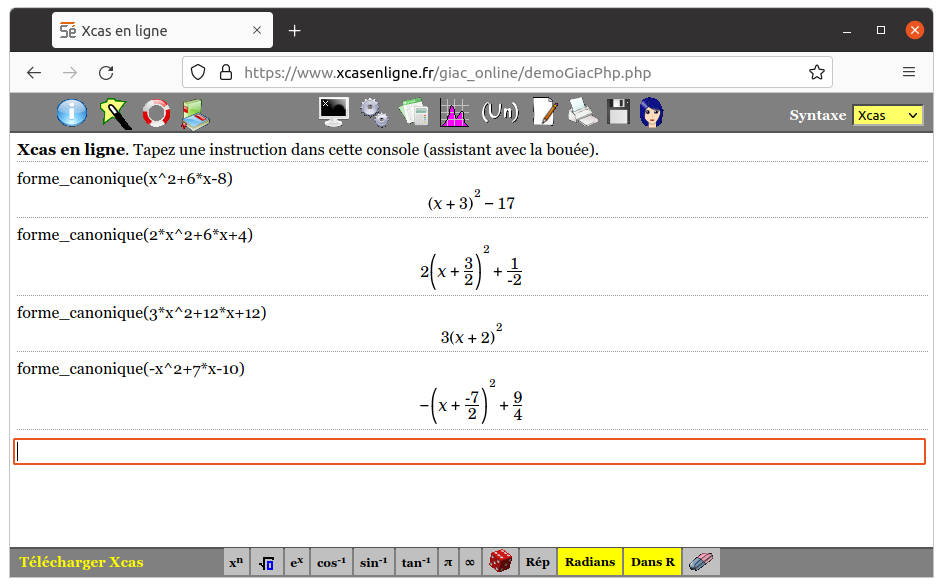
\includegraphics[scale=0.3]{chap01_exos_corr_a}
	\end{center}
%	\begin{center}
%		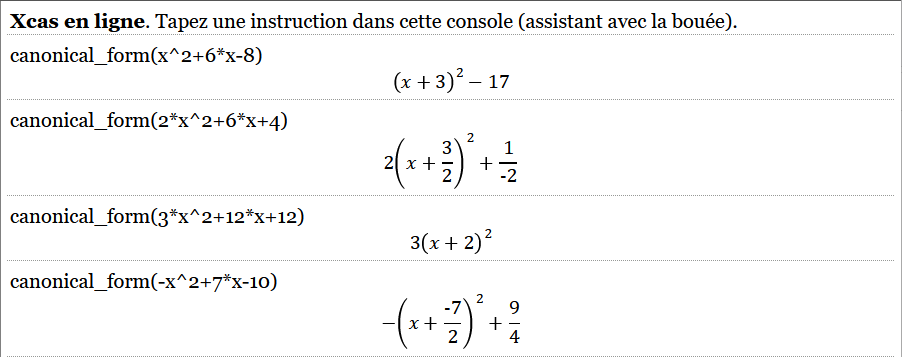
\includegraphics[scale=0.5]{ch01_exos_corr_xcas_1}
%	\end{center}
	\item Pour déterminer le tableau de variation d'un trinôme, on utilise $\alpha$, $\beta$ puis l'\og ouverture \fg{} de la parabole :
	\begin{enumerate}
		\item $f(x)=2(x-4)^2+3$ est sous forme canonique :
		\begin{center}
			\begin{tikzpicture}
				\tkzTabInit{$x$/1,$f$/1.5}{$-\infty$,$4$,$+\infty$}
				\tkzTabVar{+/,-/$3$,+/}
			\end{tikzpicture}
		\end{center}
		\item $g(x)=-3(x+1)^2-5$ est sous forme canonique :
		\begin{center}
			\begin{tikzpicture}
				\tkzTabInit{$x$/1,$g$/1.5}{$-\infty$, $-1$, $+\infty$}
				\tkzTabVar{-/,+/$-5$,-/}
			\end{tikzpicture}
		\end{center}
		\item $h(x)=x(x-8)$ donne la forme canonique $h(x)=(x-4)^2-16$ :
		\begin{center}
			\begin{tikzpicture}
				\tkzTabInit{$x$/1,$h$/1.5}{$-\infty$, $4$, $+\infty$}
				\tkzTabVar{+/,-/$-16$,+/}
			\end{tikzpicture}
		\end{center}
	\end{enumerate}
	\item 
	\begin{enumerate}
		\item On a $f(x)=-2(x-2)^2-5$, et la parabole, \og non souriante \fg{}, a pour sommet $(2\,;\,-5)$.
		\item De ce fait, le maximum de $f$ est $M=-5$, atteint pour $x=2$.
	\end{enumerate}
\end{enumerate}

\medskip

\exonum{0} %exo2

\begin{enumerate}
	\item Pour résoudre les équations, on vérifie que ce sont des équations du 2\up{d} degré \og avec 0 de l'autre côté \fg{}, et si besoin on \og transforme \fg{} :
	\begin{itemize}
		\item on calcule $\Delta=b^2-4ac$ ;
		\item suivant son signe on a :
		\begin{itemize}
			\item aucune racine (et aucune factorisation) si $\Delta < 0$ ;
			\item une racine ($\nicefrac{-b}{2a}$) si $\Delta=0$ ;
			\item deux racines ($\nicefrac{(-b\pm \sqrt{\Delta})}{2a}$) si $\Delta > 0$.
		\end{itemize}
	\end{itemize}
	\begin{center}
		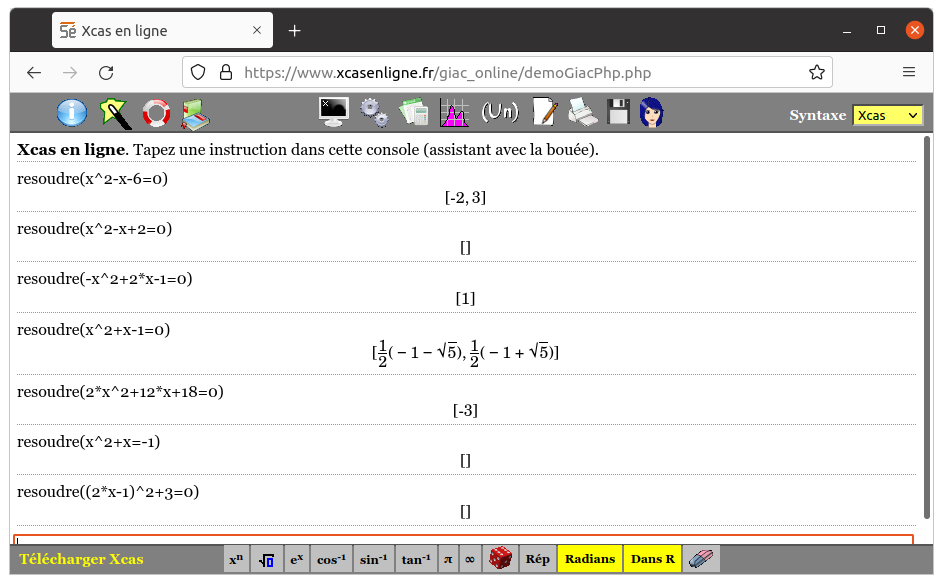
\includegraphics[scale=0.3]{chap01_exos_corr_b}
	\end{center}
	\item Pour écrire un trinôme sous forme factorisée, on calcule ses éventuelles racines (via $\Delta$) puis :
	\begin{itemize}
		\item factorisation $a(x-x_1)(x-x_2)$ si $\Delta>0$ ;
		\item factorisation $a(x-x_0)^2$ si $\Delta=0$ ;
		\item pas de factorisation si $\Delta<0$.
	\end{itemize}
	\begin{center}
		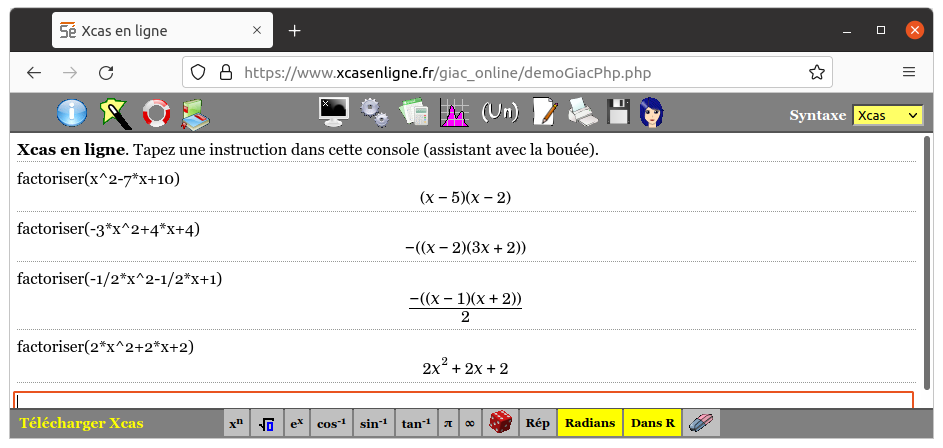
\includegraphics[scale=0.3]{chap01_exos_corr_c}
	\end{center}
%	\begin{center}
%		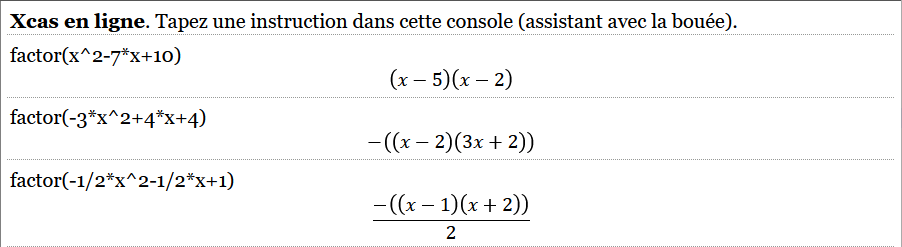
\includegraphics[scale=0.5]{ch01_exos_corr_xcas_5}
%	\end{center}
\end{enumerate}

\medskip

\exonum{0} %exo3

\medskip

On détermine les formes canoniques pour déterminer les tableaux de variations, et donc la courbe correspondante !
\begin{itemize}
	\item \textcolor{blue}{$f_1(x)=-x^2+2x-3=-(x-1)^2-2$ avec le sommet en $(1\,;\,-2)$}.
	\item \textcolor{red}{$f_2(x)=x^2+x+3=(x+0,5)^2+2,75$ avec le sommet en $(-0,5\,;\,2,75)$}.
	\item \textcolor{purple}{$f_3(x)=2x^2-5x+3=-2(x-1,25)^2-0,125$ avec le sommet en $(1,25\,;\,-0,125)$}.
	\item \textcolor{ForestGreen}{$f_4(x)=-2x^2-5x+3=-2(x+1,25)^2+6,125$  avec le sommet en $(-1,25\,;\,6,125)$}.
	\item \textcolor{orange}{$f_5(x)=x^2+x+\dfrac14=(x+0,5)^2$ avec le sommet en $(-0,5\,;\,0)$}.
\end{itemize}

\begin{center}
	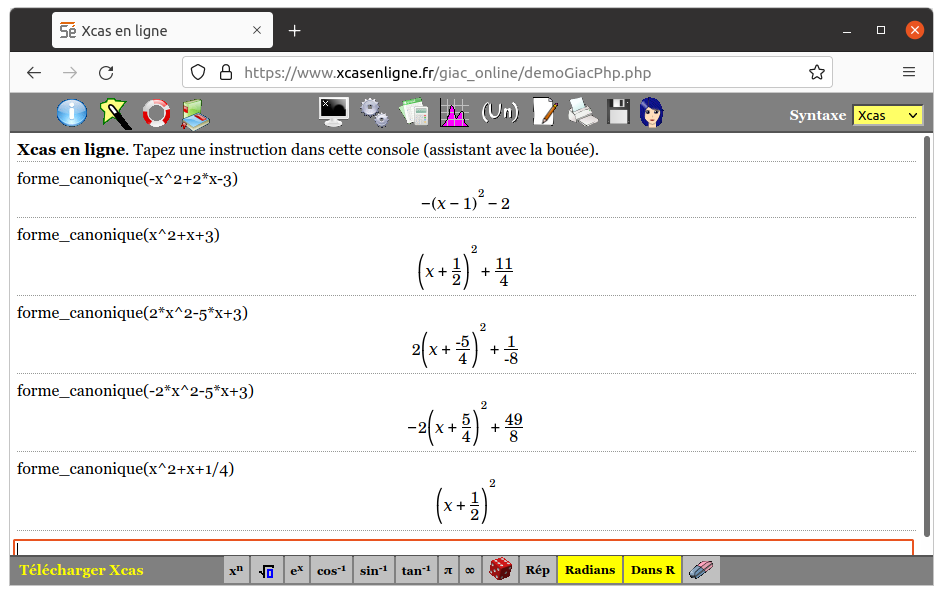
\includegraphics[scale=0.3]{chap01_exos_corr_d}
\end{center}

%\begin{center}
%	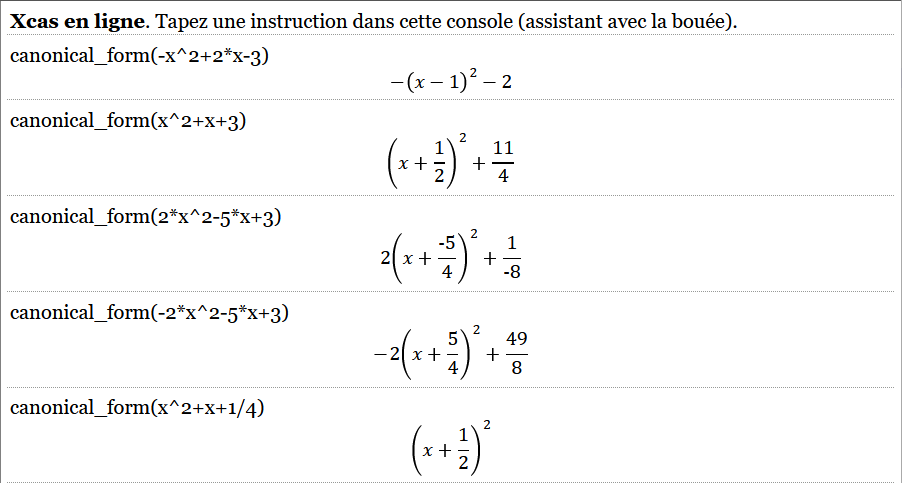
\includegraphics[scale=0.5]{ch01_exos_corr_xcas_6}
%\end{center}

\begin{center}
	\tunits{1}{0.5}
	\tdefgrille{-5}{5}{1}{1}{-6}{7}{1}{1}
	\begin{tikzpicture}[x=\xunit cm,y=\yunit cm]
		%AXES & GRILLES
		\tgrilles[line width=0.4pt,color=lightgray] ;
		\axestikz ;
		\axextikz[size=\small]{-5,-4,...,4} ;
		\axeytikz[size=\small]{-6,-5,...,6} ;
		%LABELS
		\draw (5,2) node[right] {\blue $f_1(x)=-x^2+2x-3$} ;
		\draw (5,1) node[right] {\red $f_2(x)=x^2+x+3$} ;
		\draw (5,0) node[right] {\textcolor{purple}{$f_3(x)=2x^2-5x+3$}} ;
		\draw (5,-1) node[right] {\textcolor{ForestGreen}{$f_4(x)=-2x^2-5x+3$}} ;
		\draw (5,-2) node[right] {\textcolor{orange}{$f_5(x)=x^2+x+\tfrac14$}} ;
		%COURBES
		\clip (\xmin,\ymin) rectangle (\xmax,\ymax) ;
		%		\psplot[linewidth=1.5pt,linecolor=blue]{-5}{5}{-x^2+2*x-3}
		%		\psplot[linewidth=1.5pt,linecolor=red]{-5}{5}{x^2+x+3}
		%		\psplot[linewidth=1.5pt,linecolor=purple]{-5}{5}{2*x^2-5*x+3}
		%		\psplot[linewidth=1.5pt,linecolor=ForestGreen]{-5}{5}{-2*x^2-5*x+3}
		%		\psplot[linewidth=1.5pt,linecolor=orange]{-5}{5}{x^2+x+0.25}
		\draw[line width=1.5pt,blue,domain=-5:5,samples=200] plot(\x,{-\x*\x+2*\x-3});
		\draw[line width=1.5pt,red,domain=-5:5,samples=200] plot(\x,{\x*\x+\x+3});
		\draw[line width=1.5pt,purple,domain=-5:5,samples=200] plot(\x,{2*\x*\x-5*\x+3});
		\draw[line width=1.5pt,ForestGreen,domain=-5:5,samples=200] plot(\x,{-2*\x*\x-5*\x+3});
		\draw[line width=1.5pt,orange,domain=-5:5,samples=200] plot(\x,{\x*\x+\x+0.25});
	\end{tikzpicture}
\end{center}

\medskip

\exonum{2} %exo4

\begin{enumerate}
	\item Pour résoudre les équations suivantes, on les \textbf{transforme} pour se ramener à une équation que l'on sait résoudre :
	\begin{enumerate}
		\item L'équation proposée ne peut pas (encore) être résolue (pb avec le \og $x^3$ \fg), on transforme !
		
		$x^3-8x^2+18x=0 \ssi x(x^2-8x+18)=0$ qui est une \textbf{équation produit} :
		
		\hspace{5mm}$\bullet~~x=0$ ou
		
		\hspace{5mm}$\bullet~~x^2-8x+18=0$ pour lequel $\Delta=-8$ donc pas de solution pour cette \og partie \fg
		
		Ainsi $\mathscr{S}= \left\lbrace \strut 0 \right\rbrace$.
		\item Pour la deuxième équation, on va utiliser le \textbf{produit en croix}, et on a une valeur interdite ($x=-1$).
		
		$\dfrac{x^2+2x+1}{x+1}=2x-1 \ssi x^2+2x+1 = (2x-1)(x+1) \ssi x^2+2x+1 = 2x^2+x-1 \ssi -x^2+x+2 = 0$.
		
		On a $\Delta=9$ et les deux racines sont $x_1=2$ et $x_2=-1$ (valeur interdite !).
		
		Ainsi $\mathscr{S}= \left\lbrace \strut 2 \right\rbrace$.
		\item $\dfrac{3x^2+10x+8}{x+2}=2x+5 \ssi 3x^2+10x+8 = (x+2)(2x+5) \ssi 3x^2+10x+8=2x^2+9x+10$
		
		$\phantom{\dfrac{3x^2+10x+8}{x+2}=2x+5} \ssi x^2+x-2=0$ (avec $x \neq -2$).
		
		On a $\Delta=9$ et les deux racines sont $x_1=1$ et $x_2=-2$ (valeur interdite !).
		
		Ainsi $\mathscr{S}= \left\lbrace \strut 1 \right\rbrace$.
	\end{enumerate}
	\begin{center}
		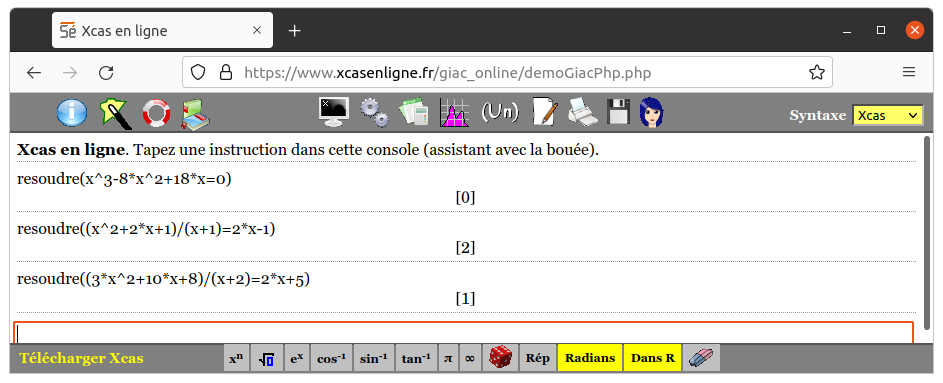
\includegraphics[scale=0.3]{chap01_exos_corr_e}
	\end{center}
%	\begin{center}
%		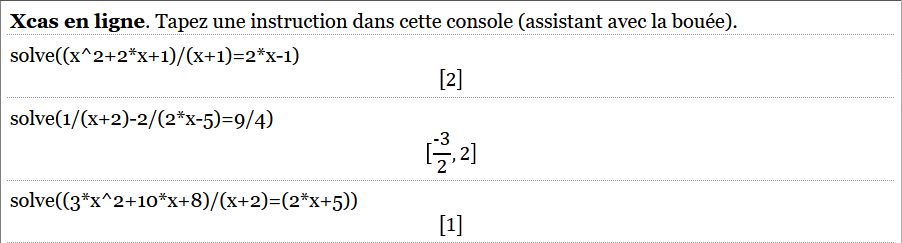
\includegraphics[scale=0.5]{ch01_exos_corr_xcas_3}
%	\end{center}
	\item 
	\begin{enumerate}
		\item L'équation admet une seule racine (double) dans le cas où le discriminant est nul.
		
		Et $\Delta = 0 \ssi b^2-4ac = 0 \ssi (-4)^2 - 4 \times 1 \times (m-1) = 0 \ssi 16-4m+4 = 0 \ssi -4m = -20 \ssi m=5$.
		\item Dans ce cas, la racine (double) vaut $x_0=\dfrac{-b}{2a}=\dfrac{-(-4)}{2 \times 1} = 2$ (c'est l'identité remarquable $x^2-4x+4$ !)
	\end{enumerate}
	\item 
	\begin{enumerate}
		\item 2 est solution de l'équation car $2^2-5 \times 2 + 6 = 4 - 10 + 6 =0$.
		\item La somme des racines vaut $\nicefrac{-b}{a} = 5$ et le produit des racines vaut $\nicefrac{c}{a}=-6$.
		\item On a donc $x_1=2$ et donc $x_1 + x_2 = 5 \Rightarrow x_2 = 5 - 2 =3$.
	\end{enumerate}
	\item 
	\begin{enumerate}
		\item $\begin{dcases} x+y=18 \\xy=65 \end{dcases} \Rightarrow x$ et $y$ sont les racines de $X^2-18X+65$.
		
		On utilise $\Delta$, et on trouve $x=13$ et $y=5$ (ou le contraire\dots)
		\item $\begin{dcases} x+y=4 \\xy=5 \end{dcases} \Rightarrow x$ et $y$ sont les racines de $X^2-4X+5$.
		
		On utilise $\Delta$, et on ne trouve aucune solution\dots
	\end{enumerate}
\end{enumerate}

\medskip

\exonum{2} %exo5

\medskip

On pose $x$ le côté du premier carré, de sorte qu'on cherche $x$ tel que $x^2+(x+1)^2+(x+2)^2=15\,125 $

Et $x^2+(x+1)^2+(x+2)^2=15\,125 \ssi \dots \ssi 3x^2 + 6x-15\,150 = 0$ qui donne $x=70$ (l'autre solution est négative !).

\smallskip

De même, on cherche $x$ tel que $3x^2+6x-15\,122=0$ qui ne donne aucune solution entière !

\medskip

\exonum{2} %exo6

\medskip

On détermine :
\begin{itemize}
	\item l'aire totale du drapeau : $\mathscr{A}_T=4 \times 3=12$ ;
	\item l'aire de la croix : $\mathscr{A}_C = \text{(bde horiz)} + \text{(bde vert)} - \text{(petit carré du milieu en double)} = x \times 4 + x \times 3 - x^2 = -x^2+7x$. 
\end{itemize}
On cherche donc $x$ ($x\pg 0$) tel que $\mathscr{A}_C = 6 \ssi -x^2+7x = 6 \ssi -x^2+7x-6=0$.

On obtient $\Delta = 25$ et la solution (positive) $x=1$ (l'autre vaut $-6$ !)

Donc la bande doit avoir une largeur de 1~m.

\medskip

\exonum{2} %exo7

\begin{pyconcode}
# Calcul de alpha et de beta
from math import *
def analysetrinome(a,b,c):
	alpha = -b/(2*a)
	beta = a*alpha**2 + b*alpha + c
	print(f"Le sommet de la parabole a pour coordonnées ({alpha},{beta})")
	if a > 0 :
		print("La parabole est ouverte vers le haut")
	else :
		print("La parabole est ouverte vers le bas")

\end{pyconcode}

\begin{tcpythoncodeno}[15cm]
	\begin{pyverbatim}[][fontsize=\footnotesize,numbers=none]
		def analysetrinome(a,b,c) :
			alpha = -b/(2*a)
			beta = a*alpha**2 + b*alpha + c
			print(f"Le sommet de la parabole a pour coordonnées ({alpha},{beta})")
			if a > 0 :
				print("La parabole est ouverte vers le haut")
			else :
				print("La parabole est ouverte vers le bas")
	\end{pyverbatim}
\end{tcpythoncodeno}

On peut vérifier sur \cshell{\url{https://python.cpierquet.fr/?from=examples/2m2chap01exos.py}} :

\begin{consolepython}[15cm]
\begin{pyconsole}[][framesep=3mm,frame=single,label={[\scriptsize Début de la console \logopython]\scriptsize Fin de la console \logopython},fontsize=\footnotesize,framerule=1pt,rulecolor=\color{ForestGreen}]
analysetrinome(-1,2,-3)
\end{pyconsole}
\end{consolepython}
\end{document}

\clearpage

% !TeX TXS-program:compile = txs:///pythonlualatex

\documentclass[a4paper,11pt]{article}
\usepackage[pythontex]{cp-base}
\graphicspath{{./graphics/}}
%variables
\donnees[%
	typedoc=CHAPITRE~,
	numdoc=2,
	classe=1\up{ère} 2M2,
	matiere={[SPÉ.MATHS]},
	annee=2021,
	titre=Suites numériques
	]

%formatage
\author{Pierquet}
\title{\nomfichier}
\hypersetup{pdfauthor={Pierquet},pdftitle={\nomfichier},allbordercolors=white,pdfborder=0 0 0,pdfstartview=FitH}
%divers
\lhead{\entete{\matiere}}
\chead{\entete{\lycee}}
%\rhead{\entete{\classe{} - \mois{} \annee}}
\rhead{\entete{\classe{} - Chapitre \thepart}}
\lfoot{\pied{\matiere}}
\cfoot{\logolycee{}}
\rfoot{\pied{\numeropagetot}}

\begin{document}

\pagestyle{fancy}

\part{CH02 - Suites numériques}

\section{Définitions}

\subsection{Vocabulaire et notations}

\begin{cdefi}
Une \textbf{suite numérique} est une liste (infinie) de nombres, appelés \textbf{termes}, qui sont ordonnés et numérotés.

Le premier terme d'une suite $u$ se note $u_1$, le suivant $u_2$, \dots{} et plus généralement, le terme de rang $n$ , appelé aussi \textbf{terme d'indice $n$}, se note $u_n$.

L'ensemble de tous ces termes, qui constitue la suite, est noté $u$ ou plus souvent $(u_n)$.
\end{cdefi}

\begin{crmq}[s]
\begin{itemize}[leftmargin=*,topsep=0pt,parsep=0pt,partopsep=0pt]
	\item Une suite est en fait une fonction définie sur l'ensemble $\N$ des entiers naturels : à chaque entier $n$ elle fait correspondre une et une seule image $u_n$
	\item Comme l'ensemble $\N$ a pour plus petit élément 0, il est très courant de noter $u_0$ le premier terme de la suite. En fonction des situations, on choisira de démarrer à $u_1$ ou $u_0$ (ou même encore d'autres indices) suivant ce qui sera le plus naturel.
\end{itemize}
\end{crmq}

\subsection{Différents modes de définition}

\begin{ccadre}
Il existe plusieurs modes de génération d'une suite :
\begin{itemize}[leftmargin=*]
	\item Avec une formule de \emph{récurrence} : Les termes sont définis \emph{de proche en proche}. Une formule de récurrence explique comment passer d'un terme au suivant. C'est en général une relation entre deux termes consécutifs $u_n$ et $u_{n+1}$. Dans ce cas, il faut également préciser la valeur et l'indice du premier terme de la suite. Pour calculer un terme d'une suite définie par récurrence, il faut \textit{a priori} d'abord calculer tous les termes précédents.
	\item Avec une formule \emph{explicite} : Les termes ne dépendent que de leur rang $n$. On peut calculer n'importe quel terme directement. On se rapproche davantage de la notion de fonction qu'on a l'habitude d'utiliser. $u_n$ est défini à partir d'une formule dépendant de $n$.
\end{itemize}
\end{ccadre}

\begin{cmethode}
Pour bien comprendre et étudier une suite, il est impératif de savoir avant tout si la suite est une suite \textbf{récurrente} ou une suite \textbf{explicite}. Les techniques d'étude ne seront pas les mêmes dans les deux cas.
\end{cmethode}

\begin{cexemple}[s]
\begin{itemize}[leftmargin=*]
	\item La suite $(u_n)$ définie par $\begin{cases}u_0=5& \\u_{n+1}=2u_n-3& \mbox{pour tout } n\in\N 		\end{cases}$ est une suite \textbf{récurrente}.
	
	La formule explique que pour déterminer un terme de la suite, on prend le précédent et on le multiplie par 2 puis on soustrait 3 au résultat, et ainsi de suite en démarrant avec le nombre 5.
	
	$\textcolor{blue}{u_0}=\textcolor{blue}{5}$ d'après l'énoncé.
	
	$\textcolor{red}{u_1}=2\textcolor{blue}{u_0}-3=2\times\textcolor{blue}{5} -3=\textcolor{red}{7} \text{ et } \textcolor{green}{u_2}=2\times \textcolor{red}{7}-3=\textcolor{green}{11} \text{ et } u_3=2\times11-3=19$ etc
	\item La suite $(v_n)$ définie par $v_n=2^n-5 $ pour tout $n \in \N$ est une suite \textbf{explicite}.
	
	La formule explique que, pour calculer le $n$-ième terme de cette suite, on élève 2 à la puissance $n$ puis on soustrait 5. Il n'est pas nécessaire de connaître le terme précédent pour le calculer, seul son \textbf{rang} est nécessaire.
	
	$v_{\textcolor{blue}{0}}=2^{\textcolor{blue}{0}}-5=1-5=-4 \text{ et } v_{\textcolor{red}{1}}=2^{\textcolor{red}{1}}-5=2-5=-3 \text{ et } v_{\textcolor{green}{7}}=2^{\textcolor{green}{7}}-5=128-5=123$ etc
\end{itemize}
\end{cexemple}

\subsection{Méthodes de calculs}

\begin{ccalco}
À la calculatrice, on peut utiliser la touche \ccalg{Ans} pour calculer les termes consécutifs de la suite :
\begin{center}
	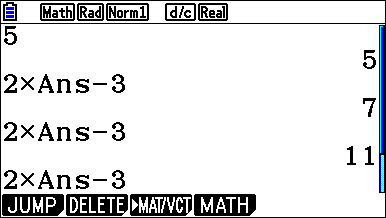
\includegraphics[height=2.25cm]{chap02_suites_ans_90}~~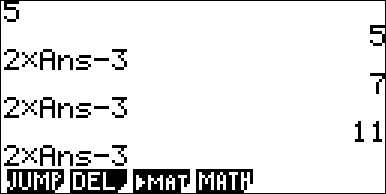
\includegraphics[height=2.25cm]{chap02_suites_ans_35}
\end{center}
\end{ccalco}

\begin{clog}
On peut utiliser un \csheet{tableur} pour calculer les termes d'une suite (explicite ou non), grâce aux références des cellules puis à la \csheet{poignée de recopie} :

\smallskip

\begin{tikzpicture}
	\tableur[4]{A-B}
	\celtxt*[c]{A}{1}{$n$}
	\celtxt*[c]{B}{1}{$u(n)$}
	\celtxt[c]{A}{2}{0}
	\celtxt[c]{A}{3}{1}
	\celtxt[c]{A}{4}{2}
	\selecCell{B}{2}
	\draw[thick,ForestGreen,<-,>=latex'] ($(cellB-2.center)+(4pt,0)$) to [bend right=5] ($(cellB-2)+(2.25,-0.25)$) node[right] {formule explicite en fonction de \textsf{A2}\dots cellule à recopier} ;
\end{tikzpicture}

\smallskip

\begin{tikzpicture}
	\tableur[4]{A-B}
	\celtxt*[c]{A}{1}{$n$}
	\celtxt*[c]{B}{1}{$u(n)$}
	\celtxt[c]{A}{2}{0}
	\celtxt[c]{A}{3}{1}
	\celtxt[c]{A}{4}{2}
	\selecCell{B}{3}
	\draw[thick,ForestGreen,<-,>=latex'] ($(cellB-2.center)+(4pt,0)$) to [bend right=5] ($(cellB-2)+(2.25,-0.25)$) node[right] {terme initial} ;
	\draw[thick,ForestGreen,<-,>=latex'] ($(cellB-3.center)+(4pt,0)$) to [bend right=5] ($(cellB-3)+(2.25,-0.25)$) node[right] {formule de récurrence en fonction de \textsf{B2}, cellule à recopier} ;
\end{tikzpicture}
\end{clog}

\begin{calgo}
On peut utiliser un algorithme, par exemple en \calgpython, pour calculer les termes d'une suite récurrente :
\begin{envpython}[12cm]
	def terme_un(n):
		u = ...                     # 1er terme de la suite
		for i in range(1,...) :     # i va de 1 à ...
			u = .........           # formule de récurrence
		return u
\end{envpython}
\end{calgo}

\section{Représentation graphique}

\subsection{Cas général}

\begin{cmethode}
Pour représenter graphiquement une suite numérique $(u_n)$, on dessine le \textbf{nuage de points} de coordonnées $(n\,;\,u_n)$ pour $n$ entier naturel. On trouve donc en \textbf{abscisses} les \textbf{rangs} $n$ (entiers positifs) et en \textbf{ordonnées} les \textbf{termes} $u_n$.
\end{cmethode}

\begin{cattention}
\textbf{Ces points ne doivent pas être reliés}, contrairement à ce que l'on fait habituellement pour les fonctions. En effet, une fonction est définie sur un intervalle : entre deux valeurs de cet intervalle, on peut toujours en trouver une troisième. Par contre, entre deux nombres entiers consécutifs, il n'y a rien.
\end{cattention}

\begin{crmq}
Cette technique ne diffère pas vraiment de la technique habituelle pour représenter les fonctions : si la suite $(u_n)$ est définie par une formule explicite du type $u_n=f(n)$ , on peut tracer la courbe de la fonction $f$ , puis y matérialiser les points d’abscisse entière !
\end{crmq}

\subsection{Cas d'une suite récurrente}

\begin{cidee}
Dans le cas d'une suite récurrente, on utilise souvent une autre technique, qui a l'avantage de ne pas nécessiter le calcul des termes de la suite, et qui permet de visualiser rapidement certaines propriétés de la suite.
\end{cidee}

\begin{cmethode}
Dans le cas d'une suite récurrente définie par une relation du type $u_{n+1}=f(u_n)$, on peut aussi la représenter sur un axe gradué, en général celui des abscisses :
\begin{itemize}[leftmargin=*]
	\item On cherche l'expression de la fonction $f$ associée.
	\item On la représente dans un repère et on trace également la droite $\Delta$ d'équation $y=x$.
	\item On place le premier terme au niveau de sa valeur sur l'axe des abscisses.
	\item On cherche son image par la fonction $f$ sur l'axe des ordonnées : c'est $u_1$.
	\item On ramène $u_1$ sur l'axe des abscisses grâce à la droite $\Delta$.
	\item Et on recommence\ldots{} on trace alors une \og toile \fg{} en \og escalier \fg{} ou en \og escargot \fg{} qui permet de \textit{conjecturer} beaucoup de choses concernant la suite (sens de variation, existence d'une valeur limite).
\end{itemize}
\end{cmethode}

\begin{cexemple}
Représenter graphiquement la suite récurrente définie par $\begin{cases}u_0=2& \\ u_{n+1}=-0,5u_n+2& \mbox{pour tout } n\in\N \end{cases}$.
\end{cexemple}
	
\begin{cillustr}
\begin{center}
	\tunits{3}{3}
	\tdefgrille{0}{2.5}{0.5}{0.25}{0}{2.5}{0.5}{0.25}
	\begin{tikzpicture}[x=\xunit cm,y=\yunit cm]
		\tikzset{arrowinside/.style 2 args={postaction={decorate},decoration={markings,mark=at position #1 with {\arrow[scale=#2,>=latex]{>}}}}}
		\tikzset{verte/.style={line width=1.5pt,ForestGreen,densely dashed}}
		\tikzset{noire/.style={line width=1.5pt,darkgray,dotted}}
		\tgrilles[line width=0.2pt,color=orange!50] ;
		\tgrillep[line width=0.4pt,color=orange!50] ;
		\axestikz* ;
		\axextikz{0,0.5,1,1.5,2} ;
		\axeytikz{0,0.5,1,1.5,2} ;
		\clip (\xmin,\ymin) rectangle (\xmax,\ymax) ;
		\draw[line width=1.25pt,blue] (0,0) -- (2.5,2.5) ;
		\draw[line width=1.25pt,red,domain=0:2.5] plot (\x,{-0.5*\x+2}) ;
		%lignes vertes
		\draw[verte,arrowinside={0.5}{1.15}] (2,0)--(2,1) ;
		\draw[verte,arrowinside={0.5}{1.15}] (2,1)--(1,1) ;
		\draw[verte,arrowinside={0.5}{1.15}] (1,1)--(1,1.5) ;
		\draw[verte,arrowinside={0.5}{1.15}] (1,1.5)--(1.5,1.5) ;
		\draw[verte,arrowinside={0.5}{1.15}] (1.5,1.5)--(1.5,1.25);
		%lignes noires
		\draw[noire,arrowinside={0.5}{1.15}] (1,1)--(1,0) ;
		\draw[noire,arrowinside={0.5}{1.15}] (1.5,1.5)--(1.5,0) ;
	\end{tikzpicture}
\end{center}
%\begin{center}
%	\psset{unit=3cm,tickwidth=1pt,algebraic=true}
%	\defgrille{0}{2.5}{0.5}{0.25}{0}{2.5}{0.5}{0.25}
%	\begin{pspicture}(0,-0.25)(2.5,2.5)
%		\grilles{linewidth=0.2pt,linecolor=orange!50}
%		\grillep{linewidth=0.4pt,linecolor=orange!50}
%		\psaxes[comma,linewidth=1pt,Dx=0.5,Dy=0.5]{->}(0,0)(2.5,2.5)
%		\psline[linewidth=1.25pt,linecolor=blue](0,0)(2.5,2.5)
%		\psplot[linewidth=1.25pt,linecolor=red]{0}{2.5}{-0.5*x+2}
%		\psset{linewidth=1.5pt,linecolor=ForestGreen,linestyle=dashed,ArrowInside=->,ArrowInsidePos=0.5,arrowscale=1.5}
%		\psline(2,0)(2,1)(1,1)(1,1.5)(1.5,1.5)(1.5,1.25)
%		\psset{linewidth=1.5pt,linecolor=darkgray,linestyle=dotted,ArrowInside=->,ArrowInsidePos=0.5,arrowscale=1.5}
%		\psline(1,1)(1,0)\psline(1.5,1.5)(1.5,0)
%	\end{pspicture}
%\end{center}
\end{cillustr}

\pagebreak

\section{Sens de variation}

\subsection{Définition}

\begin{cdefi}
Une suite $(u_n)$ est dite :
\begin{itemize}
	\item \textbf{Croissante} (à partir de $n_0$) si et seulement si $u_n \pp u_{n+1}$ pour tout $n~ (\pg n_0)$  
	\item \textbf{Décroissante} (à partir de $n_0$) si et seulement si $u_n \pg u_{n+1}$ pour tout $n~ (\pg n_0)$  
	\item \textbf{Constante} (à partir de $n_0$) si et seulement si $u_n = u_{n+1}$ pour tout $n ~(\pg n_0)$ 
	\item \textbf{Monotone} si elle ne change pas de sens de variation
	\item Dans tous les autres cas, on dira simplement que la suite n'est pas monotone.
\end{itemize}
\end{cdefi}

\begin{crmq}
On définit de la même façon une suite strictement croissante ou strictement décroissante, il suffit de changer l'inégalité large par une inégalité stricte !
\end{crmq}

\subsection{Méthodes de recherche}

\begin{cmethode}
Pour étudier le sens de variation d'une suite :
\begin{itemize}
	\item on calcule la différence $u_{n+1}-u_n$ entre deux termes consécutifs ;
	\item on étudie son signe ;
	\item si la différence est toujours \textbf{positive}, alors la suite est \textbf{croissante} et si la différence est toujours \textbf{négative}, alors la suite est \textbf{décroissante}.
\end{itemize}
\end{cmethode}

\begin{crmq}[s]
Dans certains cas, on peut également utiliser d'autres méthodes :
\begin{itemize}
	\item Si la suite est \textbf{explicite} du type $u_n=f(u_n)$, on peut étudier les variations de $f$ sur $\R^{+}$.
	\item Si la suite est une suite de termes \textbf{strictement positifs}, on peut aussi calculer le quotient $\frac{u_{n+1}}{u_n}$ et le comparer à 1.
\end{itemize}
\end{crmq}

\section{Compléments}

\subsection{Limite d'une suite}

\begin{ccadre}
Il ne s'agit cette année que d'avoir une notion intuitive de ce qu'est la limite d'une suite.

\smallskip

S'intéresser à la limite d'une suite $(u_n)$, c'est étudier le comportement des termes lorsque le rang $n$ devient très grand, c'est-à-dire lorsque $n$ tend vers $+ \infty$.

\smallskip

Nous avons vu sur des exemples que, dans certains cas, les termes de la suite semblent être de plus en plus proches d'une certaine valeur $\ell$, on dit alors que la suite \textbf{converge} vers $\ell$, et on écrit  $\lim_{n\to +\infty}u_n=\ell$.

\smallskip

Dans d'autres cas, les termes semblent devenir aussi grands que l'on veut, à condition de choisir $n$ assez grand. On dit que la suite \textbf{diverge} vers + $\infty$ et on écrit $\lim_{n\to +\infty}u_n=+ \infty$.

Une suite peut également diverger vers $- \infty$.

\smallskip

Il arrive aussi que la suite ne semble pas se rapprocher de quoi que ce soit en particulier et n'ait pas de limite. On dit alors aussi qu'elle est \textbf{divergente}.
\end{ccadre}

\subsection{Suites et algorithmes}

\begin{pyconcode}
#terme
def terme_un(n):
	u = 300
	for i in range(1,n+1) :
		u = 1.02 * u
	return u
	

def seuil(S) :
	n = 0					# rang initial
	u = 300					# 300€ disponibles
	while u < S :				# tant qu'on a moins de S euros
		u = 1.02 * u		# on ajoute 2%
		n = n + 1		    # on incrémente
	return n,u
	

def somme_carres(n) :
	u = 1						# le 1er carré vaut 1
	s = 1						# la somme aussi
	for i in range(2,n+1)	:	# i va de 2 à n
		u = i**2		   		# u_1 = i²
		s = s + u		    	# on augment la somme partielle de u
	return s
	

\end{pyconcode}

\begin{ccadre}
Dans le cadre des suites, et tout particulièrement dans celui des suites \textit{récurrentes}, on utilise beaucoup l'algorithmique. Les \calg{boucles} permettent notamment de répéter une instruction (ou une liste d'instructions).

On distingue essentiellement :

\begin{itemize}
	\item la boucle \calg{POUR} ou \calg{FOR}, pour répéter une instruction un \textbf{nombre donné de fois} ;
	\item la boucle \calg{TANT QUE} ou \calg{WHILE}, pour répéter une instruction \textbf{jusqu'à} une condition d'arrêt. (On parle aussi de \textit{boucle conditionnelle})
\end{itemize}

Un passage dans une boucle s'appelle une \calg{itération}.

On utilise une boucle \calg{POUR} quand on connaît à l'avance le nombre d'itérations à effectuer, une boucle \calg{TANTQUE} sinon.
\end{ccadre}

\begin{cpython}
La boucle \calg{POUR} s'écrit dans \calgpython{} :
\vspace{-0.15cm}
\begin{envpython}[15cm]
	# boucle pour
	for <variable> in range(<première itération>,<dernière itération + 1>) :
		<instructions>
\end{envpython}
\faIcon{bomb} Dans \cpy{range} on écrit la première valeur de \cpy{i} utilisée, et la première valeur de \cpy{i} non utilisée.
\end{cpython}

\begin{cpython}
La boucle \calg{TANTQUE} s'écrit dans \calgpython{} :
\vspace{-0.15cm}
\begin{envpython}[15cm]
	#boucle tantque
	while <condition> :
		<instructions>
\end{envpython}
\faIcon{bomb} La \cpy{condition} doit être vérifiée au départ pour qu'on entre dans la boucle.
\end{cpython}

\begin{calgo}[ - Recherche du terme d'une suite récurrente]
Pour calculer un terme donné d'une suite récurrente, on connaît le nombre d'itérations : on utilise donc une boucle \calg{POUR}.

Le programme \calgpython{} ci-dessous permet de calculer les termes de la suite $\suiten$ définie par $\begin{dcases}u_0=300 \\ u_{n+1}= 1,02 \times u_n \end{dcases}$.

\begin{envpython}[15cm]
	def terme_un(n):
		u = 300                     # 1er terme de la suite
		for i in range(1,n+1) :     # i va de 1 à n
			u = 1.02 * u            # formule de récurrence
		return u
\end{envpython}

Pour calculer par exemple $u_7$, il suffira d'appeler dans la \cpy{console} :

\begin{consolepython}[15cm]
\begin{pyconsole}[][framesep=3mm,frame=single,label={[\scriptsize Début de la console \logopython]\scriptsize Fin de la console \logopython},fontsize=\footnotesize,framerule=1pt,rulecolor=\color{ForestGreen}]
terme_un(7)
\end{pyconsole}
\end{consolepython}
\end{calgo}

\begin{calgo}[ - Recherche d'un rang (algorithme de seuil)]
Si on cherche le rang à partir duquel les termes d'une suite vérifient une certaine condition, on ne connait pas le nombre d'itérations à effectuer, donc on utilise une boucle \calg{TANTQUE}.

À chaque itération, on teste la condition : \textit{tant qu'elle est vraie, on continue à calculer} ; \textit{dès qu'elle est fausse, on sort de la boucle}.

Par exemple,une somme de 300\,€ est placée à intérêts composés au taux de 2\,\% par an. On souhaite savoir pendant combien de temps laisser dormir cet argent pour disposer d'au-moins 350\,€.

\begin{envpython}[15cm]
	def seuil(S) :
		n = 0                   # rang initial
		u = 300                 # 300€ disponibles
		while u < S :           # tant qu'on a moins de S euros
			u = 1.02 * u        # on ajoute 2%
			n = n + 1           # on incrémente
		return n,u              # on renvoie le rang et la somme
\end{envpython}

Pour savoir quand on atteindra 350\,€ sur le compte, il suffira d'appeler dans la \cpy{console} :

\begin{consolepython}[15cm]
\begin{pyconsole}[][framesep=3mm,frame=single,label={[\scriptsize Début de la console \logopython]\scriptsize Fin de la console \logopython},fontsize=\footnotesize,framerule=1pt,rulecolor=\color{ForestGreen}]
seuil(350)
\end{pyconsole}
\end{consolepython}

On sait donc qu'il faudra attendre 8 ans et qu'on disposera alors de $u_8 \approx 351,50$\,€. (On remarquera qu'on avait bien trouvé $u_7<350$ avec le programme précédent.)
\end{calgo}

\begin{calgo}[ - Recherche de la somme des termes d'une suite]
Si on veut additionner tous les premiers termes d'une suite avec un programme, il faut calculer la somme \textit{au fur et à mesure} car les termes sont écrasés d'une itération à l'autre.

Par exemple, si on veut calculer la somme de tous les carrés parfaits jusqu'à un rang $n$, autrement dit la somme $1^2+2^2+\dots+n^2$, on peut utiliser :

\begin{envpython}[15cm]
def somme_carres(n) :
	u = 1                       # le 1er carré vaut 1
	s = 1                       # la somme aussi
	for i in range(2,n+1) :     # i va de 2 à n
		u = i**2                # u_i = i²
		s = s + u               # on augmente la somme partielle de u
	return s                    # on affiche la somme complète
\end{envpython}

Dans la console ci-dessous, on voit que la somme des trois premiers carrés est $1^2+ 2^2+ 3^2= 14$, mais aussi que la somme des carrés jusqu'à $100^2$ est égale à \num{338350}, tout aussi rapidement:

\begin{consolepython}[15cm]
\begin{pyconsole}[][framesep=3mm,frame=single,label={[\scriptsize Début de la console \logopython]\scriptsize Fin de la console \logopython},fontsize=\footnotesize,framerule=1pt,rulecolor=\color{ForestGreen}]
somme_carres(3)
somme_carres(100)
\end{pyconsole}
\end{consolepython}
On peut bien sûr calculer aussi la somme des termes d'une suite récurrente en écrivant la formule adéquate pour calculer $u_i$ à la ligne \cpy{5}.
\end{calgo}

\newpage

\subsection{Suites et Représentations graphiques}

\begin{cmanip}[s - Suites explicites]
On considère les suites $\suiten$ et $\suiten[v]$ définies $u_n = \dfrac{1}{n+1}$ et $v_n = 0,25n^2-n$ définies sur $\N$.

À l'aide de la calculatrice, et notamment du module \ccalg{Suites}, représenter graphiquement (nuage de points) les 10 premiers termes des suites $\suiten$ et $\suiten[v]$.
\end{cmanip}

\begin{cillustr}[s - Suites explicites]
\begin{center}
	\tunits{0.6}{4}
	\tdefgrille{0}{10}{1}{1}{0}{1}{0.1}{0.1}
	\begin{tikzpicture}[x=\xunit cm,y=\yunit cm]
			\tgrilles
			\draw[->,line width=1.25pt] (\xmin,0) -- (\xmax,0);
			\draw[->,line width=1.25pt] (0,\ymin) -- (0,\ymax);
			\foreach \x in {0,...,9}
				\draw[line width=1.25pt] (\x,4pt) -- (\x,-4pt) node[below] {\num{\x}};
			\foreach \y in {0,0.2,0.4,0.6,0.8}
				\draw[line width=1.25pt] (4pt,\y) -- (-4pt,\y) node[left] {\num{\y}};
			\draw[thick,red] plot[mark=*,mark size=2pt] coordinates {(3.85,0.925)} node[right] {\large \red $\suiten$};
		\end{tikzpicture}
	~~~~~~~~~~~~
	\tunits{0.6}{0.22}
	\tdefgrille{0}{10}{1}{1}{-4}{16}{2}{2}
	\begin{tikzpicture}[x=\xunit cm,y=\yunit cm]
			\tgrilles
			\draw[->,line width=1.25pt] (\xmin,0) -- (\xmax,0);
			\draw[->,line width=1.25pt] (0,\ymin) -- (0,\ymax);
			\foreach \x in {0,...,9}
				\draw[line width=1.25pt] (\x,4pt) -- (\x,-4pt) node[below] {\num{\x}};
			\foreach \y in {-4,0,...,12}
				\draw[line width=1.25pt] (4pt,\y) -- (-4pt,\y) node[left] {\num{\y}};
			\draw[thick,blue] plot[mark=*,mark size=2pt] coordinates {(3.85,14.5)} node[right] {\large \blue $\suiten[v]$};
		\end{tikzpicture}
\end{center}
\end{cillustr}

\begin{cmanip}[ - Suite récurrente]
On considère la suite récurrente définie par $u_0 = 1$ et $u_{n+1}=1+\dfrac{1}{u_n}$ pour tout entier $n$.

$\bullet~~$Calculer les 10 premières termes de $\suiten$ et représenter graphiquement son nuage de points (graph. v1).

$\bullet~~$En utilisant la technique de la \og toile d'araignée \fg{}, représenter les premiers termes de $\suiten$ (graph. v2).
\end{cmanip}

\begin{cillustr}[ - Suite récurrente (v1)]
\begin{center}
	\tunits{1.5}{1.5}
	\tdefgrille{0}{10}{1}{1}{0}{2.25}{0.25}{0.25}
	\begin{tikzpicture}[x=\xunit cm,y=\yunit cm]
			\tgrilles
			\draw[->,line width=1.25pt] (\xmin,0) -- (\xmax,0);
			\draw[->,line width=1.25pt] (0,\ymin) -- (0,\ymax);
			\foreach \x in {0,...,9}
				\draw[line width=1.25pt] (\x,4pt) -- (\x,-4pt) node[below] {\num{\x}};
			\foreach \y in {0,0.5,1,1.5,2}
				\draw[line width=1.25pt] (4pt,\y) -- (-4pt,\y) node[left] {\num{\y}};
		\end{tikzpicture}
\end{center}
\end{cillustr}

\begin{cillustr}[ - Suite récurrente (v2)]
\begin{center}
	\tunits{5}{1.5}
	\tdefgrille{0}{2.5}{0.5}{0.5}{0}{2.25}{0.25}{0.25}
	\begin{tikzpicture}[x=\xunit cm,y=\yunit cm]
			%axes et grille
			\tgrilles
			\draw[->,line width=1.25pt] (\xmin,0) -- (\xmax,0);
			\draw[->,line width=1.25pt] (0,\ymin) -- (0,\ymax);
			\foreach \x in {0,0.5,...,2}
				\draw[line width=1.25pt] (\x,4pt) -- (\x,-4pt) node[below] {\num{\x}};
			\foreach \y in {0,0.5,...,2}
				\draw[line width=1.25pt] (4pt,\y) -- (-4pt,\y) node[left] {\num{\y}};
			%courbes
			\draw[line width=1.25pt,blue,domain=0:2.25,samples=200,smooth] plot(\x,{\x});
			\draw[line width=1.25pt,red,domain=0.8:2.5,samples=200,smooth] plot(\x,{1+1/\x});
			%labels
			\draw (2.25,2.25) node[below right] {\blue \large $\Delta$};
			\draw (0.8,2.25) node[below left] {\red \large $\mathscr{C}_f$};
		\end{tikzpicture}
\end{center}
\end{cillustr}

\newpage

\subsection{Point histoire}

\begin{chistoire}[ - Source Wikipedia]
Les suites numériques sont liées à la mathématique de la mesure (mesures d'un phénomène prises à intervalles de temps réguliers) et à l'analyse (une suite numérique est l'équivalent discret d'une fonction numérique).

\smallskip

La notion de suite est présente dès qu'apparaissent des \textit{procédés illimités} de calcul. On en trouve, par exemple, chez Archimède, spécialiste des procédés illimités d'approximation (séries géométriques de raison 1/4) pour des calculs d'aires et de volumes, ou en Égypte vers 1700 av. J.-C. et plus récemment au I\up{er} siècle apr. J.-C. dans le procédé d'extraction d'une racine carrée par la méthode de Héron d'Alexandrie.

\smallskip

On retrouve ensuite cette préoccupation plusieurs siècles plus tard (à partir du XV\up{e} siècle) avec la méthode des indivisibles (Cavalieri, Torricelli, Pascal, Roberval).

\smallskip

C'est ainsi que l'on voit Bernoulli, Newton, Moivre, Stirling et Wallis, s'intéresser aux suites pour approcher des valeurs numériques. C'est à Lagrange que l'on doit, semble-t-il, la notation indicielle. L'étude des suites ouvre la porte à celle des séries entières dont le but est d'approcher, non plus des nombres, mais des fonctions. Dans la seconde moitié du XX\up{e} siècle, le développement des calculateurs et des ordinateurs donne un second souffle à l'étude des suites en analyse numérique grâce à la méthode des éléments finis. On en retrouve l'usage aussi dans les mathématiques financières.

\begin{center}
	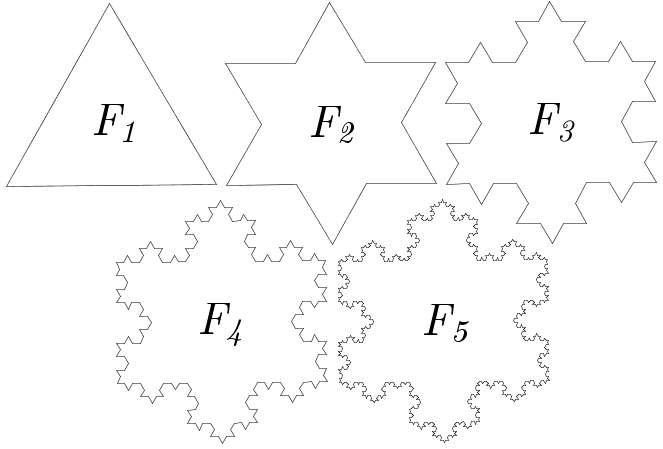
\includegraphics[height=8cm]{chap02_flocons}
\end{center}
\end{chistoire}

\end{document}

\clearpage

\setcounter{numexos}{0}

% !TeX TXS-program:compile = txs:///arara
% arara: lualatex: {shell: no, synctex: yes, interaction: batchmode}
% arara: lualatex: {shell: no, synctex: yes, interaction: batchmode} if found('log', 'undefined references')

\documentclass[a4paper,11pt]{article}
\usepackage[revgoku,breakable]{cp-base}
\graphicspath{{./graphics/}}
%variables
\donnees[%
	classe={1\up{ère} 2M2},matiere={[SPÉ.MATHS]},mois=Octobre,annee=2021,typedoc=CHAP,numdoc=2]
	
%formatage
\author{Pierquet}
\title{\nomfichier}
\hypersetup{pdfauthor={Pierquet},pdftitle={\nomfichier},allbordercolors=white,pdfborder=0 0 0,pdfstartview=FitH}
%divers
\lhead{\entete{\matiere}}
\chead{\entete{\lycee}}
\rhead{\entete{\classe{} - \mois{} \annee}}
\lfoot{\pied{\matiere}}
\cfoot{\logolycee{}}
\rfoot{\pied{\numeropagetot}}

\begin{document}

\pagestyle{fancy}

\part{CH02 - Suites numériques - Exercices}

\smallskip

\begin{caide}
{\setlength\arrayrulewidth{1.5pt} \arrayrulecolor{titrebleu!35}
\begin{tabularx}{\linewidth}{Y|Y|Y|Y|Y|Y}
	\niveaudif{0}~~\textsf{Basique} & \niveaudif{1}~~\textsf{Modérée} & \niveaudif{2}~~\textsf{Élevée} & \niveaudif{3}~~\textsf{Très élevée} & \niveaudif{4}~~\textsf{Extrême} & \niveaudif{5}~~\textsf{Insensée} \\
\end{tabularx}}
\end{caide}

\exonum{0}

\medskip

On considère la suite $\suiten$ définie par $u_n = n^3+3n-1$ pour tout entier $n$.

\begin{enumerate}[itemsep=0pt]
	\item Calculer $u_0$ puis $u_1$.
	\item Calculer la valeur de $u_{10}$.
	\item Exprimer $u_n + 1$ et $u_{n+1}$ en fonction de $n$.
\end{enumerate}

\medskip

\exonum{0}

\medskip

On considère la suite $\suiten$ définie par $u_n=\dfrac{n-3}{n+2}$ pour tout entier $n$.

\begin{enumerate}[itemsep=0pt]
	\item Calculer $u_0$ puis $u_1$.
	\item La suite $\suiten$ est-elle définie par récurrence ou par une formule explicite ?
	\item Déterminer la fonction $f$ associée à la suite $\suiten$.
	\item Calculer la valeur de $u_{50}$.
\end{enumerate}

\medskip

\exonum{1}

\medskip

On considère la suite $\suiten$ définie par $u_0=4$ et $u_{n+1}=2u_n-3$ pour tout entier $n$.

\begin{enumerate}[itemsep=0pt]
	\item Calculer $u_1$ et $u_2$.
	\item La suite $\suiten$ est-elle définie par récurrence ou par une formule explicite ?
	\item Déterminer la fonction $f$ associée à la suite $\suiten$.
	\item Déterminer, en utilisant le module \ccalg{Suites} de la calculatrice, la valeur de $u_{15}$.
\end{enumerate}

\medskip

\exonum{1}

\medskip

On considère la suite $\suiten$ définie par $u_0=1$ et $u_{n+1}=\dfrac{u_n+2}{u_n^2+1}$ pour tout entier $n$.

\begin{enumerate}[itemsep=0pt]
	\item Calculer les valeurs de $u_1$ et $u_2$.
	\item La suite $\suiten$ est-elle définie par récurrence ou par une formule explicite ?
	\item Déterminer la fonction $f$ associée à la suite $\suiten$.
	\item Déterminer, en utilisant le module \ccalg{Suites} de la calculatrice, la valeur de $u_{20}$.
\end{enumerate}

\medskip

\exonum{1}

\medskip

On considère la suite $\suiten$ définie par $u_0=10$ et $u_{n+1}=n-u_n$ pour tout entier $n$.

\begin{enumerate}[itemsep=0pt]
	\item Calculer les valeurs de $u_1$ et $u_2$.
	\item Déterminer, en utilisant le module \ccalg{Suites} de la calculatrice, la valeur de $u_{18}$.
\end{enumerate}

\medskip

\exonum{3}

\medskip

On considère la suite $\suiten[v]$ définie par $v_1=4$ et $v_{n+1}=\dfrac{(n+1)v_n}{n(1+v_n)}$ pour tout entier $n$.

\begin{enumerate}[itemsep=0pt]
	\item Calculer les valeurs de $v_2$, $v_3$ et $v_4$.
	\item Déterminer, en utilisant le module \ccalg{Suites} de la calculatrice, la valeur de $v_{11}$.
\end{enumerate}

\newpage

\exonum{2}

\medskip

On considère la suite $\suiten$ définie par $u_n=\dfrac{(-1)^n}{n+1}$ pour tout entier $n$.

\begin{enumerate}[itemsep=0pt]
	\item Calculer les valeurs de $v_0$, $v_1$, $v_2$, $v_3$ et $v_4$.
	\item Démontrer que $v_{2n}>0$ pour tout entier $n$, et que $v_{2n+1}<0$ pour tout entier $n$.
\end{enumerate}

\medskip

\exonum{1}

\medskip

On considère la suite $\suiten[w]$ définie par $w_n = \dfrac{2}{5^n}$ pour tout entier $n$.

\begin{enumerate}[itemsep=0pt]
	\item Calculer $w_0$, $w_1$, $w_2$ et $w_3$.
	\item Montrer que le quotient $\dfrac{w_{n+1}}{w_n}$ est indépendant de $n$ pour tout entier $n$.
\end{enumerate}

\medskip

\exonum{3}

\medskip

On considère la suite $\suiten$ définie par $u_n = 1 + \frac{1}{n}$ pour tout entier naturel $n$ non nul.

\begin{enumerate}[itemsep=0pt]
	\item Calculer les 3 premiers termes de la suite $\suiten$ ainsi que le 15\up{ème}.
	\item Représenter, dans le repère suivant (l'unité verticale est à préciser), les 10 premiers termes de $\suiten$.
	\begin{center}
		\tunits{1}{1}
		\tdefgrille{0}{10}{1}{1}{0}{2.5}{0.5}{0.5}
		\begin{tikzpicture}[x=\xunit cm,y=\yunit cm]
			\tgrilles[line width=0.4pt,lightgray] ;
			\axestikz* ;
			\axextikz{0,1,...,9} ;
			\foreach \y in {0,0.5,1,1.5,2}
				\draw[line width=1.25pt] (4pt,\y) -- (-4pt,\y) ;
		\end{tikzpicture}
	\end{center}
%	\begin{center}
%		\psset{xunit=1cm,yunit=1cm,tickwidth=1pt,algebraic=true,arrowscale=1.5}
%		\defgrille{0}{10}{1}{1}{0}{2.5}{0.5}{0.5}
%		\begin{pspicture}(0,-0.25)(10,2.5)
%			\grilles{linewidth=0.4pt,linecolor=lightgray}
%			\psaxes[labels=x,linewidth=1pt,Dy=0.5]{->}(0,0)(10,2.5)
%			%\psplot{1}{10}{1+1/x}
%		\end{pspicture}
%	\end{center}
	\item Conjecturer le sens de variation ainsi que la limite éventuelle de la suite $\suiten$.
	\item 
	\begin{enumerate}
		\item Montrer que $u_{n+1}-u_n = \frac{-1}{n(n+1)}$ pour tout entier $n$ non nul.
		\item En déduire le sens de variation de la suite $\suiten$.
	\end{enumerate}
	\item Montrer que $u_n >1$ pour tout entier $n$ non nul (on dit que $\suiten$ est \textbf{minorée} par 1).
\end{enumerate}

\medskip

\exonum{3}

\medskip

On considère la suite $\suiten[v]$ définie par $v_0=2$ et $v_{n+1}=-0,25v_n^2+v_n$ pour tout entier $n$.

\begin{enumerate}[itemsep=0pt]
	\item Calculer $v_1$, $v_2$ et $v_3$.
	\item 
	\begin{enumerate}
		\item Déterminer la fonction $f$ telle que $v_{n+1} = f(v_n)$.
		\item À l'aide de la courbe $\mathscr{C}_f$ donnée ci-dessous, représenter graphiquement les premiers termes de $\suiten[v]$.
		\begin{center}
			\tunits{4}{3}
			\tdefgrille{0}{2.5}{0.25}{0.25}{0}{1.25}{0.25}{0.25}
			\begin{tikzpicture}[x=\xunit cm,y=\yunit cm]
				\tgrilles[line width=0.4pt,lightgray] ;
				\axestikz* ;
				\axextikz{0,1,2} ;
				\foreach \y in {0,0.5,1.0}
					\draw[line width=1.25pt] (4pt,\y) -- (-4pt,\y) node[left] {\num{\y}} ;
				\clip (\xmin,\ymin) rectangle (\xmax,\ymax) ;
				\draw[line width=1.25pt,red](0,0) -- (1.25,1.25) ;
				\draw[line width=1.25pt,blue,domain=0:2.5,samples=200] plot (\x,{-0.25*\x*\x+\x}) ;
				\draw (1.25,1.25) node[below right] {\large \red $\Delta$ : $y=x$} ;
				\draw (2,1) node[above right] {\large \blue $\mathscr{C}_f$} ;
			\end{tikzpicture}
		\end{center}
%		\begin{center}
%			\psset{xunit=4cm,yunit=3cm,tickwidth=1pt,algebraic=true,arrowscale=1.5}
%			\defgrille{0}{2.5}{0.25}{0.25}{0}{1.25}{0.25}{0.25}
%			\begin{pspicture}(-0.25,-0.25)(2.5,1.25)
%				\grilles{linewidth=0.4pt,linecolor=lightgray}
%				\psaxes[comma,linewidth=1pt,Dy=0.5]{->}(0,0)(2.5,1.25)
%				\psline[linewidth=1.25pt,linecolor=red](0,0)(1.25,1.25)
%				\psplot[linewidth=1.25pt,linecolor=blue]{0}{2.5}{-0.25*x^2+x}
%				\uput[dr](1.25,1.25){\large \red $\Delta$ : $y=x$}
%				\uput[ur](2,1){\large \blue $\mathscr{C}_f$}
%			\end{pspicture}
%		\end{center}
		\item Conjecturer le sens de variation ainsi que la limite éventuelle de la suite $\suiten[v]$.
	\end{enumerate}
	\item Calculer $v_{n+1}-v_n$ pour tout entier naturel $n$ puis en déduire le sens de variation de la suite $\suiten[v]$.
\end{enumerate}



\end{document}

\clearpage

\setcounter{numexos}{0}

% !TeX document-id = {52afcdfc-e5de-44c9-a0fc-d554c25c3963}
% !TeX TXS-program:compile = txs:///arara
% arara: lualatex: {shell: no, synctex: yes, interaction: batchmode}
% arara: lualatex: {shell: no, synctex: yes, interaction: batchmode} if found('log', 'undefined references')

\documentclass[a4paper,11pt]{article}
\usepackage[revgoku,breakable]{cp-base}
\graphicspath{{./graphics/}}
%variables
\donnees[%
	classe={1\up{ère} 2M2},matiere={[SPÉ.MATHS]},mois=Octobre,annee=2021,typedoc=CHAP,numdoc=2]

%formatage
\author{Pierquet}
\title{\nomfichier}
\hypersetup{pdfauthor={Pierquet},pdftitle={\nomfichier},allbordercolors=white,pdfborder=0 0 0,pdfstartview=FitH}
%divers
\lhead{\entete{\matiere}}
\chead{\entete{\lycee}}
\rhead{\entete{\classe{} - \mois{} \annee}}
\lfoot{\pied{\matiere}}
\cfoot{\logolycee{}}
\rfoot{\pied{\numeropagetot}}

\begin{document}

\pagestyle{fancy}

\part{CH02 - Suites numériques - Exercices (Correction)}

\smallskip

\exonum{0}

\begin{enumerate}[itemsep=0pt]
	\item On a (formule explicite) $u_0=0^3+3 \times 0 -1 = -1$ et $u_1=1^3+3\times1-1=3$.
	\item On a, de même, $u_{10}=10^3+3\times10-1=\num{1029}$.
	\item \begin{itemize}[leftmargin=*]
		\item On a ${\red u_n} + 1 = {\red n^3+3n-1}+1=n^3+3n$ ;
		\item $u_{\red n+1}=({\red n+1})^3+3({\red n+1})-1=n^3+3n^2+3n+1+3n+3-1=n^3+3n^2+6n$. (qui est différent de $u_n + 1$ !)
	\end{itemize}
\end{enumerate}

\medskip

\exonum{0}

\begin{enumerate}[itemsep=0pt]
	\item On a (formule explicite) $u_0=\dfrac{0-3}{0+2}=-1,5$ et $u_1=\dfrac{1-3}{1+2}=-\dfrac{2}{3}$.
	\item La suite $\suiten$ est définie par une formule explicite.
	\item La fonction $f$ associée à la suite $\suiten$ est $f(x)=\dfrac{x-3}{x+2}$ (on remplace $n$ par $x$ !).
	\item On a $u_{50}=\dfrac{50-3}{50+2}=\dfrac{47}{52}$.
\end{enumerate}

\medskip

\exonum{1}

\begin{enumerate}[itemsep=0pt]
	\item On a (formule de récurrence) :
	\begin{itemize}
		\item $u_1=2u_0-3=2 \times 4 -3 = 5$ ;
		\item $u_2=2u_1-3=2 \times 5 - 3=7$.
	\end{itemize}
	\item La suite $\suiten$ est définie par récurrence.
	\item La fonction $f$ associée à la suite $\suiten$ est $f(x)=2x-3$ (on remplace $u_n$ par $x$ !).
	\item Le module \ccalg{Suites} de la calculatrice donne $u_{15}=\num{32771}$.
	\begin{center}
		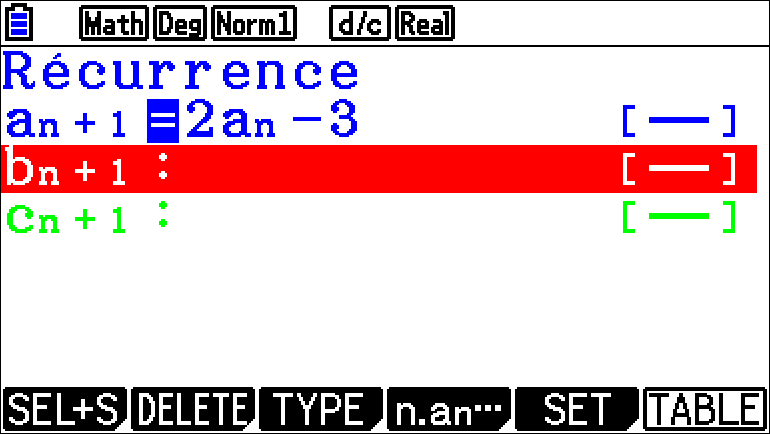
\includegraphics[height=2.5cm]{chap02_exos_corr_3a}~~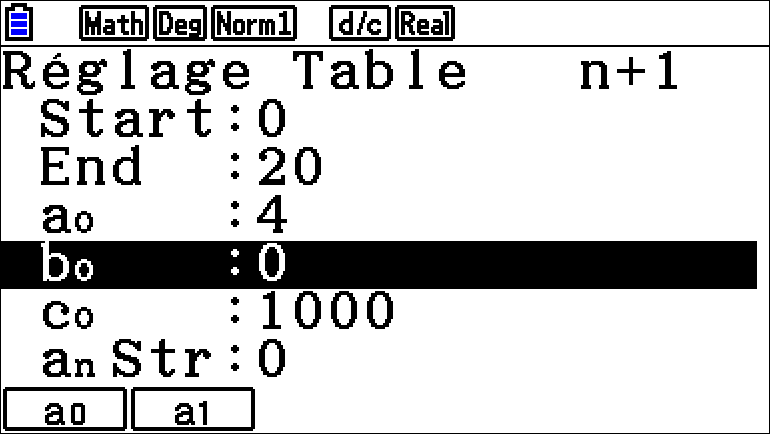
\includegraphics[height=2.5cm]{chap02_exos_corr_3b}~~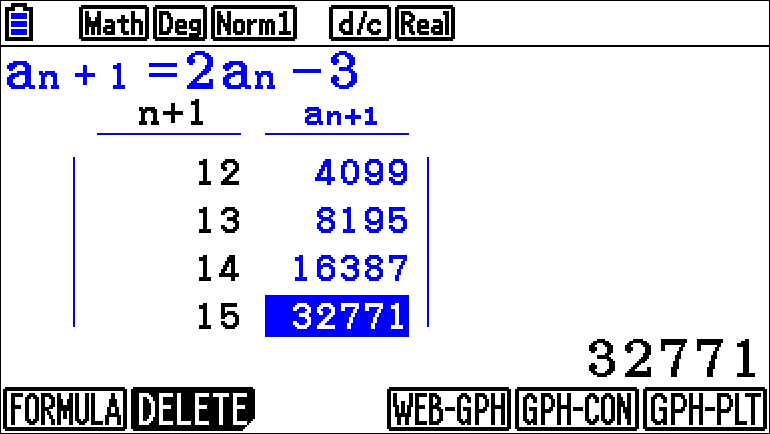
\includegraphics[height=2.5cm]{chap02_exos_corr_3c}
	\end{center}
\end{enumerate}

\medskip

\exonum{1}

\begin{enumerate}[itemsep=0pt]
	\item On a (formule de récurrence) :
	\begin{itemize}
		\item $u_1=\dfrac{u_0+2}{u_0^2+1}=\dfrac{1+2}{1^2+1}=\dfrac{3}{2}=1,5$ ;
		\item $u_2=\dfrac{u_1+2}{u_1^2+1}=\dfrac{1,5+2}{1,5^2+1}=\dfrac{14}{13}$.
	\end{itemize}
	\item La suite $\suiten$ est définie par récurrence.
	\item La fonction $f$ associée à la suite $\suiten$ est $f(x)=\dfrac{x+2}{x^2+1}$ (on remplace $u_n$ par $x$ !).
	\item Le module \ccalg{Suites} de la calculatrice donne $u_{20}\approx 1,2517$ (arrondi à $10^{-4}$).
	\begin{center}
		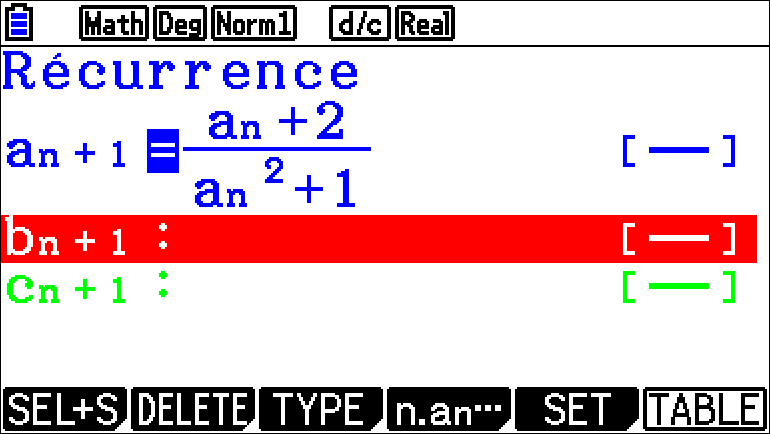
\includegraphics[height=2.5cm]{chap02_exos_corr_4a}~~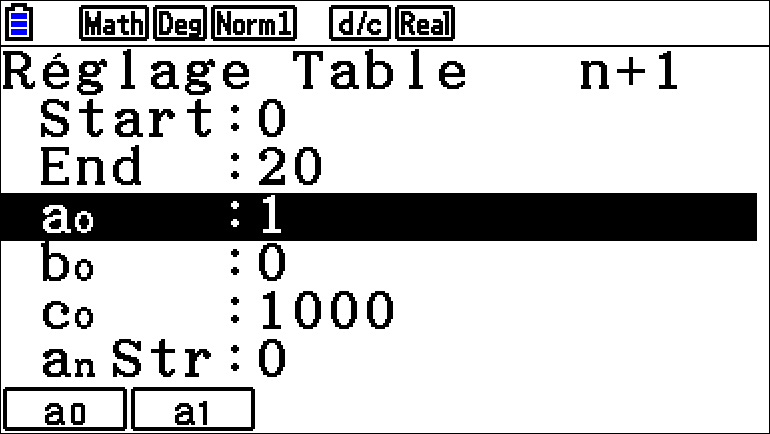
\includegraphics[height=2.5cm]{chap02_exos_corr_4b}~~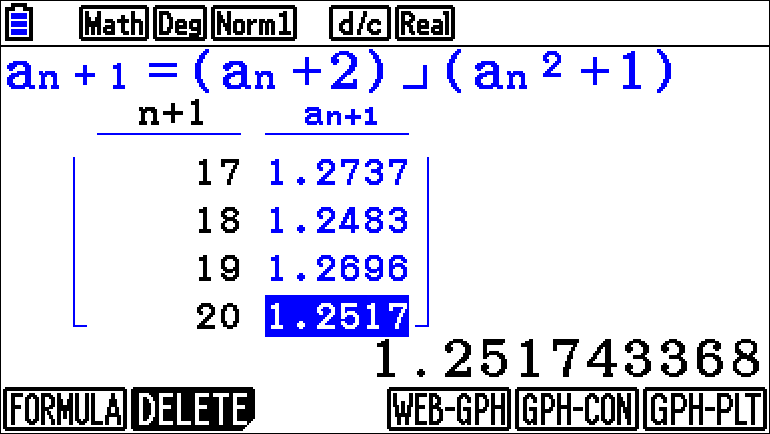
\includegraphics[height=2.5cm]{chap02_exos_corr_4c}
	\end{center}
\end{enumerate}

\medskip

\exonum{1}

\begin{enumerate}[itemsep=0pt]
	\item Il s'agit d'une suite récurrente \og non classique \fg{} pour laquelle il faut respecter la concordance d'indice !
	
	$u_{{\red n}+1}={\red n}-u_{{\red n}}$ :
	\begin{itemize}
		\item $u_1=u_{{\red 0}+1}={\red 0}-u_{\red 0}=0-10=-10$ ;
		\item $u_2=u_{{\red 1}+1}={\red 1}-u_{\red 1}=1-(-10)=11$.
	\end{itemize}
	\item Le module \ccalg{Suites} de la calculatrice donne $u_{18}=19$.
	\begin{center}
		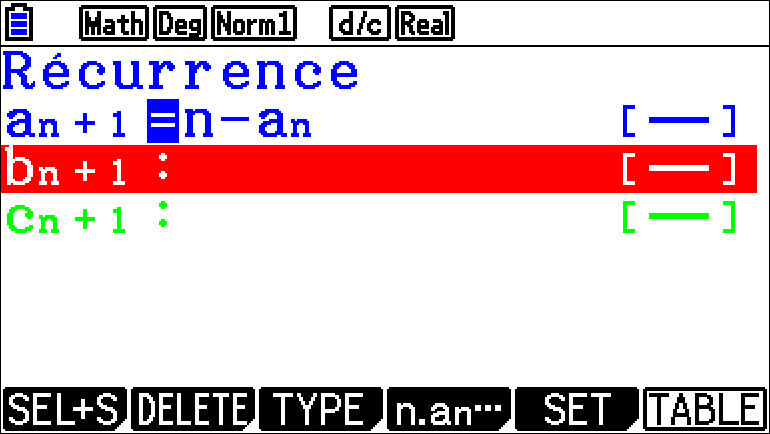
\includegraphics[height=2.5cm]{chap02_exos_corr_5a}~~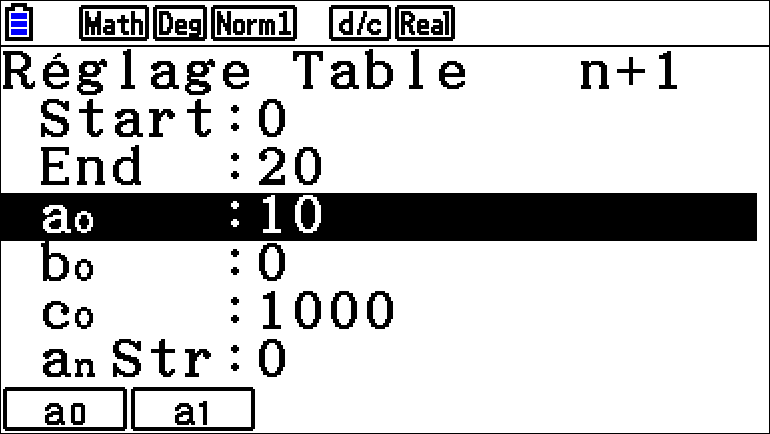
\includegraphics[height=2.5cm]{chap02_exos_corr_5b}~~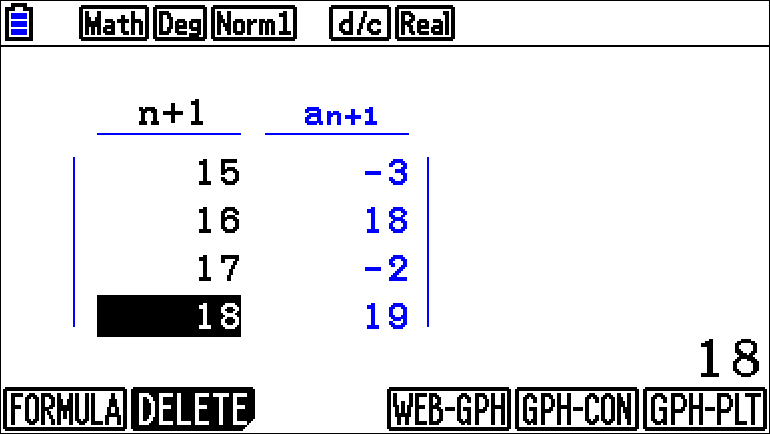
\includegraphics[height=2.5cm]{chap02_exos_corr_5c}
	\end{center}
\end{enumerate}

\medskip

\exonum{3}

\begin{enumerate}[itemsep=0pt]
	\item Il s'agit d'une suite récurrente \og non classique \fg{} pour laquelle il faut respecter la concordance d'indice !
	
	$v_{{\red n}+1}=\dfrac{({\red n}+1)v_{\red n}}{{\red n}(1+v_{\red n})}$ :
	\begin{itemize}
		\item $v_2=v_{{\red 1}+1}=\dfrac{({\red 1}+1)v_{\red 1}}{{\red 1}(1+v_{\red 1})}=\dfrac{2v_1}{1(1+v_1)}=\dfrac{2 \times 4}{1+4}=1,6$ ;
		\item $v_3=v_{{\red 2}+1}=\dfrac{({\red 2}+1)v_{\red 2}}{{\red 2}(1+v_{\red 2})}=\dfrac{3v_2}{2(1+v_2)}=\dfrac{12}{13}$ ;
		\item $v_4=v_{{\red 3}+1}=\dfrac{({\red 3}+1)v_{\red 3}}{{\red 3}(1+v_{\red 3})}=\dfrac{4v_3}{3(1+v_3)}=0,64$.
	\end{itemize}
	\item Le module \ccalg{Suites} de la calculatrice donne $v_{11}=\dfrac{44}{221}\approx 0,199$ (arrondi au millième).
	\begin{center}
		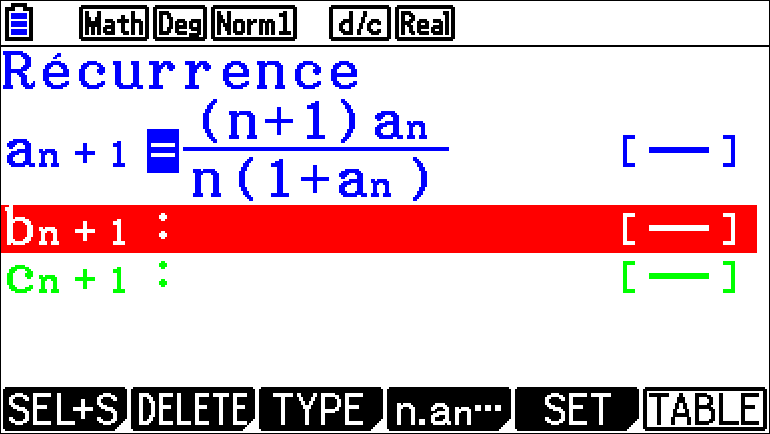
\includegraphics[height=2.5cm]{chap02_exos_corr_6a}~~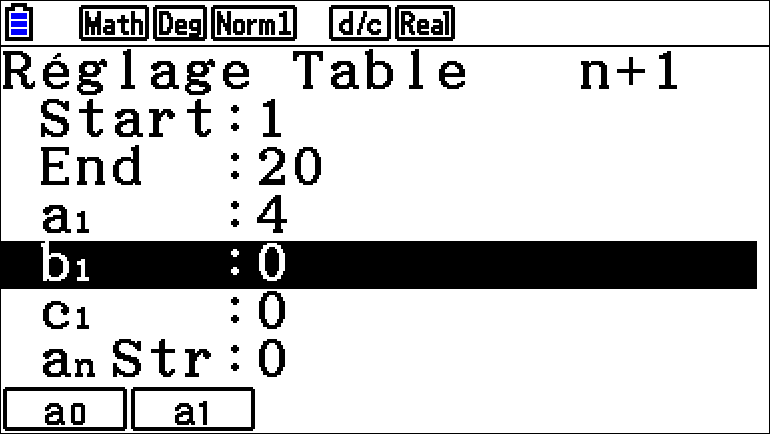
\includegraphics[height=2.5cm]{chap02_exos_corr_6b}~~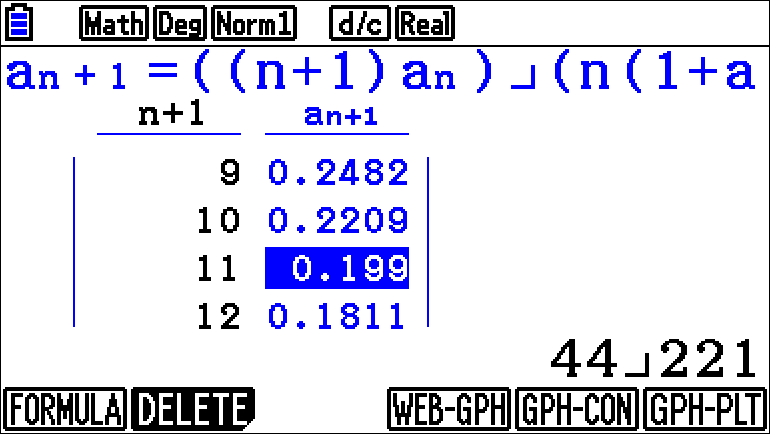
\includegraphics[height=2.5cm]{chap02_exos_corr_6c}
	\end{center}
\end{enumerate}

\medskip

\exonum{2}

\begin{enumerate}[itemsep=0pt]
	\item On a $v_0=\dfrac{(-1)^0}{0+1}=1$ et $v_1=\dfrac{(-1)^1}{1+1}=-0,5$ et $v_2=\dfrac{(-1)^2}{2+1}=\dfrac13$ et $v_3=\dfrac{(-1)^1}{3+1}=-0,25$ et $v_4=\dfrac{(-1)^4}{4+1}=0,2$.
	\item On a :
	\begin{itemize}
		\item $v_{2n}=\dfrac{(-1)^{2n}}{(2n)+1}=\dfrac{1}{2n+1} > 0$ ;
		\item $v_{2n+1}=\dfrac{(-1)^{2n+1}}{(2n+1)+1}=\dfrac{-1}{2n+2} < 0$.
	\end{itemize}
\end{enumerate}

\pagebreak

\exonum{1}

\begin{enumerate}[itemsep=0pt]
	\item On a (formule explicite) $w_0=\dfrac{2}{5^0}=2$ et  $w_1=\dfrac{2}{5^1}=0,4$ et $w_2=\dfrac{2}{5^2}=0,08$ et $w_3=\dfrac{2}{5^3}=0,016$.
	\item On a $\dfrac{w_{n+1}}{w_n} = \dfrac{\tfrac{2}{5^{n+1}}}{\tfrac{2}{5^{n}}}=\dfrac{2}{5^{n+1}} \times \dfrac{5^n}{2}=\dfrac{5^n}{5^{n+1}}=\dfrac{5^n}{5^n \times 5}=\dfrac{1}{5}$ qui est bien indépendant de $n$ !
\end{enumerate}

\medskip

\exonum{3}

\begin{enumerate}[itemsep=0pt]
	\item On a (formule explicite) $u_1=1+\dfrac11=2$ et $u_2=1+\dfrac12=1,5$ et $u_3=1+\dfrac13=\dfrac43$ puis $u_{15}=1+\dfrac{1}{15}=\dfrac{16}{15}$.
	\item On représente le nuage de points :
	\begin{center}
		\tunits{1}{1}
		\tdefgrille{0}{10}{1}{1}{0}{2.5}{0.5}{0.5}
		\begin{tikzpicture}[x=\xunit cm,y=\yunit cm]
			\tgrilles[line width=0.4pt,lightgray]
			\axestikz* \axextikz{0,1,...,9} \axeytikz{0,0.5,1,1.5,2}
			\foreach \n in {1,2,...,10}
				\filldraw[red] (\n,{1+1/\n}) circle[radius=2.5pt] ;
		\end{tikzpicture}
	\end{center}
	\item On peut conjecturer que $\suiten$ est monotone décroissante et convergente vers $\ell=1$.
	\item 
	\begin{enumerate}[itemsep=0pt]
		\item On a $u_{n+1}-u_n = 1+\dfrac{1}{n+1} - \left( 1+\dfrac{1}{n} \right) = \dfrac{1}{n+1} - \dfrac{1}{n} = \dfrac{n}{n(n+1)} - \dfrac{n+1}{n(n+1)} = \dfrac{n-(n+1)}{n(n+1)} = \dfrac{-1}{n(n+1)}$.
		\item par quotient, on a $u_{n+1}-u_n < 0$ (pour tout $n$ non nul), ce qui justifie que $\suiten$ est monotone décroissante.
	\end{enumerate}
	\item Sachant que $\dfrac{1}{n} >0$, on en déduit que $u_n >1$ pour tout entier $n$ non nul.
\end{enumerate}

\medskip

\exonum{3}

\begin{enumerate}[itemsep=0pt]
	\item On a (formule de récurrence) :
	\begin{itemize}
		\item $v_1=-0,25v_0^2+v_0=-0,25 \times 2^2+2 = 1$ ;
		\item $v_2=-0,25v_1^2+v_1=-0,25 \times 1^2+1 = 0,75$ ;
		\item $v_3=-0,25v_2^2+v_2=-0,25 \times 0,75^2+0,75 = \dfrac{39}{64} = \num{0,609375}$.
	\end{itemize}
	\item 
	\begin{enumerate}[itemsep=0pt]
		\item La fonction $f$ telle que $v_{n+1} = f(v_n)$ est $f(x)=-0,25x^2+x$ (on remplace $u_n$ par $x$ !).
		\item À l'aide de la technique de la \og toile \fg{} :
		\begin{center}
			\tunits{4}{3}
			\tdefgrille{0}{2.5}{0.25}{0.25}{0}{1.25}{0.25}{0.25}
			\begin{tikzpicture}[x=\xunit cm,y=\yunit cm]
				\tgrilles[line width=0.4pt,lightgray] ;
				\axestikz \axextikz{0,1,2} ;
				\foreach \y in {0,0.25,0.5,0.75,1.0}
					\draw[line width=1.25pt] (4pt,\y) -- (-4pt,\y) node[left] {\num{\y}} ;
				\clip (\xmin,\ymin) rectangle (\xmax,\ymax) ;
				\draw[line width=1.25pt,red](0,0) -- (1.25,1.25) ;
				\draw[line width=1.25pt,blue,domain=0:2.5,samples=200] plot (\x,{-0.25*\x*\x+\x}) ;
				\draw (1.25,1.25) node[below right] {\large \red $\Delta$ : $y=x$} ;
				\draw (2,1) node[above right] {\large \blue $\mathscr{C}_f$} ;
				\draw[ForestGreen,ultra thick] (2,0)--(2,1)--(1,1)--(1,0.75)--(0.75,0.75)--(0.75,0.609375)--(0.609375,0.609375)--(0.609375,0.51654)--(0.51654,0.51654) ;
			\end{tikzpicture}
		\end{center}
		\item On peut conjecturer que $\suiten[v]$ est monotone décroissante et convergente vers $\ell=0$.
	\end{enumerate}
	\item On a $v_{n+1}-v_n=-0,25v_n^2+v_n-v_n=-0,25v_n^2 < 0$ pour tout entier naturel $n$, donc on en déduit que $\suiten[v]$ est décroissante.
\end{enumerate}

\end{document}

\clearpage

% !TeX TXS-program:compile = txs:///pythonlualatex

\documentclass[a4paper,11pt]{article}
\usepackage[pythontex]{cp-base} %avec options possibles parmi breakable (tcbox), sujetl (exos),  (pour faire "comme avant"), etc...
\graphicspath{{./graphics/}}
%variables
\donnees[%
	typedoc=CHAPITRE~,
	numdoc=3,
	classe=1\up{ère} 2M2,
	matiere={[SPÉ.MATHS]},
	annee=2021,
	titre=Droites et fonctions affines
]

%formatage
\author{Pierquet}
\title{\nomfichier}
\hypersetup{pdfauthor={Pierquet},pdftitle={\nomfichier},allbordercolors=white,pdfborder=0 0 0,pdfstartview=FitH}
%divers
\lhead{\entete{\matiere}}
\chead{\entete{\lycee}}
\rhead{\entete{\classe{} - Chapitre \thepart}}
\lfoot{\pied{\matiere}}
\cfoot{\logolycee{}}
\rfoot{\pied{\numeropagetot}}

\begin{document}

\pagestyle{fancy}

\part{CH03 - Droites et fonctions affines}

\section{Généralités}

\subsection{Définition}

\begin{cdefi}
Une fonction $f$ est \textbf{affine} s'il existe deux réels $m$ et $p$ tels que $f(x)=mx+p$.

Son programme de calcul ne comporte qu'une multiplication (ou division) et une addition (ou soustraction).
\end{cdefi}

\begin{crmq}[s]
$\bullet~~$On utilise aussi souvent les notations $f(x)=ax+b$, qui sont parfois plus ambigües.

$\bullet~~$Si $m=0$, la fonction est \textbf{constante}.

$\bullet~~$Si $p=0$, la fonction est \textbf{linéaire} et traduit une situation de proportionnalité.
\end{crmq}

\subsection{Représentation graphique}

\begin{cprop}
La courbe représentative d'une fonction affine $f(x)=mx+p$ est toujours une \textbf{droite}.\\ L'équation réduite de cette droite est $y=mx+p$.

La constante \textbf{multiplicative} $m$ est la \textbf{pente} de la droite (appelée aussi \textbf{coefficient directeur}).

La constante \textbf{additive} $p$ s'appelle \textbf{ordonnée à l'origine} : c'est la valeur en laquelle la droite traverse l'axe des ordonnées.
\end{cprop}

\begin{crmq}
Inversement, une droite non verticale est toujours la représentation graphique d'une fonction affine.
\end{crmq}

\begin{cprop}
Si $A(x_A;y_A)$ et $B(x_B;y_B)$ sont deux points d'une droite, alors : \[m=\frac{y_B-y_A}{x_B-x_A}= \frac{\mbox{déplacement vertical}}{\mbox{déplacement horizontal}} \quad 	\mbox{(compter les déplacements en \emph{unités} et pas en carreaux)}\]
\end{cprop}

\begin{cmethode}
Pour \textbf{lire l'équation d'une droite}, il suffit de trouver $p$ et $m$ :
	\begin{itemize}
		\item On repère l'ordonnée à l'origine $p$, c'est-à-dire la valeur où la droite traverse l'axe des ordonnées
		\item On repère deux points de la droite assez éloignés et dont les coordonnées sont les plus précises possibles et on calcule $m$ avec la formule $m=\frac{\mbox{déplacement vertical}}{\mbox{déplacement horizontal}} = \frac{\Delta y}{\Delta x}$
\end{itemize}
\end{cmethode}

\begin{cexemple}
La droite tracée ci-dessous est la droite d'équation $y=3x-2$.

En effet :
\begin{itemize}[leftmargin=*]
	\item la droite traverse l'axe des ordonnées en $-2$ donc $p=-2$ ;
	\item quand on se décale de $\Delta x=1$ unité vers la droite, on se décale de $\Delta y=3$ unités vers le haut donc $m=\frac{3}{1}=3$.
\end{itemize} 
\end{cexemple}

\begin{cillustr}
\begin{center}
	\tunits{1}{0.6}
	\tdefgrille{-1}{5}{1}{1}{-3}{6}{1}{1}
	\begin{tikzpicture}[x=\xunit cm,y=\yunit cm]
		%axes et grille
		\tgrillep[line width=0.35pt,gray!50] ;
		\draw[->,line width=1.25pt] (\xmin,0) -- (\xmax,0);
		\draw[->,line width=1.25pt] (0,\ymin) -- (0,\ymax);
		\foreach \x in {-1,0,...,4}
			\draw[line width=1.25pt] (\x,4pt) -- (\x,-4pt) node[below] {\small \num{\x}};
		\foreach \y in {-3,-2,...,5}
			\draw[line width=1.25pt] (4pt,\y) -- (-4pt,\y) node[left] {\small \num{\y}};
		%fonction
		\clip (\xmin,\ymin) rectangle (\xmax,\ymax);
		\draw[line width=1.25pt,red,domain=\xmin:\xmax,samples=200] plot(\x,{3*\x-2});
		%données
		\foreach \Point in {(0,-2),(1,1),(2,4)}
			\draw[ultra thick,blue] plot[mark=+,mark size=4pt] coordinates {\Point};
		\draw (0,-2) node[right] {$p$ (ici $-2$)};
		\draw[line width=1pt,->] (1,1) -- (2,1) node[midway,below] {$\Delta x=1$} ;
		\draw[line width=1pt,->] (2,1) -- (2,4) node[midway,right] {$\Delta y=3$} ;
	\end{tikzpicture}
\end{center}

\begin{calgo}
En \calgpython, on peut créer une \calg{fonction} permettant de calculer les valeurs de $m$ et de $p$ :
	
	\begin{tcpythoncode}[15cm]
		\begin{pyverbatim}[][fontsize=\footnotesize,numbers=left,numbersep=10pt]
			from math import *
			def eqdroite(xA,yA,xB,yB) :
				if xA == xB :            #la droite est verticale !
					return None
				m = (yB-yA)/(xB-xA)
				p = yB - m*xB
				return m,p
		\end{pyverbatim}
	\end{tcpythoncode}
	
\begin{pyconcode}
from math import *
def eqdroite(xA,yA,xB,yB):
	m = (yB-yA)/(xB-xA)
	p = yB - m*xB
	return m,p
	

\end{pyconcode}
	
\begin{consolepython}[15cm]
\begin{pyconsole}[][framesep=3mm,frame=single,label={[\scriptsize Début de la console \logopython]\scriptsize Fin de la console \logopython},fontsize=\footnotesize,framerule=1pt,rulecolor=\color{ForestGreen}]
eqdroite(1,1,2,4) #droite passant par (1,1) et (2,4)
\end{pyconsole}
\end{consolepython}
\end{calgo}
%
%
%	\begin{minipage}[t]{0.65\linewidth}
%		\vspace{0pt}
%		
%		\vspace{0.5cm}\underline{Exercice} : Trouver l'équation de la droite passant par les points $A(2;5)$ et $B(7;-1)$.
%		
%	\end{minipage} \hfill
%	\begin{minipage}[t]{0.32\linewidth}
%		\vspace{0pt}
%		\psset{showpoints=false, % affichage des points
%			dotstyle=+, % style de point
%			dotsize=6pt, % taille de point
%			linewidth=0.8pt, % ´epaisseur des traits
%			subgriddiv=1, % grille divis´ee aux unit´es
%			griddots=100, % nombre de points sur le cˆot´e du carreau
%			gridlabels=0, % taille des ´etiquettes
%			gridwidth=0.8pt, % ´epaisseur du trait de quadrillage
%			xunit=1, % facteur d’unit´e en abscisse
%			yunit=1, % facteur d’unit´e en ordonn´ee
%			runit=0.5, % facteur d’unit´e en radial
%			gridcolor=lightgray, % couleur de la grille
%			arrowsize=3pt 2, % taille de la flèche ?
%			arrowinset=0.25} % taille de la pointe de la flèche
%		
%		\begin{pspicture}(-1,-3)(5,6)
%			\psgrid \psaxes[labelFontSize=\scriptstyle,xAxis=true,yAxis=true,Dx=1,Dy=1,ticksize=-2pt]{->}(0,0)(-1,-3)(5,6)	
%			\psline[showpoints=false](-0.333,-3)(2.667,6)
%			\psline{->}(1,1)(2,1)
%			\psline{->}(2,1)(2,4)
%			\psdot(0,-2)
%			\uput[r](0,-2){$p$ (ici -2)}
%			\psdot(1,1)
%			\psdot(2,4)
%			\uput[d](1.5,1){\small $\Delta x=1$}
%			\uput[r](2,2.5){$\Delta y=m$ (ici 3)}
%		\end{pspicture}
%	\end{minipage}%
\end{cillustr}

\begin{crmq}
On peut également travailler de manière algébrique pour déterminer $p$ (si on connaît $m$) grâce à :
\begin{itemize}
	\item $p=y_A-m \times x_A$ ;
	\item $p=y_B-m \times x_B$ ;
\end{itemize}
\end{crmq}

\subsection{Tracé}

\begin{cmethode}[ 1]
Pour \textbf{tracer} la droite représentative d'une fonction affine (ou une droite d'équation donnée):
	\begin{itemize}
		\item On choisit deux valeurs $x_A$ et $x_B$ assez éloignées
		\item On calcule les images $y_A=mx_A+p$ et $y_B=mx_B+p$ 
		\item On place les points $A$ et $B$ correspondants et on trace à la règle la droite $(AB)$.
\end{itemize}
\end{cmethode}

\begin{cmethode}[ 2]
Pour \textbf{tracer} la droite représentative d'une fonction affine (ou une droite d'équation donnée):
	\begin{itemize}
		\item On place le point d'ordonnée $p$ sur l'axe des ordonnées.
		\item Depuis ce point, on se décale de 1 unité en abscisse, puis de $m$ unités en ordonnées : on obtient un deuxième point de la droite (et éventuellement on recommence).
		\item On relie ces points à la règle.
\end{itemize}
\end{cmethode}

\newpage

\section{Sens de variations, signe d'une fonction affine}

\subsection{Sens de variation}

\begin{cprop}
Une fonction affine est toujours \textbf{monotone}, et son sens de variation est donné par le \textbf{signe} de son coefficient directeur $m$ :
	\begin{itemize}
		\item Si $m$ est \textbf{positif}, la fonction est \textbf{croissante}.
		\item Si $m$ est \textbf{négatif}, la fonction est \textbf{décroissante}.
\end{itemize}
\end{cprop}

\begin{calgo}
En \calgpython, on peut créer une \calg{fonction} permettant de retourner le sens de variation d'une fonction affine :

\begin{tcpythoncode}[15cm]
	\begin{pyverbatim}[][fontsize=\footnotesize,numbers=left,numbersep=10pt]
		from math import *
		def variation(m,p):
			if m == 0 :
				var = "constante"
			elif m>0 :
				var = "croissante"
			else :
				var = "décroissante"
			return var
	\end{pyverbatim}
\end{tcpythoncode}

\begin{pyconcode}
from math import *
def variation(m,p):
	if m == 0 :
		var = "constante"
	elif m>0 :
		var = "croissante"
	else :
		var = "décroissante"
	return var
	
	
\end{pyconcode}

\begin{consolepython}[15cm]
\begin{pyconsole}[][framesep=3mm,frame=single,label={[\scriptsize Début de la console \logopython]\scriptsize Fin de la console \logopython},fontsize=\footnotesize,framerule=1pt,rulecolor=\color{ForestGreen}]
variation(2,3), variation(-2,-1), variation(0,3)
\end{pyconsole}
\end{consolepython}
\end{calgo}

\subsection{Signe}

\begin{cprop}
Si une fonction affine $f$ n'est pas constante, sa droite représentative n'est pas horizontale donc elle traverse toujours une seule fois l'axe des abscisses. On trouve cette racine en résolvant l'équation $f(x)=0$.
\end{cprop}

\begin{cmethode}
Pour dresser le tableau de signes d'une fonction affine :
	\begin{itemize}[leftmargin=*]
		\item On cherche sa racine en résolvant $f(x)=0$.
		\item  Pour trouver le signe de $f(x)$ de part et d'autre de cette racine, on regarde  le signe de $m$, qui donne les variations de $f$ : si elle est croissante, elle ira du $\ominus$ vers le $\oplus$ et si elle est décroissante, elle ira du $\oplus$ vers le $\ominus$.
	\end{itemize}
\end{cmethode}

\begin{cexemple}
La fonction $f$ définie par $f(x)=3x-2$ tracée ci-dessus a pour tableau de signes :
\begin{center}
	\begin{tikzpicture}
		\tkzTabInit{$x$ / 1.1, $3x-2$ / 1.4}{$-\infty$, $\frac{2}{3}$, $+\infty$}
		\tkzTabLine{, -, z, +, }
	\end{tikzpicture}
\end{center}
En effet, elle s'annule lorsque $3x-2=0$ c'est-à-dire lorsque $x=\nicefrac{2}{3}$.\\ La pente de la droite est $m=3$ qui est positif, donc elle est croissante et va du $\ominus$ vers le $\oplus$.
\end{cexemple}

\begin{crmq}[s]
Si une fonction affine est constante, elle est toujours du même signe, celui de $p$ !

\smallskip

Le fait de savoir déterminer le tableau de signes d'une fonction \og du premier degré \fg{} permet, grâce à un tableau de signes, de pouvoir déterminer le signe d'une fonction se présentant sous la forme :

\hfill~d'un ensemble de produit(s)/quotient(s) de facteurs du 1\up{er} degré.\hfill~
\end{crmq}

\begin{calgo}
En \calgpython, on peut créer une \calg{préocédure} permettant d'afficher le signe de $mx+p$ :

\begin{tcpythoncode}[15cm]
	\begin{pyverbatim}[][fontsize=\footnotesize,numbers=left,numbersep=10pt]
		from math import *
		def signe(m,p) :
			if m==0 :
				if p>=0 :
					signe = '+'
				else :
					signe = '-'
				print(f"mx+p est du signe de p, soit ici {signe}")
			elif m>0 :
				racine , signe = -p/m , '-0+'
				print(f"mx+p s'annule en {racine} et son signe est {signe}")
			else :
				racine , signe = -p/m , '+0-'
				print(f"mx+p s'annule en {racine} et son signe est {signe}")
	\end{pyverbatim}
\end{tcpythoncode}

\begin{pyconcode}
def signe(m,p):
	if m==0 :
		if p>=0 :
			signe = '+'
		else :
			signe = '-'
		print(f"mx+p est du signe de p, soit ici {signe}")
	elif m>0 :
		racine = -p/m
		signe = '-0+'
		print(f"mx+p s'annule en {racine} et son signe est {signe}")
	else :
		racine = -p/m
		signe = '+0-'
		print(f"mx+p s'annule en {racine} et son signe est {signe}")
	
	
\end{pyconcode}

\begin{consolepython}[15cm]
\begin{pyconsole}[][framesep=3mm,frame=single,label={[\scriptsize Début de la console \logopython]\scriptsize Fin de la console \logopython},fontsize=\footnotesize,framerule=1pt,rulecolor=\color{ForestGreen}]
signe(2,3)
signe(-2,-1)
signe(0,5)
\end{pyconsole}
\end{consolepython}
\end{calgo}

\section{Compléments - Tableaux de signes, inéquations}

\begin{crappel}[s]
Pour créer le \textbf{tableau de signes} d'une expression, il faut très souvent penser à respecter une règle essentielle (\textit{règle des signes}) : l'expression doit se présenter sous forme de produit(s)/quotient(s).

\smallskip

Si ce n'est pas le cas, on peut essayer de \textit{transformer} pour se ramener à la configuration produit(s)/quotient(s). Pour cela il existe deux \textbf{techniques} de base : \textbf{factoriser} et/ou \textbf{mettre au même dénominateur}.
\end{crappel}

\begin{crappel}[s]
Pour résoudre une inéquation, on peut travailler en utilisant un tableau de signes. Toutefois, avant de se lancer directement dans la création du tableau, il faut s'assurer qu'on cherche à résoudre \og plus grand ou plus petit que \textbf{0} ! \fg{}

\smallskip

Si ce n'est pas le cas, on commence déjà par se ramener à : \og $\pg 0$ \fg, \og $\pp 0$ \fg, \og $> 0$ \fg ou \og $< 0$ \fg.

\smallskip

On peut ensuite de reporter au point précédent, et se ramener (si besoin) à une forme produit(s)/quotient(s).

\medskip

\hfill\textsf{On peut retenir cette méthode grâce à l'acronyme \textbf{ZPQ} : \textbf{Z}éro \& \textbf{P}roduit \& \textbf{Q}uotient.}\hfill~
\end{crappel}

\end{document}

\clearpage

\setcounter{numexos}{0}

% !TeX TXS-program:compile = txs:///lualatex

\documentclass[a4paper,11pt]{article}
\usepackage[revgoku]{cp-base}
\graphicspath{{./graphics/}}
%variables
\donnees[%
	classe=1\up{ère} 2M2,matiere={[SPÉ.MATHS]},typedoc=CHAP,numdoc=3,mois=Novembre,annee=2021
]

%formatage
\author{Pierquet}
\title{\nomfichier}
\hypersetup{pdfauthor={Pierquet},pdftitle={\nomfichier},allbordercolors=white,pdfborder=0 0 0,pdfstartview=FitH}
%fancy
\lhead{\entete{\matiere}}
\chead{\entete{\lycee}}
\rhead{\entete{\classe{} - \mois{} \annee}}
\lfoot{\pied{\matiere}}
\cfoot{\logolycee{}}
\rfoot{\pied{\numeropagetot}}

\begin{document}

\pagestyle{fancy}

\part{CH03 - Droites et fonctions affines - Exercices}

\smallskip

\exonum{0}

\medskip

Soit $(d)$ la droite d'équation $y=1,5x+5,5$.
%
\begin{enumerate}
	\item Déterminer le sens de variations de la droite $(d)$.
	\item Montrer que le point $A(1~;~7)$ appartient à $(d)$.
	\item Déterminer la valeur de $a$ pour que le point $B(a~;~8)$ appartienne à $(d)$.
	\item Le point $C(3,5~;~11,5)$ appartient-il à $(d)$ ? Justifier.
\end{enumerate}

\medskip

\exonum{1}

\medskip

Pour chacune des fonctions affines suivantes, déterminer son sens de variations, sa racine et son tableau de signes.
%
\begin{enumerate}
	\item $f_1(x)=4x-8$ ;
	\item $f_2(x)=-x+5$ ;
	\item $f_3(x)=3x+5$ ;
	\item $f_4(x)=-\dfrac23x+\dfrac14$.
\end{enumerate}

\medskip

\exonum{1}

\begin{enumerate}
	\item
	\begin{enumerate}
		\item Dans un repère orthogonal, placer les points $A(-1~;~-1)$, $B(1~;~3)$ et $C(2~;~2)$.
		\item Tracer les droites $(AB)$, $(AC)$ et $(BC)$ puis déterminer leur équation.
	\end{enumerate}
	\item Déterminer par lecture graphique une équation de chacune des droites tracées :
	\begin{center}
		\begin{tikzpicture}[x=0.8cm,y=0.8cm,xmin=-2,xmax=6,ymin=-3,ymax=4]
			\tgrillep[thin,lightgray]
			\axestikz* \axextikz*{-2,-1,...,5} \axeytikz*{-3,-2,...,3}
			\draw (0,0) node[below left=3pt,font=\sffamily] {0} (1,0) node[below=3pt,font=\sffamily] {1} (0,1) node[left=3pt,font=\sffamily] {1} ;
			%droites v1
			\clip (\xmin,\ymin) rectangle (\xmax,\ymax) ;
			\draw[ultra thick,red,samples=2,domain=\xmin:\xmax] plot (\x,{-\x+2}) ;
			\draw[ultra thick,blue,samples=2,domain=\xmin:\xmax] plot (\x,{3*\x-1}) ;
			\draw[ultra thick,ForestGreen,samples=2,domain=\xmin:\xmax] plot (\x,{2}) ;
			\draw[ultra thick,orange,samples=2,domain=\xmin:\xmax] plot (\x,{0.8*\x-2}) ;
			\draw[ultra thick,purple] (4,\ymin)--(4,\ymax) ;
			\draw[red] (2.5,-1.5) node[font=\large] {$(d_1)$} ;
			\draw[blue] (1.5,1.5) node[font=\large] {$(d_2)$} ;
			\draw[ForestGreen] (-1.5,1.5) node[font=\large] {$(d_3)$} ;
			\draw[orange] (-1.5,-2.5) node[font=\large] {$(d_4)$} ;
			\draw[purple] (4.5,0.5) node[font=\large] {$(d_5)$} ;
		\end{tikzpicture}
		\hspace{1cm}
		\begin{tikzpicture}[x=0.4cm,y=0.04cm,xmin=-4,xmax=14,ymin=-40,ymax=100,xgrille=2,ygrille=20]
			\tgrillep[thin,lightgray]
			\axestikz* \axextikz*{-4,-2,...,12} \axeytikz*{-40,-20,...,80}
			\draw (0,0) node[below left=3pt,font=\sffamily] {0} (2,0) node[below=3pt,font=\sffamily] {2} (0,20) node[left=3pt,font=\sffamily] {20} ;
			%droites v2
			\clip (\xmin,\ymin) rectangle (\xmax,\ymax) ;
			\draw[ultra thick,darkgray,samples=2,domain=\xmin:\xmax] plot (\x,{30*\x-20}) ;
			\draw[ultra thick,magenta,samples=2,domain=\xmin:\xmax] plot (\x,{-20/6*\x+80}) ;
			\draw[ultra thick,pink!50!black,samples=2,domain=\xmin:\xmax] plot (\x,{4*\x}) ;
			\draw[darkgray] (5,90) node[font=\large] {$(d_6)$} ;
			\draw[magenta] (13,30) node[font=\large] {$(d_7)$} ;
			\draw[pink!50!black] (5,30) node[font=\large] {$(d_8)$} ;
		\end{tikzpicture}
	\end{center}
\end{enumerate}

\medskip

\exonum{2}

\medskip

Dans un repère orthogonal, on considère les points $K(10\,;\,15,75)$ et $L(100,4\,;\,65,47)$.
%
\begin{enumerate}
	\item Déterminer, par \uline{calculs}, une équation de la droite $(KL)$.
	\item Le point de coordonnées $(50\,;\,37,85)$ appartient-il à la droite $(KL)$ ? Justifier.
\end{enumerate}

\newpage

\exonum{1}

\medskip

On considère les points $A(1~;~2)$, $B(2~;~8)$ et $C(5~;~26)$.
%
\begin{enumerate}
	\item
	\begin{enumerate}
		\item Montrer que le coefficient directeur de $(AB)$ vaut 6.
		\item Calculer le coefficient directeur de la droite $(AC)$.
		\item Déterminer une équation de la droite $(AB)$.
	\end{enumerate}
	\item Les points $A$, $B$ et $C$ sont-ils alignés ? Justifier.
\end{enumerate}

\medskip

\exonum{3}

\begin{enumerate}
	\item Donner le tableau de signes des expressions suivantes :
	\begin{enumerate}
		\item $(x-3)(2x-4)$ ;
		\item $-x(3x+4)$ ;
		\item $(x-2)(x+5)(7-7x)$ ;
		\item $\dfrac{2x+1}{(x-5)(x-1)}$ ;
		\item $\dfrac{-7(x+2)}{5-2x}$ ; \hfill{}{\footnotesize \textit{Ne pas oublier le $-7$ qui est  \og toujours négatif \fg}}
		\item $\dfrac{x^2+3}{(x-1)(x+4)}$.\hfill{}{\footnotesize \textit{On pourra utiliser le fait qu'un \og carré est toujours positif ! \fg}}
	\end{enumerate}
	\item Donner, après avoir \textit{transformé} si besoin, le tableau de signes des expressions suivantes :
	\begin{enumerate}
		\item $(x-3)(x-1) -2(x-3)(4x-7)$
		\item $3-\dfrac{5+x}{7x-13}$
		\item $x(x+2)(x-3)^2$
	\end{enumerate}
\end{enumerate}

\medskip

\exonum{3}

\begin{enumerate}
	\item Résoudre (directement avec un tds), les inéquations suivantes :
	\begin{enumerate}
		\item $(x-3)(2x+4) \pg 0$ ;
		\item $3x(x+1)(7+x) < 0$ ;
		\item $\dfrac{x+3}{2x+8} \pp 0$ ;
		\item $\dfrac{x(x+2)}{x+1} > 0$.
	\end{enumerate}
	\item Résoudre, en transformant si besoin, les inéquations suivantes :
	\begin{enumerate}
		\item $7x+3 \pp 2$ ;
		\item $(x+1)(x-2) < (x+1)(4x+5)$ ;
		\item $\dfrac{x+1}{x+2} < 2$.
	\end{enumerate}
\end{enumerate}

\medskip

\exonum{3}

\medskip

Retrouver, par \og calculs \fg{} le résultat donné par \cxcas{Xcas}, logiciel de calcul formel :
%
\begin{center}
	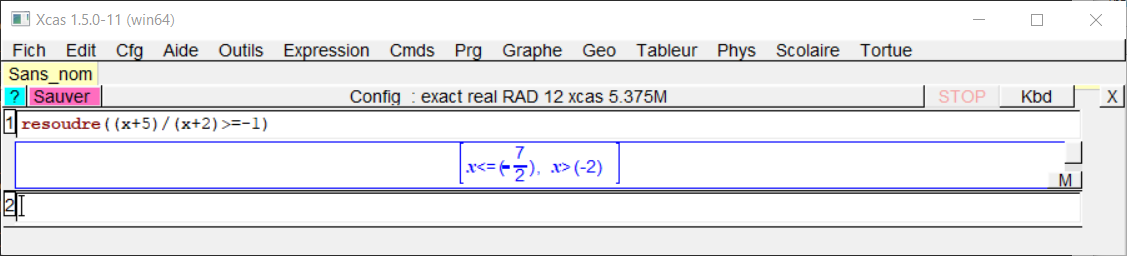
\includegraphics[scale=0.7]{chap03_td_xcas}
\end{center}

\end{document}

\clearpage

\setcounter{numexos}{0}

% !TeX TXS-program:compile = txs:///lualatex

\documentclass[a4paper,11pt]{article}
\usepackage[revgoku]{cp-base}
\graphicspath{{./graphics/}}
%variables
\donnees[%
	classe=1\up{ère} 2M2,matiere={[SPÉ.MATHS]},typedoc=CHAP,numdoc=3,mois=Novembre,annee=2021
]

%formatage
\author{Pierquet}
\title{\nomfichier}
\hypersetup{pdfauthor={Pierquet},pdftitle={\nomfichier},allbordercolors=white,pdfborder=0 0 0,pdfstartview=FitH}
%fancy
\lhead{\entete{\matiere}}
\chead{\entete{\lycee}}
\rhead{\entete{\classe{} - \mois{} \annee}}
%\rhead{\entete{\classe{} - Chapitre }}
\lfoot{\pied{\matiere}}
\cfoot{\logolycee{}}
\rfoot{\pied{\numeropagetot}}

\begin{document}

\pagestyle{fancy}

\part{CH03 - Droites et fonctions affines - Exercices (Correction)}

\smallskip

\exonum{0}%exo1

\begin{enumerate}
	\item La droite $(d)$ est croissante car sa pente ($m=1,5$) est strictement positive.
	\item Le point $A(1~;~7)$ appartient à $(d)$ car $1,5 \times 1 + 5,5 = 7$.
	\item Le point $B(a~;~8)$ appartient à $(d)$ si et seulement si $1,5 \times a+5,5=8$. On résout et on obtient $a=\dfrac53$.
	\item Le point $C(3,5~;~11,5)$ n'appartient pas à $(d)$ car $1,5 \times 3,5 + 5,5 = 10,75 \neq 11,5$.
\end{enumerate}

\medskip

\exonum{1}%exo2


\begin{enumerate}
	\item $f_1(x)=4x-8$ :
	\begin{itemize}
		\item est croissante car $m=4 > 0$ ;
		\item s'annule en $x=2$ ;
		\item est de signe $\ominus0\oplus$.
	\end{itemize}
	\item $f_2(x)=-x+5$ :
	\begin{itemize}
		\item est décroissante car $m=-1 < 0$ ;
		\item s'annule en $x=5$ ;
		\item est de signe $\oplus0\ominus$.
	\end{itemize}
	\item $f_3(x)=3x+5$ :
	\begin{itemize}
		\item est croissante car $m=3 > 0$ ;
		\item s'annule en $x=-\nicefrac{5}{3}$ ;
		\item est de signe $\ominus0\oplus$.
	\end{itemize}
	\item $f_4(x)=-\dfrac23x+\dfrac14$ :
	\begin{itemize}
		\item est décroissante car $m-\nicefrac{2}{3} < 0$ ;
		\item s'annule en $x=\nicefrac{3}{8}$ ;
		\item est de signe $\oplus0\ominus$.
	\end{itemize}
\end{enumerate}

\medskip

\exonum{1}%exo3

\begin{enumerate}
	\item
	\begin{enumerate}
		\item On place les points $A(-1~;~-1)$, $B(1~;~3)$ et $C(2~;~2)$ :
		\begin{center}
			\begin{tikzpicture}[x=0.7cm,y=0.7cm,xmin=-2,xmax=4,ymin=-2,ymax=4]
				\tgrillep \axestikz* \axextikz*{-2,-1,...,3} \axeytikz*{-2,-1,...,3}
				\clip (\xmin,\ymin) rectangle (\xmax,\ymax) ;
				\draw[ultra thick,red,domain=\xmin:\xmax,samples=2] plot (\x,{2*\x+1}) ;
				\draw[ultra thick,blue,domain=\xmin:\xmax,samples=2] plot (\x,{\x}) ;
				\draw[ultra thick,ForestGreen,domain=\xmin:\xmax,samples=2] plot (\x,{-\x+4}) ;
				\foreach \Point/\Nom/\Pos in {(-1,-1)/A/above left,(1,3)/B/left,(2,2)/C/right}
					\filldraw \Point circle[radius=2pt] node[\Pos] {\Large \point{\Nom}} ;
			\end{tikzpicture}
		\end{center}
		\item On lit -- graphiquement (!) -- que :
		\begin{itemize}
			\item $(AB)$ : $y=2x+1$ ;
			\item $(AC)$ : $y=x$ ;
			\item $(BC)$ : $y=-x+4$.
		\end{itemize}
	\end{enumerate}
	\item Par lectures graphiques :
	\begin{itemize}
		\item $(d_1)$ : $y=-x+2$ ;
		\item $(d_2)$ : $y=3x-1$ ;
		\item $(d_3)$ : $y=y=2$ ;
		\item $(d_4)$ : $y=0,8x-2$ ;
		\item $(d_5)$ : $x=4$ ;
		\item $(d_6)$ : $y=30x-20$ ;
		\item $(d_7)$ : $y=-\tfrac{10}{3}x+80$ ;
		\item $(d_8)$ : $y=4x$.
	\end{itemize}
\end{enumerate}

\medskip

\exonum{2}%exo4

\begin{enumerate}
	\item Par \uline{calculs} :
	\begin{itemize}
		\item $m=\dfrac{DV}{DH}=\dfrac{y_L-y_K}{x_L-x_K}=\dfrac{65,47-15,75}{100,4-10}=0,55$ ;
		\item ainsi $(KL)$ : $y=0,55x+p$ ;
		\item avec $K$, on obtient $0,55 \times 10 + p = 15,75 \Rightarrow p = 15,75 - 0,55 \times 10 = 10,25$.
	\end{itemize}
	Ainsi on obtient $(KL)$ : $y=0,55x+10,25$.
	\item Le point de coordonnées $(50\,;\,37,85)$ n'appartient pas à la droite $(KL)$ car $0,55 \times 50 + 10,25 = 37,74 \neq 37,85$.
\end{enumerate}

\medskip

\exonum{1}%exo5

\begin{enumerate}
	\item
	\begin{enumerate}
		\item Le coefficient directeur de $(AB)$ vaut $m_{(AB)}=\dfrac{y_B-y_A}{x_B-x_A}=\dfrac{8-2}{2-1}=6$.
		\item Le coefficient directeur de la droite $(AC)$ est $m_{(AC)}=\dfrac{y_C-y_A}{x_C-x_A}=\dfrac{26-2}{5-1}=6$.
		\item Une équation de $(AB)$ est $y=6x-4$ (car $p=2-6\times1$).
	\end{enumerate}
	\item On va regarder si $C$ appartient à la droite $(AB)$ : $6 \times 5 - 4 = 26$ $\checkmark$.
	
	Donc les points $A$, $B$ et $C$ sont bien alignés.
\end{enumerate}

\medskip

\exonum{3}%exo6

\begin{enumerate}
	\item Les expressions suivantes sont bien sous forme de produit(s)/quotient(s), donc tds ok :
	\begin{enumerate}
		\item $(x-3)(2x-4)$ :
		\begin{center}
			\begin{tikzpicture}
				\tkzTabInit[]{$x$/0.8,$(x-3)$/0.8,$(2x-4)$/0.8,expr/0.8}{$-\infty$, $2$, $3$, $+\infty$}
				\draw[] (T21) -- (T22) node [midway, right] {$\: m=1 \: \oplus$};
				\draw[] (T22) -- (T23) node [midway, right] {$\: m=2 \: \oplus$};
				\tkzTabLine{,-,t,-,z,+,}
				\tkzTabLine{,-,z,+,t,+,}
				\tkzTabLine{,+,z,-,z,+,}
			\end{tikzpicture}
			
			\smallskip
			
			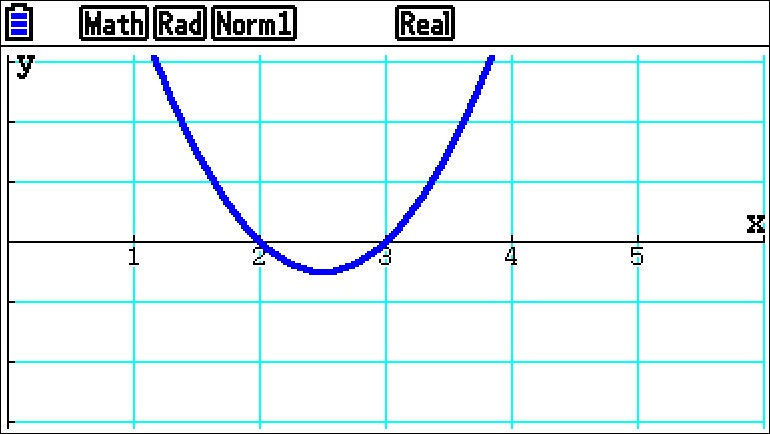
\includegraphics[width=4.5cm]{chap03_corr_exo6_a}
			
			\pagebreak
		\end{center}
		\item $-x(3x+4)$ :
		\begin{center}
			\begin{tikzpicture}
				\tkzTabInit[]{$x$/0.8,$-x$/0.8,$(3x+4)$/0.8,expr/0.8}{$-\infty$, $-\nicefrac{4}{3}$, $0$, $+\infty$}
				\draw[] (T21) -- (T22) node [midway, right] {$\: m=-1 \: \ominus$};
				\draw[] (T22) -- (T23) node [midway, right] {$\: m=3 \: \oplus$};
				\tkzTabLine{,+,t,+,z,-,}
				\tkzTabLine{,-,z,+,t,+,}
				\tkzTabLine{,-,z,+,z,-,}
			\end{tikzpicture}
			
			\smallskip
			
			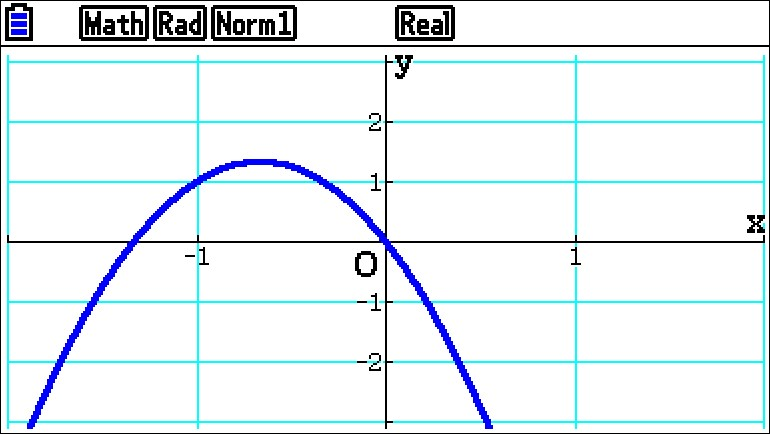
\includegraphics[width=4.5cm]{chap03_corr_exo6_b}
		\end{center}
		\item $(x-2)(x+5)(7-7x)$ :
		\begin{center}
			\begin{tikzpicture}
				\tkzTabInit[espcl=2.5]{$x$/0.8,$(x-2)$/0.8,$(x+5)$/0.8,$(7-7x)$/0.8,expr/0.8}{$-\infty$, $-5$, $1$,$2$,$+\infty$}
				\draw[] (T21) -- (T22) node [midway, right] {$\: m=1 \: \oplus$};
				\draw[] (T22) -- (T23) node [midway, right] {$\: m=1 \: \oplus$};
				\draw[] (T23) -- (T24) node [midway, right] {$\: m=-7 \: \ominus$};
				\tkzTabLine{,-,t,-,t,-,z,+,}
				\tkzTabLine{,-,z,+,t,+,t,+,}
				\tkzTabLine{,+,t,+,z,-,t,-,}
				\tkzTabLine{,+,z,-,z,+,z,-,}
			\end{tikzpicture}
			
			\smallskip
			
			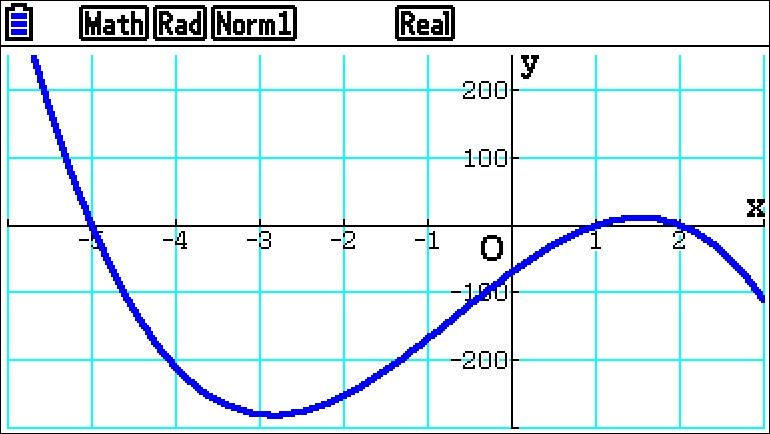
\includegraphics[width=4.5cm]{chap03_corr_exo6_c}
		\end{center}
		\item $\dfrac{2x+1}{(x-5)(x-1)}$ :
		\begin{center}
			\begin{tikzpicture}[double distance=3]
				\tkzTabInit[espcl=2.5]{$x$/0.8,$(2x+1)$/0.8,$(x-5)$/0.8,$(x-1)$/0.8,expr/0.8}{$-\infty$, ${-0,5}$, $1$,$5$,$+\infty$}
				\draw[] (T21) -- (T22) node [midway, right] {$\: m=2 \: \oplus$};
				\draw[] (T22) -- (T23) node [midway, right] {$\: m=1 \: \oplus$};
				\draw[] (T23) -- (T24) node [midway, right] {$\: m=1 \: \oplus$};
				\draw(N31) node [yshift=3pt] {{\scriptsize \red \textsf{D}}};
				\draw(N41) node [yshift=3pt] {{\scriptsize \red \textsf{D}}};
				\tkzTabLine{,-,z,+,t,+,t,+,}
				\tkzTabLine{,-,t,-,t,-,z,+,}
				\tkzTabLine{,-,t,-,z,+,t,+,}
				\tkzTabLine{,-,z,+,d,-,d,+,}
			\end{tikzpicture}
			
			\smallskip
			
			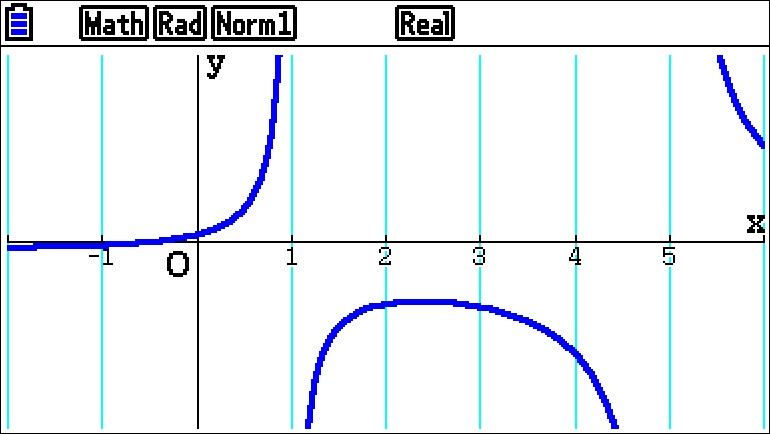
\includegraphics[width=4.5cm]{chap03_corr_exo6_d}
		\end{center}
		
		\pagebreak
		\item $\dfrac{-7(x+2)}{5-2x}$ :
		\begin{center}
			\begin{tikzpicture}[double distance=3]
				\tkzTabInit[]{$x$/0.8,$-7$/0.8,$(x+2)$/0.8,$(5-2x)$/0.8,expr/0.8}{$-\infty$, ${-2}$, ${2,5}$,$+\infty$}
				\draw[] (T22) -- (T23) node [midway, right] {$\: m=1 \: \oplus$};
				\draw[] (T23) -- (T24) node [midway, right] {$\: m=-2 \: \ominus$};
				\draw(N31) node [yshift=3pt] {{\scriptsize \red \textsf{D}}};
				\tkzTabLine{,-,t,-,t,-,}
				\tkzTabLine{,-,z,+,t,+,}
				\tkzTabLine{,+,t,+,z,-,}
				\tkzTabLine{,+,z,-,d,+,}
			\end{tikzpicture}
			
			\smallskip
			
			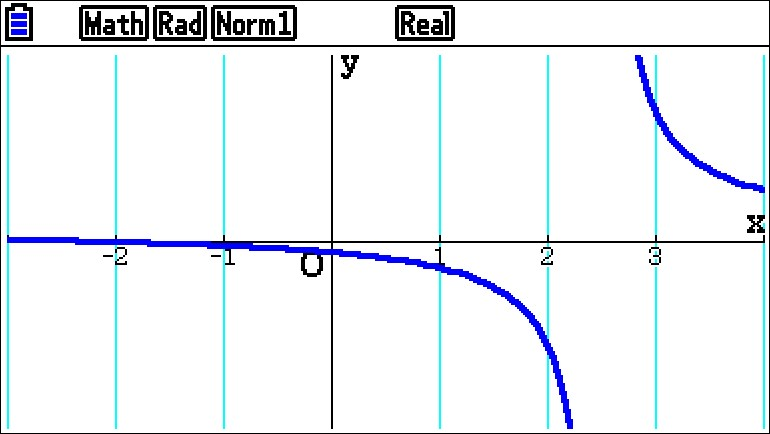
\includegraphics[width=4.5cm]{chap03_corr_exo6_e}
		\end{center}
		\item $\dfrac{x^2+3}{(x-1)(x+4)}$ :
		\begin{center}
			\begin{tikzpicture}[double distance=3]
				\tkzTabInit[]{$x$/0.8,$(x^2+3)$/0.8,$(x-1)$/0.8,$(x+4)$/0.8,expr/0.8}{$-\infty$, ${-4}$, ${1}$,$+\infty$}
				\draw[] (T22) -- (T23) node [midway, right] {$\: m=1 \: \oplus$};
				\draw[] (T23) -- (T24) node [midway, right] {$\: m=1 \: \oplus$};
				\draw(N21) node [yshift=3pt] {{\scriptsize \red \textsf{D}}};
				\draw(N31) node [yshift=3pt] {{\scriptsize \red \textsf{D}}};
				\tkzTabLine{,+,t,+,t,+,}
				\tkzTabLine{,-,t,-,z,+,}
				\tkzTabLine{,-,z,+,t,-,}
				\tkzTabLine{,+,d,-,d,+,}
			\end{tikzpicture}
			
			\smallskip
			
			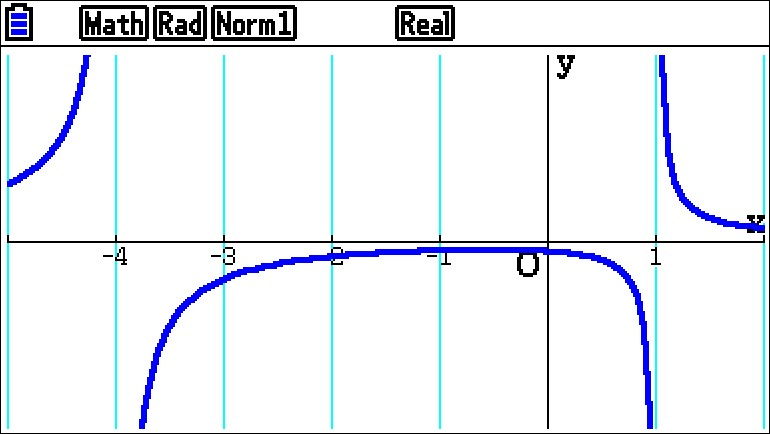
\includegraphics[width=4.5cm]{chap03_corr_exo6_f}
		\end{center}
	\end{enumerate}
	\item On utilise, ci-besoin, les techniques habituelles pour transformer
	\begin{enumerate}
		\item $(x-3)(x-1) -2(x-3)(4x-7) = (x-3)\left[ (x-1)-2(4x-7)\right] = (x-3)(x-1-8x+14)=(x-3)(-7x+13)$ :
		\begin{center}
			\begin{tikzpicture}
				\tkzTabInit[lgt=2.5]{$x$/0.8,$(x-3)$/0.8,$(-7x+13)$/0.8,expr/0.8}{$-\infty$, $\nicefrac{13}{7}$, $3$, $+\infty$}
				\draw[] (T21) -- (T22) node [midway, right] {$\: m=1 \: \oplus$};
				\draw[] (T22) -- (T23) node [midway, right] {$\: m=-7 \: \ominus$};
				\tkzTabLine{,-,t,-,z,+,}
				\tkzTabLine{,+,z,-,t,-,}
				\tkzTabLine{,-,z,+,z,-,}
			\end{tikzpicture}
			
			\smallskip
			
			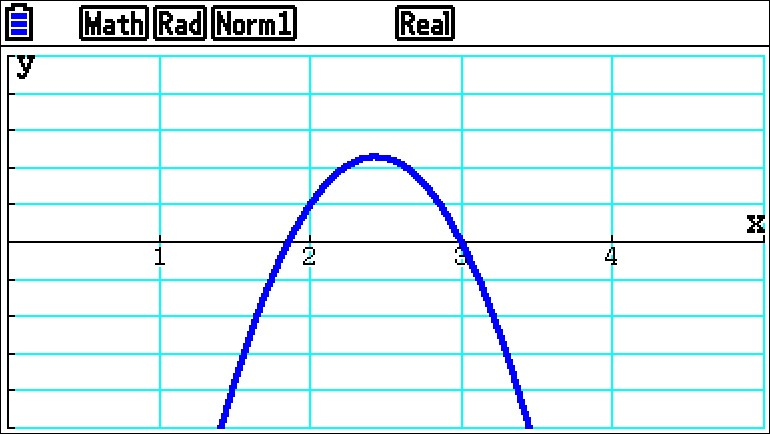
\includegraphics[width=4.5cm]{chap03_corr_exo6_g}
		\end{center}
		
		\pagebreak 
		\item $3-\dfrac{5+x}{7x-13} = \dfrac{3(7x-13)}{7x-13} - \dfrac{5+x}{7x-13} = \dfrac{21x-39-5-x}{7x-13} = \dfrac{20x-44}{7x-13}$ :
		\begin{center}
			\begin{tikzpicture}[double distance=3]
				\tkzTabInit[lgt=2.5]{$x$/0.8,$(20x-44)$/0.8,$(7x-13)$/0.8,expr/0.8}{$-\infty$, $\nicefrac{13}{7}$, $\nicefrac{11}{5}$, $+\infty$}
				\draw[] (T21) -- (T22) node [midway, right] {$\: m=20 \: \oplus$};
				\draw[] (T22) -- (T23) node [midway, right] {$\: m=7 \: \oplus$};
				\draw(N21) node [yshift=3pt] {{\scriptsize \red \textsf{D}}};
				\tkzTabLine{,-,t,-,z,+,}
				\tkzTabLine{,-,z,+,t,+,}
				\tkzTabLine{,+,d,-,z,+,}
			\end{tikzpicture}
			
			\smallskip
			
			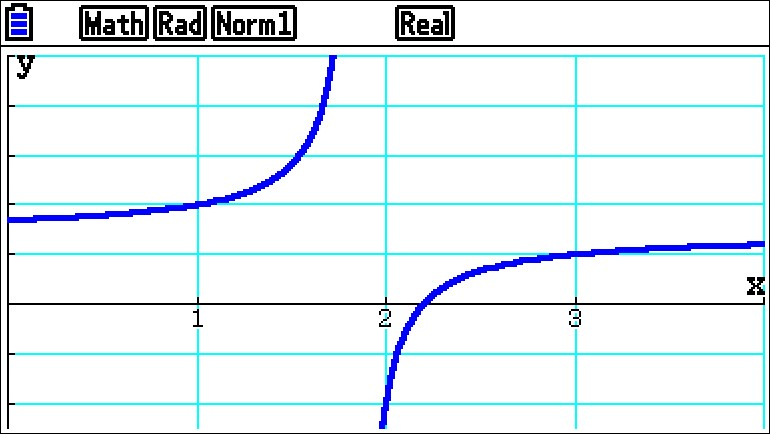
\includegraphics[width=4.5cm]{chap03_corr_exo6_h}
		\end{center}
		\item $x(x+2)(x-3)^2 = x(x+2)(x-3)(x-3)$ :
		\begin{center}
			\begin{tikzpicture}[]
				\tkzTabInit[espcl=2.75]{$x$/0.8,$x$/0.8,$(x+2)$/0.8,$(x-3)$/0.8,$(x-3)$/0.8,expr/0.8}{$-\infty$, ${-2}$, ${0}$,$3$,$+\infty$}
				\draw[] (T21) -- (T22) node [midway, right] {$\: m=1 \: \oplus$};
				\draw[] (T22) -- (T23) node [midway, right] {$\: m=1 \: \oplus$};
				\draw[] (T23) -- (T24) node [midway, right] {$\: m=1 \: \oplus$};
				\draw[] (T24) -- (T25) node [midway, right] {$\: m=1 \: \oplus$};
				\tkzTabLine{,-,t,-,z,+,t,+,}
				\tkzTabLine{,-,z,+,t,+,t,+,}
				\tkzTabLine{,-,t,-,t,-,z,+,}
				\tkzTabLine{,-,t,-,t,-,z,+,}
				\tkzTabLine{,+,z,-,z,+,z,+,}
			\end{tikzpicture}
			
			\smallskip
			
			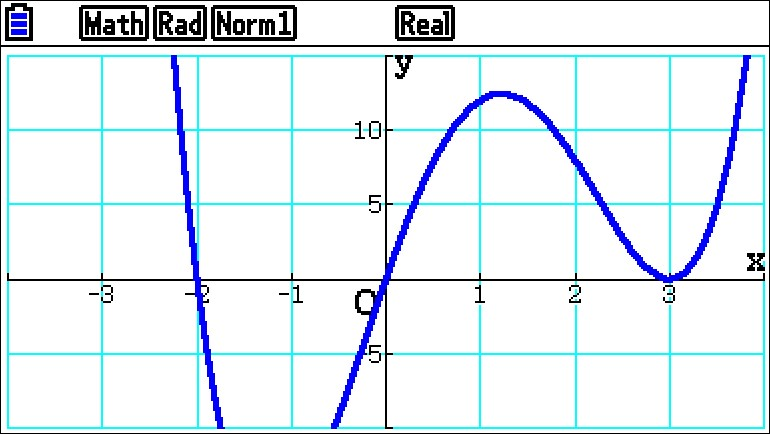
\includegraphics[width=4.5cm]{chap03_corr_exo6_i}
		\end{center}
	\end{enumerate}
\end{enumerate}

\medskip

\exonum{3}%exo7

\begin{enumerate}
	\item On peut résoudre, à l'aide d'un tds :
	\begin{enumerate}
		\item $(x-3)(2x+4) \pg 0$  donne $\mathscr{S} = \intervOF{\strut-\infty}{-2} \cup \intervFO{3}{\strut+\infty}$.
		\item $3x(x+1)(7+x) < 0$ donne $\mathscr{S} = \intervOO{\strut-\infty}{-7} \cup \intervOO{-1}{\strut 0}$.
		\item $\dfrac{x+3}{2x+8} \pp 0$ donne $\mathscr{S} = \intervOF{\strut-4}{-3}$.
		\item $\dfrac{x(x+2)}{x+1} > 0$ donne $\mathscr{S} = \intervOO{\strut-2}{-1} \cup \intervOO{0}{\strut+\infty}$.
	\end{enumerate}
	\item En utilisant les techniques de \textit{transformation}, on transforme pour pouvoir réaliser un tds :
	\begin{enumerate}
		\item $7x+3 \pp 2 \ssi 7x+1 \pp 0$ donne $\mathscr{S} = \intervOO{-\infty}{\strut-\tfrac{1}{7}}$.
		\item $(x+1)(x-2) < (x+1)(4x+5) \ssi (x+1)(x-2)-(x+1)(4x-5) < 0 \ssi (x+1)(x-2-4x-5) < 0$.
		
		Et $(x+1)(-3x-7) < 0$ donne $\mathscr{S} = \intervOO{\strut-\infty}{-\tfrac{7}{3}} \cup \intervOO{-1}{\strut+\infty}$.
		\item $\dfrac{x+1}{x+2} < 2 \ssi \dfrac{x+1}{x+2} - 2 < 0 \ssi \dfrac{x+1}{x+2} - \dfrac{2(x+2)}{x+2} < 0 \ssi \dfrac{x+1-2(x+2)}{x+2} < 0 \ssi \dfrac{-x-3}{x+2} < 0$.
		
		Et $\dfrac{-x-3}{x+2} < 0$ donne $\mathscr{S} = \intervOO{\strut-\infty}{-3} \cup \intervOO{-2}{\strut+\infty}$.
	\end{enumerate}
\end{enumerate}
\begin{center}
	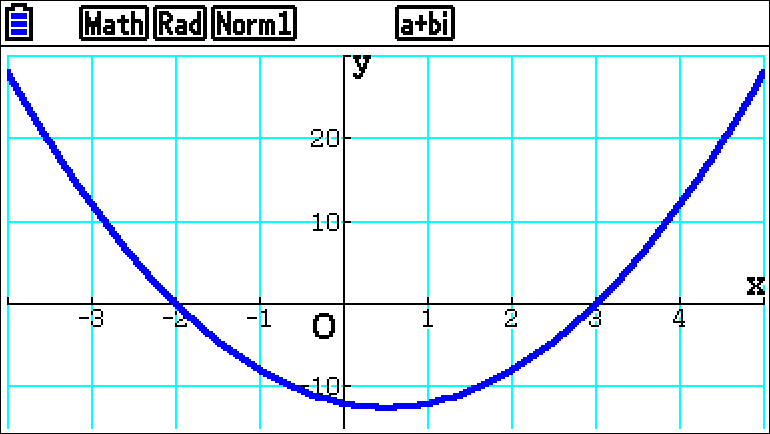
\includegraphics[width=4.5cm]{chap03_corr_exo7_a}~~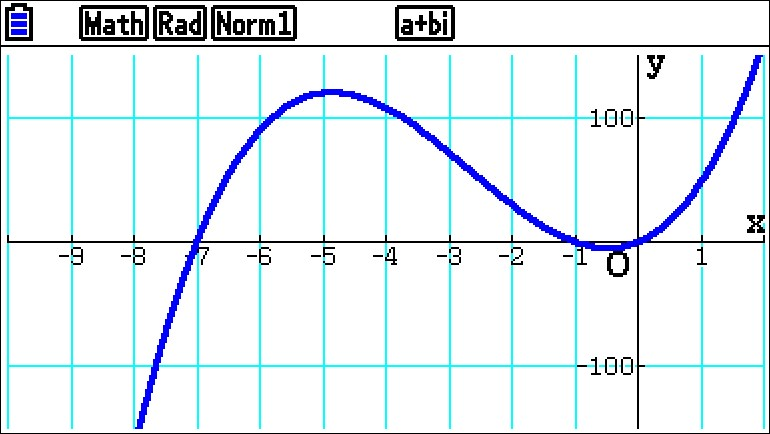
\includegraphics[width=4.5cm]{chap03_corr_exo7_b}~~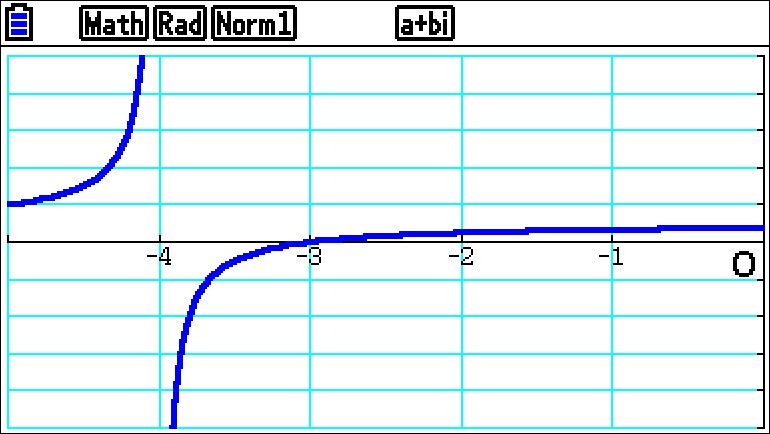
\includegraphics[width=4.5cm]{chap03_corr_exo7_c}~~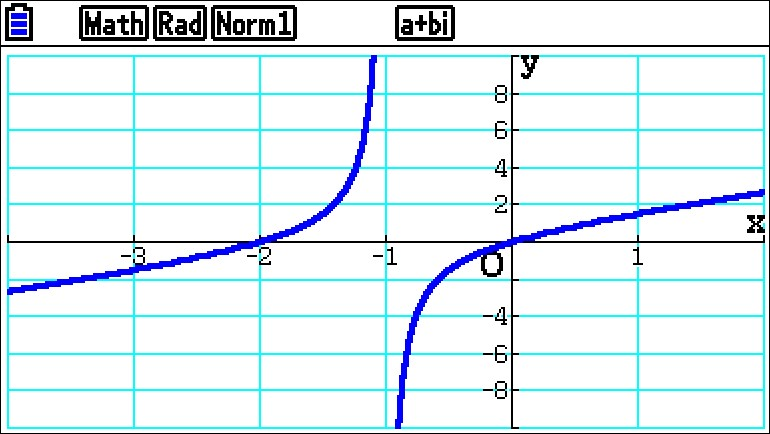
\includegraphics[width=4.5cm]{chap03_corr_exo7_d}
\end{center}
\begin{center}
	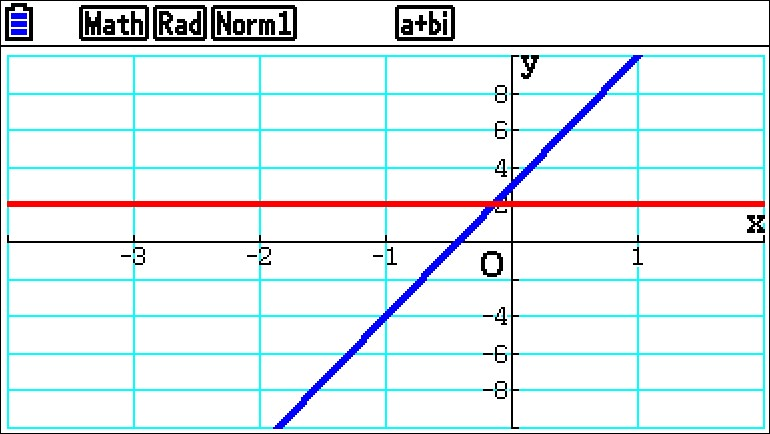
\includegraphics[width=4.5cm]{chap03_corr_exo7_e}~~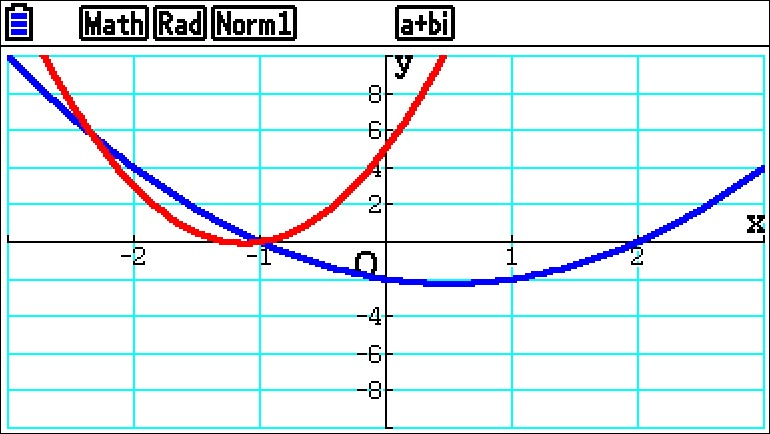
\includegraphics[width=4.5cm]{chap03_corr_exo7_f}~~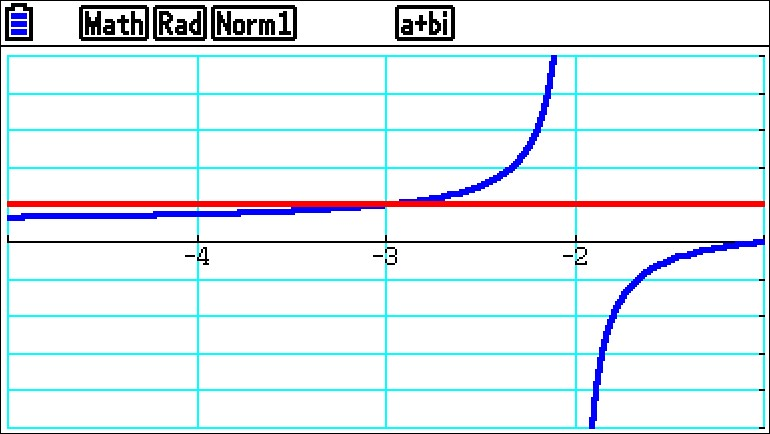
\includegraphics[width=4.5cm]{chap03_corr_exo7_g}
\end{center}

\medskip

\exonum{3}%exo8

\medskip

Le logiciel \cxcas{Xcas} nous donne les solutions de l'inéquation $\dfrac{x+5}{x+2} \pg -1$, qui sont $\intervOF{-\infty}{-\dfrac{7}{2}} \cup \intervOO{-2}{+\infty}$, en effet :

\begin{itemize}
	\item $\dfrac{x+5}{x+2} \pg 1 \ssi \dfrac{x+5}{x+2}+1 \pg 0 \ssi \dfrac{x+5}{x+2}+\dfrac{x+2}{x+2} \pg 0 \ssi \dfrac{2x+7}{x+2} \pg 0$ (\textsf{ZPQ} $\checkmark$)
	\smallskip
	\item $2x+7=0 \ssi x=-\tfrac72$ et $x+2=0 \ssi x=-2$
	
	\begin{center}
		\begin{tikzpicture}[double distance=3]
			\tkzTabInit[lgt=2.5]{$x$/0.8,$(x+5)$/0.8,$(x+2)$/0.8,expr/0.8}{$-\infty$, $\nicefrac{-7}{2}$, $-2$, $+\infty$}
			\draw[] (T21) -- (T22) node [midway, right] {$\: m=1 \: \oplus$};
			\draw[] (T22) -- (T23) node [midway, right] {$\: m=1 \: \oplus$};
			\draw(N31) node [yshift=3pt] {{\scriptsize \red \textsf{D}}};
			\tkzTabLine{,-,z,-,t,+,}
			\tkzTabLine{,-,t,+,z,+,}
			\tkzTabLine{,+,z,-,d,+,}
		\end{tikzpicture}
	\end{center}
	\begin{center}
		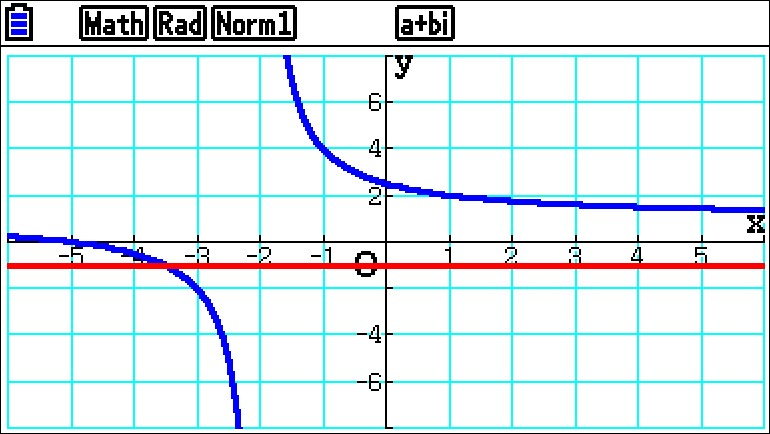
\includegraphics[width=4.5cm]{chap03_corr_exo8}
	\end{center}
\end{itemize}

\end{document}

\clearpage

% !TeX TXS-program:compile = txs:///pythonlualatex

\documentclass[a4paper,11pt]{article}
\usepackage[breakable,pythontex]{cp-base}
\graphicspath{{./graphics/}}
%variables
\donnees[typedoc=CHAPITRE~,numdoc=4,classe=1\up{ère} 2M2,matiere={[SPÉ.MATHS]},annee=2021]

%formatage
\author{Pierquet}
\title{\nomfichier}
\hypersetup{pdfauthor={Pierquet},pdftitle={\nomfichier},allbordercolors=white,pdfborder=0 0 0,pdfstartview=FitH}
%divers
\lhead{\entete{\matiere}}
\chead{\entete{\lycee}}
\rhead{\entete{\classe{} - Chapitre \thepart}}
\lfoot{\pied{\matiere}}
\cfoot{\logolycee{}}
\rfoot{\pied{\numeropagetot}}

\begin{document}

\pagestyle{fancy}

\part{CH04 - Second degré, études de signes}

\section{Signe d'une fonction du second degré}

\subsection{Idée}

\begin{cidee}
Dans le chapitre 1, on a vu que le polynôme du second degré $ax^2+bx+c$ peut (éventuellement) se factoriser sous forme d'un produit de facteurs du premier degré. Les rappels vus au chapitre 3 permettent désormais de déterminer le signe d'un trinôme !
\end{cidee}

\subsection{Le théorème}

\begin{cthm}
Un polynôme du second degré $ax^2+bx+c$ ($a \neq 0$) est du signe de $a$, sauf entre les racines quand elles existent.
\end{cthm}

\begin{cdemo}
Soit $f$ une fonction du second degré, définie sur $\R$ par $f(x)=ax^2+bx+c$ avec $a\ne0$. On sait que le nombre de racines de cette fonction (le nombre de zéros dans le tableau de signes) dépend du signe de $\Delta=b^2-4ac$. \vspace{-0.1cm}
\begin{description}
	\item[Lorsque $\Delta$ est positif,] on sait que le polynôme possède deux racines $x_1$ et $x_2$ et qu'on peut le factoriser sous la forme $f(x)=a(x-x_1)(x-x_2)$. Le signe de $f$ peut alors être déterminé grâce à la règle des signes ! \vspace{-0.15cm}
	\begin{center}
		\begin{tikzpicture}
			\tkzTabInit[lgt=3.5]{$x$ / 0.6 , $a$ / 0.6 , $x-x_1$ / 0.6 , $x-x_2$ / 0.6 , produit $f(x)$ / 0.6}{$-\infty$, $x_1$, $x_2$, $+\infty$}
			\tkzTabLine{, , , \text{signe de }a , , ,}
			\tkzTabLine{,- ,z , ,+ , ,}
			\tkzTabLine{, ,- , ,z , +,}
			\tkzTabLine{,\text{signe de }a , z, \text{signe de }-a ,z ,\text{signe de }a ,}
		\end{tikzpicture}
	\end{center}
	\item[Lorsque $\Delta$ est nul,] on sait que le polynôme possède une unique racines $\alpha$ et  et qu'on peut le factoriser sous la forme $f(x)=a(x-\alpha)^2$. Le signe de $f$ peut alors aussi être déterminé grâce à la règle des signes !  \vspace{-0.15cm}
	\begin{center}
		\begin{tikzpicture}
			\tkzTabInit[lgt=3.5]{$x$ / 0.6 , $a$ / 0.6 , $x-\alpha$ / 0.6 , $x-\alpha$ / 0.6 , produit $f(x)$ / 0.6}{$-\infty$, $\alpha$, $+\infty$}
			\tkzTabLine{, , \text{signe de }a , ,}
			\tkzTabLine{,- ,z ,+ , }
			\tkzTabLine{,- ,z , +,}
			\tkzTabLine{,\text{signe de }a , z ,\text{signe de }a ,}
		\end{tikzpicture}
	\end{center}
	\item[Lorsque $\Delta$ est négatif,] le polynôme n'a pas de racine, on ne peut pas le factoriser. La parabole ne traverse jamais l'axe des abscisses, donc elle est toujours de même signe. \\Si $a>0$, la parabole est ouverte vers le haut. Comme l'axe des abscisses ne la traverse pas, c'est qu'il passe en dessous. Donc la fonction est toujours positive comme $a$. \\ Si $a<0$, la parabole est ouverte vers le bas et n'est pas traversée par l'axe des abscisses, donc elle doit être située en-dessous de celui-ci et la fonction est toujours négative, comme $a$. \vspace{-0.15cm}
	\begin{center}
		\begin{tikzpicture}
			\tkzTabInit{$x$ / 0.6 ,  $f(x)$ / 0.6}{$-\infty$,  $+\infty$}
			\tkzTabLine{ , \text{signe de }a ,}
		\end{tikzpicture}
	\end{center}	
\end{description}
\end{cdemo}

\begin{calgo}
En \calgpython, on peut créer une \calg{fonction} et une \calg{procédure} permettant d'afficher le signe de $ax^2+bx+c$ :

\begin{tcpythoncode}[15cm]
	\begin{pyverbatim}[][fontsize=\footnotesize,numbers=left,numbersep=10pt]
		from math import *
		#les racines
		def racines(a,b,c):
			delta = b**2 - 4*a*c
			if delta > 0:
				return (-b+sqrt(delta))/(2*a),(-b-sqrt(delta))/(2*a)
			elif delta == 0:
				return -b/(2*a)
		#le signe
		def signe(a,b,c):
			delta = b**2 - 4*a*c
			if delta > 0 :
				print(f"Les racines sont {racines(a,b,c)}")
				if a>0 : print(f"Le signe du trinôme est +0-0+")
				else : print(f"Le signe du trinôme est -0+0-")
			elif delta == 0:
				print(f"La racine est {racines(a,b,c)}")
				if a>0 : print(f"Le signe du trinôme est +0+")
				else : print(f"Le signe du trinôme est -0-")
			else :
				print(f"Pas de racine")
				if a>0 : print(f"Le signe du trinôme est +")
				else : print(f"Le signe du trinôme est -")
	\end{pyverbatim}
\end{tcpythoncode}

\begin{pyconcode}
from math import *
def racines(a,b,c):
	delta = b**2 - 4*a*c
	if delta > 0:
		return (-b+sqrt(delta))/(2*a),(-b-sqrt(delta))/(2*a)
	elif delta == 0:
		return -b/(2*a)
	

def signe(a,b,c):
	delta = b**2 - 4*a*c
	if delta > 0:
		print(f"Les racines sont {racines(a,b,c)}")
		if a>0:
			print(f"Le signe du trinôme est +0-0+")
		else :
			print(f"Le signe du trinôme est -0+0-")
	elif delta == 0:
		print(f"La racine est {racines(a,b,c)}")
		if a>0:
			print(f"Le signe du trinôme est +0+")
		else :
			print(f"Le signe du trinôme est -0-")
	else :
		print(f"Pas de racine")
		if a>0:
			print(f"Le signe du trinôme est +")
		else :
			print(f"Le signe du trinôme est -")


\end{pyconcode}

\begin{consolepython}[15cm]
\begin{pyconsole}[][framesep=3mm,frame=single,label={[\scriptsize Début de la console \logopython]\scriptsize Fin de la console \logopython},fontsize=\footnotesize,framerule=1pt,rulecolor=\color{ForestGreen}]
signe(1,5,6)
signe(1,1,1)
signe(-1,-6,-9)
\end{pyconsole}
\end{consolepython}
\smallskip
\end{calgo}

\begin{cillustr}
En pratique, il suffit de connaître les éventuelles racines du polynôme et de regarder le signe de $a$ pour visualiser la parabole et donc obtenir le tableau de signes !	
\begin{center}
	\tunits{0.5}{0.5}
	\tdefgrille{-3}{3}{1}{0.5}{-3}{3}{1}{0.5}
	\begin{tikzpicture}[x=\xunit cm,y=\yunit cm]
		%\tgrilles ;
		\axestikz* ;
		\draw (0,-3.25) node {{\red $a>0$} et {\blue $\Delta>0$}} ;
		\clip (\xmin,\ymin) rectangle (\xmax,\ymax) ;
		\draw[line width=1.25pt,red,domain=-3:3,samples=200] plot (\x,{(\x-1)*(\x+2)}) ; 
	\end{tikzpicture}
	\hspace{0.5cm}
	\tdefgrille{-3}{3}{1}{0.5}{-1}{5}{1}{0.5}
	\begin{tikzpicture}[x=\xunit cm,y=\yunit cm]
		%\tgrilles ;
		\axestikz* ;
		\draw (0,-1.25) node {{\red $a>0$} et {\blue $\Delta=0$}} ;
		\clip (\xmin,\ymin) rectangle (\xmax,\ymax) ;
		\draw[line width=1.25pt,red,domain=-3:3,samples=200] plot (\x,{0.5*(\x-0.5)*(\x-0.5)}) ; 
	\end{tikzpicture}
	\hspace{0.5cm}
	\tdefgrille{-3}{3}{1}{0.5}{-1}{5}{1}{0.5}
	\begin{tikzpicture}[x=\xunit cm,y=\yunit cm]
		%\tgrilles ;
		\axestikz* ;
		\draw (0,-1.25) node {{\red $a>0$} et {\blue $\Delta<0$}} ;
		\clip (\xmin,\ymin) rectangle (\xmax,\ymax) ;
		\draw[line width=1.25pt,red,domain=-3:3,samples=200] plot (\x,{(\x+1)*(\x+1)+0.5}) ; 
	\end{tikzpicture}

	\smallskip
	
	\tdefgrille{-3}{3}{1}{0.5}{-3}{3}{1}{0.5}
	\begin{tikzpicture}[x=\xunit cm,y=\yunit cm]
		%\tgrilles ;
		\axestikz* ;
		\draw (0,-3.25) node {{\green $a<0$} et {\blue $\Delta>0$}} ;
		\clip (\xmin,\ymin) rectangle (\xmax,\ymax) ;
		\draw[line width=1.25pt,green,domain=-3:3,samples=200] plot (\x,{-(\x-1)*(\x+2)}) ; 
	\end{tikzpicture}
	\hspace{0.5cm}
	\tdefgrille{-3}{3}{1}{0.5}{-5}{1}{1}{0.5}
	\begin{tikzpicture}[x=\xunit cm,y=\yunit cm]
		%\tgrilles ;
		\axestikz* ;
		\draw (0,-5.25) node {{\green $a<0$} et {\blue $\Delta=0$}} ;
		\clip (\xmin,\ymin) rectangle (\xmax,\ymax) ;
		\draw[line width=1.25pt,green,domain=-3:3,samples=200] plot (\x,{-0.5*(\x-0.5)*(\x-0.5)}) ; 
	\end{tikzpicture}
	\hspace{0.5cm}
	\tdefgrille{-3}{3}{1}{0.5}{-5}{1}{1}{0.5}
	\begin{tikzpicture}[x=\xunit cm,y=\yunit cm]
		%\tgrilles ;
		\axestikz* ;
		\draw (0,-5.25) node {{\green $a<0$} et {\blue $\Delta<0$}} ;
		\clip (\xmin,\ymin) rectangle (\xmax,\ymax) ;
		\draw[line width=1.25pt,green,domain=-3:3,samples=200] plot (\x,{-(\x+1)*(\x+1)-0.5}) ; 
	\end{tikzpicture}
\end{center}

\end{cillustr}

\section{Résolution d'inéquations}

\subsection{Cas du second degré}

\begin{cmethode}
Pour résoudre une inéquation \textbf{du second degré}, on utilise un tableau de signes :
\begin{itemize}
	\item on se ramène à une étude de signes en passant tout du même côté de l'inégalité ;
	\item on dresse le tableau de signes de l'expression obtenue ;
	\item on y lit l'ensemble des solutions.
\end{itemize}
\end{cmethode}

\subsection{Cas général}

\begin{cmethode}
Pour résoudre une inéquation, l'outil le plus efficace est très souvent le tableau de signes, après avoir tout passé du même côté.

\smallskip

Il est parfois nécessaire de \textbf{transformer} l'expression obtenue pour pouvoir dresser son tableau de signes facilement. On a vu dans ce chapitre et le précédent comment étudier le signe d'une fonction affine et d'un polynôme du second degré. Si une autre forme se présente, il peut être nécessaire de :
\begin{itemize}
	\item reconnaître une expression qui est toujours de même signe (carré, racine, somme de nombres positifs, somme de nombres négatifs, \ldots) ;
	\item factoriser l'expression, pour étudier le signe de chacun des facteurs avant d'utiliser la règle des signes ;
	\item écrire l'expression sous forme d'un quotient (mettre au même dénominateur), pour étudier le signe du numérateur puis du dénominateur avant d'utiliser là encore la règle des signes.
\end{itemize}
\end{cmethode}

\begin{cidee}
On peut retenir ce principe sous le \og petit \fg{} nom de \textsf{méthode ZPQ}.
\end{cidee}

\begin{cattention}
Il ne faut \textbf{jamais} découper une expression en étudiant le signe de chaque terme d'une somme (ou d'une différence) dans un tableau, car c'est la règle des signes ($\times$, $\div$) qui est à la base des tableaux de signes !
\end{cattention}

\section{Position relative de deux courbes}

\begin{cdefi}
Étudier la \textbf{position relative} de deux courbes, c'est déterminer laquelle est graphiquement située au-dessus de l'autre. Cela peut varier suivant les intervalles.
\end{cdefi}

\begin{cmethode}
Soient $f$ et $g$ deux fonctions définies sur $\R$. Pour étudier la position relative de $\mathscr{C}_f$ et $\mathscr{C}_g$ :
\begin{itemize}
	\item on calcule la différence $f(x)-g(x)$ ;
	\item on étudie son signe dans un tableau ;
	\item on conclut : sur les intervalles où la différence est positive, c'est $\mathscr{C}_f$ qui est au-dessus, et inversement.
\end{itemize}
\end{cmethode}

\begin{cexemple}[s]
Déterminer la position relative de la parabole $\mathscr{P}$ d'équation $y=0,5x^2+2x-4$ et de la droite $\mathscr{D}$ d'équation $y=3x-2,5$.

Mêmes questions avec la parabole $\mathscr{P}$ d'équation $y=x^2-5x+3$ et la droite $\mathscr{D}$ d'équation $y=12x-69$.
\end{cexemple}

\end{document}

\clearpage

\setcounter{numexos}{0}

% !TeX TXS-program:compile = txs:///lualatex

\documentclass[a4paper,11pt]{article}
\usepackage[revgoku]{cp-base}
\graphicspath{{./graphics/}}
%variables
\donnees[%
	classe={1\up{ère} 2M2},matiere={[SPÉ.MATHS]},mois=Novembre,annee=2021,typedoc=CHAP,numdoc=4]

%formatage
\author{Pierquet}
\title{\nomfichier}
\hypersetup{pdfauthor={Pierquet},pdftitle={\nomfichier},allbordercolors=white,pdfborder=0 0 0,pdfstartview=FitH}
%fancy
\lhead{\entete{\matiere}}
\chead{\entete{\lycee}}
\rhead{\entete{\classe{} - \mois{} \annee}}
%\rhead{\entete{\classe{} - Chapitre }}
\lfoot{\pied{\matiere}}
\cfoot{\logolycee{}}
\rfoot{\pied{\numeropagetot}}

\begin{document}

\pagestyle{fancy}

\part{CH04 - Second degré, études de signes - Exercices}

\smallskip

\exonum{0}
%
\begin{enumerate}
	\item Étudier le signe des expressions suivantes :
	\begin{enumerate}
		\item $4x^2-7x-3$ ;
		\item $-7x^2+12x-6$ ;
		\item $4x^2-2,4x+0,36$.
	\end{enumerate}
	\item Résoudre les inéquations suivantes :
	\begin{enumerate}
		\item $-x^2+5x+7 \pg 0$ ;
		\item $11x^2+16x-9<10x+8$.
	\end{enumerate}
\end{enumerate}

\medskip

\exonum{2}

\medskip

Résoudre les inéquations suivantes :
%
\begin{enumerate}
	\item $(x-1)(x^2-5x+6)>0$ ;
	\item $\dfrac{-x^2+5x-7}{2x+5} \pp 0$ ;
	\item $x^3-x^2+4x \pg 0$ ;
	\item $\dfrac{3x}{x+1} \pg 5x$.
\end{enumerate}

\medskip

\exonum{2}

\medskip

Résoudre les inéquations suivantes :
%
\begin{enumerate}
	\item $\dfrac{x^2-10x+25}{-5x^2-3x+8} \pp 0$ ;
	\item $\dfrac{-2x}{x+2} \pp \dfrac{3x+2}{x-1}$ ;
	\item $(-x^2+5x-6)(-3x^2+5x-2) \pg 0$.
\end{enumerate}

\medskip

\exonum{3}

\medskip

On considère les fonctions $f$ et $g$ définies par $f(x)=\dfrac{x-1}{x+3}$ et $g(x)=-x-5$.
%
\begin{enumerate}
	\item 
	\begin{enumerate}
		\item Sur la calculatrice, tracer les deux courbes $\mathcallig{C}_f$ et $\mathcallig{C}_g$, avec \ccalg{Xmin=-10}, \ccalg{Xmax=1}, \ccalg{Ymin=-8} et \ccalg{Ymax=8}.%\vspace{-0.2cm}
		\begin{center}
			\begin{tikzpicture}[line width=2pt]
				\draw (0,3) node[inner sep=2pt,above right,font=\footnotesize\sffamily] {Ecran de la calculatrice} ;
				\draw (0,0) rectangle (6,3) ;
			\end{tikzpicture}%
		\end{center}%\vspace{-0.2cm}
		\item À l'aide des outils \ccalg{graphiques}, déterminer les coordonnées des points d'intersection de $\mathcallig{C}_f$ et $\mathcallig{C}_g$.
		\item Déterminer la position relative des deux courbes $\mathcallig{C}_f$ et $\mathcallig{C}_g$.
		
		NB : on pourra présenter sous la forme \og Sur l'intervalle \ldots\ldots, $\mathcallig{C}_f$ est \ldots\ldots\ldots\ldots{} de $\mathcallig{C}_g$ \fg.
	\end{enumerate}
	\item Étudier, grâce au signe de $f(x)-g(x)$, la position relative de $\mathcallig{C}_f$ et $\mathcallig{C}_g$.
\end{enumerate}



\end{document}

\clearpage

\setcounter{numexos}{0}

% !TeX TXS-program:compile = txs:///lualatex

\documentclass[a4paper,11pt]{article}
\usepackage[revgoku]{cp-base}
\graphicspath{{./graphics/}}
%variables
\donnees[%
	classe={1\up*{ère} 2M2},matiere={[SPÉ.MATHS]},mois=Novembre,annee=2021,typedoc=CHAP,numdoc=4]

%formatage
\author{Pierquet}
\title{\nomfichier}
\hypersetup{pdfauthor={Pierquet},pdftitle={\nomfichier},allbordercolors=white,pdfborder=0 0 0,pdfstartview=FitH}
%fancy
\lhead{\entete{\matiere}}
\chead{\entete{\lycee}}
\rhead{\entete{\classe{} - \mois{} \annee}}
%\rhead{\entete{\classe{} - Chapitre }}
\lfoot{\pied{\matiere}}
\cfoot{\logolycee{}}
\rfoot{\pied{\numeropagetot}}

\begin{document}

\pagestyle{fancy}

\part{CH04 - Second degré, études de signes - Exercices (Correction)}

\smallskip

\exonum{0}
%
\begin{enumerate}
	\item 
	\begin{enumerate}
		\item $4x^2-7x-3$ : $\Delta=(-7)^2-4\times4\times(-3)=97$ et les racines sont $\begin{dcases} x_1 = \frac{-b+\sqrt{\Delta}}{2a}=\frac{7+\sqrt{97}}{8} \approx 2,106 \\ x_2 = \frac{-b-\sqrt{\Delta}}{2a}=\frac{7-\sqrt{97}}{8} \approx -0,356 \end{dcases}$.
		
		\begin{center}
			\begin{tikzpicture}
				\tkzTabInit[lgt=4,espcl=2]{$x$/0.8,$4x^2-7x-3$/0.8}{$-\infty$,$x_2$,$x_1$,$+\infty$}
				\tkzTabLine{,+,z,-,z,+,}
				\aidesignetkztabPL[code=pa+d+,racines={x2/x1},couleur=blue]{1}[0.75][1.5]
			\end{tikzpicture}
		\end{center}
		\item $-7x^2+12x-6$ : $\Delta=-24$, donc pas de racine et signe $\ominus$
		
		\begin{center}
			\begin{tikzpicture}
				\tkzTabInit[lgt=4,espcl=3]{$x$/0.8,$-7x^2+12x-6$/0.8}{$-\infty$,$+\infty$}
				\tkzTabLine{,-,}
				\aidesignetkztabPL[code=pa-d-,couleur=purple]{1}[0.75][1.5]
			\end{tikzpicture}
		\end{center}
		\item $4x^2-2,4x+0,36$ : $\Delta=0$, la racine est $x_0=\dfrac{-b}{2a}=0,3$ avec le signe $\oplus$.
		
		\begin{center}
			\begin{tikzpicture}
				\tkzTabInit[lgt=4,espcl=2]{$x$/0.8,$4x^2-{2,4}x+{0,36}$/0.8}{$-\infty$,${0,3}$,$+\infty$}
				\tkzTabLine{,+,z,+,}
				\aidesignetkztabPL[code=pa+d0,racines={0,3},couleur=blue]{1}[0.75][1.5]
			\end{tikzpicture}
		\end{center}
	\end{enumerate}
	\item 
	\begin{enumerate}
		\item $-x^2+5x+7 \pg 0$ est bien une inéquation du second degré.
		
		$-x^2+5x+7 = 0$ : $\Delta=53$, les deux racines sont $x_1=\dfrac{5-\sqrt{53}}{2} \approx -1,14$ et $x_2=\dfrac{5+\sqrt{53}}{2} \approx 6,14$.
		
		\begin{center}
			\begin{tikzpicture}
				\tkzTabInit[lgt=4,espcl=2]{$x$/0.8,$-x^2+5x+7$/0.8}{$-\infty$,$x_1$,$x_2$,$+\infty$}
				\draw[black,fill=red!25] (N21) rectangle (N32);
				\tkzTabLine{,-,z,+,z,-,}
				\aidesignetkztabPL[code=pa-d+,racines={x1/x2},couleur=ForestGreen]{1}[0.75][1.5]
			\end{tikzpicture}
		\end{center}
		Ainsi, $\mathscr{S}=\intervFF{x_1}{x_2}$.
		\item $11x^2+16x-9<10x+8$ n'est pas (encore) une inéquation du second degré.
		
		Or $11x^2+16x-9<10x+8 \ssi 11x^2+16x-9-10x-8<0 \ssi 11x^2+6x-17<0$ qui est bien une inéquation du second degré.
		
		$11x^2+6x-17 = 0$ : $\Delta=784$, les deux racines sont $x_1=1$ et $x_2=\dfrac{-17}{11}$.
		
		\begin{center}
			\begin{tikzpicture}
				\tkzTabInit[lgt=4,espcl=2]{$x$/0.8,$11x^2+6x-17$/0.8}{$-\infty$,$-\nicefrac{17}{11}$,$1$,$+\infty$}
				\draw[black,fill=red!25] (N21) rectangle (N32);
				\tkzTabLine{,+,z,-,z,+,}
				\aidesignetkztabPL[code=pa+d+,racines={x2/x1},couleur=orange]{1}[0.75][1.5]
			\end{tikzpicture}
		\end{center}
		Ainsi, $\mathscr{S}=\intervOO{\dfrac{-17}{11}}{1}$.
	\end{enumerate}
\end{enumerate}

\pagebreak

\exonum{2}

\begin{enumerate}
	\item $(x-1)(x^2-5x+6)>0$ est bien \textsf{ZPQ}
	
	\tabula{}$\bullet~~x-1=0 \ssi x=1$ et le signe est $\ominus\oplus$ ;
	
	\tabula{}$\bullet~~x^2-5x+6=0$ : $\Delta=1$, les racines sont $x_1=2$ et $x_2=3$ avec le signe $\oplus\ominus\oplus$.
	
	\begin{center}
		\begin{tikzpicture}
			\tkzTabInit[lgt=4,espcl=2]{$x$/0.8,$x-1$/0.8,$x^2-5x+6$/0.8,expr/0.8}{$-\infty$,$1$,$2$,$3$,$+\infty$}
			\draw[black,fill=red!25] (N24) rectangle (N33);
			\draw[black,fill=red!25] (N44) rectangle (T23);
			\tkzTabLine{,-,z,+,t,+,t,+,}
			\tkzTabLine{,+,t,+,z,-,z,+,}
			\tkzTabLine{,-,z,+,z,-,z,+,}
			\aidesignetkztabPL[code=da+,racines={1},couleur=blue]{1}[0.75][1.5]
			\aidesignetkztabPL[code=pa+d+,racines={2/3},couleur=red]{2}[0.75][1.5]
		\end{tikzpicture}
	\end{center}
	\tabula{}$\bullet~~$ainsi $\mathscr{S}=\intervOO{1}{2} \cup \intervOO{3}{+\infty}$.
	\item $\dfrac{-x^2+5x-7}{2x+5} \pp 0$ est bien \textsf{ZPQ}
	
	\tabula{}$\bullet~~-x^2+5x-7=0$ : $\Delta=-3$, pas de racine et le signe est $\ominus$ ;
	
	\tabula{}$\bullet~~2x+5=0 \ssi x=-\tfrac52$ et le signe est $\ominus\oplus$.
	
	\begin{center}
		\begin{tikzpicture}
			\tkzTabSetup[doubledistance=2pt]
			\tkzTabInit[lgt=4,espcl=2]{$x$/0.8,$-x^2+5x-7$/0.8,$2x+5$/0.8,expr/0.8}{$-\infty$,$-{2,5}$,$+\infty$}
			\draw[black,fill=red!25] (N24) rectangle (T23);
			\draw(N21) node [yshift=1pt] {{\scriptsize \red \textsf{D}}};
			\tkzTabLine{,-,t,-,}
			\tkzTabLine{,-,z,+}
			\tkzTabLine{,+,d,-,}
			\aidesignetkztabPL[code=pa-d-,couleur=purple]{1}[0.75][1.5]
			\aidesignetkztabPL[code=da+,racines={-2,5},couleur=orange]{2}[0.75][1.5]
		\end{tikzpicture}
	\end{center}
	\tabula{}$\bullet~~$ainsi $\mathscr{S}=\intervOO{-2,5}{+\infty}$.
	\item $x^3-x^2+4x \pg 0$ n'est pas encore sous forme \textsf{ZPQ}, on transforme :
	
	$x^3-x^2+4x \pg 0 \ssi x(x^2-x+4) \pg 0$ qui est bien sous forme \textsf{ZPQ}
	
	\tabula{}$\bullet~~x=0$ et a pour signe $\ominus\oplus$ ;
	
	\tabula{}$\bullet~~x^2-x+4=0$ : $\Delta=-15$ et le signe $\oplus$.
	
	\begin{center}
		\begin{tikzpicture}
			\tkzTabInit[lgt=4,espcl=2]{$x$/0.8,$x$/0.8,$x^2-x+4$/0.8,expr/0.8}{$-\infty$,$0$,$+\infty$}
			\draw[black,fill=red!25] (N24) rectangle (T23);
			\tkzTabLine{,-,z,+,}
			\tkzTabLine{,+,t,+}
			\tkzTabLine{,-,z,+,}
			\aidesignetkztabPL[code=da+,racines={0},couleur=blue]{1}[0.75][1.5]
			\aidesignetkztabPL[code=pa+d-,couleur=purple]{2}[0.75][1.5]
		\end{tikzpicture}
	\end{center}
	\tabula{}$\bullet~~$ainsi $\mathscr{S}=\intervFO{0}{+\infty}$.
	\item $\dfrac{3x}{x+1} \pg 5x$ n'est pas encore sous forme \textsf{ZPQ}, on transforme :
	
	$\dfrac{3x}{x+1} \pg 5x \ssi \dfrac{3x}{x+1} -5x \pg 0 \ssi \dfrac{3x}{x+1}-\dfrac{5x(x+1)}{x+1} \pg 0 \ssi \dfrac{3x-5x^2-5x}{x+1} \pg 0 \ssi \dfrac{-5x^2-2x}{x+1} \pg 0$ qui est bien \textsf{ZPQ}
	
	\tabula{}$\bullet~~-5x^2-2x=0$ : $\Delta=4$, les racines sont $x_1=0$ et $x_2=-0,4$ avec le signe $\ominus\oplus\ominus$ ;
	
	\tabula{}$\bullet~~x+1=0 \ssi x=-1$ et le signe est $\ominus\oplus$.
	
	\begin{center}
		\begin{tikzpicture}
			\tkzTabSetup[doubledistance=2pt]
			\tkzTabInit[lgt=4,espcl=2]{$x$/0.8,$-5x^2-2x$/0.8,$x+1$/0.8,expr/0.8}{$-\infty$,$-1$,${-0,4}$,$0$,$+\infty$}
			\draw(N21) node [yshift=1pt] {{\scriptsize \red \textsf{D}}};
			\draw[black,fill=red!25] (T13) rectangle (N24);
			\draw[black,fill=red!25] (N33) rectangle (N44);
			\tkzTabLine{,-,t,-,z,+,z,-,}
			\tkzTabLine{,-,z,+,t,+,t,+,}
			\tkzTabLine{,+,d,-,z,+,z,-,}
			\aidesignetkztabPL[code=pa-d+,racines={x2/0},couleur=red]{1}[0.75][1.5]
			\aidesignetkztabPL[code=da+,racines={-1},couleur=ForestGreen]{2}[0.75][1.5]
		\end{tikzpicture}
	\end{center}
	\tabula{}$\bullet~~$ainsi $\mathscr{S}=\intervOO{-\infty}{-1} \cup \intervOF{-0,4}{0}$.
\end{enumerate}

\medskip

\exonum{2}

\begin{enumerate}
	\item $\dfrac{x^2-10x+25}{-5x^2-3x+8} \pp 0$ est bien sous la forme \textsf{ZPQ} :
	
	\tabula{}$\bullet~~x^2-10x+25=0$ : $\Delta=0$, la racine est $x_0=5$ avec le signe $\oplus$ ;
	
	\tabula{}$\bullet~~-5x^2-3x+8=0$ : $\Delta=169$, les racines sont $x_1=-1,6$ et $x_2=1$ avec le signe $\ominus\oplus\ominus$.
	
	\begin{center}
		\begin{tikzpicture}
			\tkzTabSetup[doubledistance=2pt]
			\tkzTabInit[lgt=4,espcl=2]{$x$/0.8,$x^2-10x+25$/0.8,$-5x^2-3x+8$/0.8,expr/0.8}{$-\infty$,${-1,6}$,$1$,$5$,$+\infty$}
			\draw(N21) node [yshift=1pt] {{\scriptsize \red \textsf{D}}};
			\draw(N31) node [yshift=1pt] {{\scriptsize \red \textsf{D}}};
			\draw[black,fill=red!25] (T13) rectangle (N24);
			\draw[black,fill=red!25] (N33) rectangle (T24);
			\tkzTabLine{,+,t,+,t,+,z,+,}
			\tkzTabLine{,-,z,+,z,-,t,-,}
			\tkzTabLine{,-,d,+,d,-,z,-,}
			\aidesignetkztabPL[code=pa+d0,racines={5},couleur=orange]{1}[0.75][1.5]
			\aidesignetkztabPL[code=pa-d+,racines={x1/1},couleur=blue]{2}[0.75][1.5]
		\end{tikzpicture}
	\end{center}
	
	\tabula{}$\bullet~~$ainsi $\mathscr{S}=\intervOO{-\infty}{-1,6} \cup \intervOO{1}{+\infty}$.
	\item $\dfrac{-2x}{x+2} \pp \dfrac{3x+2}{x-1}$ n'est pas (encore) sous la forme \textsf{ZPQ}.
	
	$\dfrac{-2x}{x+2} \pp \dfrac{3x+2}{x-1} \ssi \dfrac{-2x}{x+2}-\dfrac{3x+2}{x-1} \pp 0 \ssi \dfrac{-2x(x-1)}{(x+2)(x-1)}-\dfrac{(3x+2)(x+2)}{(x+2)(x-1)} \pp 0$.
	
	Soit encore $\dfrac{-2x}{x+2} \pp \dfrac{3x+2}{x-1} \ssi \dfrac{-2x^2+2x-3x^2-6x-2x-4}{(x+2)(x-1)} \pp 0 \ssi \dfrac{-2x}{x+2} \pp \dfrac{3x+2}{x-1} \ssi \dfrac{-5x^2-6x-4}{(x+2)(x-1)} \pp 0$ qui est bien \textsf{ZPQ} :
	
	\tabula{}$\bullet~~-5x^2-6x-4=0$ : $\Delta=-44$, pas de racine et le signe est $\ominus$ ;
	
	\tabula{}$\bullet~~x+2=0 \ssi x=-2$ et le signe est $\ominus\oplus$ ;
	
	\tabula{}$\bullet~~x-1=0 \ssi x=1$ et le signe est $\ominus\oplus$.
	
	\begin{center}
		\begin{tikzpicture}
			\tkzTabSetup[doubledistance=2pt]
			\tkzTabInit[lgt=4,espcl=2]{$x$/0.8,$-5x^2-6x-4$/0.8,$x+2$/0.8,$x-1$/0.8,expr/0.8}{$-\infty$,$-2$,$1$,$+\infty$}
			\draw(N21) node [yshift=1pt] {{\scriptsize \red \textsf{D}}};
			\draw(N31) node [yshift=1pt] {{\scriptsize \red \textsf{D}}};
			\draw[black,fill=red!25] (T14) rectangle (N25);
			\draw[black,fill=red!25] (N34) rectangle (T25);
			\tkzTabLine{,-,t,-,t,-,}
			\tkzTabLine{,-,z,+,t,+,}
			\tkzTabLine{,-,t,-,z,+,}
			\tkzTabLine{,-,d,+,d,-,}
			\aidesignetkztabPL[code=pa-d-,couleur=red]{1}[0.75][1.5]
			\aidesignetkztabPL[code=da+,racines={-2},couleur=blue]{2}[0.75][1.5]
			\aidesignetkztabPL[code=da+,racines={1},couleur=ForestGreen]{3}[0.75][1.5]
		\end{tikzpicture}
	\end{center}
	
	\tabula{}$\bullet~~$ainsi $\mathscr{S}=\intervOO{-\infty}{-2} \cup \intervOO{1}{+\infty}$.
	\pagebreak
	\item $(-x^2+5x-6)(-3x^2+5x-2) \pg 0$ qui est bien \textsf{ZPQ} :
	
	\tabula{}$\bullet~~-x^2+5x-6=0$ : $\Delta=1$, les deux racines sont $x_1=2$ et $x_2=3$ avec le signe $\ominus\oplus\ominus$ ;
	
	\tabula{}$\bullet~~-3x^2+5x-2=0$ : $\Delta=1$, les deux racines sont $x_3=\dfrac23$ et $x_4=1$ avec le signe $\ominus\oplus\ominus$.
	
	\begin{center}
		\begin{tikzpicture}
			\tkzTabInit[lgt=4,espcl=1.5]{$x$/0.8,$-x^2+5x-6$/0.8,$-3x^2+5x-2$/0.8,expr/0.8}{$-\infty$,$\nicefrac{2}{3}$,$1$,$2$,$3$,$+\infty$}
			\draw[black,fill=red!25] (T13) rectangle (N24);
			\draw[black,fill=red!25] (N33) rectangle (N44);
			\draw[black,fill=red!25] (N53) rectangle (T24);
			\tkzTabLine{,-,t,-,t,-,z,+,z,-,}
			\tkzTabLine{,-,z,+,z,-,t,-,t,-,}
			\tkzTabLine{,+,z,-,z,+,z,-,z,+,}
			\aidesignetkztabPL[code=pa-d+,racines={x4/1},couleur=red]{1}[0.75][1.5]
			\aidesignetkztabPL[code=pa-d+,racines={2/3},couleur=blue]{2}[0.75][1.5]
		\end{tikzpicture}
	\end{center}
	
	\tabula{}$\bullet~~$ainsi $\mathscr{S}= \intervOF{-\infty}{-\dfrac23} \cup \intervFF{1}{2} \cup \intervFO{3}{+\infty}$.
\end{enumerate}

\medskip

\exonum{3}

\begin{enumerate}
	\item 
	\begin{enumerate}
		\item On peut proposer les étapes suivantes :
		
		\begin{center}
			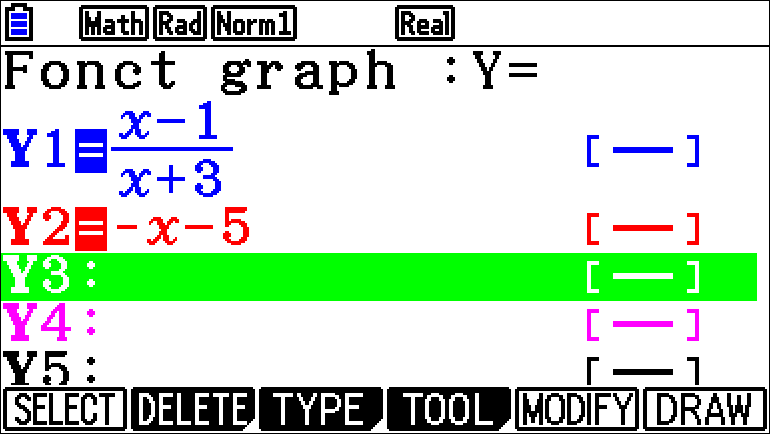
\includegraphics[height=3cm]{ch04_exos_corr_4a}~~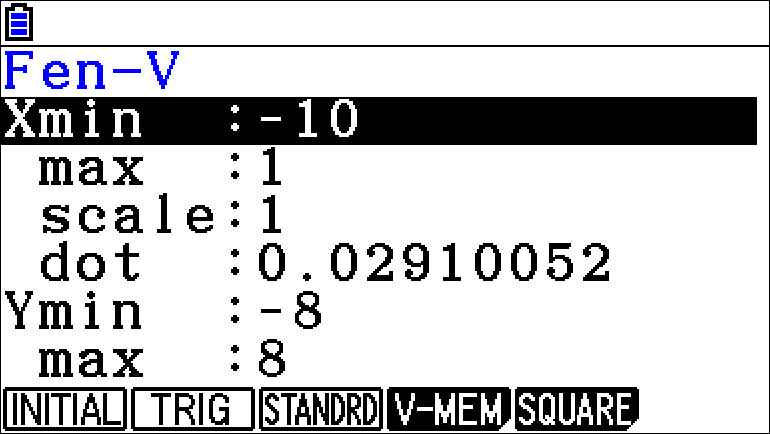
\includegraphics[height=3cm]{ch04_exos_corr_4b}~~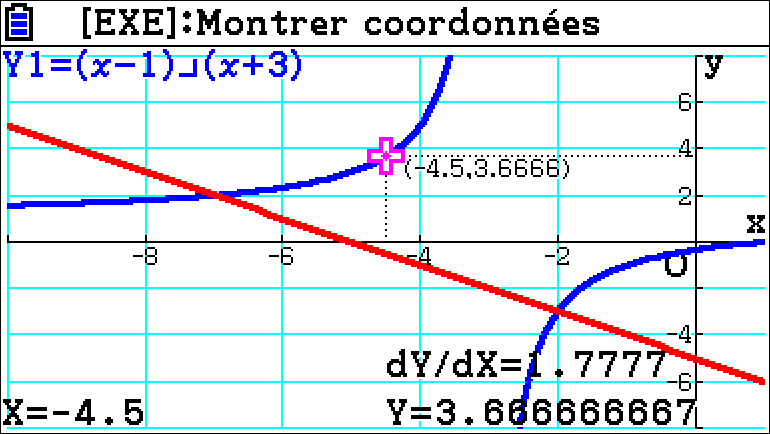
\includegraphics[height=3cm]{ch04_exos_corr_4c}
		\end{center}
		\item L'outil \ccalc{INTSECT} permet de déterminer les coordonnées des points d'intersection de $\mathcallig{C}_f$ et $\mathcallig{C}_g$ :
		
		\hfill{}$(-7\,;\,2)$ et $(-2\,;\,-3)$\hfill~
		
		\begin{center}
			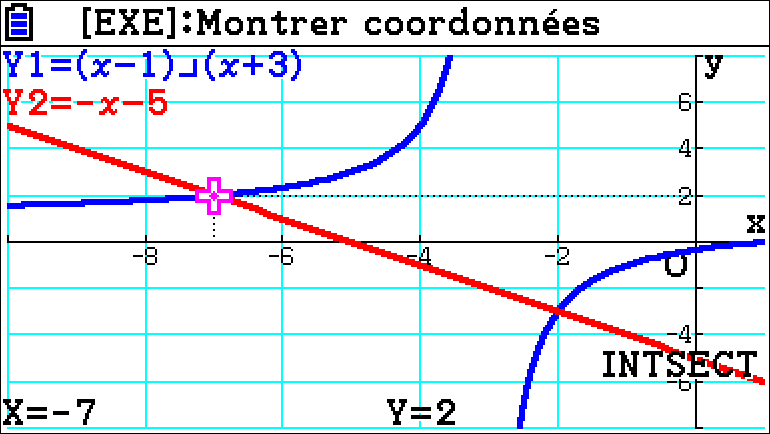
\includegraphics[height=3cm]{ch04_exos_corr_4d}~~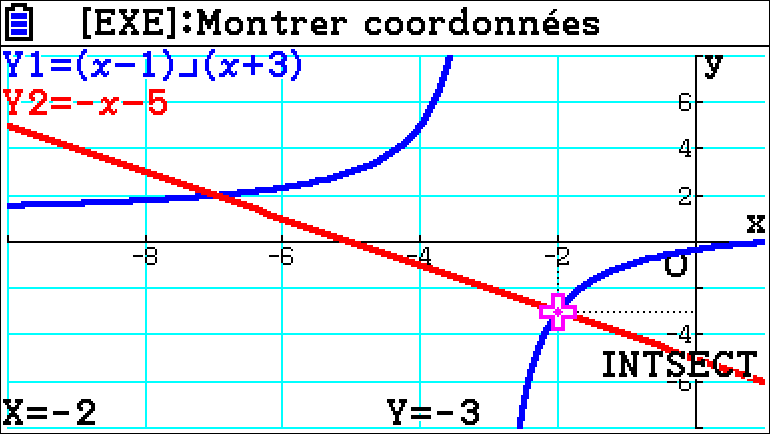
\includegraphics[height=3cm]{ch04_exos_corr_4e}
		\end{center}
		\item La calculatrice permet de conjecturer que :
		
		\tabula{} sur l'intervalle $\intervOO{-\infty}{-7}$, $\mathcolor{red}{\mathcallig{C}_f}$ est au-dessus de $\mathcolor{blue}{\mathcallig{C}_g}$ ;
		
		\tabula{} sur l'intervalle $\intervOO{-7}{-3}$, $\mathcolor{red}{\mathcallig{C}_f}$ est en-dessous de $\mathcolor{blue}{\mathcallig{C}_g}$ ;
		
		\tabula{} sur l'intervalle $\intervOO{-3}{-2}$, $\mathcolor{red}{\mathcallig{C}_f}$ est au-dessus de $\mathcolor{blue}{\mathcallig{C}_g}$ ;
		
		\tabula{} sur l'intervalle $\intervOO{-2}{+\infty}$, $\mathcolor{red}{\mathcallig{C}_f}$ est en-dessous de $\mathcolor{blue}{\mathcallig{C}_g}$ ;
		
		\tabula{}$\mathcolor{red}{\mathcallig{C}_f}$ et $\mathcolor{blue}{\mathcallig{C}_g}$ se croisent aux points de coordonnées $(-7\,;\,2)$ et $(-2\,;\,-3)$.
	\end{enumerate}
	\item On a $f(x)-g(x) = \dfrac{x-1}{x+3}-(-x-5) = \dfrac{x-1}{x+3}+x+5=\dfrac{x-1}{x+3}+\dfrac{(x+5)(x+3)}{x+3}= \dfrac{x-1+x^2+3x+5x+15}{x+3}$.
	
	Soit encore $f(x)-g(x) = \dfrac{x^2+9x+14}{x+3}$ qui est bien sous forme \textsf{Produit/Quotient} :
	
	\tabula{}$\bullet~~x^2+9x+14=0$ : $\Delta=25$, les racines sont $x_1=-2$ et $x_2=-7$ avec le signe $\oplus\ominus\oplus$ ;
	
	\tabula{}$\bullet~~x+3=0 \ssi x=-3$ et le signe est $\ominus\oplus$.
	
	\begin{center}
		\begin{tikzpicture}
			\tkzTabSetup[doubledistance=2pt]
			\tkzTabInit[lgt=4,espcl=2]{$x$/0.8,$x^2+9x+14$/0.8,$x+3$/0.8,$f(x)-g(x)$/0.8,$\text{pos. rel.}$/1.4}{$-\infty$,$-7$,$-3$,$-2$,$+\infty$}
			\draw(N31) node [yshift=1pt] {{\scriptsize \red \textsf{D}}};
			\draw (N24) --($(N25)+(-3pt,0)$) ; \draw (N24) --($(N25)+(3pt,0)$) ;
			\draw (N44) --($(N45)+(-3pt,0)$) ; \draw (N44) --($(N45)+(3pt,0)$) ;
			\draw (N25) node [below,font=\scriptsize] {$(-7\,;\,2)$};
			\draw (N45) node [below,font=\scriptsize] {$(-2\,;\,-3)$};
			\tkzTabLine{,+,z,-,t,-,z,+,}
			\tkzTabLine{,-,t,-,z,+,t,+,}
			\tkzTabLine{,-,z,+,d,-,z,+,}
			\tkzTabLine{,\mathscr{C}_g \text{ dessus},,\mathscr{C}_f \text{ dessus},d,\mathscr{C}_g \text{ dessus},,\mathscr{C}_f \text{ dessus},}
			\aidesignetkztabPL[code=pa+d+,racines={-7/-2},couleur=purple]{1}[0.75][1.5]
			\aidesignetkztabPL[code=da+,racines={-3},couleur=ForestGreen]{2}[0.75][1.5]
		\end{tikzpicture}
	\end{center}
\end{enumerate}



\end{document}

\clearpage

% !TeX TXS-program:compile = txs:///lualatex

\documentclass[a4paper,11pt]{article}
\usepackage[breakable]{cp-base}
\graphicspath{{./graphics/}}
%variables
\donnees[%
	typedoc=CHAPITRE~,
	numdoc=5,
	classe=1\up{ère} 2M2,
	matiere={[SPÉ.MATHS]},
	annee=2021,
	titre={Probas conditionnelles, indépendance}
	]

%formatage
\author{Pierquet}
\title{\nomfichier}
\hypersetup{pdfauthor={Pierquet},pdftitle={\nomfichier},allbordercolors=white,pdfborder=0 0 0,pdfstartview=FitH}
%divers
\lhead{\entete{\matiere}}
\chead{\entete{\lycee}}
\rhead{\entete{\classe{} - Chapitre \thepart}}
\lfoot{\pied{\matiere}}
\cfoot{\logolycee{}}
\rfoot{\pied{\numeropagetot}}
\usepackage{setspace}

\begin{document}

\pagestyle{fancy}

\part{CH05 - Probabilités conditionnelles, indépendance}

\section{Rappels sur les probabilités}

\subsection{Généralités}

\begin{cdefi}[s]
L'ensemble de toutes les \textbf{issues} (ou \textbf{éventualités}) possibles d'une expérience aléatoire s'appelle l'\textbf{univers} de cette expérience aléatoire (souvent noté $\Omega$).

Un sous-ensemble de cet univers s'appelle un \textbf{événement}.
\end{cdefi}

\begin{cprop}
Une probabilité est toujours un nombre compris \textbf{entre 0 et 1}.

Dans le cas où toutes les issues sont \textbf{équiprobables} (c'est-à-dire qu'elles ont toutes les mêmes chances de se produire), la \textbf{probabilité} d'un événement est le quotient : \[p(A)=\dfrac{\text{nombre de cas favorables à } A}{\text{nombre de cas possibles dans l'univers}}.\]
\end{cprop}

\begin{chistoire}
\vspace{-0.22cm}
\lettrine[findent=.5em,nindent=0pt,lines=3,image,novskip=0pt]{huygens}{}\uline{Huygens} ($1629-1695$, $\vcenter{\hbox{
\includegraphics[height=0.5\baselineskip]{nl}}}$) et Cardan ($1501-1576$, $\vcenter{\hbox{
\includegraphics[height=0.5\baselineskip]{it}}}$) sont considérés comme les \og pères de la théorie des probabilités \fg. Cependant la mauvaise réputation de Cardan a fait pencher la paternité sur Pascal et Fermat. L'apparition de la notion de « risque », préalable à l'étude des probabilités, n'est apparue qu'au XII\up{e} siècle pour l'évaluation de contrats commerciaux avec le \textit{Traité des contrats} de Pierre de Jean Olivia.

Les idées se propagent en Italie et en France, Galilée écrit entre 1620 en 1718 son petit mémoire sur le jeu de dés intitulé \textit{Sopra le Scoperte de i Dadi} dans lequel il suppose l'équipossibilité des lancers. Cette notion d'équipossibilité se retrouve également, plus tard, dans la correspondance de Pierre de Fermat et dans celle de Pierre-Simon de Laplace.
\end{chistoire}

\subsection{Événements, calculs de probabilités}

\begin{cdefi}[s]
L'événement \textbf{contraire} (ou complémentaire) $\overline{A}$ d'un événement $A$ se réalise dès que $A$ ne se réalise pas:

\begin{center}
	\begin{tikzpicture}[scale=0.6]
		\draw (-3,-1.5) rectangle (3,1.5) ;
		\draw  (0,0) circle (2cm and 1cm) ;
		\fill[pattern=north west lines]  (0,0) circle (2cm and 1cm);
		\draw (0,-1.5) node[below] {\vphantom{$\overline{A}$}$A$} ;
	\end{tikzpicture}
	\hspace{0.5cm}
	\begin{tikzpicture}[scale=0.6]
		\draw (-3,-1.5) rectangle (3,1.5) ;
		\fill[pattern=north west lines]  (-3,-1.5) rectangle (3,1.5) ;
		\draw  (0,0) circle (2cm and 1cm);
		\fill[ForestGreen!15]  (0,0) circle (2cm and 1cm);
		\draw (0,-1.5) node[below] {$\overline{A}$} ;
	\end{tikzpicture}
\end{center}
\vspace{-0.2cm}
L'\textbf{intersection $A \cap B$ } (lire \og $A$ inter $B$ \fg) de deux événements est l'événement qui se réalise lorsque $A$ \textbf{ET} $B$ se réalisent \emph{simultanément}.

La \textbf{réunion} $A \cup B$ (lire \og $A$ union $B$ \fg) de deux événements est l'événement qui se réalise lorsque l'\emph{un au moins} des deux événements se réalise (l'un \textbf{OU} l'autre \textbf{OU} les deux).

\begin{center}
	\begin{tikzpicture}[scale=0.8]
		\draw (-3,-2) rectangle (5,1.5) ;
		\draw (2,-0.5) circle (2cm and 1cm);
		\draw (0,0) circle (2cm and 1cm);
		\draw (1,-2) node[below] {$A \cap B$} ;
		\clip (2,-0.5) circle (2cm and 1cm);
		\fill[pattern=north west lines]  (0,0) circle (2cm and 1cm);
	\end{tikzpicture}
	\hspace{0.5cm}
	\begin{tikzpicture}[scale=0.8]
		\draw (-3,-2) rectangle (5,1.5) ;
		\draw (2,-0.5) circle (2cm and 1cm);
		\draw (0,0) circle (2cm and 1cm);
		\fill[pattern=north west lines]  (0,0) circle (2cm and 1cm);
		\fill[pattern=north west lines]  (2,-0.5) circle (2cm and 1cm);
		\draw (1,-2) node[below] {$A \cup B$} ;
	\end{tikzpicture}
\end{center}
\end{cdefi}

\begin{cprop}[s]
Quels que soient les événements $A$ et $B$ :
\begin{itemize}
	\item $p(\overline{A})=1-p(A)$ ;
	\item $p(A \cup B)=p(A)+p(B)-p(A \cap B)$.\hfill{\red\itshape formule de la réunion}
\end{itemize}
\end{cprop}

\begin{cexemple}[ : test pharmaceutique]
Un laboratoire pharmaceutique a réalisé des tests sur 800 patients atteints d’une maladie. Certains sont traités avec le médicament A, d’autres avec le médicament B.

Le tableau ci-dessous présente les résultats de l’étude :
\begin{center}
	\begin{tabularx}{14cm}{|Y|Y|Y|Y|}
	\cline{2-4}
	\multicolumn{1}{c|}{}& Médicament A & Médicament B & Total \\
	\hline
	Guéri & 383 & 291 & 674 \\
	\hline
	Non Guéri & 72 & 54 & 126 \\
	\hline
	Total & 455 & 345 & 800 \\
	\hline
\end{tabularx}
\end{center} 
On choisit au hasard un patient testé, et on appelle $A$ l'événement \og le patient a été traité avec le médicament A \fg{} et $G$ : \og il est guéri \fg.
\begin{itemize}[leftmargin=*]
	\item $\overline{A}$ est l'événement : \og le patient a été traité avec le médicament B \fg{} ;
	\item $A \cap G$ est l'événement : \og le patient a été traité avec le médicament A \textbf{et} est guéri \fg{} ;
	\item $A \cup G$ est l'événement : \og le patient a été traité avec le médicament A \textbf{ou} est guéri \fg.
\end{itemize}
On a, de plus :
\begin{itemize}[leftmargin=*]
	\item $p(\overline{A})=1-p(A)=1-\dfrac{455}{800}=\dfrac{345}{800}$ ;
	\item $p(A \cap G)=\dfrac{383}{800}$ ;
	\item $p(A \cup G)=p(A)+p(G)-p(A \cap G)=\dfrac{455}{800}+\dfrac{674}{800}-\dfrac{383}{800}=\dfrac{746}{800}$.
\end{itemize}
\end{cexemple}

\section{Arbre pondéré, probabilités conditionnelles}

\subsection{Utilisation d'un arbre pondéré}

\begin{cdefi}
Un \textbf{arbre pondéré} est un arbre de choix dans lequel les \textbf{branches} n'ont pas toutes le même poids. Chacune des branches (primaire ou secondaire) est alors affectée d'un nombre précisant la \textbf{probabilité} de passer par ce chemin plutôt qu'un autre.

À la \textbf{racine} de l'arbre, on trouve toujours l'univers de l'expérience aléatoire, et à chaque \textbf{noeud} ou \textbf{feuille}, un événement.
\end{cdefi}

\begin{cillustr}
\begin{center}
	% Racine à Gauche, développement vers la droite
	\begin{tikzpicture}[xscale=1,yscale=1]
		% Styles (MODIFIABLES)
		\tikzstyle{fleche}=[->,>=latex,thick]
		\tikzstyle{noeud}=[font=\sffamily\small]
		\tikzstyle{feuille}=[font=\sffamily\small,ForestGreen]
		\tikzstyle{etiquette}=[midway,fill=white,sloped,font=\sffamily\footnotesize]
		% Dimensions (MODIFIABLES)
		\def\DistanceInterNiveaux{5}
		\def\DistanceInterFeuilles{1.5}
		% Dimensions calculées (NON MODIFIABLES)
		\def\NiveauA{(0)*\DistanceInterNiveaux}
		\def\NiveauB{(1.25)*\DistanceInterNiveaux}
		\def\NiveauC{(2.5)*\DistanceInterNiveaux}
		\def\InterFeuilles{(-1)*\DistanceInterFeuilles}
		% Noeuds (MODIFIABLES : Styles et Coefficients d'InterFeuilles)
		\node[noeud] (R) at ({\NiveauA},{(1.5)*\InterFeuilles}) {\red racine};
		\node[noeud] (Ra) at ({\NiveauB},{(0.5)*\InterFeuilles}) {\blue nœud};
		\node[feuille] (Raa) at ({\NiveauC},{(0)*\InterFeuilles}) {feuille};
		\node[feuille] (Rab) at ({\NiveauC},{(1)*\InterFeuilles}) {feuille};
		\node[noeud] (Rb) at ({\NiveauB},{(2.5)*\InterFeuilles}) {\blue nœud};
		\node[feuille] (Rba) at ({\NiveauC},{(2)*\InterFeuilles}) {feuille};
		\node[feuille] (Rbb) at ({\NiveauC},{(3)*\InterFeuilles}) {feuille};
		% Arcs (MODIFIABLES : Styles)
		\draw[fleche] (R)--(Ra) node[etiquette] {branche primaire};
		\draw[fleche] (Ra)--(Raa) node[etiquette] {branche secondaire};
		\draw[fleche] (Ra)--(Rab) node[etiquette] {branche secondaire};
		\draw[fleche] (R)--(Rb) node[etiquette] {branche primaire};
		\draw[fleche] (Rb)--(Rba) node[etiquette] {branche secondaire};
		\draw[fleche] (Rb)--(Rbb) node[etiquette] {branche secondaire};
	\end{tikzpicture}
\end{center}
%:-+-+-+-+- Fin
\end{cillustr}

\begin{cexemple}[ : tirage dans une urne]
Un sac contient 20 boules rouges et 30 boules bleues. Chacune d'entre elles porte l'une des mentions \og Gagné \fg{} ou \og Perdu \fg. 15 boules rouges et 9 boules bleues sont gagnantes.

On tire au hasard une boule dans le sac, et on appelle $R$ l'événement \og La boule tirée est rouge \fg{} et $G$ \og La boule tirée est gagnante \fg. On peut schématiser cette expérience par l'arbre pondéré :	
	\begin{center}
		%urne
		\begin{tikzpicture}[scale=0.7]
			%urne
			\draw[rounded corners,ultra thick] (0,7) -- (0,0) -- (10,0) -- (10,7) ;
			\foreach \centre in {0.5,1.5,...,9.5}
			\filldraw[line width=1pt,black,fill=red] (\centre,0.5) circle(0.5) node{\bfseries\white\sf G} ;
			\foreach \centre in {0.5,1.5,...,4.5}
			\filldraw[line width=1pt,black,fill=red] (\centre,1.5) circle(0.5) node{\bfseries\white\sf G} ;
			\foreach \centre in {5.5,6.5,...,9.5}
			\filldraw[line width=1pt,black,fill=red] (\centre,1.5) circle(0.5) node{\bfseries\white\sf P} ;
			\foreach \centre in {0.5,1.5,...,8.5}
			\filldraw[line width=1pt,black,fill=blue] (\centre,2.5) circle(0.5) node{\bfseries\white\sf G} ;
			\filldraw[line width=1pt,black,fill=blue] (9.5,2.5) circle(0.5) node{\bfseries\white\sf P} ;
			\foreach \centre in {0.5,1.5,...,9.5}
			\filldraw[line width=1pt,black,fill=blue] (\centre,3.5) circle(0.5) node{\bfseries\white\sf P} ;
			\foreach \centre in {0.5,1.5,...,9.5}
			\filldraw[line width=1pt,black,fill=blue] (\centre,4.5) circle(0.5) node{\bfseries\white\sf P} ;
		\end{tikzpicture}
		\hspace{0.5cm}
		% Racine à Gauche, développement vers la droite
		\begin{tikzpicture}[xscale=1,yscale=1]
			% Styles (MODIFIABLES)
			\tikzstyle{fleche}=[->,>=latex,thick]
			\tikzstyle{noeud}=[font=\sffamily\small]
			\tikzstyle{feuille}=[font=\sffamily\small]
			\tikzstyle{etiquette}=[midway,fill=SeaGreen!5,font=\sffamily\footnotesize]
			% Dimensions (MODIFIABLES)
			\def\DistanceInterNiveaux{3}
			\def\DistanceInterFeuilles{1.5}
			% Dimensions calculées (NON MODIFIABLES)
			\def\NiveauA{(0)*\DistanceInterNiveaux}
			\def\NiveauB{(1.35)*\DistanceInterNiveaux}
			\def\NiveauC{(2.7)*\DistanceInterNiveaux}
			\def\InterFeuilles{(-1)*\DistanceInterFeuilles}
			% Noeuds (MODIFIABLES : Styles et Coefficients d'InterFeuilles)
			\node[noeud] (R) at ({\NiveauA},{(1.5)*\InterFeuilles}) {$\Omega$};
			\node[noeud] (Ra) at ({\NiveauB},{(0.5)*\InterFeuilles}) {$R$};
			\node[feuille] (Raa) at ({\NiveauC},{(0)*\InterFeuilles}) {$G$};
			\node[feuille] (Rab) at ({\NiveauC},{(1)*\InterFeuilles}) {$\overline{G}$};
			\node[noeud] (Rb) at ({\NiveauB},{(2.5)*\InterFeuilles}) {$\overline{R}$};
			\node[feuille] (Rba) at ({\NiveauC},{(2)*\InterFeuilles}) {$G$};
			\node[feuille] (Rbb) at ({\NiveauC},{(3)*\InterFeuilles}) {$\overline{G}$};
			% Arcs (MODIFIABLES : Styles)
			\draw[fleche] (R)--(Ra) node[etiquette] {$\frac{20}{50}=0,4$};
			\draw[fleche] (Ra)--(Raa) node[etiquette] {$\frac{15}{20}=0,75$};
			\draw[fleche] (Ra)--(Rab) node[etiquette] {$\frac{5}{20}=0,25$};
			\draw[fleche] (R)--(Rb) node[etiquette] {$\frac{30}{50}=0,6$};
			\draw[fleche] (Rb)--(Rba) node[etiquette] {$\frac{9}{30}=0,3$};
			\draw[fleche] (Rb)--(Rbb) node[etiquette] {$\frac{21}{30}=0,7$};
		\end{tikzpicture}
	\end{center}
\end{cexemple}

\begin{cexercice}[ : test pharmaceutique]
Décrire la situation à l'aide d'un arbre pondéré.
\end{cexercice}

\begin{cthm}[s]
\vspace{-0.2cm}
\begin{itemize}[leftmargin=*]
	\item La somme des probabilités de toutes les branches partant d'un même noeud est toujours égale à 1.
	\item La probabilité d'un chemin est égale au produit des probabilités de toutes les branches qui le composent.
	\item La probabilité d'un événement est la somme des probabilités de tous les chemins qui mènent à cet événement.
\end{itemize}
\end{cthm}

\begin{cexemple}[ : tirage dans une urne]
La probabilité d'obtenir une boule rouge gagnante est $\tfrac{15}{50}=\tfrac{3}{10}=p(R \cap G)$.

\tabula{}Sur l'arbre, on retrouve bien  $0,4 \times 0,75 = 0,3$.

La probabilité d'obtenir une boule gagnante est $\tfrac{15+9}{50}=0,48$.

Sur l'arbre,  il y a deux chemins qui mènent à $G$ : le chemin $R \cap G$, de probabilité $0,3$ et le chemin $\overline{R} \cap G$ de probabilité $0,6 \times 0,3=0,18$. On retrouve bien $p(R \cap G)+p(\overline{R} \cap G)=0,3+0,18= 0,48=p(G)$.
\end{cexemple}

\begin{cexercice}[ : test pharmaceutique]
En utilisant l'arbre pondéré ci-dessus, déterminer $p(A)$, $p(B \cap G)$, $p(G)$, $p(\overline{G})$.
\end{cexercice}

\subsection{Probabilité conditionnelle}

\begin{cdefi}
Lorsqu'on construit un arbre pondéré comme ci-dessus, les probabilités inscrites sur les branches primaires sont des probabilités classiques, mais les probabilités inscrites sur les branches secondaires sont des \textbf{probabilités conditionnelles} : ce sont les probabilités d'arriver à ce nœud \emph{sachant que l'on vient de tel autre nœud}.

La probabilité conditionnelle que l'événement $B$ se réalise sachant que l'événement $A$ est réalisé  se note $p_A(B)$ (lire \og probabilité de $B$ sachant $A$ \fg) et, si $p(A) \neq 0$ :\[p_A(B)=\dfrac{p(A \cap B)}{p(A)}.\]
\end{cdefi}

\begin{crmq}[s]
\vspace{-0.2cm}
\begin{itemize}[leftmargin=*]
	\item Si $p(B) \neq 0$, on peut inverser les rôles de $A$ et $B$ dans la formule ci-dessus : $ p_B(A)=\dfrac{p(A \cap B)}{p(B)}$.
	\item Si les probabilités conditionnelles du type $p_A(B)$ sont en général données dans les énoncés, il arrive souvent qu'on doive inverser les conditions et calculer par exemple $p_B(A)$. C'est là que la formule est nécessaire.
\end{itemize}
\end{crmq}

\begin{cexemple}
$p_{R}(G)=0,75$ est la probabilité de tirer une boule gagnante \textit{sachant qu'elle est rouge}, autrement dit, la probabilité de tirer une boule rouge gagnante \textit{parmi les rouges}. Cette probabilité découle de la constitution de l'urne.

\smallskip

$p_{G}(R)$ ne figure pas dans l'arbre. C'est la probabilité d'avoir tiré une boule rouge \textit{sachant qu'elle est marquée gagnante}, autrement dit la probabilité de tirer une boule rouge gagnante \textit{parmi les boules gagnantes}. C'est moins naturel dans ce sens, puisqu'on voit la couleur de la boule avant d'y trouver la marque.

\hfill$p_{G}(R)=\frac{p(G \cap R)}{p(G)}=\frac{0,3}{0,48}=0,625$.\hfill~

On peut tout de même retrouver cette probabilité grâce à la constitution de l'urne : sur les $15+9=24$ boules gagnantes, il y en a 15 rouges et $\frac{15}{24}=0,625$.
\end{cexemple}

\begin{cexercice}[ : test pharmaceutique]
Calculer $p_G(A)$ de deux façons différentes : en utilisant l'arbre puis en utilisant le tableau à double entrée.
\end{cexercice}

\begin{cprop}[s]
$\bullet~~p(A \cap B)=p(A) \times p_A(B)$.\hfill{\red\itshape formule des probabilités composées}

$\bullet~~p_A(\overline{B})=1-p_A(B)$.
\end{cprop}

\begin{cdemoblanc}
\vspace{-0.2cm}
\begin{itemize}[leftmargin=*]
	\item C'est la formule que l'on utilise quand on dit que la probabilité d'un chemin est le produit de celles des branches qui le composent : \[p_A(B)=\dfrac{p(A \cap B)}{p(A)} \ssi p(A \cap B)=p(A) \times p_A(B).\]
	\item C'est la formule que l'on utilise quand on dit que la somme des probabilités des branches issues d'un même nœud est toujours égale à 1 : \vspace{-0.2cm}
	\begin{center}
		\begin{tikzpicture}[scale=0.5]
			\draw (2,-0.5) circle (2cm and 1cm);
			\draw (0,0) circle (2cm and 1cm);
			\draw (1,-1.5) node[below] {$A \cap B$} ;
			\clip (2,-0.5) circle (2cm and 1cm);
			\fill[pattern=north west lines]  (0,0) circle (2cm and 1cm);
		\end{tikzpicture}
		\hspace{0.5cm}
		\begin{tikzpicture}[scale=0.5]
			\fill[pattern=north west lines]  (0,0) circle (2cm and 1cm);
			\draw (2,-0.5) circle (2cm and 1cm);
			\fill[white]  (2,-0.5) circle (2cm and 1cm);
			\draw (0,0) circle (2cm and 1cm);
			\draw (1,-1.5) node[below] {$A \cap \overline{B}$} ;
		\end{tikzpicture}
	\end{center} \vspace{-0.2cm}
	En effet, la réunion de $A \cap B$ et $A \cap \overline{B}$ est égale à $A$ donc $p_A(\overline{B})+p_A(B)=\frac{p(A \cap \overline{B})}{p(A)}+\frac{p(A \cap B)}{p(A)}=\frac{p(A)}{p(A)}=1$.
\end{itemize}
\end{cdemoblanc}

\subsection{Formule des probabilités totales}

\begin{cdefi}[ : Partition de l'univers]
Soient $A_1, A_2, ..., A_n$ une liste d'évènements relatifs à une même expérience aléatoire.\\ On dit que ces événements réalisent une \textbf{partition} de l'univers si :
\begin{itemize}
	\item aucun de ces éléments n'est vide ;
	\item ils sont deux à deux disjoints (c'est-à-dire d'intersection vide) ;
	\item la réunion de tous ces événements recouvre l'univers tout entier.
\end{itemize}
\end{cdefi}

\begin{crmq}
En particulier, un événement $A$ et son événement contraire $\overline{A}$ forment une partition de $\Omega$.
\end{crmq}

\begin{cillustr}
Pour une partition à 4 éléments :
\begin{center}
	\begin{tikzpicture}[scale=0.65]
		\draw[rounded corners=6pt,ultra thick] (0,0) rectangle (7,3) ;
		%abscisses ligne du bas = 0 / 2 / 3.5 / 4.5 / 7 
		\draw[ultra thick] (1,3) -- (2,0) ;
		\draw[ultra thick] (3,3) -- (3.5,0) ;
		\draw[ultra thick] (4.5,0) -- (7,2.5) ;
		\tikzset{texte/.style={above,font=\blue\bfseries\small}}
		\draw (1,0) node[texte] {$\mathsf{A_1}$} ;
		\draw (2.75,0) node[texte] {$\mathsf{A_2}$} ;
		\draw (4,0) node[texte] {$\mathsf{A_3}$} ;
		\draw (5.75,0) node[texte] {$\mathsf{A_4}$} ;
	\end{tikzpicture}
\end{center}
\end{cillustr}

\begin{cthm}[ : Formule des probabilités totales]
Si les événements $A_1, A_2, ..., A_n$ réalisent une partition de l'univers, alors pour tout événement $B$ : \[p(B)=p(A_1 \cap B)+p(A_2 \cap B)+...+p(A_n \cap B).\]%
En particulier, pour tous événements $A$ et $B$ : \[p(B)=p(A \cap B) + p(\overline{A} \cap B).\]
\end{cthm}

\begin{cdemoblanc}[]
C'est la propriété qu'on utilise quand on dit que la probabilité d'un événement est la somme de toutes les probabilités des chemins qui mènent à cet événement. Elle vient du fait que les événements $A_1~\cap~B$, $A_2~\cap~B$,\ldots, $A_n~\cap~B$ sont deux à deux disjoints et recouvrent entièrement $B$.
\begin{center}
	\begin{tikzpicture}[scale=0.65]
		\draw[rounded corners=6pt,ultra thick] (0,0) rectangle (7,3) ;
		\draw[ultra thick] (1,3) -- (2,0) ;
		\draw[ultra thick] (3,3) -- (3.5,0) ;
		\draw[ultra thick] (4.5,0) -- (7,2.5) ;
		\tikzset{texte/.style={above,font=\blue\bfseries\small}}
		\draw (1,0) node[texte] {$\mathsf{A_1}$} ;
		\draw (2.75,0) node[texte] {$\mathsf{A_2}$} ;
		\draw (4,0) node[texte] {$\mathsf{A_3}$} ;
		\draw (5.75,0) node[texte] {$\mathsf{A_4}$} ;
		%ellipse
		\draw[ultra thick,rotate around={-10:(3.5,1.5)},red,fill=red!33,fill opacity=0.33] (3.5,1.65) ellipse (3 and 0.75);
	\end{tikzpicture}
\end{center}
\end{cdemoblanc}

\begin{cillustr}
Sur un arbre, on peut visualiser et représenter différentes probabilités mises en jeu :
\begin{itemize}
	\item des \textcolor{purple}{conditionnelles} ;
	\item les \textcolor{ForestGreen}{composées} ;
	\item les \textcolor{red}{totales}.
\end{itemize}
\begin{center}
	\begin{tikzpicture}[xscale=1,yscale=1]
		% Styles (MODIFIABLES)
		\tikzstyle{fleche}=[->,>=latex,thick]
		\tikzstyle{noeud}=[font=\small]
		\tikzstyle{feuille}=[ForestGreen,font=\small]
		\tikzstyle{etiquette}=[midway,sloped,font=\small]
		\tikzstyle{notice}=[font=\sffamily\small]
		% Dimensions (MODIFIABLES)
		\def\DistanceInterNiveaux{3}
		\def\DistanceInterFeuilles{1.5}
		% Dimensions calculées (NON MODIFIABLES)
		\def\NiveauA{(0)*\DistanceInterNiveaux}
		\def\NiveauB{(1.35)*\DistanceInterNiveaux}
		\def\NiveauC{(2.7)*\DistanceInterNiveaux}
		\def\NiveauD{(3.5)*\DistanceInterNiveaux}
		\def\NiveauE{(5)*\DistanceInterNiveaux}
		\def\InterFeuilles{(-1)*\DistanceInterFeuilles}
		% Noeuds (MODIFIABLES : Styles et Coefficients d'InterFeuilles)
		\node[noeud] (R) at ({\NiveauA},{(1.5)*\InterFeuilles}) {$\Omega$};
		\node[noeud] (Ra) at ({\NiveauB},{(0.5)*\InterFeuilles}) {$A$};
		\node[noeud] (Raa) at ({\NiveauC},{(0)*\InterFeuilles}) {$B$};
		\node[noeud] (Rab) at ({\NiveauC},{(1)*\InterFeuilles}) {$\overline{B}$};
		\node[noeud] (Rb) at ({\NiveauB},{(2.5)*\InterFeuilles}) {$\overline{A}$};
		\node[noeud] (Rba) at ({\NiveauC},{(2)*\InterFeuilles}) {$B$};
		\node[noeud] (Rbb) at ({\NiveauC},{(3)*\InterFeuilles}) {$\overline{B}$};
		% Arcs (MODIFIABLES : Styles)
		\draw[fleche,above] (R)--(Ra) node[etiquette,blue] {$p(A)$};
		\draw[fleche,above] (Ra)--(Raa) node[etiquette,purple] {$p_{A}(B)$};
		\draw[fleche,below] (Ra)--(Rab) node[etiquette,purple] {$p_{A}(\overline{B})=1-p_{A}(B)$};
		\draw[fleche,below] (R)--(Rb) node[etiquette,blue] {$p(\overline{A})$};
		\draw[fleche,above] (Rb)--(Rba) node[etiquette,purple] {$p_{\overline{A}}(B)$};
		\draw[fleche,below] (Rb)--(Rbb) node[etiquette,purple] {$p_{\overline{A}}(\overline{B})=1-p_{\overline{A}}(B)$};
		%feuilles
		\node[feuille] (F1) at ({\NiveauD},{(0)*\InterFeuilles}) {$p\left(A \cap B \right) = p(A) \times p_A(B)$};
		\node[feuille] (F2) at ({\NiveauD},{(1)*\InterFeuilles}) {$p\left(A \cap \overline{B} \right) = p(A) \times p_{\overline{A}}(B)$};
		\node[feuille] (F3) at ({\NiveauD},{(2)*\InterFeuilles}) {$p\left(\overline{A} \cap B \right) = p(\overline{A}) \times p_{\overline{A}}(B)$};
		\node[feuille] (F4) at ({\NiveauD},{(3)*\InterFeuilles}) {$p\left({\overline{A}} \cap \overline{B} \right) = p(\overline{A}) \times p_{\overline{A}}({\overline{B}})$};
		%totales
		\node[feuille,red,inner sep=1pt] (T1) at ({\NiveauE},{(0.5)*\InterFeuilles}) {$p(B)=p\left(A \cap B \right) +p\left(\overline{A} \cap B \right)$};
		\node[feuille,red,inner sep=1pt] (T2) at ({\NiveauE},{(2.5)*\InterFeuilles}) {$p(\overline{B})=p\left(A \cap \overline{B} \right) +p\left(\overline{A} \cap \overline{B} \right)$};
		%fléches dashed
		\draw[fleche,densely dashed,red] (F1.east) to [out=-15,in=135] (T1.north) ;
		\draw[fleche,densely dashed,red] (F3.east) to [out=15,in=-135] (T1.south) ;
		\draw[fleche,densely dashed,red] (F2.east) to [out=-15,in=135] (T2.north) ;
		\draw[fleche,densely dashed,red] (F4.east) to [out=15,in=-135] (T2.south) ;
		%notices
		\draw[notice,purple] ({(0.5)*\NiveauB+(0.5)*\NiveauC},{(-0.5)*\InterFeuilles}) node {probabilités conditionnelles} ;
		\draw[notice,ForestGreen] ({\NiveauD},{(-0.5)*\InterFeuilles}) node {probabilités composées} ;
		\draw[notice,red] ({\NiveauE},{(-0.5)*\InterFeuilles}) node {probabilités totales} ;
	\end{tikzpicture}
\end{center}
\end{cillustr}

\newpage

\section{Indépendance}

\subsection{Événements indépendants}

\begin{cdefi}[ - Propriété]
On dit que deux événements  de probabilités non nulles sont \textbf{indépendants} s'ils vérifient l'une ou l'autre des propriétés ci-dessous, qui sont équivalentes : \[ p(A \cap B)=p(A) \times p(B) \ssi p_A(B)=p(B) \ssi p_B(A)=p(A).\]%
Autrement dit, la réalisation d'un événement n'influence pas la probabilité de l'autre.
\end{cdefi}

\begin{cdemoblanc}
En effet, a priori on a $p(A \cap B)=p(A) \times p_A(B) $ donc si les événements sont indépendants :

\tabula{}$p(A \cap B)=p(A) \times p(B) = p(A) \times p_A(B) $ et donc si $p(A) \neq 0$, on retrouve bien $ p(B) =  p_A(B) $. 
\end{cdemoblanc}

\begin{cexemple}
On tire une carte au hasard dans un jeu de 32 cartes. On appelle $C$ l'événement \og Obtenir un cœur \fg{} et $D$ \og Obtenir une dame \fg. $C \cap D$ est alors \og Obtenir la dame de cœur \fg.

\begin{center}
	\def\hauteur{1}
	\poker{7C}{\hauteur}~\poker{8C}{\hauteur}~\poker{9C}{\hauteur}~\poker{10C}{\hauteur}~\poker{VC}{\hauteur}~\poker{DC}{\hauteur}~\poker{RC}{\hauteur}~\poker{AC}{\hauteur}~\poker{DK}{\hauteur}~\poker{DP}{\hauteur}~\poker{DT}{\hauteur}
\end{center}

\smallskip

$\bullet~~p(C)=\frac{8}{32}=\frac{1}{4}$ et $p(D)=\frac{4}{32}=\frac{1}{8}$ et
$p(C \cap D)=\frac{1}{32}$ et $\frac{1}{4} \times \frac{1}{8} = \frac{1}{32}$ donc $C$ et $D$ sont indépendants. 

\smallskip

On a aussi $p_C(D)=p(D)$, c'est-à-dire que la probabilité d'obtenir une dame parmi les cœurs est la même que celle d'obtenir une dame parmi toutes les cartes : $\frac{1}{8}$ .

\medskip

Maintenant, si on rajoute deux jokers dans le jeu :

\smallskip

$\bullet~~p(C)=\frac{8}{34}$ et $p(D)=\frac{4}{34}$ et
$p(C \cap D)=\frac{1}{34}$ et $p(C) \times p(D) = \frac{8 \times 4}{34 \times 34} \neq p(C \cap D)$ donc $C$ et $D$ pas indépendants. 

\smallskip

De même, $p_C(D)=\frac{1}{8}$ mais $p(D)= \frac{4}{34}$ et ces probabilités ne sont plus égales.
\end{cexemple}

\begin{cprop}
Si $A$ et $B$ sont indépendants, alors $\overline{A}$ et $B$ sont indépendants.
\end{cprop}

\begin{cdemoblanc}
$p(\overline{A} \cap B)+p(A \cap B)=p(B)$ d'après la formule des probabilités totales, donc, si $A$ et $B$ sont indépendants, \\ $p(\overline{A} \cap B)+p(A) \times p(B) = p(B)$ et ainsi $p(\overline{A} \cap B)=p(B)-p(A) \times p(B) = p(B)(1-p(A))=p(B)\times p(\overline{A})$.
\end{cdemoblanc}

\subsection{Expériences indépendantes}

\begin{cdefi}
Lorsque deux expériences aléatoires se succèdent et que les résultats de la première n'ont aucune influence sur les résultats de la seconde, on dit qu'il s'agit d'une \textbf{succession d'épreuves indépendantes}.
\end{cdefi}

\begin{cexemple}
On tire au hasard successivement deux cartes dans un jeu de 32 cartes.

Si on remet la carte avant le deuxième tirage, les conditions initiales sont identiques, donc on peut considérer que les deux tirages sont indépendants.

Si on ne remet pas la carte, la constitution du paquet dépend de la première carte tirée, donc les expériences ne sont pas indépendantes.
\end{cexemple}


\begin{cprop}[ (admise)]
Lorsque deux épreuves sont indépendantes, la probabilité d'un couple de résultats est égale au produit des probabilités de chacun d'eux.
\end{cprop}

\begin{cexemple}
On lance deux fois de suite un dé cubique.

La probabilité d'obtenir un double 5 est $\frac{1}{6} \times \frac{1}{6}$.
\end{cexemple}

\vfill{}

\begin{chistoire}[ - Anecdote]
\begin{minipage}{0.33\linewidth}
	\begin{center}
		\includegraphics[width=4cm]{chap05_table}
	\end{center}
\end{minipage}\hfill
\begin{minipage}{0.65\linewidth}
\begin{center}
	\includegraphics[height=1.25cm]{chap05_pascalfermat}
\end{center}
\setstretch{0.7}{\policeqtcanaithtype\scriptsize Le \textit{chevalier de Méré} (17\up{e} siècle) était un joueur et souhaitait connaître les stratégies amenant à un plus grand nombre de succès. Il soumet ce problème : « Deux joueurs misent chacun 32 pistoles dans un jeu en trois manches gagnantes. La partie est interrompue alors que le premier joueur a remporté deux manches et le second une seule. Quel doit être alors le gain de chacun des deux joueurs ? » Pascal et Fermat relèvent le défi et on retrouve les réponses dans leurs échanges épistolaires.
 Le problème décrit par le chevalier de Méré est un problème historique que l’on trouve déjà dans le \textit{Summa de Arithmetica} de Luca Pacioli (1494). Pascal et Fermat sont les premiers à y apporter une solution mathématique généralisable.\\ C’est cependant le Hollandais Christiaan Huygens qui publie en 1657 le premier traité mathématique consacré aux probabilités : \textit{Tractatus de Rariociniis in Alea Ludo}. De nos jours, les probabilités constituent une partie très importante des mathématiques.}
\end{minipage}

~\hfill{}{\tiny Source : \textit{LeLivreScolaire}}
\end{chistoire}

\begin{chumour}
	\vspace{-0.2cm}
	\begin{center}
		\includegraphics[width=8cm]{chap05_devin}
		
		{\tiny Source : \textit{Astérix}, Uderzo \& Goscinny}
	\end{center}
\end{chumour}

\end{document}

\clearpage

\setcounter{numexos}{0}

% !TeX TXS-program:compile = txs:///lualatex

\documentclass[a4paper,11pt]{article}
\usepackage[revgoku]{cp-base}
\graphicspath{{./graphics/}}
%variables
\donnees[
	classe={1\up{ère} 2M2},matiere={[SPÉ.MATHS]},mois=Janvier,annee=2022,typedoc=CHAP,numdoc=5
]
%formatage
\author{Pierquet}
\title{\nomfichier}
\hypersetup{pdfauthor={Pierquet},pdftitle={\nomfichier},allbordercolors=white,pdfborder=0 0 0,pdfstartview=FitH}
\lhead{\entete{\matiere}}
\chead{\entete{\lycee}}
\rhead{\entete{\classe{} - \mois{} \annee}}
\lfoot{\pied{\matiere}}
\cfoot{\logolycee{}}
\rfoot{\pied{\numeropagetot}}
%divers

\begin{document}

\pagestyle{fancy}

\part{CH05 - Probabilités conditionnelles, indépendance - Exercices}

\smallskip

\exonum{}

\medskip

En vue de sa prochaine brochure d'information sur les dangers des Réseaux Sociaux, un lycée a fait remplir un questionnaire à chacun des \num{2000}~élèves, répartis dans les sections de seconde, première et terminale. On obtient la répartition : 

\begin{itemize}
	\item un quart des élèves est en terminale ; 
	\item 35\,\% des élèves sont en première ; 
	\item tous les autres sont en seconde ; 
	\item parmi les élèves de terminale, 70\,\% utilisent régulièrement les Réseaux Sociaux ; 
	\item 630 élèves sont des élèves de première qui utilisent régulièrement les Réseaux Sociaux.
	\item \num{1740}~élèves utilisent régulièrement les Réseaux Sociaux.
\end{itemize}

Cette enquête permet de modéliser le choix d'un élève du lycée. On choisit au hasard un questionnaire d'élève en supposant que ce choix se fait en situation d'équiprobabilité. On note :

\begin{itemize}
	\item $S$ l'évènement \og le questionnaire est celui d'un élève en classe de seconde \fg ;
	\item $E$ l'évènement \og le questionnaire est celui d'un élève en classe de première \fg ;
	\item $T$ l'évènement \og le questionnaire est celui d'un élève en classe de terminale \fg ;
	\item $R$ l'évènement \og le questionnaire est celui d'un élève qui utilise régulièrement les Réseaux Sociaux (RS) \fg.
\end{itemize}

\begin{enumerate}
	\item Compléter le tableau d'effectifs ci-dessous.
	
	\smallskip
	
	\begin{tblr}{%
			width=\linewidth,colspec={l*{4}{X[c]}},
			vline{1}={2-Z}{solid},vline{2-Z}={solid},hline{1}={2-Z}{solid},hline{2-Z}={solid},
			rows={font=\sffamily}
		}
		& Seconde & Première & Terminale & Total\\
		Utilise régulièrement les RS 		&	&630&	&		\\
		N'utilise pas régulièrement les RS 	&	&	&	&		\\
		Total 								&	&	&	&2\,000	\\
	\end{tblr}
	\item Déterminer la probabilité d'obtenir le questionnaire d'un élève de seconde qui utilise régulièrement les RS. 
	\item Calculer la probabilité de $R$ sachant $T$, notée $p_{T}(R)$, et interpréter ce résultat à l'aide d'une phrase. 
	\item Calculer la probabilité que le questionnaire choisi soit celui d'un élève qui n'utilise pas les RS. 
	\item Le questionnaire est celui d'un élève qui utilise régulièrement les RS.
	
	Montrer que la probabilité que ce soit le questionnaire d'un élève de première est égale à $\frac{21}{58}$.
\end{enumerate}

\medskip

\exonum{}

\medskip

Une entreprise financière est divisée en deux secteurs ; 65\,\% de son personnel travaille dans le secteur A et 35\,\% dans le secteur B. Cette entreprise s'intéresse au niveau de stress de son personnel.
 
Une enquête, menée sous la forme d'un questionnaire informatisé, est réalisée au sein de l'entreprise. Le questionnaire est proposé de manière anonyme aux salariés des deux secteurs. Cette enquête révèle que pour le secteur A, 20\,\% du personnel se dit stressé, tandis que, dans le secteur B, ce taux est de 30\,\%. 

On choisit au hasard le questionnaire d'un employé de l'entreprise, chacun ayant la même probabilité d'être choisi. On note : 

\begin{itemize}
	\item A : \og le questionnaire est celui d'un employé du secteur A \fg. 
	\item B : \og le questionnaire est celui d'un employé du secteur B \fg. 
	\item S : \og le questionnaire est celui d'un employé stressé \fg.
\end{itemize}
 
\begin{enumerate}
	\item Construire un arbre pondéré décrivant la situation. 
	\item Calculer la probabilité que le questionnaire choisi soit celui d'un employé qui travaille dans le secteur B et qui est stressé. 
	\item L'entreprise examine l'opportunité d'installer une salle de relaxation. Si le taux d'employés stressés est strictement supérieur à 25\,\%, cette salle sera installée.
	 
	L'entreprise implantera-t-elle la salle de relaxation ? Justifier la réponse. 
	\item Sachant que le questionnaire choisi est celui d'un employé stressé, quelle est la probabilité qu'il travaille dans le secteur A ? (le résultat sera arrondi à $10^{-2}$)
\end{enumerate} 

\medskip

\exonum{}

\medskip

Un restaurant propose à sa carte deux types de dessert :

\begin{itemize}
	\item[$\bullet~$] un assortiment de macarons, choisi par 50\,\% des clients; 
	\item[$\bullet~$] une part de tarte tatin, choisie par 30\,\% des clients.
\end{itemize}
 
20\,\% des clients ne prennent pas de dessert et aucun client ne prend plusieurs desserts. Le restaurateur constate :

\begin{itemize}
	\item que parmi les clients ayant pris un assortiment de macarons, 80\,\% prennent un café ; 
	\item que parmi les clients ayant pris une part de tarte tatin, 60\,\% prennent un café; 
	\item que parmi les clients n'ayant pas pris de dessert, 90\,\% prennent un café.
\end{itemize}

On interroge au hasard un client de ce restaurant. On note $p$ la probabilité associée à cette expérience aléatoire. On note :

\begin{itemize}
	\item $M$ l'évènement : \og Le client prend un assortiment de macarons \fg{} ; 
	\item $T$ l'évènement : \og Le client prend une part de tarte tatin \fg{} ; 
	\item $P$ l'évènement : \og Le client ne prend pas de dessert \fg{} ; 
	\item $C$ l'évènement: \og Le client prend un café \fg{} et $\overline{C}$ l'évènement contraire de $C$.
\end{itemize}
 
\begin{enumerate}
	\item En utilisant les données de l'énoncé, préciser la valeur de $p(T)$ et celle de $p_{T}(C)$, probabilité de l'évènement $C$ sachant que $T$ est réalisé. 
	\item Recopier et compléter l'arbre ci-dessous: 
	
	\begin{center}
		\begin{tikzpicture}[scale=0.66]
		\tikzstyle{fleche}=[->,>=latex,thick]
		\tikzstyle{noeud}=[]
		\tikzstyle{feuille}=[]
		\tikzstyle{etiquette}=[pos=0.55,sloped,fill=white]
		
		\def\DistanceInterNiveaux{3}
		\def\DistanceInterFeuilles{1}
		
		\def\NiveauA{(0)*\DistanceInterNiveaux}
		\def\NiveauB{(1.5)*\DistanceInterNiveaux}
		\def\NiveauC{(3)*\DistanceInterNiveaux}
		\def\InterFeuilles{(-0.8)*\DistanceInterFeuilles}
		
		\node[noeud] (R) at ({\NiveauA},{(4)*\InterFeuilles}) {$ $};
		\node[noeud] (Ra) at ({\NiveauB},{(1)*\InterFeuilles}) {$M$};
		\node[feuille] (Raa) at ({\NiveauC},{(0)*\InterFeuilles}) {$C$};
		%\node[feuille] (Rab) at ({\NiveauC},{(1)*\InterFeuilles}) {$C_{n+1}$};
		\node[feuille] (Rac) at ({\NiveauC},{(2)*\InterFeuilles}) {$\overline{C}$};
		\node[noeud] (Rb) at ({\NiveauB},{(4)*\InterFeuilles}) {$T$};
		\node[feuille] (Rba) at ({\NiveauC},{(3)*\InterFeuilles}) {$C$};
		%\node[feuille] (Rbb) at ({\NiveauC},{(4)*\InterFeuilles}) {$B_{n+1}$};
		\node[feuille] (Rbc) at ({\NiveauC},{(5)*\InterFeuilles}) {$\overline{C}$};
		\node[noeud] (Rc) at ({\NiveauB},{(7)*\InterFeuilles}) {$P$};
		\node[feuille] (Rca) at ({\NiveauC},{(6)*\InterFeuilles}) {$C$};
		%\node[feuille] (Rcb) at ({\NiveauC},{(7)*\InterFeuilles}) {$A_{n+1}$};
		\node[feuille] (Rcc) at ({\NiveauC},{(8)*\InterFeuilles}) {$\overline{C}$};
		
		\draw[fleche] (R)--(Ra) node[etiquette] {$\num{0,5}$};
		\draw[fleche] (Ra)--(Raa) node[etiquette] {$\num{0,8}$};
		\draw[fleche] (Ra)--(Rac) node[etiquette] {$\ldots$};
		\draw[fleche] (R)--(Rb) node[etiquette] {$\ldots$};
		\draw[fleche] (Rb)--(Rba) node[etiquette] {$\ldots$};
		\draw[fleche] (Rb)--(Rbc) node[etiquette] {$\ldots$};
		\draw[fleche] (R)--(Rc) node[etiquette] {$\ldots$};
		\draw[fleche] (Rc)--(Rca) node[etiquette] {$\ldots$};
		\draw[fleche] (Rc)--(Rcc) node[etiquette] {$\ldots$};
		\end{tikzpicture}
	\end{center}
	\item  
		\begin{enumerate}
			\item Exprimer par une phrase ce que représente l'évènement $M \cap C$ puis calculer $p(M \cap C)$.
			\item Montrer que $p(C) = \num{0,76}$.
		\end{enumerate} 
	\item Quelle est la probabilité que le client prenne un assortiment de macarons sachant qu'il prend un café ?
	\item Un assortiment de macarons est vendu 6\,€, une part de tarte tatin est vendue 7\,€, et un café est vendu 2\,€.
	 
	Chaque client prend un seul plat au prix unique de 18\,€, ne prend pas plus d'un dessert ni plus d'un café.
 
	\begin{enumerate}
		\item Quelles sont les six valeurs possibles pour la somme totale dépensée par un client? 
		\item Reproduire et compléter le tableau ci-dessous donnant la loi de probas de la somme totale dépensée :
		
		\smallskip
		
		\begin{tabularx}{\linewidth}{|l|*{6}{>{\centering \arraybackslash}X|}}\hline
			Sommes $s_{i}$& 18 &20 &24 &\ldots&\ldots&\ldots\\ \hline
			$p\left(s_{i}\right)$&0,02&0,18&\ldots&&&\\ \hline 
		\end{tabularx}
	
		\smallskip
	\item Calculer l'espérance mathématique de cette loi et interpréter ce résultat. 
	\end{enumerate}
\end{enumerate}
%
%\medskip
%
%\exonum{}
%
%\medskip
%
%Une salle de jeu comporte deux consoles identiques proposant le même jeu. Un jour l'une des deux est déréglée.
%
%Les joueurs ne peuvent pas savoir laquelle des deux est déréglée. 
%
%\begin{enumerate}
%	\item Ce jour-là, un joueur choisit au hasard l'une des deux consoles et il joue une partie sur cette console.
%	
%	On note :
%	\begin{itemize}[topsep=1pt]
%		\item $D$ l'évènement \og le joueur choisit la console déréglée\fg{} et $\overline{D}$ l'évènement contraire ; 
%		\item $G$ l'évènement \og le joueur gagne la partie \fg{} et $\overline{G}$  l'évènement contraire. 
%	\end{itemize}
%	
%	Cette situation aléatoire est modélisée par l'arbre incomplet suivant, dans lequel figure certaines probas. 
%	
%	\begin{center}
%		\begin{tikzpicture}[xscale=0.9,yscale=0.9]
%			\tikzstyle{fleche}=[->,>=latex,thick]
%			\tikzstyle{noeud}=[]
%			\tikzstyle{feuille}=[]
%			\tikzstyle{etiquette}=[pos=0.55,sloped,fill=white]
%			
%			\def\DistanceInterNiveaux{3}
%			\def\DistanceInterFeuilles{0.85}
%			
%			\def\NiveauA{(0)*\DistanceInterNiveaux}
%			\def\NiveauB{(1.25)*\DistanceInterNiveaux}
%			\def\NiveauC{(2.5)*\DistanceInterNiveaux}
%			\def\InterFeuilles{(-1)*\DistanceInterFeuilles}
%			
%			\node[noeud] (R) at ({\NiveauA},{(1.5)*\InterFeuilles}) {$\Omega$};
%			\node[noeud] (Ra) at ({\NiveauB},{(0.5)*\InterFeuilles}) {$D$};
%			\node[feuille] (Raa) at ({\NiveauC},{(0)*\InterFeuilles}) {$G$};
%			\node[feuille] (Rab) at ({\NiveauC},{(1)*\InterFeuilles}) {$\overline{G}$};
%			\node[noeud] (Rb) at ({\NiveauB},{(2.5)*\InterFeuilles}) {$\overline{D}$};
%			\node[feuille] (Rba) at ({\NiveauC},{(2)*\InterFeuilles}) {$G$};
%			\node[feuille] (Rbb) at ({\NiveauC},{(3)*\InterFeuilles}) {$\overline{G}$};
%			
%			\draw[fleche] (R)--(Ra) node[etiquette] {${0,5}$};
%			\draw[fleche] (Ra)--(Raa) node[etiquette] {${0,7}$};
%			\draw[fleche] (Ra)--(Rab) node[etiquette] {$\ldots$};
%			\draw[fleche] (R)--(Rb) node[etiquette] {$ \ldots$};
%			\draw[fleche] (Rb)--(Rba) node[etiquette] {${0,2}$};
%			\draw[fleche] (Rb)--(Rbb) node[etiquette] {$\ldots$};
%		\end{tikzpicture}
%	\end{center}
%	
%	\begin{enumerate}
%		\item Compléter l'arbre de probabilité. 
%		\item Calculer la probabilité de l'évènement \og  le joueur choisit la console déréglée et il gagne \fg.
%		\item Calculer la probabilité de l'évènement \og le joueur choisit la console non déréglée et il gagne \fg.
%		\item Montrer que la probabilité que le joueur gagne est égale à $0,45$.
%		\item Calculer la probabilité que le joueur ait choisit la console déréglée sachant qu'il a gagné.
%	\end{enumerate}
%	\item Les évènements D et G sont-ils indépendants ? Justifier la réponse.
%	\item Calculer la probabilité de l'événement \og le joueur gagne trois parties de suite \fg{}.
%\end{enumerate}
%
%\medskip
%
%\exonum{}
%
%\medskip
%
%Un nouveau bachelier souhaitant souscrire un prêt automobile pour l'achat de sa première voiture, a le choix entre les trois agences bancaires de sa ville : agence A, agence B et agence C. Après vérification, on a constaté que :
%%
%\begin{itemize}
%	\item 20\:\% des prêts sont souscrits dans l'agence A,
%	\item 45\:\% des prêts sont souscrits dans l'agence B,
%	\item les autres prêts étant souscrits dans l'agence C. 
%\end{itemize}
%%  
%On suppose que tous les clients souscrivent à une assurance dans l'agence où le prêt est souscrit.
%
%Deux types de contrats sont proposés : le contrat tout risque, dit \emph{Zen} et le deuxième contrat appelé \emph{Speed}. 
%
%\medskip
%
%\hspace{5mm}-- 80\,\% des clients de l'agence A ayant souscrit un prêt automobile, souscrivent une assurance \emph{Zen}.
%
%\hspace{5mm}-- 30\,\% des clients de l'agence B ayant souscrit un prêt automobile, souscrivent une assurance \emph{Zen}. 
%
%\hspace{5mm}-- $\nicefrac{2}{7}$ des clients de l'agence C ayant souscrit un prêt automobile, souscrivent une assurance \emph{Speed}.
%
%\smallskip 
%
%On interroge au hasard un client d'une de ces trois banques ayant souscrit un contrat d'assurance automobile. 
%
%On considère les évènements suivants :
%
%\begin{itemize}
%	\item A : \og le prêt a été souscrit dans l'agence A \fg{},
%	\item B : \og le prêt a été souscrit dans l'agence B \fg{},
%	\item C : \og le prêt a été souscrit dans l'agence C \fg{}, 
%	\item Z : \og le contrat d'assurance \emph{Zen} a été souscrit \fg{}, 
%	\item S : \og le contrat d'assurance \emph{Speed} a été souscrit \fg{}.
%\end{itemize}
%
%\begin{enumerate}
%	\item Représenter la situation à l'aide d'un arbre pondéré. 
%	\item Déterminer la probabilité que le client interrogé ait souscrit un prêt automobile avec une assurance \emph{Zen} dans l'agence A. 
%	\item Vérifier que la probabilité de l'évènement Z est égale à $0,545$. 
%	\item Le client a souscrit une assurance \emph{Zen}. Déterminer la probabilité que le prêt soit souscrit dans l'agence C. 
%\end{enumerate}
%
%\medskip
%
%\exonum{}
%
%\medskip
%
%Un concessionnaire automobile vend deux versions de voitures pour une marque donnée: routière ou break. Pour chaque version il existe deux motorisations : essence ou diesel. Le concessionnaire choisit au hasard un client ayant déjà acheté une voiture. On note : 
%
%\begin{itemize}
%	\item $R$ l'évènement: \og la voiture achetée est une routière \fg{} ;
%	\item $B$ l'évènement: \og la voiture achetée est une break \fg{}; 
%	\item $E$ l'évènement : \og la voiture est achetée avec une motorisation essence \fg{} ;
%	\item $D$ l'évènement : \og la voiture est achetée avec une motorisation diesel \fg. 
%\end{itemize}
%%
%On sait que :
%%
%\begin{itemize}[topsep=1pt]
%	\item[$\bullet~$] 65\:\% des clients achètent une voiture routière. 
%	\item[$\bullet~$] Lorsqu'un client achète une voiture break, il choisit dans 85\:\% des cas la motorisation diesel. 
%	\item[$\bullet~$] $27,3$\:\% des clients achètent une voiture routière avec une motorisation diesel.
%\end{itemize}
%
%\begin{enumerate}
%	\item Quelle est la probabilité $p(R)$ de l'événement $R$ ? 
%	\item 
%	\begin{enumerate}
%		\item Construire l'arbre de probabilité (il sera complété ultérieurement). 
%		\item Démontrer que $P_{R}(D) = 0,42$ (probabilité de $D$ sachant $R$). 
%	\end{enumerate}
%	\item Calculer $p(D)$. 
%	\item Lorsque le concessionnaire a choisi au hasard un client, on note $X$ le prix de vente (en milliers d'euros) de la voiture achetée. Compléter le tableau suivant donnant la loi de probabilité de $X$.
%	
%	\renewcommand{\arraystretch}{1.3}
%	\begin{tabularx}{\linewidth}{|l|*{4}{Y|}}
%		\hline
%		Version &\multicolumn{2}{c}{Routière} &\multicolumn{2}{c}{Break} \\ \hline
%		Motorisation &Essence&Diesel &Essence &Diesel \\ \hline
%		$x_{i}$ : prix de vente (en milliers d'€) &15 &18 &17 &20\\ \hline 
%		$P_{i}$ : probabilité&& $0,273$&&\\ \hline
%	\end{tabularx} 
%	
%	Calculer l'espérance mathématique de $X$. Quelle interprétation peut-on en donner ? 
%\end{enumerate}
%
%\medskip
%
%\exonum{}
%
%\medskip
%
%Une boîte de chocolats contient 50\,\% de chocolats au lait, 30\,\% de chocolats noirs et 20\,\% de chocolats blancs. Tous les chocolats de la boîte sont de même forme et d'emballage identique. 
%
%Ils sont garnis soit de praliné soit de caramel et, parmi les chocolats au lait, 56\,\% sont garnis de praliné.
%
%On choisit au hasard un chocolat de la boîte. On suppose que tous les choix sont équiprobables. On note :
%%
%\begin{itemize}
%	\item[$\bullet~$] L : l'évènement \og le chocolat choisi est au lait \fg{} ; 
%	\item[$\bullet~$] N : l'évènement \og le chocolat choisi est noir \fg{} ; 
%	\item[$\bullet~$] B : l'évènement \og le chocolat choisi est blanc \fg{} ; 
%	\item[$\bullet~$] P : l'évènement \og le chocolat choisi est garni de praliné \fg{} ; 
%	\item[$\bullet~$] C : l'évènement \og le chocolat choisi est garni de caramel \fg. 
%\end{itemize}
%
%
%\begin{enumerate}
%	\item Traduire les données du problème à l'aide d'un arbre de probabilité. 
%	\item  Donner la probabilité que le chocolat choisi soit garni de praliné sachant que c'est un chocolat au lait. 
%	\item Déterminer la probabilité  que le chocolat choisi soit au lait et garni de praliné. 
%	\item Dans la boîte, 21\,\% des chocolats sont noirs et garnis de praliné. 
%	
%	Montrer que la probabilité que le chocolat choisi soit garni de praliné, sachant que c'est un chocolat noir, est égale à $0,7$. 
%	\item Dans la boîte, 60\,\% des chocolats sont garnis de praliné. 
%	\begin{enumerate}
%		\item Déterminer la probabilité que le chocolat choisi soit blanc et garni de praliné. 
%		
%		\item En déduire la probabilité que le chocolat choisi soit garni de praliné sachant que c'est un chocolat blanc. 
%	\end{enumerate}
%	\item On dispose de deux boîtes de chocolats identiques à celle décrite précédemment. Une personne prend au hasard un chocolat dans la première boîte, puis un chocolat dans la deuxième boîte (les tirages sont indépendants). 
%	
%	Déterminer la probabilité de l'évènement : \og l'un des chocolats choisi est garni de praliné et l'autre est garni de caramel \fg.
%\end{enumerate}
%
%\medskip
%
%\exonum{}
%
%\medskip
%
%Un site Internet offre la possibilité à des particuliers de vendre des objets aux enchères. Pour chaque objet, la durée des enchères dure une semaine. Si une annonce reçoit une enchère, alors la vente de l'objet est obligatoire à la fin des enchères et ce, même si le vendeur juge le prix de vente trop peu élevé.
%
%Sur ce site une étude statistique a montré que :
%
%\begin{itemize}
%	\item[$\bullet$] $\nicefrac{3}{5}$ des annonces reçoivent une première enchère le lendemain de leur parution ; dans  ce cas, 75\,\% des vendeurs sont satisfaits du prix de vente final ;
%	\item[$\bullet$] $\nicefrac{1}{3}$ des annonces reçoit une première enchère au bout de trois jours et, dans ce cas, 57\,\% des vendeurs sont satisfaits du prix de vente final de leur objet ;
%	\item[$\bullet$] les autres annonces ne reçoivent aucune enchère et le vendeur retire alors son objet de la vente. 
%\end{itemize}
%%
%On choisit au hasard une annonce mise en ligne sur le site. On note :
%%
%\begin{itemize}
%	\item[$\bullet$] L : l'évènement \og l'annonce reçoit une première enchère le lendemain de sa parution \fg ; 
%	\item[$\bullet$] T : l'évènement \og  l'annonce reçoit une première enchère au bout de trois jours \fg ; 
%	\item[$\bullet$] A: l'évènement \og l'annonce ne reçoit aucune enchère \fg ; 
%	\item[$\bullet$] S : l'évènement \og le vendeur est satisfait du prix de vente final de son objet \fg ~et $\overline{S}$ son évènement contraire. 
%\end{itemize}
%
%\begin{enumerate}
%	\item Traduire la situation par un arbre de probabilités. 
%	\item Calculer la probabilité que l'annonce ait reçu une première enchère le lendemain de sa parution et que le vendeur soit satisfait du prix de vente final. 
%	\item Démontrer que la probabilité que le vendeur soit satisfait du prix de vente de son objet est $0,64$. 
%	\item Un objet est vendu à un prix qui satisfait son vendeur. Quelle est la probabilité que cet objet ait reçu une première enchère dès le lendemain de la parution de l'annonce (le résultat sera donné sous forme décimale, arrondi au centième) ? 
%	\item Marc a mis en vente le même jour trois jeux vidéo identiques sur ce site. On suppose que les déroulements des enchères sont indépendants les uns des autres.
%	
%	Calculer la probabilité qu'à la fin des enchères, Marc soit satisfait du prix de vente de tous ses jeux vidéo (arrondie au centième). 
%\end{enumerate}
%
%\medskip
%
%\begin{center}
%	\includegraphics[scale=0.20]{chap05_exov2_humour} 
%	
%	{\scriptsize \textit{Le Devin}, Uderzo \& Goscinny}
%\end{center}

\end{document}

\clearpage

\setcounter{numexos}{0}

% !TeX TXS-program:compile = txs:///arara
% arara: lualatex: {shell: no, synctex: yes, interaction: batchmode}
% arara: pythontex: {rerun: modified} if exists('pytxcode') && found('pytxcode', 'PYTHONTEX#py')
% arara: lualatex: {shell: no, synctex: yes, interaction: batchmode} if exists('pytxcode') && found('pytxcode', 'PYTHONTEX#py')
% arara: lualatex: {shell: no, synctex: yes, interaction: batchmode} if found('log', '(undefined references|Please rerun|Rerun to get)')

\documentclass[a4paper,11pt]{article}
\usepackage[revgoku]{cp-base}
\graphicspath{{./graphics/}}
%variables
\donnees[
	classe={1\up{ère} 2M2},matiere={[SPÉ.MATHS]},mois=Janvier,annee=2022,typedoc=CHAP,numdoc=5,tailletitre=\LARGE
]
%formatage
\author{Pierquet}
\title{\nomfichier}
\hypersetup{pdfauthor={Pierquet},pdftitle={\nomfichier},allbordercolors=white,pdfborder=0 0 0,pdfstartview=FitH}
\lhead{\entete{\matiere}}
\chead{\entete{\lycee}}
\rhead{\entete{\classe{} - \mois{} \annee}}
\lfoot{\pied{\matiere}}
\cfoot{\logolycee{}}
\rfoot{\pied{\numeropagetot}}
%divers

\begin{document}

\pagestyle{fancy}

\part{CH05 - Probabilités conditionnelles, indépendance - Exercices (Correction)}

\smallskip

\exonum{}

\begin{enumerate}
	\item Compléter le tableau d'effectifs ci-dessous.
	
	\smallskip
	
	\begin{tblr}{%
			width=\linewidth,colspec={l*{4}{X[c]}},
			vline{1}={2-Z}{solid},vline{2-Z}={solid},hline{1}={2-Z}{solid},hline{2-Z}={solid},
			rows={font=\sffamily}
		}
		& Seconde & Première & Terminale & Total\\
		Utilise régulièrement les RS 		&760	&630		&350		&\np{1740} \\
		N'utilise pas régulièrement les RS 	&40		&70			&150		&260 \\
		Total 								&800	&700		&500		&\np{2000} \\
	\end{tblr}
	
	$\blacktriangleright$~~Élèves de terminale : $\dfrac{1}{4} \times \np{2000} = 500$.
	
	$\blacktriangleright$~~Élèves de première : $\dfrac{35}{100} \times \np{2000} = 700$ ; il reste donc  $\np{2000} - (500 + 700) = 800$ élèves en seconde.
	
	$\blacktriangleright$~~Nombre d'élèves de terminale utilisant internet : $\dfrac{70}{100} \times500 = 350$.
	
	$\blacktriangleright$~~Nombre d'élèves de seconde utilisant internet : par différence : $\np{1740} - (350 + 630) = 760$.
	\item La probabilité d'obtenir le questionnaire d'un élève de 2\up{de} qui utilise régulièrement les RS est $\dfrac{760}{\np{2000}} = 0,38$.
	\item On a $P(T) = \dfrac{1}{4} = 0,25$ et  $P_{T}(R) = \dfrac{P(T \cap R)}{P(T)} = \dfrac{\frac{350}{2000}}{\frac{1}{4}} = \dfrac{350}{500} = 0,7$. C'est la probabilité qu'un élève de terminale rencontré au hasard utilise les RS, et cette donnée est dans l'énoncé !
	\item  Sur \np{2000} élèves 260 n'utilisent pas les RS régulièrement. $P\left(\overline{R}\right) = \dfrac{260}{2000} = \dfrac{13}{100} = 0,13$.
	\item Sur les \np{1740} utilisateurs réguliers il y a 630 élèves de première ; la probabilité est donc $P_R(E) = \dfrac{630}{\np{1740}} = \dfrac{21}{58}$.
\end{enumerate}

\medskip

\exonum{}

\begin{enumerate}
	\item On peut proposer l'arbre suivant :
	
	\begin{center}
		\begin{tikzpicture}[xscale=1,yscale=1]
			\tikzstyle{fleche}=[->,>=latex,thick]
			\tikzstyle{noeud}=[]
			\tikzstyle{feuille}=[]
			\tikzstyle{etiquette}=[pos=0.55,sloped,fill=white]
			
			\def\DistanceInterNiveaux{3}
			\def\DistanceInterFeuilles{1}
			
			\def\NiveauA{(0)*\DistanceInterNiveaux}
			\def\NiveauB{(1.25)*\DistanceInterNiveaux}
			\def\NiveauC{(2.5)*\DistanceInterNiveaux}
			\def\InterFeuilles{(-1)*\DistanceInterFeuilles}
			
			\node[noeud] (R) at ({\NiveauA},{(1.5)*\InterFeuilles}) {$\Omega$};
			\node[noeud] (Ra) at ({\NiveauB},{(0.5)*\InterFeuilles}) {$A$};
			\node[feuille] (Raa) at ({\NiveauC},{(0)*\InterFeuilles}) {$S$};
			\node[feuille] (Rab) at ({\NiveauC},{(1)*\InterFeuilles}) {$\overline{S}$};
			\node[noeud] (Rb) at ({\NiveauB},{(2.5)*\InterFeuilles}) {$B$};
			\node[feuille] (Rba) at ({\NiveauC},{(2)*\InterFeuilles}) {$S$};
			\node[feuille] (Rbb) at ({\NiveauC},{(3)*\InterFeuilles}) {$\overline{S}$};
			
			\draw[fleche] (R)--(Ra) node[etiquette] {${0,65}$};
			\draw[fleche] (Ra)--(Raa) node[etiquette] {${0,2}$};
			\draw[fleche] (Ra)--(Rab) node[etiquette] {${0,8}$};
			\draw[fleche] (R)--(Rb) node[etiquette] {${0,35}$};
			\draw[fleche] (Rb)--(Rba) node[etiquette] {${0,3}$};
			\draw[fleche] (Rb)--(Rbb) node[etiquette] {${0,7}$};
		\end{tikzpicture}
	\end{center}
	\item La probabilité que le questionnaire choisi soit celui d'un employé qui travaille dans le secteur B et qui est stressé est $p(B \cap S)$.
	
	D'après la formule des probabilités composées, $p(B \cap S) = p(B) \times p_{B}(S) = 0,35 \times 0,3 = 0,105$. 
	\item D'après la formule des probabilités totales : $p(S) =  p(A \cap S) + p(B \cap S) = 0,13 + 0,105 = 0,235$.
	
	Le résultat obtenu correspond à 23,5\,\% : la salle de relaxation ne sera pas installée.
	\item Il faut trouver $p_{S}(A) = \dfrac{p(S \cap A)}{p(A)} = \dfrac{0,13}{0,235} \approx 0,55$ au centième près.
\end{enumerate} 

\pagebreak

\exonum{}

\begin{enumerate}
	\item L'énoncé nous donne $p(T) = 0,3$ et  $P_{T}(C)  = 0,6$.
	\item L'arbre de probabilités est : 
	
	\begin{center}
		\begin{tikzpicture}[scale=0.66]
			\tikzstyle{fleche}=[->,>=latex,thick]
			\tikzstyle{noeud}=[]
			\tikzstyle{feuille}=[]
			\tikzstyle{etiquette}=[pos=0.55,sloped,fill=white,scale=0.9]
			\tikzstyle{vide}=[]
			\def\DistanceInterNiveaux{3}
			\def\DistanceInterFeuilles{1}
			\def\NiveauA{(0)*\DistanceInterNiveaux}
			\def\NiveauB{(1.5)*\DistanceInterNiveaux}
			\def\NiveauC{(3)*\DistanceInterNiveaux}
			\def\InterFeuilles{(-1)*\DistanceInterFeuilles}
			\node[noeud] (R) at ({\NiveauA},{(4)*\InterFeuilles}) {$\Omega$};
			\node[noeud] (Ra) at ({\NiveauB},{(1)*\InterFeuilles}) {$M$};
			\node[feuille] (Raa) at ({\NiveauC},{(0)*\InterFeuilles}) {$C$};
			\node[feuille] (Rac) at ({\NiveauC},{(2)*\InterFeuilles}) {$\overline{C}$};
			\node[noeud] (Rb) at ({\NiveauB},{(4)*\InterFeuilles}) {$T$};
			\node[feuille] (Rba) at ({\NiveauC},{(3)*\InterFeuilles}) {$C$};
			\node[feuille] (Rbc) at ({\NiveauC},{(5)*\InterFeuilles}) {$\overline{C}$};
			\node[noeud] (Rc) at ({\NiveauB},{(7)*\InterFeuilles}) {$P$};
			\node[feuille] (Rca) at ({\NiveauC},{(6)*\InterFeuilles}) {$C$};
			\node[feuille] (Rcc) at ({\NiveauC},{(8)*\InterFeuilles}) {$\overline{C}$};
			\draw[fleche] (R)--(Ra) node[etiquette] {$0,5$};
			\draw[fleche] (Ra)--(Raa) node[etiquette] {$0,8$};
			\draw[fleche] (Ra)--(Rac) node[etiquette] {$0,2$};
			\draw[fleche] (R)--(Rb) node[etiquette] {$0,3$};
			\draw[fleche] (Rb)--(Rba) node[etiquette] {$0,6$};
			\draw[fleche] (Rb)--(Rbc) node[etiquette] {$0,4$};
			\draw[fleche] (R)--(Rc) node[etiquette] {$0,2$};
			\draw[fleche] (Rc)--(Rca) node[etiquette] {$0,9$};
			\draw[fleche] (Rc)--(Rcc) node[etiquette] {$0,1$};
		\end{tikzpicture}
	\end{center}
	\item 
	\begin{enumerate}
		\item $M \cap C$ représente l'évènement \og le client a pris un macaron \textbf{et} un café \fg.
		
		Et on a $p(M \cap C) = p(M) \times p_M(C) = 0,5 \times 0,8 = 0,4$. 
		\item D'après la formule des probabilités totales, on a $p(C) = p(M \cap C) + p(T \cap C) + p(P \cap C)$.
		
		Et donc $p(C) = 0,4 + 0,3 \times 0,6 + 0,2 \times 0,9 =  0,4 + 0,18 + 0,18 = 0,76$.
	\end{enumerate} 
	\item Il faut trouver $p_C (M) = \dfrac{p(C \cap M)}{p(C)} = \dfrac{0,4}{0,76} \approx 0,53$ à 0,01 près.
	\item
	\begin{enumerate}
		\item On a :
		
		\tabula{}$\bullet~~P + M + C$ : 18 + 6 + 2 = 26~\euro ;
		
		\tabula{}$\bullet~~P + M$ : 18 + 6 = 24~\euro ;
		
		\tabula{}$\bullet~~P + T + C$ : 18 + 7 + 2 = 27~\euro ;
		
		\tabula{}$\bullet~~P + T$ : 18 + 7 = 25~\euro ;
		
		\tabula{}$\bullet~~P + C$  : 18 + 2 = 20~\euro ;
		
		\tabula{}$\bullet~~P$ : 18~\euro
		\item le tableau complété est :
		
		\smallskip
		
		\begin{tabularx}{\linewidth}{|l|*{6}{>{\centering \arraybackslash}X|}}\hline
			Sommes $s_{i}$& 18 &20 &24 &\ldots&\ldots&\ldots\\ \hline
			$p\left(s_{i}\right)$&$0,02$&$0,18$	&$0,1$	&$0,12$	&$0,4$	&$0,18$\\ \hline 
		\end{tabularx}
		
		\smallskip
		\item On a $18 \times 0,02 + 20 \times0,18 + 24 \times0,1 + 25 \times0,12 + 26 \times 0,4 + 27 \times 0,18 = 24,62$~(\euro).
		
		Sur un grand nombre de repas la recette par client s'élève à 24,62~\euro. 
	\end{enumerate}
\end{enumerate}

\end{document}

\clearpage

% !TeX TXS-program:compile = txs:///lualatex

\documentclass[a4paper,11pt]{article}
\usepackage[breakable]{cp-base}
\graphicspath{{./graphics/}}
%variables
\donnees[%
	typedoc=CHAPITRE~,numdoc=6,classe=1\up{ère} 2M2,matiere={[SPÉ.MATHS]}
]

%formatage
\author{Pierquet}
\title{\nomfichier}
\hypersetup{pdfauthor={Pierquet},pdftitle={\nomfichier},allbordercolors=white,pdfborder=0 0 0,pdfstartview=FitH}
%divers
\lhead{\entete{\matiere}}
\chead{\entete{\lycee}}
\rhead{\entete{\classe{} - Chapitre \thepart}}
\lfoot{\pied{\matiere}}
\cfoot{\logolycee{}}
\rfoot{\pied{\numeropagetot}}
\usepackage{setspace}

\begin{document}

\pagestyle{fancy}

\part{CH06 - Trigonométrie}

\section{Mesure d'angle en radians}

\subsection{Le cercle trigonométrique}

\begin{cdefi}
Dans un repère orthonormé $\Rij$, le \textbf{cercle trigonométrique} est le cercle \emph{orienté} de centre $O$, de rayon 1 et parcouru dans le \emph{sens inverse des aiguilles d'une montre}.
\end{cdefi}

\begin{cillustr}
\vspace{-0.2cm}
\begin{center}
	\tikzset{cross/.style={%
			cross out,draw=black,minimum size=2*(#1-\pgflinewidth),inner sep=0pt,outer sep=0pt},%
			cross/.default={1pt}}
	\begin{tikzpicture}[x=1.25cm,y=1.25cm,line width=1.25pt]
		\draw[->,>=stealth] (-1.15,0) -- (3,0) ; \draw[->,>=stealth] (0,-1.15) -- (0,1.75) ;
		\draw[blue] (0,0) circle[radius=1] ;
		\draw[blue] (135:1.2) node {\footnotesize \sf (C)};
		\draw[line width=1pt] (1,0) node[cross=3pt,black]{};
		\draw (0,1) node[above left=0pt] {\footnotesize \sf J} (1,0) node[above right=0pt] {\footnotesize \sf 1} (1,0) node[below right=0pt] {\footnotesize \sf I} ;
		\draw (2,0) node[above] {\tiny \sf axe des abscisses} ;
		\draw[ForestGreen,->,>=stealth] (25:1.5) arc (25:65:1.5) ;
		\draw[ForestGreen] (45:1.65) node {\small \sf +};
	\end{tikzpicture}
\end{center}
\end{cillustr}

\begin{crmq}
Le sens de parcours sur le cercle trigonométrique s'appelle le sens \emph{direct}, le sens \emph{trigonométrique} ou encore sens \emph{positif}.
\end{crmq}

\subsection{Longueur d'arc et mesure en radian}

\begin{cprop}
Si $I$ est le point de coordonnées $(1\,;\,0)$ et $M$ est un point du cercle trigonométrique, alors la longueur de l'arc $\overparen{IM}$ (exprimée dans l'unité de longueur du repère) est proportionnelle à la mesure de l'angle $\widehat{IOM}$.
\end{cprop}

\begin{cdefi}
La \textbf{mesure en radians} d'un angle est égale à la \textbf{longueur de l'arc} qu'il intercepte sur le cercle trigonométrique.
\end{cdefi}

\begin{cillustr}
\vspace{-0.2cm}
\begin{center}
	\tunits{1.25}{1.25}
	\tdefgrille{-1.15}{3}{1}{1}{-1.15}{1.5}{1}{1}
	\begin{tikzpicture}[x=\xunit cm,y=\yunit cm,line width=1.25pt]
		\draw[ForestGreen,fill=ForestGreen!50,opacity=0.5] (0,0) -- (0.48,0) arc (0:130:0.48) -- cycle ;
		\axestikz*[typefleche=stealth] ;
		\axextikz[size=\footnotesize]{-1,1,2} ;
		\axeytikz[size=\footnotesize]{-1,1} ;
		\draw (0,0) node[below left] {\footnotesize $0$} ;
		\draw[darkgray] (0,0) node[above right] {\small \sf O} (1,0) node[above right] {\small \sf I} (130:1) node[above] {\small \sf M} ;
		\draw[blue] (0,0) circle[radius=1] ; \draw (0,0) -- (130:1) ;
		\draw[red,line width=1.5pt] (1,0) arc (0:130:1) ;
		\foreach \Point in {(0,0),(1,0),(130:1)} \draw[line width=0.75pt,darkgray,fill=gray] \Point circle[radius=2pt] ;
		\draw[ForestGreen] (0.20,0.6) node {\tiny \sf Angle de $\mathsf{\theta}$ radians};
		\draw[red] (65:1.05) node[right] {\tiny \sf Arc de $\mathsf{\theta}$ unités de longueur};
	\end{tikzpicture}
\end{center}
\end{cillustr}

\begin{crmq}[ - Exemple]
Les mesures en radians ou en degrés sont donc proportionnelles. Un angle de $\pi$ radians mesure 180\ensuremath{^\circ} donc une simple règle de proportionnalité permet de convertir d'une unité à l'autre : {\footnotesize \begin{tabularx}{1.5cm}{Y|Y} 180&$\pi$ \\ \hline $d$&$r$ \end{tabularx}}.

Par exemple, $90\ensuremath{^\circ} = \dfrac{\pi}{2}$ rad  ; $\frac{2\pi}{3} \text{rad} =  120 \ensuremath{^\circ}$.
\end{crmq}

\section{Enroulement autour du cercle}

\subsection{Le principe}

\begin{cdefi}
Dans un repère orthonormé $\Rij$, on considère le cercle trigonométrique $\mathscr{C}$ ; le point $I$ de coordonnées $(1\,;\,0)$ et  la tangente $\mathscr{D}$ à $\mathscr{C}$ en $I$. On gradue la droite $\mathscr{D}$ en choisissant comme origine le point d'accroche $I$ (l'unité étant celle du repère).

En \emph{enroulant} cette droite $\mathscr{D}$ autour du cercle, on va pouvoir \og graduer \fg{}  $\mathscr{C}$ :
\begin{itemize}
	\item à chaque graduation $x$ de la droite va correspondre un et un seul point $M$ sur le cercle, appelé \textbf{point image} de $x$ ;
	\item inversement, tout point $M$ du cercle va être l'image d'une \emph{infinité} de graduations de la droite, puisqu'on pourra avoir fait plusieurs tours avant de se \og poser \fg{} sur le point $M$.
\end{itemize}
\end{cdefi}

\begin{cillustr}
\vspace{-0.2cm}
\begin{center}
	\tunits{1.75}{1.75}
	\tdefgrille{-2.25}{2.25}{1}{1}{-3.25}{1.95}{1}{1}
	\begin{tikzpicture}[x=\xunit cm,y=\yunit cm,line width=1.25pt]
		%COORDONNÉES
		\coordinate (A) at (0.8030891985946332,0.9489560907235874) ;
		\coordinate (B) at (-0.038218144126171916,1.4467133524906286) ;
		\coordinate (C) at (-1.0079914833239498,1.2770337234951197) ;
		\coordinate (D) at (-1.696143627182363,0.5689538121942858) ;
		\coordinate (E) at (-1.8960096583336494,-0.4018233394326452) ;
		\coordinate (F) at (-1.584471132921636,-1.3419867475443141) ;
		\coordinate (G) at (-0.8609551506944302,-2.032442621128445) ;
		\coordinate (H) at (0.09151065412969567,-2.3286691570259115) ;
		\coordinate (I) at (1.0781855073536135,-2.196903154121031) ;
		\coordinate (J) at (1.9310796896114646,-1.678963054543094) ;
		%SUITE
		\tgrilles[thin,dashed,lightgray] ;
		\axestikz*[typefleche=stealth] ;
		\axextikz[size=\footnotesize]{-2,-1,1,2} ; \axeytikz[size=\footnotesize]{-3,-2,-1,1} ;
		\draw (0,0) node[above left] {\footnotesize \sf O} ;
		\draw (1,0) node[above right] {\footnotesize \sf I} ;
		\draw[purple] (1,-3.25) -- (1,0) ;
		\draw[blue] (0,0) circle[radius=1] ;
		\foreach \y in {-3,-2,-1} \draw[purple] ($(1,\y)+(-4pt,0)$) -- ($(1,\y)+(4pt,0)$) node[purple,right] {\footnotesize $\mathsf{\y}$};
		\clip (\xmin,\ymin) rectangle (\xmax,\ymax) ;
		\draw[domain=0:6,samples=500,ForestGreen] plot ({deg(\x)}:{0.28*\x+1});
		%enroulement
		\foreach \Node/\Angle in {A/57.295,B/114.592,C/171.887,D/229.183}
			\draw[densely dashed,ForestGreen] (\Node) to[bend right] (\Angle:1) ;
		\draw[densely dashed,ForestGreen] (E) to[bend right=40] (286.479:1) ;
		\draw[densely dashed,ForestGreen] (F) to[bend right=60] (343.775:1) ;
		%points sur objets
		\foreach \Angle in {0,57.295,90,114.592,171.887,180,229.183,270,286.479,343.775} \draw[line width=0.75pt,darkgray,fill=blue!50] (\Angle:1) circle[radius=2pt] ;
		\foreach \Node/\Valeur/\Pos in {A/1/above right,B/2/above left,C/3/above left,D/4/above left,E/5/left,F/6/below left,G/7/below left,H/8/below right,I/9/below right,J/10/below right} \draw[line width=0.75pt,black,fill=ForestGreen] (\Node) circle[radius=2.5pt] node[\Pos,ForestGreen] {\footnotesize $\mathsf{\Valeur}$} ;
	\end{tikzpicture}
\end{center}
\end{cillustr}

\begin{crmq}
La demi-droite graduée négativement s'enroule dans le sens contraire autour du cercle.
\end{crmq}

\begin{cprop}
Si deux graduations de la droite ont le même point-image sur le cercle, alors elles diffèrent d'un nombre entier de tours. Autrement dit, si $x$ et $y$ ont le même point-image, alors : \[y=x+k\times 2\pi \text{ où } k \text{ est un nombre entier.}\]%
On dit que $x$ et $y$ sont égaux \emph{à $2\pi$ près} ou égaux \emph{modulo $2\pi$} ou congrus \emph{modulo $2\pi$}.
\end{cprop}

\begin{ccscq}
On appelle \textbf{mesure principale} d'un angle $x$ l'unique l'angle $y$ tel que $\begin{dcases} y=x+k\times 2\pi \\ -\pi < y \pp \pi \end{dcases}$.

On peut déterminer la mesure principale par \og réductions \fg{} de $2\pi$ (on \og rajoute \fg{} ou on \og enlève \fg{} des tours).
\end{ccscq}

\subsection{Valeurs remarquables}

\begin{crmq}
Dans la mesure où le périmètre du cercle est $2\pi$, les graduations entières de la droite ne se poseront pas sur des points particuliers du cercle. Il est plus judicieux de graduer la droite avec des fractions et des multiples de $\pi$, ces valeurs ayant des points-images plus faciles à placer sur le cercle !
\end{crmq}

\begin{cprop}
Les valeurs remarquables sur le cerlce trigo sont les valeurs $0\,;\,\frac{\pi}{6}\,;\,\frac{\pi}{4}\,;\,\frac{\pi}{3}\,;\,\frac{\pi}{2}$ et toutes les valeurs associées dans les autres quadrants du cercle.

\smallskip

Pour les placer facilement sur le cercle, il suffit de \og découper \fg{} le demi-cercle supérieur de longueur $\pi$ en 6 ; 4 ; 3 ou 2.
\end{cprop}

\begin{cexercice}
Placer ces valeurs remarquables sur le premier quadrant du cercle ci-dessous, puis placer sur le cercle les valeurs associées dans les autres quadrants (en fonction du \og sens de parcours \fg) :
\begin{center}
	\begin{tikzpicture}[x=2cm,y=2cm,line width=1pt]
		\draw (-1.05,0) -- (1.05,0) (0,-1.05) -- (0,1.05) ;
		\draw (0,0) circle[radius=1] ;
		\foreach \angle in {-60,-45,-30,30,45,60} \draw[densely dotted,line width=0.75pt] (\angle:1) -- ({\angle+180}:1) ;
		\draw (1,0) node[above right] {$0$} (1,0) node[below right] {$2\pi$} (-1,0) node[left] {$\pi$} ;
		\draw[ForestGreen,->,>=stealth] (0:1.35) arc (0:35:1.35) ;
		\filldraw[ForestGreen] (1.35,0) circle[radius=2pt] ;
	\end{tikzpicture}
	\hspace{2cm}
	\begin{tikzpicture}[x=2cm,y=2cm,line width=1pt]
		\draw (-1.05,0) -- (1.05,0) (0,-1.05) -- (0,1.05) ;
		\draw (0,0) circle[radius=1] ;
		\foreach \angle in {-60,-45,-30,30,45,60} \draw[densely dotted,line width=0.75pt] (\angle:1) -- ({\angle+180}:1) ;
		\draw (1,0) node[right] {$0$} (-1,0) node[below left] {$-\pi$} (-1,0) node[above left] {$\pi$} ;
		\draw[ForestGreen,->,>=stealth] (180:1.35) arc (180:215:1.35) ;
		\filldraw[ForestGreen] (-1.35,0) circle[radius=2pt] ;
	\end{tikzpicture}
\end{center}
\end{cexercice}

\section{Fonctions sinus et cosinus}

\subsection{Définition}

\begin{cdefi}
Soit $x$ un nombre réel et $M$ son point-image sur le cercle trigonométrique. Par définition :
\begin{itemize}
	\item l'\textbf{abscisse} de $M$ est appelée le \textbf{cosinus} de $x$, noté $\cos(x)$ ;
	\item l'\textbf{ordonnée} de $M$ est appelée le \textbf{sinus} de $x$, noté $\sin(x)$.
\end{itemize}
Le point $M$ a donc pour coordonnées $\big(\cos(x)\,;\,\sin(x)\big)$.
\end{cdefi}

\begin{cillustr}
\vspace{-0.2cm}
\begin{center}
	\begin{tikzpicture}[x=2cm,y=2cm,line width=1pt]
		\draw[ForestGreen,fill=ForestGreen!50,opacity=0.5] (0,0) -- (0.32,0) arc (0:28:0.32) -- cycle ;
		\draw (-1.15,0) -- (1.15,0) (0,-1.15) -- (0,1.15) ;
		\draw (0,0) circle[radius=1] ;
		\draw (0,0) -- (28:1) ;
		\draw[red,line width=1.5pt] (1,0) arc (0:28:1) ;
		\draw[densely dotted] (28:1) -- (0.8829,0) ;
		\draw[densely dotted] (28:1) -- (0,0.4695) ;
		\foreach \Point/\Nom/\Pos in {(0,0)/O/above left,(1,0)/I/above right,(0,1)/J/above right,(28:1)/M/above right} \draw[line width=0.75pt,darkgray,fill=blue!50] \Point circle[radius=2pt] node[darkgray,\Pos] {\small \sf \Nom} ;
		\draw[black,fill=darkgray] (0.8829,0) circle[radius=1.5pt] (0,0.4695) circle[radius=1.5pt] ;
		\draw (1,0) node[below left] {\small $\mathsf{cos(x)}$} ;
		\draw (0,0.4695) node[left] {\small $\mathsf{sin(x)}$} ;
		\draw[ForestGreen] (14:0.4) node {\small $\mathsf{x}$} ;
	\end{tikzpicture}
\end{center}
\end{cillustr}

\begin{cprop}[ : lien avec les formules \og SOHCAHTOA \fg]
Ces définitions sont cohérentes avec celles vues au collège, dans un triangle rectangle !
\end{cprop}

\begin{cdemoblanc}
En effet, choisissons un réel $x$ dans le premier quadrant.

Soit $H$ le projeté orthogonal de $M$ sur l'axe des abscisses : le triangle $OHM$ est rectangle en $H$. On peut donc appliquer les formules classiques : \[\sin(x)=\frac{\mbox{côté opposé}}{\mbox{hypoténuse}}=\frac{HM}{OM}  \text{ et } \cos(x)=\frac{\mbox{côté adjacent}}{\mbox{hypoténuse}}=\frac{OH}{OM}. \]%
Comme le cercle est le cercle trigonométrique, son rayon est égal à 1 donc $OM=1$. On obtient donc bien : \[\sin(x)=HM=\mbox{ordonnée de }M \text{ et } \cos(x)=OH=\mbox{abscisse de }M. \]%
Cette nouvelle définition permet d'étendre les notions de cosinus et sinus à des angles obtus, ou négatifs.
\vspace{-0.2cm}
\begin{center}
	\begin{tikzpicture}[x=2cm,y=2cm,line width=1pt]
		\draw[ForestGreen,fill=ForestGreen!50,opacity=0.5] (0,0) -- (0.32,0) arc (0:57:0.32) -- cycle ;
		\draw[line width=0.75pt,darkgray,fill=lightgray] (0.5446,0) rectangle ++(-4pt,4pt) ;
		\draw[line width=0.75pt,darkgray,fill=lightgray] (0,0.8387) rectangle ++(4pt,-4pt) ;
		\draw (-1.15,0) -- (1.15,0) (0,-1.15) -- (0,1.15) ;
		\draw (0,0) circle[radius=1] ;
		\draw (0,0) -- (57:1) ;
		\draw[red,line width=1.5pt] (1,0) arc (0:57:1) ;
		\draw[densely dotted] (57:1) -- (0.5446,0) ;
		\draw[densely dotted] (57:1) -- (0,0.8387) ;
		\foreach \Point/\Nom/\Pos in {(0,0)/O/above left,(1,0)/I/above right,(0,1)/J/above right,(57:1)/M/above right} \draw[line width=0.75pt,darkgray,fill=blue!50] \Point circle[radius=2pt] node[darkgray,\Pos] {\small \sf \Nom} ;
		\draw[black,fill=darkgray] (0.5446,0) circle[radius=1.5pt] (0,0.8387) circle[radius=1.5pt] ;
		\draw (0.5446,0) node[below] {\small $\mathsf{cos(x)}$} ;
		\draw (0.5446,0) node[above right] {\small \sf H} ;
		\draw (0,0.8387) node[left] {\small $\mathsf{sin(x)}$} ;
		\draw[ForestGreen] (28:0.4) node {\small $\mathsf{x}$} ;
	\end{tikzpicture}
\end{center}
\end{cdemoblanc}

\begin{crmq}
On a ainsi décrit un mécanisme qui, à tout réel $x$ fait correspondre une et une seule valeur de $\cos(x)$. On a donc défini une \emph{fonction}, qu'on appelle la fonction \emph{cosinus}. Même chose pour la fonction \emph{sinus}.
\end{crmq}

\subsection{Valeurs remarquables}

\begin{cprop}[ : tableau de valeurs]
Les valeurs exactes des cosinus et sinus des valeurs remarquables sur le cercle trigonométrique sont à \textbf{connaître}. Il suffit de retenir celles du premier quadrant, les autres se retrouvent par symétrie et changement de signes.

\renewcommand{\arraystretch}{2.5}
\begin{center}
	\begin{tabularx}{10cm}{|c|Y|Y|Y|Y|Y|}
		\hline
		angle (en radians) & $0$ & $\frac{\pi}{6}$ & $\frac{\pi}{4}$ & $\frac{\pi}{3}$ & $\frac{\pi}{2}$ \\ 
		\hline
		cosinus & $1$ & $\frac{\sqrt{3}}{2}$ & $\frac{\sqrt{2}}{2}$ & $\frac{1}{2}$ & 0 \\ 
		\hline
		sinus & $0$ & $\frac{1}{2}$ & $\frac{\sqrt{2}}{2}$ & $\frac{\sqrt{3}}{2}$ & 1 \\ 
		\hline
	\end{tabularx}
\end{center}
\end{cprop}

\begin{crmq}
Le cercle trigonométrique \textit{transparent} permet de lire directement les valeurs particulières des angles \og classiques \fg.
\end{crmq}

%\begin{cdemoblanc}
%Voir exercices.
%\end{cdemoblanc}

\subsection{Propriétés complémentaires}

\begin{cprop}
Pour tout $x \in \R$, $\cos(x)^2+\sin(x)^2=1$.
\end{cprop}

\begin{cdemoblanc}
En effet, avec les mêmes notations que ci-dessus, $\cos(x)^2+\sin(x)^2=OH^2+HM^2=OM^2$ d'après le théorème de Pythagore. Et comme le rayon du cercle est 1, $OM^2=1$.
\end{cdemoblanc}

\begin{cprop}[ : fonctions bornées]
Pour tout $x \in \R$, $-1 \pp \cos(x) \pp 1$ et $-1 \pp \sin(x) \pp 1$.

On dit que les fonctions cosinus et sinus sont \textbf{bornées} par $-1$ et $1$.
\end{cprop}	

\begin{cdemoblanc}
En effet, comme les points-images ne sortent pas du cercle trigo, leurs coordonnées ne peuvent pas dépasser 1 à droite et $-1$ à gauche !
\end{cdemoblanc}

\begin{cprop}[ : périodicité]
Pour tout $x \in \R$, $\cos(x+2\pi)=\cos(x)$ et $\sin(x+2\pi)= \sin(x) $

On dit que les fonctions cosinus et sinus sont \textbf{périodiques} de période $2\pi$.
\end{cprop}

\begin{crmq}
La périodicité des fonctions {\red $\sin$} et {\blue $\cos$} se traduit graphiquement qu'il suffit de construire la courbe sur un intervalle de longueur $2\pi$ (on parle de \og motif \fg) puis de translater autant de fois que nécessaire !
\end{crmq}

\begin{cdemoblanc}
En effet, si on ajoute $2\pi$ à un angle $x$, on ne fait que rajouter un tour en enroulant la droite, donc on retombera sur le même point image sur le cercle, et donc les  coordonnées seront bien les mêmes.
\end{cdemoblanc}

\begin{cprop}[ : parité]
Pour tout $x \in \R$, $\cos(-x)=\cos(x) $ et $\sin(-x)= -\sin(x) $.

On dit que la fonction cosinus est \textbf{paire} et que la fonction sinus est \textbf{impaire}.
\end{cprop}

\begin{cdemoblanc}
En effet, $x$ et $-x$ ont des points images symétriques par rapport à l'axe des abscisses, ils ont donc la même abscisse (cosinus) mais des ordonnées opposées (sinus).
\end{cdemoblanc}

\begin{crmq}
La parité des fonctions $\sin$ et $\cos$ se traduit graphiquement par :
\begin{itemize}
	\item le fait que la courbe représentative de la fonction {\red $\sin$} est symétrique par rapport à l'origine ;
	\item le fait que la courbe représentative de la fonction {\blue $\cos$} est symétrique par rapport à l'axe des ordonnées.
\end{itemize}
\end{crmq}

\pagebreak

\subsection{Tableaux de signes, variations et courbes représentatives}

\begin{cexercice}
Dresser les tableaux de signes et les tableaux de variation des fonctions sinus et cosinus. Il suffit pour cela d'imaginer un point $M$ décrivant le cercle trigonométrique et de regarder le \textit{signe} ou les \textit{variations} de son abscisse puis de son ordonnée.

\begin{center}
	\begin{tikzpicture}
		\tkzTabInit[lgt=3.2,espcl=3]{$x$/1,signe de $\cos(x)$/1}{0,$\nicefrac{\pi}{2}$,$\nicefrac{3\pi}{2}$,$2\pi$}
		\tkzTabLine{,+,z,-,z,+}
	\end{tikzpicture}
\end{center}

\begin{center}
	\begin{tikzpicture}
		\tkzTabInit[lgt=3.2,espcl=4.5]{$x$/1,signe de $\sin(x)$/1}{0,$\pi$,$2\pi$}
		\tkzTabLine{z,+,z,-,z}
\end{tikzpicture}
\end{center}

\begin{center}
	\begin{tikzpicture}
		\def\tkzTabDefaultBackgroundColor{MidnightBlue!5}
		\tkzTabInit[lgt=3.2,espcl=4.5]{$x$/1,variation de $\cos$/2}{0,$\pi$,$2\pi$}
		\tkzTabVar{+/$1$,-/$-1$,+/$1$}
\end{tikzpicture}
\end{center}

\begin{center}
	\begin{tikzpicture}
		\def\tkzTabDefaultBackgroundColor{MidnightBlue!5}
		\tkzTabInit[lgt=3.2,espcl=3]{$x$/1,variation de $\sin$/2}{0,$\nicefrac{\pi}{2}$,$\nicefrac{3\pi}{2}$,$2\pi$}
		\tkzTabVar{-/$0$,+/$1$,-/$-1$,+/$0$}
\end{tikzpicture}
\end{center}
\end{cexercice}

\begin{cprop}[ : courbes représentatives]
Les courbes des fonctions sinus et cosinus s'appellent toutes les deux des \textbf{sinusoïdes}.
\begin{center}
	\begin{tikzpicture}[x=1.2cm,y=1.2cm]
		\draw[line width=1.25pt,->] (-4.5,0) -- (9.25,0) ;
		\draw[line width=1.25pt,->] (0,-1.25) -- (0,1.75) ;
		\draw (0,0) node[below right] {\footnotesize $0$} ;
		\draw (0,0) node[above left] {\footnotesize $0$} ;
		\foreach \y in {-1,1} \draw[line width=1.25pt] (4pt,\y) -- (-4pt,\y) node[left] {\footnotesize $\y$} ;
		\foreach \x/\val in {{-\pi}/{-pi},{-\pi/2}/{-0.5*pi},{\pi/2}/{0.5*pi},{\pi}/{pi},{3\pi/2}/{1.5*pi},{2\pi}/{2*pi},{5\pi/2}/{2.5*pi}} \draw[line width=1.25pt] (\val,4pt) -- (\val,-4pt) node[below] {\footnotesize $\x$} ;
		\draw[line width=1.25pt,red,samples=250,domain=-4.5:9.25] plot (\x,{sin(deg(\x))}) ;
		\draw[line width=1.25pt,blue,samples=250,domain=-4.5:9.25] plot (\x,{cos(deg(\x))}) ;
		\draw (6.28,1) node[above] {\footnotesize \blue $y=\cos(x)$} ;
		\draw (7.85,1) node[above] {\footnotesize \red $y=\sin(x)$} ;
	\end{tikzpicture}
\end{center}
Animation pour le tracé de la courbe de la fonction sinus : \url{https://www.geogebra.org/m/NQ9jcUVx}.
\end{cprop}

\end{document}

\clearpage

\setcounter{numexos}{0}

% !TeX TXS-program:compile = txs:///lualatex

\documentclass[a4paper,11pt]{article}
\usepackage[revgoku]{cp-base}
\graphicspath{{./graphics/}}
%variables
\donnees[%
	classe={1\up{ère} 2M2},matiere={[SPÉ.MATHS]},mois=Janvier,annee=2022,typedoc=CHAP,numdoc=6
]
%formatage
\author{Pierquet}
\title{\nomfichier}
\hypersetup{pdfauthor={Pierquet},pdftitle={\nomfichier},allbordercolors=white,pdfborder=0 0 0,pdfstartview=FitH}
%divers
\lhead{\entete{\matiere}}
\chead{\entete{\lycee}}
\rhead{\entete{\classe{} - \mois{} \annee}}
\lfoot{\pied{\matiere}}
\cfoot{\logolycee{}}
\rfoot{\pied{\numeropagetot}}

\begin{document}

\ifdef{\cercletrigo}{}{%
	\newcommand\cercletrigo{%
		\draw (0,0) circle[radius=2] ;
		\draw (-2.25,0) -- (2.25,0) ;
		\draw (0,-2.25) -- (0,2.25) ;
		\draw[->,>=stealth'] (0,0) -- (2,0) ;
		\draw[->,>=stealth'] (0,0) -- (0,2) ;
		\draw (0,0) node[below left] {$O$} ;}
}

\ifdef{\angl}{}{\newcommand\angl[2]{\dfrac{#1\pi}{#2}}}

\pagestyle{fancy}

\part{CH06 - Trigonométrie - Exercices}

\medskip

\begin{caide}
{\setlength\arrayrulewidth{1.5pt} \arrayrulecolor{titrebleu!35}
\begin{tabularx}{0.95\linewidth}{Y|Y|Y|Y|Y|Y}
	\niveaudif{0}~~\textsf{Basique} & \niveaudif{1}~~\textsf{Modérée} & \niveaudif{2}~~\textsf{Élevée} & \niveaudif{3}~~\textsf{Très élevée} & \niveaudif{4}~~\textsf{Extrême} & \niveaudif{5}~~\textsf{Insensée} \\
\end{tabularx}}
\end{caide}

\exonum{0}

\begin{enumerate}
	\item Convertir, en radians, les mesures données en degrés :\[\ang{10} \qquad ; \qquad \ang{59} \qquad ; \qquad \ang{180} \qquad ; \qquad \ang{18} \qquad ; \qquad \ang{72} \qquad ; \qquad \ang{112,5}.\]
	\item Convertir, en degrés, les mesures données en radians :\[ \dfrac{\pi}{3} \qquad ; \qquad \dfrac{2\pi}{3} \qquad ; \qquad \pi \qquad ; \qquad \dfrac{5\pi}{4} \qquad ; \qquad \dfrac{3\pi}{8} \qquad ; \qquad \dfrac{5\pi}{12} \qquad ; \qquad \dfrac{3\pi}{2}.\]
\end{enumerate}

\medskip

\exonum{1}

\medskip

Sur le cercle trigonométrique, placer les points images des angles en radians suivants :

\smallskip

\begin{minipage}{5cm}
	\begin{center}
		\begin{tikzpicture}[scale=0.66,very thick]]
			\cercletrigo
		\end{tikzpicture}
	\end{center}
\end{minipage}\hfill
\begin{minipage}{13cm}
	\begin{multicols}{4}
		\begin{enumerate}
			\item $\vphantom{\dfrac{3\pi}{4}}\pi$
			\item $\vphantom{\dfrac{3\pi}{4}}\dfrac{\pi}{4}$
			\item $\dfrac{3\pi}{2}$
			\item $\vphantom{\dfrac{3\pi}{4}}\dfrac{\pi}{6}$
			\item $\vphantom{\dfrac{3\pi}{4}}-\dfrac{\pi}{3}$
			\item $-\dfrac{3\pi}{4}$
			\item $\dfrac{5\pi}{6}$
			\item $-\dfrac{3\pi}{2}$
		\end{enumerate}
	\end{multicols}
\end{minipage}

\medskip

\exonum{2}

\medskip

On donne les figures suivantes :

\begin{center}
	\begin{center}
		\begin{tikzpicture}[very thick,scale=0.9]
			\cercletrigo
			\draw[dashed] (-60:2) node[below] {$P$} -- (60:2) node[above] {$M$} ; 
			\draw (0.5,3pt) -- (0.5,-3pt) (1.5,3pt) -- (1.5,-3pt);
			\draw (1,0) rectangle ++ (-6pt,6pt) ;
			\draw (0,0) -- (135:2) node[above left] {$N$} ;
			\draw (0,0.66) arc(90:135:0.66) node[midway,sloped] {\footnotesize \bf |};
			\draw (135:0.66) arc(135:180:0.66) node[midway,sloped] {\footnotesize \bf |};
			\draw (0,-2.5) node[below] {\sffamily figure 1} ;
		\end{tikzpicture}
		\qquad\qquad\qquad
		\begin{tikzpicture}[very thick,scale=0.9]
			\cercletrigo
			\draw[dashed] (-150:2) node[left] {$R$} -- (-30:2) node[right] {$S$} ; 
			\draw (3pt,-0.5) -- (-3pt,-0.5) (3pt,-1.5) -- (-3pt,-1.5);
			\draw (0,-1) rectangle ++ (6pt,6pt) ;
			\draw (0.66,0) arc(0:45:0.66) node[midway,sloped] {\footnotesize \bf |};
			\draw (45:0.66) arc(45:90:0.66) node[midway,sloped] {\footnotesize \bf |};
			\draw (0,0) -- (45:2) node[above right] {$Q$} ;
			\draw (0,-2.5) node[below] {\sffamily figure 2} ;
		\end{tikzpicture}
	\end{center}
\end{center}

\begin{enumerate}
	\item Utiliser les informations de la {\sf figure 1} pour déterminer les angles, sur $\intervFO{0}{2\pi}$ repérant les points $M$, $N$ et $P$.
	\item Utiliser les informations de la {\sf figure 2} pour déterminer les angles, sur $\intervOF{-\pi}{\pi}$ repérant les points $Q$, $R$ et $S$.
\end{enumerate}

\medskip

\exonum{1}

\medskip

Dans chaque cas, trouver l'angle $x$ dans $\intervOF{-\pi}{\pi}$ (la mesure principale) correspondant à l'angle $\alpha$ donné :

\bigskip

\begin{minipage}{\linewidth}
	\begin{multicols}{5}
		\begin{enumerate}
			\item $\alpha = \angl{7}{2}$
			\item $\alpha = -\angl{4}{3}$
			\item $\alpha = \angl{35}{6}$
			\item $\alpha = -\angl{21}{4}$
			\item $\alpha = \angl{202}{3}$
		\end{enumerate}
	\end{multicols}
\end{minipage}

\newpage

\exonum{2}

\medskip

Trouver les valeurs exactes du cosinus, sinus puis de la tangente des réels donnés. (On pourra commencer par déterminer, si besoin, la mesure principale)

\begin{multicols}{5}
	\begin{enumerate}
		\item $\alpha=\vphantom{\angl{1}{2}}\angl{}{6}$
		\item $\alpha=\angl{5}{6}$
		\item $\alpha=\angl{7}{6}$
		\item $\alpha=\angl{11}{6}$
		\item $\alpha=\angl{13}{6}$
	\end{enumerate}
\end{multicols}
\begin{multicols}{5}
	\begin{enumerate}\addtocounter{enumi}{5}
		\item $\alpha=\vphantom{\angl{1}{2}}\angl{}{4}$
		\item $\alpha=\angl{9}{4}$
		\item $\alpha=\angl{5}{4}$
		\item $\alpha=\angl{81}{4}$
		\item $\alpha=-\angl{108}{4}$
	\end{enumerate}
\end{multicols}
\begin{multicols}{5}
	\begin{enumerate}\addtocounter{enumi}{10}
		\item $\alpha=\angl{4}{3}$
		\item $\alpha=\vphantom{\angl{1}{2}}\angl{}{3}$
		\item $\alpha=\angl{71}{3}$
		\item $\alpha=\angl{97}{3}$
		\item $\alpha=-\angl{54}{3}$
	\end{enumerate}
\end{multicols}

\medskip

\exonum{2}

\medskip

Sur le cercle trigonométrique colorier les arcs décrits par les intervalles $\mathscr{I}$, $\mathscr{J}$ et $\mathscr{K}$ tels que : \[ \mathscr{I}=\intervFF{-\dfrac{\pi}{4}}{\dfrac{5\pi}{4}} \qquad ; \qquad \mathscr{J}=\intervFF{\dfrac{4\pi}{3}}{\dfrac{13\pi}{6}} \qquad ; \qquad \mathscr{K}=\intervFF{-\dfrac{7\pi}{6}}{\dfrac{5\pi}{4}}. \]
\begin{center}
	\begin{tikzpicture}[very thick,scale=0.66]
		\cercletrigo
	\end{tikzpicture}
	\qquad \qquad
	\begin{tikzpicture}[very thick,scale=0.66]
		\cercletrigo
	\end{tikzpicture}
	\qquad \qquad
	\begin{tikzpicture}[very thick,scale=0.66]
		\cercletrigo
	\end{tikzpicture}
\end{center}

\medskip

\exonum{2}

\medskip

À l’aide d’un cercle trigonométrique, résoudre dans $\R$ les équations suivantes :
\begin{multicols}{3}
	\begin{enumerate}
		\item $\cos(x)=\dfrac{\sqrt{2}}{2}$ ;
		\item $\sin(x)=0\vphantom{\dfrac{\sqrt{2}}{2}}$ ;
		\item $2\sin(x)+\sqrt{3}=0\vphantom{\dfrac{\sqrt{2}}{2}}$.
	\end{enumerate}
\end{multicols}

\medskip

\exonum{3}

\begin{enumerate}
	\item À l’aide de la formule $\sin^2(x) +\cos^2(x) =1$ :
	\begin{enumerate}
		\item déterminer $\cos(x)$ sachant que : $\sin(x)=\dfrac23$ et $x \in \intervFF{0}{\dfrac{\pi}{2}}$ ;
		\item déterminer $\sin(x)$ sachant que : $\cos(x)=-\dfrac15$ et $x \in \intervFF{-\pi}{0}$ ;
		\item déterminer $\cos(x)$ sachant que : $\sin(x)=-\dfrac{\sqrt{5}}{3}$ et $x \in \intervFF{\dfrac{\pi}{2}}{\pi}$.
	\end{enumerate}
	\item Démontrer que pour tout réel $x$ on a :
	\begin{enumerate}
		\item $\big(\cos(x) + \sin(x)\big)^2 + \big(\cos(x) - \sin(x)\big)^2 = 2$ ;
		\item $\big(\cos(x) + \sin(x)\big)^2 - \big(\cos(x) - \sin(x)\big)^2 = 4\cos(x)\sin(x)$.
	\end{enumerate}
%	\item Exprimer à l’aide de $\sin(x)$ et $\cos(x)$, les expressions suivantes :
%	\begin{enumerate}
%		\item $\sin(-x) + \cos(-x)$ ;
%		\item $\sin(-x) - \sin(\pi +x)$ ;
%		\item $\sin(-x) + \cos(-x)$ ;
%		\item $\sin\left(x+\angl{}{2}\right) - 3\cos \left(-\angl{}{2} - x \right) - 4 \sin(\pi-x)$.
%	\end{enumerate}
\end{enumerate}

\medskip

\exonum{4}

\medskip

Résoudre dans $\R$ puis visualiser les solutions dans le cercle trigonométrique des équations suivantes :
\begin{enumerate}
	\item $2\sin \left(x+\angl{}{4}\right)-1 = 0$ ;
	\item $1-\sqrt{2} \cos \left(\angl{}{3} - x \right) = 0$ ;
	\item $\sin \left(2x - \angl{}{4} \right) = \dfrac12$ ;
	\item $\cos \left(2x -\angl{}{3} \right) = \dfrac12$.
\end{enumerate}

\end{document}

\clearpage

\setcounter{numexos}{0}

% !TeX TXS-program:compile = txs:///lualatex

\documentclass[a4paper,11pt]{article}
\usepackage[revgoku]{cp-base}
\graphicspath{{./graphics/}}
%variables
\donnees[%
classe={1\up*{ère} 2M2},matiere={[SPÉ.MATHS]},mois=Janvier,annee=2022,typedoc=CHAP,numdoc=6
]
%formatage
\author{Pierquet}
\title{\nomfichier}
\hypersetup{pdfauthor={Pierquet},pdftitle={\nomfichier},allbordercolors=white,pdfborder=0 0 0,pdfstartview=FitH}
%divers
\lhead{\entete{\matiere}}
\chead{\entete{\lycee}}
\rhead{\entete{\classe{} - \mois{} \annee}}
\lfoot{\pied{\matiere}}
\cfoot{\logolycee{}}
\rfoot{\pied{\numeropagetot}}

\begin{document}

\ifdef{\cercletrigo}{}{%
	\newcommand\cercletrigo{%
		\draw (0,0) circle[radius=2] ;
		\draw (-2.25,0) -- (2.25,0) ;
		\draw (0,-2.25) -- (0,2.25) ;
		\draw[->,>=stealth'] (0,0) -- (2,0) ;
		\draw[->,>=stealth'] (0,0) -- (0,2) ;
		\draw (0,0) node[below left] {$O$} ;}
}

\ifdef{\angl}{}{\newcommand\angl[2]{\dfrac{#1\pi}{#2}}}

\pagestyle{fancy}

\part{CH06 - Trigonométrie - Exercices (Correction)}

\medskip

\exonum{0}%exon1

\medskip

On convertit en utilisant la proportionnalité $\ang{180} \leftrightarrow \pi^{r}$.
\begin{enumerate}
	\item $\ang{10}=\dfrac{\pi}{18}^{r} \approx 0,175^{r} \: ; \: \ang{59} \approx 1,030^{r} \: ; \: \ang{180}=\pi^{r} \: ; \: \ang{18}=\dfrac{\pi}{10}^{r} \: ; \: \ang{72}=\dfrac{2\pi}{5}^{r}\approx 1,257^{r} \: ; \: \ang{112,5}\approx 1,963^{r}$.
	\item $\dfrac{\pi}{3}=\ang{60} \: ; \: \dfrac{2\pi}{3}=\ang{120} \: ; \: \pi=\ang{180} \: ; \: \dfrac{5\pi}{4}=\ang{225} \: ; \: \dfrac{3\pi}{8}=\ang{67,5} \: ; \: \dfrac{5\pi}{12}=\ang{75} \: ; \: \dfrac{3\pi}{2}=\ang{270}$.
\end{enumerate}

\medskip

\exonum{1}%exon2

\medskip

On utilise le cercle trigo et le \og découpage en parts de pizza \fg{} :

\begin{center}
	\begin{tikzpicture}[scale=1,very thick]
		\cercletrigo
		\draw[densely dashed, gray,thick] (-45:2) -- (135:2) (-135:2) -- (45:2) (30:2) -- (150:2) (-30:2) -- (-150:2) (-60:2)--(60:2) (-120:2)--(120:2) ;
		\foreach \angle/\numero in {180/1,45/2,270/3,30/4,-60/5,-135/6,150/7,-270/8}{
			\filldraw[red] (\angle:2) circle[radius=2pt] (\angle:2.5) node[red] {$M_{\numero}$} ;} 
	\end{tikzpicture}
\end{center}

\medskip

\exonum{2}%exon3

\medskip

On utilise le cercle trigo, en faisant attention à l'\textit{intervalle d'étude} :

\begin{enumerate}
	\item Pour M : on repère \og $\cos=0,5$ et en haut \fg, ce qui donne $\dfrac{\pi}{3}$ $\checkmark$
	
	Pour N : on repère \og $\cos=\pm\sin$ et en haut à gauche \fg, ce qui donne $\dfrac{3\pi}{4}$ $\checkmark$
	
	Pour P, on repère \og $\cos=0,5$ et en bas \fg, ce qui donne $\dfrac{-\pi}{3}$ ou ici $\dfrac{-\pi}{3}+2\pi=\dfrac{5\pi}{3}$ $\checkmark$
	\item Pour Q : on repère \og $\cos=\sin$ et en haut à droite \fg, ce qui donne $\dfrac{\pi}{4}$ $\checkmark$
	
	Pour R : on repère \og $\sin=-0,5$ et à gauche \fg, ce qui donne $\dfrac{-5\pi}{6}$ $\checkmark$
	
	Pour S, on repère \og $\sin=-0,5$ et à droite \fg, ce qui donne $\dfrac{-\pi}{6}$ $\checkmark$
\end{enumerate}

\medskip

\exonum{1}%exon4

\medskip

On réduit, à l'aide de la calculatrice, les résultats sont (bien évidemment) à $2\pi$ près (!) :
\begin{multicols}{3}
	\begin{enumerate}
		\item $\alpha=\angl{7}{2}=-\angl{}{2}$
		\item $\alpha=-\angl{4}{3}=\angl{2}{3}$
		\item $\alpha=\angl{35}{6}=-\angl{}{6}$
		\item $\alpha=-\angl{21}{4}=\angl{3}{4}$
		\item $\alpha=\angl{202}{3}=-\angl{2}{3}$
	\end{enumerate}
\end{multicols}

\newpage

\exonum{2}%exon5

\newcommand\ractd{\dfrac{\sqrt{3}}{2}}
\newcommand\ud{\dfrac{1}{2}}
\newcommand\racdd{\dfrac{\sqrt{2}}{2}}
\newcommand\angmpcossin[5][]{%
	\tabto{2cm}$\Rightarrow MP=#1\angl{#2}{#3}$ \tabto{4.5cm}et donc $\cos(\alpha)=#4$ \tabto{8.5cm}et $\sin(\alpha)=#5$
}

\begin{enumerate}
	\item $\alpha=\vphantom{\angl{1}{2}}\angl{}{6}$ \angmpcossin[]{}{6}{\ractd}{\ud} ;
	\item $\alpha=\angl{5}{6}$ \angmpcossin[]{5}{6}{-\ractd}{\ud} ;
	\item $\alpha=\angl{7}{6}$ \angmpcossin[-]{5}{6}{-\ractd}{-\ud} ;
	\item $\alpha=\angl{11}{6}$ \angmpcossin[-]{}{6}{\ractd}{-\ud} ;
	\item $\alpha=\angl{13}{6}$ \angmpcossin[]{}{6}{\ractd}{\ud} ;
	\item $\alpha=\vphantom{\angl{1}{2}}\angl{}{4}$ \angmpcossin[]{}{4}{\racdd}{\racdd} ;
	\item $\alpha=\angl{9}{4}$ \angmpcossin[]{}{4}{\racdd}{\racdd} ;
	\item $\alpha=\angl{5}{4}$ \angmpcossin[-]{3}{4}{-\racdd}{-\racdd} ;
	\item $\alpha=\angl{81}{4}$ \angmpcossin[]{}{4}{\racdd}{\racdd} ;
	\item $\alpha=-\angl{108}{4}$ \tabto{2cm}$\Rightarrow MP=-\pi$ \tabto{4.5cm}et donc $\cos(\alpha)=-1$ \tabto{8.5cm}et $\sin(\alpha)=0$ ;
	\item $\alpha=\angl{4}{3}$ \angmpcossin[-]{2}{3}{-\ud}{-\ractd} ;
	\item $\alpha=\vphantom{\angl{1}{2}}\angl{}{3}$ \angmpcossin[]{}{3}{\ud}{\ractd} ;
	\item $\alpha=\angl{71}{3}$ \angmpcossin[-]{}{3}{\ud}{-\ractd} ;
	\item $\alpha=\angl{97}{3}$ \angmpcossin[]{}{3}{\ud}{\ractd} ;
	\item $\alpha=-\angl{54}{3}$ \tabto{2cm}$\Rightarrow MP=0$ \tabto{4.5cm}et donc $\cos(\alpha)=1$ \tabto{8.5cm}et $\sin(\alpha)=0$.
\end{enumerate}

\medskip

\exonum{2}%exon6

\medskip

On va placer les angles (à l'aide de la mesure principale) \og bornes \fg{} des intervalles et parcourir le cercle :

\begin{itemize}
	\item $\red \mathscr{I}=\intervFF{-\dfrac{\pi}{4}}{0} \cup \intervFF{0}{\dfrac{5\pi}{4}} = \intervFF{\textcircled{1}}{\textcircled{2}} \cup \intervFF{\textcircled{2}}{\textcircled{3}}$ ;
	\item $\blue \mathscr{J}=\intervFF{\dfrac{4\pi}{3}}{2\pi} \cup \intervFF{2\pi}{\dfrac{13\pi}{6}} = \intervFF{\textcircled{1}}{\textcircled{2}} \cup \intervFF{\textcircled{2}}{\textcircled{3}}$ ;
	\item $\green \mathscr{K}=\intervFF{\dfrac{-7\pi}{6}}{0} \cup \intervFF{0}{\dfrac{5\pi}{4}} = \intervFF{\textcircled{1}}{\textcircled{2}} \cup \intervFF{\textcircled{2}}{\textcircled{3}}$.
\end{itemize}

\begin{center}
	\begin{tikzpicture}[very thick,scale=0.8]
		\cercletrigo
		\draw[densely dashed, gray,thick] (-45:2) -- (135:2) (-135:2) -- (45:2) (30:2) -- (150:2) (-30:2) -- (-150:2) (-60:2)--(60:2) (-120:2)--(120:2) ;
		\draw (-45:2) node[red,rotate=45] {\large$\boldsymbol{\big[}$} ;
		\draw (-135:2) node[red,rotate=-45] {\large$\boldsymbol{\big]}$} ;
		\draw[line width=2pt,red] (-45:2) arc(-45:225:2) ;
		\draw (-45:2.7) node[red] {\textcircled{1}} ;
		\draw (0:2.7) node[red] {\textcircled{2}} ;
		\draw (-135:2.7) node[red] {\textcircled{3}} ;
	\end{tikzpicture}
	\qquad \qquad
	\begin{tikzpicture}[very thick,scale=0.8]
		\cercletrigo
		\draw[densely dashed, gray,thick] (-45:2) -- (135:2) (-135:2) -- (45:2) (30:2) -- (150:2) (-30:2) -- (-150:2) (-60:2)--(60:2) (-120:2)--(120:2) ;
		\draw (-120:2) node[blue,rotate=-30] {\large$\boldsymbol{\big[}$} ;
		\draw (30:2) node[blue,rotate=-60] {\large$\boldsymbol{\big[}$} ;
		\draw[line width=2pt,blue] (-120:2) arc(-120:30:2) ;
		\draw (-120:2.7) node[blue] {\textcircled{1}} ;
		\draw (0:2.7) node[blue] {\textcircled{2}} ;
		\draw (30:2.7) node[blue] {\textcircled{3}} ;
	\end{tikzpicture}
	\qquad \qquad
	\begin{tikzpicture}[very thick,scale=0.8]
		\cercletrigo
		\draw[densely dashed, gray,thick] (-45:2) -- (135:2) (-135:2) -- (45:2) (30:2) -- (150:2) (-30:2) -- (-150:2) (-60:2)--(60:2) (-120:2)--(120:2) ;
		\draw (-135:2) node[green,rotate=-45] {\large$\boldsymbol{\big]}$} ;
		\draw (150:2) node[green,rotate=60] {\large$\boldsymbol{\big]}$} ;
		\draw[line width=2pt,green] (0,0) circle[radius=2] ;
		\draw (150:2.7) node[green] {\textcircled{1}} ;
		\draw (0:2.7) node[green] {\textcircled{2}} ;
		\draw (-135:2.7) node[green] {\textcircled{3}} ;
	\end{tikzpicture}
\end{center}

\medskip

\exonum{2}%exon7

\medskip

On utilise le cercle trigo pour \og lire \fg{} les solutions :

\begin{enumerate}
	\item \textcolor{purple}{$\cos(x)=\dfrac{\sqrt{2}}{2}$} :%
	\tabto{4cm}
	\begin{tikzpicture}[thick,scale=0.7,baseline=(current bounding box.center)]
		\draw (0,0) circle[radius=1] ;
		\draw[densely dotted, gray,thin] (-45:1) -- (135:1) (-135:1) -- (45:1) (30:1) -- (150:1) (-30:1) -- (-150:1) (-60:1)--(60:1) (-120:1)--(120:1) ;
		\draw[->] (0,-1)--(0,1) ; \draw[->] (-1,0)--(1,0) ;
		\draw[purple,densely dotted,very thick] (-45:1)--(45:1) ;
		\filldraw[purple] (-45:1) circle[radius=2pt] (45:1) circle[radius=2pt] ;
	\end{tikzpicture}%
	\tabto{6.5cm}
	 $\mathscr{S}=\begin{dcases} x = \dfrac{\pi}{4}+2k\pi \\ x = -\dfrac{\pi}{4}+2k\pi \end{dcases}$ avec $k$ entier.%
	\item {\blue $\sin(x)=0\vphantom{\dfrac{\sqrt{2}}{2}}$} : %
	\tabto{4cm}
	\begin{tikzpicture}[thick,scale=0.7,baseline=(current bounding box.center)]
		\draw (0,0) circle[radius=1] ;
		\draw[densely dotted, gray,thin] (-45:1) -- (135:1) (-135:1) -- (45:1) (30:1) -- (150:1) (-30:1) -- (-150:1) (-60:1)--(60:1) (-120:1)--(120:1) ;
		\draw[->] (0,-1)--(0,1) ; \draw[->] (-1,0)--(1,0) ;
		\draw[blue,densely dotted,very thick] (180:1)--(0:1) ;
		\filldraw[blue] (180:1) circle[radius=2pt] (0:1) circle[radius=2pt] ;
	\end{tikzpicture}%
	\tabto{6.5cm}$\mathscr{S}=\begin{dcases} x = 0+2k\pi \\ x = \pi+2k\pi \end{dcases}$ avec $k$ entier.
	\item $2\sin(x)+\sqrt{3}=0 \ssi {\red \sin(x)=-\dfrac{\sqrt{3}}{2}}$ :%
	\tabto{7cm}
	\begin{tikzpicture}[thick,scale=0.7,baseline=(current bounding box.center)]
		\draw (0,0) circle[radius=1] ;
		\draw[densely dotted, gray,thin] (-45:1) -- (135:1) (-135:1) -- (45:1) (30:1) -- (150:1) (-30:1) -- (-150:1) (-60:1)--(60:1) (-120:1)--(120:1) ;
		\draw[->] (0,-1)--(0,1) ; \draw[->] (-1,0)--(1,0) ;
		\draw[red,densely dotted,very thick] (-120:1)--(-60:1) ;
		\filldraw[red] (-120:1) circle[radius=2pt] (-60:1) circle[radius=2pt] ;
	\end{tikzpicture}%
	\tabto{9.5cm}
	$\mathscr{S}=\begin{dcases} x = -\dfrac{\pi}{3}+2k\pi \\ x = -\dfrac{2\pi}{3}+2k\pi \end{dcases}$ avec $k$ entier. 
\end{enumerate}

\medskip

\exonum{3}%exon8

\begin{enumerate}
	\item 
	\begin{enumerate}
		\item $\sin(x)=\dfrac23 \Rightarrow \sin^2(x)=1-\left(\dfrac23\right)^2=\dfrac59$ et $x \in \intervFF{0}{\dfrac{\pi}{2}}$, donc $\sin(x)\pg 0$ et $\sin(x)=\sqrt{\dfrac59}=\dfrac{\sqrt{5}}{3}$.
		\item $\cos(x)=-\dfrac15 \Rightarrow \sin^2(x)=1-\left(-\dfrac15\right)^2=\dfrac{24}{25}$ et $x \in \intervFF{-\pi}{0}$, donc $\sin(x) \pp0$ et  $\sin(x)=-\sqrt{\dfrac{24}{25}}=-\dfrac{2\sqrt{6}}{5}$.
		\item $\sin(x)=-\dfrac{\sqrt{5}}{3} \Rightarrow \cos^2(x)=1-\left(-\dfrac{\sqrt{5}}{3}\right)^2=\dfrac49$ et $x \in \intervFF{\dfrac{\pi}{2}}{\pi}$, donc $\cos(x) \pp0$ et $\cos(x)=-\sqrt{\dfrac49} = -\dfrac23$.
	\end{enumerate}
	\item On va développer :
	\begin{enumerate}
		\item $\big(\cos(x) + \sin(x)\big)^2 + \big(\cos(x) - \sin(x)\big)^2$
		
		\hspace{1cm}$=\cos^2(x)+2\cos(x)\sin(x)+\sin^2(x)+\cos^2(x)-2\cos(x)\sin(x)+\sin^2(x) = 2\cos^2(x)+2\sin^2(x) = 2$ ;
		\item $\big(\cos(x) + \sin(x)\big)^2 - \big(\cos(x) - \sin(x)\big)^2$
		
		\hspace{1cm}$=\cos^2(x)+2\cos(x)\sin(x)+\sin^2(x)-\cos^2(x)+2\cos(x)\sin(x)-\sin^2(x) = 4\cos(x)\sin(x)$.
	\end{enumerate}
%	\item Exprimer à l’aide de $\sin(x)$ et $\cos(x)$, les expressions suivantes :
%	\begin{enumerate}
%		\item $\sin(-x) + \cos(-x) = -\sin(x) + \cos(x)$ ;
%		\item $\sin(-x) - \sin(\pi +x) = -\sin(x) + \sin(x) = 0$ ;
%		\item $\sin(-x) + \cos(-x) = -\sin(x) + \cos(x)$ ;
%		\item $\sin\left(x+\angl{}{2}\right) - 3\cos \left(-\angl{}{2} - x \right) - 4 \sin(\pi-x) = \cos(x) + 3\sin(x)-4\sin(x)=\cos(x)-\sin(x)$.
%	\end{enumerate}
\end{enumerate}

\medskip

\exonum{4}%exon9

\begin{enumerate}
	\item $2\sin \left(x+\angl{}{4}\right)-1 = 0 \ssi \sin \left(x+\angl{}{4}\right)=\dfrac12$  ; ainsi $\mathscr{S}=\begin{dcases} x+\angl{}{4} = \dfrac{\pi}{6}+2k\pi \\ x+\angl{}{4} = \dfrac{5\pi}{6}+2k\pi \end{dcases} = \begin{dcases} x = -\dfrac{\pi}{12}+2k\pi \\ x = \dfrac{7\pi}{12}+2k\pi \end{dcases}$ avec $k$ entier.
	\item $1-\sqrt{2} \cos \left(\angl{}{3} - x \right) = 0 \ssi \cos \left(\angl{}{3} - x \right)=\dfrac{1}{\sqrt{2}}=\racdd$ ;
	
	\hspace{1cm}ainsi $\mathscr{S}=\begin{dcases} \angl{}{3} - x = \dfrac{\pi}{4}+2k\pi \\ \angl{}{3} - x = -\dfrac{\pi}{4}+2k\pi \end{dcases} = \begin{dcases} x = \dfrac{\pi}{12}-2k\pi \\ x = \dfrac{7\pi}{12}-2k\pi \end{dcases}$ avec $k$ entier ;
	\item $\sin \left(2x - \angl{}{4} \right) = \dfrac12$ ; ainsi $\mathscr{S}=\begin{dcases} 2x - \angl{}{4} = \dfrac{\pi}{6}+2k\pi \\ 2x - \angl{}{4} = \dfrac{5\pi}{6}+2k\pi \end{dcases} = \begin{dcases} x = \dfrac{5\pi}{24}+k\pi \\ x = \dfrac{13\pi}{24}+k\pi \end{dcases}$ avec $k$ entier ;
	\item $\cos \left(2x -\angl{}{3} \right) = \dfrac12$ ; ainsi $\mathscr{S}=\begin{dcases} 2x -\angl{}{3} = \dfrac{\pi}{3}+2k\pi \\ 2x -\angl{}{3} = -\dfrac{\pi}{3}+2k\pi \end{dcases} = \begin{dcases} x = \dfrac{\pi}{3}+k\pi \\ x = 0+k\pi \end{dcases}$ avec $k$ entier.
\end{enumerate}

\end{document}

\clearpage

% !TeX TXS-program:compile = txs:///lualatex

\documentclass[a4paper,11pt]{article}
\usepackage[breakable]{cp-base}
\graphicspath{{./graphics/}}
%variables
\donnees[%
	typedoc=CHAPITRE~,
	numdoc=7,
	classe=1\up{ère} 2M2,
	matiere={[SPÉ.MATHS]},
	annee=2021,
	titre={Nombre dérivé, tangente}
	]

%formatage
\author{Pierquet}
\title{\nomfichier}
\hypersetup{pdfauthor={Pierquet},pdftitle={\nomfichier},allbordercolors=white,pdfborder=0 0 0,pdfstartview=FitH}
%divers
\lhead{\entete{\matiere}}
\chead{\entete{\lycee}}
\rhead{\entete{\classe{} - Chapitre \thepart}}
\lfoot{\pied{\matiere}}
\cfoot{\logolycee{}}
\rfoot{\pied{\numeropagetot}}

\begin{document}

\pagestyle{fancy}

\part{CH07 - Dérivation locale}

\section{Taux d'accroissement}

\begin{ccadre}
Soit $I$ un intervalle contenant les deux nombres distincts $a$ et $b$.

Soit $f$ une fonction définie sur $I$, et $\mathscr{C}_f$ sa courbe représentative.
\end{ccadre}

\begin{cdefi}
On appelle \textbf{taux d'accroissement de $f$ entre $a$ et $b$} le quotient noté $t_{f,a,b}$ égal à : \[\frac{f(b)-f(a)}{b-a}.\]%
Graphiquement, le taux d'accroissement de $f$ entre $a$ et $b$ est la \textbf{pente de la droite $(AB)$} où $A$ et $B$ sont les points de $\mathscr{C}_f$ d'abscisses respectives $a$ et $b$.
\end{cdefi}

\begin{cillustr}
\vspace{-0.2cm}
\begin{center}
	\tikzset{cross/.style={%
			cross out, draw=black, minimum size=2*(#1-\pgflinewidth), inner sep=0pt, outer sep=0pt},
			cross/.default={1pt}}
	\tunits{0.7}{0.7}
	\tdefgrille{-1}{8}{1}{1}{-1}{5}{1}{1}
	\begin{tikzpicture}[x=\xunit cm,y=\yunit cm]
		\tgrilles[line width=0.6pt,densely dotted,lightgray] ;
		\axestikz* ;
		\draw[line width=1.5pt,->,>=stealth] (0,0) -- (0,1) ;
		\draw[line width=1.5pt,->,>=stealth] (0,0) -- (1,0) ;
		\clip (-2,\ymin) rectangle (\xmax,\ymax) ;
		\draw[line width=1.pt,ForestGreen,domain=\xmin:\xmax,samples=450] plot (\x,{0.5*\x*\x-4*\x+7.5});
		\draw[darkgray,line width=1pt,densely dashed] (2,0) -- (2,1.5) -- (0,1.5) ;
		\draw[darkgray,line width=1pt,densely dashed] (7,0) -- (7,4) -- (0,4) ;
		\draw[line width=1.pt,purple,domain=\xmin:\xmax,samples=450] plot (\x,{0.5*\x+0.5});
		\foreach \Point/\Val/\Pos in {(2,0)/a/below,(7,0)/b/below,(0,1.5)/f(a)/left,(0,4)/f(b)/left}
		{\draw \Point node[\Pos] {\footnotesize $\Val$} ;
			\draw[thick] \Point node[cross=2.5pt]{};}
		\foreach \Point/\Val/\Pos in {(2,1.5)/$A$/above right,(7,4)/$B$/above left}
		{\draw \Point node[blue,\Pos] {\small \Val} ;
			\draw[blue,fill=blue!50] \Point circle[radius=2pt] ;}
	\end{tikzpicture}
\end{center}
\end{cillustr}

\begin{crmq}
La courbe ayant pour équation $y=f(x)$, on a donc $t_{f,a,b}=\frac{\Delta y}{\Delta x}$.

\smallskip

Si, en physique par exemple, la fonction mesure l'évolution d'une quantité $C$ en fonction du temps $t$, le taux d'accroissement se notera plutôt $\frac{\Delta C}{\Delta t}$.
\end{crmq}

\begin{cexemple}
Si on considère la fonction définie par $f(x)=0,5x^2-4x+7,5$ représentée ci-dessus, le taux d'accroissement de $f$ entre 2 et 7 est : \vspace{-0.1cm} \[t_{f,2,7}=\frac{f(7)-f(2)}{7-2}=\frac{4-1,5}{7-2}=\frac{1}{2}.\]
\end{cexemple}

\section{Nombre dérivé}

\begin{cintro}
Considérons un point $A$ fixe sur la courbe $\mathscr{C}_f$, d'abscisse $a$, et un point $M$ \textbf{mobile} sur la même courbe, d'abscisse $a+h$ ($h$ correspondant donc à l'\emph{écart} entre $A$ et $M$ sur l'axe des abscisses).

Le taux d'accroissement de $f$ entre $a$ et $a+h$ se note donc \[t_{f,a,a+h}=\frac{f(a+h)-f(a)}{h}.\]
\end{cintro}

\begin{cdefi}
Si le taux d’accroissement de $f$ entre $a$ et $a+h$ devient aussi proche que l’on veut d’une valeur limite $l\in\R$ lorsque $h$ se rapproche de 0, on dit que la fonction $f$ est \textbf{dérivable en $a$}.

La valeur limite $\ell$ est alors appelée \textbf{nombre dérivé de $f$ en $a$}, que l’on note $f'(a)$. On a alors : \[\lim\limits_{h \rightarrow 0} \frac{f(a+h)-f(a)}{h}=f'(a).\]
\end{cdefi}

\begin{clog}
Avec la même fonction que ci-dessus, $f(x)=0,5x^2-4x+7,5$ et $a=2$, on \csheet{tabule} le taux d'accroissement :
\begin{center}
	\includegraphics[width=12cm]{chap07_tab_derive}
\end{center}
On remarque bien que le taux d'accroissement \textbf{semble} se rapprocher de $\textcolor{ForestGreen}{-2}$ lorsque $h$ tend vers 0.

On peut démontrer ce résultat par le calcul :

$\bullet~~$le taux d'accroissement de $f$ entre $\textcolor{orange}{2}$ et $\textcolor{orange}{2}+h$ est $\frac{\textcolor{blue}{ f(\textcolor{orange}{2}+h)}-\textcolor{red}{f(\textcolor{orange}{2})}}{h}$ ;

$\bullet~~$\color{red} $f(\textcolor{orange}{2})=0,5 \times \textcolor{orange}{2}^2-4 \times \textcolor{orange}{2} +7,5=1,5$

\color{black}$\bullet~~$\color{blue}$f(\textcolor{orange}{2}+h)=0,5(\textcolor{orange}{2}+h)^2-4(\textcolor{orange}{2}+h)+7,5=0,5(4+4h+h^2)-8-4h+7,5=2+2h+0,5h^2-8-4h+7,5=0,5h^2-2h+1,5$

\color{black}$\bullet~~$donc le taux d'accroissement est $\frac{\textcolor{blue}{0,5h^2-2h+1,5}-\textcolor{red}{1,5}}{h}=\frac{0,5h^2-2h}{h}=\frac{h(0,5h-2)}{h}=0,5h-2$.

\smallskip

Ainsi, lorsque $h$ tend vers 0, le taux d'accroissement tend vers $0,5 \times 0 -2=-2$

Le nombre dérivé de $f$ en 2 est $f'(2)=\textcolor{ForestGreen}{-2}$ !
\end{clog}	

\begin{crmq}
Il est possible que le taux d'accroissement ne se rapproche pas d'une valeur particulière, ou qu'il se rapproche de l'infini quand $h$ tend vers 0. Dans ce cas, la fonction n'est pas dérivable. C'est le cas par exemple de la fonction racine carrée avec $a=0$ :

En effet, le taux d'accroissement de la fonction racine carrée entre 0 et $0+h$ est : \[\frac{\sqrt{0+h}-\sqrt{0}}{h}=\frac{\sqrt{h}}{h}=\frac{\sqrt{h}}{\sqrt{h} \times \sqrt{h}}=\frac{1}{\sqrt{h}}\] qui se rapproche de l'infini lorsque $h$ tend vers 0 !
\end{crmq}

\begin{cillustr}
\uline{Graphiquement}, que se passe-t-il ?
\renewcommand{\arraystretch}{2}
{\small \begin{center}
	\begin{tabularx}{\linewidth}{|Y|Y|Y|Y|}
	\cline{2-4}
	\multicolumn{1}{c|}{}& \textbf{Le point M} & \textbf{La droite (AM)} & \textbf{Le taux d'accroissement} \\
	\hline
	\textbf{Lorsque $\grasmaths{h}$ varie} & se déplace sur la courbe & pivote autour de $A$ & varie \\
	\hline
	\textbf{Lorsque $\grasmaths{h=0}$} & se confond avec $A$ & disparaît & n'existe pas \\
	\hline 
	\textbf{Lorsque $\grasmaths{h}$ tend vers 0 }& se rapproche de $A$ & "frôle" la courbe & se rapproche d'un nombre \\
	\hline 
\end{tabularx} 
\end{center}}
\end{cillustr}

\section{Tangente}

\begin{cdefi}
Si la courbe $\mathscr{C}_f$ d'une fonction $f$ est bien \og lisse \fg{} au voisinage d'un point $A$, on appelle \textbf{tangente} à $\mathscr{C}_f$ en $A$ une droite qui épouse localement la direction de cette courbe. Autrement dit, en zoomant autour du point $A$, la courbe va finir par sembler se confondre avec sa tangente en ce point.

\begin{center}
	\tunits{0.5}{0.5}
	\tdefgrille{-1}{9}{2}{2}{-2}{8}{2}{2}
	\begin{tikzpicture}[x=\xunit cm,y=\yunit cm]
		\filldraw[white] (\xmin,\ymin) rectangle (\xmax,\ymax) ;
		\tgrilles[line width=0.4pt,lightgray] ;
		\axestikz*[width=1pt] ;
		\clip (\xmin,\ymin) rectangle (\xmax,\ymax) ;
		\draw[line width=1pt,ForestGreen,domain=\xmin:\xmax,samples=250] plot (\x,{0.5*(\x-4)*(\x-4)-0.5}) ;
		\draw[line width=1pt,NavyBlue,domain=\xmin:\xmax] plot (\x,{1.8*(\x-5.8)+1.12}) ;
		\draw[line width=1pt,red,fill=red!50,opacity=0.5] (5.8,1.12) circle[radius=2] ;
		\filldraw[darkgray] (5.8,1.12) circle[radius=2.5pt] ; 
	\end{tikzpicture}
	~~
	\tunits{2}{2}
	\tdefgrille{-1}{9}{2}{0.5}{-2}{8}{2}{0.5}
	\begin{tikzpicture}[x=\xunit cm,y=\yunit cm]
		\clip (4.55,-0.13) rectangle (7.05,2.37) ;
		\filldraw[white] (\xmin,\ymin) rectangle (\xmax,\ymax) ;
		\tgrilles[line width=0.4pt,lightgray] ;
		\axestikz*[width=1pt] ;
		\draw[line width=1pt,ForestGreen,domain=\xmin:\xmax,samples=250] plot (\x,{0.5*(\x-4)*(\x-4)-0.5}) ;
		\draw[line width=1pt,NavyBlue,domain=\xmin:\xmax] plot (\x,{1.8*(\x-5.8)+1.12}) ;
		\draw[line width=1pt,red,fill=red!50,opacity=0.5] (5.8,1.12) circle[radius=1] ;
		\filldraw[darkgray] (5.8,1.12) circle[radius=2.5pt] ; 
	\end{tikzpicture}
	~~
	\tunits{10}{10}
	\tdefgrille{-1}{9}{2}{0.1}{-2}{8}{2}{0.1}
	\begin{tikzpicture}[x=\xunit cm,y=\yunit cm]
		\clip (5.55,0.87) rectangle (6.05,1.37) ;
		\filldraw[white] (\xmin,\ymin) rectangle (\xmax,\ymax) ;
		\tgrilles[line width=0.4pt,lightgray] ;
		\axestikz*[width=1pt] ;
		\draw[line width=1pt,ForestGreen,domain=\xmin:\xmax,samples=250] plot (\x,{0.5*(\x-4)*(\x-4)-0.5}) ;
		\draw[line width=1pt,NavyBlue,domain=\xmin:\xmax] plot (\x,{1.8*(\x-5.8)+1.12}) ;
		\draw[line width=1pt,red,fill=red!50,opacity=0.5] (5.8,1.12) circle[radius=1] ;
		\filldraw[darkgray] (5.8,1.12) circle[radius=2.5pt] ; 
	\end{tikzpicture}
\end{center}
\end{cdefi}

\begin{crmq}
Avec les notations précédentes, lorsque $h$ tend vers 0, la position \textbf{limite} de la droite $(AM)$ est la \textbf{tangente} $\mathscr{T}_a$ à la courbe $\mathscr{C}_f$ en $a$.

Donc la valeur limite de la pente de $(AM)$ est la pente de la tangente.

Ainsi, le nombre dérivé $f'(a)$ est la \textbf{pente de la tangente} au point d'abscisse $a$.
\end{crmq}

\begin{cprop}[ : interprétation graphique du nombre dérivé]
Le \textbf{nombre dérivé} $f'(a)$ est la \textbf{pente de la tangente} à $\mathscr{C}_f$ au point d'abscisse $a$.

Cette tangente, au point d'abscisse $a$, a donc pour équation : \[y=f'(a) \times (x-a)+f(a).\] 
\end{cprop}

\begin{cdemoblanc}
La tangente au point d'abscisse $a$ est une droite d'équation $y=mx+p$.

On sait que sa pente est $p=f'(a)$, et on sait qu'elle passe par le point $A(a\,;\,f(a))$ donc les coordonnées de $A$ doivent vérifier $y_A=f'(a) \times x_A+p$ soit $f(a)=f'(a) \times a+p$ donc $p=f(a)-f'(a) \times a$.

L'équation de la tangente est donc $y=f'(a)\times x+f(a)-f'(a) \times a=f'(a) \times (x-a)+f(a)$.
\end{cdemoblanc}

\begin{cexemple}
Toujours avec le même exemple, on a prouvé par le calcul que le nombre dérivé était $f'(\textcolor{orange}{2})=\textcolor{ForestGreen}{-2}$.

On peut vérifier graphiquement que la tangente au point d'abscisse \textcolor{orange}{$2$} a bien une pente égale à \textcolor{ForestGreen}{$-2$}. 

\begin{center}
	\tunits{1.5}{1.5}
	\tdefgrille{-1}{7}{1}{1}{-1}{4}{1}{1}
	\begin{tikzpicture}[x=\xunit cm,y=\yunit cm]
		\draw[line width=1.25pt,red,fill=red!15] (2,1.5) -- (3,1.5) -- (3,-0.5) -- cycle ; 
		\tgrilles[line width=0.6pt,densely dotted,lightgray] ;
		\axestikz* ;
		\draw[line width=1.5pt,->,>=stealth] (0,0) -- (0,1) ;
		\draw[line width=1.5pt,->,>=stealth] (0,0) -- (1,0) ;
		\draw[line width=1.25pt,red] (2,1.5) -- (3,1.5) -- (3,-0.5) ;
		\clip (\xmin,\ymin) rectangle (\xmax,\ymax) ;
		\draw[darkgray,line width=1pt,densely dashed] (2,0) -- (2,1.5) -- (0,1.5) ;
		\draw[line width=1.5pt,ForestGreen,domain=\xmin:\xmax,samples=450] plot (\x,{0.5*\x*\x-4*\x+7.5});
		\draw[line width=1.5pt,purple,domain=\xmin:\xmax,samples=450] plot (\x,{-2*\x+5.5});
		\draw[blue,fill=blue!50] (2,1.5) circle[radius=2pt] node[above right] {\blue $A$} ;
		\draw[red] (2.75,1.66) node {$+1$} (3.25,0.5) node {$-2$} ;
		\draw[red] (1.5,2.5) node[left] {$y=-2x+5,5$} ;
	\end{tikzpicture}
\end{center}
La tangente a donc pour équation $y=\textcolor{ForestGreen}{f'(2)}\times (x-\textcolor{gray}{2})+\textcolor{red}{f(2)}$ soit  $y=\textcolor{ForestGreen}{-2}\times (x-\textcolor{gray}{2})+\textcolor{red}{1,5}$ ou encore, en développant, $y=-2x+5,5$.
\end{cexemple}

\begin{cloglogo}{windows}
\begin{center}
	\begin{tikzpicture}[x=1cm,y=1cm,line width=1pt]
		\paramCF[larg=15,esplg=3pt,color=darkgray,menu=true,size=\normalsize,%
		poscmd=left,titre=true,labeltitre=Logiciel de Calcul Formel Xcas]
		\ligneCF[hc=0.75,hr=0.75]{$\mathsf{f(x):=0.5*x\chap2-4*x+7.5}$}{$\mathsf{x \mapsto 0.5*x^2-4*x+7.5}$}
		\ligneCF[hc=0.75,hr=0.75]{$\mathsf{m:=limite(taux\_accroissement(f(x),2,2+h),h,0)}$}{$\mathsf{-2}$}
		\ligneCF[hc=0.75,hr=0.75]{$\mathsf{developper(m*(x-2)+f(2))}$}{$\mathsf{-2*x+5.5}$}
		\ligneCF[hc=0.75,hr=0.75]{$\mathsf{equation(tangente(plotfunc(f(x)),2))}$}{$\mathsf{-2*x+5.5}$}
	\end{tikzpicture}
\end{center}
\end{cloglogo}

\end{document}

\clearpage

\setcounter{numexos}{0}

% !TeX TXS-program:compile = txs:///pythonlualatex

\documentclass[a4paper,11pt]{article}
\usepackage[revgoku]{cp-base}
\graphicspath{{./graphics/}}
%variables
\donnees[%
	classe={1\up{ère} 2M2},matiere={[SPÉ.MATHS]},mois=Février,annee=2022,typedoc=CHAP,numdoc=7
	]
%formatage
\author{Pierquet}
\title{\nomfichier}
\hypersetup{pdfauthor={Pierquet},pdftitle={\nomfichier},allbordercolors=white,pdfstartview=FitH,pdfborder=0 0 0}
%divers
\lhead{\entete{\matiere}}
\chead{\entete{\lycee}}
\rhead{\entete{\classe{} - \mois{} \annee}}
\lfoot{\pied{\matiere}}
\cfoot{\logolycee{}}
\rfoot{\pied{\numeropagetot}}

\begin{document}

\pagestyle{fancy}

\part{CH07 - Dérivation locale - Exercices}

\medskip

\begin{caide}
{\setlength\arrayrulewidth{1.5pt} \arrayrulecolor{titrebleu!35}
\begin{tabularx}{\linewidth}{Y|Y|Y|Y|Y|Y}
	\niveaudif{0}~~\textsf{Basique} & \niveaudif{1}~~\textsf{Modérée} & \niveaudif{2}~~\textsf{Élevée} & \niveaudif{3}~~\textsf{Très élevée} & \niveaudif{4}~~\textsf{Extrême} & \niveaudif{5}~~\textsf{Insensée} \\
\end{tabularx}}
\end{caide}

\exonum{0}

\medskip

Soit $f$ la fonction définie et dérivable sur $\R\setminus\left\lbrace2\right\rbrace$ par $f(x)=\dfrac{x+1}{2-x}$. On note $\mathscr{C}_f$ sa courbe représentative dans un repère orthogonal.

\begin{enumerate}
	\item Calculer $f(3)$ puis, à l'aide de la calculatrice, déterminer la valeur de $f'(3)$.
	\item En déduire une équation de $T_3$, tangente à $\mathscr{C}_f$ au point d'abscisse $3$.
\end{enumerate} 

\medskip

\exonum{1}

\medskip

On considère la fonction $g$ définie sur $\R$ par $g(x)=\dfrac{2}{x^2+1}$. On note $\mathscr{C}_g$ sa courbe dans un repère orthogonal.
%
\begin{enumerate}
	\item Calculer $g(1)$.
	\item On admet que, pour $h \neq 0$, on a $\dfrac{g(1+h)-g(1)}{h}=\dfrac{-h-2}{h^2+2h+2}$.
	
	En déduire que $g$ est dérivable en $a=1$ et déterminer la valeur de $g'(1)$ (on pourra vérifier ce résultat à l'aide de la calculatrice).
	\item Déterminer une équation de $T_1$, tangente à $\mathscr{C}_g$ au point d'abscisse $1$.
\end{enumerate}

\medskip

\exonum{2}

\medskip

On considère une fonction $h$, définie sur $\intervFF{-3}{9}$, dont la courbe représentative $\mathscr{C}_h$ est donnée ci-dessous.
%
\begin{center}
	\tunits{1}{1}
	\tdefgrille{-3}{9}{1}{1}{-4}{3}{1}{1}
	\begin{tikzpicture}[x=\xunit cm,y=\yunit cm,scale=0.9]
		%grilles & axes
		\tgrilles[line width=0.3pt,lightgray!50]
		\tgrillep[line width=0.6pt,lightgray!50]
		\axestikz*
		\foreach \x in {-3,-2,...,8} \draw[line width=1.25pt] (\x,4pt) -- (\x,-4pt) ;
		\foreach \y in {-4,-3,...,2} \draw[line width=1.25pt] (4pt,\y) -- (-4pt,\y) ;
		\foreach \x in {1,5} \draw (\x,-4pt) node[below] {\small$\mathsf{\x}$} ;
		\draw (-4pt,1) node[left] {\small$\mathsf{1}$} ;
		\draw (0,-1.5) node[left] {\small$\mathsf{-1,5}$} ;
		\draw (0,0) node[below left] {\small\sf 0} ;
		\clip (\xmin,\ymin) rectangle (\xmax,\ymax) ; %on restreint les fonctions à la fenêtre
		%les splines en pgf
		\draw[line width=1.25pt,red,samples=200,domain=-3:-2] plot(\x,{0.75*\x*\x*\x+6.0*\x*\x+12.75*\x+7.5}) ;
		\draw[line width=1.25pt,red,samples=200,domain=-2:1] plot(\x,{-0.0278*\x*\x*\x+0.3333*\x*\x+-0.5833*\x+-2.7222}) ;
		\draw[line width=1.25pt,red,samples=200,domain=1:4] plot(\x,{-0.0278*\x*\x*\x+0.3333*\x*\x+-0.5833*\x+-2.7222}) ;
		\draw[line width=1.25pt,red,samples=200,domain=4:7] plot(\x,{-0.0278*\x*\x*\x+0.3333*\x*\x+-0.5833*\x+-2.7222}) ;
		\draw[line width=1.25pt,red,samples=200,domain=7:9] plot(\x,{-0.0625*\x*\x*\x+1.125*\x*\x+-6.5625*\x+12.25}) ;
		%tangentes
		\draw[line width=1.25pt,blue,samples=200,domain=\xmin:\xmax] plot(\x,{-2.25*(\x+2)}) ;
		\draw[line width=1.25pt,orange,samples=200,domain=\xmin:\xmax] plot(\x,{0*(\x-1)-3}) ;
		\draw[line width=1.25pt,ForestGreen,samples=200,domain=\xmin:\xmax] plot(\x,{0.75*(\x-4)-1.5}) ;
		%points de tangentes
		\draw[darkgray,line width=1.25pt,densely dashed] (4,0) |- (0,-1.5) ;
		\foreach \Point in {(-2,0),(1,-3),(4,-1.5)} \filldraw \Point circle[radius=2pt] ;
		\draw (-2.5,0.25) node[blue] {\small$\mathsf{T_{-2}}$} ;
		\draw (-2.5,-3.25) node[orange] {\small$\mathsf{T_{1}}$} ;
		\draw (8.5,1.33) node[ForestGreen] {\small$\mathsf{T_{4}}$} ;
		\draw (8.5,-1) node[red] {\large$\mathscr{C}_h$} ;   
	\end{tikzpicture}
\end{center}
%
Les droites $T_{-2}$, $T_1$ et $T_4$ sont les tangentes à $\mathscr{C}_h$ aux points d'abscisses respectifs $-2$ ; $1$ et $4$.
%
\begin{enumerate}
	\item Expliquer pourquoi, graphiquement, la fonction $h$ semble être dérivable en toute valeur de $\intervFF{-3}{9}$.
	\item Donner, par lecture graphique :
	\begin{enumerate}
		\item les valeurs de $h(4)$ et $h'(4)$ ;
		\item les valeurs de $h(1)$ et $h'(1)$ ;
		\item le signe de $h'(-2)$.
	\end{enumerate}
	\item Déterminer une équation de $T_1$ puis une équation de $T_4$.
	\item[Bonus] Sur quel(s) intervalle(s) peut-on affirmer que $h'(x) \pg 0$.
\end{enumerate}

\newpage

\exonum{4}

\medskip

Dans cet exercice, on va essayer de préparer la transition \tcbox[arc=3mm,colback=red!5!white,colframe=red!75!black,size=small,left=1pt,right=1pt,top=0pt,bottom=0pt,boxsep=1pt,boxrule=0.75pt,on line,sharp corners,rounded corners=southeast]{\textbf{\red\og dérivation locale \fg{}} {\red\ldots\footnotesize\faBicycle\normalsize\ldots} \textbf{\red\og dérivation globale \fg}}.

\begin{enumerate}
	\item On considère la fonction $f$ définie sur $\R$ par $f(x)=x^2$.
	\begin{enumerate}
		\item En utilisant la technique du \og taux d'accroissement \fg{}, déterminer la valeur de $f'(1)$.
		\item En utilisant la technique du \og taux d'accroissement \fg{}, déterminer la valeur de $f'(2)$.
		\item Soit maintenant $a$ un réel \uline{quelconque}.
		
		On admet que, pour $h \neq 0$, on a $\dfrac{f(a+h)-f(a)}{h}=2a+h$.
		
		En déduire que $f$ est dérivable en $a$, puis déterminer la valeur de $f'(a)$.
		\item En utilisant la formule obtenue à la question \ptno{1}\pta{c}, expliquer comment on peut retrouver -- facilement -- les résultats des questions \ptno{1}\pta{a} et \ptno{1}\pta{b}.
	\end{enumerate}
	\textbf{NB : }on vient en fait de déterminer la \og fonction dérivée \fg{} de la fonction carrée !
	\item On considère désormais la fonction $g$ définie sur $\R^*$ par $g(x)=\dfrac{1}{x}$.
	\begin{enumerate}
		\item Déterminer, à l'aide de la calculatrice, les valeurs de $g'(2)$, $g'(4)$ et $g'(-5)$.
		\item Conjecturer une formule permettant de calculer $g'(a)$ pour tout réel $a$ non nul.
		\item Soit donc $a$ un réel non nul.
		\begin{enumerate}
			\item Déterminer, en fonction de $a$, les valeurs de $g(a)$ et de $g(a+h)$.
			\item En déduire, pour $h \neq 0$, une écriture simplifiée de $\dfrac{g(a+h)-g(a)}{h}$.
			\item En déduire que $g$ est dérivable en $a$, puis déterminer la valeur de $g'(a)$.
			\item Comparer avec la conjecture faite en \ptno{2}\pta{b}.
		\end{enumerate}
	\end{enumerate}
	\textbf{NB : }on vient en fait de déterminer la \og fonction dérivée \fg{} de la fonction inverse !
\end{enumerate}

\medskip

\exonum{5}

\medskip

On considère le script \calgpython{} suivant :

\begin{envpython}[10cm]
def f(x):
	return x**2

def g(x):
	return 1/x

def mystere(fonc,a,h):
	return (fonc(a+h)-fonc(a))/h
\end{envpython}

\begin{enumerate}
	\item Dans cette question, on se réfèrera aux données et résultats de l'\textcolor{titrebleu}{exercice 4}.
	\begin{enumerate}
		\item De quelle valeur le résultat obtenu à l'aide de la commande \cpy{mystere(f,2,0.0001)} est-il très proche ?
		\item De quelle valeur le résultat obtenu à l'aide de la commande \cpy{mystere(g,-5,0.0001)} est-il très proche ?
	\end{enumerate}
	\item On souhaiterait utiliser le script précédent pour vérifier le résultat obtenu à la question \ptno{2} de l'\textcolor{titrebleu}{exercice 2}.
	\begin{enumerate}
		\item Proposer une modification de la ligne \cpy{L5} afin de déclarer la fonction $g$.
		\item Quelle \cpy{commande}, utilisant la fonction \cpy{mystere()} permettrait de répondre à la problématique ?
	\end{enumerate}
\end{enumerate}

\end{document}

\clearpage

\setcounter{numexos}{0}

% !TeX TXS-program:compile = txs:///pythonlualatex

\documentclass[a4paper,11pt]{article}
\usepackage[revgoku]{cp-base}
\graphicspath{{./graphics/}}
%variables
\donnees[%
	classe={1\up{ère} 2M2},matiere={[SPÉ.MATHS]},mois=Février,annee=2022,typedoc=CHAP,numdoc=7
	]
%formatage
\author{Pierquet}
\title{\nomfichier}
\hypersetup{pdfauthor={Pierquet},pdftitle={\nomfichier},allbordercolors=white,pdfstartview=FitH,pdfborder=0 0 0}
%divers
\lhead{\entete{\matiere}}
\chead{\entete{\lycee}}
\rhead{\entete{\classe{} - \mois{} \annee}}
\lfoot{\pied{\matiere}}
\cfoot{\logolycee{}}
\rfoot{\pied{\numeropagetot}}

\begin{document}

\pagestyle{fancy}

\part{CH07 - Dérivation locale - Exercices (Correction)}

\smallskip

\exonum{0}

\begin{enumerate}
	\item On obtient $f(3)=\dfrac{3+1}{2-3}=\dfrac{4}{-1}=-4$ et la calculatrice donne $f'(3)=3$.
	\item Une équation de $T_3$ est $y=f'(3) \times (x-3) + f(3) = 3(x-3)+(-4)=3x-9-4=3x-13$.
\end{enumerate}

\begin{center}
	\includegraphics[height=3cm]{chap07_exos_corr_1}
\end{center}

\medskip

\exonum{1}

\begin{enumerate}
	\item  On a $g(1)=\dfrac{2}{1^2+1}=\dfrac{2}{2}=1$.
	\item On a $\lim_{h \to 0} \dfrac{g(1+h)-g(1)}{h} = \lim_{h \to 0}\dfrac{-h-2}{h^2+2h+2} = \dfrac{-2}{2}=-1$.
	
	Ceci justifie que $g$ est dérivable en $a=1$ et que $g'(1)=-1$.
	\item Une équation de $T_1$ est $y=g'(1) \times (x-1) + g(1) = -1(x-1)+1 = -x+2$.
\end{enumerate}

\begin{center}
	\includegraphics[height=3cm]{chap07_exos_corr_2}
\end{center}

\medskip

\exonum{2}

\begin{enumerate}
	\item La fonction $h$ semble être dérivable en toute valeur de $\intervFF{-3}{9}$ car la courbe $\mathscr{C}_h$ est \og bien lisse \fg{}.
	
	Il n'y a pas de \og cassure verticale \fg, de \og verticalité \fg{} ou de \og point anguleux \fg.
	\item On rappelle que $h(\ldots)$ correspond à la \textit{hauteur de la courbe}, et $h'(\ldots)$ à la pente de la tangente :
	\begin{enumerate}
		\item $h(4)=-1,5$ et $h'(4)=\text{pente de }T_4=\dfrac{3}{4}$ ;
		\item $h(1)=-2$ et $h'(1)=\text{pente de }T_1=0$ ;
		\item $h'(-2)$ est (strictement) négatif, car $T_2$ est décroissante.
	\end{enumerate}
	\item Une équation de $T_1$ est $y=h'(1) \times (x-1) + h(1) = 0(x-1) + (-2) = -2$ (horizontale !).
	
	Une équation de $T_4$ est $T_4 = h'(4) \times (x-4) + h(4) = 0,75(x-4)+(-1,5) = 0,75x-3-1,5=0,75x-4,5$.
	\item[Bonus] $h'(x) \pg 0$ signifie que $h$ est croissante, donc $h'(x) \pg 0$ pour $x \in \intervFF{1}{7}$.
\end{enumerate}

\newpage

\exonum{4}

\medskip

Cet exercice correspond à l'\textsf{activité d'introduction} du \textbf{chapitre 8}, sur les fonctions dérivées.

\medskip

\exonum{5}

\medskip

\begin{pyconcode}
def f(x):
	return x**2

def g(x):
	return 1/x

def mystere(fonc,a,h):
	return (fonc(a+h)-fonc(a))/h

\end{pyconcode}

\begin{enumerate}
	\item 
	\begin{enumerate}
		\item La commande \cpy{mystere(f,2,0.0001)} va calculer $\dfrac{f(2+h)-f(2)}{h}$ pour $f(x)=x^2$ et pour $h = 0,0001$.
		
		On cherche donc à \og estimer \fg{} $\lim_{h \to 0} \dfrac{f(2+h)-f(2)}{h}$ soit encore $f'(2)$, qui vaut (environ) $4$.
		\item La commande \cpy{mystere(f,2,0.0001)} va calculer $\dfrac{g(-5+h)-g(-5)}{h}$ pour $g(x)=\dfrac{1}{x}$ et pour  $h = 0,0001$.
		
		On cherche donc à \og estimer \fg{} $\lim_{h \to 0} \dfrac{g(-5+h)-g(-5)}{h}$ soit encore $g'(-5)$, qui vaut (environ) $-0,04=\tfrac{-1}{25}$.
	\end{enumerate}
	\begin{envconsolepython}[15cm]
		mystere(f,2,0.0001)
		mystere(g,-5,0.0001)
	\end{envconsolepython}
	\item 
	\begin{enumerate}
		\item Pour se référer à l'exercice l'\textcolor{titrebleu}{exercice 2}, on doit déclarer la fonction $g(x)=\dfrac{2}{x^2}$ en \cpy{return 2/(x**2+1)}.
		\item La commande \cpy{mystere(g,1,0.0001)} donnerait un résultat proche de $g'(1) = -1$.
	\end{enumerate}
	\begin{envconsolepython}[15cm]
		def g(x):
			return 2/(x**2+1)
		
		mystere(g,1,0.0001)
	\end{envconsolepython}
\end{enumerate}

\begin{center}
	\includegraphics[height=3cm]{chap07_exos_corr_5}
\end{center}

\end{document}

\clearpage

% !TeX TXS-program:compile = txs:///lualatex

\documentclass[a4paper,11pt]{article}
\usepackage[breakable]{cp-base} %avec options possibles parmi breakable (tcbox), sujetl (exos),  (pour faire "comme avant"), etc...
\graphicspath{{./graphics/}}
%variables
\donnees[%
	typedoc=CHAPITRE~,
	numdoc=8,
	classe=1\up{ère} 2M2,
	matiere={[SPÉ.MATHS]},
	annee=2021,
	titre={Fonctions dérivées}
	]

%formatage
\author{Pierquet}
\title{\nomfichier}
\hypersetup{%
	pdfauthor={Pierquet},pdftitle={\nomfichier},allbordercolors=white,pdfborder=0 0 0,pdfstartview=FitH}
%divers
\lhead{\entete{\matiere}}
\chead{\entete{\lycee}}
\rhead{\entete{\classe{} - Chapitre \thepart}}
\lfoot{\pied{\matiere}}
\cfoot{\logolycee{}}
\rfoot{\pied{\numeropagetot}}

\begin{document}

\pagestyle{fancy}

\part{CH08 - Fonctions dérivées}

\section{Rappels}

\begin{cprop}[ - Rappel]
Une fonction est $f$ est \textbf{dérivable en $a$} si le taux d'accroissement $\frac{f(a+h)-f(a)}{h}$ admet une limite finie lorsque $h$ tend vers 0, cette limite étant le \textbf{nombre dérivé} $f'(a)$.

Graphiquement, ce nombre dérivé est le \textbf{coefficient directeur} de la \textbf{tangente} à la courbe de $f$ au point d'abscisse $a$.
\end{cprop}

\begin{cexemple}
On a déjà cherché certains nombres dérivés de la fonction carré :

\tabula{}si $f(x)=x^2$, alors $f'(1)=2$, $f'(2)=4$ et on avait également déterminé que $f'(a)=2a$ pour un $a$ quelconque.

De même avec la fonction $f(x)=\nicefrac{1}{x}$, on a obtenu $f'(a)=\nicefrac{-1}{a^2}$ pour un $a$ quelconque non nul.
\end{cexemple}

\section{Calculs de fonctions dérivées}

\subsection{Définition}

\begin{cdefi}
Soit $f$ une fonction définie sur un intervalle $I$.

Si la fonction $f$ est dérivable en tout réel $a$ de $I$, on dit alors que la fonction est \textbf{dérivable sur l'intervalle $I$}.

Pour chaque nombre $a$ de $I$, on peut donc trouver le nombre dérivé $f'(a)$. Grâce à ce mécanisme, on définit une fonction : la \textbf{fonction dérivée} de la fonction $f$, que l'on note $f'$.
\end{cdefi}

\subsection{Fonctions de référence}

\begin{cthm}
Les fonctions affines, carré, cube, inverse sont dérivables sur leur ensemble de définition.

La fonction racine carrée est définie sur $[0\,;\,+\infty[$ et dérivable sur $]0\,;\,+\infty[$ mais pas en 0.

Leurs fonctions dérivées sont données dans le tableau ci-dessous : 

\begin{center}
	\renewcommand{\arraystretch}{2}
	\begin{tabular}{|c|c|c|}
		\hline
		\textbf{Nom de la fonction} $\grasmaths{f}$ & \textbf{Expression de la fonction} $\grasmaths{f}$ & \textbf{Expression de la dérivée} $\grasmaths{f'}$ \\
		\hline
		Constante &$ f(x)=k$&$f'(x)=0$\\ \hline
		Affine&$f(x)=mx+p$&$f'(x)=m$\\ \hline
		Carré &$f(x)=x^2$ & $f'(x)=2x$ \\ \hline
		Cube &$f(x)=x^3$ & $f'(x)=3x^2$ \\ \hline
		Puissance $n$ &$f(x)=x^n$ & $f'(x)=nx^{n-1}$ \\ \hline
		Inverse & $f(x)=\dfrac{1}{x}$&$f'(x)=\dfrac{-1}{x^2}$\\ \hline
		Racine &$f(x)=\sqrt{x}$ & $f'(x)=\dfrac{1}{2\sqrt{x}}$\\
		
		\hline
	\end{tabular}
\end{center}
\end{cthm}

\begin{cdemo}[s]
\vspace{-0.2cm}
\begin{itemize}[leftmargin=*]
	\item \textbf{Pour la fonction carré} : cherchons le nombre dérivé en $x$ de la fonction $f$ définie par $f(x)=x^2$.
	
	Il faut d'abord calculer le taux d'accroissement de cette fonction entre $x$ et $x+h$ :%
	\[\dfrac{(x+h)^2-x^2}{h}=\dfrac{x^2+2xh+h^2-x^2}{h}=\dfrac{h(2x+h)}{h}=2x+h\] puis chercher la limite de ce taux d'accroissement lorsque $h$ tend vers 0.
	
	Cette limite est $2x$, donc la dérivée de la fonction carré est $f'(x)=2x$ pour tout $x$.on l'a fait précédemment.
	\item \textbf{Pour la fonction inverse} : Soit $g$ la fonction définie par $g(x)=\dfrac{1}{x}$. La méthode est la même :%
	\[ \frac{\frac{1}{x+h}-\frac{1}{x}}{h}=\frac{x-(x+h)}{x(x+h)}\times \frac{1}{h}=\frac{-h}{x(x+h)}\times \frac{1}{h}=\frac{-1}{x(x+h)}
	\] et la limite de ce quotient quand $h$ tend vers 0 est $\dfrac{-1}{x^2}$.
	
	Ainsi, $g'(x)=\dfrac{-1}{x^2}$ pour tout $x \neq 0$.
	\item Les autres formules de dérivation sont admises mais sont à connaître sans faute.
\end{itemize}
\end{cdemo}

\begin{cloglogo}{windows}
\vspace{-0.25cm}
\begin{center}
	\begin{tikzpicture}[x=1cm,y=1cm,line width=1pt]
		\paramCF[larg=15,esplg=3pt,color=darkgray,menu=true,size=\normalsize,%
		poscmd=left,titre=true,labeltitre=Logiciel de Calcul Formel Xcas]
		\ligneCF[hc=0.6,hr=0.6]{$\mathsf{f(x):=1/x}$}{$\mathsf{x \mapsto 1/x}$}
		\ligneCF[hc=0.6,hr=0.6]{$\mathsf{deriver(f(x),x)}$}{$\mathsf{-1/x^2}$}
	\end{tikzpicture}
\end{center}
\end{cloglogo}

\begin{cexemple}
La fonction dérivée de la fonction $f$ définie par $f(x)=x^8$ est la fonction $f'$ telle que $f'(x)=8x^7$.
\end{cexemple}

\begin{cexercice}
Si $f$ est la fonction inverse, et qu'on cherche à déterminer $T_{0,5}$ ; on sait que cette tangente a pour équation $y=f'(0,5)(x-0,5)+f(0,5)$. On a déjà $f(0,5)=\nicefrac{1}{0,5}=2$ ; mais jusque là, le calcul de $f'(0,5)$ était compliqué\ldots

\smallskip

Désormais, on peut se contenter d'utiliser la formule de $f'(x)$ : c'est $\nicefrac{-1}{x^2}$ donc $f'(0,5)=\nicefrac{-1}{0,5^2}=-4$.

\smallskip

La tangente a donc pour équation $y=-4(x-0,5)+2=-4x+2+2=-4x+4$.
\end{cexercice}

\subsection{Opérations de base sur les fonctions}

\begin{cthm}
Soient $u$ et $v$ deux fonctions dérivables et $k$ un nombre réel. Alors les fonctions construites à partir de $u$ et $v$ sont dérivables. Voilà comment calculer leur fonction dérivée :
\begin{itemize}[leftmargin=*]
	\item Pour certaines, c'est très intuitif (somme, produit par une constante) :
	\begin{description}
		\item [somme :] $(u+v)'=u'+v'$. Une somme se dérive terme à terme.
		\item [produit par une constante :] $(k \times u)'=k \times u'$.
	\end{description} 
	
	\item Et pour d'autres, ça l'est beaucoup moins (produit, quotient) :
	\begin{description}
		\item[produit :] $(u \times v)'=u' \times v + u \times v' $.
		\item[quotient :] $\left(\dfrac{u}{v} \right) ' = \dfrac{u' \times v - u \times v'}{v^2} $.
	\end{description}
\end{itemize}
\end{cthm}

\begin{cexemple}[s]
\vspace{-0.3cm}
\begin{enumerate}[leftmargin=*]
	\item $f(x)=x^2+5x-7$  : $f$ est une somme et $f'(x)=2x+5$
	\item $g(x)=7x^3$ : $g$ est le produit de la fonction cube ($x^3$) par une constante (7) et $g'(x)=7 \times 3x^2=21x^2$
	\item $h(x)=x\sqrt{x}\\ h$ est le produit d'une fonction affine ($u=x$) et de la fonction racine ($v=\sqrt{x}$). Pour la dériver, il faut d'abord trouver la dérivée de chacun des facteurs ($u'=1$ et $v'=\frac{1}{2\sqrt{x}}$) puis appliquer la formule :
	
	$h'(x)=u' \times v + u \times v' = 1 \times \sqrt{x} + x \times \frac{1}{2\sqrt{x}}$
	\item $q(x)=\dfrac{2x-3}{7x+1}$
	
	\smallskip
	
	$q$ est le quotient de deux fonctions affines ($u=2x-3$ et $v=7x+1$). Pour la dériver, on calcule d'abord la dérivée du numérateur (2) et celle du dénominateur (7) puis on applique la formule :
	
	$q'= \dfrac{u' \times v - u \times v'}{v^2}=\dfrac{2 \times (7x+1) - (2x-3) \times 7}{(7x+1)^2} = \dfrac{14x+2-(14x-21)}{(7x+1)^2}=\dfrac{23}{(7x+1)^2}$
\end{enumerate}
\end{cexemple}

\begin{crmq}[s]
\vspace{-0.2cm}
\begin{itemize}[leftmargin=*]
	\item $u-v=u+(-1)\times v$ donc $(u-v)'=u'+(-1)\times v'=u'-v'$ donc une différence de deux fonctions est aussi naturelle à dériver qu'une somme.
	\item $\left( \frac{1}{v}\right)'=\frac{0 \times v - 1 \times v'}{v^2} = \frac{-v'}{v^2}$. On obtient la formule de dérivation de l'inverse d'une fonction à partir de celle du quotient, en prenant $u=1$ et donc $u'=0$.
	\item on peut être amené à combiner ces différentes formules entre elles : par exemple, $f(x)=5x^2-\frac{3}{4}x +1 $ a pour dérivée $f'(x)=5 \times 2x - \frac{3}{4}=10x-\frac{3}{4}$. On a combiné addition et multiplication par constante. 
\end{itemize}
\end{crmq}

\begin{cmethode}
Pour dériver une fonction :
\begin{itemize}[leftmargin=*]
	\item On commence toujours par repérer de \textbf{quelle forme }est cette fonction (fonction de référence ? somme ? produit ? quotient ? composée ?).
	\item On choisit alors la \textbf{formule de dérivation} adaptée.
	\item Si cette formule est celle d'une opération (celles avec des $u$ et des $v$ !), on \textbf{repère} ce que sont $u, v$ ou $k$.
	\item On \textbf{calcule} les dérivées $u'$ et $v'$ si besoin.
	\item On\textbf{ applique la formule} choisie.
	\item On \textbf{réduit}, en gardant à l'esprit qu'on ne \textbf{développe jamais un dénominateur} !
\end{itemize}
\end{cmethode}

\begin{cexercice}
Calculer la fonction dérivée de chacune des fonctions ci-dessous : 
\begin{enumerate}
	\item $f(x)=5x^3+4x^2-x+8$
	\item $g(x)=\frac{x^2}{3x-2}$
	\item $k(x)=x^5(3x^2+5x)$
\end{enumerate}
\end{cexercice}

\begin{cdemoblanc}[ de la formule de dérivation d'un produit]
On revient à la définition en cherchant le taux d'accroissement de la fonction $f$ !
\begin{flalign*}
	\dfrac{f(x+h)-f(x)}{h}&=\dfrac{u(x+h) \times v(x+h) - u(x) \times v(x)}{h} &\\
	&=\dfrac{u(x+h) \times v(x+h) - u(x) \times v(x+h) + u(x) \times  v(x+h) - u(x) \times v(x) }{h} & \\
	&= \dfrac{[u(x+h)-u(x)]\times v(x+h)}{h} + \dfrac{u(x) [v(x+h)-v(x)]}{h} &\\
	&= \dfrac{u(x+h)-u(x)}{h} \times v(x+h) + u(x) \times \dfrac{v(x+h)-v(x)}{h} & 	
\end{flalign*}
On reconnaît alors les taux d'accroissement des fonctions $u$ et $v$.\\
A la limite lorsque $h$ tend vers 0, les taux d'accroissement tendent vers les nombres dérivés $f'(x)$, $u'(x)$ et $v'(x)$ ; quant à $v(x+h)$, il tend vers $v(x)$.\\
On obtient donc bien : $f'(x)=u'(x) \times v(x) + u(x) \times v'(x)$ soit $f'=u' v + uv'$.
\end{cdemoblanc}

\section{Fonctions composées}

\subsection{Définition}

\begin{cdefi}
Quand on applique une fonction à une variable $x$ et qu'on applique au résultat obtenu une autre fonction (on \og monte \fg{} donc successivement deux fonctions), on dit qu'on \textbf{compose} ces deux fonctions.

La fonction qui en résulte s'appelle une \textbf{fonction composée}.
\end{cdefi}

\begin{cexemple}
La fonction $f$ définie par $f(x)=(2x-3)^3$ est la composée de la fonction affine $u$ définie par $u(x)=2x-3$ et de la fonction cube.

La fonction $g$ définie par $g(x)=\sqrt{\dfrac{1}{x}}$ est la composée de la fonction inverse suivie de la fonction racine.

\smallskip

On parle de composée quand on retrouve \og à l'intérieur \fg{} d'une fonction non pas juste la variable $x$, mais une autre expression.
\end{cexemple}

\subsection{Dérivation}

\begin{cthm}
Si une fonction $f$ est la composée d'une fonction affine $x \mapsto mx+p$ suivie d'une fonction $u$ dérivable, c'est-à-dire si $f$ est de la forme $f(x)=u(mx+p)$, 

alors elle est dérivable et sa fonction dérivée est $f'(x)=m \times u'(mx+p)$.
\end{cthm}

\begin{cexemple}[s]
$\bullet~~f(x)=(3x-2)^5$

\tabula{}ici $mx+p=3x-2$ et $u(x)=x^5$

\tabula{}comme $u'(x)=5x^4$, on a $f'(x)=3 \times u'(mx+p) = 3 \times 5(3x-2)^4 =15(3x-2)^4$.

\smallskip

$\bullet~~g(x)=\sqrt{7x}$

\tabula{}ici $mx+p=7x$ et $u(x)=\sqrt{x}$

\tabula{}comme $u'(x)=\dfrac{1}{2\sqrt{x}}$, on a $g'(x)=7 \times u'(7x) = 7 \times \dfrac{1}{2\sqrt{7x}} = \dfrac{7}{2\sqrt{7x}}$.
\end{cexemple}

\end{document}

\clearpage

\setcounter{numexos}{0}

% !TeX TXS-program:compile = txs:///lualatex

\documentclass[a4paper,11pt]{article}
\usepackage[revgoku]{cp-base}
\graphicspath{{./graphics/}}
%variables
\donnees[%
	classe={1\up{ère} 2M2},matiere={[SPÉ.MATHS]},mois=Février,annee=2022,typedoc=CHAP,numdoc=8
]
%formatage
\author{Pierquet}
\title{\nomfichier}
\hypersetup{pdfauthor={Pierquet},pdftitle={\nomfichier},allbordercolors=white,pdfborder=0 0 0,pdfstartview=FitH}
%divers
\lhead{\entete{\matiere}}
\chead{\entete{\lycee}}
\rhead{\entete{\classe{} - \mois{} \annee}}
\lfoot{\pied{\matiere}}
\cfoot{\logolycee{}}
\rfoot{\pied{\numeropagetot}}

\begin{document}

\pagestyle{fancy}

\part{CH08 - Fonctions dérivées - Exercices}

\medskip

\begin{caide}
{\setlength\arrayrulewidth{1.5pt} \arrayrulecolor{titrebleu!35}
\begin{tabularx}{\linewidth}{Y|Y|Y|Y|Y|Y}
	\niveaudif{0}~~\textsf{Basique} & \niveaudif{1}~~\textsf{Modérée} & \niveaudif{2}~~\textsf{Élevée} & \niveaudif{3}~~\textsf{Très élevée} & \niveaudif{4}~~\textsf{Extrême} & \niveaudif{5}~~\textsf{Insensée} \\
\end{tabularx}}
\end{caide}

\exonum{0}

\medskip

On considère la fonction $f$ définie sur $\R$ par $f(x)=x^3+x^2+x+1$. On note $\mathscr{C}_f$ sa courbe représentative.

\begin{enumerate}
	\item Calculer $f(3)$.
	\item
	\begin{enumerate}
		\item Déterminer la dérivée $f'$ de la fonction $f$.
		\item En déduire la valeur de $f'(3)$.
		\item Déterminer une équation de $\mathscr{T}_3$, tangente à $\mathscr{C}_f$ au point d'abscisse 3.
	\end{enumerate}
	\item Déterminer une équation de $\mathscr{T}_{-1}$, tangente à $\mathscr{C}_f$ au point d'abscisse $-1$.
\end{enumerate}

\medskip

\exonum{1}

\begin{enumerate}
	\item Justifier le résultat obtenu sur les captures d'écran \ccalg{calculatrice} suivantes :
	\begin{center}
		\includegraphics[height=2.5cm]{td04_exo01_a}~~\includegraphics[height=2.5cm]{td04_exo01_b}
	\end{center}
	\item Justifier le résultat de la ligne \cxcas{L2} suivante :
	\begin{center}
		\begin{tikzpicture}[x=1cm,y=1cm,line width=1pt]
			\paramCF[larg=14,esplg=3pt,color=black,menu=true,titre=true,size=\small]
			\ligneCF[hc=0.66,hr=0.66]{$\mathsf{f(x):=10*sqrt(x)}$}{$\mathsf{x \mapsto 10\sqrt{x}}$}
			\ligneCF[hc=0.66,hr=0.66]{$\mathsf{f'(5)}$}{$\mathsf{2.23606797}$}
		\end{tikzpicture}
	\end{center}
\end{enumerate}

\medskip

\exonum{1}

\begin{enumerate}
	\item Déterminer la dérivée des fonctions suivantes, sans se soucier de l'ensemble de dérivabilité :
	\begin{enumerate}
		\item $f(x)=2x^3+4x^2-5x+6$ ;
		\item $g(x)=5x+\dfrac{2}{x}$ ;
		\item $h(x)=4\sqrt{x}-7x$.
	\end{enumerate}
	\item Déterminer une équation de :
	\begin{enumerate}
		\item $\mathscr{T}_2$, tangente à $\mathscr{C}_f$ au point d'abscisse 2 ;
		\item $\mathscr{T}_{-1}$, tangente à $\mathscr{C}_g$ au point d'abscisse $-1$ ;
		\item $\mathscr{T}_9$, tangente à $\mathscr{C}_h$ au point d'abscisse 9 ;
	\end{enumerate}
\end{enumerate}

\medskip

\exonum{2}

\medskip

Déterminer la dérivée des fonctions suivantes :

\begin{enumerate}
	\item $f(x)=\big(x^2+1\big) \times \big(-x^3+2x^2+5\big)$ définie et dérivable sur $\R$ ;
	\item $g(x)=(x+1)\sqrt{x}$ définie sur $\intervFO{0}{+\infty}$ et dérivable sur $\intervOO{0}{+\infty}$ ;
	
	\textit{\footnotesize \faHandPointRight[regular] \small on essayera de simplifier en mettant au même dénominateur\ldots}
	\item $h(x)=\dfrac{3x+1}{x-5} $ définie et dérivable sur $\R \backslash \left\lbrace \strut 5 \right\rbrace$ ;
	
	\textit{\footnotesize \faHandPointRight[regular] \small on essayera de simplifier le numérateur\ldots}
	\item $k(x)=2x+\dfrac{1}{x^2+1}$ définie et dérivable sur $\R$.
	
	\textit{\footnotesize \faHandPointRight[regular] \small on essayera de simplifier en mettant au même dénominateur\ldots}
\end{enumerate}

\medskip

\exonum{3}

\medskip

En utilisant les formules de \og dérivation composée \fg, déterminer la dérivée des fonctions suivantes :
\begin{enumerate}
	\item $f(x)=(3x+1)^3$ définie et dérivable sur $\R$ ;
	\item $g(x)=\sqrt{2x+1}$ définie sur $\intervFO{-\tfrac{1}{2}}{+\infty}$ et dérivable sur $\intervOO{-\tfrac{1}{2}}{+\infty}$ ;
	\item $h(x)=\sqrt{x-2}\,\big(x^2-1\big)$ définie sur $\intervFO{2}{+\infty}$ et dérivable sur $\intervOO{2}{+\infty}$ .
\end{enumerate}

\medskip

\exonum{2}

\medskip

On considère la fonction $f$ définie sur $\intervFF{0}{7}$ par $f(x)=x^3-11x^2+39x-20$.

\begin{enumerate}
	\item Déterminer, pour tout $x$ de $\intervFF{0}{7}$, l'expression de $f'(x)$.
	\item Étudier le signe de $f'(x)$ sur $\intervFF{0}{7}$.
	\item Déterminer le sens de variation de $f$ sur $\intervFF{0}{7}$.
\end{enumerate}

\medskip

\exonum{3}

\medskip

On considère la fonction $f$ définie par $f(x)=\dfrac{2x+1}{4x^2+4x+5}$. On note $\mathscr{C}_f$ sa courbe représentative.

\begin{enumerate}
	\item En travaillant sur le dénominateur de $f$, démontrer que $f$ est définie sur $\R$.
	\item Vérifier que, pour tout réel $x$, on a $f'(x)=\dfrac{-8x^2-8x+6}{\big(4x^2+4x+5\big)^2}$.
	\item Étudier, dans un tableau, le signe de $f'(x)$.
	\item Déterminer le sens de variation de $f$ sur $\R$.
	\item Parmi les trois courbes suivantes, laquelle pourrait être -- sans utiliser de calculatrice -- $\mathscr{C}_f$ ? Justifier.
	\begin{center}
		\tunits{0.8}{8}
		\tdefgrille{-3}{3}{1}{0.5}{-0.301}{0.3}{0.1}{0.05}
		\begin{tikzpicture}[x=\xunit cm,y=\yunit cm]
			\tgrilles[line width=0.35pt,lightgray] ; \axestikz*[width=0.75pt] ;
			\axextikz[width=0.75pt,size=\scriptsize]{-3,-2,...,2} ; \axeytikz[width=0.75pt,size=\scriptsize]{-0.3,-0.2,-0.1,0,0.1,0.2} ;
			\draw[very thick,red,domain=\xmin:\xmax,samples=250] plot (\x,{(2*\x+1)/(4*\x*\x+4*\x+5)}) ;
		\end{tikzpicture}
		~~~~
		\begin{tikzpicture}[x=\xunit cm,y=\yunit cm]
			\tgrilles[line width=0.35pt,lightgray] ; \axestikz*[width=0.75pt] ;
			\axextikz[width=0.75pt,size=\scriptsize]{-3,-2,...,2} ; \axeytikz[width=0.75pt,size=\scriptsize]{-0.3,-0.2,-0.1,0,0.1,0.2} ;
			\draw[very thick,blue,domain=\xmin:\xmax,samples=250] plot (\x,{-(2*\x+1)/(4*\x*\x+4*\x+5)}) ;
		\end{tikzpicture}
		~~~~
		\tdefgrille{-4}{2}{1}{0.5}{-0.301}{0.3}{0.1}{0.05}
		\begin{tikzpicture}[x=\xunit cm,y=\yunit cm]
			\tgrilles[line width=0.35pt,lightgray] ; \axestikz*[width=0.75pt] ;
			\axextikz[width=0.75pt,size=\scriptsize]{-4,-3,...,1} ; \axeytikz[width=0.75pt,size=\scriptsize]{-0.3,-0.2,-0.1,0,0.1,0.2} ;
			\draw[very thick,purple,domain=\xmin:\xmax,samples=250] plot (\x,{(2*(\x+1)+1)/(4*(\x+1)*(\x+1)+4*(\x+1)+5)}) ;
		\end{tikzpicture}
	\end{center}
\end{enumerate}

\end{document}

\clearpage

\setcounter{numexos}{0}

% !TeX TXS-program:compile = txs:///lualatex

\documentclass[a4paper,11pt]{article}
\usepackage[revgoku]{cp-base}
\graphicspath{{./graphics/}}
%variables
\donnees[%
	classe={1\up{ère} 2M2},matiere={[SPÉ.MATHS]},mois=Mars,annee=2022,typedoc=CHAP,numdoc=8
]
%formatage
\author{Pierquet}
\title{\nomfichier}
\hypersetup{pdfauthor={Pierquet},pdftitle={\nomfichier},allbordercolors=white,pdfstartview=FitH}
%divers
\lhead{\entete{\matiere}}
\chead{\entete{\lycee}}
\rhead{\entete{\classe{} - \mois{} \annee}}
%\rhead{\entete{\classe{} - Chapitre }}
\lfoot{\pied{\matiere}}
\cfoot{\logolycee{}}
\rfoot{\pied{\numeropagetot}}
\intervalconfig{separator symbol=;}

\begin{document}
	
\pagestyle{fancy}

\part{CH08 - Fonctions dérivées - Exercices (correction)}

\exonum{0}

\begin{enumerate}
	\item On a $f(3)=3^3 + 3^2 + 3 + 1 = 40$.
	\item
	\begin{enumerate}
		\item La fonction $f$ est dérivable sur $\R$ et $f'(x)=3x^2+2x+1$.
		\item Ainsi on a $f'(3)= 3 \times 3^2 + 2 \times 3 + 1 = 34$.
		\item Une équation de $\mathscr{T}_3$ est $y=f'(3) \times (x-3) + f(3) = 34 \times (x+2) + 40 = 34x-102+40=34x-62$.
	\end{enumerate}
	\item De même une équation de $\mathscr{T}_{-1}$ est $y=f'(-1) \times (x-(-1)) + f(-1) = 2 \times (x+1) + 0=2x+2$.
	
	Avec $\begin{dcases}f(-1)=(-1)^3+(-1)^2+(-1)+1=0 \\ f'(-1)=3 \times (-1)^2+2 \times (-1)+1=2 \end{dcases}$.
\end{enumerate}

\medskip

\exonum{1}

\begin{enumerate}
	\item La \ccalg{calculatrice} nous suggère que $f'(4)=\dfrac{15}{16}$ avec $f(x)=x+\dfrac{1}{x}$.
	
	En effet, on a $f'(x)=1-\dfrac{1}{x^2}$ de sorte que $f'(4)=1-\dfrac{1}{4^2}=1-\dfrac{1}{16}=\dfrac{16}{16}-\dfrac{1}{16}=\dfrac{15}{16}$ $\checked$.
	\item Le logiciel \cxcas{Xcas} nous suggère que $f'(5) \approx 2,23606797$ avec $f(x)=10\sqrt{x}$.
	
	En effet, on a $f'(x)=10 \times \dfrac{1}{2\sqrt{x}}=\dfrac{5}{\sqrt{x}}$ de sorte que $f'(5)=\dfrac{5}{\sqrt{5}}=\sqrt{5} \approx 2,23606797$ $\checked$.
\end{enumerate}

\medskip

\exonum{1}

\begin{enumerate}
	\item 
	\begin{enumerate}
		\item $f(x)=2x^3+4x^2-5x+6$ est dérivable sur $\R$ et $f'(x)=2 \times 3x^2 + 4 \times 2x -5 = 6x^2+8x-5$.
		\item $g(x)=5x+\dfrac{2}{x}$ est dérivable sur $\R^*$ et $g'(x)=5 + 2 \times \dfrac{-1}{x^2} = 5-\dfrac{2}{x^2}$.
		\item $h(x)=4\sqrt{x}-7x$ est dérivable sur $\intervOO{0}{+\infty}$ et $h'(x)=4 \times \dfrac{1}{2\sqrt{x}} - 7 = \dfrac{2}{\sqrt{x}}-7$.
	\end{enumerate}
	\item 
	\begin{enumerate}
		\item Une équation de $\mathscr{T}_2$ est $y=f'(2) \times (x-2)+f(2)=35 \times (x-2) + 28 = 35x-70+28=35x-42$.
		
		Avec $\begin{dcases}f(2)=2 \times 2^3+4 \times 2^2 - 5 \times 2 +6 = 35 \\ f'(2)=6 \times 2^2+8 \times 2-5=28 \end{dcases}$.
		\item Une équation de $\mathscr{T}_{-1}$ est $y=g'(-1) \times (x-(-1)) + g(-1) = 3 \times (x+1) + (-7) = 3x+3-7=3x-4$.
		
		Avec $\begin{dcases}g(-1)=5 \times (-1) + \dfrac{2}{-1} = -7 \\ g'(-1)=5 -\dfrac{2}{(-1)^2}=3 \end{dcases}$.
		\item Une équation de $\mathscr{T}_9$ est $y=h'(9) \times (x-9)+h(9) = -\dfrac{19}{3} \times (x-9) + (-51) = -\dfrac{19}{3}x+6$.
		
		Avec $\begin{dcases}h(9)=4 \times \sqrt{9} - 7 \times 9 = 12-63 = -51 \\ h'(9)=\dfrac{2}{\sqrt{9}}-7 = \dfrac{2}{3} - 7 = -\dfrac{19}{3} \end{dcases}$.
	\end{enumerate}
\end{enumerate}

\newpage

\exonum{2}

\begin{enumerate}
	\item La fonction $f$ est un produit $u \times v$ avec :
	
	\tabula{}$\begin{dcases}u=x^2+1 \\ v=-x^3+2x^2+5\end{dcases}$ et $\begin{dcases}u'=2x \\ v'=3x^2+4x\end{dcases}$.
	
	Ainsi $f'(x)=u'v+v'u=2x \times \big(-x^3+2x^2+5\big) + \big(3x^2+4x\big) \times \big( x^2+1 \big)$ pour tout réel $x$.
	\item La fonction $g$ est un produit $u \times v$ avec :
	
	\tabula{}$\begin{dcases}u=x+1 \\ v=\sqrt{x}\end{dcases}$ et $\begin{dcases}u'=1 \\ v'=\tfrac{1}{2\sqrt{x}}\end{dcases}$.
	
	Ainsi $g'(x)=u'v+v'u=1 \times \sqrt{x} +  \dfrac{1}{2\sqrt{x}} \times (x+1) = \sqrt{x} + \dfrac{x+1}{2\sqrt{x}} = \dfrac{\sqrt{x} \times 2\sqrt{x} + (x+1)}{2\sqrt{x}} = \dfrac{2x+x+1}{2\sqrt{x}}=\dfrac{3x+1}{2\sqrt{x}}$.
	\item La fonction $h$ s'écrit sous forme d'un quotient $\tfrac{u}{v}$ avec :
	
	\tabula{}$\begin{dcases}u=3x+1 \\ v=x-5\end{dcases}$ et $\begin{dcases}u'=3 \\ v'=1\end{dcases}$.
	
	Ainsi $h'(x)=\dfrac{u'v-v'u}{v^2} = \dfrac{3 \times (x-5) - 1 \times (3x+1)}{(x-5)^2}=\dfrac{3x-15-3x-1}{(x-5)^2}=\dfrac{-16}{(x-5)^2}$ pour $x \neq 5$.
	\item La fonction $k$ s'écrit avec une somme et un quotient :
	
	\tabula{}$(2x)'=2$ et $\left( \dfrac{2}{x^2+1} \right)^{\prime} = \dfrac{0 \times \big(x^2+1\big)-2x \times 1}{\big(x^2+1\big)^2}=\dfrac{-2x}{\big(x^2+1\big)^2}$.
	
	Ainsi $k'(x)=2 + \dfrac{-2x}{\big(x^2+1\big)^2} = \dfrac{2 \times \big(x^2+1\big)^2-2x}{\big(x^2+1\big)^2} = \dfrac{2x^4+4x^2+2-2x}{\big(x^2+1\big)^2} = \dfrac{2x^4+4x^2-2x+2}{\big(x^2+1\big)^2}$ pour tout $x$.
\end{enumerate}

\medskip

\exonum{3}

\begin{enumerate}
	\item $f(x)=(3x+1)^3$ est sous la forme  $u^3$ avec $u=3x+1$ et donc $u'=3$.
	
	On a donc $f'(x)=3 \times u' \times u^2 = 3 \times 3 \times (3x+1)^2=9(3x+1)^2$ pour tout $x$.
	\item $g(x)=\sqrt{2x+1}$ est sous la forme $\sqrt{u}$ avec $u=2x+1$ et donc $u'=2$.
	
	On a donc $g'(x)=\dfrac{u'}{2\sqrt{u}}=\dfrac{2}{2\sqrt{2x+1}}=\dfrac{1}{\sqrt{2x+1}}$ pour tout $x >-0,5$.
	\item $h(x)=\sqrt{x-2}\,\big(x^2-1\big)$ est sous forme d'un produit :
	
	\tabula{}$u=\sqrt{x-2}$ qui donne $u'=\dfrac{(x-2)'}{2\sqrt{x-2}}=\dfrac{1}{2\sqrt{x-2}}$ et $v=x^2-1$ qui donne $v'=2x$.
	
	On a donc $g'(x)=\dfrac{1}{2\sqrt{x-2}} \times \big(x^2-1\big) + 2x \times \sqrt{x-2}$ pour tout $x >2$.
\end{enumerate}

\medskip

\exonum{2}

\begin{enumerate}
	\item La fonction $f$ est dérivable sur $\intervFF{0}{7}$ et $f'(x)=3x^2 - 11 \times 2x + 39$.
	\item $f'(x)$ est un trinôme du second degré, on utilise donc $\Delta$ :
	
	\tabula{}$\Delta = (-22)^2 - 4 \times 3 \times 39 = 4$ et donc $\begin{dcases} x_1=\tfrac{-(-22)+\sqrt{16}}{2 \times 3} = \tfrac{22+4}{6}=\tfrac{13}{3} \\ x_2=\tfrac{-(-22)-\sqrt{16}}{2 \times 3} = \tfrac{22-4}{6}=3 \end{dcases}$ et le signe de $a=3$ est positif.
	
	Ainsi on a :
	\begin{center}
		\begin{tikzpicture}
			\tkzTabInit{$x$/0.8,$f'(x)$/0.8}{$0$,$3$,$\tfrac{13}{3}$,$7$}
			\tkzTabLine{,+,z,-,z,+,}
		\end{tikzpicture}
	\end{center}
	\item D'après les \og travaux \fg{} du chapitre 07, on peut dire que :
	\begin{itemize}
		\item sur $\intervFF{0}{3}$, la fonction $f$ est croissante ;
		\item sur $\intervFF{3}{\tfrac{13}{3}}$, la fonction $f$ est décroissante ;
		\item sur $\intervFF{\tfrac{13}{3}}{7}$, la fonction $f$ est croissante.
	\end{itemize}
\end{enumerate}

\medskip

\exonum{3}

\begin{enumerate}
	\item Les éventuelles valeurs interdites de $f$ sont les racines de $4x^2+4x+5$.
	
	Or $\Delta=-64$, donc le dénominateur ne s'annule pas, ce qui justifie que $f$ est définie sur $\R$.
	\item La fonction $f$ est dérivable sur $\R$ et s'écrit sous forme d'un quotient avec :
	
	\tabula{}$\begin{dcases}u=2x+1 \\ v=4x^2+4x+5\end{dcases}$ et $\begin{dcases}u'=2 \\ v'=8x+4\end{dcases}$.
	
	Ainsi $f'(x)=\dfrac{u'v-v'u}{v^2}=\dfrac{2 \times \big(4x^2+4x+5\big)- (8x+4) \times (2x+1)}{\big(4x^2+4x+5\big)^2}$.
	
	Soit encore $f'(x) = \dfrac{8x^2+8x+10-16x^2-8x-8x-4}{\big(4x^2+4x+5\big)^2} = \dfrac{-8x^2-8x+6}{\big(4x^2+4x+5\big)^2}$ pour tout $x$.
	\item La fonction $f'(x)$ est bien sous forme de quotient :
	\begin{itemize}
		\item le dénominateur est le carré d'une expression ne s'annulant jamais, donc il est strictement positif ;
		\item le numérateur est un trinôme, donc $\Delta=256$ qui donne $\begin{dcases} x_1 = -1,5 \\ x_2 = 0,5 \end{dcases}$ avec $a=-8$ négatif.
	\end{itemize}
	\begin{center}
		\begin{tikzpicture}
			\tkzTabInit{$x$/0.8,NUM/0.8,DÉNOM/0.8,$f'(x)$/0.8}{$-\infty$,${-1,5}$,${0,5}$,$+\infty$}
			\tkzTabLine{,-,z,+,z,-,}
			\tkzTabLine{,+,t,+,t,+,}
			\tkzTabLine{,-,z,+,z,-,}
		\end{tikzpicture}
	\end{center}
	\item D'après les \og travaux \fg{} du chapitre 07, on peut dire que :
	\begin{itemize}
		\item sur $\intervOF{-\infty}{-1,5}$, la fonction $f$ est décroissante ;
		\item sur $\intervFF{-1,5}{0,5}$, la fonction $f$ est croissante ;
		\item sur $\intervFO{0,5}{+\infty}$, la fonction $f$ est décroissante.
	\end{itemize}
	\item La seule courbe \og compatible \fg{} avec les variations précédentes est :
	\begin{center}
		\tunits{0.8}{8}
		\tdefgrille{-3}{3}{1}{0.5}{-0.301}{0.3}{0.1}{0.05}
		\begin{tikzpicture}[x=\xunit cm,y=\yunit cm]
			\tgrilles[line width=0.35pt,lightgray] ; \axestikz*[width=0.75pt] ;
			\axextikz[width=0.75pt,size=\scriptsize]{-3,-2,...,2} ; \axeytikz[width=0.75pt,size=\scriptsize]{-0.3,-0.2,-0.1,0,0.1,0.2} ;
			\draw[very thick,red,domain=\xmin:\xmax,samples=250] plot (\x,{(2*\x+1)/(4*\x*\x+4*\x+5)}) ;
			\draw[thick,blue,densely dotted] (-1.5,0) -- (-1.5,-0.25) (0.5,0) -- (0.5,0.25) ;
			\filldraw[blue] (-1.5,-0.25) circle[radius=2pt] (0.5,0.25) circle[radius=2pt] ;
			\draw (2,0.215) node[red] {\large $\mathscr{C}_f$} ;
		\end{tikzpicture}
	\end{center}
\end{enumerate}

\end{document}

\clearpage

% !TeX TXS-program:compile = txs:///lualatex

\documentclass[a4paper,11pt]{article}
\usepackage[breakable]{cp-base}
\graphicspath{{./graphics/}}
%variables
\donnees[%
	typedoc=CHAPITRE~,numdoc=9,classe=1\up{ère} 2M2,matiere={[SPÉ.MATHS]},annee=2022,titre={Suites arithmétiques, géométriques}]

%formatage
\author{Pierquet}
\title{\nomfichier}
\hypersetup{pdfauthor={Pierquet},pdftitle={\nomfichier},allbordercolors=white,pdfborder=0 0 0,pdfstartview=FitH}
%divers
\lhead{\entete{\matiere}}
\chead{\entete{\lycee}}
\rhead{\entete{\classe{} - Chapitre \thepart}}
\lfoot{\pied{\matiere}}
\cfoot{\logolycee{}}
\rfoot{\pied{\numeropagetot}}

\begin{document}

\newcommand{\coord}[3]{\vect{#1}\begin{pmatrix}#2\\#3\end{pmatrix}}

\pagestyle{fancy}

\part{CH09 - Suites arithmétiques, géométriques}

\medskip

\begin{ccadre}
Ce chapitre porte sur l'étude de deux types de suites particulières : les suites arithmétiques et les suites géométriques. Ces suites ont la particularité de permettre de passer très facilement de la \textbf{formule de récurrence} à la \textbf{formule explicite} !
\end{ccadre}

\section{Suites arithmétiques}

\subsection{Définition}

\begin{cdefi}
Une suite $\suiten$ est dite \textbf{arithmétique} si l'on passe d'un terme au suivant en \textbf{ajoutant toujours le même nombre} $r$, appelé \textbf{raison} de la suite.

Autrement dit, une suite est \textbf{arithmétique} si sa formule de récurrence est du type : \[u_{n+1}=u_n+r\quad \mbox{ pour tout } n \pg 0.\]
\end{cdefi}

\begin{cexemple}
La suite des nombres impairs $1 - 3 - 5 - 7 - 9 - 11 - 13 - \ldots$ est arithmétique de raison 2.
\end{cexemple}

\begin{crmq}
Une suite pour laquelle on passe d'un terme au suivant en \textit{retranchant} toujours le même nombre est également arithmétique, mais sa raison est négative.

Ainsi, la suite $12 - 11,5 - 11 - 10,5 - 10 - 9,5 - \ldots$ est arithmétique de raison $-0,5$.
\end{crmq}

\begin{cmethode}
Pour démontrer qu'une suite est arithmétique :
\begin{itemize}
	\item soit on transcrit le texte de l'énoncé sous forme de formule de récurrence,
	\item soit on calcule la \textbf{différence} $u_{n+1}-u_n$ entre deux termes consécutifs et on montre que cette différence est constante et ne dépend pas de $n$.
	
	Le résultat de ce calcul est alors la \textbf{raison} $r$ de la suite.
\end{itemize}
\end{cmethode}

\begin{cexemple}
On va démontrer que la suite définie par $u_n=2n-3$ pour tout $n \pg 0$ est arithmétique.
\begin{itemize}
	\item on calcule $u_{n+1}$ : $u_{n+1}=2(n+1)-3=2n-1$ ;
	\item puis la différence : $u_{n+1}-u_n=(2n-1)-(2n-3)=-1+3=2$.
\end{itemize}
Le résultat ne dépend plus de $n$, donc la suite est \textbf{arithmétique} de raison $r=2$.
\end{cexemple}

\subsection{Formule explicite}

\begin{cprop}
Soit $\suiten$ une suite \textbf{arithmétique} de raison $r$ et de premier terme $u_0$. Alors : \[u_n=u_0+n\times r \quad  \text{ pour tout } n \in \N.\]
\end{cprop}

\begin{crmq}
Si le premier terme de la suite n'est pas $u_0$ mais $u_1$, on a la propriété : \[u_n=u_1+(n-1) \times r \quad \text{ pour tout }n \pg 1 \]%
et, pour n'importe quel rang $p$ : \[u_n=u_p+(n-p) \times r \quad \text{ pour tout } n \pg p.\]
\end{crmq}

\begin{cdemo}
$u_1=u_0+r$ ;

$u_2=u_1+r=u_0+r+r=u_0+2r$ ;

$u_3=u_2+r=u_0+2r+r=u_0+3r$ ;

$\vdots$

$u_n=u_{n-1}+r=u_0+(n-1) \times r +r = u_0 + n\times r$.
\end{cdemo}

\begin{cexemple}
Ma tirelire contient 23\,€. Au 1\ier janvier de cette année, j'ai décidé d'y mettre 5\,€ tous les mois. Quelle somme contiendra-t-elle à la fin de l'année ?
\begin{itemize}
	\item La suite $\suiten[t]$ où $t_n$ est la somme contenue dans la tirelire à la fin du $n$-ième mois d'économie est une suite arithmétique de raison $r=5$ et de premier terme $t_0=23$.
	\item À la fin de l'année, il y aura dans la tirelire $t_{12}=t_0+12 \times r=23+12 \times 5=83 $\,€.
\end{itemize}
\end{cexemple}

\subsection{Sens de variation}

\begin{cprop}
Une suite \textbf{arithmétique} est toujours \textbf{monotone}. Elle est \textbf{croissante} si sa \textbf{raison} est \textbf{positive}, et décroissante si sa raison est négative.
\end{cprop}

\begin{cdemo}
Pour étudier le sens de variation d'une suite, on étudie le signe de la différence $u_{n+1}-u_n$, et dans le cas d'une suite arithmétique, cette différence est égale à la raison $r$ !
\end{cdemo}

\subsection{Modélisation}

\begin{cprop}
Les points du nuage qui représente une suite $(u_n)$ \textbf{arithmétique} de raison $r$ sont tous \textbf{alignés}, sur la \textbf{droite} de coefficient directeur $r$ et d'ordonnée à l'origine $u_0$.
\begin{center}
	\tunits{0.5}{0.5}
	\tdefgrille{0}{10}{1}{1}{0}{8}{1}{1}
	\begin{tikzpicture}[x=\xunit cm,y=\yunit cm,>=latex]
		\tgrilles[line width=0.3pt,cyan!50] ;
		\axestikz*[width=1pt] ; \axextikz[width=1pt,tickwidth=3pt]{0,2,...,8} ;
		\foreach \x in {0,1,...,9} \draw[line width=1pt] (\x,3pt)--(\x,-3pt) ;
		\foreach \y in {0,1,...,7} \draw[line width=1pt] (3pt,\y)--(-3pt,\y) ;
		\foreach \i in {0,1,...,7}{
			\draw[line width=0.75pt,densely dotted,red!75,->] (\i,{2.5+0.5*\i}) -| ({\i+1},{2.5+\i*0.5+0.5});
			\draw[fill,red] (\i,{2.5+0.5*\i}) circle[radius=1.5pt] ({\i+1},{2.5+\i*0.5+0.5}) circle[radius=1.5pt];}
		\draw[red] (4,3.5) node {$r>0$} ;
	\end{tikzpicture}
\end{center}
\end{cprop}

\begin{cdemo}
Le point de coordonnée $(0\,;\,u_0)$ est bien un point du nuage, et pour une unité supplémentaire en abscisse (c'est-à-dire au rang d'après), les ordonnées augmentent de $r$ : on retrouve bien la définition du coefficient directeur d'une droite. On remarquera également la cohérence entre le sens de variation d'une fonction affine et celui d'une suite arithmétique\ldots
\end{cdemo}

\begin{cprop}
Les suites \textbf{arithmétiques} modélisent des évolutions successives à \textbf{accroissements constants}. On parle également dans ce cas d'\textbf{évolution linéaire}.
\end{cprop}

\subsection{Somme des premiers termes}

\begin{cthm}
Pour tout entier naturel $n$ non nul, \[1+2+3+ \dots + n=\frac{n(n+1)}{2}.\]
\end{cthm}

\begin{cdemo}
Notons $T_n=1+2+\dots+n$ qui est appelé nombre \textit{triangulaire}, on peut le représenter avec $T_n$ pions \og en triangle \fg{} :

\begin{center}%merci Anne ;-)	
	%nombre triangulaire T1
	\begin{tikzpicture} [x=0.33cm,y=0.33cm,font=\small]
		\draw [fill] (0.,0.) circle (2.5pt);
		\draw (0,-1.5) node {$T_1=1$};
	\end{tikzpicture}
	\hspace{1cm}
	%nombre triangulaire T2
	\begin{tikzpicture} [x=0.33cm,y=0.33cm,font=\small]
		\draw [fill] (0.,0.) circle (2.5pt);
		\draw [fill] (0.,1.) circle (2.5pt);
		\draw [fill] (1.,0.) circle (2.5pt);
		\draw (0.5,-1.5) node {$T_2=3$};
	\end{tikzpicture}
	\hspace{1cm}
	%nombre triangulaire T3
	\begin{tikzpicture} [x=0.33cm,y=0.33cm,font=\small]
		\draw [fill] (0.,0.) circle (2.5pt);
		\draw [fill] (0.,1.) circle (2.5pt);
		\draw [fill] (1.,0.) circle (2.5pt);
		\draw [fill] (0.,2.) circle (2.5pt);
		\draw [fill] (1.,1.) circle (2.5pt);
		\draw [fill] (2.,0.) circle (2.5pt);
		\draw (1,-1.5) node {$T_3=6$};
	\end{tikzpicture}
	\hspace{1cm}	
	%nombre triangulaire T4
	\begin{tikzpicture} [x=0.33cm,y=0.33cm,font=\small]
		\draw [fill] (0.,0.) circle (2.5pt);
		\draw [fill] (0.,1.) circle (2.5pt);
		\draw [fill] (1.,0.) circle (2.5pt);
		\draw [fill] (0.,2.) circle (2.5pt);
		\draw [fill] (1.,1.) circle (2.5pt);
		\draw [fill] (2.,0.) circle (2.5pt);
		\draw [fill] (3.,0.) circle (2.5pt);
		\draw [fill] (2.,1.) circle (2.5pt);
		\draw [fill] (1.,2.) circle (2.5pt);
		\draw [fill] (0.,3.) circle (2.5pt);
		\draw (-1,3) node {1};
		\draw (-1,2) node {2};
		\draw (-1,1) node {3};
		\draw (-1,0) node {4};
		\draw (1.5,-1.5) node {$T_4=10$};
	\end{tikzpicture}
	\hspace{1cm}
	% nombre triangulaire Tn
	\begin{tikzpicture} [x=0.33cm,y=0.33cm,font=\small]
		\draw [fill] (0.,0.) circle (2.5pt);
		\draw [fill] (0.,1.) circle (2.5pt);
		\draw [fill] (1.,0.) circle (2.5pt);
		\draw [fill] (0.,2.) circle (2.5pt);
		\draw [fill] (1.,1.) circle (2.5pt);
		\draw [fill] (2.,0.) circle (2.5pt);
		\draw [fill] (3.,0.) circle (2.5pt);
		\draw [fill] (2.,1.) circle (2.5pt);
		\draw [fill] (1.,2.) circle (2.5pt);
		\draw [fill] (0.,3.) circle (2.5pt);
		\draw (-1,3) node {1};
		\draw (-1,2) node {2};
		\draw (-1,1) node {3};
		\draw (-1,0) node {4};
		\draw (-1,-2) node {$n$};
		\draw [dotted] (-1.,-0.5) -- (-1.,-1.5);
		\draw [dotted] (0.,-0.5) -- (0.,-1.5);
		\draw [dotted] (2.5,-2) -- (4.5,-2);
		\draw [dotted] (3.5,-0.5) -- (4.5,-1.5);
		\draw [fill] (0.,-2.) circle (2.5pt);
		\draw [fill] (1.,-2.) circle (2.5pt);
		\draw [fill] (2.,-2.) circle (2.5pt);
		\draw [fill] (5.,-2.) circle (2.5pt);
		\draw (1.75,-3.5) node {$T_n$};
	\end{tikzpicture}
\end{center}

En juxtaposant deux triangles identiques, l'un avec des pions noirs et l'autre avec des blancs, on obtient des rectangles :
\begin{itemize}
	\item le rectangle formé avec $2 \times T_n$ pions est formé de $n$ lignes et $n+1$ colonnes (1 avec que des pions noirs et $n$ qui commencent par un pion blanc)  ;
	\item le rectangle contient donc $n(n+1)$ pions ;
	\item ainsi, $2 \times T_n=n(n+1)$.
\end{itemize}

\begin{center}
	%rectangle  T3 *2
	\begin{tikzpicture} [x=0.33cm,y=0.33cm,font=\small]
		\draw [fill] (0.,0.) circle (2.5pt); 
		\draw [fill] (0.,1.) circle (2.5pt);
		\draw [fill] (1.,0.) circle (2.5pt);
		\draw [fill] (0.,2.) circle (2.5pt);
		\draw [fill] (1.,1.) circle (2.5pt);
		\draw [fill] (2.,0.) circle (2.5pt);
		\draw (1,2) circle (2.5pt);
		\draw (2,1) circle (2.5pt);
		\draw (2,2) circle (2.5pt);
		\draw (3,0) circle (2.5pt);
		\draw (3,1) circle (2.5pt);
		\draw (3,2) circle (2.5pt);
		\draw (1.5,-1.5) node {$2T_3=4 \times 3=12$};
	\end{tikzpicture}
	\hspace{1cm}	
	% rectangle Tn*2
	\begin{tikzpicture} [x=0.33cm,y=0.33cm,font=\small]
		\draw [fill] (0.,0.) circle (2.5pt);
		\draw [fill] (0.,1.) circle (2.5pt);
		\draw [fill] (1.,0.) circle (2.5pt);
		\draw [fill] (0.,2.) circle (2.5pt);
		\draw [fill] (1.,1.) circle (2.5pt);
		\draw [fill] (2.,0.) circle (2.5pt);
		\draw [fill] (3.,0.) circle (2.5pt);
		\draw [fill] (2.,1.) circle (2.5pt);
		\draw [fill] (1.,2.) circle (2.5pt);
		\draw [fill] (0.,3.) circle (2.5pt);
		\draw [dotted] (0.,-0.5) -- (0.,-1.5);
		\draw [dotted] (2.5,-2) -- (4.5,-2);
		\draw [dotted] (3.5,-0.5) -- (4.5,-1.5);
		\draw [fill] (0.,-2.) circle (2.5pt);
		\draw [fill] (1.,-2.) circle (2.5pt);
		\draw [fill] (2.,-2.) circle (2.5pt);
		\draw [fill] (5.,-2.) circle (2.5pt);
		\draw (6,-2) circle (2.5pt);
		\draw (6,-1) circle (2.5pt);
		\draw (5,-1) circle (2.5pt);
		\draw (6,0) circle (2.5pt);
		\draw (4,0) circle (2.5pt);
		\draw (6,1) circle (2.5pt);
		\draw (1,3) circle (2.5pt);
		\draw (6,3) circle (2.5pt);
		\draw [dotted] (6,1.5) -- (6,2.5);
		\draw [dotted] (1.5,3) -- (5.5,3);
		\draw [dotted] (1.5,2.5) -- (3.5,0.5);
		\draw (3,-3.5) node {$2T_n=n(n+1)$};
	\end{tikzpicture}
\end{center}
\end{cdemo}

\begin{cprop}
La \textbf{somme} des premiers termes d'une suite \textbf{arithmétique} est égale à :\[\text{nombre de termes} \times \frac{\text{premier terme + dernier terme}}{2}.\]%
Autrement dit, \[u_0+u_1+\dots+u_n=(n+1)\times \frac{u_0+u_n}{2}.\]
\end{cprop}

\pagebreak

\begin{cdemo}
On a :
\vspace{-5pt}
\begin{flalign*}
	u_0+u_1+u_2+\dots+u_n &= u_0+(u_0+r)+(u_0+2r)+\dots+(u_0+nr)& \\
	&= (u_0+ \dots +u_0)+r(1+2+\dots+n) \\
	&= (n+1)u_0+r \times \frac{n(n+1)}{2} \\
	&= (n+1)\left(u_0+\frac{rn}{2}\right) \\
	&= (n+1) \left( \frac{u_0+u_0+rn}{2} \right) \\
	&= (n+1)\times \frac{u_0+u_n}{2}
\end{flalign*}
\end{cdemo}

\section{Suites géométriques}

\subsection{Définition}

\begin{cdefi}
Une suite $\suiten$ est dite \textbf{géométrique} si l'on passe d'un terme au suivant en \textbf{multipliant toujours par le même nombre} $q$, appelé ici aussi \textbf{raison} de la suite.

Autrement dit, une suite est \textbf{géométrique} si sa formule de récurrence est du type : \[u_{n+1}=u_n \times q \quad \text{ pour tout } n \pg 0.\]
\end{cdefi}

\begin{cexemple}
La suite des puissances de dix : $1-10-100-1000-10000-\ldots$ est géométrique de raison 10.
\end{cexemple}

\begin{crmq}
Une suite pour laquelle on passe d'un terme au suivant en divisant toujours par le même nombre est également géométrique, puisque diviser par un nombre revient à multiplier par son inverse.
\end{crmq}

\begin{cmethode}
Pour démontrer qu'une suite est géométrique :
\begin{itemize}
	\item soit on transcrit le texte de l'énoncé sous forme de formule de récurrence ;
	\item soit on calcule le \textbf{quotient} $\dfrac{u_{n+1}}{u_n}$ entre deux termes consécutifs et on montre que ce quotient est constant et ne dépend pas de $n$.
	
	Le résultat de ce calcul est alors la \textbf{raison} $q$ de la suite.
\end{itemize}
\end{cmethode}

\begin{cexemple}
On souhaite démontrer que la suite définie par $u_n=5\times 3^n$ pour tout $n \pg 0$ est géométrique.
\begin{itemize}
	\item on calcule $u_{n+1}$ : $u_{n+1}=5\times 3^{n+1}=5 \times 3^n \times 3$ ;
	\item puis le quotient $\frac{u_{n+1}}{u_n}=\frac{5 \times 3^n \times 3}{5\times 3^{n}}=3$.
\end{itemize}
Le résultat ne dépend plus de $n$, donc la suite est \textbf{géométrique} de raison $q=3$.
\end{cexemple}

\subsection{Formule explicite}

\begin{cprop}
Soit $\suiten$ une suite \textbf{géométrique} de raison $q$ et de premier terme $u_0$.

Alors on a :\[u_n=u_0\times q^n \quad  \text{ pour tout } n \in \N.\]
\end{cprop}

\begin{crmq}
Si le premier terme de la suite n'est pas $u_0$ mais $u_1$, on a la propriété : \[u_n=u_1 \times q^{n-1} \quad \text{ pour tout }n \pg 1\]%
et, pour n'importe quel rang $p$ : \[u_n=u_p \times q^{n-p} \quad \text{ pour tout }n \pg p.\]
\end{crmq}

\begin{cdemo}
$u_1=u_0\times q$

$u_2=u_1 \times q=u_0  \times q\times q=u_0\times q^2$

$u_3=u_2 \times q =u_0 \times q^2 \times q =u_0 \times q^3$

$\vdots$

$u_n=u_{n-1} \times q=u_0 \times q^{n-1}\times q = u_0 \times q^n$.
\end{cdemo}

\begin{cexemple}
Je place en banque une somme de 350\,€. Au 1\ier janvier de chaque année, je perçois sur mon compte des intérêts qui s'élèvent à 3\,\% de la somme placée pendant l'année écoulée.  Quelle somme sera disponible sur mon compte au bout de 5 ans ?
\begin{itemize}
	\item Au bout d'un an, il y aura $350+\frac{3}{100}\times 350=350+10,5=360,5$\,€.
	\item Au bout de deux ans, il y aura $306,5+\frac{3}{100}\times 360,5=360,5+10,815 \approx 371,31 $\,€.
	\item La suite $\suiten[c]$ où $c_n$ est la somme placée à la fin de la $n$-ième année est une suite géométrique de raison $q=1,03$ et de premier terme $c_0=350$.
	
	En effet, $c_{n+1}=c_n+\frac{3}{100} \times c_n=c_n+0,03c_n=1,03c_n$. 
	\item Au bout de 5 ans, il y aura donc sur le compte $c_{5}=c_0 \times q^ 5 = 350 \times 1,03^ 5 \approx 405,75 $\,€.
\end{itemize}
\end{cexemple}

\subsection{Sens de variation}

\begin{cprop}
Une suite \textbf{géométrique} n'est pas toujours monotone. Soit $q$ un réel :
\begin{itemize}
	\item La suite ($q^n$) est \textbf{croissante} si $q>1$.
	\item La suite ($q^n$) est \textbf{décroissante} si $0<q<1$.
	\item La suite ($q^n$) est \textbf{non monotone} si $q<0$.
\end{itemize}
\end{cprop}

\begin{cdemo}
On a $q^{n+1} -q^{n} = q^{n} \times q - q^{n}=q^{n} (q-1)$.

Le signe de ce produit dépend donc du signe de $q$ et de $q-1$.
\end{cdemo}

\subsection{Modélisation}

\begin{cprop}
Les suites \textbf{géométriques} modélisent des évolutions successives à \textbf{taux constant}. On parle également dans ce cas d'\textbf{évolution exponentielle}.
\end{cprop}

\begin{crmq}
On utilisera notamment une suite géométrique pour modéliser toute augmentation ou diminution d'un \textbf{pourcentage} constant. En effet, une quantité qui augmente de $t$ \% est multipliée par $CM=1+\frac{t}{100}$.
\end{crmq}

\subsection{Somme des premiers termes}

\begin{cthm}
Pour tout $q \neq 1$ et tout entier naturel $n$ non nul, \[1+q+q^2+q^3+ \dots + q^n=\frac{1-q^{n+1}}{1-q}.\]
\end{cthm}

\begin{cdemo}
On a :

$(1+q+q^2+q^3+ \dots + q^n)(1-q)=1-q+q-q^2+q^2-q^3+\dots+q^n-q^{n+1}=1-q^{n+1} $ donc on obtient le résultat voulu en divisant les deux membres par $1-q$ qui est non nul.
\end{cdemo}

\begin{cprop}
La \textbf{somme} des premiers termes d'une suite \textbf{géométrique} est égale à :\[ \text{premier terme} \times \frac{1 - \text{raison}^{\text{nombre de termes}}}{1 - \text{raison} }.\]%
Autrement dit, \[u_0+u_1+ \dots + u_n=u_0 \times \frac{1-q^{n+1}}{1-q}.\]
\end{cprop}

\begin{cdemo}
On a :

$u_0+u_1+u_2+\dots+u_n = u_0+(u_0 \times q)+(u_0\times q^2)+\dots+(u_0 \times q^n) = u_0(1+q+q^2+ \dots + q^n)$.
\end{cdemo}

\begin{cexercice}
Une puce se déplace sur le dos d'un âne. Son premier saut a une longueur de 40~mm. À cause de la fatigue, chacun de ses sauts a une longueur égale à la moitié de la longueur du saut précédent.

On note $\suiten_{n \pg 1}$ la suite des longueurs des sauts de cette puce.
\begin{enumerate}
	\item Quelle est la nature de la suite $(u_n)$ ?
	\item Combien mesure le huitième saut de la puce ?
	\item Quelle est la distance totale parcourue par la puce au bout des 8 premiers sauts ?
	%\item On suppose qu'au départ, la puce est au niveau de la croupe de l'âne.  \`A votre avis, au bout de combien de sauts arrivera-t-elle sur la tête de l'animal ? Argumentez.
\end{enumerate}
\end{cexercice}

\end{document}

\clearpage

\setcounter{numexos}{0}

% !TeX TXS-program:compile = txs:///pythonlualatex

\documentclass[a4paper,11pt]{article}
\usepackage[revgoku]{cp-base}
\graphicspath{{./graphics/}}
%variables
\donnees[typedoc=CHAP,numdoc=09,classe=1\up{ère} 2M2,matiere={SPÉ MATHS},mois=Mars,annee=2022]
%formatage
\author{Pierquet}
\title{\nomfichier}
\hypersetup{pdfauthor={Pierquet},pdftitle={\nomfichier},allbordercolors=white,pdfborder=0 0 0,pdfstartview=FitH}
%divers
\lhead{\entete{\matiere}}
\chead{\entete{\lycee}}
\rhead{\entete{\classe{} - \mois{} \annee}}
\lfoot{\pied{\matiere}}
\cfoot{\logolycee{}}
\rfoot{\pied{\numeropagetot}}
\urlstyle{same}

\begin{document}

\pagestyle{fancy}

\part{CH09 - Suites arithmétiques, géométriques - Exercices}

\medskip

\begin{caide}
{\setlength\arrayrulewidth{1.5pt} \arrayrulecolor{titrebleu!35}
\begin{tabularx}{\linewidth}{Y|Y|Y|Y|Y|Y}
	\niveaudif{0}~~\textsf{Basique} & \niveaudif{1}~~\textsf{Modérée} & \niveaudif{2}~~\textsf{Élevée} & \niveaudif{3}~~\textsf{Très élevée} & \niveaudif{4}~~\textsf{Extrême} & \niveaudif{5}~~\textsf{Insensée} \\
\end{tabularx}}
\end{caide}

\exonum{0}

\begin{enumerate}
	\item Soit $\suiten$ la suite arithmétique de 1\up{er} terme $u_0=5$ et de raison $r=6$.
	\begin{enumerate}
		\item Donner la formule de récurrence liée à la suite $\suiten$.
		\item Déterminer la formule explicite donnant $u_n$ en fonction de $n$.
		\item En déduire les valeurs de $u_7$ et de $u_{50}$.
		\item Déterminer, en justifiant, le sens de variations de la suite $\suiten$.
		\item Calculer la somme $u_0 + u_1 + \ldots + u_{20}$.
	\end{enumerate}
	\item Soit $\suiten[v]$ la suite géométrique de 1\up{er} terme $v_1=1000$ et de raison $q=1,05$.
	\begin{enumerate}
		\item Donner la formule de récurrence liée à la suite $\suiten[v]$.
		\item Déterminer la formule explicite donnant $v_n$ en fonction de $n$.
		\item En déduire, arrondies au millième, les valeurs de $v_7$ et de $v_{20}$.
		\item Déterminer, en justifiant, le sens de variations de la suite $\suiten[v]$.
		\item Calculer, arrondie au millième,  la somme $v_1 + v_2 + \ldots + v_{13}$.
	\end{enumerate} 
\end{enumerate}

\smallskip

\exonum{1}

\begin{enumerate}
	\item Soit $\suiten$ la suite définie par $\begin{dcases} u_1 = 50 \\ u_{n+1}=u_n-3 \text{ pour tout entier }n \pg 1 \end{dcases}$.
	\begin{enumerate}
		\item Déterminer la nature de la suite $\suiten$.
		\item Déterminer la formule explicite donnant $u_n$ en fonction de $n$.
		\item Déterminer, en justifiant, le sens de variations de la suite $\suiten$.
		\item Déterminer, par calculs, le plus petit entier naturel $n$ pour lequel $u_n < 0$.
	\end{enumerate}
	\item Soit $\suiten[v]$ la suite définie par $\begin{dcases} v_0 = 100 \\ v_{n+1}=0,88v_n \text{ pour tout entier }n \end{dcases}$.
	\begin{enumerate}
		\item Déterminer la nature de la suite $\suiten[v]$.
		\item Déterminer la formule explicite donnant $v_n$ en fonction de $n$.
		\item Déterminer, en justifiant, le sens de variations de la suite $\suiten[v]$.
		\item Déterminer, en détaillant la méthode, le plus petit entier naturel $n$ pour lequel $v_n \pp 45$.
	\end{enumerate} 
\end{enumerate}

\smallskip

\exonum{2}

\begin{enumerate}
	\item Soit $\suiten$ une suite arithmétique telle que $u_2=10$ et $u_5=46$.
	\begin{enumerate}
		\item Déterminer, en justifiant, la raison $r$ de $\suiten$.
		\item En déduire la valeur de $u_{30}$.
	\end{enumerate}
	\item Soit $\suiten[v]$ une suite géométrique telle que $v_5 = 4$ et $v_7=6,25$.
	\begin{enumerate}
		\item Déterminer, en justifiant, une valeur possible pour la raison $q$ de $\suiten[v]$.
		\item En déduire la valeur de $v_{11}$.
	\end{enumerate}
\end{enumerate}

\pagebreak

\exonum{1}

\begin{enumerate}
	\item En Janvier 2020, on met de côté la somme de 10\,€ puis les mois suivants, on met de côté 2\,€ de plus que le mois précédent. On note $s_n$ la somme (en euros) mise de côté le $n$-ième mois. En particulier, on a $s_1=10$.
	\begin{enumerate}
		\item Déterminer les valeurs de $s_2$ et de $s_3$. Interpréter ces résultats dans le contexte de l'exercice.
		\item Déterminer, en justifiant, la nature de la suite $\suiten[s]$.
		\item En déduire une expression de $s_n$ en fonction de $n$.
		\item Déterminer la somme mise de côté en Décembre 2020, ainsi que la somme totale mise de côté en 2020.
	\end{enumerate}
	\item Une solution contient cinq bactéries à l'instant $t=0$. Après l'ajout d'un élément nutritif, le nombre de bactéries augmente de 25\,\% chaque seconde. On note $b_n$ le nombre de bactéries à l'instant $n$.
	\begin{enumerate}
		\item Préciser la valeur de $b_0$ puis calculer le nombre de bactéries au bout de 1 seconde puis de 2 secondes.
		\item Déterminer, en justifiant, la nature de la suite $\suiten[b]$.
		\item En déduire une expression de $b_n$ en fonction de $n$.
		\item Déterminer le nombre de bactérie au bout d'une minute.
		\item Déterminer, en détaillant, au bout de combien de temps le nombre de bactérie dépassera 500.
	\end{enumerate}
\end{enumerate}

\smallskip

\exonum{3}

\medskip

On considère la suite $\suiten$ définie par $u_0=65$ et, pour tout entier naturel $n$, $u_{n+1}=0,8u_n+18$.
\begin{enumerate}
	\item 
	\begin{enumerate}
		\item Calculer $u_1$ et $u_2$.
		\item Justifier que $\suiten$ n'est ni arithmétique, ni géométrique.
	\end{enumerate}
	\item Pour tout entier $n$, on pose $v_n=u_n-90$.
	\begin{enumerate}
		\item Calculer $v_0$, $v_1$ et $v_2$.
		\item Pour tout entier $n$, exprimer $v_{n+1}$ en fonction de $u_{n+1}$ puis en fonction de $u_n$.
		\item Justifier que, pour tout entier $n$, $v_{n+1}=0,8v_n$ puis en déduire la nature de la suite $\suiten[v]$.
		\item Exprimer $v_n$ en fonction de $n$.
	\end{enumerate}
	\item En déduire que $u_n=90-25 \times 0,8^n$ pour tout entier $n$.
	\item 
	\begin{enumerate}
		\item Déterminer la valeur de $u_{10}$.
		\item Déterminer, en justifiant, le sens de variation de la suite $\suiten$.
		\item Déterminer, en détaillant, le plus petit entier $n$ pour lequel $u_n \pg 85$.
	\end{enumerate}
\end{enumerate}

\smallskip

\exonum{5}

\medskip

On considère la suite $\suiten$ définie par $\begin{dcases} u_1 = \dfrac{1}{3} \\ u_{n+1} = \dfrac{n+1}{3n}u_n \text{ pour tout entier } n \pg 1 \end{dcases}$.
\begin{enumerate}
	\item Calculer $u_2$, $u_3$ et $u_4$.
	\item On pose, pour tout entier $n \pg 1$, $v_n = \dfrac{u_n}{n}$.
	\begin{enumerate}
		\item Montrer que, pour tout entier $n \pg 1$, $v_{n+1}=\dfrac{1}{3}v_n$.
		\item En déduire la nature de la suite $\suiten[v]$ puis en déduire une expression de $v_n$ en fonction de $n$.
	\end{enumerate}
	\item Montrer que $u_n= n \times \left( \dfrac13\right)^n$ pour tout entier $n \pg 1$.
	\item 
	\begin{enumerate}
		\item Montrer que $u_{n+1}-u_n = (1-2n) \left( \dfrac13\right)^{n+1}$ pour tout entier $n \pg 1$.
		\item En déduire le sens de variation de $\suiten$.
	\end{enumerate}
	\item Déterminer, en détaillant, le plus petit entier $n$ pour lequel $u_n \pp 10^{-6}$.
\end{enumerate}

\pagebreak

\exotitre{Compléments d'algorithmique}

\smallskip

\begin{pyconcode}
#terme
def terme_un(n):
	u = 500
	for i in range(1,n+1) :
		u = 0.95 * u + 20
	return u
	
	
def seuil_un(S) :
	n = 0
	u = 500
	while u >= S :
		u = 0.95 * u + 20
		n = n + 1
	return n,u
	
	
def somme_termes_un(n) :
	u = 500
	s = 500
	for i in range(2,n+1) :
		u = 0.95 * u + 20
		s = s + u
	return s
	
	
\end{pyconcode}

\begin{cexemple}
{\small On considère la suite $\suiten$ définie par $u_0=500$ et, pour tout entier $n$, $u_{n+1}=0,95u_n+20$. En \calgpython, on va : \vspace{-6pt}
\begin{center}
	\setlength\arrayrulewidth{1pt} \arrayrulecolor{black}
	\begin{tabularx}{\linewidth}{YYY}
		{\scriptsize\faPython} calculer un terme quelconque & {\scriptsize\faPython} déterminer un seuil & {\scriptsize\faPython} calculer une somme de termes \\
	\end{tabularx}
\end{center}}
\end{cexemple}

\begin{calgo}[ - Recherche d'un terme]
\vspace{-0.4cm}
\begin{envpython}[16cm]
def terme_un(n):
	u = 500                     # 1er terme de la suite
	for i in range(1,n+1) :     # i va de 1 à n
		u = 0.95 * u + 20       # formule de récurrence de (un)
	return u                    # on renvoie le terme d'indice n
\end{envpython}

\begin{envconsolepython}[16cm]
# calcul de u_7
terme_un(7)
\end{envconsolepython}
\end{calgo}

\begin{calgo}[ - Recherche d'un rang (algorithme de seuil)]
\vspace{-0.4cm}
\begin{envpython}[16cm]
def seuil_un(S) :
	n = 0                       # rang initial
	u = 500                     # 1er terme de la suite
	while u >= S :              # condition de sortie (ici u<S)
		u = 0.95 * u + 20       # le terme suivant via la formule de récurrence
		n = n + 1               # le rang suivant
	return n,u                  # on renvoie le rang (et le terme)
\end{envpython}

\begin{envconsolepython}[16cm]
# plus entier n tel que u_n < 450
seuil_un(450)
\end{envconsolepython}
\end{calgo}

\begin{calgo}[ - Recherche d'une somme]
\vspace{-0.4cm}
\begin{envpython}[16cm]
def somme_termes_un(n) :
	u = 500                     # le 1er terme vaut 500
	s = 500                     # la somme aussi
	for i in range(2,n+1) :     # i va de 2 à n
		u = 0.95 * u + 20       # formule de récurrence de (un)
		s = s + u               # on augmente la somme partielle de u
	return s                    # on affiche la somme complète
\end{envpython}

\begin{envconsolepython}[16cm]
# calcul de u_1 + u_2 + ... u_50
somme_termes_un(50)
\end{envconsolepython}
\end{calgo}

\begin{clog}
{\small Sur \cshell{\url{https://python.cpierquet.fr/?from=examples/2m2_algos_suites.py}} les scripts précédents peuvent être testés !}
\end{clog}

\end{document}

\clearpage

\setcounter{numexos}{0}

% !TeX TXS-program:compile = txs:///lualatex

\documentclass[a4paper,11pt]{article}
\usepackage[revgoku]{cp-base}
\graphicspath{{./graphics/}}
%variables
\donnees[typedoc=CHAP,numdoc=09,classe=1\up{ère} 2M2,matiere={SPÉ MATHS},mois=Mars,annee=2022,titre=Suites (v2)]
%formatage
\author{Pierquet}
\title{\nomfichier}
\hypersetup{pdfauthor={Pierquet},pdftitle={\nomfichier},allbordercolors=white,pdfborder=0 0 0,pdfstartview=FitH}
%divers
\lhead{\entete{\matiere}}
\chead{\entete{\lycee}}
\rhead{\entete{\classe{} - \mois{} \annee}}
\cfoot{\logolycee{}}
\rfoot{\pied{\numeropagetot}}
\urlstyle{same}

\begin{document}

\pagestyle{fancy}

\part{CH09 - Suites arithmétiques, géométriques - Exercices (Correction)}

\medskip

\exonum{0}

\begin{enumerate}
	\item 
	\begin{enumerate}
		\item On a directement le fait que $u_{n+1}=u_n + r = u_n + 6$ pour tout entier $n$.
		\item Ainsi on a $u_n = u_0 + nr = 5 + 6n$ pour tout entier $n$.
		\item De ce fait, $u_7=u_0+7r=5+6\times7=47$ et $u_{50}=u_0+50r=5+6\times50=305$.
		\item La suite $\suiten$ est arithmétique de raison $r=6>0$, elle est donc monotone croissante.
		\item On a $u_0 + u_1 + \ldots + u_{20} = 21 \times \dfrac{u_0+u_{20}}{2}=21 \times \dfrac{5 + (5 + 6 \times 20)}{2} = 21 \times \dfrac{130}{2}=\num{1365}$.
	\end{enumerate}
	\item 
	\begin{enumerate}
		\item On a directement le fait que $v_{n+1}=v_n \times q = 1,05v_n$ pour tout entier $n \pg 1$.
		\item Ainsi on a $v_n = v_1 \times q^{n-1} = \num{1000} \times 1,05^{n-1}$ pour tout entier $n \pg 1$.
		\item De ce fait, $v_7=v_1 \times q^6 = \num{1000} \times 1,05^6 \approx \num{1340,096}$ et $v_{20}=v_1 \times q^{19} = \num{1000} \times 1,05^{19} \approx \num{2526,950}$ au millième.
		\item $\suiten[v]$ est géométrique de raison $q > 1$ et de 1\up{er} terme $v_1 = \num{1000} > 0$, elle est donc monotone croissante.
		\item On a $v_1 + v_2 + \ldots + v_{13} = v_1 \times \dfrac{1-q^{13}}{1-q}=\num{1000} \times \dfrac{1-1,05^{13}}{1-1,05} \approx \num{17712,983}$ au millième.
	\end{enumerate} 
\end{enumerate}

\smallskip

\exonum{1}

\begin{enumerate}
	\item 
	\begin{enumerate}
		\item La suite $\suiten$ est arithmétique (\og on ajoute toujours $-3$ \fg) de raison $r=-3$ et de 1\up{er} terme $u_1=50$.
		\item On a ainsi $u_n = u_1 + (n-1)r=50-3(n-1)=50-3n+3=53-3n$ pour tout $n \pg 1$.
		\item La suite $\suiten$ est arithmétique de raison $r=-3<0$, elle est donc monotone décroissante.
		\item On cherche $n$ tel que $u_n <0 \ssi 53-3n < 0 \ssi 3n > 53 \ssi n > \dfrac{53}{3} \approx 17,67 \Rightarrow n \pg 18$.
	\end{enumerate}
	\item 
	\begin{enumerate}
		\item $\suiten[v]$ est géométrique (\og on multiplie toujours par $0,88$ \fg) de raison $q=0,88$ et de 1\up{er} terme $v_0=100$.
		\item On a ainsi $v_n = v_0 \times q^n = 100 \times 0,88^n$ pour tout $n \pg 1$.
		\item $\suiten[v]$ est géom. de raison $q \in \intervOO{0}{1}$ et de 1\up{er} terme $v_0 = \num{100} > 0$, elle est donc monotone décroissante.
		\item En tabulant, $\left. \begin{dcases} v_{6} \approx 46,44 \\ v_{7} \approx 40,87 \end{dcases} \right| \Rightarrow n \pg 7$.
	\end{enumerate} 
\end{enumerate}

\smallskip

\exonum{2}

\begin{enumerate}
	\item 
	\begin{enumerate}
		\item $\suiten$ étant arithmétique, on a $u_5 = u_2 + 3r \ssi 46 = 10+3r \ssi 36 = 3 r \ssi r=12$.
		\item On a, de ce fait, $u_{30}=u_2+28r = 10 + 28 \times 12 = 346$.
	\end{enumerate}
	\item 
	\begin{enumerate}
		\item $\suiten[v]$ étant géométrique, on a $v_7 = v_5 \times q^2 \ssi 6,25 = 4 \times q^2 \ssi q^2 = \dfrac{6,25}{4}=1,5625 \Rightarrow q=\pm \sqrt{1,5625}=\pm 1,25$.
		\item On a, de ce fait, $v_{11}=v_5 \times q^6 = 4 \times (\pm 1,25)^6 \approx 15,26$ au centième.
	\end{enumerate}
\end{enumerate}

\smallskip

\exonum{1}

\begin{enumerate}
	\item Chaque mois, on augmente la somme de 2\,€.
	\begin{enumerate}
		\item On a, de ce fait, $s_2=10+2=12$ (12\,€ de côté en Février 2020) et $s_3=12+2=14$ (14\,€ en Mars 2020).
		\item Pour tout entier $n \pg 1$, $s_{n+1}=s_n+2$, donc $\suiten[s]$ est arithmétique de raison $r=2$ et de 1\up{er} terme $s_1=10$.
		\item On a ainsi $s_n = s_1 + (n-1)r=10+2(n-1)=10+2n-2=8+2n$ pour tout $n \pg 1$.
		\item La somme mise de côté en Décembre 2020 est donnée par $s_{12}=8+2\times12=32$ soit 32\,€.
		
		La somme totale mise de côté en 2020 est $S=s_1+\ldots+s_{12}=12 \times \dfrac{s_1+s_{12}}{2}=12 \times \dfrac{10+32}{2}=252$ soit 252\,€.
	\end{enumerate}
	\item Chaque seconde, on augmente le nombre de bactéries de 25\,\%, donc on multiplie par $CM=1+\tfrac{25}{100}=1,25$.
	\begin{enumerate}
		\item On a $b_0=5$. Puis $b_1=5 \times 1,25 = 6,25$ (au bout de 1~s) et $b_2=6,25 \times 1,25 = 7,8125$ (au bout de 2~s).
		\item Pour tout entier $n$, $b_{n+1}=b_n \times 1,25$, donc $\suiten[b]$ est géométrique de raison $q=1,25$ et de 1\up{er} terme $b_0=5$.
		\item On a ainsi $b_n = b_0 \times q^{n} =  5 \times 1,25 ^n$ pour tout $n$.
		\item Au bout d'une minute, on calcule $b_{60}=5 \times 1,25^{60} \approx \num{3262652}$ soit \num{3262652} bactéries !
		\item En tabulant, $\left. \begin{dcases} b_{20} \approx 433,68 \\ b_{21} \approx 542,10 \end{dcases} \right| \Rightarrow n \pg 21$, donc il y aura plus de 500 bactéries au bout de 21 secondes.
	\end{enumerate}
\end{enumerate}

\smallskip

\exonum{3}

\begin{enumerate}
	\item 
	\begin{enumerate}
		\item On a $u_1=0,8 \times u_0 + 18 = 0,8 \times 65 + 18=70$ et $u_2=0,8 \times u_1 + 18 = 0,8 \times 70 + 18=74$.
		\item 
		\begin{itemize}[leftmargin=*]
			\item $\begin{dcases} u_1 - u_0 = 70-65=5 \\ u_2-u_1=74-70=4 \end{dcases}$, la suite $\suiten$ ne peut donc pas être arithmétique ;
			\item $\begin{dcases} \tfrac{u_1}{u_0} = \tfrac{70}{65} \approx 1,077 \\ \tfrac{u_2}{u_1} = \tfrac{74}{70} \approx 1,057 \end{dcases}$, la suite $\suiten$ ne peut donc pas être géométrique.
		\end{itemize}
	\end{enumerate}
	\item 
	\begin{enumerate}
		\item On a $v_0=u_0-90=65-90=-25$, $v_1=u_1-90=70-90=-20$ et $v_2=u_2-90=74-90=-16$.
		
		%\textbf{NB} : la suite $\suiten[v]$ semble être géométrique de raison $\tfrac{-20}{-25} = \tfrac{-16}{-20} = 0,8$.
		\item On a $v_{n+1} = u_{n+1} - 90 = (0,8u_n+18)-90=0,8u_n-72$ pour tout entier $n$.
		\item Et, $v_{n+1}= 0,8 \left(u_n - \dfrac{72}{0,8}\right) = 0,8 \big( u_n - 90 \big) = 0,8v_n$ pour tout $n$.
		
		On en déduit donc que $\suiten[v]$ est géométrique de raison $q=0,8$ et de 1\up{er} terme $v_0=-25$. 
		\item On a ainsi $v_n = v_0 \times q^n = -25 \times 0,8 ^n$ pour tout $n$.
	\end{enumerate}
	\item Sachant que $v_n=u_n-90$ pour tout $n$, on a $u_n=v_n+90=-25 \times 0,8 ^n+90$ pour tout $n$.
	\item 
	\begin{enumerate}
		\item On a ainsi $u_{10}=-25 \times 0,8^{10}+90 \approx 87,32$ au centième.
		\item En utilisant la formule explicite $u_n=-25 \times 0,8 ^n+90$ pour tout $n$ :
		
		$\left. \begin{dcases} \text{la \og partie \fg~} 0,8^n \text{ est monotone décroissante car } 0< 0,8 < 1 \\ \text{la \og partie \fg~} -25 \times \text{ est négative} \\ \text{la \og partie \fg~} +90 \text{ ne change rien} \end{dcases} \right| \Rightarrow$ la suite $\suiten$ est monotone croissante.
		\item En tabulant, $\left. \begin{dcases} u_{7} \approx 84,73 \\ u_{8} \approx 85,81 \end{dcases} \right| \Rightarrow n \pg 8$.
	\end{enumerate}
\end{enumerate}

\smallskip

\exonum{5}

\smallskip

\begin{enumerate}
	\item En étant attentif à la concordance des indices :
	
	$u_2=\dfrac{1+1}{3\times1} \times u_1 = \dfrac23 \times \dfrac13=\dfrac29$ puis $u_3=\dfrac{2+1}{3\times2} \times u_2 = \dfrac36 \times \dfrac29=\dfrac19$ puis $u_4=\dfrac{3+1}{3\times3} \times u_3 = \dfrac49 \times \dfrac19=\dfrac{4}{81}$.
	\item 
	\begin{enumerate}
		\item On a $v_{n+1}=\dfrac{u_{n+1}}{n+1}= \dfrac{\cancel{n+1}}{3n}u_n \times \dfrac{1}{\cancel{n+1}}=\dfrac{u_n}{3n}=\dfrac13 \times \dfrac{u_n}{n} = \dfrac13 \times v_n$ pour tout $n \pg 1$.
		\item La suite $\suiten[v]$ est donc géométrique de raison $q=\dfrac13$ et de 1\up{er} terme $v_1=\dfrac{u_1}{1}=\dfrac13$.
		
		On en déduit donc que $v_n = v_1 \times q^{n-1}=\dfrac13 \times \left( \dfrac13 \right)^{n-1} = \left( \dfrac13 \right)^{n}$ pour tout $n \pg 1$.
	\end{enumerate}
	\item Ainsi, de $v_n=\dfrac{u_n}{n}$, on déduit que $u_n = n \times v_n = n \times \left( \dfrac13 \right)^{n}$ pour tout $n \pg 1$.
	\item 
	\begin{enumerate}
		\item On a $u_{n+1}-u_n = (n+1) \left( \dfrac13\right)^{n+1} - n \left( \dfrac13\right)^{n} = \left( \dfrac13\right)^{n+1} \times \big[ n+1 - 3 \times n\big] = (1-2n) \left( \dfrac13\right)^{n+1}$ pour tout entier $n \pg 1$.
		\item On a $(1-2n) <0$ et $\left( \dfrac13\right)^{n+1} >0$, donc par produit, $u_{n+1}-u_n < 0$, donc $\suiten$ est monotone décroissante.
	\end{enumerate}
	\item En tabulant, $\left. \begin{dcases} u_{15} \approx 1,04 \times 10^{-6} \\ u_{16} \approx 3,71 \times 10^{-17} \end{dcases} \right| \Rightarrow n \pg 16$.
\end{enumerate}

\end{document}

\clearpage

% !TeX TXS-program:compile = txs:///arara
% arara: lualatex: {shell: no, synctex: yes, interaction: batchmode}
% arara: pythontex: {rerun: modified} if found('pytxcode', 'PYTHONTEX#py')
% arara: lualatex: {shell: no, synctex: yes, interaction: batchmode} if found('pytxcode', 'PYTHONTEX#py')
% arara: lualatex: {shell: no, synctex: yes, interaction: batchmode} if found('log', '(undefined references|Please rerun|Rerun to get)')

\documentclass[a4paper,11pt]{article}
\usepackage[breakable]{cp-base} %avec options possibles parmi breakable (tcbox), sujetl (exos),  (pour faire "comme avant"), etc...
\graphicspath{{./graphics/}}
%variables
\donnees[typedoc=CHAPITRE~,numdoc=10,classe=1\up{ère} 2M2,matiere={[SPÉ.MATHS]},annee=2022,]

%formatage
\author{Pierquet}
\title{\nomfichier}
\hypersetup{pdfauthor={Pierquet},pdftitle={\nomfichier},allbordercolors=white,pdfborder=0 0 0,pdfstartview=FitH}
%divers
\lhead{\entete{\matiere}}
\chead{\entete{\lycee}}
\rhead{\entete{\classe{} - Chapitre \thepart}}
\lfoot{\pied{\matiere}}
\cfoot{\logolycee{}}
\rfoot{\pied{\numeropagetot}}

\begin{document}

\newcommand{\coord}[3]{\vect{#1}\begin{pmatrix}#2\\#3\end{pmatrix}}

\pagestyle{fancy}

\part{CH10 - Calcul vectoriel, produit scalaire}

\section{Rappels sur les vecteurs}

\subsection{Vecteurs et coordonnées}

\begin{cdefi}
Un \textbf{vecteur} $\vect{u}$ matérialise un \textbf{déplacement}, en décrivant sa \textbf{direction}, son \textbf{sens} et sa longueur, appelée \textbf{norme} (et notée $\| \vect{u} \|$).

On le représente à l'aide d'une flèche qui peut se placer \emph{n'importe où dans le plan}.
\end{cdefi}

\begin{cprop}[s]
\vspace{-0.2cm}
\begin{itemize}[leftmargin=*]
	\item Pour additionner deux vecteurs, on les place bout à bout ou on ajoute leurs coordonnées.
	\item Multiplier un vecteur par un nombre $k$ revient à multiplier sa longueur par $k$ (et changer son sens si le nombre est négatif), et à multiplier ses coordonnées par $k$.
	\item Dans un repère $\Rij$, si $A(x_A\,;\,y_A)$ et $ B(x_B\,;\,y_B)$ alors $\vect{AB}\coordeux{x_B-x_A}{y_B-y_A}$ (extrémité - origine).
	\item Dans un repère orthonormé, $\| \vect{u} \| = \sqrt{\big(\text{abscisse de } \vect{u}\big)^2+\big(\text{ordonnée de } \vect{u}\big)^2}$.
	\item Relation de Chasles : Pour tous points $A, B$ et $C$; $\vect{AC}=\vect{AB}+\vect{BC}$.
\end{itemize}
\end{cprop}

\subsection{Vecteurs et colinéarité}

\begin{cdefi}
La \textbf{colinéarité} est aux vecteurs ce que le \textbf{parallélisme} est aux droites.
\end{cdefi}

\begin{cthm}
Soient $\coord{u}{x}{y}$ et $\coord{v}{x'}{y'} $ deux vecteurs non nuls.
\begin{itemize}
	\item $\vect{u}$ et $\vect{v}$ sont \textbf{colinéaires} si et seulement si on peut exprimer l'un en fonction de l'autre, autrement  dit si il existe un réel $k$ tel que $\vect{u}=k \vect{v} $.
	\item $\vect{u}$ et $\vect{v}$ sont \textbf{colinéaires} $\ssi xy'-yx'=0$
	\item Par convention, le vecteur nul est colinéaire à tout autre.
\end{itemize}
\end{cthm}

\section{Produit scalaire}

\subsection{Définition}

\begin{cdefi}
Le \textbf{produit scalaire} est une opération entre \textbf{deux vecteurs} et dont le résultat est un \textbf{nombre réel}.

Soient $\vect{u}$ et $\vect{v}$ deux vecteurs et $A$, $B$ et $C$ trois points tels que $\vect{u}=\vect{AB}$ et $\vect{v}=\vect{AC}$.

Le \textbf{produit scalaire} de $\vect{u}$ et $\vect{v}$ , noté $\vect{u}\cdot\vect{v}$ est le nombre réel défini par :
\begin{itemize}
	\item $\vect{u}\cdot\vect{v}=0$ si l'un des deux vecteurs est nul
	\item $\vect{u}\cdot\vect{v}= AB \times AC \times \cos(\widehat{BAC})$ sinon.
\end{itemize}
\vspace{-0.2cm}
\begin{center}
	\begin{tikzpicture}[scale=0.7,thick,>=stealth']
		\coordinate (A) at (0,0) ; \coordinate (C) at (3,-0.75) ; \coordinate (B) at (5,1.25) ;
		\tkzMarkAngle[thick,mark=none,darkgray,size=1](C,A,B)
		\tkzFillAngle[mark=none,fill=orange!50,size=1](C,A,B)
		\draw[->] (A) -- (B) node[midway,above] {$\vect{u}$} ;
		\draw[densely dashed,->] (A) -- (C) node[midway,below] {$\vect{v}$} ;
		\draw[->] ($(A)+(-2,-0.8)$) -- ($(C)+(-2,-0.8)$) node[midway,below] {$\vect{v}$} ;
		\draw (A) node[left] {$A$} ; \draw (B) node[right] {$B$} ; \draw (C) node[right] {$C$} ;
	\end{tikzpicture}
\end{center}
\end{cdefi}

\begin{chistoire}
\vspace{-0.22cm}
\lettrine[findent=.5em,nindent=0pt,lines=3,image,novskip=0pt]{hamilton}{}Le produit scalaire est à l'origine une notion physique : le produit linéaire. Cet outil fut élaboré par le physicien prussien \textit{Hermann Grassman} (1809--1877) et le physicien américain Josiah Gibbs (1839--1903). Mais c'est le mathématicien irlandais \textit{William Hamilton} (1805--1865, présenté en médaillon) qui en donna une première définition mathématique en 1853.
\end{chistoire}

\begin{cexemple}[s]
\vspace{-0.2cm}
\begin{itemize}[leftmargin=*]
	\item $ABC$ est un triangle équilatéral de côté 5. Calculer $\vect{AB}\cdot\vect{AC}$
	\item $ABCD$ est un carré de côté 1. Calculer $\vect{CA}\cdot\vect{CD}$
\end{itemize}
\end{cexemple}

\begin{crmq}
Si l'angle $\widehat{BAC}$ est aigu, le produit scalaire est positif, mais si l'angle est obtus, le produit scalaire est négatif (il suffit de voir le signe du cosinus dans le cercle trigo !).
\end{crmq}

\subsection{Cas des vecteurs colinéaires}

\begin{cprop}
\vspace{-0.2cm}
\begin{itemize}[leftmargin=*]
	\item Si deux vecteurs sont \textbf{colinéaires de même sens}, leur produit scalaire est \textbf{positif} et est égal au produit de leurs normes.
	\item Si deux vecteurs sont \textbf{colinéaires de sens contraire}, leur produit scalaire est \textbf{négatif} : c'est l'opposé du produit de leurs normes. 
\end{itemize}
\end{cprop}

\begin{crmq}
Pour tout vecteur $\vect{u}$, $\vect{u}\cdot\vect{u}$ se note aussi $\vect{u}^2$. On parle de \textbf{carré scalaire} ; et $\vect{u}^2=\vect{u}\cdot\vect{u}=\|\vect{u}\|^2$.
\end{crmq}

\subsection{Cas des vecteurs orthogonaux}

\begin{cdefi}
L'\textbf{orthogonalité} est aux vecteurs ce que la \textbf{perpendicularité} est aux droites. Autrement dit :

Deux vecteurs $\vect{u}$ et $\vect{v}$ sont dit orthogonaux si les droites qui les supportent sont perpendiculaires, ou si l'un des vecteurs est nul (par convention). On note $ \vect{u} \perp \vect{v}$.
\end{cdefi}

\begin{cprop}
Si deux vecteurs sont orthogonaux, alors leur produit scalaire est nul.
\end{cprop}

\begin{cdemo}
En effet, si l'angle entre les deux vecteurs est droit, alors sa mesure est $\pm\frac{\pi}{2}$, et donc son cosinus est nul !
\end{cdemo}

\section{Expressions du produit scalaire}

\subsection{Expression géométrique}

\begin{cprop}
Comme on l'a vu dans la définition, $\vect{u}\cdot\vect{v}= AB \times AC \times \cos(\widehat{BAC})$ avec $\vect{u}=\vect{AB}$ et $\vect{v}=\vect{AC}$.
\end{cprop}

\begin{crmq}
On peut donc réutiliser le chapitre précédent pour tout ce qui concerne les valeurs remarquables et les propriétés du $\cos$.
\end{crmq}

\subsection{Projection orthogonale}

\begin{cprop}
Soient trois points distincts $A$, $B$ et $C$.

Si $H$ est le projeté orthogonal de $C$ sur la droite $(AB)$, alors $\vect{AB}\cdot\vect{AC}=\vect{AB}\cdot\vect{AH}$.

\begin{center}
	\begin{tikzpicture}[thick,>=stealth',scale=0.8]
		\coordinate (A) at (0,0) ; \coordinate (B) at (6,0) ; \coordinate (C) at (2.5,2) ; \coordinate (H) at (2.5,0) ;
		\tkzMarkAngle[thick,mark=none,darkgray,size=0.5](B,A,C)
		\tkzFillAngle[mark=none,fill=blue!50,size=0.5](B,A,C)
		\tkzMarkRightAngle[fill=red!50,size=0.35](B,H,C)
		\draw[->] (A) -- (B) ; \draw[->] (A) -- (C) ;
		\draw (A) node[below] {A} ; \draw (B) node[below] {B} ; 
		\draw (C) node[above] {C} ; \draw (H) node[below] {H} ;
		\draw[densely dashed] (C) -- (H) ;
	\end{tikzpicture}
	\hspace{0.5cm}
	\begin{tikzpicture}[thick,>=stealth',scale=0.8]
		\coordinate (A) at (0,0) ; \coordinate (B) at (6,0) ; \coordinate (C) at (-2.25,2) ; \coordinate (H) at (-2.25,0) ;
		\tkzMarkAngle[thick,mark=none,darkgray,size=0.5](B,A,C)
		\tkzFillAngle[mark=none,fill=blue!50,size=0.5](B,A,C)
		\tkzMarkRightAngle[fill=red!50,size=0.35](B,H,C)
		\draw[->] (A) -- (B) ; \draw[->] (A) -- (C) ;
		\draw (A) node[below] {A} ; \draw (B) node[below] {B} ; 
		\draw (C) node[above] {C} ; \draw (H) node[below] {H} ;
		\draw[densely dashed] (C) |- (A) ;
	\end{tikzpicture}
\end{center}
$\blacktriangleright$ L'avantage étant que $\vect{AB}$ et $\vect{AH}$ sont colinéaires, donc de produit scalaire facile à calculer.
\end{cprop}

\begin{cdemo}
Dans le cas d'un angle aigu, $\vect{AB}\cdot\vect{AC}=AB \times AC \times \cos(\widehat{BAC})=AB \times AC \times \frac{AH}{AC}=AB \times AH$.
\end{cdemo}

\subsection{Expression analytique}

\begin{cthm}
Si le plan est muni d'un repère orthonormal et que les vecteurs $\vect{u}$ et $\vect{v}$ y ont pour coordonnées respectives $\coord{u}{x}{y}$ et $\coord{v}{x'}{y'}$, alors $\vect{u}\cdot\vec{v}=xx'+yy'$.
\end{cthm}

\begin{cdemo}
Soient $\vect{u}$ et $\vect{v}$ deux vecteurs, d'angle $\theta$, $O$ un point du plan.

$A$ le point défini par $\vect{OA}=\frac{\vec{u}}{||\vec{u}||}$ et $B$ tel que le triangle $OAB$ soit isocèle rectangle en $O$.

Alors $OA=OB=1$ et le repère $\left(O\,;\,\vect{OA}\,,\,\vect{OB}\right)$ est orthonormal.
\begin{center}
	\begin{tikzpicture}[thick,>=stealth']
		\coordinate (O) at (0,0) ; \coordinate (A) at (25:1) ; \coordinate (K) at (25:5) ; 
		\coordinate (B) at (115:1) ; \coordinate (C) at (58:3) ;
		\tkzDefPointBy[projection=onto O--K](C) \tkzGetPoint{H}
		\tkzMarkAngle[thick,mark=none,darkgray,size=0.75](A,O,C)
		\tkzFillAngle[mark=none,fill=blue!50,size=0.75](A,O,C)
		\tkzMarkRightAngle[fill=red!50,size=0.35](A,O,B)
		\draw (46.5:0.92) node {\footnotesize \blue $\theta$} ;
		\draw[densely dashed] (O) -- (K) ; \draw[->] (O) -- (25:4) node[midway,below] {$\vect{u}$};
		\draw[densely dashed] (O) -- (115:3) ; \draw[->] (O) -- (C) node[midway,above=4pt] {$\vect{v}$} ;
		\draw[densely dotted] (C) -- (H) ;
		\filldraw (A) circle[radius=2pt] (B) circle[radius=2pt] ;
		\draw (O) node[below] {$O$} ; \draw (A) node[below] {$A$} ; \draw (B) node[left] {$B$} ;
		\draw (C) node[above right] {$C$} ;
	\end{tikzpicture}
\end{center}
Dans ce repère, $\coord{u}{||\vect{u}||}{0}$ et $\coord{v}{||\vect{v}||\cos(\theta)}{||\vect{v}||\sin(\theta)}$, donc si on calcule $xx'+yy'$ on obtient :

$xx'+yy'=||\vect{u}|| \times ||\vect{v}||\cos(\theta)+0\times||\vect{v}||\sin(\theta)=||\vect{u}|| \times ||\vect{v}||\cos(\theta)=\vect{u}\cdot\vect{v}$.

On admet que ce résultat ne dépend pas du repère choisi.
\end{cdemo}

\begin{ccscq}
La norme (ou longueur) du vecteur $\coord{u}{x}{y}$ est $||\vect{u}||=\sqrt{x^2+y^2}$.

\smallskip

En effet, d'une part $\vect{u}\cdot\vect{u}=||\vect{u}||^2$ et d'autre part $\vect{u}\cdot\vect{u}=x^2+y^2$.
\end{ccscq}

\section{Propriétés du produit scalaire}

\subsection{Condition d'orthogonalité}

\begin{cthm}
Deux vecteurs $\vect{u}$ et $\vect{v}$ sont orthogonaux si et seulement si leur produit scalaire est nul :

\hfill$ \vect{u} \perp \vect{v} \ssi \vect{u} \cdot\vect{v}=0 \ssi xx'+yy'=0$\hfill~
\end{cthm}

\begin{cdemo}
\vspace{-0.2cm}
\begin{itemize}[leftmargin=*]
	\item Si l'un des vecteurs est nul, le produit scalaire est nul et les vecteurs sont orthogonaux par convention.
	\item Sinon, notons $A$, $B$ et $C$ trois points \emph{distincts} tels que $\vect{u}=\vect{AB}$ et $\vect{v}=\vect{AC}$.
	
	Si 	$\vect{u} \cdot \vect{v}=0$, alors $ AB \times AC \times \cos(\widehat{BAC})=0$ et donc $ \cos(\widehat{BAC})=0$ car les points étant distincts, les distances ne peuvent pas être nulles.
	
	Or les seuls angles à avoir un cosinus nul sont ceux dont le point-image sur le cercle trigonométrique est sur l'axe des ordonnées, autrement dit $\frac{\pi}{2}$ et $-\frac{\pi}{2}$ , qui sont des angles de $90\ensuremath{^\circ}$.
	
	Ainsi, la réciproque de la propriété vue ci-dessus est vraie :  $ \vect{u} \perp \vect{v} \ssi \vect{u}\cdot\vect{v}=0$.
\end{itemize}
\end{cdemo}

\subsection{Symétrie et bilinéarité}

\begin{cprop}[s]
Soient $\vect{u}$, $\vect{v}$ et $ \vect{w}$ trois vecteurs, et $k$ un nombre réel. Alors :
\begin{itemize}
	\item $\vect{u}\cdot\vect{v}=\vect{v}\cdot\vect{u}$ ;
	\item $\vect{u}\cdot\big(\vect{v}+ \vect{w}\big)=\vect{u}\cdot\vect{v} + \vect{u}\cdot\vect{w}$ ;
	\item $\vect{u}\cdot\big(k\vect{v}\big)=k \times \vect{u}\cdot\vect{v} = \big(k\vect{u}\big)\cdot\vect{v}$.
\end{itemize}
\end{cprop}

\begin{cdemo}
La première propriété est immédiate avec la définition. Les deux autres se prouvent facilement en utilisant la formule avec les coordonnées.
\end{cdemo}

\begin{ccscq}
On développe les produits scalaires de la même façon que les produits de réels, et en particulier, on a les identités remarquables :
\begin{itemize}
	\item $(\vect{u}+\vect{v})^2=||\vect{u}||^2+2\vect{u}\cdot\vect{v}+||\vect{v}||^2$ ;
	\item $(\vect{u}-\vect{v})^2=||\vect{u}||^2-2\vec{u}\cdot\vect{v}+||\vect{v}||^2$ ;
	\item $(\vect{u}+\vect{v})\cdot(\vect{u}-\vect{v})=||\vect{u}||^2-||\vect{v}||^2$.
\end{itemize}
\end{ccscq}

\begin{cdemo}
$(\vect{u}+\vect{v})^2=\big(\vect{u}+\vect{v}\big)\cdot\big(\vect{u}+\vect{v}\big)=\vect{u}\cdot\vect{u}+\vect{u}\cdot\vect{v}+\vect{v}\cdot\vect{u}+\vect{v}\cdot\vect{v}=||\vect{u}||^2+2\vect{u}\cdot\vect{v}+||\vect{v}||^2$.
\end{cdemo}

\subsection{Normes et produit scalaire}

\begin{cprop}[s]
Grâce aux identités remarquables, on peut donner encore une nouvelle façon de calculer un produit scalaire\ldots

Soient $\vect{u}$ et $\vect{v}$ deux vecteurs. Alors : 
\begin{itemize}
	\item $\vect{u}\cdot\vect{v}=\tfrac{1}{2}\left(||\vect{u}+\vect{v}||^2-||\vect{u}||^2-||\vect{v}||^2\right)$ ;
	\item $\vect{u}\cdot\vect{v}=\tfrac{1}{2}\left(||\vect{u}||^2+||\vect{v}||^2-||\vect{u}-\vect{v}||^2\right)$.
\end{itemize}
\end{cprop}

\begin{cdemo}
On a vu ci-dessus $||\vect{u}+\vect{v}||^2=\big(\vect{u}+\vect{v}\big)^2=||\vect{u}||^2+2\vect{u}\cdot\vect{v}+||\vect{v}||^2$.

Il suffit alors d'isoler $\vect{u}\cdot\vect{v}$ dans cette égalité.

\smallskip

Même chose avec l'autre identité remarquable pour la deuxième expression.
\end{cdemo}

\subsection{Décomposition de vecteurs}

\begin{cmethode}[ : Décomposition de vecteurs]
On a vu qu'il était facile de calculer le produit scalaire de vecteurs colinéaires ou orthogonaux. Pour calculer le produit scalaire de deux vecteurs quelconques dont on ne connaît pas les coordonnées, on peut décomposer un (ou même les deux) vecteur(s) en somme de vecteurs suivant des directions perpendiculaires. En développant avec les règles habituelles, les produits scalaires qui interviennent seront soit nuls (vecteurs orthogonaux) soit des produits de longueurs (vecteurs colinéaires).
\end{cmethode}

\begin{cexemple}
On peut retrouver l'expression analytique du produit scalaire en décomposant les vecteurs sur la base $(\vec{i},\vec{j})$.

En effet, si $\coord{u}{x}{y}$ et $\coord{v}{x'}{y'}$, alors $\vect{u}=x\vect{\imath}+y\vect{\jmath}$ et $\vect{v}=x'\vect{\imath}+y'\vect{\jmath}$.

Ainsi, $\vect{u}\cdot\vect{v}=\big(x\vect{\imath}+y\vect{\jmath}\big)\cdot\big(x'\vect{\imath}+y'\vect{\jmath}\big)=xx'\vect{\imath}\cdot\vect{\imath}+xy'\vect{\imath}\cdot\vect{\jmath}+x'y\vect{\jmath}\cdot\vect{\imath}+yy'\vect{\jmath}\cdot\vect{\jmath}$.

$\vect{\imath}$ et $\vect{\jmath}$ étant orthogonaux, $\vect{\imath}\cdot\vect{\jmath}=0$.

Les deux autres produits scalaires sont des produits scalaires de vecteurs colinéaires, donc il suffit de multiplier les longueurs : $\vect{\imath}\cdot\vect{\imath}=||\vect{\imath}||^2=1$ puisque le vecteur est unitaire. Même chose pour $\vect{\jmath}\cdot\vect{\jmath}$.

Il reste donc bien $\vect{u}\cdot\vect{v}=xx'+yy'$.
\end{cexemple}

\begin{cexercice}
Dans le carré $ABCD$, $I$ est le milieu de $[AB]$ et $J$ est le milieu de $[AD]$.

Calculer $\vect{DI}\cdot\vect{CJ}$ en décomposant les vecteurs. Que peut-on en conclure ?
\end{cexercice}

\end{document}

\clearpage

\setcounter{numexos}{0}

% !TeX TXS-program:compile = txs:///arara
% arara: lualatex: {shell: no, synctex: yes, interaction: batchmode}
% arara: pythontex: {rerun: modified} if found('pytxcode', 'PYTHONTEX#py')
% arara: lualatex: {shell: no, synctex: yes, interaction: batchmode} if found('pytxcode', 'PYTHONTEX#py')
% arara: lualatex: {shell: no, synctex: yes, interaction: batchmode} if found('log', '(undefined references|Please rerun|Rerun to get)')

\documentclass[a4paper,11pt]{article}
\usepackage[revgoku]{cp-base}
\graphicspath{{./graphics/}}
%variables
\donnees[classe={1\up{ère} 2M2},matiere={[SPÉ.MATHS]},mois=Avril,annee=2022,typedoc=CHAP,numdoc=10]
%formatage
\author{Pierquet}
\title{\nomfichier}
\hypersetup{pdfauthor={Pierquet},pdftitle={\nomfichier},allbordercolors=white,pdfborder=0 0 0,pdfstartview=FitH}
%divers
\lhead{\entete{\matiere}}
\chead{\entete{\lycee}}
\rhead{\entete{\classe{} - \mois{} \annee}}
\lfoot{\pied{\matiere}}
\cfoot{\logolycee{}}
\rfoot{\pied{\numeropagetot}}

\begin{document}

\pagestyle{fancy}

\part{CH10 - Calcul vectoriel, produit scalaire - Exercices}

\medskip

\begin{caide}
{\setlength\arrayrulewidth{1.5pt} \arrayrulecolor{titrebleu!35}
\begin{tabularx}{\linewidth}{Y|Y|Y|Y|Y|Y}
	\niveaudif{0}~~\textsf{Basique} & \niveaudif{1}~~\textsf{Modérée} & \niveaudif{2}~~\textsf{Élevée} & \niveaudif{3}~~\textsf{Très élevée} & \niveaudif{4}~~\textsf{Extrême} & \niveaudif{5}~~\textsf{Insensée} \\
\end{tabularx}}
\end{caide}

\exonum{0}

\begin{enumerate}
	\item Déterminer $\vect{AB}\cdot\vect{AC}$ avec comme données $AB=4$ ; $AC=3$ et $\widehat{BAC}=60^{\circ}$.
	\item Déterminer $\vect{AB}\cdot\vect{AC}$ avec les données suivantes :
	\begin{center}
		\begin{tikzpicture}
			\draw[thick] (0,0)--(4,0)--(4,2)--cycle;
			\draw (0,0) node[below left] {$A$} ;
			\draw (4,0) node[below right] {$B$} ;
			\draw (4,2) node[above right] {$C$} ;
			\draw[thick] (3.75,0) |- (4,0.25) ;
			\draw (2,0) node[below] {$4$} ;
		\end{tikzpicture}
	\end{center}
	\item Déterminer $\vect{u}\cdot\vect{v}$ puis $\vect{u}^2$ puis $\vect{v}^2$ avec comme données $\vec{u}\coordeux{4}{-1}$ et $\vec{v}\coordeux{3}{5}$.
\end{enumerate}

\medskip

\exonum{1}

\medskip

On se place dans un repère orthonormal $\Rij$.

\begin{enumerate}
	\item On donne $\vec{u}\coordeux{1}{2}$ et $\vec{v}\coordeux{-6}{3}$. Les vecteurs $\vect{u}$ et $\vect{v}$ sont-ils colinéaires ? orthogonaux ? Justifier.
	\item On considère les points $A\coordpl{1}{3}$, $B\coordpl{-2}{7}$ et $C\coordpl{9}{9}$.
	\begin{enumerate}
		\item Déterminer les coordonnées des vecteurs $\vect{AB}$ et $\vect{AC}$.
		\item Calculer $\vect{AB}\cdot\vect{AC}$.
		\item En déduire la nature du triangle $ABC$.
	\end{enumerate}
\end{enumerate}

\medskip

\exonum{1}

\medskip

Les côtés des carrés accolés $ABCD$ et $BEFC$ ont pour longueur 3. $I$ est l'intersection des segments $[AF]$ et $[BC]$.

\begin{center}
	\begin{tikzpicture}[thick]
		\draw[thick] (0,0) rectangle (6,3);
		\draw[->,>=stealth'] (0,0)--(1,0) ;
		\draw[->,>=stealth'] (0,0)--(0,1) ;
		\draw (0,0) node[below left] {$A$} ; \draw (3,0) node[below] {$B$} ; \draw (6,0) node[below right] {$E$} ;
		\draw (0,3) node[above left] {$D$} ; \draw (3,3) node[above] {$C$}  ; \draw (6,3) node[above right] {$F$} ;
		\draw (0,0) -- (6,3) (3,0)--(3,3);
		\draw (0,1.5) node[left] {$3$} ;
		\draw (3,1.65) node[left] {$I$} ;
	\end{tikzpicture}
\end{center}

\begin{enumerate}
	\item 
	\begin{enumerate}
		\item Calculer la longueur $AF$ puis en déduire une valeur de $\cos\left(\widehat{EAF}\right)$.
		\item En déduire une valeur de $\vect{AE}\cdot\vect{AI}$.
	\end{enumerate}
	\item En utilisant la formule du produit scalaire avec la projection orthogonale, retrouver le résultat $\vect{AE}\cdot\vect{AI}$.
	\item On se place dans le repère orthonormal $\left(A\,;\,\dfrac{1}{3}\vect{AB}\,,\,\dfrac{1}{3}\vect{AD}\right)$.
	\begin{enumerate}
		\item Déterminer les coordonnées des vecteurs $\vect{AE}$ et $\vect{AI}$.
		\item Retrouver la valeur de $\vect{AE}\cdot\vect{AI}$.
	\end{enumerate}
\end{enumerate}

\pagebreak

\exonum{1}

\medskip

Déterminer les éventuelles valeurs du réel $x$ pour lesquelles les vecteurs $\vect{u}$ et $\vect{v}$ sont orthogonaux :
\begin{multicols}{2}
	\begin{enumerate}
		\item $\vect{u}\coordeux{6}{x}$ et $\vect{v}\coordeux{-3}{2}$ ;
		\item $\vect{u}\coordeux{-3}{x}$ et $\vect{v}\coordeux{x-1}{4}$ ;
		\item $\vect{u}\coordeux{3}{8}$ et $\vect{v}\coordeux{x}{-2}$ ;
		\item $\vect{u}\coordeux{x}{2}$ et $\vect{v}\coordeux{x}{8}$.
	\end{enumerate}
\end{multicols}

\medskip

\exonum{2}

\medskip

Dans cet exercice, on va utiliser \calgpython{} pour étudier l'éventuelle orthogonalité de deux vecteurs $\vect{u}$ et $\vect{v}$ dont on connaît les coordonnées \cpy{xu}, \cpy{yu}, \cpy{xv} et \cpy{yv}.

\begin{envpython}[10cm]
	def produitscalaire(xu,yu,xv,yv) :
		res = ...............
		return res
	
	def orthogonaux(xu,yu,xv,yv):
		ps = produitscalaire(xu,yu,xv,yv)
		if ps .......... :
			return True
		else :
			return False
\end{envpython}

\begin{enumerate}
	\item Compléter la ligne \textsf{L2} de sorte que \cpy{res} contienne la valeur $\vect{u}\cdot\vect{v}$.
	\item Compléter la ligne \textsf{L7} de sorte que l'appel à la fonction \cpy{orthogonaux} renvoie \cpy{True} lorsque $\vect{u}\perp\vect{v}$ et \cpy{False} sinon.
	\item Que renvoie :
	\begin{enumerate}
		\item \cpy{produitscalaire(-1,5,4,3)} ?
		\item \cpy{orthogonaux(2,2.5,12.5,-10)} ?
	\end{enumerate}
\end{enumerate}

\medskip

\exonum{3}

\medskip

Le triangle isocèle $ABC$ est inscrit dans un trapèze rectangle $ABDE$. Les longueurs sont données en centimètre.

\begin{center}
	\begin{tikzpicture}[thick,line join=bevel]
		\draw[fill=lightgray] (0.25,0) rectangle (0,0.25) ; \draw[fill=lightgray] (3.75,0) rectangle (4,0.25) ;
		\draw[ForestGreen,fill=ForestGreen!50] (0,4) -- (0,3.25) arc (-90:-26.6:0.75) -- cycle;
		\draw (0,0) node[below left] {$A$} -- (4,0) node[below right] {$B$} -- (4,2) node[above right] {$D$} -- (0,4) node[above left] {$E$} -- cycle;
		\draw (0,0) -- (2,3) node[midway,sloped] {$|$} -- (4,0) node[midway,sloped] {$|$} -- cycle ;
		\draw (2,3) node[below=6pt] {$C$} ; \draw (2,3) node[above=6pt] {$2\sqrt{5}$} ;
		\draw (0,2) node[left] {$4$} ; \draw (2,0) node[below] {$4$} ; \draw (4,1) node[right] {$2$} ;
	\end{tikzpicture}
\end{center}

\begin{enumerate}
	\item 
	\begin{enumerate}
		\item Calculer, à l'aide d'une projection judicieuse, $\vect{AB}\cdot\vect{ED}$.
		\item Déterminer une valeur approchée, au dixième de degré, de la mesure de l'angle $\big( \vect{AB}\,,\,\vect{ED} \big)$.
		\item En déduire une valeur approchée, au dixième de degré, de la mesure de l'angle $\widehat{AED}$.
	\end{enumerate}
	\item 
	\begin{enumerate}
		\item Calculer $\vect{EA}\cdot\vect{EC}$.
		\item Grâce à la formule $\vect{u}\cdot\vect{v}=\tfrac{1}{2}\left(||\vect{u}||^2+||\vect{v}||^2-||\vect{u}-\vect{v}||^2\right)$, déterminer une valeur approchée, au dixième de centimètre, de la longueur $AC$.
	\end{enumerate}
\end{enumerate}

\end{document}

\clearpage

\setcounter{numexos}{0}

% !TeX TXS-program:compile = txs:///arara
% arara: lualatex: {shell: no, synctex: yes, interaction: batchmode}
% arara: pythontex: {rerun: modified} if exists('pytxcode') && found('pytxcode', 'PYTHONTEX#py')
% arara: lualatex: {shell: no, synctex: yes, interaction: batchmode} if exists('pytxcode') && found('pytxcode', 'PYTHONTEX#py')
% arara: lualatex: {shell: no, synctex: yes, interaction: batchmode} if found('log', '(undefined references|Please rerun|Rerun to get)')

\documentclass[a4paper,11pt]{article}
\usepackage[revgoku]{cp-base}
\graphicspath{{./graphics/}}
%variables
\donnees[classe={1\up{ère} 3M3},matiere={[SPÉ.MATHS]},mois=Avril,annee=2022,typedoc=CHAP,numdoc=10]
%formatage
\author{Pierquet}
\title{\nomfichier}
\hypersetup{pdfauthor={Pierquet},pdftitle={\nomfichier},allbordercolors=white,pdfborder=0 0 0,pdfstartview=FitH}
%divers
\lhead{\entete{\matiere}}
\chead{\entete{\lycee}}
\rhead{\entete{\classe{} - \mois{} \annee}}
\lfoot{\pied{\matiere}}
\cfoot{\logolycee{}}
\rfoot{\pied{\numeropagetot}}

\begin{document}

\pagestyle{fancy}

\part{CH10 - Calcul vectoriel, produit scalaire - Exercices (Correction)}

\smallskip

\exonum{0}

\begin{enumerate}
	\item D'après la \og formule géométrique \fg{} du produit scalaire :
	
	
	$\vect{AB}\cdot\vect{AC}=4 \times AC \times \cos\big(\widehat{BAC}\big) = 4 \times 3 \times \cos\big(60^{\circ}\big)=12 \times 0,5 = 6$.
	\item D'après la \og formule projection \fg{} du produit scalaire :
	
	$\vect{AB}\cdot\vect{AC} = +AB \times AH = AB \times AB = 4 \times 4 = 16$.
	\item On a, par propriétés \og analytiques \fg{} du produit scalaire :
	\begin{itemize}
		\item $\vect{u}\cdot\vect{v}=4 \times 3 + (-1) \times 5 = 12-5=7$ ;
		\item $\vect{u}^2=4^2+(-1)^2=16+1=17$ ;
		\item $\vect{v}^2=3^2+5^2=9+25=34$.
	\end{itemize}
\end{enumerate}

\medskip

\exonum{1}

\begin{enumerate}
	\item 
	\begin{itemize}
		\item en utilisant le déterminant : $xy'-yx'=1 \times 3 - 2 \times (-6)=3+12=15 \neq0$, donc $\vect{u}$ et $\vect{v}$ ne sont pas colinéaires ;
		\item en utilisant le produit scalaire : $xx'+yy'=1\times(-6)+2\times3=-6+6=0$ donc $\vect{u}$ et $\vect{v}$ sont orthogonaux.
	\end{itemize}
	\item 
	\begin{enumerate}
		\item On a $\vect{AB}\coordeux{-2-1}{7-3}=\coordeux{-3}{4}$ et $\vect{AC}\coordeux{9-1}{9-3}=\coordeux{8}{6}$.
		\item Par coordonnées, $\vect{AB}\cdot\vect{AC}=-3\times8+4\times6=-24+24=0$.
		\item On peut en déduire que $\vect{AB}$ et $\vect{AC}$ sont orthogonaux, et donc que $ABC$ est rectangle en $A$.
	\end{enumerate}
\end{enumerate}

\medskip

\exonum{1}

\begin{enumerate}
	\item 
	\begin{enumerate}
		\item D'après le théorème de Pythagore dans le triangle rectangle $AEF$ en $E$ :
		
		\hspace{0.5cm}$AF^2=AE^2+EF^2=6^2+3^2=36+9=45 \Rightarrow AF=\sqrt{45}=3\sqrt{5}$.
		
		De plus, dans le triangle rectangle $AEF$ en $E$ :
		
		\hspace{0.5cm}$\cos\left(\widehat{EAF}\right)=\dfrac{AE}{AF}=\dfrac{6}{\sqrt{45}}=\dfrac{2\sqrt{5}}{5}$.
		\item Ainsi, $\vect{AE}\cdot\vect{AI}=AE \times AI \times \cos\left(\widehat{EAF}\right)=6 \times \dfrac{3\sqrt{5}}{2} \times \dfrac{2\sqrt{5}}{5}=18$.
	\end{enumerate}
	\item Par \og projection orthogonale \fg, $\vect{AE}\cdot\vect{AI}=+AE\times AH=AE \times AB=6 \times 3=18$.
	\item 
	\begin{enumerate}
		\item Dans le repère proposé, $\vect{AE}\coordeux{6}{0}$ et $\vect{AI}\coordeux{3}{1,5}$.
		\item Ainsi $\vect{AE}\cdot\vect{AI}=6 \times 3 + 0 \times 1,5=18$.
	\end{enumerate}  
\end{enumerate}

\medskip

\exonum{1}

\begin{enumerate}
	\item $\vect{u}\coordeux{6}{x}$ et $\vect{v}\coordeux{-3}{2}$ sont orthogonaux ssi $6\times(-3)+x\times2=0 \ssi -18+2x=0 \ssi x=9$ ;
	\item $\vect{u}\coordeux{-3}{x}$ et $\vect{v}\coordeux{x-1}{4}$ sont orthogonaux ssi $-3(x-1)+x\times4=0=0 \ssi -3x+3+4x=0 \ssi x=-3$ ;
	\item $\vect{u}\coordeux{3}{8}$ et $\vect{v}\coordeux{x}{-2}$ sont orthogonaux ssi $3x-16=0 \ssi x=\nicefrac{16}{3}$ ;
	\item $\vect{u}\coordeux{x}{2}$ et $\vect{v}\coordeux{x}{8}$ sont orthogonaux ssi $x\times x+2\times8=0 \ssi x^2+16=0$ qui est impossible.
\end{enumerate}

\medskip

\exonum{3}

\begin{enumerate}
	\item 
	\begin{enumerate}
		\item On \og déplace \fg{} $\vect{ED}$ en le faisant partir de $A$, et en \og projetant \fg{} $D$, on tombe sur $B$.
		\begin{center}
			\begin{tikzpicture}[thick,line join=bevel]
				\draw[red,fill=red!33] (0,4) -- ($(0,4)+(-26.6:0.75)$) arc(-26.6:0:0.75) -- cycle ;
				\draw[ForestGreen,fill=ForestGreen!33] (0,4) -- (0,3.25) arc (-90:-26.6:0.75) -- cycle;
				\draw[->,>=latex] (0,4) -- (4,4) node[midway,above] {\small $\vect{AB}$} ;
				\draw[->,>=latex] (0,4) -- (4,2) node[midway,below] {\small $\vect{ED}$} ;
				\draw[densely dotted] (0,4) -- (0,1.75) (4,2) -- (4,4);
			\end{tikzpicture}
		\end{center}
		Ainsi $\vect{AB}\cdot\vect{ED}=+AB \times AB=4 \times 4 = 16$.
		\item En utilisant la \og formule géométrique \fg{} :
		
		$\vect{AB}\cdot\vect{ED}=AB \times ED \times \cos \big( \vect{AB}\,,\,\vect{ED} \big) \Rightarrow 16 = 4 \times 2\sqrt{5} \times \cos \big( \vect{AB}\,,\,\vect{ED} \big) \Rightarrow \cos \big( \vect{AB}\,,\,\vect{ED} \big) = \dfrac{16}{8\sqrt{5}}$.
		
		La calculatrice nous donne ${\red\big(  \vect{AB}\,,\,\vect{ED} \big) \approx 26,6^{\circ}}$.
		\item Ainsi une valeur approchée, au dixième de degré, de la mesure de l'angle $\textcolor{ForestGreen}{\widehat{AED}}$ est de $90-{\red 26,6}$ soit $\textcolor{ForestGreen}{63,4^{\circ}}$.
	\end{enumerate}
	\item 
	\begin{enumerate}
		\item En utilisant la \og formule géométrique \fg{} :
		
		$\vect{EA}\cdot\vect{EC}=EA \times EC \times \cos \big( \textcolor{ForestGreen}{\widehat{AEC}} \big) = 4 \times \sqrt{5} \times \cos \big( 63,4^{\circ} \big) =4$.
		\item On utilise la formule avec $\vect{u}=\vect{EA}$ et $\vect{v}=\vect{EC}$ :  $\begin{dcases} \vect{u}\cdot\vect{v}= \vect{EA}\cdot\vect{EC} = 4 \\ ||\vect{u}||^2 = EA^2 = 16 \\ ||\vect{v}||^2 = EC^2 = 5 \\ ||\vect{u}-\vect{v}||^2 = ||\vect{EA}-\vect{EC} ||^2 = || \vect{EA}+\vect{CE} ||^2 = || \vect{CA} ||^2 = CA^2 \end{dcases}$.
		
		Et donc $4=\tfrac{1}{2} \left( 16+5-AC^2  \right) \Rightarrow 21-AC^2=8 \Rightarrow AC^2=13 \Rightarrow AC =\sqrt{13} \approx 3,6$~cm.
	\end{enumerate}
\end{enumerate}

\medskip

\exonum{2}

\begin{pyconcode}
def produitscalaire(xu,yu,xv,yv) :
	res = xu*xv + yu*yv
	return res
	

def orthogonaux(xu,yu,xv,yv):
	ps = produitscalaire(xu,yu,xv,yv)
	if ps == 0 :
		return True
	else :
		return False
	

\end{pyconcode}

\begin{enumerate}
	\item La ligne \textsf{L2} peut contenir \cpy{res = xu*xv + yu*yv}.
	\item La ligne \textsf{L7} peut contenir \cpy{if ps == 0 :}.
	\begin{envpython}[10cm]
		def produitscalaire(xu,yu,xv,yv) :
			res = xu*xv + yu*yv
			return res
		
		def orthogonaux(xu,yu,xv,yv):
			ps = produitscalaire(xu,yu,xv,yv)
			if ps == 0 :
				return True
			else :
				return False
	\end{envpython}
	\item 
	\begin{enumerate}
		\item \cpy{produitscalaire(-1,5,4,3)} renvoie \cpy{11} car : $(-1) \times 4 + 5 \times 3 = -4+15=11$.
		\item \cpy{orthogonaux(2,2.5,12.5,-10)} renvoie \cpy{True} car : $2 \times 12,5 + 2,5 \times (10) = 25 - 25=0.$
	\end{enumerate}
	\begin{envconsolepython}[10cm]
		produitscalaire(-1,5,4,3)
		orthogonaux(2,2.5,12.5,-10)
	\end{envconsolepython}
\end{enumerate}

\end{document}

\clearpage

% !TeX TXS-program:compile = txs:///arara
% arara: lualatex: {shell: yes, synctex: yes, interaction: batchmode}
% arara: pythontex: {rerun: modified} if found('pytxcode', 'PYTHONTEX#py')
% arara: lualatex: {shell: yes, synctex: yes, interaction: batchmode} if found('pytxcode', 'PYTHONTEX#py')
% arara: lualatex: {shell: yes, synctex: yes, interaction: batchmode} if found('log', '(undefined references|Please rerun|Rerun to get)')

\documentclass[a4paper,11pt]{article}
\usepackage[]{cp-base}
\graphicspath{{./graphics/}}
%variables
\donnees[%
	typedoc=CHAPITRE~,
	numdoc=11,
	classe=1\up{ère} 2M2,
	matiere={[SPÉ.MATHS]},
	annee=2022,
	titre={Applications de la dérivation}
	]

%formatage
\author{Pierquet}
\title{\nomfichier}
\hypersetup{pdfauthor={Pierquet},pdftitle={\nomfichier},allbordercolors=white,pdfborder=0 0 0,pdfstartview=FitH}
%divers
\lhead{\entete{\matiere}}
\chead{\entete{\lycee}}
\rhead{\entete{\classe{} - Chapitre \thepart}}
\lfoot{\pied{\matiere}}
\cfoot{\logolycee{}}
\rfoot{\pied{\numeropagetot}}
\fancypagestyle{entetedm}{\fancyhead[L]{\entete{\matiere{} À rendre avant le ...}}}
\fancypagestyle{enteteds}{\fancyhead[L]{\entete{Durée : \duree}}}

\tikzset{tangent/.style={% https://tex.stackexchange.com/a/25940
		decoration={%
			markings,mark=at position #1 with{
				\coordinate (tangent point-\pgfkeysvalueof{/pgf/decoration/mark info/sequence number}) at (0pt,0pt);
				\coordinate (tangent unit vector-\pgfkeysvalueof{/pgf/decoration/mark info/sequence number}) at (1,0pt);
				\coordinate (tangent orthogonal unit vector-\pgfkeysvalueof{/pgf/decoration/mark info/sequence number}) at (0pt,1);}
		},
		postaction=decorate},
	use tangent/.style={shift=(tangent point-#1),%
		x=(tangent unit vector-#1),
		y=(tangent orthogonal unit vector-#1)
	},
	use tangent/.default=1}

\begin{document}

\pagestyle{fancy}

\part{CH11 - Applications de la dérivation}

\section{Lien entre dérivée et tangente}

\subsection{Rappels}

\begin{crappel}[s]
Le \textbf{nombre dérivé} $f'(a)$ d'une fonction $f$ en $a$ est le coefficient directeur de la tangente à la courbe représentative de $f$ au point d’abscisse $a$.

\smallskip

Une fonction affine est croissante si et seulement si son coefficient directeur est positif.

\smallskip

La tangente en $A$ à une courbe est la droite qui s'approche le mieux de la courbe au voisinage de A.
\end{crappel}

\subsection{Théorème fondamental}

\begin{cthm}
Soit $f$ une fonction définie et dérivable sur un intervalle $I$. Alors :
\begin{itemize}
	\item la fonction $f$ est croissante sur $I$ $\ssi$ sa dérivée $f'$ est positive sur $I$ ;
	\item la fonction $f$ est décroissante sur $I$ $\ssi$ sa dérivée $f'$ est négative sur $I$ ;
	\item la fonction $f$ est constante sur $I$ $\ssi$ sa dérivée $f'$ est nulle sur $I$ tout entier.
\end{itemize}
\end{cthm}

\begin{crmq}
Ce théorème s’énonce aussi au sens strict (strictement croissante avec strictement positive, \ldots)
\end{crmq}

\begin{cdemo}
On a vu que le nombre dérivé en $a$ est le coefficient directeur de la tangente au voisinage du point d'abscisse $a$. Comme cette tangente est la droite qui s'approche le mieux de la courbe, la courbe et la tangente on le même sens de variation au voisinage de $a$. Et comme le signe du coefficient directeur d'une droite donne les variations de celle-ci, le signe de $f'(a)$ donne le sens de variation de $f$ au voisinage de $a$.
\end{cdemo}

\begin{cillustr}
\begin{center}
	\begin{tikzpicture}[x=1cm,y=0.5cm]
		%styles
		\tkzSetUpPoint[shape=circle,size=4pt,color=violet,fill=violet]
		\tikzset{tan style/.style={<->,>=latex}}
		\tkzInit[xmin=-2,xmax=8,xstep=1,ymin=-4,ymax=6.1,ystep=1]
		%courbe
		\tkzFct[very thick,red,domain=-2:8,samples=250]{2*cos(2*x)+cos(x)+3*cos(3*x)};
		%tangentes croissantes
		\foreach \x/\lg in {-1/0.25,2/0.3,4/0.75,6/0.15}{\tkzDrawTangentLine[very thick,color=blue,kr=\lg,kl=\lg](\x)}
		%tangentes décroissantes
		\foreach \x/\lg in {1/0.25,3/0.3,5/0.3}{\tkzDrawTangentLine[very thick,color=ForestGreen,kr=\lg,kl=\lg](\x)}
		%tangente hor
		\tkzDrawTangentLine[very thick,color=darkgray,kr=0.75,kl=0.75](0)
		%points
		\foreach \va in {-1,0,1,2,3,4,5,6}{\tkzDefPointByFct[draw](\va)}
	\end{tikzpicture}
\end{center}
On peut donc constater que :
\begin{itemize}
	\item les \og {\blue tangentes bleues montent} \fg{} et que la courbe \og suit la même direction \fg{} ;
	\item les \og \textcolor{ForestGreen}{tangentes vertes descendent} \fg{} et que la courbe \og suit la même direction \fg{} ;
	\item la \og \textcolor{darkgray}{tangente grise est horizontale} \fg{} et que la courbe \og change de direction \fg{}.
\end{itemize}
La tangente et la courbe vont donc dans la \og même direction \fg{} !
\end{cillustr}

\subsection{Une méthode très importante}

\begin{cmethode}
Pour étudier les variations d'une fonction :
\begin{itemize}
	\item on \textbf{calcule sa fonction dérivée} $f'$ en utilisant la formule adéquate ;
	\item on \textbf{étudie le signe de cette dérivée} (en général en faisant un \textbf{tableau de signes}) ;
	\item on \textbf{conclut} grâce au théorème ci-dessus ; 
	\item on calcule les extremums de la fonction (ce qui est au \og bout des flèches \fg), en calculant les images des nombres qui sont dans la première ligne, quand on peut.
\end{itemize}
\end{cmethode}

\begin{crmq}[s]
Cette méthode fait donc appels à plusieurs chapitres et notions étudiées précédemment :
\begin{itemize}
	\item dérivation globale pour calculer la dérivée d'une fonction ;
	\item équations, inéquations, et tableaux de signes pour le signe de la dérivée ;
	\item calculatrice pour les images et la courbe.
\end{itemize}
\end{crmq}

\begin{cexemple}
Déterminer les variations de la fonction $f$ définie sur $\R$ par $f(x)=2x^3+3x^2-12x+5$.
\begin{itemize}
	\item La fonction $f$ est sous la forme d'une somme, donc on la dérive terme à terme :
	
	$f'(x)=2 \times 3x^2 + 3 \times 2x -12=6x^2+6x-12$.
	\item La dérivée est un polynôme du second degré, donc on sait étudier son signe ; on calcule $ \Delta$, les racines, et on regarde le signe de $a=6$ :
	\begin{center}
		\begin{tikzpicture}
			\tkzTabInit[lgt=4]{$x$/1,$f'(x)=6x^2+6x-12$/1}{$-\infty$,$-2$,$1$,$+\infty$}
			\tkzTabLine{,+,z,-,z,+,}
		\end{tikzpicture}
	\end{center}
	\item On en déduit que la fonction $f$ est croissante sur $\intervOF{-\infty}{-2}$ et sur $\intervFO{1}{+\infty}$ et décroissante sinon.
	\item Il reste à calculer les extremums de la fonction : $f(-2)=2 \times (-2)^3 + 3 \times (-2)^2 - 12 \times (-2)+5=25$ et $f(1)=-2$. 
	
	On obtient alors le tableau suivant :
	\begin{center}
		\begin{tikzpicture}
			\def\tkzTabDefaultBackgroundColor{SeaGreen!5}
			\tkzTabInit[lgt=4]{$x$ / 1 , $f'(x)=6x^2+6x-12$ / 1, $f$ /2}{$-\infty$, $-2$, $1$, $+\infty$}
			\tkzTabLine{,+ , z, - ,z ,+ ,}
			\tkzTabVar{-/ , +/ 25  ,  -/ $-2$  ,  +/}	
		\end{tikzpicture}	
	\end{center}		
\end{itemize}
\textit{Attention à ne pas se tromper d'expression quand on remplace : c'est une ligne qui concerne $f$ donc on remplace dans $f(x)$ et pas dans $f'$.}
\end{cexemple}

\begin{cexercice}
Dresser le tableau de variations de la fonction $f$ définie sur $\R$ par $f(x)=\dfrac{1}{x^2+1}$ en utilisant la méthode décrite précédemment.

Vérifier en traçant la courbe de cette fonction sur la calculatrice.
\end{cexercice}

\section{Optimisation}

\subsection{Définition}

\begin{cdefi}[s]
Une fonction $f$ admet un \textbf{minimum} sur un intervalle $I$ si l’une de ses images est plus petite que toutes les autres :

\hfill{}$f$ admet un minimum sur $I$ $\ssi$ il existe $x_0 \in I$ tel que $f (x)  \pg f (x_0)$ pour tout $x \in I$.\hfill{}

\smallskip

Il y a une définition équivalente pour un \textbf{maximum}.

\smallskip

On appelle \textbf{extremum} une valeur extrême, c’est-à-dire un minimum ou un maximum.
\end{cdefi}

\subsection{Propriété}

\begin{cprop}
Soit $f$ une fonction dérivable sur un intervalle $I$.

Si $f$ admet un extremum en $x_0$, alors $f'$ s'annule pour $x=x_0$.
\end{cprop}

\begin{cattention}
La réciproque est fausse : ce n'est pas parce que la dérivée s'annule que la fonction admet un extremum !

\smallskip

Par exemple voyons ce qui se passe avec la fonction cube $f(x)=x^3$ qui a pour dérivée $f'(x)=3x^2$.

\begin{minipage}{0.7\linewidth}
	\begin{center}
		\begin{tikzpicture}
			\def\tkzTabDefaultBackgroundColor{red!10}
			\tkzTabInit[lgt=3]{$x$/1,$f'(x)$/1,$f$/2}{$-\infty$,$0$,$+\infty$}
			\tkzTabLine{,+,z,+,}
			\tkzTabVar{-/,R/,+/}
			\tkzTabIma{1}{3}{2}{0}
		\end{tikzpicture} 
	\end{center}	
\end{minipage}\hfill%
\begin{minipage}{0.3\linewidth}
	\vspace{0.25cm}
	\begin{center}
		\tunits{1}{1}
		\tdefgrille{-2}{2}{1}{1}{-2}{2}{1}{1}
		\begin{tikzpicture}[x=\xunit cm,y=\yunit cm]
			\axestikz*[width=1pt] ;
			\axextikz[width=1pt,size=\scriptsize]{-2,-1,1} ; \axeytikz[width=1pt,size=\scriptsize]{-2,-1,1} ;
			\draw (-1pt,-1pt) node[below left] {\scriptsize $0$} ;
			\clip (\xmin,\ymin) rectangle (\xmax,\ymax) ;
			\draw[line width=1pt,samples=200,domain=\xmin:\xmax,red] plot (\x,{\x*\x*\x}) ;
		\end{tikzpicture}
	\end{center}
\end{minipage}
En $0$, la dérivée s'annule mais la fonction ne change pas de variation car la dérivée ne change pas de signe. Cela signifie que la courbe va présenter un \og plat \fg{} au niveau de 0 mais restera toujours strictement croissante !
\end{cattention}

\begin{cmethode}
Les problèmes dits d'\textbf{optimisation} sont les problèmes qui consistent à chercher le minimum ou le maximum d'une fonction. Ce sont des préoccupations quotidiennes ! (limiter les coûts, les besoins en matériaux, maximiser les bénéfices, les rendements, \ldots)

Dès qu'on cherche à optimiser (minimiser ou maximiser) une fonction, il faut en fait chercher les variations de cette fonction, avec la méthode donnée plus haut.
\end{cmethode}

\begin{chistoire}
\vspace{-0.22cm}
\lettrine[findent=.5em,nindent=0pt,lines=3,image,novskip=0pt]{newton}{}La construction de la notion de \textbf{dérivation} (et ses applications) n’a pas été un long fleuve tranquille. L’Europe de la fin du XXII\up{e} siècle a été le théâtre d’un affrontement scientifique entre deux écoles de pensée, d’un côté le monde anglais véhicule les « fluxions » de Newton tandis que le reste de l’Europe porte la pensée de Leibniz. 

Voici comment, dans son ouvrage (1687), Newton exprime sa vision des dérivées :

« Les rapports ultimes dans lesquels les quantités disparaissent ne sont pas réellement des rapports de quantités ultimes, mais les limites vers lesquelles les rapports de quantités, décroissant sans limite, s’approchent toujours, et vers lesquelles ils peuvent s’approcher aussi près qu’on veut. »

\smallskip

\hfill\textit{\tiny Tiré du BARBAZO de 1\up{ère}, 2019}
\end{chistoire}

\end{document}

\clearpage

\setcounter{numexos}{0}

% !TeX TXS-program:compile = txs:///arara
% arara: lualatex: {shell: no, synctex: yes, interaction: batchmode}
% arara: pythontex: {rerun: modified} if exists('pytxcode') && found('pytxcode', 'PYTHONTEX#py')
% arara: lualatex: {shell: no, synctex: yes, interaction: batchmode} if exists('pytxcode') && found('pytxcode', 'PYTHONTEX#py')
% arara: lualatex: {shell: no, synctex: yes, interaction: batchmode} if found('log', '(undefined references|Please rerun|Rerun to get)')

\documentclass[a4paper,11pt]{article}
\usepackage[revgoku]{cp-base}
\graphicspath{{./graphics/}}
%variables
\donnees[classe={1\up{ère} 2M2},matiere={[SPÉ.MATHS]},mois=Mai,annee=2022,typedoc=CHAP,numdoc=11]

%formatage
\author{Pierquet}
\title{\nomfichier}
\hypersetup{pdfauthor={Pierquet},pdftitle={\nomfichier},allbordercolors=white,pdfborder=0 0 0,pdfstartview=FitH}
%divers
\lhead{\entete{\matiere}}
\chead{\entete{\lycee}}
\rhead{\entete{\classe{} - \mois{} \annee}}
\lfoot{\pied{\matiere}}
\cfoot{\logolycee{}}
\rfoot{\pied{\numeropagetot}}

\begin{document}

\pagestyle{fancy}

\part{CH11 - Applications de la dérivation - Exercices}

\medskip

\begin{caide}
	{\setlength\arrayrulewidth{1.5pt} \arrayrulecolor{titrebleu!35}
		\begin{tabularx}{\linewidth}{Y|Y|Y|Y|Y|Y}
			\niveaudif{0}~~\textsf{Basique} & \niveaudif{1}~~\textsf{Modérée} & \niveaudif{2}~~\textsf{Élevée} & \niveaudif{3}~~\textsf{Très élevée} & \niveaudif{4}~~\textsf{Extrême} & \niveaudif{5}~~\textsf{Insensée} \\
	\end{tabularx}}
\end{caide}

\exonum{0}

\medskip

Soit $g$ une fonction définie et dérivable sur l'intervalle $I=\intervFO{0}{+\infty}$. Le tableau suivant donne le signe de $g'(x)$ sur $I$.
\begin{center}
	\begin{tikzpicture}
		\tkzTabInit{$x$/0.6,$g'(x)$/0.6}{$0$,$3$,$6$,$+\infty$}
		\tkzTabLine{,-,z,+,z,-,}
	\end{tikzpicture}
\end{center}
\begin{enumerate}
	\item Sachant que $g(3)=-1$ et $g(6)=2$, dresser le tableau de variations de $g$.
	\item Tracer une courbe susceptible de représenter la fonction $g$.
\end{enumerate}

\medskip

\exonum{1}

\medskip

La courbe $\mathscr{C}$ ci-dessous représente une fonction $k$ définie et dérivable sur $\intervFF{-8}{6}$.
%
\begin{center}
	\tunits{0.45}{0.45}
	\tdefgrille{-9}{7}{1}{1}{-2}{8}{1}{1}
	\begin{tikzpicture}[x=\xunit cm,y=\yunit cm]
		%grilles & axes
		\tgrilles[line width=0.3pt,lightgray!50] ;
		\tgrillep[line width=0.6pt,lightgray!50] ;
		\axestikz*[width=0.75pt] ;
		\foreach \x in {-9,-8,...,6} \draw[line width=0.75pt] (\x,-3pt) -- (\x,3pt) ;
		\foreach \y in {-2,-1,...,7} \draw[line width=0.75pt] (-3pt,\y) -- (3pt,\y) ;
		\foreach \x in {-5,1,5} \draw (\x,-3pt) node[below] {\footnotesize $\num{\x}$} ;
		\foreach \y in {1,5} \draw (-3pt,\y) node[left] {\footnotesize $\num{\y}$} ;
		\draw (-1pt,-1pt) node[below left] {\footnotesize $0$} ;
		\draw[red] (6,5) node {$\mathscr{C}$} ;
		%\axextikz[width=0.75pt,size=\footnotesize]{-9,-8,...,6} ;
		%\axeytikz[width=0.75pt,size=\footnotesize]{-2,-1,...,7} ;
		\clip (\xmin,\ymin) rectangle (\xmax,\ymax) ; %on restreint les fonctions à la fenêtre
%		%les splines en pgf
%		\draw[line width=1.25pt,red,samples=200,domain=-8:-5] plot(\x,{-0.0741*\x*\x*\x+-1.4444*\x*\x+-8.8889*\x+-16.5926}) ;
%		\draw[line width=1.25pt,red,samples=200,domain=-5:-4] plot(\x,{4.0*\x*\x*\x+54.0*\x*\x+240.0*\x+351.0}) ;
%		\draw[line width=1.25pt,red,samples=200,domain=-4:0] plot(\x,{-0.1562*\x*\x*\x+-0.9375*\x*\x+0.0*\x+4.0}) ;
%		\draw[line width=1.25pt,red,samples=200,domain=0:3] plot(\x,{0.2963*\x*\x*\x+-1.3333*\x*\x+0.0*\x+4.0}) ;
%		\draw[line width=1.25pt,red,samples=200,domain=3:6] plot(\x,{-0.1852*\x*\x*\x+3.0*\x*\x+-13.0*\x+17.0}) ;
		%splinetikz
		\def\LISTE{-8/0/0§-5/1/0§-4/-1/0§0/4/0§3/0/0§6/7/3}
		\splinetikz[liste=\LISTE,couleur=red,,coeffs=3§2§3§3§2]
		%points de contôle
		\foreach \Point in {(-8,0),(-5,1),(-4,-1),(0,4),(3,0),(6,7)} \filldraw[red] \Point circle[radius=2pt] ;
	\end{tikzpicture}
\end{center}
%
\begin{enumerate}
	\item Quel est le maximum local de $k$ sur $\intervFF{-8}{-4}$ ?
	\item Quel est le minimum local de $k$ sur $\intervFF{-8}{0}$ ?
	\item Quel est le maximum de $k$ sur $\intervFF{-8}{6}$ ?
	\item Quel est le minimum de $k$ au voisinage de $3$ ?
\end{enumerate}

\exonum{1}

\medskip

Soit $f$ la fonction définie et dérivable sur $\R$ par $f(x)=-x^3+x^2+x+2$.
\begin{enumerate}
	\item Déterminer $f'(x)$.
	\item Étudier le signe de $f'(x)$ sur $\R$ puis en déduire le tableau de variations de $f$ sur $\R$.
\end{enumerate}

\medskip

\exonum{2}

\medskip

On considère la fonction $h$ définie par $h(x)=\dfrac{-x^2+8x-13}{x^2-4x+5}$.
\begin{enumerate}
	\item Justifier que $h$ est définie sur $\R$, puis vérifier que, pour tout réel $x$, on a $h'(x)=\dfrac{-4x^2+16x-12}{\big( x^2-4x+5\big)^2}$.
	\item Étudier le signe de $h'(x)$ puis dresser le tableau de variations de $h$ sur $\R$.
\end{enumerate}

\medskip

\exonum{2}

\medskip

On considère la fonction $f$ définie (et dérivable) sur $I=\intervFF{1}{6}$ par $f(x)=2x-10+\dfrac{8}{x}$.
\begin{enumerate}
	\item Déterminer $f'(x)$.
	\item Étudier le signe de $f(x)$ puis dresser le tableau de variations complet de $f$ sur $I$.
	\item En déduire l'existence d'un minimum pour $f$ sur $I$. Préciser sa valeur et la valeur de $x$ pour lequel il est atteint. 
	\item On donne $f(4)=0$. Déterminer le tableau de signes de $f(x)$ sur $I$.
	\item Déterminer, en justifiant, le nombre de solutions de $f(x)=-1$.
\end{enumerate} 

\medskip

\exonum{2}

\medskip

On donne ci-dessous le courbe représentative d'une fonction $f$, définie et dérivable sur $\R$, dans un repère orthonormé.
\begin{center}
	\tunits{1}{1}
	\tdefgrille{-2.25}{3.25}{1}{1}{-1.25}{3.25}{1}{1}
	\begin{tikzpicture}
		\tgrilles[color=cyan,line width=0.4pt] ;
		\axestikz* ;
		\axextikz{-2,-1,...,3} ; \axeytikz{-1,0,...,3} ;
		\clip (\xmin,\ymin) rectangle (\xmax,\ymax) ;
		\draw[line width=1.25pt,red,domain=\xmin:\xmax,samples=200] plot (\x,{-1/4*\x*\x*\x*\x + 1/3 * \x*\x*\x+\x*\x+1/3}) ;
		\draw[line width=1.25pt,darkgray,<->] (1,3) -- (3,3) ;
		\draw[line width=1.25pt,darkgray,<->] (-2,0.75) -- (0,0.75) ;
		\draw[line width=1.25pt,darkgray,<->] (-1,{1/3}) -- (1,{1/3}) ;
	\end{tikzpicture}
\end{center}
%
\begin{enumerate}
	\item Déterminer le tableau de variations de $f$ puis en déduire le tableau de signes de $f'(x)$.
	\item L'une des trois courbes ci-dessous représente graphiquement la fonction $f'$. Laquelle ?
\end{enumerate}
\begin{center}
	\tunits{1}{1}
	\tdefgrille{-2.25}{3.25}{1}{1}{-3.25}{1.25}{1}{1}
	\begin{tikzpicture}
		\tgrilles[color=cyan,line width=0.4pt] ;
		\axestikz* ;
		\axextikz{-2,-1,...,3} ; \axeytikz{-3,-2,...,1} ;
		\clip (\xmin,\ymin) rectangle (\xmax,\ymax) ;
		\draw[line width=1.25pt,orange,domain=\xmin:\xmax,samples=200] plot (\x,{0.5*\x*(\x+1)*(\x+1)*(\x-2)}) ;
		\draw[orange] (-2,0.75) node[below right=0pt,font=\large] {$\mathscr{C}_1$} ;
	\end{tikzpicture}
	\hspace{0.25cm}
	\tdefgrille{-2.25}{3.25}{1}{1}{-2.25}{2.25}{1}{1}
	\begin{tikzpicture}
		\tgrilles[color=cyan,line width=0.4pt] ;
		\axestikz* ;
		\axextikz{-2,-1,...,3} ; \axeytikz{-2,-1,...,2} ;
		\clip (\xmin,\ymin) rectangle (\xmax,\ymax) ;
		\draw[line width=1.25pt,blue,domain=\xmin:\xmax,samples=200] plot (\x,{-1/3*(\x+1)*(\x-2)*(\x-2)}) ;
		\draw[blue] (-2,2) node[below right=0pt,font=\large] {$\mathscr{C}_2$} ;
	\end{tikzpicture}
	\hspace{0.25cm}
	\tdefgrille{-2.25}{3.25}{1}{1}{-1.75}{2.75}{1}{1}
	\begin{tikzpicture}
		\tgrilles[color=cyan,line width=0.4pt] ;
		\axestikz* ;
		\axextikz{-2,-1,...,3} ; \axeytikz{-1,0,...,2} ;
		\clip (\xmin,\ymin) rectangle (\xmax,\ymax) ;
		\draw[line width=1.25pt,ForestGreen,domain=\xmin:\xmax,samples=200] plot (\x,{-\x*\x*\x+\x*\x+2*\x}) ;
		\draw[ForestGreen] (-2,2) node[above right=0pt,font=\large] {$\mathscr{C}_3$} ;
	\end{tikzpicture}
\end{center}

\medskip

\exonum{3}

\medskip

Soit $f$ la fonction définie et (deux fois) dérivable sur $\R$ par $f'(x)=3x^4-4x^3+6x^2-12x+12$.
%
\begin{enumerate}
	\item Calculer $f'(x)$ puis $f''(x)$ (dérivée de $f'$).
	\item
	\begin{enumerate}
		\item Étudier le signe de $f''(x)$.
		\item En déduire le tableau de variation de $f'$ sur $\R$.
	\end{enumerate}
	\item 
	\begin{enumerate}
		\item Calculer $f'(1)$ puis en déduire le signe de $f'(x)$ sur $\R$.
		\item Dresser finalement le tableau de variations de $f$ sur $\R$.
	\end{enumerate}
\end{enumerate}

\end{document}

\clearpage

\setcounter{numexos}{0}

% !TeX TXS-program:compile = txs:///arara
% arara: lualatex: {shell: no, synctex: yes, interaction: batchmode}
% arara: pythontex: {rerun: modified} if exists('pytxcode') && found('pytxcode', 'PYTHONTEX#py')
% arara: lualatex: {shell: no, synctex: yes, interaction: batchmode} if exists('pytxcode') && found('pytxcode', 'PYTHONTEX#py')
% arara: lualatex: {shell: no, synctex: yes, interaction: batchmode} if found('log', '(undefined references|Please rerun|Rerun to get)')

\documentclass[a4paper,11pt]{article}
\usepackage[revgoku]{cp-base}
\graphicspath{{./graphics/}}
%variables
\donnees[classe={1\up{ère} 2M2},matiere={[SPÉ.MATHS]},mois=Mai,annee=2022,typedoc=CHAP,numdoc=11]

%formatage
\author{Pierquet}
\title{\nomfichier}
\hypersetup{pdfauthor={Pierquet},pdftitle={\nomfichier},allbordercolors=white,pdfborder=0 0 0,pdfstartview=FitH}
%divers
\lhead{\entete{\matiere}}
\chead{\entete{\lycee}}
\rhead{\entete{\classe{} - \mois{} \annee}}
\lfoot{\pied{\matiere}}
\cfoot{\logolycee{}}
\rfoot{\pied{\numeropagetot}}

\begin{document}

\pagestyle{fancy}

\part{CH11 - Applications de la dérivation - Exercices (Correction)}

\medskip

\exonum{0}

\begin{enumerate}
	\item On utilise le théorème fondamental pour passer du tds de $g'(x)$ au tdv de $g$ :
	\begin{center}
		\begin{tikzpicture}
			\tkzTabInit{$x$/0.6,$g'(x)$/0.6,$g$/1.2}{$0$,$3$,$6$,$+\infty$}
			\tkzTabLine{,-,z,+,z,-,}
			\tkzTabVar{+/$g(0)$,-/$-1$,+/$2$,-/}
		\end{tikzpicture}
	\end{center}
	\item On peut proposer la courbe {\red $\mathscr{C}_g$} suivante (on a choisi $g(0)=4$) :
	\begin{center}
		\tunits{0.75}{0.75}
		\tdefgrille{-1}{12}{1}{1}{-5}{5}{1}{1}
		\begin{tikzpicture}[x=\xunit cm,y=\yunit cm]
			%grilles & axes
			\tgrilles[line width=0.3pt,lightgray!50] ;
			\tgrillep[line width=0.6pt,lightgray!50] ;
			\axestikz* ;
			\axextikz[]{-1,0,...,11} ;
			\axeytikz[]{-5,-4,...,4} ;
			\clip (\xmin,\ymin) rectangle (\xmax,\ymax) ; %on restreint les fonctions à la fenêtre
			%splines
			\def\LISTE{0/4/-3§3/-1/0§6/2/0§12/-10/-8}
			\splinetikz[liste=\LISTE,couleur=red,coeffs=2§3§2]
			%divers
			\draw[red] (10.75,-3) node {\large $\mathscr{C}_g$} ;
			\foreach \x/\y in {3/-1,6/2}{%
				\filldraw[darkgray] (\x,\y) circle[radius=2.5pt] ;
				\draw[darkgray,very thick,<->,>=stealth] ({\x-1.5},\y) -- ({\x+1.5},\y) ;
				}
		\end{tikzpicture}
	\end{center}
\end{enumerate}

\medskip

\exonum{1}


\begin{enumerate}
	\item Le maximum local de $k$ sur $\intervFF{-8}{-4}$ est $1$, atteint en $x=-5$.
	\item Le minimum local de $k$ sur $\intervFF{-8}{0}$ est $-1$, atteint en $x=-4$.
	\item Le maximum de $k$ sur $\intervFF{-8}{6}$ est $7$, atteint en $x=6$.
	\item Le minimum de $k$ au voisinage de $3$ est $0$, atteint en $x=3$.
\end{enumerate}

\exonum{1}

\begin{enumerate}
	\item La fonction $f$ est dérivable sur $\R$ (polynôme), et $f'(x)=-3x^2+2x+1$.
	\item $f'(x)$ est un trinôme :
	\begin{itemize}
		\item $\Delta=16$ et les deux racines sont $x_1=1$ et $x_2=-\tfrac13$ ;
		\item $a=-3$ donc le signe est $\ominus\oplus\ominus$.
	\end{itemize}
	\begin{center}
		\begin{tikzpicture}
			\tkzTabInit[]{$x$/0.8,$f'(x)$/0.8,$f$/1.6}{$-\infty$,$-\tfrac13$,$1$,$+\infty$}
			\tkzTabLine{,-,z,+,z,-,}
			\tkzTabVar{+/,-/$\tfrac{49}{27}$,+/$3$,-/}
			\draw ($(T20)!0.5!(T23)$) node[right=3pt] {\includegraphics[width=3.85cm]{td09_corr_exo3}} ; 
		\end{tikzpicture}
		
		Avec $f(1)=3$ et $f\left(-\tfrac13\right)=\tfrac{49}{27}$.
	\end{center}
\end{enumerate}

\medskip

\exonum{2}

\begin{enumerate}
	\item Le dénominateur de $h(x)$ ne s'annule pas sur $\R$ : c'est un trinôme avec $\Delta=-4<0$, donc $\mathcallig{D}_h=\R$.
	
	De plus, comme fraction rationnelle définie sur $\R$, $h$ est dérivable sur $\R$ et, par quotient :
	
	$h'(x)=\dfrac{(-2x+8) \times (x^2-4x+5)-(2x-4) \times (-x^2+8x+13)}{\big( x^2-4x+5\big)^2}$
	
	$\phantom{h'(x)}=\dfrac{-2x^3+8x^2-10x+8x^2-32x+40-(-2x^3+16x^2+26x+4x^2-32x-52)}{\big( x^2-4x+5\big)^2}=\dfrac{-4x^2+16x-12}{\big( x^2-4x+5\big)^2}$ sur $\R$.
	\item On étudie le signe de $h'(x)$, qui s'exprime comme un quotient :
	\begin{itemize}
		\item $-4x^2+16x-12$ est un trinôme : $\Delta=64$ et les deux racines sont $x_1=1$ et $x_2=3$ avec $a=-4<0$ ;
		\item $\big( x^2-4x+5\big)^2$ est le carré d'un trinôme ne s'annulant jamais, il est donc toujours strictement positif.
	\end{itemize}
	\begin{center}
		\begin{tikzpicture}
			\tkzTabInit[lgt=3.15]{$x$/0.8,$-4x^2+16x-12$/0.8,$\big( x^2-4x+5\big)^2$/0.8,$h'(x)$/0.8,$h$/1.6}{$-\infty$,$1$,$3$,$+\infty$}
			\tkzTabLine{,-,z,+,z,-,}
			\tkzTabLine{,+,t,+,t,+,}
			\tkzTabLine{,-,z,+,z,-,}
			\tkzTabVar{+/,-/$-3$,+/$1$,-/}
			\draw ($(T20)!0.5!(T25)$) node[right=3pt] {\includegraphics[width=3.85cm]{td09_corr_exo4}} ; 
		\end{tikzpicture}
		
		Avec $h(1)=-3$ et $h(3)=1$.
	\end{center}
\end{enumerate}

\medskip

\exonum{2}

\begin{enumerate}
	\item La fonction $f$ est dérivable sur $\intervFF{1}{6}$ (somme de fonctions dérivables).
	
	Et on a $f'(x)=2-0+8 \times \dfrac{-1}{x^2}=\dfrac{2x^2-8}{x^2}$ pour tout réel $x \in \intervFF{1}{6}$.
	\item On étudie le signe de $f'(x)$, qui s'exprime comme un quotient :
	\begin{itemize}
		\item $2x^2-8$ est un trinôme : $\Delta=64$ et les deux racines sont $x_1=2$ et $x_2=-2$ avec $a=2>0$ ;
		\item $x^2$ est toujours strictement positif sur $\intervFF{1}{6}$.
	\end{itemize}
	\begin{center}
		\begin{tikzpicture}
			\tkzTabSetup[fromcolor=red,fromstyle=densely dotted]
			\tkzTabInit[]{$x$/0.8,$2x^2-8$/0.8,$x^2$/0.8,$f'(x)$/0.8,$f$/1.6}{$1$,$2$,$6$}
			\tkzTabLine{,-,z,+,}
			\tkzTabLine{,+,t,+,}
			\tkzTabLine{,-,z,+,}
			\tkzTabVar{+/$0$,-/$-2$,+/$\tfrac{10}{3}$}
			\tkzTabVal[draw]{2}{3}{0.35}{\small \red $4$}{\small \red $0$}
			\draw ($(T20)!0.5!(T25)$) node[right=3pt] {\includegraphics[width=3.85cm]{td09_corr_exo5}} ; 
		\end{tikzpicture}
		
		Avec $f(1)=0$ ; $f(2)=-2$ et $f(6)=\tfrac{10}{3}$.
	\end{center}
	\item On peut en déduire que $f$ admet un minimum sur $I$, qui vaut $-2$ et qui est atteint en $x=2$.
	\item Les différentes données du tdv de $f$ permettent de déduire le tds de $f(x)$ (on \og descend les $0$ \fg\ldots) :
	\begin{center}
		\begin{tikzpicture}
			\tkzTabInit[]{$x$/0.8,$f(x)$/0.8}{$1$,$4$,$6$}
			\tkzTabLine{z,-,z,+,}
		\end{tikzpicture}
	\end{center}
	\item On arrive à \og placer \fg{} {\blue $-1$} sur les 2 flèches du tdv de $f$, c'est donc que l'équation $f(x)=1$ admet {\blue 2} solutions.
	\begin{center}
		\begin{tikzpicture}
			\tkzTabSetup[fromcolor=blue,fromstyle=densely dotted]
			\tkzTabInit[]{$x$/0.8,$f$/1.6}{$1$,$2$,$6$}
			\tkzTabVar{+/$0$,-/$-2$,+/$\tfrac{10}{3}$}
			\tkzTabVal[draw]{1}{2}{0.6}{\small \blue $\alpha$}{\small \blue $-1$}
			\tkzTabVal[draw]{2}{3}{0.4}{\small \blue $\beta$}{\small \blue $-1$}
		\end{tikzpicture}
	\end{center}
\end{enumerate} 

\medskip

\exonum{2}

\begin{enumerate}
	\item On lit graphiquement le tdv de $f$ pour en déduire le tds de $f'(x)$ (grâce au thm fondamental) :
	\begin{center}
		\begin{tikzpicture}
			\tkzTabInit[]{$x$/0.6,$f$/1.3,$f'(x)$/0.6}{$-\infty$,$-1$,$0$,$2$,$+\infty$}
			\tkzTabVar{-/,+/$a$,-/$b$,+/$3$,-/}
			\tkzTabLine{,+,z,-,z,+,z,-,}
		\end{tikzpicture}
	\end{center}
	\item Parmi les 3 courbes proposées, la seule compatible (au niveau du signe $\oplus\ominus\oplus\ominus$) est \textcolor{ForestGreen}{$\mathscr{C}_3$}.
\end{enumerate}

\medskip

\exonum{3}

%Soit $f$ la fonction définie et (deux fois) dérivable sur $\R$ par $f'(x)=3x^4-4x^3+6x^2-12x+12$.

\begin{enumerate}
	\item $f$ est dérivable sur $\R$ (polynôme) et $f'(x)=3 \times 4x^3-4 \times 3x^2+6 \times 2x - 12=12x^3-12x^2+12x-12$ pour tout $x$.
	
	$f'$ est dérivable sur $\R$ (polynôme) et $f''(x)=12 \times 3x^2-12 \times 2x + 12=36x^2-24x+12$ pour tout $x$.
	\item
	\begin{enumerate}
		\item $f''(x)$ est un trinôme : $\Delta = \num{-1152}$, pas de racine réelle, et $a=36>0$.
		\begin{center}
			\begin{tikzpicture}
				\tkzTabInit[espcl=5]{$x$/0.6,$f''(x)$/0.6}{$-\infty$,$+\infty$}
				\tkzTabLine{,+,}
			\end{tikzpicture}
		\end{center}
		\item On en déduit (thm fondamental) de tdv de $f'$ :
		\begin{center}
			\begin{tikzpicture}
				\tkzTabSetup[fromcolor=red,fromstyle=densely dotted]
				\tkzTabInit[espcl=5]{$x$/0.6,$f''(x)$/0.6,$f'$/1.3}{$-\infty$,$+\infty$}
				\tkzTabLine{,+,}
				\tkzTabVar{-/,+/}
				\tkzTabVal[draw]{1}{2}{0.62}{\red $1$}{\red $0$}
			\end{tikzpicture}
		\end{center}
	\end{enumerate}
	\item 
	\begin{enumerate}
		\item On a $f'(1)=0$ ce qui permet de déduire le signe de $f'(x)$ sur $\R$ (\og on descend les $0$ \fg\ldots) :
		\begin{center}
			\begin{tikzpicture}
				\tkzTabInit[]{$x$/0.68,$f'(x)$/0.6}{$-\infty$,$1$,$+\infty$}
				\tkzTabLine{,-,z,+,}
			\end{tikzpicture}
		\end{center}
		\item On peut finalement dresser finalement le tableau de variations de $f$ sur $\R$ (thm fondamental) :
		\begin{center}
			\begin{tikzpicture}
				\tkzTabInit[]{$x$/0.8,$f'(x)$/0.6,$f$/1.3}{$-\infty$,$1$,$+\infty$}
				\tkzTabLine{,-,z,+,}
				\tkzTabVar{+/,-/$5$,+/}
				\draw ($(T20)!0.5!(T23)$) node[right=3pt] {\includegraphics[width=3.85cm]{td09_corr_exo7}} ;
			\end{tikzpicture}
		\end{center}
	\end{enumerate}
\end{enumerate}

\end{document}

\clearpage

% !TeX TXS-program:compile = txs:///arara
% arara: lualatex: {shell: no, synctex: yes, interaction: batchmode}
% arara: pythontex: {rerun: modified} if found('pytxcode', 'PYTHONTEX#py')
% arara: lualatex: {shell: no, synctex: yes, interaction: batchmode} if found('pytxcode', 'PYTHONTEX#py')
% arara: lualatex: {shell: no, synctex: yes, interaction: batchmode} if found('log', '(undefined references|Please rerun|Rerun to get)')

\documentclass[a4paper,11pt]{article}
\usepackage[]{cp-base}
\graphicspath{{./graphics/}}
%variables
\donnees[%
	classe=1\up{ère} 3M3,
	matiere={[SPÉ.MATHS]},
	typedoc=CHAPITRE~,
	numdoc=12,
	titre={Variables aléatoires}
	]

%formatage
\author{Pierquet}
\title{\nomfichier}
\hypersetup{pdfauthor={Pierquet},pdftitle={\nomfichier},allbordercolors=white,pdfborder=0 0 0,pdfstartview=FitH}
%divers
\lhead{\entete{\matiere}}
\chead{\entete{\lycee}}
\rhead{\entete{\classe{} - Chapitre \thepart}}
\lfoot{\pied{\matiere}}
\cfoot{\logolycee{}}
\rfoot{\pied{\numeropagetot}}

\tcbset{cartepoker/.style={%
		fontupper={\vphantom{pf}\scriptsize\sffamily},colback=white,nobeforeafter,%
		box align=base,boxsep=0pt,enhanced,width=16pt,tcbox width=forced center,%
		boxrule=0.7pt,left=2pt,right=2pt,top=0pt,bottom=0pt
	}
}

\begin{document}

\newcommand\carte[2]{
	\ifthenelse{\equal{#2}{T}}{\tcbox[cartepoker]{#1\ding{168}}}{}
	\ifthenelse{\equal{#2}{P}}{\tcbox[cartepoker]{#1\ding{171}}}{}
	\ifthenelse{\equal{#2}{C}}{\tcbox[cartepoker]{\red #1\ding{170}}}{}
	\ifthenelse{\equal{#2}{K}}{\tcbox[cartepoker]{\red #1\ding{169}}}{}
}

\newcommand\ecartv{$\vphantom{\dfrac{1}{32}}$}

\pagestyle{fancy}

\part{CH12 - Variables aléatoires}

\medskip

\begin{ccadre}
Dans toute la leçon qui suit, on considère une expérience aléatoire dont l'univers $\Omega$ est un ensemble fini.
\end{ccadre}

\section{Variable aléatoire}

\subsection{Définition}

\begin{cdefi}
Une \textbf{variable aléatoire} réelle $X$ est une fonction définie sur $\Omega$ à valeurs dans  $\R$.

C'est-à-dire qu'à chaque issue de l'expérience aléatoire, on va associer un nombre réel.
\end{cdefi}

\begin{cexemple}
On tire une carte au hasard dans un jeu de 32 cartes :
\begin{itemize}
	\item si la carte tirée est le 7 de cœur, on marque 18 points ;
	\item si c'est un as, on marque 5 points ;
	\item si c'est une tête (roi, dame ou valet), on marque 2 points ;
	\item on ne marque pas de point sinon.
\end{itemize}
L'univers $\Omega$ de cette expérience aléatoire est l'ensemble de toutes les cartes du jeu qu'il est possible de tirer :

\tabula{}$\Omega=\left\lbrace \carte{A}{T}\,;\,\carte{R}{T}\,;\,\ldots\,;\,\carte{7}{T}\,;\,\carte{A}{K}\,;\,\carte{R}{K}\,;\,\ldots\,;\,\carte{7}{K}\,;\,\carte{A}{C}\,;\,\carte{R}{C}\,;\,\ldots\,;\,\carte{7}{C}\,;\,\carte{A}{P}\,;\,\carte{R}{P}\,;\,\ldots\,;\,\carte{7}{P} \right\rbrace$.

\smallskip

Si on appelle $X$ la \textbf{variable aléatoire} égale au \textbf{nombre de points marqués}, $X$ va associer à chaque carte un nombre de points : $X\big(\carte{A}{P}\big)=5$ \quad $X\big(\carte{7}{C}\big)=18$ \quad $X\big(\carte{9}{P}\big)=0$ \quad \ldots

\smallskip

L'\textbf{univers image} de $X$ est l'ensemble des valeurs prises par $X$, on le note $X(\Omega)$.

Ici, il s'agit des scores possibles : $X(\Omega)=\{18\,;\,5\,;\,2\,;\,0\strut\}$.
	
L'\textbf{événement} $\{X=5\strut\}$ est l'ensemble des issues de l'expérience aléatoire qui ont pour image 5.

Ici, ce sont toutes les cartes qui permettent de remporter 5 points : $\{\strut X=5\}=\left\lbrace \strut \carte{A}{T}\,;\,\carte{A}{K}\,;\,\carte{A}{C}\,;\,\carte{A}{P} \right\rbrace$.

\smallskip

La \textbf{probabilité} que $X$ soit égale à 5, notée $p(X=5)$, est donc la probabilité d'obtenir un as : $p(X=5)=\frac{4}{32}=0,125$.
\end{cexemple}

\begin{cexercice}
Dans l'exemple ci-dessus :
\begin{enumerate}[noitemsep,topsep=2pt]
	\item Décrire $\{X=18\strut\}$ puis déterminer sa probabilité.
	\item Calculer $p(X=2)$ et $p(X=0)$.
	\item Décrire $\{X<4\strut\}$ puis déterminer sa probabilité.
\end{enumerate}
\end{cexercice}	

\begin{crmq}
L'avantage d'une variable aléatoire est que l'on peut rendre \og numérique \fg{} une expérience de probabilités qui ne l'est au départ pas du tout ! Et du coup des \og calculs \fg vont pouvoir être effectués !
\end{crmq}

\begin{cnota}	
Une variable aléatoire se note toujours avec une lettre majuscule. On réserve souvent celles du début de l'alphabet aux \textit{événements}, et celles de la fin aux \textit{variables aléatoires}.
\end{cnota}

\subsection{Loi de probabilité}

\begin{cdefi}
On appelle \textbf{loi de probabilité} d'une variable aléatoire $X$ la donnée d'un \textbf{tableau} dans lequel figurent :
\begin{itemize}
	\item en première ligne, la liste des \textbf{valeurs possibles} $x_i$ pour $X$ ;
	\item en deuxième ligne, les \textbf{probabilités} $p(X=x_i)$ correspondantes.
\end{itemize}
On la présente en général sous la forme : 
\begin{center}
	\begin{tblr}{hlines,vlines,width=6cm,colspec={c*{4}{X[c]}}}
		$x_i$		 & $x_1$ & $x_2$ & \ldots & $x_n$ \\
		$p(X=x_i)$	 & $p_1$ &$ p_2$ & \ldots &$ p_n$  \\
	\end{tblr}
\end{center}
\end{cdefi}

\begin{cexemple}
La loi de probabilité de la variable $X$ de l'exemple précédent est donc :
\begin{center}
	\begin{tblr}{hlines,vlines,colspec={l*{4}{Q[c,0.8cm]}},rowsep=6pt}
		Nombre de points & 18 & 5 & 2 & 0 \\
		Probabilité & $\dfrac{1}{32}$	& $\dfrac{1}{8}$ & $\dfrac{3}{8}$ &$ \dfrac{15}{32}$
	\end{tblr}
\end{center}
\end{cexemple}

\begin{cprop}
Dans une loi de probabilité, la \textbf{somme des probabilités} (c'est-à-dire pour la seconde ligne du tableau) doit toujours être \textbf{égale à 1}.
\end{cprop}

\begin{cdemo}
En effet, le tableau doit lister 100\% des cas !
\end{cdemo}

\begin{cexemple}
On peut en effet vérifier que  $\dfrac{1}{32}+ \dfrac{1}{8}+\dfrac{3}{8}+ \dfrac{15}{32} =1$.
\end{cexemple}

\section{Paramètres d'une variable aléatoire}

\subsection{Espérance mathématique}

\begin{cdefi}
Soit $X$ une variable aléatoire définie sur $\Omega$ et qui prend les $n$ valeurs $x_1$, $x_2$, \ldots, $x_n$ de probabilités respectives $p_1$, $p_2$, \ldots, $p_n$, c'est-à-dire dont la loi de probabilité est :
\begin{center}
	\begin{tblr}{hlines,vlines,width=6cm,colspec={c*{4}{X[c]}}}
		$x_i$ & \color{blue} $x_1$ & \color{blue} $x_2$ & \dots & \color{blue} $x_n$ \\
		$p(X=x_i)$ &  \color{ForestGreen}{$p_1$} &  \color{ForestGreen}{$p_2$} & \dots &  \color{ForestGreen}{$p_n$} \\
	\end{tblr}
\end{center}
On appelle \textbf{espérance mathématique} de la variable aléatoire $X$, et on note $\esp{X}$ le nombre réel défini par : \[\esp{X}=\textcolor{blue}{x_1} \times \textcolor{ForestGreen}{p_1}+\textcolor{blue}{x_2} \times \textcolor{ForestGreen}{p_2} + \dots +\textcolor{blue}{x_n} \times \textcolor{ForestGreen}{p_n}. \]
\end{cdefi}

\pagebreak

\begin{crmq}[s]
\vspace{-0.2cm}
\begin{itemize}[leftmargin=*]
	\item Si $X$ a une unité (\euro, centimètre, ...) alors $\esp{X}$ a la même unité.
	\item Il existe une notation qui permet d'éviter d'écrire cette formule avec des pointillés. On écrit aussi \[\esp{X}= \sum_{i=1}^{n}x_i  p_i\] ($\Sigma$ se lit \og sigma \fg) et qui signifie \og somme pour $i$ variant de $1$ jusqu'à $n$ des termes de la forme $x_ip_i$ \fg.
\end{itemize}
\end{crmq}

\begin{cexemple}
Dans l'exemple précédent, on a $\esp{X}=18\times \frac{1}{32}+5\times \frac{1}{8}+2\times \frac{3}{8}+0\times \frac{15}{32}=\frac{31}{16} \approx 1,9 \text{ points}$.
\end{cexemple}

\begin{cprop}
L'\textbf{espérance} est la \textbf{moyenne} que l'on peut \og espérer\fg{} si l'on répète l'expérience un grand nombre de fois.
\end{cprop}

\begin{cdemo}
En effet, le calcul de l'espérance en probabilités correspond à celui de la moyenne pondérée en statistiques : \[\frac{p_1 \times x_1 +p_2 \times x_2 + \dots + p_n \times x_n  }{p_1+p_2+\dots+p_n}=\frac{p_1 \times x_1 +p_2 \times x_2 + \dots + p_n \times x_n  }{1}=p_1 \times x_1 +p_2 \times x_2 + \dots + p_n \times x_n.\]
\end{cdemo}

\begin{cdefi}
Lors d'un jeu d'argent, on appelle \textbf{gain algébrique} la différence entre la \textit{somme gagnée} à la fin du jeu et la \textit{somme misée} au début pour avoir le droit de jouer. Ce \textit{gain} algébrique peut donc être \textit{négatif}.
\end{cdefi}

\begin{cexemple}
Dans le cas de notre jeu, si on décide de faire miser 2\,€, avant de laisser le passant tirer la carte, et qu'il gagne des euros au lieu de gagner des points : 18\,€, pour le sept de cœur, 5\,€, pour un as et 2\,€, pour une tête, rien sinon. On appelle alors $Y$ la variable aléatoire égale au gain algébrique du joueur :
\begin{itemize}
	\item s'il tire le 7 de cœur, il a misé 2\,€, et en récupère 18, donc au final il a 16\,€ ; cela avec une probabilité de $\tfrac{1}{32}$ ;
	\item s'il tire un as, alors $Y=5-2=3$ ;
	\item si c'est une tête, il récupère juste sa mise, donc il n'aura ni perdu ni gagné d'argent : $Y=0$ ;
	\item s'il tire une autre carte, il aura définitivement perdu ses 2\,€, donc $Y=-2$.
\end{itemize}
L'univers image de $Y$ est $Y(\Omega)=\{\strut 16\,;\,3\,;\,0\,;\,-2\}$ et sa loi de probabilité :
\begin{center}
	\begin{tblr}{hlines,vlines,colspec={l*{4}{Q[c,0.8cm]}},rowsep=6pt}
		Gain algébrique & 16 & 3 & 0 & $-2$ \\
		Probabilité & $\dfrac{1}{32}$ &$ \dfrac{1}{8}$ & $\dfrac{3}{8}$ &$ \dfrac{15}{32}$ \\
	\end{tblr}
\end{center}
\end{cexemple}

\begin{cprop}
Si une variable aléatoire $X$ correspond au \textit{gain algébrique} dans un jeu d'argent, on dit que le jeu est \textbf{équitable} lorsque $X$ a \textbf{une espérance nulle}.
\end{cprop}

\begin{cexercice}
Calculer l'espérance $\esp{Y}$ de la variable aléatoire $Y$ de l'exemple précédent.

Le jeu est-il équitable ? Si non, à qui profite-t-il ?
\end{cexercice}

\begin{crmq}
La plupart du temps, les jeux d'argent permettent à leurs organisateurs de faire du profit. Dans ce cas, l'espérance du gain algébrique sera \textit{négative} puisque, en moyenne, les joueurs \textit{perdront} de l'argent.
\end{crmq}

\subsection{Variance et écart-type}

\begin{cdefi}[s]
On considère toujours une variable aléatoire $X$ de loi de probabilité :
\begin{center}
	\begin{tblr}{hlines,vlines,width=6cm,colspec={c*{4}{X[c]}}}
		$x_i$		 & $x_1$ & $x_2$ & \ldots & $x_n$ \\
		$p(X=x_i)$	 & $p_1$ &$ p_2$ & \ldots &$ p_n$  \\
	\end{tblr}
\end{center}
On appelle \textbf{variance} de la variable aléatoire $X$, et on note $\var{X}$, le nombre réel \textbf{positif} : \[\var{X}=\esp{X^2}-\esp{X}^2=x_1^2 \times p_1+x_2^2 \times p_2 + \dots +x_n ^2\times p_n-\esp{X}^2.\]
On appelle \textbf{écart-type} de $X$, et on note $\sigma(X)$, la racine carrée de sa variance : $\sigma(X)=\sqrt{\var{X}}$.
\end{cdefi}

\begin{cexemple}
Reprenons la loi de probabilité de la variable aléatoire $X$ définie plus haut, dont on a déjà calculé l'espérance qui est $\esp{X}=\frac{31}{16}$ : 
\begin{center}
	\begin{tblr}{hlines,vlines,colspec={l*{4}{Q[c,0.8cm]}},rowsep=6pt}
		Nombre de points & \color{blue}18 & \color{blue}5 & \color{blue}2 & \color{blue}0 \\
		Probabilité & \color{ForestGreen}$\frac{1}{32}$ &\color{ForestGreen}$ \frac{1}{8}$ & \color{ForestGreen}$\frac{3}{8}$ &\color{ForestGreen}$ \frac{15}{32}$  \\
	\end{tblr}
\end{center}
\[\var{X}=\textcolor{blue}{18}^{\textcolor{red}{2}}\times
\textcolor{ForestGreen}{\frac{1}{32}}+\textcolor{blue}{5}^{\textcolor{red}{2}}\times
\textcolor{ForestGreen}{\frac{1}{8}}+\textcolor{blue}{2}^{\textcolor{red}{2}}\times 
\textcolor{ForestGreen}{\frac{3}{8}}+\textcolor{blue}{0}^{\textcolor{red}{2}}\times
\textcolor{ForestGreen}{\frac{15}{32}}-
\left(\frac{31}{16}\right)^{\textcolor{red}{2}}=\frac{2815}{256} \approx 11 \mbox{ et } \sigma(X)=\sqrt{\var{X}}\approx \sqrt{11} \approx 3,3 \mbox{ points}
\]
\end{cexemple}

\begin{crmq}[s]
\vspace{-0.2cm}
\begin{itemize}[leftmargin=*]
	\item avec la notation $\Sigma$ comme ci-dessus, on a : \[\var{X}=\sum_{i=1}^nx_i^2p_i-\esp{X}^2\]
	\item on a aussi la formule suivante, qui est équivalente : \[\var{X}=\sum_{i=1}^{n}p_i\left(x_i-\esp{X}\right)^2\]
	\item Si $X$ a une unité (\euro, centimètre, ...) alors $\sigma(X)$ a la même unité, mais pas la variance.
\end{itemize}
\end{crmq}

\begin{cprop}
L'\textbf{écart-type} est une caractéristique de \textbf{dispersion} \og espérée \fg{} pour la loi de probabilité de la variable aléatoire.
\end{cprop}

\begin{cexercice}
Calculer la variance et l'écart-type de la variable aléatoire $Y$ égale au gain algébrique. Que remarque-t-on ?
\end{cexercice}

\begin{crmq}
En raison de la mise au carré des écarts, l'unité de la variance est le \textit{carré} de celle du caractère , d'où l'impossibilité d'additionner la \textit{moyenne} et la \textit{variance}. On a donc défini l'\textit{écart type} qui, lui, le peut !
\end{crmq}

\section{Simulation, modélisation}

\subsection{Simulation}

\begin{cpython}
En \calgpython, on peut \textit{simuler} une expérience aléatoire, pour déterminer -- par \textit{simulation} -- une loi de probabilités possible pour une variable aléatoire.

\begin{tcpythoncode}[15cm]
	\begin{pyverbatim}[][fontsize=\footnotesize,numbers=left,numbersep=10pt]
		# somme de deux dés (résultats possibles := 2...12)
		from random import randint
		def simul(n) :
			tirage = [randint(1,6)+randint(1,6) for i in range(n)]
			result = [round(tirage.count(i)/n,3) for i in range(2,12)]
			return result
	\end{pyverbatim}
\end{tcpythoncode}

\begin{pyconcode}
from random import randint
def simul(n) :
	tirage = [randint(1,6)+randint(1,6) for i in range(n)]
	result = [round(tirage.count(i)/n,3) for i in range(2,12)]
	return result
	

\end{pyconcode}
	
\begin{consolepython}[15cm]
\begin{pyconsole}[][framesep=3mm,frame=single,label={[\scriptsize Début de la console \logopython]\scriptsize Fin de la console \logopython},fontsize=\footnotesize,framerule=1pt,rulecolor=\color{ForestGreen}]
simul(1000)
simul(10000)
\end{pyconsole}
\end{consolepython}
\end{cpython}

\subsection{Modélisation}

\begin{cmethode}
\textbf{Modéliser} une expérience aléatoire, c’est lui associer un univers et une loi de probabilité.

Deux approches sont possibles pour \og choisir \fg{} ce modèle :
\begin{itemize}
	\item avec un raisonnement \textit{a priori} s’appuyant sur les hypothèses de l’énoncé : par exemple en listant l’ensemble des issues possibles avec un arbre ou une autre représentation puis en déterminant la valeur associée à chaque issue.
	\item avec une estimation \textit{a posteriori} s’appuyant sur des fréquences observées par statistique ou simulation. La fréquence d’une issue tend vers sa probabilité quand le nombre d’expériences augmente. Ce résultat s’appelle la \textbf{Loi des grands nombres}, et fut énoncé pour la première fois par le mathématicien Jacques Bernoulli en 1713 (8 ans après sa mort).
\end{itemize}
\end{cmethode}

\begin{chistoire}
\vspace{-0.22cm}
\lettrine[findent=.5em,nindent=0pt,lines=3,image,novskip=0pt]{bernoulli}{}\textbf{Jacob Bernoulli} (1654/1705, $\vcenter{\hbox{\includegraphics[height=0.5\baselineskip]{ch}}}$) est l'ainé de la famille des \textit{Bernoulli}, famille de mathématiciens suisses d'origine belge. Ses parents, qui sont de riches commerçants, souhaitent qu'il étudie la théologie et la philosophie, ce qu'il fait d'ailleurs puisqu'il obtint un diplôme dans ces deux disciplines, mais ses intérêts se portent rapidement vers l'astronomie et les mathématiques.

\lettrine[findent=.5em,nindent=0pt,lines=4,image,novskip=0pt]{bernoulli_tombe}{}Il aimait particulièrement la spirale logarithmique, et ses propriétés d'invariance. Il demanda à ce que l'on en grave une sur sa tombe, accompagnée des mots \og Eadem mutata resurgo \fg, qui signifient \og Elle renait changée en elle-même \fg. Hélas, le graveur, mauvais mathématicien, dessina une spirale d'Archimède !
\end{chistoire}

\end{document}

\clearpage

\setcounter{numexos}{0}

% !TeX TXS-program:compile = txs:///arara
% arara: lualatex: {shell: no, synctex: yes, interaction: batchmode}
% arara: pythontex: {rerun: modified} if found('pytxcode', 'PYTHONTEX#py')
% arara: lualatex: {shell: no, synctex: yes, interaction: batchmode} if found('pytxcode', 'PYTHONTEX#py')
% arara: lualatex: {shell: no, synctex: yes, interaction: batchmode} if found('log', '(undefined references|Please rerun|Rerun to get)')

\documentclass[a4paper,11pt]{article}
\usepackage[revgoku]{cp-base}
\graphicspath{{./graphics/}}
%variables
\donnees[classe={1\up{ère} 2M2},matiere={[SPÉ.MATHS]},mois=Mai,annee=2022,typedoc=CHAP,numdoc=12]

%formatage
\author{Pierquet}
\title{\nomfichier}
\hypersetup{pdfauthor={Pierquet},pdftitle={\nomfichier},allbordercolors=white,pdfborder=0 0 0,pdfstartview=FitH}
%fancy
\lhead{\entete{\matiere}}
\chead{\entete{\lycee}}
\rhead{\entete{\classe{} - \mois{} \annee}}
\lfoot{\pied{\matiere}}
\cfoot{\logolycee{}}
\rfoot{\pied{\numeropagetot}}
\usepackage{epsdice}

\begin{document}

\pagestyle{fancy}

\part{CH12 - Variables aléatoires - Exercices}

\medskip

\begin{caide}
	{\setlength\arrayrulewidth{1.5pt} \arrayrulecolor{titrebleu!35}
		\begin{tabularx}{\linewidth}{Y|Y|Y|Y|Y|Y}
			\niveaudif{0}~~\textsf{Basique} & \niveaudif{1}~~\textsf{Modérée} & \niveaudif{2}~~\textsf{Élevée} & \niveaudif{3}~~\textsf{Très élevée} & \niveaudif{4}~~\textsf{Extrême} & \niveaudif{5}~~\textsf{Insensée} \\
	\end{tabularx}\arrayrulecolor{black}}
\end{caide}

\exonum{0}

\medskip

On tire au hasard une carte dans un jeu de 32. Dans chaque cas déterminer la loi de probabilité de la variable aléatoire $X$ qui donne le nombre de points :
\begin{enumerate}
	\item On gagne 10 points si on tire une figure, 3 points si on tire un 10, et 1 point si on tire une autre carte.
	\item On gagne 50 points si on tire l'as de trèfle, 25 points pour un autre as, 13 points si on tire le roi ou la dame de pique, 9 points pour les autres figures et on perd 37 points si on tire une autre carte.
\end{enumerate} 

\bigskip

\exonum{1}

\medskip

Calculer l'espérance $\esp{X}$, la variance $\var{X}$ et l'écart-type $\sigma(X)$ de la variable aléatoire $X$. Si besoin arrondir à $10^{-2}$.
%
\begin{multicols}{2}
	\begin{enumerate}
		\item ~
		\begin{tabularx}{5cm}{|c|Y|Y|Y|}
			\hline
			$x_i$ & $-5$ & $0$ & $7$ \\ \hline
			$P(X=x_i)$ & $0,3$ & $0,4$ & $0,3$ \\ \hline
		\end{tabularx}
		\item ~
		\begin{tabularx}{6cm}{|c|Y|Y|Y|Y|}
			\hline
			$x_i$ & $-4$ & $-3$ & $2$ & $5$ \\ \hline
			$P(X=x_i)$ & $0,2$ & $0,3$ & $0,4$ & $0,1$ \\ \hline
		\end{tabularx}
	\end{enumerate}
\end{multicols}

\bigskip

\exonum{1}

\medskip

Une urne contient les jetons, indiscernables au toucher, représentés ci-dessous.
%
\begin{center}
	\begin{tikzpicture}[scale=0.85]
		\foreach \centre/\couleur/\numero in {%
			(0,0)/ForestGreen/1,(1,0)/ForestGreen/1,(2,0)/ForestGreen/2,(3,0)/ForestGreen/2,(4,0)/red/4,%
			(0,1)/ForestGreen/1,(1,1)/ForestGreen/1,(2,1)/cyan/2,(3,1)/cyan/2,(4,1)/red/4,%
			(0,2)/red/2,(1,2)/red/2,(2,2)/cyan/2,(3,2)/red/2,(4,2)/red/4}{%
				\filldraw[\couleur] \centre circle[radius=0.48] node[white] {\huge \sf \numero} ;
				\draw[very thick,white] \centre circle[radius=0.4] ;}
	\end{tikzpicture}
\end{center}
%
\begin{enumerate}
	\item Soit $X$ la variable aléatoire qui associe, au tirage d’un jeton dans l’urne, la valeur du nombre inscrit dessus.
	
	Déterminer la loi de probabilité de $X$.
	\item On suppose maintenant que les jetons verts comptent double, les jetons rouges comptent pour 	moitié et les jetons bleus sont sans effet. Soit $Y$ la variable aléatoire qui associe, au tirage d’un jeton dans l’urne, la valeur du nombre inscrit sur celui-ci en tenant compte des modifications.
	
	Déterminer la loi de probabilité de $Y$.
\end{enumerate}

\bigskip

\exonum{2}

\medskip

On lance simultanément deux dés cubiques équilibrés dont les faces sont numérotées de 1 à 6.

Soit $S$ la variable aléatoire qui associe à chaque lancer la somme des deux dés.
%
\begin{enumerate}
	\item Modéliser la situation à l'aide d'un tableau à double entrée.
	\begin{center}
		{\Large \renewcommand\arraystretch{1.05}\begin{tabularx}{4.5cm}{|Y|Y|Y|Y|Y|}
				\cline{2-5} 
				\multicolumn{1}{c|}{}& \epsdice{1} & \epsdice{2} & \epsdice{3} & \ldots \\ \hline
				\epsdice[black]{1} & 2 & & & \\ \hline
				\epsdice[black]{2} & & & & \\ \hline
				\ldots & & & & \\ \hline
		\end{tabularx}}
	\end{center}
	\item Déterminer la loi de probabilité de $S$.
	\item Calculer $\esp{S}$. Interpréter le résultat.
\end{enumerate}

\pagebreak

\exonum{2}

\medskip

Dans un club d’aviron, les adhérents peuvent choisir une formule d’entraînements uniquement le weekend, ou bien une formule d'entraînements le weekend et la semaine. De plus, ils peuvent adhérer au club uniquement pour accéder à toutes les installations intérieures (rameurs, salle de musculation, etc) sans profiter des 
entraînements sur l'eau. Enfin, ils ont la possibilité de s’inscrire à des séances de fitness complémentaires.

La répartition des différents adhérents est donnée dans le tableau ci-dessous :

%\begin{center}
%	\begin{tblr}{vline{1}={2-Z}{solid},vline{2-Z}={solid},hline{1}={2-Z}{solid},hline{2-Z}={solid},colspec={*{5}{Q[c,m,2.5cm]}}}
%		& {\textbf{Weekend} \\ \textbf{uniquement}} & {\textbf{Weekend} \\ \textbf{et semaine}} & \textbf{En salle} & \textbf{Total} \\
%		\textbf{Fitness} & 20 & & 70 & \\
%		\textbf{Pas fitness} & & 190 & & 350 \\
%		\textbf{Total} & 150 & & & 450 \\
%	\end{tblr}
%\end{center}
\begin{center}
	\renewcommand\arraystretch{1.25}
	\begin{NiceTabular}{W{c}{2.5cm}W{c}{2.5cm}W{c}{2.5cm}W{c}{2.5cm}W{c}{2.5cm}}[corners,hvlines]
		 & \Block[c]{}<\bfseries>{Weekend \\ uniquement} & \Block[c]{}<\bfseries>{Weekend \\ et semaine} & \Block[c]{}<\bfseries>{En salle} & \Block[c]{}<\bfseries>{Total} \\
		\textbf{Fitness} & 20 & & 70 & \\
		\textbf{Pas fitness} & & 190 & & 350 \\
		\textbf{Total} & 150 & & & 450 \\
	\end{NiceTabular}
\end{center}

\begin{enumerate}
	\item Compléter le tableau à double entrée.
	\item Le prix à l’année pour la formule weekend uniquement est de 450\,€, 505\,€ pour la formule weekend et semaine, et 400\,€ pour la formule en salle. De plus, l’inscription aux séances de fitness coûte 30\,€ par an. 
	
	On note $X$ le montant des frais d’inscription payés par un adhérent choisi au hasard dans ce club d’aviron. 
	\begin{enumerate}
		\item Déterminer les valeurs prises par $X$.
		\item Donner la loi de probabilité de $X$.
	\end{enumerate}
	\item Calculer $\esp{X}$ et interpréter le résultat.
\end{enumerate}

\bigskip

\exonum{2}

\medskip

Un restaurant propose à sa carte deux types de dessert :
%
\begin{itemize}
	\item[$\bullet~$] un assortiment de macarons, choisi par 50\,\% des clients ;
	\item une part de tarte tatin, choisie par 30\,\% des clients ;
	\item 20\,\% des clients ne prennent pas de dessert et aucun client ne prend plusieurs desserts.
\end{itemize}
%
 Le restaurateur constate :
%
\begin{itemize}
	\item que parmi les clients ayant pris un assortiment de macarons, 80\,\% prennent un café ; 
	\item que parmi les clients ayant pris une part de tarte tatin, 60\,\% prennent un café; 
	\item que parmi les clients n'ayant pas pris de dessert, 90\,\% prennent un café.
\end{itemize}
%
On interroge au hasard un client de ce restaurant. On note :
%
\begin{itemize}
	\item $M$ l'évènement : \og Le client prend un assortiment de macarons \fg{} ; 
	\item $T$ l'évènement : \og Le client prend une part de tarte tatin \fg{} ; 
	\item $P$ l'évènement : \og Le client ne prend pas de dessert \fg{} ; 
	\item $C$ l'évènement: \og Le client prend un café \fg{} et $\overline{C}$ l'évènement contraire de $C$.
\end{itemize}
%
\begin{enumerate}
	%\item En utilisant les données de l'énoncé, préciser la valeur de $p(T)$ et celle de $p_{T}(C)$.
	\item Représenter la situation par un arbre de probabilités. 
	\item  
	\begin{enumerate}
		\item Exprimer par une phrase ce que représente l'évènement $M \cap C$ puis calculer $p(M \cap C)$. 
		\item Montrer que $p(C) = \num{0,76}$.
	\end{enumerate} 
	\item Quelle est la probabilité que le client prenne un assortiment de macarons sachant qu'il prend un café ?
	\item Un assortiment de macarons est vendu 6\,€, une part de tarte tatin est vendue 7\,€, et un café est vendu 2\,€.
	
	Chaque client prend un seul plat au prix unique de 18\,€, ne prend pas plus d'un dessert ni plus d'un café.
	%
	\begin{enumerate}
		\item Quelles sont les six valeurs possibles pour la somme totale dépensée par un client? 
		\item Compléter le tableau suivant donnant la loi de probabilité de la somme totale dépensée par un client :
		%	
		\begin{center}
			\begin{tabularx}{0.7\linewidth}{|l|*{6}{>{\centering \arraybackslash}X|}}\hline
				Sommes $s_{i}$& 18 &20 &24 &\ldots&\ldots&\ldots\\ \hline
				Probas $p_i$&0,02&0,18&\ldots&&&\\ \hline 
			\end{tabularx}
		\end{center}
		\item Calculer l'espérance mathématique de cette variable aléatoire et interpréter ce résultat. 
	\end{enumerate}
\end{enumerate}

\end{document}

\clearpage

\setcounter{numexos}{0}

% !TeX TXS-program:compile = txs:///arara
% arara: lualatex: {shell: no, synctex: yes, interaction: batchmode}
% arara: pythontex: {rerun: modified} if found('pytxcode', 'PYTHONTEX#py')
% arara: lualatex: {shell: no, synctex: yes, interaction: batchmode} if found('pytxcode', 'PYTHONTEX#py')
% arara: lualatex: {shell: no, synctex: yes, interaction: batchmode} if found('log', '(undefined references|Please rerun|Rerun to get)')

\documentclass[a4paper,11pt]{article}
\usepackage[revgoku]{cp-base}
\graphicspath{{./graphics/}}
%variables
\donnees[classe={1\up{ère} 2M2},matiere={[SPÉ.MATHS]},mois=Juin,annee=2022,typedoc=CHAP,numdoc=12]

%formatage
\author{Pierquet}
\title{\nomfichier}
\hypersetup{pdfauthor={Pierquet},pdftitle={\nomfichier},allbordercolors=white,pdfborder=0 0 0,pdfstartview=FitH}
%fancy
\lhead{\entete{\matiere}}
\chead{\entete{\lycee}}
\rhead{\entete{\classe{} - \mois{} \annee}}
\lfoot{\pied{\matiere}}
\cfoot{\logolycee{}}
\rfoot{\pied{\numeropagetot}}
%divers
\usepackage{epsdice}

\begin{document}

\pagestyle{fancy}

\part{CH12 - Variables aléatoires - Exercices (Correction)}

\medskip

\exonum{0}

\begin{enumerate}
	\item La loi de probabilité de $X$ est :
	\begin{center}
		\begin{tabularx}{60mm}{|Y|Y|Y|Y|}
			\hline
			$x_i$ & $0$ & $3$ & $10$ \\ \hline
			$p_i$ & $\nicefrac{16}{32}$ & $\nicefrac{4}{32}$ & $\nicefrac{12}{32}$ \\ \hline
		\end{tabularx}
	\end{center}
	En effet, il y a 12 figures ($X=10$), 4 cartes dix ($X=3$) donc 16 cartes restantes ($X=0$).
	\item La loi de probabilité de $Y$ est :
	\begin{center}
		\begin{tabularx}{60mm}{|Y|Y|Y|Y|Y|Y|}
			\hline
			$x_i$ & $-37$ & $9$ & $13$ & $25$ & $50$ \\ \hline
			$p_i$ & $\nicefrac{16}{32}$ & $\nicefrac{10}{32}$ & $\nicefrac{2}{32}$ & $\nicefrac{3}{32}$ & $\nicefrac{1}{32}$ \\ \hline
		\end{tabularx}
	\end{center}
	En effet, il y 1 as de trèfle ($X=50$), 3 autres as ($X=25$), le roi et la dame de pique ($X=13$), 10 autres figures ($X=9$) et 16 autres cartes ($X=-37$).
\end{enumerate} 

\medskip

\exonum{1}

\begin{enumerate}
	\item On a :
	\begin{itemize}
		\item $\esp{X}=-5 \times 0,3 + 0 \times 0,4 + 7 \times 0,3 = 0,6$ ;
		\item $\var{X}=(-5)^2 \times 0,3 + 0^2 \times 0,4 + 7^2 \times 0,3 - 0,6^2 = 21,84$ et donc $\sigma(X)=\sqrt{21,84} \approx 4,67$.
	\end{itemize}
	\item On a :
	\begin{itemize}
		\item $\esp{X}=-4 \times 0,2 + (-3) \times 0,3 + 2 \times 0,4 + 5 \times 0,1 = -0,4$ ;
		\item $\var{X}=(-4)^2 \times 0,2 + (-3)^2 \times 0,3 + 2^2 \times 0,4 + 5^2 \times 0,1 - (-0,4)^2 = 9,84$ et donc $\sigma(X)=\sqrt{9,84} \approx 3,14$.
	\end{itemize}
\end{enumerate}

\medskip

\exonum{1}

\begin{center}
	\begin{tikzpicture}[scale=0.9]
		\foreach \centre/\couleur/\numero in {%
			(0,0)/ForestGreen/1,(1,0)/ForestGreen/1,(2,0)/ForestGreen/2,(3,0)/ForestGreen/2,(4,0)/red/4,%
			(0,1)/ForestGreen/1,(1,1)/ForestGreen/1,(2,1)/cyan/2,(3,1)/cyan/2,(4,1)/red/4,%
			(0,2)/red/2,(1,2)/red/2,(2,2)/cyan/2,(3,2)/red/2,(4,2)/red/4}{%
				\filldraw[\couleur] \centre circle[radius=0.48] node[white] {\huge \sf \numero} ;
				\draw[very thick,white] \centre circle[radius=0.4] ;}
	\end{tikzpicture}
\end{center}
%
\begin{enumerate}
	\item La loi de probabilité de $X$ est :
	
	\begin{center}
		\SetTblrDefault{rowsep=1pt,colsep=1pt}
		\begin{tblr}{hlines={0.45pt},vlines={0.45pt},columns={15mm,c}}
			$x_i$ & $1$ & $2$ & $4$ \\
			$p_i$ & $\nicefrac{4}{15}$ & $\nicefrac{8}{15}$ & $\nicefrac{3}{15}$ \\
		\end{tblr}
	\end{center}
	En effet, il y quatre boules \textcircled{\sf 1} ($X=1$), huit boules \textcircled{\sf 2} ($X=2$) et trois boules \textcircled{\sf 4} ($X=4$).
	\item  La loi de probabilité de $Y$ est :
	\begin{center}
		\SetTblrDefault{rowsep=1pt,colsep=1pt}
		\begin{tblr}{hlines={0.45pt},vlines={0.45pt},columns={15mm,c}}
			$y_i$ & $1$ & $2$ & $4$ \\
			$p_i$ & $\nicefrac{3}{15}$ & $\nicefrac{10}{15}$ & $\nicefrac{2}{15}$ \\
		\end{tblr}
	\end{center}
	En effet, il y a :
	\begin{itemize}
		\item quatre boules \textcircled{\sf 1} vertes, trois boules \textcircled{\sf 4} rouges et trois boules \textcircled{\sf 2} bleues ($Y=2$) ;
		\item trois boules \textcircled{\sf 2} rouges ($Y=1$) ;
		\item deux boules \textcircled{\sf 2} vertes ($Y=4$).
	\end{itemize}
\end{enumerate}

\medskip

\exonum{2}

\begin{enumerate}
	\item On peut proposer le tableau suivant :
	\begin{center}
		\SetTblrDefault{rowsep=0pt,colsep=0pt}
		{\Large \begin{tblr}{columns={7mm,c},rows={7mm},vline{1}={2-7}{solid},vline{2-8}={solid},hline{1}={2-7}{solid},hline{2-8}={solid}}
			 & \epsdice{1} & \epsdice{2} & \epsdice{3} & \epsdice{4} & \epsdice{5} & \epsdice{6} \\
			\epsdice[black]{1} & 2 & 3 & 4 & 5 & 6 & 7 \\
			\epsdice[black]{2} & 3 & 4 & 5 & 6 & 7 & 8 \\
			\epsdice[black]{3} & 4 & 5 & 6 & 7 & 8 & 9 \\
			\epsdice[black]{4} & 5 & 6 & 7 & 8 & 9 & 10 \\
			\epsdice[black]{5} & 6 & 7 & 8 & 9 & 10 & 11 \\
			\epsdice[black]{6} & 7 & 8 & 9 & 10 & 11 & 12 \\
		\end{tblr}}
	\end{center}
	\item La loi de probabilité de $S$ est :
	\begin{center}
		\SetTblrDefault{rowsep=1pt,colsep=1pt}
		\begin{tblr}{hlines={0.45pt},vlines={0.45pt},hline{1-3}={1-{12}}{solid},columns={9mm,c}}
			$s_i$ & $2$ & $3$ & $4$ & $5$ & $6$ & $7$ & $8$ & $9$ & $10$ & $11$ & $12$ \\
			$p_i$ & $\nicefrac{1}{36}$ & $\nicefrac{2}{36}$ & $\nicefrac{3}{36}$ & $\nicefrac{4}{36}$ & $\nicefrac{5}{36}$ & $\nicefrac{6}{36}$ & $\nicefrac{5}{36}$ & $\nicefrac{4}{36}$ & $\nicefrac{3}{36}$ & $\nicefrac{2}{36}$ & $\nicefrac{1}{36}$ \\
		\end{tblr}
	\end{center}
	\item On a $\esp{S}=2 \times \dfrac{1}{36} + 3 \times \dfrac{2}{36} + \ldots + 11 \times \dfrac{2}{36} + 12 \times \dfrac{1}{36} = 7$.
	
	Ainsi en lançant deux dés et en additionnant les faces, on obtient en moyenne 7.
\end{enumerate}

\medskip

\exonum{2}

\begin{enumerate}
	\item Le tableau complété est :
	\begin{center}
		\SetTblrDefault{rowsep=3pt,colsep=3pt}
		\begin{tblr}{colspec={Q[22mm,c]Q[22mm,c]Q[22mm,c]Q[22mm,c]Q[22mm,c]},%
				     rowspec={Q[m]Q[m]Q[m]Q[m]},%
			     	 vline{1}={2-5}{solid},vline{2-6}={solid},hline{1}={2-6}{solid},hline{2-5}={solid}}
			& \textbf{Weekend \\ uniquement} & \textbf{Weekend \\ et semaine} & \textbf{En salle} & \textbf{Total} \\
			\textbf{Fitness} & 20 & 10 & 70 & 100 \\
			\textbf{Pas fitness} & 130 & 190 & 30 & 350 \\
			\textbf{Total} & 150 & 200 & 100 & 450 \\
		\end{tblr}
	\end{center}
	\item 
	\begin{enumerate}
		\item Les valeurs prises par $X$ sont :
		\begin{itemize}
			\item 400 : en salle sans fitness ;
			\item 430 : en salle avec fitness ;
			\item 450 : w-end sans fitness ;
			\item 480 : w-end avec fitness ;
			\item 505 : w-end semaine sans fitness ;
			\item 535 : w-end semaine avec fitness.
		\end{itemize}
		\item La loi de probabilité de $X$ est :
		\begin{center}
			\SetTblrDefault{rowsep=1pt,colsep=1pt}
			\begin{tblr}{hlines={0.45pt},vlines={0.45pt},columns={15mm,c}}
				$x_i$ & $400$ & $430$ & $450$ & $480$ & $505$ & $535$ \\
				$p_i$ & $\nicefrac{30}{450}$ & $\nicefrac{70}{450}$ & $\nicefrac{130}{450}$ & $\nicefrac{20}{450}$ & $\nicefrac{190}{450}$ & $\nicefrac{10}{450}$ \\
			\end{tblr}
		\end{center}
	\end{enumerate}
	\item On a $\esp{X}=400 \times \dfrac{30}{450}+\ldots+535 \times \dfrac{10}{450}=470$.
	
	De ce fait, le prix moyen à l'année est de 470\,€.
\end{enumerate}

\pagebreak

\exonum{2}

\begin{enumerate}
	\item L'arbre de probabilités est : 
	%	
	\begin{center}
		\begin{tikzpicture}[scale=0.8]
			\tikzstyle{fleche}=[->,>=latex,thick]
			\tikzstyle{noeud}=[]
			\tikzstyle{feuille}=[]
			\tikzstyle{etiquette}=[pos=0.55,sloped,fill=white,scale=0.9]
			\tikzstyle{vide}=[]
			
			\def\DistanceInterNiveaux{3}
			\def\DistanceInterFeuilles{1}
			
			\def\NiveauA{(0)*\DistanceInterNiveaux}
			\def\NiveauB{(1.5)*\DistanceInterNiveaux}
			\def\NiveauC{(3)*\DistanceInterNiveaux}
			\def\InterFeuilles{(-1)*\DistanceInterFeuilles}
			
			\node[noeud] (R) at ({\NiveauA},{(4)*\InterFeuilles}) {$\Omega$};
			\node[noeud] (Ra) at ({\NiveauB},{(1)*\InterFeuilles}) {$M$};
			\node[feuille] (Raa) at ({\NiveauC},{(0)*\InterFeuilles}) {$C$};
			\node[feuille] (Rac) at ({\NiveauC},{(2)*\InterFeuilles}) {$\overline{C}$};
			\node[noeud] (Rb) at ({\NiveauB},{(4)*\InterFeuilles}) {$T$};
			\node[feuille] (Rba) at ({\NiveauC},{(3)*\InterFeuilles}) {$C$};
			\node[feuille] (Rbc) at ({\NiveauC},{(5)*\InterFeuilles}) {$\overline{C}$};
			\node[noeud] (Rc) at ({\NiveauB},{(7)*\InterFeuilles}) {$P$};
			\node[feuille] (Rca) at ({\NiveauC},{(6)*\InterFeuilles}) {$C$};
			\node[feuille] (Rcc) at ({\NiveauC},{(8)*\InterFeuilles}) {$\overline{C}$};
			
			\draw[fleche] (R)--(Ra) node[etiquette] {$0,5$};
			\draw[fleche] (Ra)--(Raa) node[etiquette] {$0,8$};
			\draw[fleche] (Ra)--(Rac) node[etiquette] {$0,2$};
			\draw[fleche] (R)--(Rb) node[etiquette] {$0,3$};
			\draw[fleche] (Rb)--(Rba) node[etiquette] {$0,6$};
			\draw[fleche] (Rb)--(Rbc) node[etiquette] {$0,4$};
			\draw[fleche] (R)--(Rc) node[etiquette] {$0,2$};
			\draw[fleche] (Rc)--(Rca) node[etiquette] {$0,9$};
			\draw[fleche] (Rc)--(Rcc) node[etiquette] {$0,1$};
			
			\draw[blue,->,densely dashed,thick] (Raa) --++ (2,0) node[right] {$S=26$} ;
			\draw[blue,->,densely dashed,thick] (Rac) --++ (2,0) node[right] {$S=24$} ;
			\draw[blue,->,densely dashed,thick] (Rba) --++ (2,0) node[right] {$S=27$} ;
			\draw[blue,->,densely dashed,thick] (Rbc) --++ (2,0) node[right] {$S=25$} ;
			\draw[blue,->,densely dashed,thick] (Rca) --++ (2,0) node[right] {$S=20$} ;
			\draw[blue,->,densely dashed,thick] (Rcc) --++ (2,0) node[right] {$S=18$} ;
		\end{tikzpicture}
	\end{center}
	\item  
	\begin{enumerate}
		\item $M \cap C$ représente l'évènement \og le client a pris un macaron \textbf{et} un café \fg.
		
		Et on a $p(M \cap C) = p(M) \times p_M(C) = 0,5 \times 0,8 = 0,4$. 
		\item D'après la formule des probabilités totales, on a $p(C) = p(M \cap C) + p(T \cap C) + p(P \cap C)$.
		
		Et donc $p(C) = 0,4 + 0,3 \times 0,6 + 0,2 \times 0,9 =  0,4 + 0,18 + 0,18 = 0,76$.
	\end{enumerate} 
	\item Il faut trouver $p_C (M) = \dfrac{p(C \cap M)}{p(C)} = \dfrac{0,4}{0,76} \approx 0,53$ à 0,01 près.
	\item
	\begin{enumerate}
		\item  On a :
		
		\tabula{}$\bullet~~P + M + C$ : 18 + 6 + 2 = 26~\euro ;
		
		\tabula{}$\bullet~~P + M$ : 18 + 6 = 24~\euro ;
		
		\tabula{}$\bullet~~P + T + C$ : 18 + 7 + 2 = 27~\euro ;
		
		\tabula{}$\bullet~~P + T$ : 18 + 7 = 25~\euro ;
		
		\tabula{}$\bullet~~P + C$  : 18 + 2 = 20~\euro ;
		
		\tabula{}$\bullet~~P$ : 18~\euro
		\item Le tableau complété est :
		
		\begin{center}
			\SetTblrDefault{rowsep=3pt,colsep=3pt}
			\begin{tblr}{hlines={0.45pt},vlines={0.45pt},width=10.5cm,%
					colspec={X[1.75,c]X[c]X[c]X[c]X[c]X[c]X[c]}}
				Sommes $s_{i}$& 18 &20 &24 &25&26&27\\ 
				$p\left(s_{i}\right)$&$0,02$&$0,18$	&$0,1$	&$0,12$	&$0,4$	&$0,18$\\
			\end{tblr}
		\end{center}
		\item On a $18 \times 0,02 + 20 \times0,18 + 24 \times0,1 + 25 \times0,12 + 26 \times 0,4 + 27 \times 0,18 = 24,62$~(\euro).
		
		Sur un grand nombre de repas la recette par client s'élève à 24,62~\euro. 
	\end{enumerate}
\end{enumerate}

\end{document}

\clearpage

% !TeX TXS-program:compile = txs:///arara
% arara: lualatex: {shell: no, synctex: yes, interaction: batchmode}
% arara: pythontex: {rerun: modified} if found('pytxcode', 'PYTHONTEX#py')
% arara: lualatex: {shell: no, synctex: yes, interaction: batchmode} if found('pytxcode', 'PYTHONTEX#py')
% arara: lualatex: {shell: no, synctex: yes, interaction: batchmode} if found('log', '(undefined references|Please rerun|Rerun to get)')

\documentclass[a4paper,11pt]{article}
\usepackage[]{cp-base}
\graphicspath{{./graphics/}}
%variables
\donnees[%
	classe=1\up{ère} 2M2,
	matiere={[SPÉ.MATHS]},
	typedoc=CHAPITRE~,
	numdoc=13,
	titre={Fonction exponentielle}
	]

%formatage
\author{Pierquet}
\title{\nomfichier}
\hypersetup{pdfauthor={Pierquet},pdftitle={\nomfichier},allbordercolors=white,pdfborder=0 0 0,pdfstartview=FitH}
%divers
\lhead{\entete{\matiere}}
\chead{\entete{\lycee}}
\rhead{\entete{\classe{} - Chapitre \thepart}}
\lfoot{\pied{\matiere}}
\cfoot{\logolycee{}}
\rfoot{\pied{\numeropagetot}}

\tikzset{tangent/.style={% https://tex.stackexchange.com/a/25940
		decoration={%
			markings,mark=at position #1 with{
				\coordinate (tangent point-\pgfkeysvalueof{/pgf/decoration/mark info/sequence number}) at (0pt,0pt);
				\coordinate (tangent unit vector-\pgfkeysvalueof{/pgf/decoration/mark info/sequence number}) at (1,0pt);
				\coordinate (tangent orthogonal unit vector-\pgfkeysvalueof{/pgf/decoration/mark info/sequence number}) at (0pt,1);}
		},
		postaction=decorate},
	use tangent/.style={shift=(tangent point-#1),%
		x=(tangent unit vector-#1),
		y=(tangent orthogonal unit vector-#1)
	},
	use tangent/.default=1}
% Commande qui trace la grille entre (xmin,ymin) et (xmax,ymax)
\newcommand {\grille}
{\draw[help lines] (\xmin,\ymin) grid (\xmax,\ymax);}
% Commande \axes
\newcommand {\axes} {
	\draw[thick,->,>=stealth'] (\xmin,0) -- (\xmax,0);
	\draw[thick,->,>=stealth'] (0,\ymin) -- (0,\ymax);
}
% Commande qui limite l’affichage à (xmin,ymin) et (xmax,ymax)
\newcommand {\fenetre}
{\clip (\xmin,\ymin) rectangle (\xmax,\ymax);}

\begin{document}

\pagestyle{fancy}

\part{CH13 - Fonction exponentielle}

\section{Définitions}

\subsection{Fonction exponentielle}

\begin{cdefi}
Il existe une et une seule fonction $f$ définie et dérivable sur $\R$ telle que : \[\text{pour tout } x \in \R, \quad f'(x)=f(x) \text{ et } f(0)=1.\]%
Cette fonction s'appelle \textbf{la fonction exponentielle}, et est notée $\exp$.
\end{cdefi}

\begin{cprop}
La fonction exponentielle est égale à sa dérivée : $\exp'=\exp$.

La fonction exponentielle vaut 1 en 0 : $\exp(0)=1$
\end{cprop}

\begin{crmq}
On peut utiliser la \og méthode d'Euler \fg{} pour \textit{étudier graphiquement} la fonction $\exp$.
\end{crmq}

\begin{cillustr}
\begin{tikzpicture}
	\tableur*[12]{A/2.5cm,B/2.5cm,C/2.5cm}
	\celtxt*[c]{A}{1}{$x$}
	\celtxt*[c]{B}{1}{$f(x)$}
	\celtxt*[c]{C}{1}{$f'(x)$}
	\foreach \LG/\COLA/\COLB/\COLC in {2/0/1/1,3/0.1/1.1/1.1,4/0.2/1.21/1.21,5/0.3/1.331/1.331,6/0.4/1.4641/1.4641,7/0.5/1.61051/1.61051,8/0.6/1.771561/1.771561,9/0.7/1.9487171/1.9487171,10/0.8/2.14358881/2.14358881,11/0.9/2.357947691/2.357947691,12/1/2.59374246/2.59374246}{
		\celtxt*[c]{A}{\LG}{$\num{\COLA}$}
		\celtxt*[c]{B}{\LG}{$\num{\COLB}$}
		\celtxt*[c]{C}{\LG}{$\num{\COLC}$}
	}
	\draw[thick,ForestGreen,<-,>=latex'] ($(cellC-2.center)+(4pt,0)$) to [bend right=5] ($(cellC-2)+(3,-0.25)$) node[right] {\csheet{=B2}} ;
	\draw[thick,ForestGreen,<-,>=latex'] ($(cellB-3.center)+(8pt,0)$) to [bend right=5] ($(cellB-3)+(5.5,-0.25)$) node[right] {\csheet{=B2+0.1*C2}} ;
\end{tikzpicture}
\hspace{0.5cm}
\begin{tikzpicture}[x=2cm,y=2cm]
	\foreach \xstep in {0,0.1,...,1.5} \draw[very thin,lightgray!50] (\xstep,0)--(\xstep,3) ;
	\foreach \ystep in {0,0.1,...,3} \draw[very thin,lightgray!50] (0,\ystep)--(1.5,\ystep) ;
	\foreach \xstepp in {0,0.5,1,1.5} \draw[thin,gray!50] (\xstepp,0)--(\xstepp,3) ;
	\foreach \ystepp in {0,0.5,...,3} \draw[thin,gray!50] (0,\ystepp)--(1.5,\ystepp) ;
	\draw[thick,->,>=stealth'] (0,0) -- (1.5,0) ; \draw[thick,->,>=stealth'] (0,0) -- (0,3) ;
	\foreach \x in {0,0.5,1} \draw[thick] (\x,3pt)--(\x,-3pt) node[below] {$\strut\num{\x}$} ;
	\foreach \y in {0,0.5,1,1.5,2,2.5} \draw[thick] (3pt,\y)--(-3pt,\y) node[left] {$\strut\num{\y}$} ;
	\foreach \LG/\COLA/\COLB/\COLC in {2/0/1/1,3/0.1/1.1/1.1,4/0.2/1.21/1.21,5/0.3/1.331/1.331,6/0.4/1.4641/1.4641,7/0.5/1.61051/1.61051,8/0.6/1.771561/1.771561,9/0.7/1.9487171/1.9487171,10/0.8/2.14358881/2.14358881,11/0.9/2.357947691/2.357947691,12/1/2.59374246/2.59374246}	\filldraw[red] (\COLA,\COLB) circle[radius=2pt] ;
\end{tikzpicture}
\end{cillustr}

\subsection{Le nombre e}

\begin{cdefi}
L'image de 1 par la fonction exponentielle est notée $\e$ : $\exp(1)=\e$.

Avec la calculatrice, on peut trouver $\e\approx 2,718281828$.
\end{cdefi}

\begin{chistoire}
\vspace{-0.22cm}
\lettrine[findent=.5em,nindent=0pt,lines=3,image,novskip=0pt]{euler}{}Comme $\pi$, le nombre $\e$ est un nombre \textbf{irrationnel}, c'est à dire qu'il s'écrit avec un nombre infini de décimales sans suite logique. Le nombre $\e$ est également un nombre \textbf{transcendant}, c'est-à-dire qu'il n’est solution d'aucune équation à coefficients entiers (le nombre  $\sqrt{2}$  par exemple, est irrationnel mais n'est pas transcendant puisqu'il est solution de l'équation $x^2=2$ , on dit qu'il est  \textbf{algébrique}, par opposition à transcendant). Le premier à s'intéresser de façon sérieuse au nombre $\e$ est le mathématicien suisse \textbf{Leonhard Euler} (1707-1783). C'est lui qui en a choisi le symbole et qui a démontré son irrationalité.
\end{chistoire}

\section{Étude de la fonction exponentielle}

\subsection{Signe}

\begin{cprop}
La fonction exponentielle est \textbf{strictement positive} sur $\R$ : \[\text{pour tout }x \in \R,\quad \exp(x)>0.\]
\end{cprop}

\begin{crmq}
C'est une propriété (fondamentale) à retenir pour la construction des tableaux de signes !
\end{crmq}

\subsection{Tableau de variations}

\begin{cprop}
La fonction exponentielle est strictement croissante sur $\R$. Sa croissance est extrêmement rapide.

\begin{center}
	\begin{tikzpicture}
		\def\tkzTabDefaultBackgroundColor{Salmon!15}
		\tkzTabInit[lgt=4,espcl=7]{$x$/0.8,$\exp'(x)=\exp(x)$/0.8,$\exp$/1.6}{$-\infty$, $+\infty$}
		\tkzTabLine{, + ,}
		\tkzTabVar{-/0 , +/$+\infty$}
		\tkzTabVal[draw]{1}{2}{0.3}{0}{1}
		\tkzTabVal[draw]{1}{2}{0.7}{1}{$\e$}
	\end{tikzpicture} 
\end{center}
\end{cprop}

\begin{cdemo}
En effet, nous avons vu plus haut que $\exp'(x)=\exp(x)$ et que $\exp(x)>0$ pour tout $x$.

Pour illustrer sa croissance très rapide, on peut dire par exemple, que $\exp(7)$ est supérieur à \num{1000}, $\exp(14)$ atteint déjà plus d'un million et $\exp(21)$ dépasse le milliard. 
\end{cdemo}

\subsection{Courbe représentative}

\begin{cthm}
Il faut connaître l'allure de la courbe représentative de la fonction exponentielle. 
	
\begin{center}
	\tunits{0.5}{0.5}
	\tdefgrille{-7.5}{6.5}{1}{1}{-1}{6}{1}{1}
	\begin{tikzpicture}[x=\xunit cm,y=\yunit cm]
		\axestikz* ;
		\draw[dotted] (1,0) |- (0,{exp(1)});
		\foreach \x in {2,3,...,6} \draw[thick] (\x,0.1cm) -- (\x,-0.1cm) node[below,scale=0.8] {$\small\x\strut$};
		\foreach \x in {-7,...,-1} \draw[thick] (\x,0.1cm) -- (\x,-0.1cm) node[below,scale=0.8] {$\small\x\phantom{-}\strut$};
		\foreach \y in {0,2,3,...,5} \draw[thick] (0.1cm,\y) -- (-0.1cm,\y) node[left,scale=0.8] {$\small\y\strut$} ;
		\draw[red] (0,1) node {\textbf{+}};
		\draw[red] (-0.1,1) node[left] {1};
		\draw[red] (0.1cm,{exp(1)}) -- (-0.1cm,{exp(1)}) node[left] {$\e$};
		\draw[red] (1,0.1cm) -- (1,-0.1cm) node[below] {$1$};
		\draw[red] (0,0.1cm) -- (0,-0.1cm) node[below,fill=Red!15] {$0$};
		\draw[red] (2,5.5) node[right]{$y=\exp(x)$} ;
		\clip (\xmin,\ymin) rectangle (\xmax,\ymax);
		\draw[very thick,red,samples=200,domain=-7.5:3] plot (\x,{exp(\x)}) ;
	\end{tikzpicture}
\end{center}
\end{cthm}

\begin{crmq}
Pour des grandes valeurs de $x$ \textit{négatives}, la courbe semble confondue avec l'axe des abscisses : ce n'est pas le cas, car les images sont \textit{strictement} positives, mais la courbe est très très proche de l'axe. On dit que l'axe des abscisses est \textbf{asymptote} à la courbe de la fonction exponentielle au voisinage de $-\infty$.
\end{crmq}

\begin{cprop}
Une équation de $\mathscr{T}_0$, tangente à $\mathscr{C}_{\exp}$ est $y=x+1$.

Ainsi, par approximation affine, on a $\exp(x) \approx x+1$ pour $x$ \og petit \fg.
\end{cprop}

\section{Propriétés algébriques}

\subsection{Relation fonctionnelle}

\begin{cthm}
Pour tous réels $x$ et $y : \exp(x)\times \exp(y)=\exp(x+y)$.
\end{cthm}

\begin{cprop}[s]
Pour tous réels $x$ et $y$ : $\dfrac{1}{\exp(x)}=\exp(-x)$ et $\dfrac{\exp(x)}{\exp(y)}=\exp(x-y)$
\end{cprop}

\begin{cdemo}
La relation fonctionnelle est admise, et les deux autres propriétés en découlent. En effet :

\tabula{}$\exp(-x)\times \exp(x)=\exp((-x)+x)=\exp(0)=1$ donc $\exp(-x)=\dfrac{1}{\exp(x)}$ ;

\tabula{}$\exp(x-y)\times \exp(y)=\exp(x-y+y)=\exp(x)$ donc $\exp(x-y)=\dfrac{\exp(x)}{\exp(y)}$.
\end{cdemo}

\begin{cexemple}[s]	
$\bullet~~\exp(1)\exp(3)=\exp(4)$

$\bullet~~\exp(1-x)\exp(1+x)=\exp(2x)$

$\bullet~~\dfrac{\exp(7x+3)}{\exp(7x+4)}=\exp(-1)=\dfrac{1}{\exp(1)}=\dfrac{1}{\e}$.
\end{cexemple}

\subsection{Lien avec les suites géométriques}

\begin{cprop}
Soit $a$ un nombre réel quelconque.

La suite $\suiten$ définie par $u_n=\exp(na)$ pour tout $n \in \N$ est \textbf{géométrique} de raison $\exp(a)$ et de premier terme 1.

Ainsi, $\exp(na)=\exp(a)^n$ pour tout $n \in \N$.
\end{cprop}

\begin{cdemo}
Pour montrer qu'une suite est géométrique, on calcule le quotient de deux termes consécutifs : 

\tabula{}$\dfrac{u_{n+1}}{u_n}=\dfrac{\exp((n+1)a)}{\exp(na)}=\dfrac{\exp(na+a)}{\exp(na)}=\exp(na+a-na)=\exp(a)$

Le quotient ne dépend plus de $n$, donc la suite est bien géométrique et la raison est $q=exp(a)$.

Le premier terme de la suite est $u_0=\exp(0 \times a)=\exp(0)=1$.

Ainsi, la formule explicite est $u_n=u_0 \times q^n=1 \times \exp(a)^n$ donc on a bien $\exp(na)=\exp(a)^n$ pour tout $n \in \N$.
\end{cdemo}

\subsection{Nouvelle notation}

\begin{cintro}
D'après la propriété précédente, avec $a=1$, on trouve $\exp(n)=\left(\exp(1)\right)^n=\e^n$ pour tout $n$ \textit{entier}.
\end{cintro}

\begin{cnota}
Par \textit{extension}, on note, pour tout $x$ \textit{réel} : $\exp(x)=e^x$.
\end{cnota}

\begin{cprop}[s]
Avec la nouvelle notation, pour tous réels $x$ et $y$ :
\begin{itemize}[]
	\item $\e^0=1$ ;
	\item $\e^x \times \e^y = \e^{x+y}$ ;
	\item $\dfrac{1}{\e^x}=\e^{-x}$ ;
	\item $\dfrac{\e^x}{\e^y}=\e^{x-y}$ ;
	\item $\e^{nx}=(\e^x)^n$.
\end{itemize}
On retrouve exactement les formules des propriétés sur les puissances !

De plus, $\left(\e^x\right)'=\e^x$ et $\e^x>0$ pour tout $x\in \R$.
\end{cprop}

\begin{ccalco}
Bien évidemment, les calculatrices \og connaissent \fg{} la fonction exponentielle, sous sa forme \og puissance \fg{} !
\begin{center}
	\includegraphics[height=1.75cm]{chap13_expo_casio35}~~~~\includegraphics[height=1.75cm]{chap13_expo_casio90}
\end{center}
\end{ccalco}

\section{Compléments}

\subsection{Résolution d'équations et d'inéquations}

\begin{cprop}
Comme la fonction exponentielle est strictement croissante sur $\R$, on a pour tous réels $a$ et $b$ :
\begin{itemize}
	\item $\e^a=\e^b \ssi a=b$ ;
	\item $\e^a \pp \e^b \ssi a \pp b$.
\end{itemize}
\end{cprop}

\begin{cexemple}
Résoudre dans $\R$ les équations suivantes :
\begin{itemize}[leftmargin=*]
	\item $3\e^{-4x+1} - 3\e=0 \ssi \e^{-4x+1}=\e=\e^1 \ssi -4x+1=1 \ssi -4x=0 \ssi x=0$.
	\item $\e^{3x+2} =e^{-4} \ssi 3x+2=-4 \ssi 3x=-6 \ssi x=-2$.
	\item $\e^{x^2}-\e^{9} =0 \ssi \e^{x^2}=\e^9 \ssi x^2=9 \ssi x=\pm3$. 
\end{itemize}
Résoudre dans $\R$ les inéquations suivantes :
\begin{itemize}[leftmargin=*]
	\item $\e^{3x+1} >1 \ssi \e^{3x+1} >\e^0 \ssi 3x+1 > 0 \ssi x > -\tfrac{1}{3}$. 
	\item $\e^{-2x+2} \geqslant \e^{4} \ssi -2x+2 \geqslant 4 \ssi -2x \geqslant 2 \ssi x \leqslant -1$. 
	\item $\e^{x+1}+\e^{-7x+9} <0 \ssi \e^{x+1} < -\e^{-7x+9} <0$ qui est impossible. 
\end{itemize}
\end{cexemple}

\subsection{Fonctions composées}

\begin{cdefi}
Soit $k$ un réel strictement positif. Les fonctions définies sur $\R$ par les expressions $f(t)=\e^{kt}$ et $g(t)=\e^{-kt}$ sont appelées de façon générale \textbf{fonctions exponentielles}.

Elles sont composées d'une fonction \textit{linéaire} suivie de \textit{la} fonction exponentielle.
\end{cdefi}

\begin{cprop}
Soit $k$ un nombre réel strictement positif, et $f$ et $g$ des fonctions exponentielles définie sur $\R$.

$\bullet~~$Si {\red $f(t)=\e^{kt}$}, alors $f'(t)=k \times f(t)=k\e^{kt}$ et $f$ est strictement \textbf{\red croissante} sur $\R$.

$\bullet~~$Si {\blue $g(t)=\e^{-kt}$}, alors $g'(t)=-k \times g(t)=-k\e^{-kt}$ et $g$  est strictement \textbf{\blue décroissante} sur $\R$.

\begin{center}
	\begin{tikzpicture}[x=0.7cm,y=0.7cm,xmin=-3,xmax=3,ymin=-1,ymax=4]
		\axes \fenetre
		\draw[very thick,red,samples=200,domain=3:-3] plot (\x,{exp(0.5*\x)}) node[above right]{$f$} ;
		\foreach \x in {-2,-1,...,2} {
			\draw[thick] (\x,0.1cm) -- (\x,-0.1cm) node[below,scale=0.8] {$\x\strut$};
		}
		
		\foreach \y in {0,1,2,3} {
			\draw[thick] (0.1cm,\y) -- (-0.1cm,\y) node[left,scale=0.8] {$\y\strut$};
		}
		
	\end{tikzpicture}
	\hspace{0.5cm}
	\begin{tikzpicture}[x=0.7cm,y=0.7cm,xmin=-3,xmax=3,ymin=-1,ymax=4]
		\axes \fenetre
		\draw[very thick,blue,samples=200,domain=-3:3] plot (\x,{exp(-0.9*\x)}) node[above left]{$g$} ;
		%\draw (2,0.5) ;
		\foreach \x in {-2,-1,...,2} {
			\draw[thick] (\x,0.1cm) -- (\x,-0.1cm) node[below,scale=0.8] {$\x\strut$};
		}
		
		\foreach \y in {0,1,2,3} {
			\draw[thick] (0.1cm,\y) -- (-0.1cm,\y) node[left,scale=0.8] {$\y\strut$};
		}
		
	\end{tikzpicture}
\end{center}
\end{cprop}

\begin{cdemo}
Les formules de dérivation sont admises, mais pour étudier les variations de la fonction, il suffit d'étudier le signe de la dérivée, sachant que $k>0$, $\e^{kt}>0$ et $\e^{-kt}>0$ (toute image par une exponentielle est toujours strictement positive, même si l'antécédent est négatif).
\end{cdemo}

\begin{crmq}
Il suffit, pour dériver ces fonctions, de les multiplier par le coefficient directeur de la fonction linéaire qui est à l'intérieur de l'exponentielle !
\end{crmq}

\begin{cprop}
On a les formules de dérivation composées suivantes :
%
\begin{itemize}
	\item $\left(\e^{ax+b}\right)^{\prime} = a \times \e^{ax+b}$ ;
	\item si $u$ est dérivable sur $I$, alors $\e^u$ l'est également, et $\left(\e^u\right)^{\prime} = u' \times \e^u$.
\end{itemize}
\end{cprop}

\begin{crmq}
On peut retenir ces formules en disant qu'on fait \og sortir la dérivée \fg{} de ce qui se trouve dans l'exponentielle.
\end{crmq}

\begin{cexemple}[s]
On a, par exemple :
%
\begin{itemize}
	\item $\left(\e^{5t}\right)^{\prime}=5\e^{5t}$ ;
	\item si $f(x)=4\e^{2x}$, alors $f'(x)=4 \times 2 \times \e^{2x}=8\e^{2x}$ ;
	\item si $g(x)=(2x+3)\e^{5x}$, alors $g'(x)=2 \times \e^{5x} + \left(5 \times \e^{5x}\right) \times (2x+3) = (2x+3) \times \big(2 + 5(2x+3)\big) = (10x+17)\e^{5x}$ ;
	\item si $h(x)=10 \e^{x^2-5x+4}$, alors $h'(x)=10 \times \left( (2x-5) \times \e^{x^2-5x+4}  \right) = (20x-50) \e^{x^2-5x+4}$.
\end{itemize}
\end{cexemple}
%
%\begin{chistoire}
%\vspace{-0.22cm}
%\lettrine[findent=.5em,nindent=0pt,lines=3,image,novskip=0pt]{newton}{}La construction de la notion de \textbf{dérivation} (et ses applications) n’a pas été un long fleuve tranquille. L’Europe de la fin du XXII\up{e} siècle a été le théâtre d’un affrontement scientifique entre deux écoles de pensée, d’un côté le monde anglais véhicule les « fluxions » de Newton tandis que le reste de l’Europe porte la pensée de Leibniz. 
%
%Voici comment, dans son ouvrage (1687), Newton exprime sa vision des dérivées :
%
%« Les rapports ultimes dans lesquels les quantités disparaissent ne sont pas réellement des rapports de quantités ultimes, mais les limites vers lesquelles les rapports de quantités, décroissant sans limite, s’approchent toujours, et vers lesquelles ils peuvent s’approcher aussi près qu’on veut. »
%
%\smallskip
%
%\hfill\textit{\tiny Tiré du BARBAZO de 1\up{ère}, 2019}
%\end{chistoire}

\end{document}

\clearpage

\setcounter{numexos}{0}

% !TeX TXS-program:compile = txs:///arara
% arara: lualatex: {shell: no, synctex: yes, interaction: batchmode}
% arara: pythontex: {rerun: modified} if found('pytxcode', 'PYTHONTEX#py')
% arara: lualatex: {shell: no, synctex: yes, interaction: batchmode} if found('pytxcode', 'PYTHONTEX#py')
% arara: lualatex: {shell: no, synctex: yes, interaction: batchmode} if found('log', '(undefined references|Please rerun|Rerun to get)')

\documentclass[a4paper,11pt]{article}
\usepackage[revgoku]{cp-base}
\graphicspath{{./graphics/}}
%variables
\donnees[classe={1\up*{ère} 2M2},matiere={[SPÉ.MATHS]},mois=Mai,annee=2022,typedoc=CHAP,numdoc=13]

%formatage
\author{Pierquet}
\title{\nomfichier}
\hypersetup{pdfauthor={Pierquet},pdftitle={\nomfichier},allbordercolors=white,pdfborder=0 0 0,pdfstartview=FitH}
%fancy
\lhead{\entete{\matiere}}
\chead{\entete{\lycee}}
\rhead{\entete{\classe{} - \mois{} \annee}}
\lfoot{\pied{\matiere}}
\cfoot{\logolycee{}}
\rfoot{\pied{\numeropagetot}}

\begin{document}

\pagestyle{fancy}

\part{CH13 - Fonction exponentielle - Exercices}

\medskip

\begin{caide}
	{\setlength\arrayrulewidth{1.5pt} \arrayrulecolor{titrebleu!35}
		\begin{tabularx}{\linewidth}{Y|Y|Y|Y|Y|Y}
			\niveaudif{0}~~\textsf{Basique} & \niveaudif{1}~~\textsf{Modérée} & \niveaudif{2}~~\textsf{Élevée} & \niveaudif{3}~~\textsf{Très élevée} & \niveaudif{4}~~\textsf{Extrême} & \niveaudif{5}~~\textsf{Insensée} \\
	\end{tabularx}\arrayrulecolor{black}}
\end{caide}

\exonum{0}

\medskip

Simplifier les expressions suivantes :
\begin{multicols}{4}
	\newcommand\espv{\dfrac{3\e^{5x}}{\left(\e^{x+1}\right)^3}}
	\begin{enumerate}
		\item $\dfrac{\left(\e^3\right)^4 \times \e^3}{\e^4}\vphantom{\espv}$ ;
		\item $\e^{x+4} \times \e^{4x}\vphantom{\espv}$ ;
		\item $\dfrac{1}{\e^{2-3x}}\vphantom{\espv}$ ;
		\item $\e \times \dfrac{3\e^{5x}}{\left(\e^{x+1}\right)^3}$.
	\end{enumerate}
\end{multicols}

\medskip

\exonum{2}

\smallskip

\begin{enumerate}
	\item Développer, et simplifier, les expressions suivantes :
	\begin{multicols}{2}
		\newcommand\espv{\left( \e^x + \e^{-x} \right)^2}
		\begin{enumerate}
			\item $\e^x \left( \e^x + x \right)\vphantom{\espv}$ ;
			\item $\left( 1+\e^x \right)\left(1-\e^x\right)\vphantom{\espv}$ ;
			\item $\left( \e^x + \e^{-x} \right)^2$ ;
			\item $\left( \e^{-2x}-\e^x \right)\left( \e^{-2x}+\e^x \right)\vphantom{\espv}$.
		\end{enumerate}
	\end{multicols}
	\item Démontrer les égalités suivantes :
	\begin{multicols}{2}
		\begin{enumerate}
			\item $\dfrac{\e^x-1}{\e^x}=1-\e^{-x}$ ;
			\item $\dfrac{1}{\e^x+1}=\dfrac{\e^x-1}{\e^{2x}-1}$.
		\end{enumerate}
	\end{multicols}
	\item Factoriser l'expression : $\e^{4x}+\e^x$ ;
	\item Mettre l'expression suivante au même dénominateur : $3\e^x + \dfrac{2}{\e^x+3}$. 
\end{enumerate}

\medskip

\exonum{2}

\smallskip

\begin{enumerate}
	\item Résoudre les équations suivantes :
	\begin{multicols}{3}
		\newcommand\espv{\left(x^2+2x+1\right)\left( 3\e^{x+2}-3 \right)}
		\begin{enumerate}
			\item $\e^{x}=\e^{-2}\vphantom{\espv}$ ;
			\item $\e^{2x+1}=1\vphantom{\espv}$ ;
			\item $\e^{-x}-1=0\vphantom{\espv}$ ;
			\item $10\e^{-x^2+2}+50=0\vphantom{\espv}$ ;
			\item $(x-5)\e^{3x}=0\vphantom{\espv}$ ;
			\item $\left(x^2+2x+1\right)\left( 3\e^{x+2}-3 \right)=0$.
		\end{enumerate}
	\end{multicols}
	\item Résoudre les inéquations suivantes :
	\begin{multicols}{3}
		\newcommand\espv{\e^{x+4} \pg \dfrac{1}{\e^{3x}}}
		\begin{enumerate}
			\item $\e^{x} \pg \e^{-2}\vphantom{\espv}$ ;
			\item $\e^{3x} < \e\vphantom{\espv}$ ;
			\item $\e^{-2x-1} \pp 1\vphantom{\espv}$ ;
			\item $\e^{-2x+1} -\e^{x-7} > 0\vphantom{\espv}$ ;
			\item $\e^{x+4} \pg \dfrac{1}{\e^{3x}}$ ;
			\item $(x-1)\e^x  > 0\vphantom{\espv}$.
		\end{enumerate}
	\end{multicols}
	\item Dresser le tableau de signes des expressions suivantes :
	\begin{multicols}{2}
		\newcommand\espv{\dfrac{\e^x-1}{(x+3)^2}}
		\begin{enumerate}
			\item $(3x-1)\e^x\vphantom{\espv}$ ;
			\item $\dfrac{6x-12}{\e^{3x+1}}\vphantom{\espv}$ ;
			\item $(-24x^2+20x-4)\e^{x-2}\vphantom{\espv}$ ;
			\item $\dfrac{\e^x-1}{(x+3)^2}$.
		\end{enumerate}
	\end{multicols}
\end{enumerate}

\pagebreak

\exonum{2}

\medskip

Déterminer la dérivée des fonctions suivantes (sans se soucier de l'ensemble de définition et de dérivabilité) :
%
\begin{multicols}{3}
	\newcommand\espv{\dfrac{\e^x-1}{\e^x+1}}
	\begin{enumerate}
		\item $f(x)=\e^x-x^2\vphantom{\espv}$ ;
		\item $g(x)=10\e^x+\dfrac1x\vphantom{\espv}$ ;
		\item $h(x)=\e^{3x}+\e^{-5x+4}\vphantom{\espv}$ ;
		\item $i(x)=(x+3)\e^x\vphantom{\espv}$ ;
		\item $j(x)=10\e^{-x}+7\e^{2x}\vphantom{\espv}$ ;
		\item $k(x)=\dfrac{x}{\e^x}\vphantom{\espv}$ ;
		\item $l(x)=\dfrac{\e^x-1}{\e^x+1}$ ;
		\item $m(x)=(25x+40)\e^{-0,2x}\vphantom{\espv}$ ;
		\item $o(x)=\big(x^2-3x+1\big)\e^x\vphantom{\espv}$.
	\end{enumerate}
\end{multicols}

\medskip

\exonum{2}

\smallskip

\begin{enumerate}
	\item On considère la fonction $f$ définie sur $\R$ par $f(x)=\e^x+1$.
	\begin{enumerate}
		\item Déterminer la dérivée $f'$ de la fonction $f$.
		\item \'{E}tudier le signe de $f'(x)$ puis en déduire les variations de $f$ sur $\R$.
	\end{enumerate}
	\item Soit $g$ la fonction définie sur $\R$ par $g(x)=10\e^{-2x+6}$.
	\begin{enumerate}
		\item Déterminer la dérivée $g'$ de la fonction $g$.
		\item \'{E}tudier le signe de $g'(x)$ puis en déduire les variations de $g$ sur $\R$.
	\end{enumerate}
	\item Soit $h$ la fonction définie sur $\R$ par $h(x)=(2x+3)\e^x$.
	\begin{enumerate}
		\item Démontrer que, pour tout réel $x$, on a $h'(x)=(2x+5)\e^x$.
		\item \'{E}tudier le signe de $h'(x)$.
		\item En déduire les variations de $h$ sur $\R$.
	\end{enumerate}
\end{enumerate}

\medskip

\exonum{3}

\medskip

On considère la fonction $f$ définie sur $\R$ par $f(x)=(5x+7)\e^{-0,2x}$. On note $\mathscr{C}_f$ sa courbe représentative dans un repère orthogonal.
%
\begin{enumerate}
	\item Démontrer que, pour tout réel $x$, on a $f'(x)=(-x+3,6)\e^{-0,2x}$.
	\item 
	\begin{enumerate}
		\item \'{E}tudier le signe de $f'(x)$.
		\item En déduire les variations de $f$ sur $\R$.
	\end{enumerate}
	\item Déterminer une équation de $\mathscr{T}_0$, tangente à $\mathscr{C}_f$ au point d'abscisse $0$.
\end{enumerate}

\medskip

\exonum{3}

\medskip

Une entreprise pharmaceutique fabrique un soin antipelliculaire. Elle peut produire entre $200$ et \num{2000}~litres de produit par semaine. Le résultat, en dizaines de milliers d'euros, réalisé pour la production et la vente de $x$ centaines de litres est donné par la fonction $R$ définie par : \[R(x) = (5x - 30)\text{e}^{-0,25x},\:  \text{pour tout réel }\: x \in  [2~;~20].\]

\begin{enumerate}
	\item Calculer le résultat réalisé par la fabrication et la vente de $7$ centaines de litres de produit. On l'arrondira à l'euro près.
	\item Vérifier que pour la fabrication et la vente de $400$ litres de produit, l'entreprise réalise un résultat négatif (appelé déficit).
	\item Résoudre l'inéquation $R(x) \geqslant 0$, d'inconnue $x$. Interpréter dans le contexte de l'exercice.
	\item On note $R'$ la dérivée de la fonction $R$. Un logiciel de calcul formel donne: $R'(x) = (- 1,25x + 12,5)\text{e}^{-0,25x}$.
	\begin{enumerate}
		\item Justifier le résultat donné par le logiciel.
		\item \'{E}tudier le signe de $R'(x)$ puis en déduire les variations de $R$ sur $\R$.
		\item En déduire la quantité de produit que l'entreprise doit produire et vendre pour réaliser le résultat maximal.
	\end{enumerate}
\end{enumerate}

\end{document}

\clearpage

\setcounter{numexos}{0}

% !TeX TXS-program:compile = txs:///arara
% arara: lualatex: {shell: no, synctex: yes, interaction: batchmode}
% arara: pythontex: {rerun: modified} if found('pytxcode', 'PYTHONTEX#py')
% arara: lualatex: {shell: no, synctex: yes, interaction: batchmode} if found('pytxcode', 'PYTHONTEX#py')
% arara: lualatex: {shell: no, synctex: yes, interaction: batchmode} if found('log', '(undefined references|Please rerun|Rerun to get)')

\documentclass[a4paper,11pt]{article}
\usepackage[revgoku]{cp-base}
\graphicspath{{./graphics/}}
%variables
\donnees[classe={1\up*{ère} 2M2},matiere={[SPÉ.MATHS]},mois=Juin,annee=2022,typedoc=CHAP,numdoc=13]

%formatage
\author{Pierquet}
\title{\nomfichier}
\hypersetup{pdfauthor={Pierquet},pdftitle={\nomfichier},allbordercolors=white,pdfborder=0 0 0,pdfstartview=FitH}
%fancy
\lhead{\entete{\matiere}}
\chead{\entete{\lycee}}
\rhead{\entete{\classe{} - \mois{} \annee}}
\lfoot{\pied{\matiere}}
\cfoot{\logolycee{}}
\rfoot{\pied{\numeropagetot}}

\begin{document}

\pagestyle{fancy}

\part{CH13 - Fonction exponentielle - Exercices (Correction)}

\exonum{0}

\medskip

On utilise les propriétés algébriques de la fonction exponentielle :
\begin{enumerate}
	\item $\dfrac{\left(\e^3\right)^4 \times \e^3}{\e^4} = \dfrac{\e^{4 \times 3} \times \e^3}{\e^4} = \dfrac{\e^{12} \times \e^3}{\e^4} = \dfrac{\e^{15}}{\e^4}=\e^{15-4}=\e^{11}$.
	\item $\e^{x+4} \times \e^{4x} = \e^{x+4+4x}=\e^{5x+4}$.
	\item $\dfrac{1}{\e^{2-3x}} = \e^{-(2-3x)}= \e^{3x-2}$.
	\item $\e \times \dfrac{3\e^{5x}}{\left(\e^{x+1}\right)^3} = \e^1 \times \dfrac{3\e^{5x}}{\e^{3(x+1)}} = \dfrac{3\e^{1+5x}}{\e^{3x+3}} = 3\e^{1+5x-(3x+3)} = 3 \e^{2x-2}$.
\end{enumerate}

\medskip

\exonum{2}

\begin{enumerate}
	\item Pour tout réel $x$, on a :
	\begin{enumerate}
		\item $\e^x \left( \e^x + x \right) = \e^x \times \e^x + \e^x \times x = \e^{2x} + x\e^x$ .
		\item $\left( 1+\e^x \right)\left(1-\e^x\right) = 1 - \e^x + \e^x - \e^x \times \e^x = 1 - \e^{2x}$.
		\item $\left( \e^x + \e^{-x} \right)^2 =  \e^x \times \e^x + 2 \times \e^x \times \e^{-x} + \e^{-x} \times \e^{-x} = \e^{2x} + 2 \e^0 + \e^{-2x} = \e^{2x} + 2 + \e^{-2x}$.
		\item $\left( \e^{-2x}-\e^x \right)\left( \e^{-2x}+\e^x \right) = \e^{-2x} \times \e^{-2x} + \e^{-2x} \times \e^x - \e^x \times \e^{-2x} - \e^x \times \e^x = \e^{-4x} + \e^{-x} - \e^{-x} - \e^{2x} = \e^{-4x} - \e^{2x}$.
	\end{enumerate}
	\item 
	\begin{enumerate}
		\item $\dfrac{\e^x-1}{\e^x}=1-\e^{-x}$ car $\begin{dcases} \big(\e^x-1\big) \times 1 = \e^x-1 \\ \e^x \times \big( 1-\e^{-x} \big) = \e^x - \e^x \times \e^{-x} = \e^x - \e^0 = \e^x - 1 \end{dcases}$ pour tout réel $x$.
		\item $\dfrac{1}{\e^x+1}=\dfrac{\e^x-1}{\e^{2x}-1}$ car $\begin{dcases} 1 \times \big( \e^{2x}-1\big) = \e^{2x}-1 \\ \big( \e^x+1\big) \times \big(\e^x-1\big) = \e^x \times \e^x - \e^x + \e^x - 1 = \e^{2x} - 1  \end{dcases}$ pour tout réel $x$.
	\end{enumerate}
	\item On a $\e^{4x}+\e^x = \e^x \times \e^{3x} + \e^x = \e^x \times \big( \e^{3x} + 1\big)$ pour tout réel $x$.
	\item On a $3\e^x + \dfrac{2}{\e^x+3} = \dfrac{3\e^x \times \big(\e^x+3\big)+2}{\e^x+3} = \dfrac{3\e^{2x}+9\e^x+2}{\e^x+3}$ pour tout réel $x$. 
\end{enumerate}

\medskip

\exonum{2}

\smallskip

\begin{enumerate}
	\item On utilise les techniques classiques de résolution des équations, en \og rajoutant \fg{} la méthode \og $\e^{\ldots} = \e^{\ldots}$ \fg{} :
	\begin{enumerate}
		\item $\e^{x}=\e^{-2} \ssi x = -2$.
		\item $\e^{2x+1}=1 \ssi \e^{2x+1} = \e^0 \ssi 2x+1 = 0 \ssi x=-0,5$.
		\item $\e^{-x}-1=0 \ssi \e^{-x}=1 \ssi \e^{-x} = \e^0 \ssi -x = 0 \ssi x=0$.
		\item $10\e^{-x^2+2}+50=0 \ssi 10\e^{-x^2+2}=-50 \ssi \e^{-x^2+2} = -5$ ce qui est impossible !
		\item $(x-5)\e^{3x}=0$ est une équation produit nul :
		\begin{itemize}
			\item $x-5=0 \ssi x=5$ ;
			\item $\e^{3x}=0$ qui est impossible.
		\end{itemize}
		Ainsi $\mathscr{S}=\bigl\{ 5 \bigr\}$.
		\item $\left(x^2+2x+1\right)\left( 3\e^{x+2}-3 \right)=0$ est une équation produit nul :
		\begin{itemize}
			\item $x^2+2x+1=0$ : $\Delta = 0$ ce qui donne une racine, $x_0=-1$ ;
			\item $3\e^{x+2}-3=0 \ssi 3\e^{x+2}=3 \ssi \e^{x+2}=1=\e^0 \ssi x+2=0 \ssi x=-2$.
		\end{itemize}
		Ainsi $\mathscr{S}=\bigl\{ -2\,;\,-1 \bigr\}$.
	\end{enumerate}
	\pagebreak
	\item On utilise les techniques classiques de résolution des inéquations, en \og rajoutant \fg{} la méthode \og $\e^{\ldots} < \e^{\ldots}$ \fg{} :
	\begin{enumerate}
		\item $\e^{x} \pg \e^{-2} \ssi x \pg -2$ ce qui donne $\mathscr{S}=\intervFO{-2}{+\infty}$.
		\item $\e^{3x} < \e \ssi \e^{3x} < \e^1 \ssi 3x < 1 \ssi x < \tfrac{1}{3}$ ce qui donne $\mathscr{S}=\intervOF{-\infty}{\tfrac{1}{3}}$.
		\item $\e^{-2x-1} \pp 1 \ssi \e^{-2x-1} \pp \e^0 \ssi -2x-1 \pp 0 \ssi -2x \pp 1 \ssi x \pg -0,5$ ce qui donne $\mathscr{S}=\intervFO{-0,5}{+\infty}$.
		\item $\e^{-2x+1} -\e^{x-7} > 0 \ssi \e^{-2x+1} > \e^{x-7} \ssi -2x+1 > x-7 \ssi -3x > -8 \ssi x > \tfrac{8}{3}$ ce qui donne $\mathscr{S}=\intervOO{\tfrac{8}{3}}{+\infty}$.
		\item $\e^{x+4} \pg \dfrac{1}{\e^{3x}} \ssi \e^{x+4} \pg \e^{-3x} \ssi x+4 \pg -3x \ssi 4x \pg -4 \ssi x \pg -1$ ce qui donne $\mathscr{S}=\intervFO{-1}{+\infty}$.
		\item $(x-1)\e^x  > 0$ se présente bien sous la forme \textsf{ZPQ} pour lequel on cherche \og les $\oplus$ sans les zéros \fg{} :
		\begin{itemize}
			\item $x-1=0 \ssi x=1$ et $m=1 \oplus$ ;
			\item $\e^x$ est toujours strictement positif !
		\end{itemize}
		\begin{center}
			\begin{tikzpicture}
				\tkzTabInit{$x$/0.7,$(x-1)$/0.7,$\e^x$/0.7,expr/0.7}{$-\infty$,$1$,$+\infty$}
				\tkzTabLine{,-,z,+,}
				\tkzTabLine{,+,t,+,}
				\tkzTabLine{,-,z,+,}
			\end{tikzpicture}
		\end{center}
		Ainsi $\mathscr{S}=\intervOO{1}{+\infty}$.
	\end{enumerate}
	\item Les expressions suivantes sont présentées sous forme \textsf{Produit/Quotient}, on peut donc se lancer dans les tableaux de signes :
	\begin{enumerate}
		\item $(3x-1)\e^x$ :
		\begin{itemize}
			\item $3x-1=0 \ssi x=\tfrac13$ et $m=3 \oplus$ ;
			\item $\e^x$ est toujours strictement positif !
		\end{itemize}
		\begin{center}
			\begin{tikzpicture}
				\tkzTabInit{$x$/0.7,$(3x-1)$/0.7,$\e^x$/0.7,expr/0.7}{$-\infty$,$\tfrac13$,$+\infty$}
				\tkzTabLine{,-,z,+,}
				\tkzTabLine{,+,t,+,}
				\tkzTabLine{,-,z,+,}
			\end{tikzpicture}
		\end{center}
		\item $\dfrac{6x-12}{\e^{3x+1}}$ :
		\begin{itemize}
			\item $6x-12=0 \ssi x=2$ et $m=6 \oplus$ ;
			\item $\e^{3x+1}$ est toujours strictement positif !
		\end{itemize}
		\begin{center}
			\begin{tikzpicture}
				\tkzTabInit{$x$/0.7,$(6x-12)$/0.7,$\e^{3x+1}$/0.7,expr/0.7}{$-\infty$,$2$,$+\infty$}
				\tkzTabLine{,-,z,+,}
				\tkzTabLine{,+,t,+,}
				\tkzTabLine{,-,z,+,}
			\end{tikzpicture}
		\end{center}
		\item $(-24x^2+20x-4)\e^{x-2}$ :
		\begin{itemize}
			\item $-24x^2+20x-4=0$ : $\Delta=16$ ce qui donne deux racines, $x_1=\tfrac12$ et $x_2=\tfrac13$, avec de plus $a=-24 \ominus$ ;
			\item $\e^{x-2}$ est toujours strictement positif !
		\end{itemize}
		\begin{center}
			\begin{tikzpicture}
				\tkzTabInit[lgt=4]{$x$/0.7,$\big(-24x^2+20x-4\big)$/0.7,$\e^{x-2}$/0.7,expr/0.7}{$-\infty$,$\tfrac13$,$\tfrac12$,$+\infty$}
				\tkzTabLine{,-,z,+,z,-,}
				\tkzTabLine{,+,t,+,t,+,}
				\tkzTabLine{,-,z,+,z,-,}
			\end{tikzpicture}
		\end{center}
		\item $\dfrac{\e^x-1}{(x+3)^2}$ :
		\begin{itemize}
			\item $\e^x-1 \pg 0 \ssi \e^ \pg 1 \ssi \e^x \pg \e^0 \ssi x \pg 0$ ;
			\item $(x+3)^2$ est le carré d'un expression s'annulant en $x=-3$.
		\end{itemize}
		\begin{center}
			\begin{tikzpicture}[double distance=2]
				\tkzTabInit[]{$x$/0.7,$\e^x-1$/0.7,$(x+3)^2$/0.7,expr/0.7}{$-\infty$,$-3$,$0$,$+\infty$}
				\tkzTabLine{,-,t,-,z,+,}
				\tkzTabLine{,+,z,+,t,+,}
				\tkzTabLine{,-,d,-,z,+,}
			\end{tikzpicture}
		\end{center}
	\end{enumerate}
\end{enumerate}

\medskip

\exonum{2}


\begin{enumerate}
	\item $f(x)=\e^x-x^2$ se dérive (sur $\R$) comme une somme :
	
	\hspace{0.5cm}$f'(x)=\e^x - 2x$.
	\item $g(x)=10\e^x+\dfrac1x$ se dérive (sur $\R^*$) comme une somme :
	
	\hspace{0.5cm}$g'(x)=10 \times \e^x - \dfrac{1}{x^2} = 10\e^x - \dfrac{1}{x^2}$.
	\item $h(x)=\e^{3x}+\e^{-5x+4}$ se dérive (sur $\R$) comme une somme :
	
	\hspace{0.5cm}$h'(x)=3\e^{3x}+\left(-5\e^{-5x+4}\right)=3\e^{3x}-5\e^{-5x+4}$.
	\item $i(x)=(x+3)\e^x$ se dérive (sur $\R$) comme un produit:
	
	\hspace{0.5cm}$i'(x)=1 \times \e^x + \e^x \times (x+3) = \e^x (1+x+3)=\e^x(x+4)$.
	\item $j(x)=10\e^{-x}+7\e^{2x}$ se dérive (sur $\R$) comme une somme :
	
	\hspace{0.5cm}$j'(x)=10 \times \left(-\e^{-x}\right) + 7 \times \left(2\e^{2x}\right) = -10\e^{-x}+14\e^{2x}$.
	\item $k(x)=\dfrac{x}{\e^x}$ se dérive (sur $\R$) comme un quotient :
	
	\hspace{0.5cm}$k'(x)=\dfrac{1 \times \e^x - \e^x \times x}{\left(\e^x\right)^2} = \dfrac{\e^x(1-x)}{\e^{2x}}=\dfrac{1-x}{\e^x}$.
	\item $l(x)=\dfrac{\e^x-1}{\e^x+1}$  se dérive (sur $\R$) comme un quotient :
	
	\hspace{0.5cm}$l'(x)=\dfrac{\e^x\big(\e^x+1\big)-\e^x\big(\e^x-1\big)}{\big(\e^x+1\big)^2}=\dfrac{\e^x \big( \e^x+1-(\e^x-1)\big)}{\big(\e^x+1\big)^2} = \dfrac{2\e^x}{\big(\e^x+1\big)^2}$.
	\item $m(x)=(25x+40)\e^{-0,2x}$ se dérive (sur $\R$) comme un produit :
	
	\hspace{0.5cm}$m'(x)=25 \times \e^{-0,2x} + \left(-0,2 \times \e^{-0,2x}\right) \times (25x+40) = \e^{-0,2x} \times \big( 25-0,2(25x+40) \big) = (-5x+17)\e^{-0,2x}$.
	\item $o(x)=\big(x^2-3x+1\big)\e^x$ se dérive (sur $\R$) comme un produit :
	
	\hspace{0.5cm}$o'(x)=(2x-3)\e^x+\e^x(x^2-3x+1)=\e^x(2x-3+x^2-3x+1)=(x^2-x-2)\e^x$.
\end{enumerate}

\medskip

\exonum{2}

\smallskip

\begin{enumerate}
	\item 
	\begin{enumerate}
		\item La fonction $f$ est dérivable sur $\R$ et, pour tout $x$, on a $f'(x)=\e^x$.
		\item On a $f'(x)=\e^x >0$ sur $\R$, donc $f$ est strictement croissante sur $\R$.
	\end{enumerate}
	\item 
	\begin{enumerate}
		\item La fonction $g$ est dérivable sur $\R$ et, pour tout réel $x$, on a $g'(x)=10 \times \left(-2 \times \e^{-2x+6} \right) = -20 \e^{-2x+6}$.
		\item On a $g'(x)=-20 \e^{-2x+6} <0$ sur $\R$, donc $g$ est strictement décroissante sur $\R$.
	\end{enumerate}
	\item 
	\begin{enumerate}
		\item La fonction $h$ est dérivable (produit) sur $\R$ et, pour tout réel $x$ :
		
		\hspace{0.5cm}$h'(x)=2\times \e^x + \e^x \times (2x+3)=\e^x \times (2+2x+3) = (2x+5)\e^x$.
		\item On voit que $h'(x)$ se présente sous forme d'un produit :
		\begin{itemize}
			\item $2x+5=0 \ssi x=-2,5$ avec $m=2 \oplus$ ;
			\item $\e^x$ est strictement positif !
		\end{itemize}
		\begin{center}
			\begin{tikzpicture}
				\tkzTabInit[]{$x$/0.7,$(2x-5)$/0.7,$\e^x$/0.7,$f'(x)$/0.7}{$-\infty$,${-2,5}$,$+\infty$}
				\tkzTabLine{,-,z,+,}
				\tkzTabLine{,+,t,+,}
				\tkzTabLine{,-,z,+,}
			\end{tikzpicture}
		\end{center}
		\item On peut donc en déduire les variations de $h$ sur $\R$ :
		\begin{center}
			\begin{tikzpicture}
				\tkzTabInit[]{$x$/0.7,$f'(x)$/0.7,$f$/1.4}{$-\infty$,${-2,5}$,$+\infty$}
				\tkzTabLine{,-,z,+,}
				\tkzTabVar{+/,-/${f(-2,5)}$,+/}
			\end{tikzpicture}
		
			Avec $f(-2,5) = (2 \times (-2,5) + 3) \e^{-2,5} = -2\e^{-2,5} \approx -0,164$ au millième.
		\end{center}
	\end{enumerate}
\end{enumerate}

\medskip

\exonum{3}

\begin{enumerate}
	\item La fonction $f$ est dérivable (produit) sur $\R$ et, pour tout réel $x$, on a :
	
	\hspace{0.5cm}$f'(x)=5 \times \e^{-0,2x} + \left(-0,2 \times \e^{-0,2x}\right) \times (5x+7) = \e^{-0,2x} \times \big( 5 -0,2(5x+7) \big) = (5-x-1,4)\e^{-0,2x}=(-x+3,6)\e^{-0,2x}$
	\item 
	\begin{enumerate}
		\item On voit que $f'(x)$ se présente sous forme d'un produit :
		\begin{itemize}
			\item $-x+3,6=0 \ssi x=3,6$ avec $m=-1 \ominus$ ;
			\item $\e^{-0,2x}$ est strictement positif !
		\end{itemize}
		\begin{center}
			\begin{tikzpicture}
				\tkzTabInit[]{$x$/0.7,${(-x+3,6)}$/0.7,$\e^{-0,2x}$/0.7,$f'(x)$/0.7}{$-\infty$,${3,6}$,$+\infty$}
				\tkzTabLine{,+,z,-,}
				\tkzTabLine{,+,t,+,}
				\tkzTabLine{,+,z,-,}
			\end{tikzpicture}
		\end{center}
		\item On peut donc en déduire les variations de $f$ sur $\R$ :
		\begin{center}
			\begin{tikzpicture}
				\tkzTabInit[]{$x$/0.7,$f'(x)$/0.7,$f$/1.4}{$-\infty$,${3,6}$,$+\infty$}
				\tkzTabLine{,+,z,-,}
				\tkzTabVar{-/,+/${f(3,6)}$,-/}
			\end{tikzpicture}
			
			Avec $f(3,6) = (5 \times 3,6 + 7) \e^{-0,2 \times 3,6} = 25\e^{-0,72} \approx 12,169$ au millième.
		\end{center}
	\end{enumerate}	
	\item Une équation de $\mathscr{T}_0$ est donnée par $y=f'(0) \times (x-0) + f(0)$ :
	\begin{itemize}
		\item $f(0)=(5 \times 0+7) \e^{-0,2 \times 0} = 7\e^0=7$ ;
		\item $f'(0)=(-0+3,6) \e^{-0,2 \times 0} = 3,6\e^0 = 3,6$.
	\end{itemize}
	Ainsi $\mathscr{T}_0$ : $y=3,6 \times x + 7 = 3,6x+7$.
\end{enumerate}

\begin{center}
	\tunits{2}{0.5}
	\tdefgrille{0}{7}{0.5}{0.25}{0}{14}{2}{1}
	\begin{tikzpicture}[x=\xunit cm,y=\yunit cm]
		\tgrilles ; \tgrillep ;
		\axestikz* ; \axextikz{0,0.5,...,6.5} ; \axeytikz{0,2,...,12} ;
		\draw[red,line width=1.25pt,samples=250,domain=0:7] plot (\x,{(5*\x+7)*exp(-0.2*\x)}) ;
		\draw[blue,line width=1.25pt,<->,>=stealth'] (1.6,12.169) -- (5.6,12.169) ;
		\filldraw[blue] (3.6,12.169) circle[radius=2.5pt] ;
		\draw[red] (7,10.357) node[below left] {\Large $\mathscr{C}_f$} ;
		\draw[ForestGreen,samples=2,domain=0:1.944,line width=1.25pt] plot (\x,{3.6*\x+7}) ;
		\draw[ForestGreen] (1.144,13.84) node[below right] {\Large $\mathscr{T}_0$} ;
	\end{tikzpicture}
\end{center}

\medskip

\exonum{3}

\begin{enumerate}
	\item Le résultat réalisé par la fabrication et la vente de $7$ centaines de litres de produit est donné par $R(7)$ dizaine de milliers d'euros. Or $R(7)=(5 \times 7 - 30) \e^{-0,25 \times 7} = 5\e^{-1,75} \approx 0,86887$, donc le résultat est d'environ \num{8689}\,€. 
	\item Pour la fabrication et la vente de $400$ litres de produit, on calcule $R(4)=(5 \times 4 - 30) \e^{-0,25 \times 4} = -10\e^{-1} \approx -3,6790$, qui est négatif et donc qui correspond bien à un déficit.
	\item On a, sachant qu'une exponentielle est strictement positive :
	
	\hspace{0.5cm}$R(x) \pg 0 \ssi (5x-30)\e^{-0,25x} \ssi 5x-30 \pg 0 \ssi 5x \pg 30 \ssi x \pg 6$.
	
	Dans le contexte de l'exercice, on obtient le fait que l'entreprise réalise un bénéfice à partir de 600 ($6 \times 100$) litres de produit. 
	\item 
	\begin{enumerate}
		\item La fonction $R$ est dérivable (produit) sur $\intervFF{2}{20}$ et, pour tout réel $x \in \intervFF{2}{20}$, on a :
		
		\hspace{0.5cm}$R'(x)=5 \times \e^{-0,25x} + \left(-0,25 \times \e^{-0,25x}\right) \times (5x-30) = \e^{-0,25x} \times \big( 5 -0,25(5x-30) \big) = (5-1,25x+7,5)\e^{-0,25x}$
		
		\hspace{0.5cm}$\phantom{R'(x)} = (-1,25x+12,5)\e^{-0,25x}$.
		\item On voit que $R'(x)$ se présente sous forme d'un produit :
		\begin{itemize}
			\item $-1,25x+12,5=0 \ssi -1,25x=-12,5 \ssi x= 10$ avec $m=-1,25 \ominus$ ;
			\item $\e^{-0,25x}$ est strictement positif !
		\end{itemize}
		\begin{center}
			\begin{tikzpicture}
				\tkzTabInit[lgt=4,deltacl=0.7]{$x$/0.7,${(-1,25x+12,5)}$/0.7,$\e^{-0,25x}$/0.7,$R'(x)$/0.7,$R$/1.4}{$2$,${10}$,$20$}
				\tkzTabLine{,+,z,-,}
				\tkzTabLine{,+,t,+,}
				\tkzTabLine{,+,z,-,}
				\tkzTabVar{-/$R(2)$,+/$R(10)$,-/$R(20)$}
			\end{tikzpicture}
		\end{center}
		
		Avec $R(2) \approx -12,1306$ ; $R(10) \approx 1,6416$ et $R(20) \approx 0,4716$ au dix-millième.
		\item La quantité de produit que l'entreprise doit produire et vendre pour réaliser le résultat maximal est de \num{1000} ($10 \times 100$).
	\end{enumerate}
\end{enumerate}

\end{document}

\clearpage

% !TeX TXS-program:compile = txs:///arara
% arara: lualatex: {shell: no, synctex: yes, interaction: batchmode}
% arara: pythontex: {rerun: modified} if found('pytxcode', 'PYTHONTEX#py')
% arara: lualatex: {shell: no, synctex: yes, interaction: batchmode} if found('pytxcode', 'PYTHONTEX#py')
% arara: lualatex: {shell: no, synctex: yes, interaction: batchmode} if found('log', '(undefined references|Please rerun|Rerun to get)')

\documentclass[a4paper,11pt]{article}
\usepackage[]{cp-base}
\graphicspath{{./graphics/}}
%variables
\donnees[%
classe=1\up{ère} 2M2,
matiere={[SPÉ.MATHS]},
typedoc=CHAPITRE~,
numdoc=14,
titre={Applications du produit scalaire}
]

%formatage
\author{Pierquet}
\title{\nomfichier}
\hypersetup{pdfauthor={Pierquet},pdftitle={\nomfichier},allbordercolors=white,pdfborder=0 0 0,pdfstartview=FitH}
%divers
\lhead{\entete{\matiere}}
\chead{\entete{\lycee}}
\rhead{\entete{\classe{} - Chapitre \thepart}}
\lfoot{\pied{\matiere}}
\cfoot{\logolycee{}}
\rfoot{\pied{\numeropagetot}}

\begin{document}

\pagestyle{fancy}

\newcommand{\coord}[3]{\vect{#1}\begin{pmatrix}#2\\#3\end{pmatrix}}

\part{CH14 - Compléments sur le produit scalaire}

\section{Applications du produit scalaire}

\subsection{Théorème d'Al-Kashi}

\begin{cthm}
Dans un triangle $ABC$, on pose $AB=c$, $AC=b$ et $BC=a$ alors :
\begin{itemize}
	\item $a^2=b^2+c^2-2bc \cos(\widehat{A})$.
	\item $b^2=a^2+c^2-2ac \cos(\widehat{B})$.
	\item $c^2=a^2+b^2-2ab \cos(\widehat{C})$.
\end{itemize}
\begin{center}
	\begin{tikzpicture}[x=0.75cm,y=0.75cm,line join=bevel]
		\tkzDefPoints{3/1/A,8/1/B,5/5/C}
		\tkzLabelAngle[ForestGreen!50!black,pos=1.1](C,B,A){$\widehat{B}$}
		\tkzLabelAngle[ForestGreen!50!black,pos=1.1](A,C,B){$\widehat{C}$}
		\tkzLabelAngle[ForestGreen!50!black,pos=1.1](B,A,C){$\widehat{A}$}
		\tkzMarkAngles[mark=none,thick,size=0.75](C,B,A B,A,C A,C,B)
		\tkzFillAngles[fill=ForestGreen,size=0.75,opacity=.75](C,B,A B,A,C A,C,B)
		\tkzLabelSegment[swap](B,C){$a$}
		\tkzLabelSegment[](A,C){$b$}
		\tkzLabelSegment[swap](A,B){$c$}
		\tkzDrawPolygon[thick](A,B,C)
		\tkzLabelPoints[above](C)
		\tkzLabelPoints[below left](A)
		\tkzLabelPoints[below right](B)
	\end{tikzpicture}
\end{center}
\end{cthm}

\begin{chistoire}
\vspace{-0.22cm}
\lettrine[findent=.5em,nindent=0pt,lines=3,image,novskip=0pt]{alkashi}{}À Samarkand, le savant perse Jemshid ibn Massoud al Kashi (1380--1430) vit sous la protection du prince Ulugh-Beg (1394--1449) qui a fondé une Université comprenant une soixantaine de scientifiques qui étudient la théologie et les 
sciences.

Dans son Traité sur le cercle (1424), al Kashi calcule le rapport de la circonférence à son rayon pour obtenir une valeur approchée de $2\pi$ avec une précision jamais atteinte. Il obtient 9 positions exactes en base 60 soit 16 décimales exactes : $2\pi \approx \num{6,2831853071795865}$.
\end{chistoire}

\begin{cdemo}[ n°1]
On a, par exemple, $a^2=BC^2$.

Et donc $a^2=BC^2=\vect{BC}^2=\left(\vect{BA}+\vect{AC}\right)^2=\left(\vect{AC}-\vect{AB}\right)^2=\vect{AC}^2+\vect{AB}^2-2\vect{AC}\cdot\vect{AB}$.

Or $\vect{AC}\cdot\vect{AB}=AC \times AB \times \cos\big(\widehat{A}\big) = bc\,\cos\big(\widehat{A}\big)$.

D'où $a^2=b^2+c^2-2bc\,\cos\big(\widehat{A}\big)$.
\end{cdemo}

\begin{cdemo}[ n°2]
On a, par exemple, $\vect{AB}\cdot\vect{AC}=AB \times AC \times \cos\big(\widehat{A}\big)=bc\,\cos\big(\widehat{A}\big)$.

Et $\vect{AB}\cdot\vect{AC}=\dfrac{1}{2} \left( AB^2+AC^2-BC^2 \right)=\dfrac{1}{2} \left( b^2+c^2-a^2 \right)$.

Ainsi $b^2+c^2-a^2=2bc\,\cos\big(\widehat{A}\big) \ssi a^2=b^2+c^2-2bc\,\cos\big(\widehat{A}\big)$.
\end{cdemo}

\begin{cvoc}
\og Résoudre un triangle \fg{}, c'est déterminer tous les côtés et les angles du triangle.
\end{cvoc}

\begin{crmq}
Le théorème d'Al-Kashi est également nommé \og théorème de Pythagore généralisé \fg{}, car en effet le théorème de Pythagore est un cas particulier du théorème d'Al-Kashi avec un angle droit (de $\cos=0$).
\end{crmq}

\subsection{Étude d'un ensemble de points}

\begin{cthm}[ de la médiane]
Soit $ABC$ un triangle et $I$ est le milieu de $[AB]$, on a $\vect{CA} \cdot \vect{CB} =CI^2- \dfrac{AB^2}{4}$.
\begin{center}
	\begin{tikzpicture}[x=0.75cm,y=0.75cm,line join=bevel]
		\tkzDefPoints{3/0/A,8/1/B,4/4/C}
		\tkzDefMidPoint(A,B) \tkzGetPoint{I}
		\tkzDrawPolygon[thick](A,B,C)
		\tkzDrawSegments[thick,densely dashed](C,I)
		\tkzLabelPoints[above](C)
		\tkzLabelPoints[below](I)
		\tkzLabelPoints[below left](A)
		\tkzLabelPoints[below right](B)
		\tkzMarkSegments[mark=s||,size=4pt](A,I I,B)
	\end{tikzpicture}
\end{center}
\end{cthm}

\begin{cdemo}
On a $\vect{CA} \cdot \vect{CB} = \left(\vect{CI}+\vect{IA}\right)\cdot\left(\vect{CI}+\vect{IB}\right)=\left(\vect{CI}+\vect{IA}\right)\cdot\left(\vect{CI}-\vect{IA}\right)=CI^2-IA^2=CI^2-\left(\dfrac{AB}{2}\right)^2=CI^2-\dfrac{AB^2}{4}$.
\end{cdemo}

\subsection{Caractérisation d'un cercle}

\begin{cprop}
Un point $M$ appartient au cercle $\mathscr{C}$ de diamètre $[AB]$ si et seulement si $\vect{MA}\cdot \vect{MB}=0$.
\begin{center}
	\begin{tikzpicture}[scale=0.75,line join=bevel]
		\tkzDefPoints{3/0/A,8/1/B}
		\tkzDefMidPoint(A,B)\tkzGetPoint{I}
		%\tkzDefCircle[diameter](A,B)\tkzGetPoint{O}
		\tkzDefPointBy[rotation=center I angle 50](B)
		\tkzGetPoint{M}
		\tkzMarkRightAngle[thick,fill=ForestGreen!50,size=.3](A,M,B)
		\tkzDrawPoint(I)
		\tkzDrawCircle[thick](I,B)
		%\tkzDrawCircle[diameter,thick](A,B)
		\tkzDrawSegments[thick](A,B M,A M,B)
		\tkzLabelPoints[left](A)
		\tkzLabelPoints[below](I)
		\tkzLabelPoints[right](B)
		\tkzLabelPoints[above](M)
	\end{tikzpicture}
\end{center}
\end{cprop}

\begin{cdemo}
Soit $\mathscr{C}$ le cercle de diamètre $[AB]$.

Le cercle de diamètre $[AB]$, privé de $A$ et de $B$, est l'ensemble des points $M$ du plan tels que le triangle $MAB$ est rectangle en $M$, c'est à dire l'ensemble des points $M$ tels que : $\vect{MA}\cdot\vect{MB}=0$ avec $\vect{MA}\neq0$ et $\vect{MB}\neq0$.

De plus, si $M=A$ ou si $M=B$, on a $\vect{MA}\cdot\vect{MB}=0$.
\end{cdemo}

\begin{crmq}
Au collège, cette propriété est connue comme celle d'un \og triangle inscrit dans un cercle de diamètre l'un des côtés \fg. C'est également une conséquence de \og l'angle au centre \fg.
\end{crmq}

\pagebreak

\section{Équation cartésienne de droites}

\subsection{Vecteur directeur}

\begin{cdefi}
Soit $\mathscr{D}$ une droite. Un vecteur non nul $\vect{d}$ est dit \textbf{directeur} de la droite $\mathscr{D}$ s'il a la même direction que la droite.

Il peut être  \og sur \fg{} la droite, c'est-à-dire avec une origine et une extrémité qui sont des points de la droite, ou sur une droite parallèle. Ci-dessous, $\vect{d}$ et $\vect{u}$ dirigent $\mathscr{D}$ mais pas $\vect{w}$.


\begin{center}
	\definecolor{qqccqq}{rgb}{0.,0.8,0.}
	\definecolor{ffqqqq}{rgb}{1.,0.,0.}
	\definecolor{qqqqff}{rgb}{0.,0.,1.}
	\begin{tikzpicture}[line cap=round,line join=round,>=latex,x=0.8cm,y=0.8cm]
		\begin{axis}[x=0.5cm,y=0.5cm,axis lines=middle,%
			ymajorgrids=true,xmajorgrids=true,xmin=-1.1,xmax=7.1,%
			ymin=-4.1,ymax=6.1,xtick={0,2,4,6},ytick={-4,-2,2,4}]
			\clip(-1.1,-4.1) rectangle (7.1,6.1);
			\draw (-0.35,-0.35) node  {$0$};
			\draw [line width=1.pt,color=qqqqff,domain=-1.1:7.1] plot(\x,{(-1.+2.*\x)/1.});
			\draw [color=qqqqff](3.4,5.56) node[anchor=north west] {$\mathscr{D}$};
			\draw [->,line width=2.pt,color=ffqqqq] (1.,1.) -- (2.,3.);
			\draw [color=ffqqqq](1.52,2.16) node[anchor=north west] {$\vect{d}$};
			\draw [color=ffqqqq](1.7,-1.54) node[anchor=north west] {$\vect{u}$};
			\draw [color=qqccqq](5.62,2.82) node[anchor=north west] {$\vect{w}$};
			\draw [->,line width=2.pt,color=ffqqqq] (3,1.) --(1.,-3.) ;
			\draw [->,line width=2.pt,color=qqccqq] (5.,3.) -- (6.,1.);
		\end{axis}
	\end{tikzpicture}
\end{center}
\end{cdefi}

\begin{crmq}
Pour deux droites, on dit qu'elles sont \emph{parallèles}, deux vecteurs seront dits plutôt \emph{colinéaires}, dans le cas d'un vecteur et d'une droite, on dira que le vecteur \emph{dirige} la droite ou en est un \emph{vecteur directeur}.
\end{crmq}

\begin{cprop}
Si $\vect{d}$ dirige $\mathscr{D}$, alors tout vecteur non nul \textbf{colinéaire} à $\vect{d}$ est aussi un vecteur directeur de $\mathscr{D}$.
\end{cprop}

\begin{cprop}
Une droite de coefficient directeur $m$ est dirigée par le vecteur de coordonnées  $\begin{pmatrix}  1\\ m \end{pmatrix}$.
\end{cprop}

\subsection{Vecteur normal}

\begin{cdefi}
Soit $\mathscr{D}$ une droite de vecteur directeur $\vect{d}$. Un vecteur non nul $\vect{n}$ est dit \textbf{normal} à la droite $\mathscr{D}$ si $\vect{n} \cdot \vect{d}=0$.

Ci-dessous, $\vect{n}$ est un vecteur normal à $\mathscr{D}$. Sa direction est \emph{perpendiculaire} à celle de $\mathscr{D}$.
\begin{center}	
	\definecolor{qqccqq}{rgb}{0.,0.8,0.}
	\definecolor{ffqqqq}{rgb}{1.,0.,0.}
	\definecolor{qqqqff}{rgb}{0.,0.,1.}
	\begin{tikzpicture}[line cap=round,line join=round,>=latex,x=1.0cm,y=1.0cm]
		\begin{axis}[x=0.5cm,y=0.5cm,axis lines=middle,ymajorgrids=true,xmajorgrids=true,%
			xmin=-1.1,xmax=7.1,ymin=-4.1,ymax=6.1,xtick={},ytick={4,-2,2,4}]
			\clip(-1.1,-4.1) rectangle (7.1,6.1);
			\draw (-0.35,-0.35) node  {$0$};
			\draw[line width=1.pt] (0.9794733192202056,0.010263340389897152) -- (1.1692099788303085,0.38973665961010284) -- (0.7897366596101029,0.5794733192202057) -- (0.6,0.2) -- cycle;
			\draw [line width=1.pt,color=qqqqff,domain=-1.1:7.1] plot(\x,{(-1.+2.*\x)/1.});
			\draw [color=qqqqff](3.4,5.56) node[anchor=north west] {$\mathscr{D}$};
			\draw [->,line width=2.pt,color=ffqqqq] (1.,1.) -- (2.,3.);
			\draw [color=ffqqqq](1.52,2.16) node[anchor=north west] {$\vect{d}$};
			\draw [color=qqccqq](4,-1) node[anchor=north west] {$\vect{n}$};
			\draw [->,line width=2.pt,color=qqccqq] (3.,-1.) -- (6.,-2.5);
			\draw [line width=1.pt,dotted,domain=-1.1:6.1] plot(\x,{(--1.-1.*\x)/2.});
		\end{axis}
	\end{tikzpicture}
\end{center}
\end{cdefi}

\begin{cmethode}
Pour définir la \textit{direction} d'une droite, on peut soit en donner un vecteur directeur, soit un vecteur normal, suivant les situations.
\end{cmethode}

\begin{cprop}[s]
\vspace{-0.2cm}
\begin{itemize}[leftmargin=*]
	\item Si $\vect{n}$ est un vecteur normal à $\mathscr{D}$, alors tout vecteur non nul \textbf{colinéaire} à $\vect{n}$ est également un vecteur normal de $\mathscr{D}$ ;
	\item Tout vecteur normal à $\mathscr{D}$ est \textbf{orthogonal} à tout vecteur directeur de $\mathscr{D}$.
\end{itemize}
\end{cprop}

\subsection{Équation cartésienne de droite}

\begin{cprop}
Soit $\mathscr{D}$ une droite passant par un point $A$ et de vecteur normal $\vect{n}$.

Un point $M$ du plan appartient à la droite $\mathscr{D}$ si et seulement si $\overrightarrow{AM} \cdot \vect{n}=0$.

\smallskip

Ici, $M$ est sur la droite, mais $N$ ne l'est pas car $\vect{AN} \cdot \vect{n} \neq 0$.

\begin{center}
	\definecolor{sqsqsq}{rgb}{0.12549019607843137,0.12549019607843137,0.12549019607843137}
	\definecolor{ffqqqq}{rgb}{1.,0.,0.}
	\definecolor{qqwuqq}{rgb}{0.,0.39215686274509803,0.}
	\definecolor{qqccqq}{rgb}{0.,0.8,0.}
	\definecolor{qqqqff}{rgb}{0.,0.,1.}
	\begin{tikzpicture}[line cap=round,line join=round,>=latex,x=1.0cm,y=1.0cm]
		\begin{axis}[x=0.5cm,y=0.5cm,axis lines=middle,ymajorgrids=true,xmajorgrids=true,%
			xmin=-1,xmax=7,ymin=-1,ymax=6,xtick={2,4,6},ytick={2,4},]
			\clip(-4.08,-11.04) rectangle (21.,6.22);
			\draw (-0.35,-0.35) node  {$0$};
			\draw[line width=1.pt,color=qqwuqq,fill=qqwuqq,fill opacity=0.10000000149011612] (4.379473319220206,3.189736659610103) -- (4.189736659610102,3.569209978830308) -- (3.810263340389897,3.3794733192202058) -- (4.,3.) -- cycle; 
			\draw [line width=1.pt,color=qqqqff,domain=-4.08:21.] plot(\x,{(--1.--0.5*\x)/1.});
			\draw [color=qqqqff](6.06,5.18) node[anchor=north west] {$\mathscr{D}$};
			\draw [color=qqccqq](3.54,4.82) node[anchor=north west] {$\vect{n}$};
			\draw [->,line width=2.pt,color=qqccqq] (4.,3.) -- (3.,5.);
			\draw [->,line width=1.pt,color=ffqqqq] (2.,2.) -- (5.552,3.776);
			\draw [->,line width=1.pt] (2.,2.) -- (6.,2.);
			\begin{scriptsize}
				\draw [color=ffqqqq] (2.,2.)-- ++(-2.5pt,0 pt) -- ++(5.0pt,0 pt) ++(-2.5pt,-2.5pt) -- ++(0 pt,5.0pt);
				\draw[color=ffqqqq] (1.8,2.37) node {$A$};
				\draw [color=ffqqqq] (5.552,3.776)-- ++(-2.5pt,0 pt) -- ++(5.0pt,0 pt) ++(-2.5pt,-2.5pt) -- ++(0 pt,5.0pt);
				\draw[color=ffqqqq] (5.6,4.25) node {$M$};
				\draw [color=sqsqsq] (6.,2.)-- ++(-2.5pt,0 pt) -- ++(5.0pt,0 pt) ++(-2.5pt,-2.5pt) -- ++(0 pt,5.0pt);
				\draw[color=sqsqsq] (6.14,2.37) node {$N$};
			\end{scriptsize}
		\end{axis}
	\end{tikzpicture}
\end{center}
\end{cprop}

\begin{cthm}
Toute droite du plan admet une équation cartésienne de la forme \[ax+by+c=0\]%
où $a, b $ et $c$ sont des réels non tous nuls et où $\begin{pmatrix}  a\\ b \end{pmatrix}$ sont les coordonnées d'un vecteur \textbf{normal} à la droite.
\end{cthm}

\begin{cexemple}[ n°1]
Soit $\mathscr{D}$ est la droite passant par $A(6\,;\,4)$ et de vecteur normal $\vect{n}$ de coordonnées $\begin{pmatrix} \textcolor{ForestGreen}{-1}\\ \textcolor{orange}{2} \end{pmatrix}$ donc la droite $\mathscr{D}$ a une équation cartésienne de la forme $\textcolor{ForestGreen}{-1}x+\textcolor{orange}{2}y+c=0$.

Pour trouver la valeur de $c$, on utilise le point $A(\textcolor{red}{6\,;\,4})$ qui est sur la droite et dont les coordonnées vérifient l'équation : $\textcolor{ForestGreen}{-1}\times \textcolor{red}{6} + \textcolor{orange}{2}\times \textcolor{red}{4} +c=0 \ssi 2+c=0 \ssi c = -2$ et donc $\mathscr{D}$ a pour équation cartésienne $-x+2y-2=0$.
\end{cexemple}

\begin{cexemple}[ n°2]
$\bullet~~$Soit  $\mathscr{D'}$ : $5x-3y+8=0$.

On cherche un vecteur normal $\vect{m}$ en relevant les coefficients devant le $x$ et le $y$ dans l'équation : ici, $\vect{m}\begin{pmatrix}	5\\-3 \end{pmatrix}$.

On cherche ensuite un point $B$ de la droite en cherchant des coordonnées $(x\,;\,y)$ qui vérifient l'équation, par exemple ici $B(-1\,;\,1)$car $5 \times (-1) - 3 \times 1 +8 = 0$ (on essaie si possible de trouver des coordonnées entières, mais sinon, on peut aussi choisir n'importe quelle valeur pour l'une des deux coordonnées et calculer la seconde !).

\medskip

$\bullet~~\Delta : 2x-3=0$ a pour vecteur normal $\vect{n} \begin{pmatrix}	2\\0 \end{pmatrix}$ (donc $\Delta$ est verticale) et passe par le point de coordonnées $(1,5\,;\,0)$ . 
\end{cexemple}

\begin{cdemo}
Soit $\mathscr{D}$ la droite de vecteur normal $\vect{n} \begin{pmatrix} a\\b \end{pmatrix}$ et passant par $A(x_A\,;\,y_A)$. Si $M(x\,;\,y)$ est un point quelconque,
\begin{flalign*}
	M(x;y) \in \mathscr{D} &\ssi \vect{AM} \cdot \vect{n}=0 \\ & \ssi \begin{pmatrix} x-x_A\\y-y_A \end{pmatrix} \cdot \begin{pmatrix} a\\b \end{pmatrix} =0 \\ & \ssi a(x-x_A)+b(y-y_A)=0 \\ & \ssi ax+by+(-ax_A-by_A)=0 &
\end{flalign*}
et on retrouve bien la forme annoncée en appelant $c$ ce qui est dans la parenthèse.
\end{cdemo}

\begin{crmq}[s -- lien avec les équations réduites de droites, de la forme \boldmath$y=mx+p$\unboldmath]
\vspace{-0.2cm}
\begin{itemize}[leftmargin=*]
	\item On connaissait déjà les \textbf{équations réduites} de droites. Mais les équations réduites ne sont valables que pour les droites \textit{non verticales} (représentations de fonctions affines), tandis que \textit{toutes} les droites ont une équation cartésienne, même les droites verticales.
	\item À partir d'une équation réduite, on obtient une équation cartésienne en passant tout dans le même membre pour avoir \og  $=0$ \fg .
	\item On peut retrouver l'équation réduite $y=mx+p$ d'une droite à partir de l'équation cartésienne en isolant le $y$ d'un côté de l'égalité !
	
	Mais ceci n'est toutefois possible que s'il y a $y$ dans l'équation de la droite, autrement dit si $b \neq 0$.
	\item Une droite est verticale si et seulement si il n'y a pas de $y$ dans ses équations cartésiennes (donc si $b=0$).
	
	\item \textbf{Une} droite donnée admet une \textbf{infinité} d'équations cartésiennes, puisqu'elle admet une infinité de vecteurs normaux.
	
	Par contre, si elle admet une équation réduite, elle n'en a qu'une seule.
\end{itemize}
\end{crmq}

\section{Équation cartésienne de cercles}

\subsection{Cercle défini par centre et rayon}

\begin{cthm}
Soit $A(x_A\,;\,y_A) $ un point du plan et $r$ un réel strictement positif.

Alors le cercle $\mathscr{C}$ de centre $A$ et de rayon $r$ a pour équation cartésienne  : \[(x-x_A)^2+(y-y_A)^2=r^2.\]
\end{cthm}

\begin{cdemo}
Soit $\mathscr{C}$ le cercle de centre $A(x_A\,;\,y_A)$ et de rayon $r$. Si $M(x\,;\,y)$ est un point quelconque,
\begin{flalign*}
	M \in \mathscr{C} &\ssi AM=r \\ & \ssi \sqrt{(x-x_A)^2+(y-y_A)^2}=r \\ & \ssi (x-x_A)^2+(y-y_A)^2=r^2. &
\end{flalign*}
\end{cdemo}

\begin{cexemple}
Soit le cercle $\mathscr{C}$ ayant centre $A(2\,;\,-1)$ et pour rayon 5. Il a pour équation cartésienne  $(x-2)^2+(y+1)^2=25$.

\medskip

Le point $B(\textcolor{ForestGreen}{6}\,;\,\textcolor{ForestGreen}{2}) \in \mathscr{C}$ car $\textcolor{ForestGreen}{6}-2)^2+(\textcolor{ForestGreen}{2}+1)^2=16+9=25$.

\medskip

Mais le point $D\textcolor{red}{(-3\,;\,-2)}  \notin \mathscr{C}$ car $(\textcolor{red}{-3}-2)^2+(\textcolor{red}{-2}+1)^2=25+1=26 \neq 25$.
\end{cexemple}

\begin{crmq}
Autrement dit, l'ensemble des points $M$ du plan dont les coordonnées vérifient une égalité du type $(x-x_A)^2+(y-y_A)^2=r^2$ est l'ensemble des points du cercle de centre $A$ et de rayon $r$.

\smallskip

Il arrive aussi qu'on donne une équation cartésienne de cercle sous forme développée. Dans ce cas, il est un peu plus difficile de repérer les coordonnées du centre et le rayon : il faut alors revenir aux \textit{formes canoniques}

Par exemple,
\begin{flalign*}
	x^2+y^2-4x+5y+3=0 &\ssi \textcolor{blue}{x^2-4x }+ \textcolor{ForestGreen}{y^2+5y}=-3&\\& \ssi \textcolor{blue}{x^2-4x +2^2 }+ \textcolor{ForestGreen}{y^2+5y+2,5^2}=-3 \textcolor{blue}{+2^2} \textcolor{ForestGreen}{+2,5^2}\\ & \ssi \textcolor{blue}{(x-2)^2 }+ \textcolor{ForestGreen}{(y+2,5)^2}=-3 +4 +\frac{25}{4} \\ &\ssi (x-2)^2 + (y+2,5)^2=\frac{29}{4}  
\end{flalign*}
Donc il s'agit du cercle de centre $A(2\,;\,-2,5)$ et de rayon $\frac{\sqrt{29}}{2}$.
\end{crmq}

\subsection{Cercle défini par un diamètre}

\begin{crappel}
Soient $A$ et $B$ deux points. L'ensemble des points $M$ du plan vérifiant $\overrightarrow{MA} \cdot \overrightarrow{MB}=0 $ est le cercle de diamètre $[AB]$.

Autrement dit, le cercle de diamètre $[AB]$ est l'ensemble des points $M$ tels que le triangle $AMB$ est rectangle en $M$.
\end{crappel}

\begin{cdemo}
Notons $\mathscr{C}$ le cercle de diamètre $[AB]$, $I$ le milieu de $[AB]$ et $r$ la distance $AI=IB$.
\begin{flalign*}
	\overrightarrow{MA} \cdot \overrightarrow{MB}=0 & \ssi (\overrightarrow{MI} +\overrightarrow{IA}) \cdot (\overrightarrow{MI} +\overrightarrow{IB}) =0 & \\
	& \ssi \overrightarrow{MI} \cdot \overrightarrow{MI} + \overrightarrow{MI} \cdot \overrightarrow{IB} + \overrightarrow{IA} \cdot \overrightarrow{MI} + \overrightarrow{IA} \cdot \overrightarrow{IB} =0 \\
	& \ssi MI^2 + \overrightarrow{MI} \cdot (\overrightarrow{IA}+\overrightarrow{IB}) - IA \times IB=0\\
	& \ssi MI^2 + \overrightarrow{MI} \cdot \vec{0} - r \times r=0\\
	& \ssi MI^2=r^2\\
	& \ssi MI=r\\
	& \ssi M \in \mathscr{C}
\end{flalign*}
\end{cdemo}

\begin{cexemple}[ v1]
Déterminer une équation cartésienne du cercle de diamètre $[AB]$ où $A(1;-5)$ et $B(3;0)$.

Le milieu de $[AB]$ a pour coordonnées $I\left( \frac{1+3}{2}:\frac{-5+0}{2}\right)=(2;-2,5)$ et $AB=\sqrt{(3-1)^2+(0-(-5))^2}=\sqrt{29}$.

Ainsi $r=\frac{\sqrt{29}}{2}$ et donc $\mathscr{C}$ a donc pour équation cartésienne $(x-2)^2+(y+2,5)^2=\frac{29}{4}$.
\end{cexemple}

\begin{cexemple}[ v2]
Déterminer une équation cartésienne du cercle de diamètre $[AB]$ où $A(1;-5)$ et $B(3;0)$.	
\begin{flalign*}
	M(x;y) \in \mathscr{C} &\ssi \vect{MA} \cdot \vect{MB} = 0 \\ &\ssi \begin{pmatrix}	1-x\\-5-y \end{pmatrix} \cdot \begin{pmatrix} 3-x\\-y \end{pmatrix}=0 & \\&\ssi (1-x)(3-x)+(-5-y)(-y)=0 \\&\ssi 3-x-3x+x^2+5y+y^2=0 \\&\ssi x^2+y^2-4x+5y+3=0
\end{flalign*}
On retrouve bien la même équation de cercle, sous forme développée ou sous forme canonique suivant la méthode utilisée.
\end{cexemple}

\begin{cexercice}
Donner la nature (droite, cercle, parabole, \ldots) des ensembles de points ci-dessous et en préciser les éléments caractéristiques (pour une droite : un point et un vecteur normal ou un vecteur directeur, pour un cercle : le centre et le rayon, \ldots) 

\begin{enumerate}
	\begin{minipage}{0.5\linewidth}
		\item $5x+4y-3=0$
		\item $x=5$
		\item $(x-3)^2+(y+7)^2=12$
		\item $x^2+y^2=1$
		\item $(x-2)+(y-5)=4$
	\end{minipage}  \hfill 	\begin{minipage}{0.5\linewidth}
		\item $3x-5=2y+1$
		\item $x^2+y^2+6x+2y-6=0$
		\item $y=3x^2-5x+1$
		\item $x^2-y^2=0$
	\end{minipage}
\end{enumerate}
\end{cexercice}

\end{document}

\clearpage

\setcounter{numexos}{0}

% !TeX TXS-program:compile = txs:///arara
% arara: lualatex: {shell: no, synctex: yes, interaction: batchmode}
% arara: pythontex: {rerun: modified} if found('pytxcode', 'PYTHONTEX#py')
% arara: lualatex: {shell: no, synctex: yes, interaction: batchmode} if found('pytxcode', 'PYTHONTEX#py')
% arara: lualatex: {shell: no, synctex: yes, interaction: batchmode} if found('log', '(undefined references|Please rerun|Rerun to get)')

\documentclass[a4paper,11pt]{article}
\usepackage[revgoku]{cp-base}
\graphicspath{{./graphics/}}
%variables
\donnees[classe={1\up*{ère} 2M2},matiere={[SPÉ.MATHS]},mois=Juin,annee=2022,typedoc=CHAP,numdoc=14]

%formatage
\author{Pierquet}
\title{\nomfichier}
\hypersetup{pdfauthor={Pierquet},pdftitle={\nomfichier},allbordercolors=white,pdfborder=0 0 0,pdfstartview=FitH}
%fancy
\lhead{\entete{\matiere}}
\chead{\entete{\lycee}}
\rhead{\entete{\classe{} - \mois{} \annee}}
\lfoot{\pied{\matiere}}
\cfoot{\logolycee{}}
\rfoot{\pied{\numeropagetot}}

\begin{document}

\pagestyle{fancy}

\part{CH14 - Compléments sur le produit scalaire - Exercices}

\medskip

\begin{caide}
	{\setlength\arrayrulewidth{1.5pt} \arrayrulecolor{titrebleu!35}
		\begin{tabularx}{\linewidth}{Y|Y|Y|Y|Y|Y}
			\niveaudif{0}~~\textsf{Basique} & \niveaudif{1}~~\textsf{Modérée} & \niveaudif{2}~~\textsf{Élevée} & \niveaudif{3}~~\textsf{Très élevée} & \niveaudif{4}~~\textsf{Extrême} & \niveaudif{5}~~\textsf{Insensée} \\
	\end{tabularx}\arrayrulecolor{black}}
\end{caide}

\exonum{1}

\begin{enumerate}
	\item Dans le plan muni d’un repère $\Rij$, on considère les quatre droites ci-dessous définies par leur équation cartésienne :
	
	\hfill~$(d_1)$ : $2x − 3y + 3 = 0\phantom{0}$ \quad ; \quad $(d_2)$ : $-2x - y + 1 = 0$\hfill~
	
	\hfill~$(d_3)$ : $4x + 8y - 10 = 0$ \quad ; \quad $(d_4)$ : $-3x + y + 4 = 0$\hfill~
	\begin{enumerate}
		\item Pour chacune des droites, donner un point et un vecteur directeur de cette droite.
		\item Tracer chacune de ces droites dans le repère ci-dessous :
		
		\begin{center}
			\begin{tikzpicture}[x=0.8cm,y=0.8cm,xmin=-4,xmax=4,xgrille=1,xgrilles=0.25,ymin=-3,ymax=3,ygrille=1,ygrilles=0.25]
				\tgrilles \tgrillep \axestikz*
				\axextikz[size=\small]{-4,-3,-2,-1,1,2,3}
				\axeytikz[size=\small]{-3,-2,-1,1,2}
				\draw (0,0) node[below left=2pt] {$0$} ;
				%\clip (\xmin,\ymin) rectangle (\xmax,\ymax) ;
			\end{tikzpicture}
		\end{center}
	\end{enumerate}
	\item On considère le plan muni d’un repère $\Rij$.
	
	Pour chaque question, déterminer une équation cartésienne de la droite $(d)$ passant par le point $A$ et ayant pour vecteur directeur $\vect{u}$ :
	\begin{multicols}{2}
		\begin{enumerate}
			\item $A(2\,;\,1)$ et $\vect{u} \begin{pmatrix}2\\3\end{pmatrix}$ ;
			\item $A(3\,;\,-2)$ et $\vect{u} \begin{pmatrix}\tfrac12\\-1\end{pmatrix}$ ;
			\item $A(0\,;\,3)$ et $\vect{u} \begin{pmatrix}-2\\1\end{pmatrix}$ ;
			\item $A\left(-2\,;\,\tfrac12\right)$ et $\vect{u} \begin{pmatrix}3\\-\tfrac53\end{pmatrix}$.
		\end{enumerate}
	\end{multicols}
	\item On considère le plan munit d’un repère $\Rij$ orthonormé.
	
	Dans chaque cas, déterminer une équation cartésienne passant par le point $A$ et admettant le vecteur $\vect{n}$ pour vecteur normal :
	\begin{multicols}{2}
		\begin{enumerate}
			\item $\vect{n} \begin{pmatrix}2\\3\end{pmatrix}$ et $A(1\,;\,0)$ ;
			\item $\vect{n} \begin{pmatrix}-1\\1\end{pmatrix}$ et $A(-2\,;\,1)$.
		\end{enumerate}
	\end{multicols}
	\item On munit le plan d’un repère $\Rij$ orthonormé.
	\begin{enumerate}
		\item On considère la droite $(d)$ admettant le vecteur $\vect{n} \begin{pmatrix}-2\\1\end{pmatrix}$ pour vecteur normal et passant par  $A(4\,;\,1)$.
		
		Déterminer une équation cartésienne de la droite $(d)$.
		\item On considère la droite $(D)$ admettant l’équation cartésienne : $x - 4y + 3 = 0$.
		
		Donner un vecteur $\vect{n'}$ normal de $(D)$, un vecteur $\vect{u}$ directeur de $(D)$ et un point $B$ appartenant à $(D)$.
	\end{enumerate}
\end{enumerate}

\pagebreak

\exonum{1}

\medskip

Dans le plan muni d’un repère $\Rij$, on considère les points $A(-2\,;\,-3$) et $B(4\,;\,1)$. On note $(d)$ la médiatrice du segment $[AB]$.

\begin{enumerate}
	\item Déterminer les coordonnées du point $K$ milieu du segment $[AB]$.
	\item Donner les coordonnées d’un vecteur $\vect{n}$ normal à la droite $(d)$.
	\item Déterminer une équation cartésienne de la droite $(d)$.
\end{enumerate}

\medskip

\exonum{1}

\medskip

Dans le plan muni d’un repère $\Rij$, on considère la droite $(d)$ d'équation cartésienne : $-3x + y + 7 = 0$.

\begin{enumerate}
	\item Donner un vecteur $\vect{u}$ directeur de la droite $(d)$.
	\item Déterminer une équation cartésienne de la droite $(\Delta)$ parallèle à la droite $(d)$ et passant par le point de coordonnées $A(-2\,;\,2)$.
	\item Soit $(D)$ la droite perpendiculaire à la droite $(d)$ et passant par le point $B(3\,;\,-1)$.
	\begin{enumerate}
		\item Donner les coordonnées d’un vecteur $\vect{v}$ normal à la droite $(D)$.
		\item Déterminer une équation cartésienne de la droite $(D)$.
	\end{enumerate}
\end{enumerate}

\medskip

\exonum{2}

\medskip

Dans le plan, on considère les deux carrés $ABCD$ et $BEFG$ représentés ci-dessous :

\begin{center}
	\begin{tikzpicture}[]
		\tkzDefPoints{0/0/A,6/0/B,6/6/C,0/6/D,9/0/E,9/-3/F,6/-3/G}
		\draw[thick] (A) rectangle (C) ;
		\draw[thick] (B) rectangle (F) ;
		\draw[thick,->] (A)--++(1,0) node[midway,below] {$\vect{\imath}$} ;
		\draw[thick,->] (A)--++(0,1) node[midway,left] {$\vect{\jmath}$} ;
		\foreach \Point/\Pos in {A/below left,B/below left,C/above right,D/above,E/above right,F/below right,G/below left}
			{\tkzLabelPoint[\Pos](\Point){\Point}}
		\tkzDrawLines[thick,dashed,add=.1 and .1](D,E)
		\tkzDrawLines[thick,dashed,add=.1 and .1](C,F)
		\tkzDrawLines[thick,dashed,add=.1 and .1](C,E)
		\tkzInterLL(C,F)(D,E)\tkzGetPoint{I}
		\tkzLabelPoint[below](I){I}
		\tkzDrawLines[thick,dashed,add=.1 and .5](B,I)
	\end{tikzpicture}
\end{center}

On munit le plan du repère orthonormé $\left(A\,;\,\vect{i},\vect{j}\right)$ où $AB=6$ et $BE=3$.

\begin{enumerate}
	\item 
	\begin{enumerate}
		\item Déterminer les coordonnées des vecteurs $\vect{DE}$ et $\vect{CF}$.
		\item En déduire les équations cartésiennes des droites $(DE)$ et $(CF)$ dans le plan $\left(A\,;\,\vect{i},\vect{j}\right)$.
	\end{enumerate}
	\item Déterminer les coordonnées du point $I$.
	\item Justifier que les droites $(BI)$ et $(CE)$ sont perpendiculaires.
\end{enumerate}

\pagebreak

\exonum{2}

\begin{enumerate}
	\item Le plan est muni d’un repère orthonormé $\Rij$ dont l’unité est le centimètre.
	
	On considère le cercle $\mathscr{C}$ de centre $I$ et de rayon $r$. Pour chaque question, déterminer une équation du cercle :
	\begin{enumerate}
		\item $I(1\,;\,2)$ et $r=3$~cm ;
		\item $I(-3\,;\,1)$ et $r=5$~cm.
	\end{enumerate}
	\item On considère le plan muni d’un repère $\Rij$ orthonormé et le cercle $\mathscr{C}$ de centre $A(2\,;\,1)$ et de rayon 4.
	
	Déterminer une équation cartésienne du cercle $\mathscr{C}$.
	\item Dans le plan muni d’un repère $\Rij$ orthonormé, on considère le cercle $\mathscr{C}$ de centre $K(3\,;\,-1)$ et de rayon $R=5$.
	\begin{enumerate}
		\item Déterminer une équation cartésienne du cercle $\mathscr{C}$.
		\item Parmi les points ci-dessous, lesquels appartiennent au cercle $\mathscr{C}$ :
		
		\hfill~$M(-1\,;\,2)$ \quad;\quad $N\left(\dfrac85\,;\,-\dfrac{29}{5}\right)$ \quad;\quad $P\left(\dfrac95\,;\,\dfrac25\right)$\hfill~
	\end{enumerate}
\end{enumerate}

\medskip

\exonum{3}

\medskip

Dans le plan muni d’un repère $\Rij$ orthonormé, on considère le point $A(3\,;\,1)$ et la droite $(d)$ représentée ci-dessous d’équation cartésienne : $2x + 5y - 2 = 0$.

\begin{center}
	\begin{tikzpicture}[x=1cm,y=1cm,xmin=-4,xmax=4,xgrille=1,xgrilles=0.25,ymin=-2,ymax=3,ygrille=1,ygrilles=0.25]
		\tgrilles \tgrillep \axestikz*
		\axextikz[size=\small]{-4,-3,-2,-1,1,2,3}
		\axeytikz[size=\small]{-1,1,2}
		\draw (0,0) node[below left=2pt] {$0$} ;
		\draw[thick,->] (0,0)--++(1,0) node[midway,below,font=\small] {$\vect{\imath}$} ;
		\draw[thick,->] (0,0)--++(0,1) node[midway,left,font=\small] {$\vect{\jmath}$} ;
		%\clip (\xmin,\ymin) rectangle (\xmax,\ymax) ;
		\draw[very thick,red,domain=\xmin:\xmax,samples=2] plot (\x,{-2/5*\x+2/5}) ;
		\draw[red] (-3,2) node {$(d)$} ;
		\filldraw (3,1) circle[radius=2pt] node[above right] {$A$} ;
	\end{tikzpicture}
\end{center}

On note $H$ le projeté orthogonal du point $A$ sur la droite $(d)$.

\begin{enumerate}
	\item Construire le point $H$ dans le repère.
	\item Justifier que la droite $(\Delta)$ passant par le point $A$ et perpendiculaire à la droite $(d)$ a pour équation :
	
	\hfill~$(\Delta)$ : $-5x + 2y + 13 = 0$\hfill~
	\item Déterminer les coordonnées du point $H$.
\end{enumerate}

\medskip

\exonum{3}

\medskip

Dans le plan muni d’un repère $\Rij$, on considère les trois points : $A(-3\,;\,2)$ ; $B(3\,;\,5)$ ; $C(2\,;\,2)$.

\begin{enumerate}
	\item Déterminer les coordonnées du pied $H$ de la hauteur du triangle ABC issue du sommet $C$.
	\item Déterminer l’aire du triangle $ABC$.
\end{enumerate}

\end{document}

\clearpage

\setcounter{numexos}{0}

% !TeX TXS-program:compile = txs:///arara
% arara: lualatex: {shell: no, synctex: yes, interaction: batchmode}
% arara: pythontex: {rerun: modified} if found('pytxcode', 'PYTHONTEX#py')
% arara: lualatex: {shell: no, synctex: yes, interaction: batchmode} if found('pytxcode', 'PYTHONTEX#py')
% arara: lualatex: {shell: no, synctex: yes, interaction: batchmode} if found('log', '(undefined references|Please rerun|Rerun to get)')

\documentclass[a4paper,11pt]{article}
\usepackage[revgoku]{cp-base}
\graphicspath{{./graphics/}}
%variables
\donnees[classe={1\up*{ère} 2M2},matiere={[SPÉ.MATHS]},mois=Juin,annee=2022,typedoc=CHAP,numdoc=14]

%formatage
\author{Pierquet}
\title{\nomfichier}
\hypersetup{pdfauthor={Pierquet},pdftitle={\nomfichier},allbordercolors=white,pdfborder=0 0 0,pdfstartview=FitH}
%fancy
\lhead{\entete{\matiere}}
\chead{\entete{\lycee}}
\rhead{\entete{\classe{} - \mois{} \annee}}
\lfoot{\pied{\matiere}}
\cfoot{\logolycee{}}
\rfoot{\pied{\numeropagetot}}

\begin{document}

\pagestyle{fancy}

\part{CH14 - Compléments sur le produit scalaire - Exercices (Correction)}

\exonum{1}

\begin{enumerate}
	\item 
	\begin{enumerate}
		\item Pour déterminer un point de cette droite, on peut fixer une valeur de $x$ et déterminer la valeur de $y$.
		
		De plus, le vecteur $\vect{u} \begin{pmatrix} -b\\a \end{pmatrix}$ est un vecteur directeur de la droite d'équation $ax+by+c=0$.
		
		\begin{itemize}[leftmargin=*]
			\item pour $(d_1)$, on prend $x=0$ et on trouve $-3y+3=0 \ssi y=1$ et on obtient directement $\vect{u} \begin{pmatrix} 3\\2\end{pmatrix}$ ;
			\item pour $(d_2)$, on prend $x=0$ et on trouve $-y+1=0 \ssi y=1$ et on obtient directement $\vect{u} \begin{pmatrix} 1\\-2\end{pmatrix}$ ;
			\item pour $(d_3)$, on prend $x=0$ et on trouve $8y-10=0 \ssi y=\tfrac{10}{8}=\tfrac{5}{4}$ et on obtient directement $\vect{u} \begin{pmatrix} -8\\4\end{pmatrix}$ ;
			\item pour $(d_4)$, on prend $x=0$ et on trouve $y+4=0 \ssi y=-4$ et on obtient directement $\vect{u} \begin{pmatrix} -1\\-3\end{pmatrix}$.
		\end{itemize}
		\item On peut \og repasser \fg{} par l'équation réduite pour tracer les droites :
		
		\begin{itemize}
			\item $\mathcolor{red}{(d_1)}$ : $2x − 3y + 3 = 0 \ssi y=\tfrac{2}{3}x+1$ ;
			\item $\mathcolor{blue}{(d_2)}$ : $-2x - y + 1 = 0 \ssi y=2x+1$ ;
			\item $\mathcolor{purple}{(d_3)}$ : $4x + 8y - 10 = 0  \ssi y=-\tfrac{4}{8}x+\tfrac{10}{8}=-\tfrac12 x + \tfrac{5}{4}$ ;
			\item $\mathcolor{ForestGreen}{(d_4)}$ : $-3x + y + 4 = 0 \ssi y = 3x-4$.
		\end{itemize}
		
		\begin{center}
			\begin{tikzpicture}[x=0.8cm,y=0.8cm,xmin=-4,xmax=4,xgrille=1,xgrilles=0.25,ymin=-3,ymax=3,ygrille=1,ygrilles=0.25]
				\tgrilles \tgrillep \axestikz*
				\axextikz[size=\small]{-4,-3,-2,-1,1,2,3}
				\axeytikz[size=\small]{-3,-2,-1,1,2}
				\draw (0,0) node[below left=2pt] {$0$} ;
				\clip (\xmin,\ymin) rectangle (\xmax,\ymax) ;
				\draw[red,very thick,domain=\xmin:\xmax,samples=2] plot (\x,{2/3*\x+1}) ;
				\draw[blue,very thick,domain=\xmin:\xmax,samples=2] plot (\x,{2*\x+1}) ;
				\draw[purple,very thick,domain=\xmin:\xmax,samples=2] plot (\x,{-0.5*\x+1.25}) ;
				\draw[ForestGreen,very thick,domain=\xmin:\xmax,samples=2] plot (\x,{3*\x-4}) ;
			\end{tikzpicture}
		\end{center}
	\end{enumerate}
	\item 
	\begin{enumerate}
		\item $A(2\,;\,1)$ et $\vect{u} \begin{pmatrix}2\\3\end{pmatrix}$ :
		\begin{itemize}
			\item une équation cartésienne est de la forme $3x-2y+c=0$ ;
			\item avec le point $A$, on trouve $3\times2-2\times1+c=0 \ssi c=-4$.
		\end{itemize}
		On obtient $3x+2y-4=0$.
		\item Pour $A(3\,;\,-2)$ et $\vect{u} \begin{pmatrix}\tfrac12\\-1\end{pmatrix}$.
		
		On a $-x-\tfrac12 y+c=0$ et $-3 -\tfrac12 \times (-2) + c = 0 \ssi c=2$.
		
		On obtient $-x-\tfrac12 y + 2=0 \ssi -2x-y+4=0 \ssi 2x+y-4=0$.
		\item Pour $A(0\,;\,3)$ et $\vect{u} \begin{pmatrix}-2\\1\end{pmatrix}$.
		
		On a $x+2y+c=0$ et $0+2\times3+c=0 \ssi c=-6$.
		
		On obtient $x+2y-6=0$.
		\item Pour $A\left(-2\,;\,\tfrac12\right)$ et $\vect{u} \begin{pmatrix}3\\-\tfrac53\end{pmatrix}$.
		
		On a $-\tfrac53 x-3y+c=0$ et $-\tfrac53 \times (-2)-3\times\tfrac12+c=0 \ssi c=-\tfrac{11}{6}$.
		
		On obtient $-\tfrac53 x-3y-\tfrac{11}{6}=0 \ssi -10x-18y-11=0 \ssi 10x+18y-11=0$.
	\end{enumerate}
	\item Le vecteur $\vect{n} \begin{pmatrix} a\\b \end{pmatrix}$ est un vecteur normal de la droite d'équation $ax+by+c=0$. Donc 
	\begin{enumerate}
		\item $\vect{n} \begin{pmatrix}2\\3\end{pmatrix}$ et $A(1\,;\,0)$ donnent $2x+3y+c=0$ puis $2\times1+3\times0+c=0 \ssi c=-2$.
		
		On obtient l'équation cartésienne $2x+3y-2=0$.
		\item $\vect{n} \begin{pmatrix}-1\\1\end{pmatrix}$ et $A(-2\,;\,1)$ donnent $-x+y+c=0$ puis $-(-2)+1+c=0 \ssi c=-3$.
		
		On obtient l'équation cartésienne $-x+y-3=0$.
	\end{enumerate}
	\item 
	\begin{enumerate}
		\item On considère la droite $(d)$ admettant le vecteur $\vect{n} \begin{pmatrix}-2\\1\end{pmatrix}$ pour vecteur normal et passant par  $A(4\,;\,1)$.
		
		Une équation cartésienne de la droite $(d)$ est $-2x+y+c=0$ avec $-2\times4+1+c=0 \ssi c=7$.
		
		Ainsi on obtient $(d)$ : $-2x+y+7=0$.
		\item Pour la droite $(D)$ : $x - 4y + 3 = 0$ :
		
		\begin{itemize}
			\item $\vect{v'} \begin{pmatrix} 1\\-4 \end{pmatrix}$ est un vecteur normal de $(D)$ ;
			\item $\vect{u} \begin{pmatrix} 4\\1 \end{pmatrix}$ est un vecteur directeur de $(D)$ ;
			\item avec $x=1$, on trouve $y=1$ ce qui donne le point $B(1\,;\,1)$.
		\end{itemize}
	\end{enumerate}
\end{enumerate}

\medskip

\exonum{1}

\begin{enumerate}
	\item On obtient directement $K(1\,;\,-1)$.
	\item La médiatrice du segment $[AB]$ étant une droite perpendiculaire à la droite $(AB)$, on en déduit que le vecteur $\vect{AB} \begin{pmatrix} 4-(-2) \\ 1-(-3) \end{pmatrix} = \begin{pmatrix} 6 \\ 4 \end{pmatrix}$ est un vecteur normal à la droite $(d)$.
	\item On en déduit que la droite $(d)$ admet pour équation cartésienne : $6x + 4y + c = 0$.
	
	Le point $K$ appartenant à la droite $(d)$ : $6\times1 + 4\times(-1) + c = 0 \ssi c = -2$.
	
	Ainsi la droite $(d)$ admet pour équation cartésienne : $6x + 4y - 2 = 0$.
\end{enumerate}

\begin{center}
	\begin{tikzpicture}[x=1cm,y=1cm,xmin=-3,xmax=5,xgrille=1,xgrilles=0.5,ymin=-4,ymax=2,ygrille=1,ygrilles=0.5]
		\tgrilles \tgrillep \axestikz* \axextikz*{-3,-2,...,4} \axeytikz*{-4,-3,...,1}
		\clip (\xmin,\ymin) rectangle (\xmax,\ymax) ;
		\filldraw (-2,-3) circle[radius=2pt] node[below] {$A$} ;
		\filldraw (4,1) circle[radius=2pt] node[above] {$B$} ;
		\draw[very thick] (-2,-3)--(4,1) ;
		\filldraw[blue] (1,-1) circle[radius=2pt] node[above] {$K$} ;
		\draw[red,very thick,densely dashed,domain=\xmin:\xmax,samples=2] plot (\x,{(-6*\x+2)/4}) ;
		\draw[red] (3,-4) node[above right] {$(d)$} ;
	\end{tikzpicture}
\end{center}

\medskip

\exonum{1}

\begin{enumerate}
	\item Un vecteur $\vect{u} \begin{pmatrix} -1 \\ -3 \end{pmatrix}$ est directeur de la droite $(d)$.
	\item La droite $(\Delta)$ est parallèle à $(d)$, donc a une équation de la forme $-3x+y+c=0$ (même vecteur directeur).
	
	Avec le point $A$, on a $-3\times(-2) + 2 + c = 0 \ssi c = -8$. Ainsi $(\Delta)$ : $-3x + y - 8 = 0$.
	\item 
	\begin{enumerate}
		\item Le vecteur $\vect{v}$ étant normal à la droite $(D)$ et la droite $(D)$ étant perpendiculaire à la droite $(d)$, on en déduit que $\vect{v}$ est un vecteur directeur de la $(d)$.
		
		De ce fait, on peut prendre $\begin{pmatrix} -1 \\ -3 \end{pmatrix}$ ou $\begin{pmatrix} 1 \\ 3 \end{pmatrix}$ pour vecteur normal à $(D)$.
		\item La droite $(D)$ admet une équation cartésienne de la forme : $x + 3y + c = 0$.
		
		Avec le point $B$, on obtient $3 + 3\times(-1) + c = 0 \ssi c = 0$.
		
		Ainsi la droite $(D)$ admet pour équation cartésienne : $x + 3y = 0$.
	\end{enumerate}
\end{enumerate}

\medskip

\exonum{2}

%\medskip
%
%Dans le plan, on considère les deux carrés $ABCD$ et $BEFG$ représentés ci-dessous :
%
%\begin{center}
%	\begin{tikzpicture}[]
%		\tkzDefPoints{0/0/A,6/0/B,6/6/C,0/6/D,9/0/E,9/-3/F,6/-3/G}
%		\draw[thick] (A) rectangle (C) ;
%		\draw[thick] (B) rectangle (F) ;
%		\draw[thick,->] (A)--++(1,0) node[midway,below] {$\vect{\imath}$} ;
%		\draw[thick,->] (A)--++(0,1) node[midway,left] {$\vect{\jmath}$} ;
%		\foreach \Point/\Pos in {A/below left,B/below left,C/above right,D/above,E/above right,F/below right,G/below left}
%			{\tkzLabelPoint[\Pos](\Point){\Point}}
%		\tkzDrawLines[thick,dashed,add=.1 and .1](D,E)
%		\tkzDrawLines[thick,dashed,add=.1 and .1](C,F)
%		\tkzDrawLines[thick,dashed,add=.1 and .1](C,E)
%		\tkzInterLL(C,F)(D,E)\tkzGetPoint{I}
%		\tkzLabelPoint[below](I){I}
%		\tkzDrawLines[thick,dashed,add=.1 and .5](B,I)
%	\end{tikzpicture}
%\end{center}
%
%On munit le plan du repère orthonormé $\left(A\,;\,\vect{i},\vect{j}\right)$ où $AB=6$ et $BE=3$.

\begin{enumerate}
	\item 
	\begin{enumerate}
		\item On lit directement $\vect{DE} \begin{pmatrix} 9\\-6 \end{pmatrix}$ et $\vect{CF} \begin{pmatrix} 3\\-9 \end{pmatrix}$.
		\item On détermine les équations cartésiennes des droites :
		
		\begin{itemize}[leftmargin=*]
			\item $\vect{DE}$ est un vecteur directeur de la droite $(DE)$, son équation cartésienne est de la forme : $6x + 9y + c = 0$ ;
			
			avec le point $D$, on a $6\times0 + 9\times6 + c = 0 \ssi c = -54$ ;
			
			une équation cartésienne de la droite $(DE)$ est : $6x + 9y - 54 = 0$.
			\item $\vect{FC}$ est un vecteur directeur de la droite $(FC)$, son équation cartésienne est de la forme : $9x + 3y + c = 0$ ;
			
			avec le point $C$, on a $9\times6 + 3\times6 + c = 0 \ssi c = -72$ ;
			
			une équation cartésienne de la droite $(FC)$ est : $9x + 3y - 72 = 0$.
		\end{itemize}
	\end{enumerate}
	\item Le point I est l’intersection de $(DE)$ et $(CF)$, ses coordonnées doivent vérifier le système $\begin{dcases} 6x + 9y - 54 = 0 \\ 9x + 3y - 72 = 0 \end{dcases}$.
	
	Par substitution, ou par calculatrice, on obtient $I \left( \dfrac{54}{7}\,;\,\dfrac{6}{7} \right)$.
	\item On travaille sur les vecteurs $\vect{BI} \begin{pmatrix} \nicefrac{12}{7} \\ \tfrac{6}{7} \end{pmatrix}$ et $\vect{CE} \begin{pmatrix} 3\\-6 \end{pmatrix}$. On a donc $\vect{BI}\cdot\vect{CE} = \frac{12}{7}\times3+\frac{6}{7}\times(-6)=\frac{36}{7}-\frac{36}{7}=0$.
	
	On en déduit que les vecteurs $\vect{BI}$ et $\vect{CE}$ sont orthogonaux, et donc que $(BI)$ et $(CE)$ sont perpendiculaires.
\end{enumerate}

\medskip

\exonum{2}

\begin{enumerate}
	\item 
	\begin{enumerate}
		\item Avec $I(1\,;\,2)$ et $r=3$~cm, on obtient $(x-1)^2+(y-2)^2=3^2$.
		
		Soit encore $x^2-2x+1+y^2-4y+4=9 \ssi x^2 + y^2 - 2x - 4y + 4 = 0$.
		\item Avec $I(-3\,;\,1)$ et $r=5$~cm, on obtient $(x-(-3))^2+(y-1)^2=5^2$.
		
		Soit encore $x^2+6x+9+y^2-2y+1=25 \ssi x^2+y^2+6x-2y-15=0$.
	\end{enumerate}
	\item Une équation cartésienne de $\mathscr{C}$ est $(x-2)^2+(y-1)^2=4^2$.
	
	Soit encore $x^2-4x+4+y^2-2y+1=16 \ssi x^2+y^2-4x-2y-11=0$.
	\item 
	\begin{enumerate}
		\item Une équation cartésienne du cercle $\mathscr{C}$ est $(x-3)^2+(y-(-1))^2=5^2$.
		
		Soit encore $x^2-6x+9+y^2+2y+1=25 \ssi x^2+y^2-6x+2y-15=0$.
		\item On teste l'équation de $\mathscr{C}$ avec les coordonnées des points proposés :
		
		\begin{itemize}
			\item $x_M^2+y_M^2-6x_M+2y_M-15=(-1)^2 + 2^2 − 6\times(-1) + 2\times2 - 15 = 1 + 4 + 6 + 4 - 15 = 0$, donc $M \in \mathscr{C}$.
		
			\item $x_N^2 + y_N^2 - 6x_N + 2y_N - 15 = \ldots = 0$, donc $N  \in \mathscr{C}$.
			\item $x_P^2 + y_P^2 - 6x_P + 2y_P - 15 = \ldots = -21,6 \neq 0$, donc $P \not\in \mathscr{C}$.
		\end{itemize}
	\end{enumerate}
\end{enumerate}

\pagebreak

\exonum{3}

\begin{center}
	\begin{tikzpicture}[x=0.8cm,y=0.8cm,xmin=-4,xmax=4,xgrille=1,xgrilles=0.25,ymin=-2,ymax=3,ygrille=1,ygrilles=0.25]
		\tgrilles \tgrillep \axestikz*
		\axextikz[size=\small]{-4,-3,-2,-1,1,2,3}
		\axeytikz[size=\small]{-1,1,2}
		\draw (0,0) node[below left=2pt] {$0$} ;
		\draw[thick,->] (0,0)--++(1,0) node[midway,below,font=\small] {$\vect{\imath}$} ;
		\draw[thick,->] (0,0)--++(0,1) node[midway,left,font=\small] {$\vect{\jmath}$} ;
		\clip (\xmin,\ymin) rectangle (\xmax,\ymax) ;
		\draw[very thick,red,domain=\xmin:\xmax,samples=2] plot (\x,{-2/5*\x+2/5}) ;
		\tkzDefPoints{1/0/R,2.3793/-0.551/S,3/1/T}
		\tkzMarkRightAngle[size=0.25,thick](T,S,R)
		\draw[red] (-3,2) node {$(d)$} ;
		\draw[blue] (3,2) node {$(\Delta)$} ;
		\filldraw (3,1) circle[radius=2pt] node[right] {$A$} ;
		\draw[very thick,blue,densely dashed,domain=\xmin:\xmax,samples=2] plot (\x,{(5*\x-13)/2}) ;
		\filldraw[ForestGreen] ({69/29},{-16/29}) circle[radius=2pt] node[below] {$H$} ;
	\end{tikzpicture}
\end{center}

\begin{enumerate}
	\item Pour construire $H$, on trace la perpendiculaire à $(d)$ passant par $A$.
	\item La droite $(d)$ a pour vecteur directeur $\vect{u} \begin{pmatrix} -5\\2 \end{pmatrix}$, qui est donc un vecteur normal à $(\Delta)$.
	
	Ainsi $(\Delta)$ a pour équation cartésienne : $-5x+2y+c=0$ et avec $A$, on a $-5\times3+2\times1+c=0 \ssi c=13$.
	
	On (re)trouve bien comme équation cartésienne de $(\Delta)$ : $-5x + 2y + 13 = 0$.
	\item Le point $H$ étant l'intersection de $(d)$ et de $(\Delta)$, donc on s'intéresse au système $\begin{dcases} 2x+5y-2=0 \\ -5x + 2y + 13 = 0 \end{dcases}$.
	
	Par substitution, ou par calculatrice, on obtient $H \left( \dfrac{69}{29}\,;\,-\dfrac{16}{29} \right)$.
\end{enumerate}

\medskip

\exonum{3}

%\medskip
%
%Dans le plan muni d’un repère $\Rij$, on considère les trois points : $A(-3\,;\,2)$ ; $B(3\,;\,5)$ ; $C(2\,;\,2)$.

\begin{enumerate}
	\item Le point $H$ est l'intersection de la droite $(AB)$ et de la perpendiculaire, notée $(d)$, à $(AB)$ passant par $C$.
	
	Or $\vect{AB} \begin{pmatrix} 6\\3 \end{pmatrix}$ est directeur de $(AB)$ et normal à $(d)$.
	
	\begin{itemize}[leftmargin=*]
		\item $(AB)$ : $3x-6y+c=0$ et avec $A$ on trouve $3\times(-3)-6\times2+c=0 \ssi c=21$.
		
		Ainsi $(AB)$ : $3x-6y+21=0 \ssi x-2y+7=0$.
		\item $(d)$ : $6x+3y+c=0$ et avec $C$ on trouve $6\times2+3\times2+c=0 \ssi c=-18$
		
		Ainsi $(d)$ : $6x+3y-18=0 \ssi 2x+y-6=0$.
	\end{itemize}
	
	Les coordonnées de $H$ vérifient le système $\begin{dcases} x-2y+7=0 \\  2x+y-6=0 \end{dcases}$, on obtient $H(1\,;\,4)$.
	\item L'aire du triangle $ABC$. peut s'obtenir de ce fait par $\mathscr{A}=\dfrac{AB\times CH}{2}$ :
	
	$\left. \begin{dcases} AB=\sqrt{6^2+3^2}=\sqrt{45} \\ CH=\sqrt{(1-2)^2+(4-2)^2}=\sqrt{(-1)^2+2^2}=\sqrt{5} \end{dcases} \right| \Rightarrow \mathscr{A}=\dfrac{AB\times CH}{2}=\dfrac{\sqrt{45}\times\sqrt{5}}{2}=\dfrac{15}{2}=7,5$ unités d'aires.
\end{enumerate}

\begin{center}
	\begin{tikzpicture}[x=0.8cm,y=0.8cm,xmin=-4,xmax=4,xgrille=1,xgrilles=0.25,ymin=0,ymax=6,ygrille=1,ygrilles=0.25,line join=bevel]
		\tgrilles \tgrillep \axestikz*
		\axextikz[size=\small]{-4,-3,-2,-1,0,1,2,3}
		\axeytikz[size=\small]{0,1,2,3,4,5}
		\tkzDefPoints{-3/2/A,3/5/B,2/2/C,1/4/H}
		\tkzMarkRightAngle[size=0.25,thick](A,H,C)
		\draw[very thick,blue] (A)--(B)--(C)--cycle ;
		\draw[very thick,red,densely dashed] (C)--(H) ;
		\draw[blue] (A) node[left] {$A$} (B) node[above right] {$B$} (C) node[below] {$C$} ;
		\draw[red] (H) node[above] {$H$} ;
%		\draw[thick,->] (0,0)--++(1,0) node[midway,below,font=\small] {$\vect{\imath}$} ;
%		\draw[thick,->] (0,0)--++(0,1) node[midway,left,font=\small] {$\vect{\jmath}$} ;
%		\clip (\xmin,\ymin) rectangle (\xmax,\ymax) ;
%		\draw[very thick,red,domain=\xmin:\xmax,samples=2] plot (\x,{-2/5*\x+2/5}) ;
%		\tkzDefPoints{1/0/R,2.3793/-0.551/S,3/1/T}
%		\tkzMarkRightAngle[size=0.25,thick](T,S,R)
%		\draw[red] (-3,2) node {$(d)$} ;
%		\draw[blue] (3,2) node {$(\Delta)$} ;
%		\filldraw (3,1) circle[radius=2pt] node[right] {$A$} ;
%		\draw[very thick,blue,densely dashed,domain=\xmin:\xmax,samples=2] plot (\x,{(5*\x-13)/2}) ;
%		\filldraw[ForestGreen] ({69/29},{-16/29}) circle[radius=2pt] node[below] {$H$} ;
	\end{tikzpicture}
\end{center}

\end{document}

\clearpage

% !TeX TXS-program:compile = txs:///lualatex

\documentclass[a4paper,11pt]{article}
\usepackage[]{cp-base}
\graphicspath{{./graphics/}}
%variables
\donnees[classe=1\up*{ère} 2M2,matiere={[SPÉ.MATHS]},titre=Méthodes et techniques à connaître,annee=2021/2022,typedoc=CHAPITRE~,numdoc=15]

%formatage
\author{Pierquet}
\title{\nomfichier}
\hypersetup{pdfauthor={Pierquet},pdftitle={\nomfichier},allbordercolors=white,pdfborder=0 0 0,pdfstartview=FitH}
%divers
\lhead{\entete{\matiere}}
\chead{\entete{\lycee}}
\rhead{\entete{\classe{} - \annee}}
\lfoot{\pied{\matiere}}
\cfoot{\logolycee{}}
\rfoot{\pied{\numeropagetot}}

\begin{document}

%\renewtcolorbox{calgo}[1][]{%
%	cdefaut,%
%	colframe=OrangeRed,coltitle=black,colbacktitle=OrangeRed!35,colback=White,
%	title=\textcolor{OrangeRed!50!Black}{\faFileCode}\:\:\textbf{Algorithme#1}
%}
\newcommand\titrexo[1]{\textbf{\textcolor{titrebleu}{\Large\sffamily #1}}}

\pagestyle{fancy}

\part{CH15 - Méthodes et techniques à connaître}

\medskip

\makeatletter
	\def\hrulefill{\leavevmode\leaders\hrule height 1.1pt\hfill\kern\z@}%épaisseur
\makeatother

\titrexo{Chapitre 01 : Polynômes du second degré}\color{titrebleu}\,\hrulefill\,\titrexo{($\rightsquigarrow$ MC)}

\begin{casavoir}
\fontfamily{lmss}\selectfont\small
\textbf{Je sais :}

\tabula{}$\bullet~~$reconnaître les différentes formes (développée, canonique, factorisée)\dotfill{}$\Large\Box$

\tabula{}$\bullet~~$passer d'une forme à une autre\dotfill{}$\Large\Box$

\tabula{}$\bullet~~$déterminer le tableau de variations d'un trinôme\dotfill{}$\Large\Box$

\tabula{}$\bullet~~$calculer le discriminant et les éventuelles racines d'un trinôme\dotfill{}$\Large\Box$

\tabula{}$\bullet~~$résoudre une équation du 2\up{d} degré\dotfill{}$\Large\Box$

\tabula{}$\bullet~~$déterminer l'équation d'une parabole connaissant certaines de ses caractéristiques\dotfill{}$\Large\Box$
\end{casavoir}

\begin{ccalco}
\fontfamily{lmss}\selectfont\small
Je peux, avec ma calculatrice :

\tabula{}$\bullet~~$déterminer les solutions d'une équation du 2\up{d} degré avec le menu équation\dotfill{}$\Large\Box$
\end{ccalco}

\titrexo{Chapitre 02 : Généralités sur les suites numériques}\color{titrebleu}\,\hrulefill\,\titrexo{($\rightsquigarrow$ MC)}

\begin{casavoir}
\fontfamily{lmss}\selectfont\small
\textbf{Je sais :}

\tabula{}$\bullet~~$travailler avec une formule explicite, une formule de récurrence\dotfill{}$\Large\Box$

\tabula{}$\bullet~~$représenter graphiquement les termes d'une suite (nuage, toile)\dotfill{}$\Large\Box$

\tabula{}$\bullet~~$étudier le sens de variation (ou la monotonie) d'une suite\dotfill{}$\Large\Box$

\tabula{}$\bullet~~$conjecturer la limite éventuelle d'une suite\dotfill{}$\Large\Box$
\end{casavoir}

\begin{ccalco}
\fontfamily{lmss}\selectfont\small
Je peux, avec ma calculatrice :

\tabula{}$\bullet~~$afficher les premiers termes d'une suite, grâce au menu suite\dotfill{}$\Large\Box$

\tabula{}$\bullet~~$conjecturer variations, limite\dotfill{}$\Large\Box$

\tabula{}$\bullet~~$tabuler pour déterminer un seuil\dotfill{}$\Large\Box$
\end{ccalco}

\begin{coutil}
\fontfamily{lmss}\selectfont\small
Je peux, avec un tableur :

\tabula{}$\bullet~~$déterminer les formules nécessaires à l'étude de suites\dotfill{}$\Large\Box$

\tabula{}$\bullet~~$conjecturer variations, limite\dotfill{}$\Large\Box$

\tabula{}$\bullet~~$tabuler pour déterminer un seuil\dotfill{}$\Large\Box$
\end{coutil}

\begin{calgo}
\fontfamily{lmss}\selectfont\small
Je peux, avec un \calg{algorithme} :

\tabula{}$\bullet~~$déterminer le terme d'une suite récurrente\dotfill{}$\Large\Box$

\tabula{}$\bullet~~$déterminer un seuil\dotfill{}$\Large\Box$

\tabula{}$\bullet~~$calculer une somme de termes\dotfill{}$\Large\Box$
\end{calgo}

\pagebreak

\titrexo{Chapitre 03 : Droites et fonctions affines}\color{titrebleu}\,\hrulefill\,\titrexo{($\rightsquigarrow$ MC)}

\begin{casavoir}
\fontfamily{lmss}\selectfont\small
\textbf{Je sais :}

\tabula{}$\bullet~~$tracer une droite connaissant son équation réduite\dotfill{}$\Large\Box$

\tabula{}$\bullet~~$travailler graphiquement sur la pente et l'ordonnée à l'origine\dotfill{}$\Large\Box$

\tabula{}$\bullet~~$déterminer, algébriquement, l'équation d'une droite passant par deux points\dotfill{}$\Large\Box$

\tabula{}$\bullet~~$déterminer le (tableau de) signe et la variation d'une fonction affine\dotfill{}$\Large\Box$
\end{casavoir}

\titrexo{Chapitre 04 : Second degré, études de signes}\color{titrebleu}\,\hrulefill\,\titrexo{($\rightsquigarrow$ MC)}

\begin{casavoir}
\fontfamily{lmss}\selectfont\small
\textbf{Je sais :}

\tabula{}$\bullet~~$déterminer le (tableau de) signe d'un trinôme\dotfill{}$\Large\Box$

\tabula{}$\bullet~~$étudier un signe ou résoudre une inéquation avec un tableau de signes (ZPQ)\dotfill{}$\Large\Box$

\tabula{}$\bullet~~$étudier la position relative de deux courbes\dotfill{}$\Large\Box$
\end{casavoir}

\begin{ccalco}
\fontfamily{lmss}\selectfont\small
Je peux, avec ma calculatrice :

\tabula{}$\bullet~~$vérifier graphiquement les solutions d'une inéquation\dotfill{}$\Large\Box$
\end{ccalco}

\titrexo{Chapitre 05 : Probabilités conditionnelles, indépendance}\color{titrebleu}\,\hrulefill\,\titrexo{($\rightsquigarrow$ MC)}

\begin{casavoir}
\fontfamily{lmss}\selectfont\small
\textbf{Je sais :}

\tabula{}$\bullet~~$utiliser la formule de la réunion\dotfill{}$\Large\Box$

\tabula{}$\bullet~~$travailler sur l'indépendance de deux évènements\dotfill{}$\Large\Box$

\tabula{}$\bullet~~$modéliser une situation à l'aide d'un tableau, d'un arbre, d'un diagramme, etc\dotfill{}$\Large\Box$

\tabula{}$\bullet~~$utiliser un tableau pour calculer des probas (intersection, réunion, conditionnelles)\dotfill{}$\Large\Box$

\tabula{}$\bullet~~$utiliser un arbre pour calculer des probas (composées, totales, conditionnelles)\dotfill{}$\Large\Box$
\end{casavoir}

\titrexo{Chapitre 06 : Trigonométrie}\color{titrebleu}\,\hrulefill

\begin{casavoir}
\fontfamily{lmss}\selectfont\small
\textbf{Je sais :}

\tabula{}$\bullet~~$passer des radians aux degrés\dotfill{}$\Large\Box$

\tabula{}$\bullet~~$manipuler le cercle trigonométrique, y placer un angle en radian\dotfill{}$\Large\Box$

\tabula{}$\bullet~~$lire un angle associé à un point du cercle trigonométrique\dotfill{}$\Large\Box$

\tabula{}$\bullet~~$manipuler les cosinus et sinus des angles particuliers\dotfill{}$\Large\Box$

\tabula{}$\bullet~~$résoudre des équations trigonométriques simples\dotfill{}$\Large\Box$
\end{casavoir}

\begin{ccalco}
\fontfamily{lmss}\selectfont\small
Je peux, avec ma calculatrice :

\tabula{}$\bullet~~$convertir des degrés aux radians, et inversement\dotfill{}$\Large\Box$

\tabula{}$\bullet~~$déterminer le cosinus, le sinus et la tangente d'un réel\dotfill{}$\Large\Box$
\end{ccalco}

\begin{coutil}
\fontfamily{lmss}\selectfont\small
Je peux, avec mon cercle trigonométrique :

\tabula{}$\bullet~~$lire les lignes trigonométriques d'un angle\dotfill{}$\Large\Box$

\tabula{}$\bullet~~$résoudre une équation trigonométrique\dotfill{}$\Large\Box$
\end{coutil}

\titrexo{Chapitre 07 : Nombre dérivé, tangente}\color{titrebleu}\,\hrulefill\,\titrexo{($\rightsquigarrow$ MC)}

\begin{casavoir}
\fontfamily{lmss}\selectfont\small
\textbf{Je sais :}

\tabula{}$\bullet~~$calculer un nombre dérivé par la limite du taux d'accroissement\dotfill{}$\Large\Box$

\tabula{}$\bullet~~$interpréter un nombre dérivé comme pente de tangente\dotfill{}$\Large\Box$

\tabula{}$\bullet~~$lire graphiquement un nombre dérivé\dotfill{}$\Large\Box$

\tabula{}$\bullet~~$déterminer l'équation d'une tangente\dotfill{}$\Large\Box$
\end{casavoir}

\begin{ccalco}
\fontfamily{lmss}\selectfont\small
Je peux, avec ma calculatrice :

\tabula{}$\bullet~~$calculer un nombre dérivé\dotfill{}$\Large\Box$

\tabula{}$\bullet~~$tracer la tangente à une courbe correctement affichée\dotfill{}$\Large\Box$
\end{ccalco}

\titrexo{Chapitre 08 : Fonctions dérivées}\color{titrebleu}\,\hrulefill\,\titrexo{($\rightsquigarrow$ MC)}

\begin{casavoir}
\fontfamily{lmss}\selectfont\small
\textbf{Je sais :}

\tabula{}$\bullet~~$reconnaître la forme générale d'une fonction afin de la dériver\dotfill{}$\Large\Box$

\tabula{}$\bullet~~$utiliser les formules de dérivation pour dériver une fonction\dotfill{}$\Large\Box$

\tabula{}$\bullet~~$utiliser la fonction dérivée afin de déterminer l'équation d'une tangente\dotfill{}$\Large\Box$

\tabula{}$\bullet~~$transformer la dérivée afin d'étudier son signe\dotfill{}$\Large\Box$
\end{casavoir}

\begin{coutil}
\fontfamily{lmss}\selectfont\small
Je peux, avec un logiciel de calcul formel :

\tabula{}$\bullet~~$retrouver la dérivée d'une fonction\dotfill{}$\Large\Box$
\end{coutil}

\titrexo{Chapitre 09 : Suites arithmétiques, géométriques}\color{titrebleu}\,\hrulefill\,\titrexo{($\rightsquigarrow$ MC)}

\begin{casavoir}
\fontfamily{lmss}\selectfont\small
\textbf{Je sais :}

\tabula{}$\bullet~~$reconnaître une suite arithmétique, uns suite géométrique\dotfill{}$\Large\Box$

\tabula{}$\bullet~~$utiliser les formules de récurrence et les formules explicites des suites arithmétiques et géométrique\dotfill{}$\Large\Box$

\tabula{}$\bullet~~$calculer la somme des termes d'une suite arithmétique, d'une suite géométrique\dotfill{}$\Large\Box$

\tabula{}$\bullet~~$démontrer qu'une suite est arithmétique, géométrique\dotfill{}$\Large\Box$

\tabula{}$\bullet~~$étudier le sens de variation d'une suite arithmétique, d'une suite géométrique\dotfill{}$\Large\Box$
\end{casavoir}

\titrexo{Chapitre 10 : Calcul vectoriel, produit scalaire}\color{titrebleu}\,\hrulefill

\begin{casavoir}
\fontfamily{lmss}\selectfont\small
\textbf{Je sais :}

\tabula{}$\bullet~~$calculer un produit scalaire à l'aide de l'une des trois formes\dotfill{}$\Large\Box$

\tabula{}$\bullet~~$étudier l'orthogonalité de deux vecteurs\dotfill{}$\Large\Box$

\tabula{}$\bullet~~$utiliser un produit scalaire pour déterminer un angle\dotfill{}$\Large\Box$
\end{casavoir}

\begin{ccalco}
\fontfamily{lmss}\selectfont\small
Je peux, avec ma calculatrice :

\tabula{}$\bullet~~$déterminer un angle connaissant son cosinus\dotfill{}$\Large\Box$
\end{ccalco}

\pagebreak

\titrexo{Chapitre 11 : Applications de la dérivation}\color{titrebleu}\,\hrulefill\,\titrexo{($\rightsquigarrow$ MC)}

\begin{casavoir}
\fontfamily{lmss}\selectfont\small
\textbf{Je sais :}

\tabula{}$\bullet~~$étudier les variations d'une fonction et dresser son tableau de variations\dotfill{}$\Large\Box$

\tabula{}$\bullet~~$déterminer maximum/minimum\dotfill{}$\Large\Box$

\tabula{}$\bullet~~$faire le lien entre extremum et dérivée\dotfill{}$\Large\Box$
\end{casavoir}

\begin{ccalco}
\fontfamily{lmss}\selectfont\small
Je peux, avec ma calculatrice :

\tabula{}$\bullet~~$tracer la courbe d'une fonction dans une fenêtre adaptée\dotfill{}$\Large\Box$

\tabula{}$\bullet~~$utiliser les outils graphiques de la calculatrice (max, min, racine, etc)\dotfill{}$\Large\Box$
\end{ccalco}

\titrexo{Chapitre 12 : Variables aléatoires}\color{titrebleu}\,\hrulefill\,\titrexo{($\rightsquigarrow$ MC)}

\begin{casavoir}
\fontfamily{lmss}\selectfont\small
\textbf{Je sais :}

\tabula{}$\bullet~~$déterminer les valeurs prises par une variable aléatoire\dotfill{}$\Large\Box$

\tabula{}$\bullet~~$déterminer la loi de probabilité d'une variable aléatoire\dotfill{}$\Large\Box$

\tabula{}$\bullet~~$calculer l'espérance, la variance et l'écart-type d'une variable aléatoire\dotfill{}$\Large\Box$

\tabula{}$\bullet~~$interpréter l'espérance d'une variable aléatoire\dotfill{}$\Large\Box$

\tabula{}$\bullet~~$déterminer si un jeu est équitable, favorable au joueur, etc\dotfill{}$\Large\Box$
\end{casavoir}

\titrexo{Chapitre 13 : Fonction exponentielle}\color{titrebleu}\,\hrulefill\,\titrexo{($\rightsquigarrow$ MC)}

\begin{casavoir}
\fontfamily{lmss}\selectfont\small
\textbf{Je sais :}

\tabula{}$\bullet~~$exploiter le fait qu'une exponentielle est strictement positive\dotfill{}$\Large\Box$

\tabula{}$\bullet~~$manipuler les propriétés algébrique de l'exponentielle (relation fonctionnelle, etc)\dotfill{}$\Large\Box$

\tabula{}$\bullet~~$résoudre des (in)équations avec de l'exponentielle\dotfill{}$\Large\Box$

\tabula{}$\bullet~~$étudier le signe d'une expression faisant intervenir de l'exponentielle\dotfill{}$\Large\Box$

\tabula{}$\bullet~~$représenter l'allure de la courbe des fonctions $\mathsf{x \mapsto e^{kx}}$\dotfill{}$\Large\Box$

\tabula{}$\bullet~~$dériver des fonctions faisant intervenir de l'exponentielle\dotfill{}$\Large\Box$

\tabula{}$\bullet~~$interpréter une évolution exponentielle (lien avec les suites géométriques)\dotfill{}$\Large\Box$

\end{casavoir}

\titrexo{Chapitre 14 : Équations cartésiennes, droites et cercles}\color{titrebleu}\,\hrulefill

\begin{casavoir}
\fontfamily{lmss}\selectfont\small
\textbf{Je sais :}

\tabula{}$\bullet~~$utiliser les formules d'Al-Kashi\dotfill{}$\Large\Box$

\tabula{}$\bullet~~$manipuler une équation cartésienne de droite (vecteur directeur, vecteur normal, etc)\dotfill{}$\Large\Box$

\tabula{}$\bullet~~$manipuler une équation cartésienne de cercle (centre/rayon, utilisation de la forme canonique, etc)\dotfill{}$\Large\Box$
\end{casavoir}

\vfill{}

\begin{center}
	\includegraphics[scale=1]{asuivre}
\end{center}

\end{document}

\clearpage

%MAGIC COMMANDS
% !TeX TXS-program:compile = txs:///arara
% arara: lualatex: {shell: no, synctex: yes, interaction: batchmode}
% arara: pythontex: {rerun: modified} if exists('pytxcode') && found('pytxcode', 'PYTHONTEX#py')
% arara: lualatex: {shell: no, synctex: yes, interaction: batchmode} if exists('pytxcode') && found('pytxcode', 'PYTHONTEX#py')
% arara: lualatex: {shell: no, synctex: yes, interaction: batchmode} if found('log', '(undefined references|Please rerun|Rerun to get)')

\documentclass[a4paper,11pt]{article}
\usepackage[]{cp-base}
\graphicspath{{./graphics/}}
%variables
\donnees[%
	classe=1\up*{ère} 2M2,
	matiere={[SPÉ.MATHS]},
	mois=Juin,
	typedoc=CAHIER DE VACANCES,
	numdoc=1
]

%formatage
\author{Pierquet}
\title{\nomfichier}
\hypersetup{pdfauthor={Pierquet},pdftitle={\nomfichier},allbordercolors=white,pdfborder=0 0 0,pdfstartview=FitH}
%fancy
\lhead{\entete{\matiere}}
\chead{\entete{\lycee}}
\rhead{\entete{\classe{} - \mois{} \annee}}
\lfoot{\pied{\matiere}}
\cfoot{\logolycee{}}
\rfoot{\pied{\numeropagetot}}
%divers

\begin{document}

%\renewtcolorbox{cexercice}[1][]{%
%	cdefaut,%
%	colframe=MidnightBlue,coltitle=black,colbacktitle=MidnightBlue!15,colback=MidnightBlue!1,
%	title=\large\textcolor{MidnightBlue!50!Black}{\faHubspot}\:\:\textbf{Exercice#1}
%}

\pagestyle{fancy}

\part*{En route vers la Terminale}

\smallskip

\tcbox[sousepreuve,before upper=\faDice\:\:,after upper=\:\:\faChartLine]{\Large  Un \og petit cahier de vacances \fg{}}

\smallskip

\section{Suites et second degré}

\begin{cexercice}[ A1 : calculs des termes de suites]
Calculer les 3 premiers termes de chacune des suites suivantes, en précisant si ces dernières sont définition par récurrence ou de manière explicite :
%
\begin{enumerate}
	\item $u_n = 2n^2-n+1$.
	\item $\begin{dcases} v_1=-2 \\ v_{n+1}=\dfrac{1-v_n}{n} \end{dcases}$.
	\item $w_0=5$ et $w_{n+1}=2w_n-1$.
	\item $t_n=3\big(1+(-1)^n\big)+2$.
\end{enumerate}
\end{cexercice}

\begin{cexercice}[ A2 : suites arithmétiques et géométriques]
\vspace{-0.8\baselineskip}
\begin{enumerate}[leftmargin=*]
	\item Soit $\suiten$ arithmétique de 1\up{er} terme 2 et de raison $-3$.
	\begin{enumerate}
		\item Donner sa définition par formule de récurrence puis sa formule explicite (en fonction de $n$).
		\item En déduire une valeur de $u_{\num{1000}}$.
	\end{enumerate}
	\item Soit $\suiten[v]$ définie pour tout $n$ entier naturel par $v_n = 4 \times 0,5^n$.
	\begin{enumerate}
		\item Expliquer pourquoi cette suite est géométrique.
		\item Donner sa définition par récurrence.
		\item Montrer que la somme $S=v_0+v_2+\ldots+v_{10}$ vaut environ $7,996$.
	\end{enumerate}
\end{enumerate}
\end{cexercice}

\begin{cexercice}[ A3 : « où l’on parle de suite géométrique »]
Une entreprise décide de verser à ses ingénieurs une prime annuelle de 500 euros.

Pour ne pas se dévaluer, il est prévu que chaque année la prime augmente de 2\,\% par rapport à l'année précédente. On
note $\suiten$ la suite des primes avec $u_0 = 500$.
%
\begin{enumerate}
	\item Calculer $u_1$ et $u_2$ (c'est-à-dire la prime versée par l'entreprise la 2\up{ème} année et la 3\up{ème} année).
	\item Exprimer $u_{n+1}$, en fonction de $u_n$. En déduire la nature de la suite $\suiten$.
	\item Déterminer la formule explicite donnant $u_n$ en fonction de $n$.
	\item Déterminer, en détaillant, le sens de variations de la suite $\suiten$.
	\item Un ingénieur compte rester 20 ans dans cette entreprise à partir du moment où est versée la prime.
	\begin{enumerate}
		\item Calculer la prime qu'il touchera la 20\up{ème} année.
		\item Calculer la somme totale $S$ des primes touchées sur les 20 années.
	\end{enumerate}
\end{enumerate}
\end{cexercice}

\begin{cexercice}[ A4 : conjecture de limite à la calculatrice]
À la calculatrice, conjecturer la limite de la suite $\suiten[t]$ définie par $t_0 = 10$ et, pour tout $n \in \N$, $t_{n+1}=0,5t_n-12$.
\end{cexercice}

\pagebreak

\begin{cexercice}[ A5 : monotonie d'une suite\hfill(un peu \og costaud \fg)]
Étudier la monotonie de la suite $\suiten$ définie, pour tout entier naturel non nul $n$, par $u_n = \dfrac{1}{n(n+1)}$ grâce à chacune des trois méthodes suivantes :
%
\begin{enumerate}
	\item en étudiant le signe de la différence $u_{n+1}-u_n$ ;
	\item en comparant le quotient $\dfrac{u_{n+1}}{u_n}$ à $1$ (on s’assurera au préalable que tous les termes de la suite sont strictement positifs) ;
	\item en étudiant les variations de la fonction $f$ telle que $u_n = f\big(u_n\big)$.
\end{enumerate}
\end{cexercice}

\begin{cexercice}[ A6 : résolution d'équations du 2\up{nd} degré]
Résoudre dans $\R$ les équations du second degré suivantes :
\vspace{-0.5\baselineskip}
\begin{multicols}{3}
	\begin{enumerate}
		\item $2x^2-2x-12=0$ ;
		\item $-x^2+x=-2\vphantom{1_{\tfrac11}}$ ;
		\item $3x^2+x\sqrt{12}+1=0$ ;
		\item $4x^2+16=0\vphantom{1_{\tfrac11}}$ ;
		\item $x^2+x=0$ ;
		\item $\big(x^2+5x+6\big)\big(x^2+x+1\big)=0\vphantom{1_{\tfrac11}}$.
	\end{enumerate}
\end{multicols}
\end{cexercice}

\begin{cexercice}[ A7 : signe d’une expression (fonction affine et polynôme du 2\up{nd} degré)]
\vspace{-0.8\baselineskip}
\begin{enumerate}[leftmargin=*]
	\item Déterminer le signe de $4x-7$.
	\item Déterminer le signe de $-2x^2+7x-6$.
\end{enumerate}
\end{cexercice}

\begin{cexercice}[ A8 : résolution d’inéquations du 2\up{nd} degré]
Résoudre, dans $\R$, les inéquations suivantes :
%
\begin{enumerate}
	\item $-x^2+x+2>0$ ;
	\item $3x^2-2x \pp 0$.
\end{enumerate}
\end{cexercice}

\begin{cexercice}[ A9 : une inéquation pour les dominer toutes !\hfill(un peu \og costaud \fg)]
Résoudre, dans $\R$, l'inéquation $\dfrac{2x}{1-x} \pg \dfrac{x+2}{x}$.
\end{cexercice}

\section{Probabilités conditionnelles et variables aléatoires}

\begin{cexercice}[ B1 : maladie et diagnostic]
Des études statistiques montrent que 6\,\% des individus d’une population souffrent d’une maladie donnée.

Un test est utilisé pour diagnostiquer la maladie. On a les résultats statistiques suivants :
\begin{itemize}
	\item sachant qu’un individu est malade, la probabilité qu’il ait un test positif est de $0,95$ ;
	\item sachant qu’un individu n’est pas malade, la probabilité qu’il ait un test négatif est de $0,97$.
\end{itemize}
On désigne par M l’événement « être malade » et par T l’événement « avoir un test positif ».
%
\begin{enumerate}
	\item Représenter la situation à l'aide d'un arbre de probabilités.
	\item Calculer les probabilités des événements $M \cap T$, $\overline{M} \cap \overline{T}$ et $\overline{M} \cap T$.
	\item En déduire la probabilité d’avoir un test positif.
	\item Déterminer la probabilité qu’une personne ayant un test positif soit malade.
\end{enumerate}
\end{cexercice}

\begin{cexercice}[ B2 : probabilité conditionnelle et tableau]
Dans l’étude de certaines maladies, on voudrait savoir si le fait de fumer joue un rôle aggravant ou pas.

On dispose des statistiques ci-contre concernant une population de \num{20000} personnes.
%
\begin{center}
	\begin{tblr}{width=0.8\linewidth,colspec={X[c]X[c]X[c]X[c]},%rows={7mm},
			hline{1}={2-5}{solid,0.8pt},hline{2-5}={solid,0.8pt},
			vline{1}={2-5}{solid,0.8pt},vline{2-5}={solid,0.8pt},
			cell{1}{2,3,4}={lightgray!50},cell{2,3,4}{1}={lightgray!50}
			}
		 & \textbf{Malades} & \textbf{Sains} & \textbf{Total} \\
		\textbf{Fumeurs} & 400 & \num{4600} &  \\
		\textbf{Non-Fumeurs} & 600 & \num{14400} & \\
		\textbf{Total} & & & \\	\end{tblr}
\end{center}
%
On note M l’événement « la personne est malade » et F l’événement « la personne fume ».

On choisit au hasard une personne dans cette population.
%
\begin{enumerate}
	\item Quelle est la probabilité qu’elle soit malade ?
	\item 
	\begin{enumerate}
		\item Calculer $p_F(M)$.
		\item Que représente la probabilité précédente ?
	\end{enumerate}
	\item Si l’on sait que cette personne ne fume pas, quelle est la probabilité qu’elle soit malade ?
	\item Le fait de fumer est-il un facteur aggravant ?
\end{enumerate}
\end{cexercice}

\begin{cexercice}[ B3 : probabilité et temps partiel]
Dans une enquête menée auprès d’une population, on a constaté que :
\begin{itemize}
	\item 60\,\% de la population sont des femmes ;
	\item 56\,\% des femmes travaillent à temps partiel ;
	\item 36\,\% de la population travaillent à temps partiel.
\end{itemize}
%
\begin{enumerate}
	\item Représenter la situation par un arbre pondéré.
	\item On interroge une personne dans la population. Elle affirme qu’elle travaille à temps partiel.
	
	Quelle est la probabilité que cette personne soit un homme ?
\end{enumerate}
\end{cexercice}

\begin{cexercice}[ B4 : loi de probabilité]
La loi de probabilité d’une variable aléatoire $X$ est donnée par le tableau ci-dessous :
%
\begin{center}
	\begin{tblr}{
			hlines={0.8pt},vlines={0.8pt},width=0.8\linewidth,
			colspec={X[2.5,c]X[c]X[c]X[c]X[c]X[c]X[c]X[c]X[c]X[c]},%rows={7mm},
			cell{1,2}{1}={lightgray!50}
		}
		\textbf{Valeurs} $\grasmaths{x_i}$ & 0 & 1 & 2 & 3 & 4 & 5 & 6 & 7 & 8 \\
		$\grasmaths{P(X=x_i)}$ & $0,10$ & $0,05$ & $0,15$ & $0,05$ & $0,10$ & $0,20$ & $0,10$ & $0,10$ & $a$ \\
	\end{tblr}
\end{center}
%
\begin{enumerate}
	\item Déterminer la valeur de $a$.
	\item 
	\begin{enumerate}
		\item Calculer $P(X > 3)$.
		\item Calculer $P(X \pp 3)$.
	\end{enumerate}
\end{enumerate}
\end{cexercice}

\begin{cexercice}[ B5 : variable aléatoire et espérance]
Une urne contient quatre boules numérotées de 1 à 4. On tire au hasard une boule, on note le numéro, on replace cette boule, on tire une deuxième boule et on fait la somme $X$ des nombres inscrits sur les boules.
%
\begin{enumerate}
	\item Déterminer la loi de probabilité de $X$.
	\item Si je gagne une la somme égale à la valeur de $X$, combien puis-je espérer gagner ?
\end{enumerate}
\end{cexercice}

\pagebreak

\begin{cexercice}[ B6 : \og arbre pondéré et variable aléatoire \fg]
Sur la planète Dictat, le gouvernement met en œuvre une politique nataliste.

Toute famille doit avoir au moins un enfant, au plus trois enfants et au plus un garçon.

Dès que l’on a un garçon, on n’a pas d’autre enfant. Soit $X$ la variable aléatoire comptant le nombre d’enfants d’une famille.

On suppose l’équiprobabilité des garçons et des filles à la naissance.
%
\begin{enumerate}
	\item Représenter la situation à l'aide d'un arbre pondéré.
	\item Déterminer la loi de probabilité de $X$.
	\item Calculer $\esp{X}$. Interpréter le résultat.
\end{enumerate}
\end{cexercice}

\section{Fonctions}

\begin{cexercice}[ C1 : lecture de nombres dérivés]
Sur le graphique suivant, $\mathscr{C}_f$ est la courbe représentative d’une fonction $f$ définie sur l’intervalle $\intervFF{-5}{8}$.
%
\begin{center}
	\begin{tikzpicture}[x=0.6cm,y=0.6cm,xmin=-6,xmax=9,xgrille=1,xgrilles=0.5,ymin=-5,ymax=5,ygrille=1,ygrilles=0.5]
		\tgrillep[very thin,gray!50] \axestikz*
		\axextikz[size=\footnotesize]{-5,-4,-3,-2,-1,1,2,3,4,5,6,7,8}
		\axeytikz[size=\footnotesize]{-5,-4,-3,-2,-1,1,2,3,4}
		\draw (0,0) node[below left=2pt] {\footnotesize $0$} ;
		%COURBE
		\def\LISTE{-5/1/1.5§-3/3/0.5§-0.5/3.66/0§2/2/-2§5/-4.55/0§6/-4/1.5§8/2/6}
		\splinetikz[liste=\LISTE,affpoints=false,coeffs=2.5§2.5§2.5§2§2§2,couleur=red]
		%TANGENTES
		\clip (\xmin,\ymin) rectangle (\xmax,\ymax) ;
		\draw[blue,very thick,domain=-5.25:-0.75,samples=2] plot (\x,{0.5*(\x+3)+3}) ;
		\draw[blue,very thick,domain=0.5:3.5,samples=2] plot (\x,{-2*(\x-2)+2}) ;
		\draw[blue,very thick,domain=5:8.5,samples=2] plot (\x,{1.5*(\x-6)-4}) ;
		%LABELS&POINTS
		\filldraw (-5,2) circle[radius=2pt]
				  (-3,3) circle[radius=2pt] node[above] {$A$}
				  (2,2) circle[radius=2pt] node[above right] {$B$}
				  (6,-4) circle[radius=2pt] node[below right] {$C$}
				  (8,-1) circle[radius=2pt] ;
		\draw[blue] (-6,2) node[below right] {$D_1$}
			  (1.5,3) node[above right] {$D_2$}
			  (7,-2.5) node[below right] {$D_3$} ;
		\draw[red] (8,2) node[inner sep=1pt,above right] {$\mathscr{C}_f$} ;
	\end{tikzpicture}
%	
%	\includegraphics[width=0.5\linewidth]{cdvac_exoc1}
\end{center}
%
${D}_1$, ${D}_2$ et ${D}_3$ sont respectivement les tangentes à $\mathscr{C}_f$ aux points $A$, $B$ et $C$ d’abscisses $-3$, $2$ et $6$.
%
\begin{enumerate}
	\item Lire sur le graphique les valeurs de :
	\begin{enumerate}
		\item $f(-3)$, $f(2)$ et $f(6)$ ;
		\item $f'(-3)$, $f'(2)$ et $f'(6)$.
	\end{enumerate}
	\item 
	\begin{enumerate}
		\item Pour quelle(s) abscisse(s) $a$ semble-t-on avoir $f'(a)=0$ ?
		\item Quelle est la conséquence graphique pour la tangente au point d’abscisse $a$ ?
	\end{enumerate}
\end{enumerate}
\end{cexercice}

\begin{cexercice}[ C2 : dérivées, techniques et dérivation]
Déterminer les fonctions dérivées des fonctions suivantes sur le domaine d’étude précisé :
%
\begin{enumerate}
	\item $f(x)=3x^4-0,5x^2-\dfrac1x$ sur $\mathscr{D}_f = \R^*$.
	\item $g(x)=x\sqrt{x}$ sur $\mathscr{D}_g = \R_{+}^{*}$.
	\item $h(x)=\dfrac{-2x-3}{x+2}$ sur $\mathscr{D}_h = \R \backslash \bigr\{ -2 \bigr\}$.
	\item $i(x)=(1-x)^4$ sur $\mathscr{D}_i = \R$.
\end{enumerate}
\end{cexercice}

\begin{cexercice}[ C3 : nombre dérivé et équation de tangente]
Soit $f$ la fonction définie pour tout réel $x$ par $f(x)=3x^2-2x+1$, on note $\mathscr{C}_f$ sa courbe représentative dans un repère du plan.
%
\begin{enumerate}
	\item 
	\begin{enumerate}
		\item Déterminer $f'(-1)$.
		\item Que représente -- graphiquement -- ce nombre ?
	\end{enumerate}
	\item Déterminer l’équation de la tangente $\mathscr{T}_{-1}$ à $\mathscr{C}_f$ au point d’abscisse $-1$.
\end{enumerate}
\end{cexercice}

\begin{cexercice}[ C4 : étude variations]
Après avoir donné leur ensemble de définition et de dérivabilité, étudier le sens de variation des fonctions suivantes :
%
\begin{enumerate}
	\item $f(x)=-3x^2+2x+1$ ;
	\item $g(x)=\dfrac{1}{3}x^3 - \dfrac14 x^2 - \dfrac{3}{2}x-4$.
\end{enumerate}
\end{cexercice}

\begin{cexercice}[ C5 : utiliser les règles de l'exponentielle]
\vspace{-0.8\baselineskip}
\begin{enumerate}[leftmargin=*]
	\item Simplifier $A=\dfrac{\e^{3x} \times \e^{-x}}{\e^x}$ et $B=\e^x \times \big(\e^{-2x}\big)^3$.
	\item Développer $C=\e^2\left(\e^{-2}+\e\right)$ et $D=\big(\e^4-\e\big)\big(\e^4+\e\big)$.
	\item Factoriser $E=2\e^{6x}-\e^{2x}\vphantom{1_1}$.
\end{enumerate}
\end{cexercice}

\begin{cexercice}[ C6 : dérivées et exponentielle]
Calculer la dérivée des fonctions suivantes sur l’ensemble précisé.
%
\begin{enumerate}
	\item $f(x)=-3\e^x+4\e^{-2x+1}+\e$ sur $\R$.
	\item $g(x)=\big(\e^x+1\big)\big(\e^x-1\big)$ sur $\R$.
	\item $h(x)=\dfrac{4}{\e^{-x}}$ sur $\R$.
	\item $i(x)=\dfrac{\e^x}{x+1}$ sur $\R\backslash\bigr\{ -1 \bigr\}$.
	\item $j(x)=\dfrac{\e^x+1}{\e^x-1}$ sur $\intervOO{0}{+\infty}$.
\end{enumerate}
\end{cexercice}

\begin{cexercice}[ C7 : volume d'une cuve]
On veut construire une cuve métallique à partir d’une plaque carrée de 5~m de côté. À chaque coin de la plaque, on
découpe un carré de côté $x$~m.

En pliant et en soudant, on obtient alors une cuve et on note $\mathscr{V}$ la fonction donnant son volume en fonction des valeurs de $x$.
%
\begin{center}
	\begin{tikzpicture}
		\draw[thick] (0,0) rectangle (5,5) ;
		\def\x{1}
		\def\offset{0.25}
		\draw[thick,fill=lightgray] (0,0) rectangle++ (\x,\x) ;
		\draw[thick,fill=lightgray] (5,0) rectangle++ (-\x,\x) ;
		\draw[thick,fill=lightgray] (0,5) rectangle++ (\x,-\x) ;
		\draw[thick,fill=lightgray] (5,5) rectangle++ (-\x,-\x) ;
		\draw[thick,dashed] (\x,\x) rectangle ({5-\x},{5-\x}) ;
		\draw[very thick,<->,>=stealth'] (0,-\offset) -- (\x,-\offset) node[midway,below] {$x$} ;
		\draw[very thick,<->,>=stealth'] (-\offset,0) -- (-\offset,5) node[midway,left] {$5$} ;
	\end{tikzpicture}
\end{center}
%
\begin{enumerate}
	\item Déterminer l’ensemble de définition puis l’expression de la fonction $\mathscr{V}$ en fonction de $x$.
	\item Étudier les variations de la fonction $\mathscr{V}$.
	\item Déterminer les dimensions de la cuve de volume maximal.
\end{enumerate}
\end{cexercice}

\begin{cexercice}[ C8 : avec une fonction auxiliaire]
Soit $f$ la fonction définie sur $\R$ par $f(x)=(x-2)\e^x + x + 1$.
%
\begin{enumerate}
	\item Déterminer une expression de $f'(x)$.
	\item Soit $g$ la fonction définie sur $\R$ par $g(x) = (x - 1)\e^x + 1$.
	\begin{enumerate}
		\item Étudier les variations de $g$.
		\item En déduire que, pour tout $x \in \R$, $g(x) \pg 0$.
	\end{enumerate}
	\item Montrer que $f'(x)=g(x)$ et en déduire les variations de la fonction $f$ sur $\R$.
\end{enumerate}
\end{cexercice}

\begin{cexercice}[ C9 : un caillou à la mer]
Un enfant monte au sommet d’un phare et laisse tomber verticalement un caillou dans la mer.

On modélise la vitesse (en mètre par seconde) du caillou au bout de $t$ secondes par la fonction : \[ f(t)=6 \times \dfrac{\e^{0,1t}-1}{\e^{0,1t}+1}. \]
\begin{enumerate}
	\item Vérifier que le caillou est bien lâché sans vitesse initiale selon ce modèle.
	\item 
	\begin{enumerate}
		\item Déterminer une expression de $f'(t)$.
		\item Étudier les variations de $f$ sur $\intervFO{0}{+\infty}$.
	\end{enumerate}
	\item La vitesse du caillou dépassera-t-elle les 10 m.s\up{-1} ?
\end{enumerate}
\end{cexercice}

\pagebreak

\section{Géométrie}

\begin{cexercice}[ D1 : savoir utiliser le cercle trigonométrique]
En s'aidant du cercle trigonométrique :
%
\begin{enumerate}[]
	\item Placer $5\pi$ ; $-\dfrac{3\pi}{2}$ ; $\dfrac{7\pi}{3}$ et $-\dfrac{9\pi}{4}$.
	\item Donner la mesure principale de $\dfrac{123\pi}{6}$.
\end{enumerate}
\end{cexercice}

\begin{cexercice}[ D2 : valeurs de cosinus et sinus]
Grâce au cercle trigonométrique, déterminer les valeurs suivantes :
\vspace{-0.5\baselineskip}
\begin{multicols}{3}
	\begin{enumerate}
		\item $\cos\left( \dfrac{3\pi}{4}\right)$ ;
		\item $\cos\left( -\dfrac{\vphantom{1}\pi}{6}\right)$ ;
		\item $\cos\left( \dfrac{9\pi}{2}\right)$ ;
		\item $\cos\left( -\dfrac{11\pi}{3}\right)$ ;
		\item $\cos\left( \dfrac{5\pi}{6}\right)$ ;
		\item $\sin\left( -\dfrac{3\pi}{2}\right)$ ;
		\item $\sin\left( \dfrac{5\pi}{3}\right)$ ;
		\item $\sin\left( -\dfrac{\vphantom{1}\pi}{4}\right)$ ;
		\item $\sin\left( \dfrac{7\pi}{6}\right)$.
	\end{enumerate}
\end{multicols}
\vspace*{0pt}
\end{cexercice}

\begin{cexercice}[ D3 : produit scalaire et vecteurs orthogonaux]
On considère un repère orthonormé du plan.
%
\begin{enumerate}[]
	\item Montrer que $\vect{u} \coordeux{1}{-2}$ et $\vect{v} \coordeux{6}{3}$ sont orthogonaux. Justifier.
	\item $\vect{w} \coordeux{\sqrt{2}}{-1}$ et $\vect{t} \coordeux{2\sqrt{2}}{-4}$ sont-ils orthogonaux ? Justifier.
	\item Déterminer les éventuelles valeurs réelles de $a$ pour que $\vect{t_1} \coordeux{3}{a}$ et $\vect{t_2} \coordeux{6}{-a}$ soient orthogonaux.
\end{enumerate}
\end{cexercice}

\begin{cexercice}[ D4 : droites perpendiculaires et produit scalaire (méthode analytique)]
Dans un repère orthonormé du plan, on donné $A(5\,;\,3)$, $B(8\,;\,-5)$, $C(-1\,;\,0)$ et $D(3\,;\,1,5)$.

Montrer que $(AB)$ et $(CD)$ sont perpendiculaires.
\end{cexercice}

\begin{cexercice}[ D5 : produit scalaire et nature de quadrilatère]
Dans le plan muni d’un repère $\Rij$ orthonormé, on considère les quatre points $A(-3\,;\,2)$ ; $B(-2\,;\,-2)$ ; $C(2\,;\,-1)$ et $D(1\,;\,3)$.
%
\begin{enumerate}[]
	\item Déterminer la valeur de $\vect{AB}\cdot\vect{AD}$.
	\item 
	\begin{enumerate}
		\item Calculer les longueurs $AB$ et $AD$.
		\item Déterminer une valeur de l'angle $\widehat{DAB}$.
	\end{enumerate}
	\item Démontrer que le quadrilatère $ABCD$ est un carré.
\end{enumerate}
\end{cexercice}

\begin{cexercice}[ D6 : équations cartésiennes et vecteur directeur]
\vspace{-0.8\baselineskip}
\begin{enumerate}[leftmargin=*]
	\item Soit $(d)$ la droite passant par $A(4\,;\,2)$ et de vecteur directeur $\vect{u}\coordeux{1}{-3}$. Déterminer une éq. cartésienne de $(d)$.
	\item Soit $(d')$ la droite d’éq. cartésienne $3x - 1,5y + 1 = 0$. Le vecteur $\vect{v} \coordeux{-4,5}{-9}$ est-il un vecteur directeur de $(d')$ ?
\end{enumerate}
\end{cexercice}

\begin{cexercice}[ D7 : droite, vecteurs directeurs et normaux, équations cartésiennes et réduites]
On considère la droite $d$ d’équation réduite $y = -4x + 5$.
%
\begin{enumerate}
	\item Donner un vecteur directeur de $d$.
	\item En déduire un vecteur normal de $d$.
	\item Donner une équation cartésienne de la droite $d'$ perpendiculaire à $d$ passant par le point $A(1\,;\,1)$.
	\item Donner une équation réduite de la droite $d'$.
\end{enumerate}
\end{cexercice}

\begin{cexercice}[ D8 : vecteur normal et équation cartésienne de droite]
\vspace{-0.8\baselineskip}
\begin{enumerate}[leftmargin=*]
	\item Donner un vecteur normal de chacune des droites suivantes :
	\begin{enumerate}
		\item $d_1$ : $-3x + 2y + 1 = 0$ ;
		\item $d_2$ : $5x + y - 6 = 0$ ;
		\item $d_3$ : $y=-2x+4$ ;
		\item $d_4$ : $x=1$.
	\end{enumerate}
	\item Dans chacun des cas, donner une équation cartésienne de la droite passant par $A$ et de vecteur normal $\vect{n}$.
	\begin{enumerate}
		\item $A(4\,;\,1)$ et $\vect{n} \coordeux{1}{-3}$ ;
		\item $A(2\,;\,3)$ et $\vect{n} \coordeux{4}{2}$ ;
		\item $A(-2\,;\,-1)$ et $\vect{n} \coordeux{-3}{-1}$ ;
		\item $A(0\,;\,5)$ et $\vect{n} \coordeux{5}{3}$.
	\end{enumerate}
\end{enumerate}
\end{cexercice}

\begin{cexercice}[ D9 : équation cartésienne de cercle]
\vspace{-0.8\baselineskip}
\begin{enumerate}[leftmargin=*]
	\item Déterminer une équation cartésienne :
	\begin{enumerate}
		\item du cercle de centre $\Omega(5\,;\,4)$ et de rayon $R=2$ ;
		\item du cercle de centre $\Omega(-2\,;\,-3)$ et de rayon $R=5$.
	\end{enumerate}
	\item Dans chacun des cas, donner le centre et le rayon du cercle dont on donne une équation cartésienne :
	\begin{enumerate}
		\item $(x-2)^2+(y+1)^2=25$ ;
		\item $x^2+y^2-4x+5y+3=0$.
	\end{enumerate}
\end{enumerate}
\end{cexercice}

\pagebreak

\section{Algorithmes}

\begin{cexercice}[ E1 : avec un seuil]
On considère la fonction \calgpython{} suivante :

\begin{envcodepythontex}[largeur=8cm,lignes,centre=true]
	def evolu(k):
		u = 200
		n = 0
		while u < k :
			u = 1.2*u + 10
			n = n+1
		return n
\end{envcodepythontex}

Que renvoie l'appel \cpy{evolu(750)} ?
\end{cexercice}

\begin{cexercice}[ E2 : avec une somme]
Soit la suite $\left(u_n\right)$ de premier terme $u_0= 400$ vérifiant la relation, pour tout entier naturel $n$, $u_{n+1} = 0,9u_n +60$.

Compléter la fonction \cpy{Suite} suivante écrite en \calgpython{} qui permet de calculer la somme $S$ des 20 premiers termes de la suite $\left(u_n\right)$.

\begin{envcodepythontex}[largeur=8cm,lignes,centre=true]
	def Suite() :
		S = 0
		U = 400
		for i in range(20) :
			S = ...............
			U = ...............
		return ...
\end{envcodepythontex}
\end{cexercice}

\begin{cexercice}[ E3 : en contexte]
Un apiculteur souhaite étendre son activité de production de miel à une nouvelle région.

Au printemps 2019, il achète $300$ colonies d’abeilles qu’il installe dans cette région.

Il consulte les services spécialisés de la région et s’attend à perdre 8\,\% des colonies chaque hiver. Pour maintenir son activité et la développer, il prévoit d’installer 50 nouvelles colonies chaque printemps, à partir de l’année suivante. On donne le programme suivant écrit en langage \calgpython{} :
\begin{envcodepythontex}[largeur=8cm,lignes,centre=true]
	def algo() :
		C = 300
		N = 0
		while C < 400 :
			C = C*0.92+50
			N = N+1
		return(N)
\end{envcodepythontex}

\begin{enumerate}
	\item Recopier et compléter (en arrondissant à l'entier le plus proche) en ajoutant des colonnes, le tableau ci-dessous qui reproduit l’avancement du programme pas à pas :
	%
	\begin{center}
		\begin{tblr}{hlines,colspec={|Q[c,3cm]|Q[c,2cm]|Q[c,2cm]|Q[c,2cm]|Q[c,2cm]},cells={font=\ttfamily}}
		C 					&300	& 326	& \dotfill 	& \\
		\og C < 400 \fg{} ?	& oui	& oui 	& \dotfill	& \\
	\end{tblr}
	\end{center}
	\item Quelle est la valeur de \cpy{N} renvoyée par le programme ? Interpréter cette valeur dans le contexte de l’exercice.
\end{enumerate}
\end{cexercice}

\pagebreak

\section{Utilisation de la calculatrice}

\begin{cexercice}[ F1 : tracé]
Dans un repère adapté, tracer -- à la calculatrice -- la courbe représentative de la fonction $f$ définie sur $\intervFF{0}{6}$ par $f(x)=(100x+30)\e^{-0,5x}$ .
\end{cexercice}


\begin{cexercice}[ F2 : tracé et outils graphiques, v1]
On considère les fonctions $f(x)=x^3+0,4x^2-8,77x-8,8$ et $g(x)=8x-13$ définies sur $\intervFF{-5}{5}$.
%
\begin{enumerate}
	\item Dans un repère adapté, tracer -- à la calculatrice -- les courbes $\courbe{f}$ et $\courbe{g}$ de manière à obtenir une fenêtre comme ci-dessous :
	\begin{center}
		\includegraphics[height=3cm]{tp01_calco_a}
	\end{center}
	\item En utilisant les \ccalg{outils graphiques} de la calculatrice :
	\begin{enumerate}
		\item déterminer les racines de $f$ (autrement dit les solutions de $f(x)=0$) ;
		\item déterminer les solutions de $f(x)=41$ ;
		\item déterminer les solutions de $f(x)=g(x)$.
	\end{enumerate}
\end{enumerate}
\end{cexercice}

\begin{cexercice}[ F3 : tracé et outils graphiques, v2]
On considère les fonctions $f(x)=x\sqrt{36-x^2}$ et $g(x)=x^2-8x+24$ définies sur $\intervFF{0}{6,5}$.
%
\begin{enumerate}
	\item Dans un repère adapté, tracer -- à la calculatrice -- les courbes $\courbe{f}$ et $\courbe{g}$ de manière à obtenir une fenêtre comme ci-dessous :
	\begin{center}
		\includegraphics[height=3cm]{tp01_calco_b}
	\end{center}
	\item En utilisant les \ccalg{outils graphiques} de la calculatrice :
	\begin{enumerate}
		\item déterminer le maximum de $f$, ainsi que la valeur de $x$ pour laquelle il est atteint ;
		\item déterminer les solutions de $f(x)=10$ ;
		\item déterminer les solutions de $f(x)=g(x)$ ;
		\item la valeur de $\int_0^5 f(x) \dx$.
	\end{enumerate}
\end{enumerate}
\end{cexercice}

\vfill{}

\hfill{}{\footnotesize \blue \itshape Largement inspiré du travail d'Alexandre Morgan}

\end{document}

%\clearpage
%
%% !TeX TXS-program:compile = txs:///lualatex

\documentclass[a4paper,11pt]{article}
\usepackage[]{cp-base} %avec options possibles parmi breakable (tcbox), sujetl (exos),  (pour faire "comme avant"), etc...
\graphicspath{{./graphics/}}
%variables
\donnees[%
	classe=1\up{ère} 2M2,
	matiere={[SPÉ.MATHS]},
	typedoc=DM,
	numdoc=1,
	titre={Mise en boîte},
	mois=Septembre,
	annee=2021,
	]

%formatage
\author{Pierquet}
\title{\nomfichier}
\hypersetup{pdfauthor={Pierquet},pdftitle={\nomfichier},allbordercolors=white,pdfborder=0 0 0,pdfstartview=FitH}
%divers
\lhead{\entete{\matiere}}
\chead{\entete{\lycee}}
\rhead{\entete{\classe{} - \mois{} \annee}}
\lfoot{\pied{\matiere}}
\cfoot{\logolycee{}}
\rfoot{\pied{\numeropagetot}}
\fancypagestyle{entetedm}{\fancyhead[L]{\entete{\matiere{} À rendre avant le \ldots}}}

\begin{document}
	
\pagestyle{fancy}

\thispagestyle{entetedm}
	
\part{DM01 - Mise en boîte}

\medskip

On dispose d’un carré en métal de 40 cm de côté. Pour construire une boîte parallélépipédique, on retire à chaque coin un carré de côté $x$ cm et on relève les bords par pliage (voir figure).
\begin{center}
\includegraphics[scale=0.7]{graphics/dm05_patron}
\end{center}

On note $f$ la fonction qui au nombre $x$ associe le volume $f(x)$ en cm$^3$ de la boîte obtenue.

\begin{enumerate}
	\item
	\begin{enumerate}
		\item Déterminer l'ensemble de définition (autrement dit l'ensemble des valeurs de $x$ pour lesquelles le volume $f(x)$ existe), noté $I$, de la fonction $f$.
		\item Calculer $f(5)$ et interpréter le sens concret de ce résultat.
	\end{enumerate}
	\item Déterminer l'expression de $f(x)$ en fonction de $x$ pour $x \in I$.
	\item À l'aide de la trame de graphique suivant pour lequel les unités sont à préciser, tracer la courbe représentative de la fonction $f$ pour $x \in I$.
		\begin{center}
			\tunits{0.75}{0.0015}
			\tdefgrille{0}{21}{1}{1}{0}{5000}{500}{500}
			\tikzset{pointilles/.style={densely dashed,line width=1.5pt}}
			\begin{tikzpicture}[x=\xunit cm,y=\yunit cm]
				%AXES/GRILLE
				\tgrillep[line width=0.4pt,orange!50]
				\draw[line width=0.4pt,orange!50] (0,5000) -- (21,5000) ;
				\axestikz \axextikz*{0,1,...,20} \axeytikz*{0,500,...,4500}
			\end{tikzpicture}
		\end{center}
	\item On répondra aux questions suivantes à l’aide de la représentation graphique de $f$ avec la précision permise par ce graphique.
	
	\textit{On laissera apparents sur le graphique les pointillés utiles pour la lecture graphique.}
	\begin{enumerate}
		\item Donner les éventuels antécédents de 2\,500 par $f$ et interpréter le résultat.
		\item Pour quelles valeurs de $x$ le volume de la boîte est-il inférieur à 2\,000 cm$^3$ ?
		\item Quel volume maximum peut-on obtenir en fabriquant une boîte comme ceci ? Pour quelle valeur de $x$ ce volume maximal est-il atteint ?
	\end{enumerate}
	\item
	\begin{enumerate}
		\item Déterminer graphiquement les solutions de $f(x)=\num{3000}$.
		\item Déterminer, par tabulations successives, une valeur approchée à $10^{-2}$ près de(s) solution(s) de l'équation $f(x)=\num{3000}$.
	\end{enumerate} 
\end{enumerate}

\end{document}
%
%\clearpage
%
%% !TeX TXS-program:compile = txs:///lualatex

\documentclass[a4paper,11pt]{article}
\usepackage[]{cp-base} %avec options possibles parmi breakable (tcbox), sujetl (exos),  (pour faire "comme avant"), etc...
\graphicspath{{./graphics/}}
%variables
\donnees[%
	classe=1\up{ère} 2M2,
	matiere={[SPÉ.MATHS]},
	typedoc=DM,
	numdoc=02,
	mois=Septembre,
	annee=2021,
	titre={Étude de bénéfices}
	]
	
%formatage
\author{Pierquet}
\title{\nomfichier}
\hypersetup{pdfauthor={Pierquet},pdftitle={\nomfichier},allbordercolors=white,pdfborder=0 0 0,pdfstartview=FitH}
%divers
\lhead{\entete{\matiere}}
\chead{\entete{\lycee}}
\rhead{\entete{\classe{} - \mois{} \annee}}
%\rhead{\entete{\classe{} - Chapitre }}
\lfoot{\pied{\matiere}}
\cfoot{\logolycee{}}
\rfoot{\pied{\numeropagetot}}
\fancypagestyle{entetedm}{\fancyhead[L]{\entete{\matiere{} À rendre avant le\ldots}}}

\begin{document}

\pagestyle{fancy}

\thispagestyle{entetedm}

\part{DM02 - Étude de bénéfices}

\medskip

Une entreprise fabrique des petits meubles. Pour des raisons de stockage, la production mensuelle $x$ est comprise entre 0 et 800 unités.

Le coût total de fabrication mensuel, exprimé en euros, est donné par la fonction $C$ définie sur $\intervFF{0}{800}$ par :\[ C(x)=0,05x^2+20x+1\,250. \]
On a tracé ci-dessous la courbe de la fonction $C$ ainsi que la droite $\mathcallig{R}$ représentant la fonction recette, le tout dans un repère orthogonal.

\begin{center}
	\tunits{0.18}{0.18}
	\tdefgrille{0}{85}{5}{5}{0}{50}{50}{5}
	\begin{tikzpicture}[x=\xunit cm,y=\yunit cm]
		%AXES & GRILLES
		\tgrilles[orange!50,line width=0.4pt,densely dashed] 
		\axestikz
		\foreach \x in {0,5,...,80}
			\FPeval{calx}{clip(\x*10)}
			\draw[line width=1.25pt] (\x,4pt) -- (\x,-4pt) node[below] {\num{\calx}} ;
		%\axextikz{0,50,...,800} ;
		\foreach \y in {0,5,...,45}
			\FPeval{caly}{clip(\y*1000)}
			\draw[line width=1.25pt] (4pt,\y) -- (-4pt,\y) node[left] {\num{\caly}} ;
		%COURBE
		\draw[line width=1.25pt,red,domain=0:80] plot (\x,{0.005*\x*\x+0.20*\x+1.250}) ;
		\draw[line width=1.25pt,blue,domain=0:80] plot (\x,{0.475*\x}) ;
		\draw[darkgray,fill=darkgray] (65,30.875) circle(3pt) ;
		\draw (65,30.875) node[below right] {$(650\,;\,30\,875)$} ;
	\end{tikzpicture}
\end{center}

\begin{enumerate}
	\item À l’aide du graphique, déterminer le prix de vente exact de chaque meuble.
	\item Calculer la recette, puis le bénéfice correspondant à 150 meubles fabriqués et vendus.
	\item Graphiquement, sur quel intervalle l’entreprise réalise-t-elle des bénéfices ? Justifier.
	\item 
	\begin{enumerate}
		\item Donner la recette mensuelle $R(x)$, exprimée en euros, correspondant à $x$ meubles vendus.
		\item En déduire le bénéfice mensuel $B(x)$, exprimé en euros, correspondant à $x$ meubles fabriqués et vendus.
	\end{enumerate}
	\item
	\begin{enumerate}
		\item Déterminer, en détaillant, la forme canonique de la fonction $B$.
		\item Déterminer, en justifiant, le nombre de meubles à fabriquer et à vendre pour que le bénéfice soit maximal. Préciser la valeur de ce bénéfice maximal.
	\end{enumerate}
	\item 
	\begin{enumerate}
		\item Résoudre l'équation $B(x)=0$.
		\item Déterminer la forme factorisée de $B(x)$.
		
		\textbf{NB} : On pourrait ainsi retrouver, par calculs, le résultat de la question \ptno{3} !
	\end{enumerate}
	\item Déterminer, par la méthode de votre choix, les quantités de meubles à fabriquer et à vendre pour que le bénéfice soit de :
	\begin{enumerate}
		\item $-1\,250$\,€ ;
		\item 1\,000\,€.
	\end{enumerate}
\end{enumerate}

\end{document}
%
%\clearpage
%
%% !TeX TXS-program:compile = txs:///lualatex

\documentclass[a4paper,11pt]{article}
\usepackage[revgoku]{cp-base} %avec options possibles parmi breakable (tcbox), sujetl (exos),  (pour faire "comme avant"), etc...
\graphicspath{{./graphics/}}
%variables
\donnees[%
	classe=1\up{ère} 2M2,
	matiere={[SPÉ.MATHS]},
	mois=Novembre,
	annee=2021,
	typedoc=DM,
	numdoc=03,
	titre={Second degré, suites}
	]

%formatage
\author{Pierquet}
\title{\nomfichier}
\hypersetup{%
	pdfauthor={Pierquet},pdftitle={\nomfichier},allbordercolors=white,pdfborder=0 0 0,pdfstartview=FitH}
%divers
\lhead{\entete{\matiere}}
\chead{\entete{\lycee}}
\rhead{\entete{\classe{} - \mois{} \annee}}
%\rhead{\entete{\classe{} - Chapitre }}
\lfoot{\pied{\matiere}}
\cfoot{\logolycee{}}
\rfoot{\pied{\numeropagetot}}
\fancypagestyle{entetedm}{\fancyhead[L]{\entete{\matiere{} À rendre avant le\ldots}}}

\begin{document}

\pagestyle{fancy}

\thispagestyle{entetedm}

\part{DM03 - Second degré, suites}

\medskip

\exonum{}

\smallskip

Une entreprise fabriquant des montures de lunettes veut créer un nouveau modèle. Son prix est à fixer entre 150\,€ et 800\,€. Une étude de marché a permis d’estimer que le nombre de personnes disposées à acheter ce modèle au prix unitaire de $x$ euros est $N(x)=-0,7x+588$ pour $x \in \intervFF{150}{800}$.
\begin{enumerate}
	\item 
	\begin{enumerate}
		\item Justifier que le chiffre d’affaires $R(x)$, en €, pour un prix $x$ est $R(x)=-0,7x^2+588x$ pour $x \in \intervFF{150}{800}$.
		\item Pour ce modèle de lunettes, les frais fixes de fabrication sont de 10\,000€, les frais variables de fabrication sont de 150\,€ par monture. Le coût total est donné par la formule $C(x)=10\,000+150 \times N(x)$.
		
		Justifier que $C(x)=-105x+98\,200$.
		\item En déduire le bénéfice algébrique $B(x)$ dégagé par la vente de montures au prix unitaire de $x$\,€.
	\end{enumerate}
	\item 
	\begin{enumerate}
		\item Résoudre l’équation $B(x)=0$ (arrondir au centime près).
		\item En déduire les solutions de l'inéquation $B(x) \pg 0$. Interpréter le résultat.
	\end{enumerate}
	\item Déterminer, en justifiant, le bénéfice maximal ainsi que le prix de vente (arrondi au centième) le garantissant.
\end{enumerate}

\medskip

\exonum{}

\smallskip

Dans cet exercice, on s'intéresse à la modélisation de l'évolution de la population mondiale à partir de 1800, qui est estimée à 1\,000 millions d'individus en 1800.

\smallskip

\textbf{Partie A - Un premier modèle}

\smallskip

On suppose que la population mondiale augmente (de manière régulière) de 41,1 millions d'individus tous les 5 ans. On note $\suiten$ la suite modélisant la population mondiale, en millions, l'année $1800+5n$, avec $u_0=1\,000$.
%
\begin{enumerate}
	\item Calculer $u_1$ et $u_2$. Interpréter les résultats dans le contexte de l'exercice.
	\item Exprimer $u_{n+1}$ en fonction de $u_n$.
	\item 
	\begin{enumerate}
		\item À l'aide de la calculatrice, déterminer une estimation de la population mondiale en 1930.
		\item Faire de même pour la population mondiale en 2020. Ce résultat semble-t-il être cohérent avec les 7\,700 millions d'individus en 2019 ?
	\end{enumerate}
\end{enumerate}

\textbf{Partie B - Un second modèle}

\smallskip

On suppose de ce fait que le modèle précédent n'est valable que jusque 1930, année pour laquelle la population mondiale était d'environ 2\,070 millions d'individus. À partir de 1930, on considère que la population mondiale augmente (de manière régulière) de 8,17\,\% tous les 5 ans. On note $\suiten[v]$ la suite modélisant la population mondiale, en millions, l'année $1930+5n$, avec en particulier $v_0=2\,070$.
%
\begin{enumerate}
	\item Calculer $v_1$ et $v_2$. Interpréter les résultats dans le contexte de l'exercice.
	\item Exprimer $v_{n+1}$ en fonction de $v_n$.
	\item 
	\begin{enumerate}
		\item À l'aide de la calculatrice, déterminer une estimation de la population mondiale en 2000.
		\item Faire de même pour la population mondiale en 2020. Ce résultat semble-t-il de nouveau être cohérent ?
	\end{enumerate}
\end{enumerate}

\textbf{Partie C - Utilisation d'un tableur}

\smallskip

On souhaite, sur un tableur, calculer les termes successifs des suites $\suiten$ et $\suiten[v]$ sur leur domaine de validité.
%
\begin{center}
	\begin{tikzpicture}
		\tableur*[4]{A/2cm,B/2cm,C/2cm,D/0.75cm,E/2cm,F/2cm,G/2cm}
		%L1
		\celtxt[c]{A}{1}{Année}
		\celtxt[c]{B}{1}{n}
		\celtxt[c]{C}{1}{u\_n}
		\celtxt[c]{E}{1}{Année}
		\celtxt[c]{F}{1}{n}
		\celtxt[c]{G}{1}{v\_n}
		%L2
		\celtxt[c]{A}{2}{1800}
		\celtxt[c]{B}{2}{0}
		\celtxt[c]{C}{2}{1000}
		\celtxt[c]{E}{2}{1930}
		\celtxt[c]{F}{2}{0}
		\celtxt[c]{G}{2}{2070}
		%Les valeurs de n
		\celtxt[c]{B}{3}{1}
		\celtxt[c]{B}{4}{2}
		%\celtxt[c]{B}{5}{3}
%		\celtxt[c]{B}{6}{4}
		\celtxt[c]{F}{3}{1}
		\celtxt[c]{F}{4}{2}
		%\celtxt[c]{F}{5}{3}
%		\celtxt[c]{F}{6}{4}
	\end{tikzpicture}
\end{center}
%
\begin{enumerate}
	\item Quelles formules, à recopier, doit-on rentrer dans les cellules \csheet{A3} et \csheet{E3} afin d'afficher les années d'étude ?
	\item Quelles formules, à recopier, doit-on rentrer en \csheet{C3} et \csheet{G3} afin d'afficher l'estimation de la population ?
\end{enumerate}

\end{document}
%
%\clearpage
%
%% !TeX TXS-program:compile = txs:///pythonlua

\documentclass[a4paper,11pt]{article}
\usepackage[pythontex,revgoku]{cp-base}
\graphicspath{{./graphics/}}
%variables
\donnees[%
	classe=1\up{ère} 2M2,
	matiere={[SPÉ.MATHS]},
	mois=Décembre,
	annee=2021,
	typedoc=DM,
	numdoc=04,
	titre={Second degré en situation(s)}
	]

%formatage
\author{Pierquet}
\title{\nomfichier}
\hypersetup{pdfauthor={Pierquet},pdftitle={\nomfichier},allbordercolors=white,pdfborder=0 0 0,pdfstartview=FitH}
%divers
\lhead{\entete{\matiere}}
\chead{\entete{\lycee}}
\rhead{\entete{\classe{} - \mois{} \annee}}
\lfoot{\pied{\matiere}}
\cfoot{\logolycee{}}
\rfoot{\pied{\numeropagetot}}
\fancypagestyle{entetedm}{\fancyhead[L]{\entete{\matiere{} À rendre avant le\ldots}}}

\begin{document}

\pagestyle{fancy}

\thispagestyle{entetedm}

\part{DM04 - Second degré en situation(s)}

\smallskip

\exotitre{Exercice 1 - En SES}

\medskip

Une entreprise fabrique des composants électroniques. Sa production mensuelle est inférieure à 12\,000 articles.

Le coût total mensuel, en milliers d’euros, pour produire $x$ milliers d’articles est modélisé par la fonction C définie sur $\intervFF{0}{12}$ par $C(x) = 0,6x^2 - 0,62x + 18,24$. Chaque article fabriqué est vendu au prix unitaire de 7\,€.

\begin{enumerate}
	\item L’entreprise a produit et vendu 4\,000 articles en mai 2018 et 6\,500 articles en juin 2018.
	
	Le bénéfice a-t-il été plus important au mois de juin ?
	\item On note $R(x)$ le montant, en milliers d’euros, de la recette mensuelle pour $x$ milliers d’articles vendus.
	
	Exprimer $R(x)$ en fonction de $x$.
	\item Tracer soigneusement, dans le repère donné en annexe (les unités sont à préciser), les courbes représentatives $\mathscr{C}$ et $\mathscr{R}$ des fonctions C et R. 
	\item Avec la précision permise par le graphique, déterminer :
	\begin{enumerate}
		\item l’intervalle dans lequel doit se situer $x$ pour que le bénéfice mensuel réalisé soit positif ;
		\item la valeur de $x$ pour laquelle le bénéfice mensuel est maximal.
	\end{enumerate}
	\item On note $B(x)$ le bénéfice mensuel, en milliers d’euros, réalisé lorsque l’entreprise produit et vend $x$ milliers d’articles.
	\begin{enumerate}
		\item Vérifier que, pour tout $x \in \intervFF{0}{12}$, on a $B(x) = -0,6x^2 + 7,62x - 18,24$.
		\item Étudier le signe de $B(x)$ et les variations de la fonction B sur $\intervFF{0}{12}$.
	\end{enumerate}
	\item En déduire le nombre d’articles que l’entreprise doit produire pour réaliser un bénéfice mensuel :
	\begin{enumerate}
		\item positif ; 
		\item maximal.
	\end{enumerate}
\end{enumerate}

\medskip

\exotitre{Exercice 2 - En programmation}

\medskip

On considère la fonction suivante en \calgpython{} qui fait intervenir une fonction $f$ polynôme du second degré :

\begin{tcpythoncode}[10cm]
	\begin{pyverbatim}[][fontsize=\footnotesize,numbers=left,numbersep=10pt]
		def point_f(x,y) :
			if y == 3*x**2-x-2 :
				return True
			else :
				return False
	\end{pyverbatim}
\end{tcpythoncode}

\begin{enumerate}
	\item Donner une expression de $f(x)$.
	\item On appelle la fonction \cpy{point\_f} avec les paramètres \cpy{x=-1/3} et \cpy{y=-29/3}. Que renvoie-t-elle ?
	\item On appelle la fonction \cpy{point\_f} avec les paramètres \cpy{x=-1} et \cpy{y=2}. Que renvoie-t-elle ?
	\item Préciser le rôle de cette fonction en \calgpython.
	\item Déterminer la forme factorisée de $f$.
	\item 
	\begin{enumerate}
		\item L’utilisateur a choisi \cpy{0} pour \cpy{y} et la fonction en \calgpython{} a renvoyé le booléen \cpy{True}. Quelle(s) valeur(s) de \cpy{x} l’utilisateur a-t-il pu choisir ? Justifier.
		\item L’utilisateur a choisi \cpy{-2} pour \cpy{y} et la fonction en \calgpython{} a renvoyé le booléen \cpy{True}. Quelle(s) valeur(s) de \cpy{x} l’utilisateur a-t-il pu choisir ? Justifier.
	\end{enumerate}
\end{enumerate}

\newpage

\exotitre{Exercice 1 - Annexe}

\medskip

\begin{center}
	\tunits{1.5}{0.2}
	\tdefgrille{0}{12}{1}{0.5}{0}{100}{5}{2.5}
	\begin{tikzpicture}[x=\xunit cm,y=\yunit cm]
		\tgrilles[line width=0.3pt,lightgray] ;
		\tgrillep[line width=0.6pt,gray!50] ;
		\axestikz* ;
		\foreach \x in {0,1,...,11} \draw[line width=1.25pt] (\x,4pt) -- (\x,-4pt) ;
		\foreach \y in {0,5,...,90} \draw[line width=1.25pt] (4pt,\y) -- (-4pt,\y) ;
		%\draw[line width=1.5pt,red,domain=0:12,samples=250] plot (\x,{0.6*\x*\x-0.62*\x+18.24}) ;
		%\draw[line width=1.5pt,blue,domain=0:12,samples=250] plot (\x,{7*\x}) ;
	\end{tikzpicture}
\end{center}


\end{document}
%
%\clearpage
%
%% !TeX TXS-program:compile = txs:///pythonlualatex

\documentclass[a4paper,11pt]{article}
\usepackage[pythontex,revgoku]{cp-base}
\graphicspath{{./graphics/}}
%variables
\donnees[classe=1\up{ère} 2M2,matiere={[SPÉ.MATHS]},mois=Janvier,annee=2022,typedoc=DM,numdoc=5,titre={Probabilités conditionnelles}]

%formatage
\author{Pierquet}
\title{\nomfichier}
\hypersetup{pdfauthor={Pierquet},pdftitle={\nomfichier},allbordercolors=white,pdfborder=0 0 0,pdfstartview=FitH}
%divers
\lhead{\entete{\matiere}}
\chead{\entete{\lycee}}
\rhead{\entete{\classe{} - \mois{} \annee}}
\lfoot{\pied{\matiere}}
\cfoot{\logolycee{}}
\rfoot{\pied{\numeropagetot}}
\fancypagestyle{entetedm}{\fancyhead[L]{\entete{\matiere{} À rendre avant le\ldots}}}

\begin{document}

\pagestyle{fancy}

\thispagestyle{entetedm}

\setcounter{numexos}{0}

\part{DM05 - Probabilités conditionnelles}%barbazo exo37p296

\smallskip

\exonum{2}

\medskip

Une entreprise conditionne du sucre blanc provenant de deux exploitations U et V en paquets de 1 kg et de différentes qualités. Le sucre extra fin est conditionné séparément dans des paquets portant le label « extra fin ».

\smallskip

Les résultats seront arrondis, si nécessaire, au millième.

\smallskip

On sait que 3\,\% du sucre provenant de l’exploitation U est extra fin et 5\,\% du sucre provenant de l’exploitation V est extra fin. On prélève au hasard un paquet de sucre dans la production de l’entreprise et, dans un souci de traçabilité, on s’intéresse à la provenance de ce paquet.

\smallskip

On considère les évènements suivants :
%
\begin{itemize}
	\item U : « Le paquet contient du sucre provenant de l’exploitation U » ;
	\item V : « Le paquet contient du sucre provenant de l’exploitation V » ;
	\item E : « Le paquet porte le label "extra fin" ».
\end{itemize}
%
\begin{enumerate}
	\item Dans cette question, on admet que l’entreprise fabrique 30\,\% de ses paquets avec du sucre provenant de l’exploitation U et les autres avec du sucre provenant de l’exploitation V, sans mélanger les sucres des deux exploitations.
	\begin{enumerate}
		\item Construire un arbre pondéré représentant la situation.
		\item Quelle est la probabilité que le paquet prélevé porte le label « extra fin » ? 
		\item Sachant qu’un paquet porte le label « extra fin », quelle est la probabilité que le sucre qu’il contient provienne de l’exploitation U ? 
	\end{enumerate}
	\item L’entreprise souhaite modifier son approvisionnement auprès des deux exploitations afin que, parmi les paquets portant le label « extra fin », 30\,\% d’entre eux contiennent du sucre provenant de l’exploitation U. On cherche à déterminer comment elle doit s’approvisionner auprès des 
	exploitations U et V.
	
	On ne connaît donc pas, dans cette question, $P(U)$, et on va noter $P(U)=x$.
	\begin{enumerate}
		\item Construire, à l'aide de $x$, un arbre de pondéré représentant la situation.
		\item Déterminer, en détaillant la démarche, les valeurs de $P(U)$ et de $P(V)$.
	\end{enumerate}
\end{enumerate}

\medskip

\exonum{2}

\medskip

Une urne contient \textcolor{ForestGreen}{cinq bulletins verts} et {\blue trois bulletins bleus}. Lucien a écrit le script \calgpython{} d’une fonction \cpy{tirage}.

\begin{envpython}[12cm]
	from random import randint
	def tirage():
		tirage=[]
		for i in range(2):
			if randint(1,8)<=3:
				tirage.append("bleu")
			else :
				tirage.append("vert")
		return(tirage)
\end{envpython}

\begin{enumerate}
	\item Que renvoie cette fonction ?
	\item Quelle est la probabilité que cette fonction renvoie \cpy{['bleu','bleu']} ?
	\item[Bonus] Modifier le script de la fonction \cpy{tirage} pour qu’elle renvoie le nombre de bulletins bleus obtenus lors de deux tirages avec remise dans l’urne.
\end{enumerate}

\end{document}
%
%\clearpage
%
%% !TeX TXS-program:compile = txs:///lualatex

\documentclass[a4paper,11pt]{article}
\usepackage[revgoku]{cp-base}
\graphicspath{{./graphics/}}
%variables
\donnees[%
	classe=1\up{ère} 2M2,
	matiere={[SPÉ.MATHS]},
	mois=Janvier,
	annee=2022,
	typedoc=DM,
	numdoc=06,
	titre={Probabilités (v2)}
	]

%formatage
\author{Pierquet}
\title{\nomfichier}
\hypersetup{pdfauthor={Pierquet},pdftitle={\nomfichier},allbordercolors=white,pdfborder=0 0 0,pdfstartview=FitH}
%divers
\lhead{\entete{\matiere}}
\chead{\entete{\lycee}}
\rhead{\entete{\classe{} - \mois{} \annee}}
\lfoot{\pied{\matiere}}
\cfoot{\logolycee{}}
\rfoot{\pied{\numeropagetot}}
\fancypagestyle{entetedm}{\fancyhead[L]{\entete{\matiere{} À rendre avant le\ldots}}}

\begin{document}

\pagestyle{fancy}

\thispagestyle{entetedm}

\setcounter{numexos}{0}

\part{DM06 - Probabilités (v2)}

\smallskip

\exonum{}

\medskip

Lors d’une course cyclosportive, 70\,\% des participants sont licenciés dans un club, les autres ne sont pas licenciés. Aucun participant n’abandonne la course.

Parmi les licenciés, 66\,\% font le parcours en moins de 5 heures ; les autres en plus de 5 heures.

Parmi les non licenciés, 83\,\% font le parcours en plus de 5 heures; les autres en moins de 5 heures.

On interroge au hasard un cycliste ayant participé à cette course et on note :
%
\begin{itemize}
	\item L l’évènement « le cycliste est licencié dans un club » et $\overline{L}$ son évènement contraire,
	\item M l’évènement « le cycliste fait le parcours en moins de 5 heures » et $\overline{M}$ son évènement contraire.
\end{itemize}
%
\begin{enumerate}
	\item À l’aide des données de l’énoncé préciser les valeurs de $P(L)$, $P_L(M)$ et $P_L \big( \overline{M} \big)$.
	\item Construire un arbre pondéré suivant représentant la situation.
	\item Calculer la proba. que le cycliste interrogé soit licencié dans un club et ait réalisé le parcours en moins de 5~h.
	\item Justifier que $P(M) = 0,513$.
	\item Un organisateur affirme qu’au moins 90\,\% des cyclistes ayant fait le parcours en moins de 5 heures sont licenciés dans un club. A-t-il raison ? Justifier la réponse.
	\item Un journaliste interroge indépendamment trois cyclistes au hasard. On suppose le nombre de cyclistes suffisamment important pour assimiler le choix de trois cyclistes à un tirage aléatoire avec remise.
	
	Calculer la probabilité qu’exactement deux des trois cyclistes aient réalisé le parcours en moins de 5~h.
\end{enumerate}

\smallskip

\exonum{}

\medskip

Un concessionnaire automobile vend deux versions de voitures pour une marque donnée: routière ou break. Pour chaque version il existe deux motorisations : essence ou diesel. Le concessionnaire choisit au hasard un client ayant déjà acheté une voiture. On note : 
%
\begin{itemize}
	\item $R$ l'évènement: \og la voiture achetée est une routière \fg{} ;
	\item $B$ l'évènement: \og la voiture achetée est une break \fg{}; 
	\item $E$ l'évènement : \og la voiture est achetée avec une motorisation essence \fg{} ;
	\item $D$ l'évènement : \og la voiture est achetée avec une motorisation diesel \fg. 
\end{itemize}
%
On sait, de plus, que :
%
\begin{itemize}
	\item[$\bullet~$]  65\,\% des clients achètent une voiture routière. 
	\item[$\bullet~$] Lorsqu'un client achète une voiture break, il choisit dans 85\:\% des cas la motorisation diesel. 
	\item[$\bullet~$] 27,3\,\% des clients achètent une voiture routière avec une motorisation diesel.
\end{itemize}
%
\begin{enumerate}
	\item Quelle est la probabilité $p(R)$ de l'événement $R$ ? 
	\item 
	\begin{enumerate}
		\item Construire l'arbre de probabilité (qui sera complété petit à petit). 
		\item Démontrer que $p_{R}(D) = 0,42$.
		\item Calculer $p(D)$. 
	\end{enumerate}
	\item Lorsque le concessionnaire a choisi au hasard un client, on s'intéresse au prix de vente (en milliers d'euros) de la voiture achetée. Compléter le tableau suivant :
	\begin{center}
		\setlength{\arrayrulewidth}{1.1pt}
		\renewcommand{\arraystretch}{1.05}
		\textsf{\begin{tabularx}{0.9\linewidth}{|l|*{4}{Y|}}
			\hline
			Version &\multicolumn{2}{c|}{Routière} &\multicolumn{2}{c|}{Break} \\ \hline
			Motorisation &Essence&Diesel &Essence &Diesel \\ \hline
			$\mathsf{x_{i}}$ : prix de vente (en milliers d'€) &15 &18 &17 &20\\ \hline 
			$\mathsf{p_{i}}$ : probabilité&& 0,273&&\\ \hline
		\end{tabularx} }
	\end{center}
	Calculer le prix de vente moyen des voitures achetées.
\end{enumerate}

\end{document}
%
%\clearpage
%
%% !TeX TXS-program:compile = txs:///lualatex

\documentclass[a4paper,11pt]{article}
\usepackage[revgoku]{cp-base}
\graphicspath{{./graphics/}}
%variables
\donnees[%
	classe=1\up{ère} 2M2,
	matiere={[SPÉ.MATHS]},
	mois=Février,
	annee=2022,
	typedoc=DM,
	numdoc=07,
	]

%formatage
\author{Pierquet}
\title{\nomfichier}
\hypersetup{pdfauthor={Pierquet},pdftitle={\nomfichier},allbordercolors=white,pdfborder=0 0 0,pdfstartview=FitH}
%divers
\lhead{\entete{\matiere}}
\chead{\entete{\lycee}}
\rhead{\entete{\classe{} - \mois{} \annee}}
%\rhead{\entete{\classe{} - Chapitre }}
\lfoot{\pied{\matiere}}
\cfoot{\logolycee{}}
\rfoot{\pied{\numeropagetot}}
\fancypagestyle{entetedm}{\fancyhead[L]{\entete{\matiere{} À rendre avant le\ldots}}}

\begin{document}

\pagestyle{fancy}

\thispagestyle{entetedm}

\setcounter{numexos}{0}

\part{DM07 - Dérivation locale (facultatif)}

\medskip

\exonum{3}

\medskip

Soit une fonction $f$ définie et dérivable sur $\R$.

Sa courbe représentative {\red $\mathscr{C}_f$} passe par les points {\blue $A(-4\,;\,11)$}, \textcolor{ForestGreen}{$B(2\,;\,4)$} et \textcolor{purple}{$C(6\,;\,2)$}.

Les nombres dérivés de $f$ en $-4$, en $2$ et en $6$ sont respectivement égaux à $-\frac{1}{5}$, à $\frac{1}{5}$ et à $0,465$.

\smallskip

On appelle {\blue $T_A$}, \textcolor{ForestGreen}{$T_B$} et \textcolor{purple}{$T_C$} les tangentes à {\red $\mathscr{C}_f$} respectivement en {\blue $A$}, en \textcolor{ForestGreen}{$B$} et en \textcolor{purple}{$C$}.

\begin{center}
	\tunits{0.45}{0.45}
	\tdefgrille{-10}{14}{2}{2}{-4}{12}{2}{2}
	\begin{tikzpicture}[x=\xunit cm,y=\yunit cm]
		%grilles & axes
		\tgrilles[line width=0.3pt,lightgray!50] ;
		\tgrillep[line width=0.6pt,lightgray!50] ;
		\axestikz* ;
		\axextikz[]{-10,-8,...,12} ;
		\axeytikz[]{-4,-2,...,10} ;
		\clip (\xmin,\ymin) rectangle (\xmax,\ymax) ;
		%splines
		\def\liste{-6/-4/15§-4/11/-0.2§0/4/-0.5§2/4/0.2§6/2/0.465§8/12/8}
		%splines ?
		\splinetikz[liste=\liste,couleur=red,affpoints=false,coeffs=2§3§3§3§2]
		%courbes pgf
%		\draw[line width=1.25pt,red,samples=200,domain=-6:-4] plot(\x,{-0.05*\x*\x*\x+-4.55*\x*\x+-34.2*\x+-56.2}) ;
%		\draw[line width=1.25pt,red,samples=200,domain=-4:0] plot(\x,{0.175*\x*\x*\x+1.0125*\x*\x+-0.5*\x+4.0}) ;
%		\draw[line width=1.25pt,red,samples=200,domain=0:2] plot(\x,{-0.075*\x*\x*\x+0.4*\x*\x+-0.5*\x+4.0}) ;
%		\draw[line width=1.25pt,red,samples=200,domain=2:6] plot(\x,{0.1041*\x*\x*\x+-1.2156*\x*\x+3.8138*\x+0.4025}) ;
%		\draw[line width=1.25pt,red,samples=200,domain=6:8] plot(\x,{-0.6338*\x*\x*\x+15.1925*\x*\x+-113.4*\x+272.36}) ;
		%tangentes
		\draw[line width=1.25pt,densely dashed,blue,domain=\xmin:\xmax,samples=2] plot (\x,{-0.2*(\x+4)+11}) ;
		\draw[line width=1.25pt,densely dashed,ForestGreen,domain=\xmin:\xmax,samples=2] plot (\x,{0.2*(\x-2)+4}) ;
		\draw[line width=1.25pt,densely dashed,purple,domain=\xmin:\xmax,samples=2] plot (\x,{0.465*(\x-6)+2}) ;
		%points
		\foreach \Point/\Nom/\Couleur/\Position in {(-4,11)/A/blue/above right,(2,4)/B/ForestGreen/above left,(6,2)/C/purple/above left} \draw[\Couleur,fill=\Couleur] \Point circle[radius=2pt] node[\Couleur,\Position] {\ppoint{\Nom}} ;
		%labels
		\draw (-7,11) node[blue] {\large $\mathsf{T_A}$} ;
		\draw (-9,1) node[ForestGreen] {\large $\mathsf{T_B}$} ;
		\draw (9,2.5) node[purple] {\large $\mathsf{T_C}$} ;
		\draw (8.5,10.75) node[red] {\Large $\mathscr{C}_f$} ;
	\end{tikzpicture}
\end{center}

\begin{enumerate}
	\item Déterminer l'équation réduite de chacune des tangentes {\blue $T_A$}, \textcolor{ForestGreen}{$T_B$} et \textcolor{purple}{$T_C$}.
	\item 
	\begin{enumerate}
		\item Déterminer les coordonnées du point d'intersection des droites {\blue $T_A$} et \textcolor{ForestGreen}{$T_B$}.
		\item Les trois tangentes {\blue $T_A$}, \textcolor{ForestGreen}{$T_B$} et \textcolor{purple}{$T_C$} sont-elles concourantes ? Justifier.
	\end{enumerate}
\end{enumerate}

\medskip

\exonum{3}

\medskip

On donne une capture d'écran obtenue à l'aide d'un logiciel de calcul formel :

\begin{center}
	\begin{tikzpicture}[x=1cm,y=1cm,line width=1pt]
		\paramCF[larg=14,esplg=2pt,titre=true]
		\ligneCF{\textsf{f(x):=sqrt(x+8)}}{$\mathsf{x \mapsto \sqrt{x+8}}$}
		\ligneCF{\textsf{limite((f(1+h)-f(1))/h,h,0)}}{$\mathsf{\tfrac16}$}
		\ligneCF{\textsf{tangente(f,1)}}{$\mathsf{y=\tfrac16x+\tfrac{17}{6}}$}
	\end{tikzpicture}
\end{center}

\begin{enumerate}
	\item Que permet de déterminer la commande saisie en \cxcas{L2} ?
	\item 
	\begin{enumerate}
		\item Que permet de déterminer la commande saisie en \cxcas{L3} ?
		\item Justifier, par calculs, le résultat obtenu à la ligne \cxcas{L3}.
	\end{enumerate}
	\item[Bonus :] Justifier, par calculs, le résultat obtenu à la ligne \cxcas{L2}.
\end{enumerate}

\end{document}
%
%\clearpage
%
%% !TeX TXS-program:compile = txs:///lualatex

\documentclass[a4paper,11pt]{article}
\usepackage[revgoku,breakable]{cp-base}
\graphicspath{{./graphics/}}
%variables
\donnees[classe=1\up{ère} 2M2,matiere={[SPÉ.MATHS]},mois=Mars,annee=2022,typedoc=DM,numdoc=8,titre={Approximation affine}]

%formatage
\author{Pierquet}
\title{\nomfichier}
\hypersetup{pdfauthor={Pierquet},pdftitle={\nomfichier},allbordercolors=white,pdfborder=0 0 0,pdfstartview=FitH}
%divers
\lhead{\entete{\matiere}}
\chead{\entete{\lycee}}
\rhead{\entete{\classe{} - \mois{} \annee}}
%\rhead{\entete{\classe{} - Chapitre }}
\lfoot{\pied{\matiere}}
\cfoot{\logolycee{}}
\rfoot{\pied{\numeropagetot}}
\fancypagestyle{entetedm}{\fancyhead[L]{\entete{\matiere{} À rendre avant le\ldots}}}

\begin{document}

\pagestyle{fancy}

\thispagestyle{entetedm}

\part{DM08 - Approximation affine}

\smallskip

\begin{cidee}
Dans ce DM, on va travailler sur l'\textbf{approximation affine} (notée \textbf{AP}) d'une fonction au \textit{voisinage} d'un point.

On considère une fonction $f$ définie sur un intervalle $I$ contenant un réel $a$. Les résultats vus au chapitre 07 ont permis de mettre en évidence le fait que si $f$ était dérivable en $a$, alors la courbe $\mathscr{C}_f$ est \textit{très proche} de la tangente $\mathscr{T}_a$ autour du point A de $\mathscr{C}_f$ d'abscisse $a$.

\tunits{0.9}{0.9}
\tdefgrille{0}{5}{1}{0.5}{0}{3}{1}{0.5}
\begin{tikzpicture}[x=\xunit cm,y=\yunit cm]
	\axestikz*[width=1pt] ;
	\foreach \x in {0,1} \draw[line width=1pt] (\x,4pt) -- (\x,-4pt);
	\foreach \y in {0,1} \draw[line width=1pt] (4pt,\y) -- (-4pt,\y);
	\draw (3,0) node[below,darkgray] {$\mathsf{a}\vphantom{\mathsf{h}}$} ;
	\draw (4.25,0) node[below,ForestGreen] {$\mathsf{a+h}$} ;
	\draw[line width=1pt,densely dashed,darkgray] (3,0) |- (0,1.25) node[left,darkgray] {$\mathsf{f(a)}$} ;
	\draw[line width=1pt,densely dashed,ForestGreen] (4.25,0) |- (0,2.265625) node[left,ForestGreen] {$\mathsf{f(a+h)}$} ;
	\draw[line width=1pt,densely dashed,purple] (4.25,1.875) -- (0,1.875) node[left,purple] {$\mathsf{y_N}$} ;
	\draw (4.85,2.85) node[red,right] {\large $\mathscr{C}_f$} ;
	\draw (5,2.25) node[blue,right] {\large $\mathscr{T}_a$} ;
	%COURS
	\draw (5.75,2.5) node[right=0pt] {On sait que $\lim_{h \to 0} \dfrac{f(a+h)-f(a)}{h}=f'(a)$.} ;
	\draw (5.75,1.25) node[right=0pt] {Donc pour $h$ proche de $0$, $\textcolor{ForestGreen}{\underbrace{f(a+h)}_{y_M}}$ est proche de $\textcolor{purple}{\underbrace{f'(a) \times h + f(a)}_{y_N}}$.} ;
	\draw (5.75,0.25) node[right=0pt] {Autrement dit, on a {\red $f(a+h) \approx f'(a) \times h + f(a)$}.} ;
	%COURBES
	\clip (\xmin,\ymin) rectangle (\xmax,\ymax) ;
	\draw[line width=1.25pt,red,domain=\xmin:\xmax,samples=250] plot (\x,{0.25*(\x-2)^2+1}) ;
	\draw[line width=1.25pt,blue,samples=2,domain=\xmin:\xmax] plot (\x,{0.5*(\x-3)+1.25}) ;
	\filldraw[darkgray] (3,1.25) circle[radius=2pt] node[above left,darkgray] {\sf A} ;
	\filldraw[ForestGreen] (4.25,2.265625) circle[radius=2pt] node[above left,ForestGreen] {\sf M} ;
	\filldraw[purple] (4.25,1.875) circle[radius=2pt] node[below right,purple] {\sf N} ;
\end{tikzpicture}

%\smallskip

\hfill~On obtient donc une \textbf{approximation affine} de $f$ au voisinage de $a$ : {\red\fbox{$\grasmaths{f(a+h) \approx f'(a) \times h + f(a)}$}}.\hfill~
\end{cidee}

\begin{cexemple}
Par exemple, si on considère la fonction $f(x)=x^2$ au voisinage de $a=3$ :
%
\begin{itemize}
	\item on a $f(3)=3^2=9$ ;
	\item de plus on sait que $f'(x)=2x$ de sorte de $f'(3)=2 \times 3 = 6$ ;
	\item une approximation affine de $f$ au voisinage de $a=3$ est donc $f(3+h) \approx f'(3) \times h + f(3) \approx {\red 6h + 9}$ ;
	\item en \og revenant \fg{} à l'expression de $f$, on obtient donc finalement ${\red (3+h)^2 \approx 6h + 9}$ pour $h$ très petit.
\end{itemize}
%
Ainsi, on peut exploiter le résultat précédent :
%
\begin{itemize}
	\item pour $h=0,01$ on obtient $f(3,01) \approx 6 \times 0,01 + 9$ soit $3,01^2 \approx 9,06$ en sachant que $3,01^2 = 9,0601$ !
	\item pour $h=0,001$ on obtient $f(3,001) \approx 6 \times 0,001 + 9$ soit $3,001^2 \approx 9,006$ en sachant que $3,001^2 = 9,006001$ !
\end{itemize}
\end{cexemple}

\begin{cblocdm}[ n°1]
On s'intéresse à la fonction $f$ définie et dérivable sur $\R$ par $f(x)=x^3$, au voisinage de $a=2$.
%
\begin{enumerate}[noitemsep,topsep=4pt]
	\item Rappeler la formule donnant $f'(x)$.
	\item Démontrer qu'une approximation affine de $f$ au voisinage de $a=2$ est donnée par $(2+h)^3 \approx 12h+8$.
	\item En déduire, \uline{en utilisant l'AP précédente}, une valeur approchée de $2,1^3$ puis de $1,99^3$.
\end{enumerate}
\end{cblocdm}

\begin{cblocdm}[ n°2]
On s'intéresse à la fonction $g$ définie sur $\intervFO{0}{+\infty}$ et dérivable sur $\intervOO{0}{+\infty}$ par $g(x)=\sqrt{x}$, au voisinage de $a=4$.
%
\begin{enumerate}[noitemsep,topsep=4pt]
	\item Rappeler la formule donnant $g'(x)$.
	\item En utilisant l'\textbf{AP} de $g$ au voisinage de $a=4$, déterminer une valeur approchée de $\sqrt{4+h}$ pour $h$ petit.
	\item En déduire, \uline{en utilisant l'approximation affine}, une valeur approchée de $\sqrt{4,1}$ puis de $\sqrt{3,999}$.
\end{enumerate}
\end{cblocdm}

\begin{cblocdm}[ n°3]
On s'intéresse à la fonction $k$ définie et dérivable sur $\R^*$ par $k(x)=\dfrac{1}{x^2}$, au voisinage de $a=1$.
%
\begin{enumerate}[noitemsep,topsep=4pt]
	\item Rappeler la formule donnant $k'(x)$.
	\item En utilisant l'\textbf{AP} de $k$ au voisinage de $a=1$, donner une valeur approchée de $\dfrac{1}{(1+h)^2}$ pour $h$ très petit.
	\item En déduire, \uline{en utilisant l'approximation affine précédente}, une valeur approchée de $\dfrac{1}{1,1^2}$ puis de $\dfrac{1}{0,99^2}$.
\end{enumerate}
\end{cblocdm}

\end{document}
%
%\clearpage
%
%% !TeX TXS-program:compile = txs:///arara
% arara: lualatex: {shell: no, synctex: yes, interaction: batchmode}
% arara: pythontex: {rerun: modified} if found('pytxcode', 'PYTHONTEX#py')
% arara: lualatex: {shell: no, synctex: yes, interaction: batchmode} if found('pytxcode', 'PYTHONTEX#py')
% arara: lualatex: {shell: no, synctex: yes, interaction: batchmode} if found('log', '(undefined references|Please rerun|Rerun to get)')

\documentclass[a4paper,11pt]{article}
\usepackage[]{cp-base}
\graphicspath{{./graphics/}}
%variables
\donnees[classe=1\up{ère} 2M2,matiere={[SPÉ.MATHS]},typedoc=DM,numdoc=9,mois=Mars,annee=2022]

%formatage
\author{Pierquet}
\title{\nomfichier}
\hypersetup{pdfauthor={Pierquet},pdftitle={\nomfichier},allbordercolors=white,pdfborder=0 0 0,pdfstartview=FitH}
%divers
%\espcellule
\lhead{\entete{\matiere}}
\chead{\entete{\lycee}}
\rhead{\entete{\classe{} - \mois{} \annee}}
\lfoot{\pied{\matiere}}
\cfoot{\logolycee{}}
\rfoot{\pied{\numeropagetot}}
\fancypagestyle{entetedm}{\fancyhead[L]{\entete{\matiere{} À rendre avant le\ldots}}}

\begin{document}

\pagestyle{fancy}

\thispagestyle{entetedm}

\part{DM09 - Suites en situation}

\medskip

\begin{blocexo}Exercice 1 \dotfill{}(Une histoire de carrelage)\end{blocexo}

\smallskip

\begin{minipage}{0.75\linewidth}
	Un artisan commence la pose d'un carrelage dans une grande pièce.
	
	Le carrelage choisi a une forme hexagonale.
	
	L'artisan pose un premier carreau au centre de la pièce puis procède en étapes successives de la façon suivante :
	
	\begin{itemize}[label=\textbullet]
		\item à l'étape 1, il entoure le carreau central, à l'aide de $6$ carreaux et obtient une première forme.
		\item à l'étape 2 et aux étapes suivantes, il continue ainsi la pose en entourant de carreaux la forme précédemment construite.
	\end{itemize}
\end{minipage}
\medskip
\begin{minipage}{0.24\linewidth}
	\begin{center}
		\def\hexag{\draw[fill=lightgray] (30:1)--(90:1)--(150:1)--(210:1)--(270:1)--(330:1)--cycle;}
		\begin{tikzpicture}[x=0.5cm,y=0.5cm,thick]
			\draw[pattern=north west lines] (30:1)--(90:1)--(150:1)--(210:1)--(270:1)--(330:1)--cycle;
			\foreach \n in {0,60,...,300} {\begin{scope}[shift={(\n:1.732)}]\draw (30:1)--(90:1)--(150:1)--(210:1)--(270:1)--(330:1)--cycle;\end{scope}}
			\foreach \n in {0,60,...,300} {\begin{scope}[shift={(\n:3.47)}]\hexag\end{scope}}
			\foreach \n in {30,90,...,330} {\begin{scope}[shift={(\n:3)}]\hexag\end{scope}}
		\end{tikzpicture}
	\end{center}
\end{minipage}

On note $u_n$ le nombre de carreaux ajoutés par l'artisan pour faire la $n$-ième étape $(n \geqslant 1)$. 

Ainsi $u_1 = 6$ et $u_2 = 12$.

\begin{enumerate}
	\item Quelle est la valeur de $u_3$ ?
	\item
	\begin{enumerate}
		\item Déterminer, en justifiant, la nature de la suite $\suiten$. Préciser ses éléments caractéristiques.
		\item  Exprimer $u_n$ en fonction de $n$.
	\end{enumerate}
	\item 
	\begin{enumerate}
		\item Combien l'artisan a-t-il ajouté de carreaux pour faire l'étape 5 ? 
		\item Combien a-t-il alors posé de carreaux au total lorsqu'il termine l'étape 5 (en comptant le carreau central initial) ?
	\end{enumerate}
	\item On pose $S_n = u_1 + u_2 + \ldots + u_n$. Montrer que $S_n = 3n^2 + 3n$.
	\item Si on compte le premier carreau central, le nombre total de carreaux posés par l'artisan depuis le début, lorsqu'il termine la $n$-ième étape, est donc $3n^2 + 3n + 1$. 
	
	À la fin de sa semaine, l'artisan termine la pose du carrelage en collant son \num{2977}\up{e} carreau. Combien a-t-il fait d'étapes ?
\end{enumerate}

\medskip

\begin{blocexo}Exercice 2 \dotfill{}(Une histoire de livret)\end{blocexo}

\smallskip

À la naissance de Lisa, sa grand-mère a placé la somme de \num{5000}~euros sur un compte et cet argent est resté bloqué pendant $18$ ans.

Lisa retrouve dans les papiers de sa grand-mère l'offre de la banque :

\begin{center}
	\begin{tblr}{vlines,width=0.85\linewidth,colspec={X[l]},cells={font=\sffamily}}
		\hline
		~~~~\textbf{Offre} \hfill~$\vcenter{\hbox{\faMoneyBill}}$~~~~\\ \hline
		~~~~Intérêts composés au taux annuel constant de 3\,\%.\\
		~~~~À la fin de chaque année le capital produit 3\,\% d'intérêts qui sont intégrés au capital.\\ \hline
	\end{tblr}
\end{center}
%\begin{center}
%	\textsf{\begin{tabularx}{0.85\linewidth}{|O{X}|}\hline
%		~~~~\textbf{Offre} \hfill~\faMoneyBill~~~~\\ \hline
%		~~~~Intérêts composés au taux annuel constant de 3\,\%.\\
%		~~~~À la fin de chaque année le capital produit 3\,\% d'intérêts qui sont intégrés au capital.\\ \hline
%	\end{tabularx}}
%\end{center}

On considère que l'évolution du capital acquis, en euro, peut être modélisée par une suite 
$\left(u_n\right)$ dans laquelle, pour tout entier naturel $n$, $u_n$ est le capital acquis, en euro, $n$ années après la naissance de Lisa.

On a ainsi $u_0 = \num{5000}$.

\begin{enumerate}
	\item Montrer que $u_1 = \num{5150}$ et $u_2 = \num{5304,5}$. 
	\item 
	\begin{enumerate}
		\item Pour tout entier naturel $n$, exprimer $u_{n+1}$ en fonction de $u_n$. 
		
		En déduire la nature de la suite $\left(u_n\right)$  en précisant sa raison et son premier terme.
		\item Pour tout entier naturel $n$, exprimer $u_n$ en fonction de $n$.
	\end{enumerate}
	\item Calculer le capital acquis par Lisa à l'âge de $18$ ans. Arrondir au centime.
	\item Si Lisa n'utilise pas le capital dès ses $18$ ans, quel âge aura-t-elle quand celui-ci dépassera \num{10000} euros ?
\end{enumerate}

\end{document}
%
%\clearpage
%
%% !TeX TXS-program:compile = txs:///arara
% arara: lualatex: {shell: no, synctex: yes, interaction: batchmode}
% arara: pythontex: {rerun: modified} if found('pytxcode', 'PYTHONTEX#py')
% arara: lualatex: {shell: no, synctex: yes, interaction: batchmode} if found('pytxcode', 'PYTHONTEX#py')
% arara: lualatex: {shell: no, synctex: yes, interaction: batchmode} if found('log', '(undefined references|Please rerun|Rerun to get)')

\documentclass[a4paper,11pt]{article}
\usepackage[]{cp-base}
\graphicspath{{./graphics/}}
%variables
\donnees[classe=1\up{ère} 2M2,matiere={[SPÉ.MATHS]},typedoc=DM,numdoc=10,mois=Mai,annee=2022]

%formatage
\author{Pierquet}
\title{\nomfichier}
\hypersetup{pdfauthor={Pierquet},pdftitle={\nomfichier},allbordercolors=white,pdfborder=0 0 0,pdfstartview=FitH}
%divers
%\espcellule
\lhead{\entete{\matiere}}
\chead{\entete{\lycee}}
\rhead{\entete{\classe{} - \mois{} \annee}}
\lfoot{\pied{\matiere}}
\cfoot{\logolycee{}}
\rfoot{\pied{\numeropagetot}}
\fancypagestyle{entetedm}{\fancyhead[L]{\entete{\matiere{} À rendre avant le\ldots}}}

\begin{document}

\pagestyle{fancy}

\thispagestyle{entetedm}

\part{DM10 - Probabilités en situation}

\medskip

\begin{blocexo}Exercice 1 \dotfill{}(Une histoire d'assurance et de coque)\end{blocexo}

\smallskip

Un magasin de téléphonie mobile lance une offre sur ses smartphones de la marque Pomme vendus à $800$\,€ : il propose une assurance complémentaire pour $50$\,€ ainsi qu'une coque à $20$\,€.

Ce magasin a fait les constatations suivantes concernant les acheteurs de ce smartphone :

\begin{itemize}
	\item 40\,\% des acheteurs ont souscrit à l'assurance complémentaire ;
	\item parmi les acheteurs qui ont souscrit à l'assurance complémentaire, 20\,\% ont acheté en plus la coque ;
	\item parmi les acheteurs qui n'ont pas souscrit à l'assurance complémentaire, deux sur trois n'ont pas acheté la coque.
\end{itemize}

On interroge au hasard un client de ce magasin ayant acheté un smartphone de la marque Pomme. On note :

\begin{itemize}
	\item $A$ l'évènement : \og le client a souscrit à l'assurance complémentaire \fg{} ;
	\item $C$ l'évènement : \og le client a acheté la coque \fg.
\end{itemize}
%
\begin{enumerate}
	\item Construire un arbre pondéré traduisant les données de l’exercice.
	\item Calculer la probabilité que le client ait souscrit à l'assurance complémentaire et ait acheté la coque.
	\item Montrer que $P(C) = 0,28$.
	\item Le client interrogé a acheté la coque. Quelle est la probabilité qu'il n'ait pas souscrit à l'assurance complémentaire ? 
	\item Déterminer la dépense moyenne d'un client de ce magasin ayant acheté un smartphone de la marque Pomme.
	
	{On pourra noter $X$ la variable aléatoire qui représente la dépense en euros d'un client de ce magasin ayant acheté un smartphone de la marque Pomme.}
\end{enumerate}

\medskip

\begin{blocexo}Exercice 2 \dotfill{}(Une histoire de parfum)\end{blocexo}

\smallskip

Un parfumeur propose l’un de ses parfums, appelé \textit{Fleur Rose}, et cela uniquement avec deux contenances de flacons : un de \np[ml]{30}  ou un de \np[ml]{50}. Pour l'achat d'un flacon \textit{Fleur Rose}, il propose une offre promotionnelle sur un autre parfum appelé \textit{Bois d’ébène}.

\smallskip

On dispose des données suivantes :

\begin{itemize}
	\item 58\,\% des clients achètent un flacon de parfum \textit{Fleur Rose} de \np[ml]{30} et, parmi ceux là, 24\,\% achètent également un flacon du parfum \textit{Bois d’ébène} ;
	\item 42\,\% des clients achètent un flacon de parfum \textit{Fleur Rose} de \np[ml]{50}  et, parmi ceux là,
	13\,\% achètent également un flacon du parfum \textit{Bois d’ébène}.
\end{itemize}

On admet qu’un client donné n’achète qu’un seul flacon de parfum \textit{Fleur Rose} (soit en \np[ml]{30} soit en \np[ml]{50}), et que s’il achète un flacon du parfum \textit{Bois d’ébène}, il n’en achète aussi qu’un seul flacon.

On choisit au hasard un client achetant un flacon du parfum \textit{Fleur Rose}. On considère les évènements suivants :

\begin{itemize}
	\item $F$ : \og le client a acheté un flacon \textit{Fleur Rose} de \np[ml]{30} \fg ;
	\item $B$ : \og le client a acheté un flacon \textit{Bois d’ébène} \fg.
\end{itemize}

\begin{enumerate}
	\item Construire un arbre pondéré traduisant les données de l’exercice.
	\item Calculer la probabilité $p(F \cap B)$.
	\item Calculer la probabilité que le client ait acheté un flacon \textit{Bois d’ébène} .
	\item Un flacon \textit{Fleur Rose} de \np[ml]{30} est vendu 40\,€, un flacon \textit{Fleur Rose} de \np[ml]{50} est vendu 60\,€ et un flacon \textit{Bois d’ébène} 25\,€. On note $X$ la variable aléatoire correspondant au montant total des achats par un client du parfum \textit{Fleur Rose}.
	\begin{enumerate}
		\item  Déterminer la loi de probabilité de $X$.
		\item Calculer l’espérance de $X$ et interpréter le résultat dans le contexte de l’exercice.
	\end{enumerate}
\end{enumerate}

\end{document}
%
%\clearpage
%
%% !TeX TXS-program:compile = txs:///lualatex

\documentclass[a4paper,11pt]{article}
\usepackage[revgoku]{cp-base}
\graphicspath{{./graphics/}}
%variables
\donnees[%
	classe=1\up{ère} 2M2,matiere={[SPÉ.MATHS]},typedoc=TD~,numdoc=01,mois=Septembre,titre={Second degré}
	]

%formatage
\author{Pierquet}
\title{\nomfichier}
\hypersetup{pdfauthor={Pierquet},pdftitle={\nomfichier},allbordercolors=white,pdfborder=0 0 0,pdfstartview=FitH}
\lhead{\entete{\matiere}}
\chead{\entete{\lycee}}
\rhead{\entete{\classe{} - \mois{} \annee}}
\lfoot{\pied{\matiere}}
\cfoot{\logolycee{}}
\rfoot{\pied{\numeropagetot}}
%divers

\begin{document}

\pagestyle{fancy}

\setcounter{numexos}{0}

\part{TD01 - Second degré}

\medskip

\exonum{0}

\smallskip

\begin{enumerate}
	\item Déterminer la forme canonique et le tableau de variations des trinômes suivants :
	\begin{enumerate}
		\item $f(x)=-2x^2+4x+7$.
		\item $g(x)=-6x^2+9x+13$.
		\item $h(x)=0,5x^2-10x$.
	\end{enumerate}
	\item Déterminer le discriminant, les éventuelles racines et l'éventuelle factorisation des trinômes suivants :
	\begin{enumerate}
		\item $f(x)=7x^2-7x+8$.
		\item $g(x)=-x^2+10x-25$.
		\item $h(x)=-2x^2+x+1$.
	\end{enumerate}
	\item Résoudre les équations suivantes :
	\begin{enumerate}
		\item $2x^2-12x+10=0$.
		\item $-2x^2+4x-6=0$.
		\item $0,25x^2+3,5x+12,25=0$.
	\end{enumerate}
\end{enumerate}

\medskip

\exonum{1}

\medskip

Résoudre les équations suivantes :
%
\begin{enumerate}
	\item $(x-3)(x^2+6x+5)=0$.
	\item $3x^2+4x-5 = x^2 +4x+3$.
	\item $\dfrac{3}{x+5}=x-3$ (pour $x \neq -5$).
\end{enumerate}

\medskip

\exonum{2}

\medskip

On donne ci-dessous la courbe représentative d'un polynôme du second degré $f(x)$.

\begin{center}
	\tunits{0.55}{0.55}
	\tdefgrille{-1}{7}{1}{0.5}{-3}{7}{1}{0.5}
	\begin{tikzpicture}[x=\xunit cm,y=\yunit cm]
		\tgrillep[densely dashed,line width=0.6pt,gray!50]
		\draw[->,line width=1.25pt] (\xmin,0) -- (\xmax,0);
		\draw[->,line width=1.25pt] (0,\ymin) -- (0,\ymax);
		\foreach \x in {-1,0,...,6} %à compléter avec itération ou complètement
			\draw[line width=1.25pt] (\x,4pt) -- (\x,-4pt) node[below] {\scriptsize \num{\x}}; %éventuellement \xx et taille...
		\foreach \y in {-3,-2,...,6}
			\draw[line width=1.25pt] (4pt,\y) -- (-4pt,\y) node[left] {\scriptsize \num{\y}};
		\draw[line width=1.25pt,red,domain=-1:7,samples=200] plot(\x,{0.5*(\x-3)*(\x-3)-2});
	\end{tikzpicture}
\end{center}

\begin{enumerate}
	\item \textit{Aucun calcul n'est attendu dans cette première question.}
	\begin{enumerate}
		\item Donner les valeurs de $\alpha$, $\beta$ et des racines si elles existent (inutile de justifier).
		\item Sans faire de calcul, que peut-on dire du coefficient $a$ ? Justifier.
		\item Sans faire de calcul, que peut-on dire de $\Delta$ ? Justifier.
	\end{enumerate}
	\item Déterminer une expression de la fonction $f(x)$ :
	\begin{enumerate}
		\item en utilisant la forme canonique (pour $\alpha$, $\beta$) et un point autre que le sommet (pour $a$) ;
		\item en utilisant la forme factorisée (pour $x_1$, $x_2$) et un point autre que les racines (pour $a$).
	\end{enumerate}
\end{enumerate}

\newpage

\exonum{1}

\medskip

Dans chacun des cas suivants, tracer une parabole représentant un trinôme ($ax^2+bx+c$, $a \neq 0$) dont on donne certaines caractéristiques.

\begin{multicols}{2}
	\begin{enumerate}
		\item $\Delta = 0$ et $a > 0$ :
		\begin{center}
			\begin{tikzpicture}[x=1cm,y=1cm,xmin=-3,xmax=3,ymin=-3,ymax=3]
				\tgrillep[densely dashed,line width=0.6pt,gray!50] \axestikz*
				\axextikz*{-3,-2,...,2} \axeytikz*{-3,-2,...,2} 
			\end{tikzpicture}
		\end{center}
		\item $\Delta > 0$ et $a > 0$ :
		\begin{center}
			\begin{tikzpicture}[x=1cm,y=1cm,xmin=-3,xmax=3,ymin=-3,ymax=3]
				\tgrillep[densely dashed,line width=0.6pt,gray!50] \axestikz*
				\axextikz*{-3,-2,...,2} \axeytikz*{-3,-2,...,2} 
			\end{tikzpicture}
		\end{center}
		\item $\Delta < 0$ et $a > 0$ :
		\begin{center}
			\begin{tikzpicture}[x=1cm,y=1cm,xmin=-3,xmax=3,ymin=-3,ymax=3]
				\tgrillep[densely dashed,line width=0.6pt,gray!50] \axestikz*
				\axextikz*{-3,-2,...,2} \axeytikz*{-3,-2,...,2} 
			\end{tikzpicture}
		\end{center}
		\item $\Delta = 0$ et $a < 0$ :
		\begin{center}
			\begin{tikzpicture}[x=1cm,y=1cm,xmin=-3,xmax=3,ymin=-3,ymax=3]
				\tgrillep[densely dashed,line width=0.6pt,gray!50] \axestikz*
				\axextikz*{-3,-2,...,2} \axeytikz*{-3,-2,...,2} 
			\end{tikzpicture}
		\end{center}
		\item $\Delta > 0$ et $a < 0$ :
		\begin{center}
			\begin{tikzpicture}[x=1cm,y=1cm,xmin=-3,xmax=3,ymin=-3,ymax=3]
				\tgrillep[densely dashed,line width=0.6pt,gray!50] \axestikz*
				\axextikz*{-3,-2,...,2} \axeytikz*{-3,-2,...,2} 
			\end{tikzpicture}
		\end{center}
		\item $\Delta < 0$ et $a < 0$ :
		\begin{center}
			\begin{tikzpicture}[x=1cm,y=1cm,xmin=-3,xmax=3,ymin=-3,ymax=3]
				\tgrillep[densely dashed,line width=0.6pt,gray!50] \axestikz*
				\axextikz*{-3,-2,...,2} \axeytikz*{-3,-2,...,2} 
			\end{tikzpicture}
		\end{center}
	\end{enumerate}
\end{multicols}


\end{document}
%
%\clearpage
%
%% !TeX TXS-program:compile = txs:///pythonlualatex

\documentclass[a4paper,11pt]{article}
\usepackage[revgoku,pythontex,breakable]{cp-base} %avec options possibles parmi breakable (tcbox), sujetl (exos),  (pour faire "comme avant"), etc...
\graphicspath{{./graphics/}}
%variables
\donnees[%
	classe={1\up{ère} 2M2},matiere={[SPÉ.MATHS]},mois=Octobre,annee=2021,typedoc=TD,numdoc=2]
%formatage
\author{Pierquet}
\title{\nomfichier}
\hypersetup{pdfauthor={Pierquet},pdftitle={\nomfichier},allbordercolors=white,pdfborder=0 0 0,pdfstartview=FitH}
%divers
\lhead{\entete{\matiere}}
\chead{\entete{\lycee}}
\rhead{\entete{\classe{} - \mois{} \annee}}
\lfoot{\pied{\matiere}}
\cfoot{\logolycee{}}
\rfoot{\pied{\numeropagetot}}
\urlstyle{same}

\begin{document}

\pagestyle{fancy}

\part{TD02 - Suites récurrentes - Évolution d'abonnés}

\medskip

\begin{ccadre}
Un youtubeur compte 75 abonnés le 1\up{er} janvier 2019. Il remarque que, \textit{chaque mois}, il en conserve 60\,\% et 100 nouvelles personnes le suivent. On souhaite modéliser l'évolution de son nombre d'abonnés.
\end{ccadre}

\begin{cmanip}[ - Questions préliminaires]
\vspace{-0.4cm}
\begin{enumerate}[leftmargin=*]
	\item Montrer que le nombre d'abonnés au 1\up{er} février 2019 est 145.
	\item On modélise la situation par une suite $\suiten$, où $u_n$ est le nombre d'abonnés $n$ mois après janvier 2019.
	\begin{enumerate}
		\item Déterminer $u_0$, $u_1$ puis montrer que $u_2=187$.
		\item Expliquer pourquoi, pour tout entier naturel $n$, on a la relation $u_{n+1}=0,6u_n+100$.
	\end{enumerate}
\end{enumerate}
\end{cmanip}

\begin{cmanip}[ - À l'aide d'un tableur]
\vspace{-0.4cm}
\begin{enumerate}[leftmargin=*]
	\item 
	\begin{enumerate}
		\item À l'aide d'un tableur et en utilisant le modèle suivant (\textit{à faire vérifier par le professeur}), faire afficher les 30 premiers termes de la suite $\suiten$.
		\begin{center}
			%\tablineheight{1.15em}
			\begin{tikzpicture}[scale=0.7]
				\tableur*[4]{A/4cm,B/4cm}
				%L1
				\celtxt[c]{A}{1}{n}
				\celtxt[c]{B}{1}{u\_n}
				%L2
				\celtxt[c]{A}{2}{0}
				\celtxt[c]{A}{3}{1}
				\celtxt[c]{A}{4}{2}
			\end{tikzpicture}
		\end{center}
		\item Préciser les \csheet{valeurs} ou \csheet{formules} nécessaires à la création de cette \csheet{feuille de classeur}.
	\end{enumerate}
	\item Comment évolue le nombre d'abonnés ? Vers quelle valeur semble \textit{tendre} le nombre d'abonnés lorsque $n$ devient très grand ?
	\item À partir de combien de mois le youtubeur va-t-il dépasser 230 abonnés ? Justifier en utilisant le tableur.
\end{enumerate}
\end{cmanip}

\begin{cmanip}[ - Graphiquement]
\vspace{-0.4cm}
\begin{enumerate}[leftmargin=*]
	\item Déterminer l'expression de la fonction $f$ telle que $u_{n+1}=f(u_n)$.
	\item En utilisant le graphique suivant, représenter (soigneusement) la courbe de la fonction $f$ précédemment trouvée ainsi que les 6 ou 7 premiers termes de la suite $\suiten$ obtenus à l'aide de la technique de la \og toile \fg{}.
	\vspace{-0.2cm}
	\begin{center}
		\tunits{0.05}{0.02}
		\tdefgrille{0}{260}{20}{10}{0}{275}{25}{25}
		\begin{tikzpicture}[x=\xunit cm,y=\yunit cm,scale=0.9]
			\tgrilles[line width=0.3pt,lightgray]
			\tgrillep[line width=0.45pt,gray!50]
			\draw[->,line width=1.25pt] (\xmin,0) -- (\xmax,0);
			\draw[->,line width=1.25pt] (0,\ymin) -- (0,\ymax);
			\foreach \x in {0,20,...,240}
				\draw[line width=1.25pt] (\x,4pt) -- (\x,-4pt) node[below] {\small\num{\x}};
			\foreach \y in {0,25,...,250}
				\draw[line width=1.25pt] (4pt,\y) -- (-4pt,\y) node[left] {\small\num{\y}};
			\draw[line width=1.25pt,red,domain=0:260,samples=200] plot(\x,{\x});
			\draw (225,195) node[above right] {\red \large $\Delta$ : $y=x$} ;
		\end{tikzpicture}
	\end{center}
	\vspace{-0.6cm}
	\item Expliquer comment on peut retrouver graphiquement les résultats de la question \ptno{2} de la partie \textbf{tableur}.
\end{enumerate}
\end{cmanip}

\newpage

\begin{cmanip}[ - Par algorithme]
\vspace{-0.4cm}
\begin{enumerate}[leftmargin=*]
	\item 
	\begin{enumerate}
		\item Compléter l'algorithme suivant, en \calg{pseudo-code}, afin qu'il permette de calculer et d'afficher le terme d'indice $n$ (saisi par l'utilisateur) de la suite $\suiten$ : \vspace{-0.05cm}
\begin{envpseudocode}[12cm][center]
Algorithme : CALCUL DU TERME D'INDICE n
Variables : u == réel ; n == entier ; i == entier
Début
	Afficher("Saisir l'indice n : ") et Saisir(n)
	u = ...
	Pour i allant de 1 à ... Faire
		u = ............
	FinPour
	Afficher(...)
Fin
\end{envpseudocode}
		\item Compléter l'algorithme \calgpython{} suivant afin qu'il réponde également au problème précédent : \vspace{-0.05cm}
		\begin{envpython}[12cm]
			#calcul du terme d'indice n
			n = int(input("Saisir l'indice n : "))
			u = ...
			for i in range(1,...):
				u = .........
			print(...)
		\end{envpython}
		On pourra créer (en utilisant \cshell{EduPython} ou \cshell{Thonny} ou le site \cshell{\url{https://console.basthon.fr}}), un \cpy{script} et le charger dans la \cpy{console} en vérifiant des valeurs numériques obtenues précédemment (\textit{à faire vérifier par le professeur}).
	\end{enumerate}
	\item
	\begin{enumerate}
		\item Compléter l'algorithme suivant afin qu'il détermine au bout de combien de mois le nombre d'abonnés sera supérieur à 230 : \vspace{-0.25cm}
\begin{envpseudocode}[12cm][center]
Algorithme : SEUIL 230
Variables : u == réel ; n == entier
Début
	n = ...
	u = ...
	TantQue u ...... Faire
		u = .........
		n = n + 1
	FinTantQue
	Afficher(...)
Fin
\end{envpseudocode}
	\item Le transcrire sur \calgpython{} et, une fois exécuté via \cshell{EduPython} ou \cshell{Thonny} ou le site \cshell{\url{https://console.basthon.fr}}, vérifier que le résultat est le même que celui obtenu dans la partie \textbf{tableur} à la question \ptno{3} : \vspace{-0.05cm}
	\begin{envpython}[12cm]
		#détermination du seuil 230
		.
		.
		.
		.
		.
		.
	\end{envpython}
	\end{enumerate}
%	\item 
%	\begin{enumerate}
%		\item Modifier, en \calg{pseudo-code} ou en \calgpython{}, l'algorithme \calg{seuil 230} pour que l'utilisateur puisse choisir et saisir le nombre d'abonnés à dépasser.
%		\item Programmer cet algorithme en \calgpython{} et déterminer (à faire vérifier par le professeur) le nombre de mois nécessaires pour que le nombre d'abonnés soit supérieur à 249.
%	\end{enumerate}
\end{enumerate}
\end{cmanip}

\end{document}
%
%\clearpage
%
%% !TeX TXS-program:compile = txs:///lualatex

\documentclass[a4paper,11pt]{article}
\usepackage[revgoku]{cp-base}
\graphicspath{{./graphics/}}
%variables
\donnees[%
	classe={1\up{ère} 2M2},matiere={[SPÉ.MATHS]},mois=Décembre,annee=2021,typedoc=TD,numdoc=3
	]
%formatage
\author{Pierquet}
\title{\nomfichier}
\hypersetup{%
	pdfauthor={Pierquet},pdftitle={\nomfichier},allbordercolors=white,pdfborder=0 0 0,pdfstartview=FitH}
%divers
\lhead{\entete{\matiere}}
\chead{\entete{\lycee}}
\rhead{\entete{\classe{} - \mois{} \annee}}
\lfoot{\pied{\matiere}}
\cfoot{\logolycee{}}
\rfoot{\pied{\numeropagetot}}

\begin{document}

\pagestyle{fancy}

\setcounter{numexos}{0}

\part{TD03 - Probabilités conditionnelles}

\medskip

\exonum{2}

\medskip

Une salle de jeu comporte deux consoles identiques proposant le même jeu. Un jour l'une des deux est déréglée.

Les joueurs ne peuvent pas savoir laquelle des deux est déréglée.
%
\begin{enumerate}
	\item Ce jour-là, un joueur choisit au hasard l'une des consoles et il joue une partie sur cette console. On note :
	\begin{itemize}[topsep=1pt]
		\item $D$ l'évènement \og le joueur choisit la console déréglée \fg{} et $\overline{D}$ l'évènement contraire ; 
		\item $G$ l'évènement \og le joueur gagne la partie \fg{} et $\overline{G}$ l'évènement contraire. 
	\end{itemize}
	Cette situation aléatoire est modélisée par l'arbre incomplet suivant :
	\begin{center}
		\begin{tikzpicture}[xscale=1,yscale=1]
		\tikzstyle{fleche}=[->,>=latex,thick]
		\tikzstyle{noeud}=[]
		\tikzstyle{feuille}=[]
		\tikzstyle{etiquette}=[midway,sloped,fill=white]
		
		\def\DistanceInterNiveaux{3}
		\def\DistanceInterFeuilles{1}
		
		\def\NiveauA{(0)*\DistanceInterNiveaux}
		\def\NiveauB{(1.25)*\DistanceInterNiveaux}
		\def\NiveauC{(2.5)*\DistanceInterNiveaux}
		\def\InterFeuilles{(-0.75)*\DistanceInterFeuilles}
		
		\node[noeud] (R) at ({\NiveauA},{(1.5)*\InterFeuilles}) {$\Omega$};
		\node[noeud] (Ra) at ({\NiveauB},{(0.5)*\InterFeuilles}) {$D$};
		\node[feuille] (Raa) at ({\NiveauC},{(0)*\InterFeuilles}) {$G$};
		\node[feuille] (Rab) at ({\NiveauC},{(1)*\InterFeuilles}) {$\overline{G}$};
		\node[noeud] (Rb) at ({\NiveauB},{(2.5)*\InterFeuilles}) {$\overline{D}$};
		\node[feuille] (Rba) at ({\NiveauC},{(2)*\InterFeuilles}) {$G$};
		\node[feuille] (Rbb) at ({\NiveauC},{(3)*\InterFeuilles}) {$\overline{G}$};
		
		\draw[fleche] (R)--(Ra) node[etiquette] {${0,5}$};
		\draw[fleche] (Ra)--(Raa) node[etiquette] {${0,7}$};
		\draw[fleche] (Ra)--(Rab) node[etiquette] {$\ldots$};
		\draw[fleche] (R)--(Rb) node[etiquette] {$\ldots$};
		\draw[fleche] (Rb)--(Rba) node[etiquette] {${0,2}$};
		\draw[fleche] (Rb)--(Rbb) node[etiquette] {$\ldots$};
		\end{tikzpicture}
	\end{center}
%
	\begin{enumerate}
		\item Compléter l'arbre de probabilités précédent. 
		\item Calculer la probabilité de l'évènement \og le joueur choisit la console déréglée et il gagne \fg. 
		\item Calculer la probabilité de l'évènement \og le joueur choisit la console non déréglée et il gagne \fg. 
		\item Montrer que la probabilité que le joueur gagne est égale à $0,45$. 
		\item Calculer la probabilité que le joueur ait choisit la console déréglée sachant qu'il a gagné.
	\end{enumerate}
	\item Les événements D et G sont-ils indépendants ? Justifier la réponse.
	%\item Calculer la probabilité de l'événement \og le joueur gagne trois parties de suite \fg{}.
\end{enumerate}

\bigskip

\exonum{1}%\titrexo{Exercice 2}\strut\lignetitre

\medskip

Un nouveau bachelier souhaitant souscrire un prêt automobile pour l'achat de sa première voiture, a le choix entre les trois agences bancaires de sa ville : agence A, agence B et agence C. Après vérification, on a constaté que :
%
\begin{itemize}[topsep=1pt]
	\item 20\:\% des prêts sont souscrits dans l'agence A,
	\item 45\:\% des prêts sont souscrits dans l'agence B,
	\item les autres prêts étant souscrits dans l'agence C. 
\end{itemize}
%
On suppose que tous les clients souscrivent à une assurance dans l'agence où le prêt est souscrit.

Deux types de contrats sont proposés : le contrat tout risque, dit \emph{Zen} et le deuxième contrat appelé \emph{Speed}.

\medskip

\hspace{5mm}80\,\% des clients de l'agence A ayant souscrit un prêt automobile, souscrivent une assurance \emph{Zen}.

\hspace{5mm}30\,\% des clients de l'agence B ayant souscrit un prêt automobile, souscrivent une assurance \emph{Zen}.

\hspace{5mm}$\nicefrac{2}{7}$ des clients de l'agence C ayant souscrit un prêt automobile, souscrivent une assurance \emph{Speed}.

\smallskip 

On interroge au hasard un client d'une de ces trois banques ayant souscrit un contrat d'assurance auto. Soit :
%
\begin{itemize}[topsep=1pt]
	\item[] A : \og le prêt a été souscrit dans l'agence A \fg{},
	\item[] B : \og le prêt a été souscrit dans l'agence B \fg{},
	\item[] C : \og le prêt a été souscrit dans l'agence C \fg{}, 
	\item[] Z : \og le contrat d'assurance \emph{Zen} a été souscrit \fg{}, 
	\item[] S : \og le contrat d'assurance \emph{Speed} a été souscrit \fg{}.
\end{itemize}
%
\begin{enumerate}
	\item  Représenter la situation à l'aide d'un arbre pondéré. 
	\item Déterminer la probabilité que le client interrogé ait souscrit un prêt avec une assurance \emph{Zen} dans l'agence A. 
	\item Vérifier que la probabilité de l'évènement Z est égale à $0,545$. 
	\item Le client a souscrit une assurance \emph{Zen}. Déterminer la probabilité que le prêt soit souscrit dans l'agence C. 
\end{enumerate}

%\bigskip
%
%\titrexo{Exercice 3}\strut\lignetitre
%
%\medskip
%
%\begin{small}
%Un concessionnaire automobile vend deux versions de voitures pour une marque donnée: routière ou break. Pour chaque version il existe deux motorisations : essence ou diesel. Le concessionnaire choisit au hasard un client ayant déjà acheté une voiture. On note : 
%
%\begin{itemize}[topsep=1pt]
%\item[] $R$ l'évènement: \og la voiture achetée est une routière \fg{} ;
%\item[] $B$ l'évènement: \og la voiture achetée est une break \fg{}; 
%\item[] $E$ l'évènement : \og la voiture est achetée avec une motorisation essence \fg{} ; \item[] $D$ l'évènement : \og la voiture est achetée avec une motorisation diesel \fg. 
%\end{itemize}
%
%On sait que :
%
%\begin{itemize}[topsep=1pt]
%\item[$\bullet~$]  65\:\% des clients achètent une voiture routière. 
%\item[$\bullet~$] Lorsqu'un client achète une voiture break, il choisit dans 85\:\% des cas la motorisation diesel. 
%\item[$\bullet~$] 27,3\:\% des clients achètent une voiture routière avec une motorisation diesel.
%\end{itemize}
%\end{small}
%
%\begin{enumerate}
%\item Quelle est la probabilité $p(R)$ de l'événement $R$ ? 
%\item 
%	\begin{enumerate}
%		\item  Construire l'arbre de probabilité complet. 
%	\item  Démontrer que $P_{R}(D) = 0,42$ (probabilité de $D$ sachant $R$). 
%	\end{enumerate}
%\item Calculer $p(D)$. 
%\item Lorsque le concessionnaire a choisi au hasard un client, on note $X$ le prix de vente (en milliers d'euros) de la voiture achetée. Compléter le tableau suivant donnant la loi de probabilité de $X$.
%
%\renewcommand{\arraystretch}{1.3}
%\begin{tabularx}{\linewidth}{|l|*{4}{Y|}}
%	\hline
%	Version &\multicolumn{2}{|c|}{Routière} &\multicolumn{2}{|c|}{Break} \\ \hline
%	Motorisation &Essence&Diesel &Essence &Diesel \\ \hline
%	$x_{i}$ : prix de vente (en milliers d'€) &15 &18 &17 &20\\ \hline 
%	$P_{i}$ : probabilité&& 0,273&&\\ \hline
%\end{tabularx} 
%
%Calculer l'espérance mathématique de $X$. Quelle interprétation peut-on en donner ? 
% 
%\end{enumerate}
%
%\bigskip
%
%\titrexo{Exercice 4}\strut\lignetitre
%
%\medskip
%
%\begin{small}
%Une boîte de chocolats contient 50\,\% de chocolats au lait, 30\,\% de chocolats noirs et 20\,\% de chocolats blancs. Tous les chocolats de la boîte sont de même forme et d'emballage identique. 
%
%Ils sont garnis soit de praliné soit de caramel et, parmi les chocolats au lait, 56\,\% sont garnis de praliné.
% 
%On choisit au hasard un chocolat de la boîte. On suppose que tous les choix sont équiprobables. On note :
% 
%\begin{itemize}[topsep=1pt]
%\item[$\bullet~$] L : l'évènement \og le chocolat choisi est au lait \fg{} ; 
%\item[$\bullet~$] N : l'évènement \og le chocolat choisi est noir \fg{} ; 
%\item[$\bullet~$] B : l'évènement \og le chocolat choisi est blanc \fg{} ; 
%\item[$\bullet~$] A : l'évènement \og le chocolat choisi est garni de praliné \fg{} ; 
%\item[$\bullet~$] $\overline{A}$ : l'évènement \og le chocolat choisi est garni de caramel \fg. 
%\end{itemize}
%\end{small}
%
%\begin{enumerate}
%\item Traduire les données du problème à l'aide d'un arbre de probabilités, qui sera complété au fil des questions. 
%\item Donner la probabilité que le chocolat choisi soit garni de praliné sachant que c'est un chocolat au lait. 
%\item Déterminer la probabilité  que le chocolat choisi soit au lait et garni de praliné. 
%\item Dans la boîte, 21\,\% des chocolats sont noirs et garnis de praliné. 
%
%Montrer que la probabilité que le chocolat choisi soit garni de praliné, sachant que c'est un chocolat noir, est égale à $0,7$. 
%\item Dans la boîte, 60\,\% des chocolats sont garnis de praliné. 
%	\begin{enumerate}
%		\item Déterminer la probabilité que le chocolat choisi soit blanc et garni de praliné. 
%
%		\item En déduire la probabilité que le chocolat choisi soit garni de praliné sachant que c'est un chocolat blanc. 
%	\end{enumerate}
%\item On dispose de deux boîtes de chocolats identiques à celle décrite précédemment. Une personne prend au hasard un chocolat dans la première boîte, puis un chocolat dans la deuxième boîte  (les tirages sont indépendants). 
%
%Déterminer la probabilité de l'évènement : \og l'un des chocolats choisi est garni de praliné et l'autre est garni de caramel \fg. 
%\end{enumerate}

\bigskip

\exonum{2}%\titrexo{Exercice 3}\strut\lignetitre

\medskip

Un site Internet offre la possibilité à des particuliers de vendre des objets aux enchères. Pour chaque objet, la durée des enchères dure une semaine. Si une annonce reçoit une enchère, alors la vente de l'objet est obligatoire à la fin des enchères et ce, même si le vendeur juge le prix de vente trop peu élevé.

Sur ce site une étude statistique a montré que :
\begin{itemize}[]
	\item[$\bullet$] $3/5$ des annonces reçoivent une première enchère le lendemain de leur parution ; dans  ce cas, 75\,\% des vendeurs sont satisfaits du prix de vente final ;
	\item[$\bullet$] $1/3$ des annonces reçoit une première enchère au bout de trois jours et, dans ce cas, 57\,\% des vendeurs sont satisfaits du prix de vente final de leur objet ;
	\item[$\bullet$] les autres annonces ne reçoivent aucune enchère et le vendeur retire alors son objet de la vente. 
\end{itemize}
On choisit au hasard une annonce mise en ligne sur le site. On note :
\begin{itemize}[topsep=1pt]
	\item L : l'évènement \og l'annonce reçoit une première enchère le lendemain de sa parution \fg ; 
	\item T : l'évènement \og  l'annonce reçoit une première enchère au bout de trois jours \fg ; 
	\item A : l'évènement \og l'annonce ne reçoit aucune enchère \fg ; 
	\item S : l'évènement \og le vendeur est satisfait du prix de vente final de son objet \fg ~et $\overline{S}$ son évènement contraire. 
\end{itemize}
%
\begin{enumerate}
	\item Traduire la situation par un arbre de probabilités. 
	\item Calculer la probabilité que l'annonce ait reçu une première enchère le lendemain de sa parution et que le vendeur soit satisfait du prix de vente final. 
	\item Démontrer que la probabilité que le vendeur soit satisfait du prix de vente de son objet est 0,64. 
	\item Un objet est vendu à un prix qui satisfait son vendeur. Quelle est la probabilité que cet objet ait reçu une première enchère dès le lendemain de la parution de l'annonce (le résultat sera donné sous forme décimale, arrondi au centième) ? 
	\item Marc a mis en vente le même jour trois jeux vidéo identiques sur ce site. On suppose que les déroulements des enchères sont indépendants les uns des autres.
	
	Calculer la probabilité qu'à la fin des enchères, Marc soit  satisfait du prix de vente de tous ses jeux vidéo. 
\end{enumerate}

\bigskip

\exonum{3}%\titrexo{Exercice 4}\strut\lignetitre

\medskip

Une boîte de chocolats contient 50\,\% de chocolats au lait, 30\,\% de chocolats noirs et 20\,\% de chocolats blancs. Tous les chocolats de la boîte sont de même forme et d'emballage identique. 

Ils sont garnis soit de praliné soit de caramel et, parmi les chocolats au lait, 56\,\% sont garnis de praliné.
 
On choisit au hasard un chocolat de la boîte. On suppose que tous les choix sont équiprobables. On note :
 %
\begin{itemize}[topsep=1pt]
	\item L : l'évènement \og le chocolat choisi est au lait \fg{} ; 
	\item N : l'évènement \og le chocolat choisi est noir \fg{} ; 
	\item B : l'évènement \og le chocolat choisi est blanc \fg{} ; 
	\item A : l'évènement \og le chocolat choisi est garni de praliné \fg{} ; et $\overline{A}$ :  \og le chocolat choisi est garni de caramel \fg. 
\end{itemize}
%
\begin{enumerate}
	\item Traduire les données du problème à l'aide d'un arbre de probabilités, qui sera complété au fil des questions. 
	\item Donner la probabilité que le chocolat choisi soit garni de praliné sachant que c'est un chocolat au lait. 
	\item Déterminer la probabilité  que le chocolat choisi soit au lait et garni de praliné. 
	\item Dans la boîte, 21\,\% des chocolats sont noirs et garnis de praliné. Montrer que la probabilité que le chocolat choisi soit garni de praliné, sachant que c'est un chocolat noir, est égale à $0,7$. 
	\item Dans la boîte, 60\,\% des chocolats sont garnis de praliné. 
	\begin{enumerate}
		\item Déterminer la probabilité que le chocolat choisi soit blanc et garni de praliné. 

		\item En déduire la probabilité que le chocolat choisi soit garni de praliné sachant que c'est un chocolat blanc. 
	\end{enumerate}
%	\item On dispose de deux boîtes de chocolats identiques à celle décrite précédemment. Une personne prend au hasard un chocolat dans la première boîte, puis un chocolat dans la deuxième boîte (tirages indépendants). 
%
%	Déterminer la probabilité de l'évènement : \og l'un des chocolats choisi est garni de praliné et l'autre est garni de caramel \fg. 
\end{enumerate}
%
%\bigskip
%
%\begin{center}
%\includegraphics[scale=0.20]{graphics/chap04_exos_humour.eps} 
%
%{\scriptsize \textit{Le Devin}, Uderzo \& Goscinny}
%\end{center}
\end{document}
%
%\clearpage
%
%% !TeX TXS-program:compile = txs:///lualatex

\documentclass[a4paper,11pt]{article}
\usepackage[revgoku]{cp-base}
\graphicspath{{./graphics/}}
%variables
\donnees[%
	classe={1\up{ère} 2M2},matiere={[SPÉ.MATHS]},mois=Mars,annee=2022,typedoc=TD,numdoc=4]
%formatage
\author{Pierquet}
\title{\nomfichier}
\hypersetup{%
	pdfauthor={Pierquet},pdftitle={\nomfichier},allbordercolors=white,pdfborder=0 0 0,pdfstartview=FitH}
%divers
\lhead{\entete{\matiere}}
\chead{\entete{\lycee}}
\rhead{\entete{\classe{} - \mois{} \annee}}
\lfoot{\pied{\matiere}}
\cfoot{\logolycee{}}
\rfoot{\pied{\numeropagetot}}

\begin{document}

\pagestyle{fancy}

\setcounter{numexos}{0}

\part{TD04 - Dérivation}

\smallskip

\nomprenomtcbox

\smallskip

\exonum{2}
%
\begin{enumerate}
	\item Déterminer (sans se soucier de l'ensemble de dérivabilité) la dérivée des fonctions suivantes :
	\begin{enumerate}
		\item $f(x)=4x^3-12x^2+5$ ;
		\item $g(x)=12x+5+\dfrac4x$ ;
		\item $h(x)=7\sqrt{x}+\dfrac{2}{x^2}$.
	\end{enumerate}
	\item En utilisant les formules de dérivation du produit, du quotient et composée, déterminer la dérivée des fonctions suivantes :
	\begin{enumerate}
		\item $f(x)=\dfrac{4x+5}{x-2}$ ; \tabto{5.5cm}\textit{\footnotesize \faHandPointRight[regular] \small on essayera de simplifier le numérateur\ldots}
		\item $g(x)=(3x^2+5x+1)(x^2+1)$ ; \tabto{5.5cm}\textit{\footnotesize \faHandPointRight[regular] \small il n'est pas nécessaire de développer/simplifier\ldots}
		\item $h(x)=10\sqrt{3x+5}$.
	\end{enumerate}
\end{enumerate}

\medskip

\exonum{2}
%
\begin{enumerate}
	\item En utilisant la calculatrice, déterminer (en valeur exacte, ou au millième) les nombres dérivés suivants :
	\begin{enumerate}
		\item $f'(4)$ avec $f(x)=\dfrac{x\sqrt{x}}{x^2+1}$ ;
		\item $g'(-1)$ avec $g(x)=\sqrt{3+\dfrac{1}{x^2}}$ ;
		\item $h'(12)$ avec $h(x)=(2x+1)\sqrt{2x+1}$.
	\end{enumerate}
	\item On donne la courbe d'une fonction $f$ définie sur $\intervFF{-3}{7}$.
	\begin{center}
		\begin{tikzpicture}[x=0.6cm,y=0.6cm,xmin=-4,xmax=8,ymin=-2,ymax=5]
			\tgrillep \axestikz*
			\axextikz*{-3,-2,...,7} \axeytikz*{-1,0,...,4}
			\draw (1,-4pt) node[below] {\sffamily 1} ;
			\draw (-4pt,1) node[left] {\sffamily 1} ;
			\draw (0,0) node[below left] {\sffamily 0} ;
			\splinetikz[liste=-3/2/1.5§-1/4/0§1/1/0§4/3/0§7/-1/-1,affpoints=false]
			\filldraw[blue] (-3,2) circle[radius=1.75pt] (-1,4) circle[radius=1.75pt] (1,1) circle[radius=1.75pt] (4,3) circle[radius=1.75pt] (7,-1) circle[radius=1.75pt] ;
			\draw[very thick,blue] (-3,2)--(-1,5) (-3,4)--(1,4) (-1,1)--(3,1) (2,3)--(6,3) (5,1)--(7,-1) ;
		\end{tikzpicture}
	\end{center}
	\begin{enumerate}
		\item Expliquer pourquoi la fonction $f$ semble être dérivable sur $\intervFF{-3}{7}$.
		\item Déterminer, à l'aide des informations figurant sur le graphique :
		\begin{itemize}
			\item $f(-3)$ et $f'(-3)$ ; $f(4)$ et $f'(4)$ ;
			\item une équation de $\mathscr{T}_{7}$, tangente à $\mathscr{C}_f$ au point d'abscisse $7$ ;
			\item les intervalles sur lesquels $f'(x) \pg 0$.
		\end{itemize}
	\end{enumerate}
	\item Justifier -- par calculs -- le résultat suivant, obtenu à l'aide d'un logiciel de calcul formel :
	\begin{center}
		\begin{tikzpicture}[x=1cm,y=1cm,line width=1pt]
			\paramCF[larg=14,esplg=3pt,color=black,menu=true,titre=false,size=\small]
			\ligneCF[hc=0.5,hr=0.5]{$\mathtt{f(x):=(2*x+1)**3}$}{$\mathtt{x \mapsto (2x+1)^3}$}
			\ligneCF[hc=0.5,hr=0.5]{$\mathtt{f'(3)}$}{$\mathtt{294}$}
		\end{tikzpicture}
	\end{center}
\end{enumerate}

\pagebreak

\exonum{3}

\begin{cidee}
{\small Dans un \textit{prochain} chapitre, on verra une application \textit{fondamentale} des fonctions dérivées : l'étude des variations ! Cela reposera sur le théorème suivant :

\smallskip

\hspace{5mm}%
\begin{tblr}{|[1.5pt]l}
	Soit $f$ une fonction définie et dérivable sur un intervalle $I$. Alors : \\
	\hspace{5mm}$\bullet~~$la fonction $f$ est croissante sur $I$ $\ssi$ sa dérivée $f'$ est positive sur $I$ ; \\
	\hspace{5mm}$\bullet~~$la fonction $f$ est décroissante sur $I$ $\ssi$ sa dérivée $f'$ est négative sur $I$ ; \\
	\hspace{5mm}$\bullet~~$la fonction $f$ est constante sur $I$ $\ssi$ sa dérivée $f'$ est nulle sur $I$ tout entier. \\
\end{tblr}

\smallskip

De ce fait on sera amenés à appliquer la démarche suivante :

\smallskip

\hspace{5mm}%
\begin{tblr}{|[1.5pt]l}
	Pour étudier les variations d'une fonction : \\
	\hspace{5mm}$\bullet~~$on \textbf{calcule sa fonction dérivée} $f'$ en utilisant la formule adéquate ; \\
	\hspace{5mm}$\bullet~~$on \textbf{étudie le signe de cette dérivée} (en général en faisant un \textbf{tableau de signes}) ; \\
	\hspace{5mm}$\bullet~~$on \textbf{conclut} grâce au théorème ci-dessus ; \\
	\hspace{5mm}$\bullet~~$on calcule les \textit{extremums} de la fonction (les images au \og bout des flèches \fg). \\
\end{tblr}}
\end{cidee}

Soit $f$ la fonction définie sur $\intervFF{-5}{1}$ par $f(x)=x^2+3x+1$.

Soit $g$ la fonction définie sur $\intervFO{-5}{-2} \cup \intervOF{-2}{1}$ par $g(x) = \dfrac{-1}{x+2}$.

\smallskip

On note $\mathscr{C}_f$ la courbe représentative de la fonction $f$ et $\mathscr{C}_g$ celle de la fonction $g$.
%
\begin{enumerate}
	\item Étudier les variations de la fonction $f$ et dresser son tableau de variation sur $\intervFF{-5}{1}$.
	\item Étudier les variations de la fonction $g$ et dresser son tableau de variation sur $\intervFO{-5}{-2} \cup \intervOF{-2}{1}$.
	\item Soit $h$ la fonction définie sur $\intervFO{-5}{-2} \cup \intervOF{-2}{1}$ par $h(x) = f(x) - g(x)$. On admet que $h(x) = \dfrac{(x+1)^2(x+3)}{x+2}$.
	\begin{enumerate}
		\item Étudier le signe de $h(x)$.
		\item Déterminer la position relative de $\mathscr{C}_f$ par rapport à $\mathscr{C}_g$.
	\end{enumerate}
	\item Dans le repère suivant, tracer -- soigneusement -- les courbes $\mathscr{C}_f$ et $\mathscr{C}_g$.
\end{enumerate}

\begin{center}
	\begin{tikzpicture}[x=2cm,y=1cm,xmin=-5,xmax=1,xgrille=0.5,xgrilles=0.25,ymin=-5,ymax=5,ygrille=1,ygrilles=0.5]
		\tgrilles \tgrillep \axestikz*
		\axextikz[size=\small]{-4.5,-4,-3.5,-3,-2.5,-2,-1.5,-1,-0.5,0.5}
		\axeytikz[size=\small]{-5,-4,-3,-2,-1,1,2,3,4}
		\draw (0,0) node[below left] {0} ;
		%\clip (\xmin,\ymin) rectangle (\xmax,\ymax) ;
\end{tikzpicture}
\end{center}

\begin{enumerate}[resume]
	\item
	\begin{enumerate}
		\item Démontrer que les courbes $\mathscr{C}_f$ et $\mathscr{C}_g$ admettent une tangente commune en un de leurs points d’intersection. Donner une équation de cette tangente.
		\item Tracer cette tangente commune sur le graphique précédent.
	\end{enumerate}
\end{enumerate}


\medskip

\exonum{3}

\medskip

Pour cet exercice (que vous pourrez si besoin finir chez vous), il va falloir travailler sur la plateforme \cshell{capytale}, sur laquelle on peut \textit{faire du} \calgpython{} :
%
\begin{itemize}
	\item sur \cshell{monbureaunumerique}, naviguez dans la rubrique \fbox{\sffamily RESSOURCES} puis sélectionnez l'item \fbox{\sffamily Capytale} ;
	\begin{center}
		\includegraphics[scale=0.5]{td04_capent}
	\end{center}
	\item une fois sur la plateforme \cshell{capytale}, saisissez le code \fbox{\sffamily d063-395469} dans le cartouche \fbox{\sffamily Entrez un code pour...} ;
	\begin{center}
		\includegraphics[scale=0.5]{td04_capcode}
	\end{center}
	\item laissez-vous guider sur le \cpy{notebook} et répondez aux différentes questions !
	\begin{center}
		\includegraphics[scale=0.5]{td04_capcap}
	\end{center}
\end{itemize}

\medskip

\end{document}
%
%\clearpage
%
%% !TeX TXS-program:compile = txs:///arara
% arara: lualatex: {shell: no, synctex: yes, interaction: batchmode}
% arara: pythontex: {rerun: modified} if found('pytxcode', 'PYTHONTEX#py')
% arara: lualatex: {shell: no, synctex: yes, interaction: batchmode} if found('pytxcode', 'PYTHONTEX#py')
% arara: lualatex: {shell: no, synctex: yes, interaction: batchmode} if found('log', '(undefined references|Please rerun|Rerun to get)')

\documentclass[a4paper,11pt]{article}
\usepackage[revgoku]{cp-base} %avec options possibles parmi breakable (tcbox), sujetl (exos),  (pour faire "comme avant"), etc...
\graphicspath{{./graphics/}}
%variables
\donnees[classe=1\up{ère} 2M2,matiere={[SPÉ.MATHS]},typedoc=TD,numdoc=5,titre={Étude de salaires},mois=Mars,annee=2022]

%formatage
\author{Pierquet}
\title{\nomfichier}
\hypersetup{pdfauthor={Pierquet},pdftitle={\nomfichier},allbordercolors=white,pdfborder=0 0 0,pdfstartview=FitH}
%divers
\lhead{\entete{\matiere}}
\chead{\entete{\lycee}}
\rhead{\entete{\classe{} - \mois{} \annee}}
%\rhead{\entete{\classe{} - Chapitre }}
\lfoot{\pied{\matiere}}
\cfoot{\logolycee{}}
\rfoot{\pied{\numeropagetot}}

\begin{document}

\pagestyle{fancy}

\part{TD05 - Étude de salaires}

\smallskip

\nomprenomtcbox

\smallskip

Camille et Dominique ont été embauchés au même moment dans une entreprise et ont négocié leur contrat :

\begin{itemize}%[label=\scriptsize\faIcon{money-bill-alt}]
	\item[\scriptsize\faIcon{money-bill-alt}] Camille a commencé en 2018 avec un salaire annuel de \num{14400}\,€ ;
	\item[\scriptsize\faIcon{money-bill-alt}] le salaire de Dominique était, cette même année, de \num{13200}\,€ ;
	\item[\scriptsize\faChartLine] le salaire de Camille augmente de 600\,€ par an ;
	\item[\scriptsize\faChartLine] celui de Dominique augmente de 4\,\% par an. 
\end{itemize} 
%
\begin{enumerate}
	\item Quels étaient les salaires annuels de Camille et de Dominique en 2019 ? En 2020 ? Justifier les réponses.
	\item \textbf{Étude du salaire de Camille.} On note $c_n$ le salaire de Camille en l’année $2018+n$. On a donc $c_0 = \num{14400}$.
	\begin{enumerate}
		\item Quelle est la nature de la suite $\suiten[c]$ ? Justifier la réponse.
		\item Déterminer l'expression de $c_n$ en fonction de $n$. 
		\item Calculer le salaire de Camille en 2028.
		\item Déterminer, en détaillant la méthode, en quelle année le salaire de Camille dépassera \num{25000}\,€. 
	\end{enumerate}
	\item \textbf{Étude du salaire de Dominique.} On note $d_n$ le salaire de Dominique en l’année $2018+n$. 
	\begin{enumerate}
		\item Préciser la valeur de $d_0$.
		\item Exprimer $d_{n+1}$ en fonction de $d_n$ puis en déduire la nature de la suite $\suiten[d]$.
		\item Déterminer l'expression de $d_n$ en fonction de $n$.
		\item Calculer le salaire de Dominique en 2028. On arrondira le résultat à l’euro. 
	\end{enumerate}
	\item \textbf{Évolution des deux salaires.} On veut déterminer à partir de quelle année le salaire de Dominique dépassera celui de Camille. Pour cela, on dispose du programme incomplet ci-dessous écrit 
	en langage \calgpython.
	\begin{enumerate}
		\item Compléter les quatre parties en pointillé du programme ci-dessous : 
		\begin{envpython}[12cm]
			def algo() : 
				C = 14400
				D = 13200
				n = 0
				while .................. :
					C = ................
					D = ................
					n = ................
				return n
		\end{envpython}
		\item Déterminer, en détaillant, en quelle année le salaire de Dominique dépassera celui de Camille.
	\end{enumerate}
	\item \textbf{Salaires cumulés entre 2018 et 2028.}
	\begin{enumerate}
		\item Calculer la somme $\sum_{i=0}^{10} d_i = d_0+d_1+\ldots+d_{10}$ et interpréter le résultat.
		\item Déterminer, en détaillant, le montant total des salaires perçus par Camille entre 2018 et 2028.
		\item Compléter les algorithmes suivants, écrits en \calgpython, afin qu'ils permettent de retrouver le résultat des questions \ptno{5}\pta{a} et \ptno{5}\pta{b}.
	\end{enumerate}
	\begin{minipage}{0.45\textwidth}
		\begin{envpython}[8.5cm]
			def cumul_camille() : 
				C = 14400
				S = 14400 
				for i in range(10):
					C = ................
					S = S + ............
				return ...
		\end{envpython}
	\end{minipage}\hfill
	\begin{minipage}{0.45\textwidth}
		\begin{envpython}[8.5cm]
			def cumul_dominique() : 
				D = .....
				S = 13200 
				for i in range(10):
					D = ................
					S = S + ............
				return ...
		\end{envpython}
	\end{minipage}
\end{enumerate}

\end{document}
%
%\clearpage
%
%% !TeX TXS-program:compile = txs:///arara
% arara: lualatex: {shell: no, synctex: yes, interaction: batchmode}
% arara: pythontex: {rerun: modified} if found('pytxcode', 'PYTHONTEX#py')
% arara: lualatex: {shell: no, synctex: yes, interaction: batchmode} if found('pytxcode', 'PYTHONTEX#py')
% arara: lualatex: {shell: no, synctex: yes, interaction: batchmode} if found('log', '(undefined references|Please rerun|Rerun to get)')

\documentclass[a4paper,11pt]{article}
\usepackage[revgoku]{cp-base}
\graphicspath{{./graphics/}}
%variables
\donnees[%
	classe=1\up{ère} 2M2,
	matiere={[SPÉ.MATHS]},
	typedoc=TD,
	numdoc=06,
	titre={Optimisation au rugby},
	mois=Mai,
	annee=2022
	]

%formatage
\author{Pierquet}
\title{\nomfichier}
\hypersetup{pdfauthor={Pierquet},pdftitle={\nomfichier},allbordercolors=white,pdfborder=0 0 0,pdfstartview=FitH}
%divers
\lhead{\entete{\matiere}}
\chead{\entete{\lycee}}
\rhead{\entete{\classe{} - \mois{} \annee}}
%\rhead{\entete{\classe{} - Chapitre }}
\lfoot{\pied{\matiere}}
\cfoot{\logolycee{}}
\rfoot{\pied{\numeropagetot}}

\begin{document}

\pagestyle{fancy}

\part{TD06 - Optimisation au rugby}

\smallskip

\nomprenomtcbox

\medskip

Lors d'un match de rugby, un joueur doit transformer un essai qui a été marqué au point $E$ (voir figure ci-contre) situé à l'extérieur du segment $[AB]$.

La transformation consiste à taper le ballon par un coup de pied depuis un point $T$ que le joueur a le droit de choisir n'importe où sur le segment $[EM]$ perpendiculaire à la droite $(AB)$ sauf en $E$. La transformation est réussie si le ballon passe entre les poteaux repérés par les points $A$ et $B$ sur la figure.

\begin{center}
	\definecolor{field}{RGB}{0,156,0}
	\begin{tikzpicture}[x=0.08cm,y=0.08cm,line join=bevel,font=\sffamily\large]
		\filldraw[field!75] (-62.5,-37.5) rectangle (62.5,37.5) ;
		\draw[white,ultra thick] (-60,-35) rectangle (60,35) ;
		\draw[white,ultra thick] (0,-35)--(0,35) (-50,-35)--(-50,35) (50,-35)--(50,35) ;
		\filldraw[white] (-50,-2.8) circle[radius=3pt] node[left=5pt] {A} (50,-2.8) circle[radius=3pt] (-50,2.8) circle[radius=3pt] node[left=5pt] {B} (50,2.8) circle[radius=3pt] ;
		\draw[ultra thick,white,densely dashed] (-50,-27.8)--(0,-27.8) ;
		\draw[ultra thick,white,densely dashed] (-50,-2.8)--(-20,-27.8)--(-50,2.8) ;
		\draw (0,37.5) node[above] {Terrain vu de dessus} ;
		\draw[white] (-20,-27.8) node[below=3pt] {T} ; \draw[white] (0,-27.8) node[right=2pt] {M} ; \draw[white] (-50,-27.8) node[left=2pt] {E} ;
		\draw[white] (-35,-27.8) node[below=1pt] {$\mathsf{x}$} ;
		\draw[white] (0,0) node[right=1pt] {\rotatebox{90}{Ligne médiane}} ;
		\draw[white] (50,0) node[right=1pt] {\rotatebox{90}{Limite du terrain}} ;
		\draw (-20,-27.8) node {\scriptsize\faFootballBall} ;
		\draw (-50,-27.8) node {\scriptsize\faFootballBall} ;
	\end{tikzpicture}
\end{center}

Pour maximiser ses chances de réussite, le joueur tente de déterminer la position du point $T$ qui rend l'angle $\widehat{ATB}$ le plus grand possible.

\medskip

Le but de cet exercice est donc de rechercher s'il existe une position du point $T$ sur le segment $[EM]$ pour laquelle l'angle $\widehat{ATB}$ est maximum et, si c'est le cas, de déterminer une valeur approchée de cet angle.

Dans toute la suite, on note $x$ la longueur $ET$, qu'on cherche à déterminer.

\smallskip

On donne les dimensions : $EM=50$~m, $EA=25$~m et $AB=5,6$~m ; et on note $\alpha$ une mesure de l'angle $\widehat{ATB}$.

\smallskip

On se place dans le repère $\left( E\,;\vect{i},\vect{j} \right)$ de sorte que, dans ce repère, on a $T\coordpl{x}{0}$, $M\coordpl{50}{0}$ et $A\coordpl{0}{25}$. 

\begin{enumerate}
	\item Préciser l'intervalle, noté $I$, dans lequel peut varier $x$.
	\item Déterminer les coordonnées du point $B$.
	\item Dans cette question, on suppose que $x=15$.
	\begin{enumerate}
		\item Déterminer les coordonnées des vecteurs $\vect{TA}$ et $\vect{TB}$.
		\item Déterminer la valeur de $\vect{TA} \cdot \vect{TB}$.
		\item Calculer les longueurs $TA$ et $TB$.
		\item En utilisant une autre expression du produit scalaire $\vect{TA} \cdot \vect{TB}$, déterminer une valeur approchée, au centième de degré près, de l'angle $\widehat{ATB}$.
	\end{enumerate}
	\item Dans cette question, on ne connaît pas la valeur de $x$.
	\begin{enumerate}
		\item Déterminer, en fonction de $x$, les coordonnées des vecteurs $\vect{TA}$ et $\vect{TB}$.
		\item Déterminer, en fonction de $x$, la valeur de $\vect{TA} \cdot \vect{TB}$.
		\item Calculer, en fonction de $x$, les longueurs $TA$ et $TB$.
		\item En utilisant une autre expression du produit scalaire $\vect{TA} \cdot \vect{TB}$, vérifier que : \[\cos\left(\widehat{ATB}\right)=\dfrac{x^2+765}{\sqrt{x^2+625} \times \sqrt{x^2+936,36}}.\]
	\end{enumerate}
	\item On considère donc la fonction $f$ définie sur $I$ (donné dans la question \ptno{1}) par \[ f(x)=\cos^{-1} \left( \dfrac{x^2+765}{\sqrt{x^2+625} \times \sqrt{x^2+936,36}} \right).\]
	\begin{enumerate}
		\item En utilisant la calculatrice, paramétrée en degré, compléter le tableau de valeurs (arrondies à $0,01$) :
		
		\begin{center}
			\renewcommand\arraystretch{1.1}
			\begin{tabularx}{\linewidth}{|*{10}{Y|}}
				\hline
				$x$ & $5$ & $10$ & $15$ & $20$ & $21$ & $22$&$23$&$24$&$25$ \\ \hline
				$f(x)$ &&&$4,85$&&&&&& \\ \hline
				\hline
				$x$ & $26$ & $27$ & $28$ & $29$ & $30$ & $35$ & $40$ & $45$ & $50$ \\ \hline
				$f(x)$ &&&&&&&&&$4,90$ \\ \hline
			\end{tabularx}
		\end{center}
		\item Dans le repère suivant, tracer la courbe $\mathscr{C}_f$ représentative de la fonction $f$ :
		
		\begin{center}
			\tunits{0.3}{1.5}
			\tdefgrille{0}{50}{2.5}{0.5}{0}{6}{0.5}{0.1}
			\begin{tikzpicture}[x=\xunit cm,y=\yunit cm]
				\def\f{acos((x*x+765)/(sqrt(x*x+625)*sqrt(x*x+936.36)))}
				\tgrilles[line width=0.3pt,lightgray!75] ;
				\tgrillep[line width=0.6pt,lightgray] ;
				\axestikz* ; \axextikz{0,5,...,45} ; \axeytikz{0,0.5,...,5.5} ;
				%\draw[very thick,red,domain=0:50,samples=500] plot function{\f*180/pi} ;
				\foreach \Point in {(0,0),(15,4.85),(50,4.90)} \filldraw[red] \Point circle[radius=2.5pt] ;
			\end{tikzpicture}
		\end{center}
		\vspace{-0.25cm}
		\item Estimer graphiquement le maximum de $f$ ainsi que la valeur de $x$ pour laquelle $f$ est maximale.
		\item Conclure quant au problème initial.
	\end{enumerate}
	\item On admet, après étude mathématique \og plus poussée \fg{} que, lorsque l'essai est marqué à l'extérieur des poteaux et à une distance $m$ du poteau ($m$ correspond à la longueur $EA$ et est typiquement entre 2 et 32 mètres), la valeur de $x$ qui rend maximal l'angle $\widehat{ATB}$ est donnée par \[ x = \sqrt{ m^2 + 5,6m}.\]
	\begin{enumerate}
		\item Vérifier que pour $m=25$, on retrouve approximativement la valeur de $x$ déterminée à la question \ptno{5}\pta{c}.
		\item Si l'essai est marqué à peu près au milieu de la distance entre le poteau et le coin de l'aire de jeu (la largeur d'un terrain de rugby est d'environ 70~m), déterminer la position la plus favorable pour le transformer.
		\item Compléter l'algorithme \calgpython{} suivant de sorte qu'un appel à la \calg{fonction} \cpy{distance} renvoie la distance optimale pour la transformation lorsque que l'essai est marqué à \cpy{m} mètres de l'un des poteaux :
		\begin{envpython}[14cm]
			from math import sqrt     #on importe la fonction racine
			def distance(m):
				res = ..............................................
				return res
		\end{envpython}
		\item Vérifier, sur quelques exemples, que $x \approx m+2,5$ semble être une bonne approximation de la distance optimale.
	\end{enumerate}
\end{enumerate}



\end{document}
%
%\clearpage
%
%% !TeX TXS-program:compile = txs:///arara
% arara: lualatex: {shell: no, synctex: yes, interaction: batchmode}
% arara: pythontex: {rerun: modified} if found('pytxcode', 'PYTHONTEX#py')
% arara: lualatex: {shell: no, synctex: yes, interaction: batchmode} if found('pytxcode', 'PYTHONTEX#py')
% arara: lualatex: {shell: no, synctex: yes, interaction: batchmode} if found('log', '(undefined references|Please rerun|Rerun to get)')

\documentclass[a4paper,11pt]{article}
\usepackage[revgoku]{cp-base}
\graphicspath{{./graphics/}}
%variables
\donnees[%
	classe=1\up{ère} 2M2,
	matiere={[SPÉ.MATHS]},
	typedoc=TD,
	numdoc=07,
	mois=Mai,
	annee=2022
	]

%formatage
\author{Pierquet}
\title{\nomfichier}
\hypersetup{pdfauthor={Pierquet},pdftitle={\nomfichier},allbordercolors=white,pdfborder=0 0 0,pdfstartview=FitH}
%divers
\lhead{\entete{\matiere}}
\chead{\entete{\lycee}}
\rhead{\entete{\classe{} - \mois{} \annee}}
%\rhead{\entete{\classe{} - Chapitre }}
\lfoot{\pied{\matiere}}
\cfoot{\logolycee{}}
\rfoot{\pied{\numeropagetot}}

\begin{document}

\pagestyle{fancy}

\part{TD07 - Probabilités et variable aléatoire}

\smallskip

%\nomprenomtcbox
%
%\medskip

On dispose d'un paquet de cartes contenant un nombre identique de cartes de la catégorie \og Sciences \fg{} et de la catégorie \og Économie \fg. Une question liée à un de ces deux thèmes figure sur chaque carte.

Les cartes sont mélangées et on en tire une au hasard dans le paquet. Ensuite, on essaye de répondre à la question posée.

\smallskip

Un groupe de copains participe à ce jeu. Connaissant leurs points forts et leurs faiblesses, on estime qu'il a :

\begin{itemize}
	\item 3 chances sur 4 de donner la bonne réponse lorsqu'il est interrogé en sciences ;
	\item 1 chance sur 8 de donner la bonne réponse lorsqu'il est interrogé en économie.
\end{itemize}

On note $S$ l'évènement \og La question est dans la catégorie Sciences \fg{} et $B$ l'évènement \og La réponse donnée par le groupe est bonne \fg.

\bigskip

\textbf{-- Partie A --}
%
\begin{enumerate}
	\item Construire un arbre pondéré modélisant la situation présentée dans l'énoncé.
	\item Calculer $P(B \cap S)$.
	\item Déterminer la probabilité que le groupe de copains réponde correctement à la question posée.
	\item Calculer $P_B(E)$ et interpréter le résultat dans le contexte de l'exercice.
	\item Les évènements $S$ et $B$ sont-ils indépendants ? Justifier.
	\item On choisit successivement, et avec remise, deux cartes du paquet. Déterminer la probabilité que la bonne réponse est donnée pour les deux cartes.
\end{enumerate}

\textbf{-- Partie B --}

\medskip

Pour participer à ce jeu, on doit payer 5\,€ de droit d'inscription. On recevra :

\begin{itemize}
	\item 10\,€ si on est interrogé en sciences et que la réponse est correcte ;
	\item 30\,€ si on est interrogé en économie et que la réponse est correcte ;
	\item rien si la réponse donnée est fausse.
\end{itemize}

Soit $X$ la variable aléatoire qui, à chaque partie jouée, associe son gain. On appelle gain la différence en euros entre ce qui est reçu et les 5\,€ de droit d'inscription.

\begin{enumerate}
	\item Déterminer (sous forme de tableau) la loi de probabilité de $X$.
	\item On considère la fonction \cpy{jeu} ci-dessous en langage \calgpython, pour laquelle les paramètres \cpy{L} et \cpy{G} sont des listes.
		
	\begin{envpython}[13cm]
		def jeu(L,G) :
			n = len(L)
			E = 0
			for i in range(n) :
				E = E + L[i]*G[i]
			return E
	\end{envpython}
	\begin{enumerate}
		\item Que retourne la fonction \cpy{jeu} avec comme paramètres les listes ci-dessous ?
		\begin{itemize}
			\item \cpy{L = [-5 , 5 , 25]} ;
			\item \cpy{G = [0.5625 , 0.375 , 0.0625]}
		\end{itemize}
		\item Interpréter le résultat dans le contexte de l'exercice.
	\end{enumerate}
\end{enumerate}






\end{document}
%
%\clearpage
%
%% !TeX TXS-program:compile = txs:///arara
% arara: lualatex: {shell: no, synctex: yes, interaction: batchmode}
% arara: pythontex: {rerun: modified} if found('pytxcode', 'PYTHONTEX#py')
% arara: lualatex: {shell: no, synctex: yes, interaction: batchmode} if found('pytxcode', 'PYTHONTEX#py')
% arara: lualatex: {shell: no, synctex: yes, interaction: batchmode} if found('log', '(undefined references|Please rerun|Rerun to get)')

\documentclass[a4paper,11pt]{article}
\usepackage[revgoku]{cp-base}
\graphicspath{{./graphics/}}
%variables
\donnees[%
	classe=1\up*{ère} 2M2,
	matiere={[SPÉ.MATHS]},
	typedoc=TD,
	numdoc=08,
	mois=Juin,
	annee=2022
	]

%formatage
\author{Pierquet}
\title{\nomfichier}
\hypersetup{pdfauthor={Pierquet},pdftitle={\nomfichier},allbordercolors=white,pdfborder=0 0 0,pdfstartview=FitH}
%divers
\lhead{\entete{\matiere}}
\chead{\entete{\lycee}}
\rhead{\entete{\classe{} - \mois{} \annee}}
\lfoot{\pied{\matiere}}
\cfoot{\logolycee{}}
\rfoot{\pied{\numeropagetot}}

\begin{document}

\pagestyle{fancy}

\part{TD08 - Fonction exponentielle en situation}

Une start-up fabrique entre 100 et 2\,000 ordinateurs par jour. On admet que si la start-up fabrique $x$ \textbf{centaines d'ordinateurs}, le bénéfice en \textbf{centaines d'euros} est modélisé par : \[ f(x)=80x\,\e^{-0,2x} \text{, avec } x \in \intervFF{1}{20}.\]
%
On note $f'$ la dérivée de la fonction $f$, et on note $\mathscr{C}_f$ sa courbe représentative dans un repère orthogonal, donnée en ci-dessous.

\begin{center}
	\begin{tikzpicture}[x=0.6cm,y=0.06cm,xmin=0,xmax=21,xgrille=1,xgrilles=0.2,ymin=0,ymax=155,ygrille=10,ygrilles=2]
		\tgrilles \tgrillep \axestikz*
		\axextikz[size=\small]{0,1,...,20} \axeytikz[size=\small]{0,10,...,150}
		%\clip (\xmin,\ymin) rectangle (\xmax,\ymax) ;
		\draw[very thick,red,domain=1:20,samples=100] plot (\x,{80*\x*exp(-0.2*\x)}) ;
		\draw[red] (1.5,65) node {\large $\mathscr{C}_f$} ;
	\end{tikzpicture}
\end{center}

\textbf{\large Partie A -- Étude graphique}

\medskip

À l'aide du graphique et en laissant les traits de construction apparents :

\begin{enumerate}
	\item déterminer le maximum de la fonction $f$ sur l'intervalle $\intervFF{1}{20}$ ;
	\item résoudre l'équation $f(x)=100$, avec la précision permise par le graphique.
\end{enumerate}

\textbf{\large Partie B - Étude de la fonction $\grasmaths{f}$}

\begin{enumerate}
	\item 
	\begin{enumerate}
		\item Justifier que, pour tout $x$ appartenant $\intervFF{1}{20}$, on a $f'(x)=\e^{-0,2x}(80-16x)$.
		\item Étudier le signe de $f'(x)$ sur l'intervalle $\intervFF{1}{20}$.
		\item En déduire le tableau de variation de la fonction $f$ (les images seront, si besoin, arrondies au centième).
	\end{enumerate}
	\item Démontrer que l'équation $f(x) = 100$ admet une unique solution sur l'intervalle $\intervFF{1}{5}$ puis en déterminer, à l'aide de la calculatrice, une valeur approchée au centième.
	
	\smallskip
	
	On admet que sur l'intervalle $\intervFF{5}{20}$ l'équation $f(x)=100$ admet également une unique solution égale à environ $10,76$.
\end{enumerate}

\textbf{\large Partie C -- Interprétation}

\begin{enumerate}
	\item Déterminer le bénéfice maximal à l'euro près réalisé par la start-up et le nombre d'ordinateurs fabriqués pour le réaliser
	\item Entre quelles valeurs doit être compris le nombre d'ordinateurs fabriqués pour que la start-up réalise un bénéfice supérieur ou égal à 10\,000 euros ?
\end{enumerate}

\end{document}

%\clearpage
%
%\makeatletter
%\renewcommand\exonum[2][]{
%	\def\hrulefill{\leavevmode\leaders\hrule height 1.1pt\hfill\kern\z@}%épaisseur
%	\ifthenelse{\equal{#2}{1}}%
%	{%
%		\def\pts{point}
%	}%
%	{%
%		\def\pts{points}
%	}
%	\addtocounter{numexos}{1}{\sffamily\textbf{\LARGE \textcolor{titrebleu}{Exercice \thenumexos#1~{\color{titrebleu}\hrulefill~(#2 \pts)}}}}%
%	\def\hrulefill{\leavevmode\leaders\hrule height 0.4pt\hfill\kern\z@}
%}
%\newcommand\exoannexe[1]{
%	\def\hrulefill{\leavevmode\leaders\hrule height 1.1pt\hfill\kern\z@}%épaisseur
%	{\sffamily\textbf{\LARGE \textcolor{titrebleu}{Annexe Exercice#1~{\color{titrebleu}\hrulefill}}}}%
%	\def\hrulefill{\leavevmode\leaders\hrule height 0.4pt\hfill\kern\z@}
%}
%\newcommand\exocours[1]{
%	\def\hrulefill{\leavevmode\leaders\hrule height 1.1pt\hfill\kern\z@}%épaisseur
%	{\sffamily\textbf{\LARGE \textcolor{titrebleu}{Questions de cours~{\color{titrebleu}\hrulefill~(#1 points)}}}}%
%	\def\hrulefill{\leavevmode\leaders\hrule height 0.4pt\hfill\kern\z@}
%}
%\newcommand\exogenerique[2]{
%	\def\hrulefill{\leavevmode\leaders\hrule height 1.1pt\hfill\kern\z@}%épaisseur
%	{\sffamily\textbf{\LARGE \textcolor{titrebleu}{#1~{\color{titrebleu}\hrulefill~(#2)}}}}%
%	\def\hrulefill{\leavevmode\leaders\hrule height 0.4pt\hfill\kern\z@}
%}
%\makeatother
%
%\clearpage
%
%% !TeX TXS-program:compile = txs:///arara
% arara: lualatex: {shell: no, synctex: yes, interaction: batchmode}
% arara: pythontex: {rerun: always}
% arara: lualatex: {shell: no, synctex: yes, interaction: batchmode}
% arara: lualatex: {shell: no, synctex: yes, interaction: batchmode} if found('log', 'undefined references')

\documentclass[a4paper,11pt]{article}
\usepackage[pythontex,sujet]{cp-base} %avec options possibles parmi breakable (tcbox), sujetl (exos),  (pour faire "comme avant"), etc...
\graphicspath{{./graphics/}}
%variables
\donnees[
	classe={1\up{ère} 2M2},matiere={[SPÉ.MATHS]},mois={Jeudi 30 Septembre},annee=2021,duree=1 heure,typedoc=DS,numdoc=1
	]
%formatage
\author{Pierquet}
\title{\nomfichier}
\hypersetup{pdfauthor={Pierquet},pdftitle={\nomfichier},allbordercolors=white,pdfborder=0 0 0,pdfstartview=FitH}
%divers
\lhead{\entete{\matiere}}
\chead{\entete{\lycee}}
\rhead{\entete{\classe{} - \mois{} \annee}}
\lfoot{\pied{\matiere}}
\cfoot{\logolycee{}}
\rfoot{\pied{\numeropagetot}}
\fancypagestyle{enteteds}{\fancyhead[L]{\entete{Durée : \duree}}}

\begin{document}

\pagestyle{fancy}

\thispagestyle{enteteds}

\setcounter{numexos}{0}

\part{DS01 - Second degré}

\smallskip

\begin{marker}$\leftrightsquigarrow$ Le sujet est à rendre avec la copie. $\leftrightsquigarrow$\end{marker}

\nomprenomtcbox

\medskip

\exonum{6}

\medskip

Soit $f(x)=ax^2+bx+c$ un polynôme du second degré (avec $a \neq 0$), dont la courbe représentative dans un repère orthogonal est une parabole $\mathcallig{P}$.
%
\begin{enumerate}
	\item 
	\begin{enumerate}
		\item Rappeler les formules permettant de calculer $\alpha$ et $\beta$.
		\item Écrire l'expression de $f(x)$ dans laquelle apparaissent $\alpha$ et $\beta$. Comment s'appelle cette forme ?
	\end{enumerate}
	\item 
	\begin{enumerate}
		\item Comment s'appelle le nombre $\Delta$ ? Rappeler sa formule de calcul.
		\item Rappeler les formules de calcul des deux racines $x_1$ et $x_2$ lorsqu'elles existent.
		\item Écrire l'expression de $f(x)$ dans laquelle apparaissent $x_1$ et $x_2$. Comment s'appelle cette forme ?
	\end{enumerate}
	\item Si la parabole $\mathcallig{P}$ représentant le trinôme est \og ouverte vers le haut \fg{} et ne coupe pas l'axe des abscisses, que peut-on en déduire ?
\end{enumerate}

\medskip

\exonum{4}

\medskip

Écrire chacun des polynômes ci-dessous dans la forme demandée :
%
\begin{enumerate}
	\item $P(x)=-2(x+1)(x-5)$ sous forme développée réduite.
	\item $Q(x)=3x^2+6x-7$ sous forme canonique.
	\item $R(x)=x^2-6x+5$ sous forme factorisée.
\end{enumerate}

\medskip

\exonum{5}
%
\begin{enumerate}
	%\item Déterminer, en justifiant, le tableau de variations de la fonction $f$ définie par $f(x)=-2x^2+4x+7$.
	\item Résoudre l'équation $0,5x^2-x-12=0$.
	\item Résoudre l'équation $(x-5)(x^2+x+1)=0$.
	\item Résoudre l'équation $\dfrac{7x}{x+2}={x-5}$ (pour $x \neq -2$).
\end{enumerate}

\medskip

\exonum{5}

\medskip

Soit $f$ et $g$ deux polynômes du second degré définis par $f(x)=3x^2 + 12x + 27$ et $g(x)=-2x^2-7x+15$.
%
\begin{enumerate}
	\item 
	\begin{enumerate}
		\item Déterminer la forme canonique de $f$.
		\item En déduire le tableau de variation de la fonction $f$.
	\end{enumerate}
	\item 
	\begin{enumerate}
		\item Déterminer les racines de la fonction $g$.
		\item Résoudre l'équation $f(x)=g(x)$.
	\end{enumerate}
\end{enumerate}

\medskip

\exonum[ (BONUS)]{1}

\medskip

On considère l'algorithme suivant, donné en langage \calgpython{} :
%
\begin{envpython}[8cm]
def mystere(a,b,c) :
	res = b**2-4*a*c
	return res
\end{envpython}
%
Que renverra la commande \cpy{mystere(1,1,1)} ?


%\medskip
%
%\exonum{5}
%
%\smallskip
%
%On donne ci-dessous la courbe représentative d'un polynôme du second degré $f(x)$.
%
%\begin{center}
%	\tunits{0.6}{0.6}
%	\tdefgrille{-1}{7}{1}{0.5}{-3}{7}{1}{0.5}
%	\begin{tikzpicture}[x=\xunit cm,y=\yunit cm]
%		\tgrillep[densely dashed,line width=0.6pt,gray!50]
%		\draw[->,line width=1.25pt] (\xmin,0) -- (\xmax,0);
%		\draw[->,line width=1.25pt] (0,\ymin) -- (0,\ymax);
%		\foreach \x in {-1,0,...,6} %à compléter avec itération ou complètement
%		\draw[line width=1.25pt] (\x,4pt) -- (\x,-4pt) node[below] {\footnotesize \num{\x}}; %éventuellement \xx et taille...
%		\foreach \y in {-3,-2,...,6}
%		\draw[line width=1.25pt] (4pt,\y) -- (-4pt,\y) node[left] {\footnotesize \num{\y}};
%		\draw[line width=1.25pt,red,domain=-1:7,samples=200] plot(\x,{0.5*(\x-3)*(\x-3)-2});
%	\end{tikzpicture}
%\end{center}
%
%\begin{enumerate}
%	\item \textit{Aucun calcul n'est attendu dans cette première question.}
%	\begin{enumerate}
%		\item Donner les valeurs de $\alpha$, $\beta$ et des racines si elles existent (inutile de justifier).
%		\item Sans faire de calcul, peut-on dire du coefficient $a$ ? Justifier.
%		\item Sans faire de calcul, que peut-on dire de $\Delta$ ? Justifier.
%	\end{enumerate}
%	\item Déterminer une expression (au choix) de la fonction $f(x)$.
%	\item \textbf{[Question bonus]} Dans un autre repère, représenter la courbe d'une fonction du second degré $g$ dans laquelle le coefficient $a$ (de plus haut degré) est négatif, et le $\Delta$ est nul.
%\end{enumerate}

\end{document}

%\clearpage
%
%% !TeX TXS-program:compile = txs:///lualatex

\documentclass[a4paper,11pt]{article}
\usepackage[sujet]{cp-base} %avec options possibles parmi breakable (tcbox), sujetl (exos),  (pour faire "comme avant"), etc...
\graphicspath{{./graphics/}}
%variables
\donnees[
	classe={1\up{ère} 2M2},matiere={[SPÉ.MATHS]},mois={Jeudi 21 Octobre},annee=2021,duree=1 heure,typedoc=DS,numdoc=2
]
%formatage
\author{Pierquet}
\title{\nomfichier}
\hypersetup{pdfauthor={Pierquet},pdftitle={\nomfichier},allbordercolors=white,pdfborder=0 0 0,pdfstartview=FitH}
%divers
\lhead{\entete{\matiere}}
\chead{\entete{\lycee}}
\rhead{\entete{\classe{} - \mois{} \annee}}
\lfoot{\pied{\matiere}}
\cfoot{\logolycee{}}
\rfoot{\pied{\numeropagetot}}
\fancypagestyle{enteteds}{\fancyhead[L]{\entete{Durée : \duree}}}

\begin{document}

\pagestyle{fancy}

\thispagestyle{enteteds}

\setcounter{numexos}{0}

\part{DS02 - Second degré, suites}

\smallskip

\nomprenomtcbox

\medskip

\exonum{5}

\begin{enumerate}
	\item Déterminer la forme canonique de la fonction $f(x)=-2x^2+8x-7$ puis en déduire son tableau de variations.
	\item Déterminer les éventuelles racines du trinômes $8x^2-10x+2$ puis son éventuelle factorisation.
	\item Résoudre les équations suivantes :
	\begin{enumerate}
		\item $-2x^2-2x-2=0$ ;
		\item $(x-3)(-x^2-3x+10)=0$ ;
		\item $x^2+6x+7=-2$.
	\end{enumerate}
\end{enumerate}

\bigskip

\exonum{6}

\begin{enumerate}
	\item On considère la suite $\suiten$ définie par $u_n = \dfrac{4}{n}+2$ pour tout entier naturel $n$ non nul.
	\begin{enumerate}
		\item Calculer les valeurs de $u_1$, $u_2$ et $u_3$.
		\item Déterminer une expression de la fonction $f$ telle que $u_n=f(n)$.
		\item Déterminer le 10\ieme{} terme de la suite $\suiten$.
	\end{enumerate}
	\item On considère la suite $\suiten[v]$ définie par $\begin{dcases} v_0 = 4 \\ v_{n+1}=\dfrac{v_n} {2+v_n} \end{dcases}$ pour tout entier naturel $n$.
	\begin{enumerate}
		\item Calculer les valeurs de $v_1$ et $v_2$.
		\item Déterminer une expression de la fonction $g$ telle que $v_{n+1}=g(v_n)$.
		\item En utilisant la calculatrice, déterminer la valeur de $v_{10}$.
	\end{enumerate}
	\item On considère la suite $\suiten[w]$ définie par $\begin{dcases} w_0 = 10 \\ w_{n+1}=n^2 + 2 + w_n \end{dcases}$ pour tout entier naturel $n$.
	\begin{enumerate}
		\item Calculer les valeurs de $w_1$ et $w_2$.
		\item En utilisant la calculatrice, déterminer la valeur de $w_{15}$.
	\end{enumerate}
\end{enumerate}

\bigskip

\exonum{3}

\begin{enumerate}
	\item 
	\begin{enumerate}
		\item À l'aide de la calculatrice, représenter (sur le graphique suivant) les 10 premiers termes de la suite $\suiten$ définie par $u_n=1+\dfrac{2}{n}$ pour tout entier $n$ non nul.
		\begin{center}
			\tunits{1}{1}
			\tdefgrille{0}{11}{1}{0.25}{0}{4}{1}{0.25}
			\begin{tikzpicture}[x=\xunit cm,y=\yunit cm]
				\tgrilles ;
				\tgrillep ;
				\draw[->,line width=1.25pt] (\xmin,0) -- (\xmax,0);
				\draw[->,line width=1.25pt] (0,\ymin) -- (0,\ymax);
				\foreach \x in {0,1,...,10}
				\draw[line width=1.25pt] (\x,4pt) -- (\x,-4pt) node[below] {\num{\x}};
				\foreach \y in {0,1,2,3}
				\draw[line width=1.25pt] (4pt,\y) -- (-4pt,\y) node[left] {\num{\y}};
			\end{tikzpicture}
		\end{center}
		\item Conjecturer le sens de variation de $\suiten$.
	\end{enumerate}
	\pagebreak
	\item 
	\begin{enumerate}
		\item En utilisant la calculatrice et la technique de la \og toile \fg{}, représenter (sur le graphique suivant) les premiers termes de la suite $\suiten[v]$ définie par $\begin{dcases} v_0=100 \\ v_{n+1}=0,5v_n+20 \end{dcases}$ pour tout entier naturel $n$.
		
		\textit{Les éléments nécessaires au tracé ont déjà été représentés.}
		\begin{center}
			\tunits{0.1}{0.05}
			\tdefgrille{0}{110}{10}{5}{0}{100}{20}{10}
			\begin{tikzpicture}[x=\xunit cm,y=\yunit cm]
				%axes et grille
				\tgrilles ;
				\tgrillep ;
				\draw[->,line width=1.25pt] (\xmin,0) -- (\xmax,0);
				\draw[->,line width=1.25pt] (0,\ymin) -- (0,\ymax);
				\foreach \x in {0,10,...,100}
				\draw[line width=1.25pt] (\x,4pt) -- (\x,-4pt) node[below] {\num{\x}};
				\foreach \y in {0,10,...,90}
				\draw[line width=1.25pt] (4pt,\y) -- (-4pt,\y) node[left] {\num{\y}};
				%fonctions
				\draw[line width=1.25pt,blue,domain=0:100,samples=200] plot(\x,{\x});
				\draw[line width=1.25pt,red,domain=0:110,samples=200] plot(\x,{0.5*\x+20});
				%légendes
				\draw[thick] plot[mark=*,mark size=2pt] coordinates {(40,40)};
				\draw (90,90) node[above left] {\large \blue $\Delta$ : $y=x$};
				\draw (100,90) node[below right] {\large \red $\mathscr{C}_f$};
			\end{tikzpicture}
		\end{center}
		\item Conjecturer le sens de variation de la suite $\suiten[v]$.
		\item Conjecturer la limite éventuelle de la suite $\suiten[v]$.
	\end{enumerate}
	\item Sur la feuille de \csheet{tableur} suivant, déterminer les \csheet{valeurs} ou \csheet{formules} à saisir dans les cases {\helvbx B3}, {\helvbx C2} et {\helvbx C3} afin de calculer les termes des suites $\suiten$ et $\suiten[v]$ définies aux questions \ptno{1} et \ptno{2}.
	
	\begin{center}
		\begin{tikzpicture}
			\tableur*[4]{A/4cm,B/4cm,C/4cm}
			%cellule grisée
			\celcolor{B}{2}
			%L1
			\celtxt[c]{A}{1}{n}
			\celtxt[c]{B}{1}{u\_n}
			\celtxt[c]{C}{1}{v\_n}
			%L2
			\celtxt[c]{A}{2}{0}
			%L3
			\celtxt[c]{A}{3}{1}
			%L4
			\celtxt[c]{A}{4}{2}
		\end{tikzpicture}
	\end{center}
\end{enumerate}

\bigskip

\exonum{3}

\medskip

On considère un placement bancaire sur un compte rémunéré au taux annuel de 3\,\% (autrement dit toutes les fins d'année, le montant disponible est multiplié par 1,03).

\smallskip

On place, le 1\up{er} janvier 2019, la somme de 1\,000\,€.

On note $\suiten[C]$ la somme (ou capital) disponible sur le compte le 1\up{er} janvier de l'année $(2019+n)$.\\ On a donc $C_0=1\,000$.

\begin{enumerate}
	\item Calculer $C_1$ et $C_2$. Interpréter ces résultats dans le contexte de l'exercice.
	\item En utilisant la calculatrice, et en détaillant la démarche :
	\begin{enumerate}
		\item déterminer le capital disponible le 1\up{er} janvier 2033 ;
		\item déterminer en quelle année le capital aura doublé.
	\end{enumerate}
\end{enumerate}

\bigskip

\exonum{3}

\begin{enumerate}
	\item On considère la suite $\suiten$ définie par $u_n=2n^2+3n-5$ pour tout entier $n$.
	\begin{enumerate}
		\item Vérifier que $u_{n+1}=2n^2+7n$.
		\item Calculer (et simplifier) $u_{n+1}-u_n$ et en déduire le sens de variation de la suite $\suiten$.
	\end{enumerate}
	\item On considère la suite $\suiten[v]$ définie par $\begin{dcases} v_0=10 \\ v_{n+1}=v_n-v_n^2 \end{dcases}$ pour tout entier naturel $n$.
	
	Simplifier $v_{n+1}-v_n$ et en déduire le sens de variation de $\suiten[v]$.
\end{enumerate}

\end{document}
%
%\clearpage
%
%% !TeX TXS-program:compile = txs:///pythonlualatex

\documentclass[a4paper,11pt]{article}
\usepackage[pythontex,sujet]{cp-base}
\graphicspath{{./graphics/}}
%variables
\donnees[
	classe={1\up{ère} 2M2},matiere={[SPÉ.MATHS]},mois={Mardi 23 Novembre},annee=2021,duree=1 heure,typedoc=DS,numdoc=3
]
%formatage
\author{Pierquet}
\title{\nomfichier}
\hypersetup{pdfauthor={Pierquet},pdftitle={\nomfichier},allbordercolors=white,pdfborder=0 0 0,pdfstartview=FitH}
%divers
\lhead{\entete{\matiere}}
\chead{\entete{\lycee}}
\rhead{\entete{\classe{} - \mois{} \annee}}
\lfoot{\pied{\matiere}}
\cfoot{\logolycee{}}
\rfoot{\pied{\numeropagetot}}
\fancypagestyle{enteteds}{\fancyhead[L]{\entete{Durée : \duree}}}

\begin{document}

\pagestyle{fancy}

\thispagestyle{enteteds}

\setcounter{numexos}{0}

\part{DS03 - Fonctions affines, suites numériques}

\smallskip

\nomprenomtcbox

\begin{marker}$\leftrightsquigarrow$ Le sujet est à rendre avec la copie. $\leftrightsquigarrow$\end{marker}

\exonum{7}%exo1

\begin{enumerate}
	\item On considère la droite $(d)$ d'équation $y=3x-12$.
	\begin{enumerate}
		\item Interpréter graphiquement les valeurs $3$ et $-12$ de l'équation $y=3x-12$.
		\item Vérifier que le point $A(5\,;\,3)$ appartient à la droite $(d)$.
		\item Déterminer, en justifiant, le sens de variation de la droite $(d)$.
		\item Déterminer le tableau de signes de l'expression $(3x-12)$.
	\end{enumerate}
	\item Dans le repère orthogonal suivant, on a tracé trois droites $(d_1)$, $(d_2)$ et $(d_3)$.
	\begin{center}
		\begin{tikzpicture}[x=1.2cm,y=1.2cm,xmin=-3,xmax=3,ymin=-3,ymax=3]
			\tgrilles[ultra thin,lightgray] \tgrillep[very thin,lightgray]
			\axestikz* \axextikz*{-3,-2,...,2} \axeytikz*{-3,-2,...,2}
			\clip (\xmin,\ymin) rectangle (\xmax,\ymax) ;
			\draw[red,line width=1.5pt,domain=\xmin:\xmax,samples=2] plot (\x,{2/3*\x-1}) ;
			\draw[blue,line width=1.5pt,domain=\xmin:\xmax,samples=2] plot (\x,{2}) ;
			\draw[ForestGreen,line width=1.5pt,domain=\xmin:\xmax,samples=2]  (-1.5,\ymin) -- (-1.5,\ymax) ;
			\draw (1,0) node[below=4pt] {$1$} (0,1) node[left=4pt] {$1$} (0,0) node[below left=4pt] {$0$} ;
			\draw[red] (2,0.75) node {\large $(d_1)$} ;
			\draw[blue] (2.5,2.25) node {\large $(d_2)$} ;
			\draw[ForestGreen] (-2,-1) node {\large $(d_3)$} ;
		\end{tikzpicture}
	\end{center}
	\begin{enumerate}
		\item Déterminer, en détaillant brièvement la démarche, une équation des droites $(d_1)$, $(d_2)$ et $(d_3)$.
		\item Tracer, dans le repère précédent, la droite $(d_4)$ d'équation $y=0,5x-2$.
	\end{enumerate}
	\item On considère les points K et L de coordonnées $K(10\,;\,8,95)$ et $L(-5,4\,;\,-2,6)$.
	\begin{enumerate}
		\item Déterminer, en détaillant la démarche, une équation de la droite $(KL)$. %y=0.75x+1.45
		\item Le point $P(15\,;\,12,5)$ appartient-il à la droite $(KL)$ ? Justifier la réponse.
	\end{enumerate}
\end{enumerate}

\medskip

\exonum{6}%exo2

\medskip

Déterminer le tableau de signes des expressions suivantes :
%
\begin{enumerate}
	\item $(3x-9)(10-2x)$ ;
	\item $\dfrac{1-x}{(2x+2)(4x-6)}$ ;
	\item $5+\dfrac{x-1}{x+1}$.
\end{enumerate}

\newpage

\exonum{4}%exo3

\medskip

On considère les suites $\suiten$ et $\suiten[v]$ définies par :
	
\begin{itemize}[leftmargin=4cm]
	\item $u_n = \sqrt{2n+5}$ pour tout entier naturel $n$ ;
	
	\medskip
	\item $\begin{dcases} v_1 = 1\,000 \\ v_{n+1} = 0,8v_n + 130 \text{ pour tout entier naturel } n \text{ non nul} \end{dcases}$.
\end{itemize}

\begin{enumerate}
	\item 
	\begin{enumerate}
		\item Calculer les valeurs de $u_0$, $u_1$, $u_2$ et $u_{10}$.
		\item Calculer, en détaillant un minimum, les valeurs de $v_2$, $v_3$ et $v_{5}$.
	\end{enumerate}
	\item Répondre aux questions suivantes, sans justifier, et en utilisant la calculatrice :
	\begin{enumerate}
		\item déterminer une valeur approchée de $v_{20}$ au centième ;
		\item conjecturer le sens de variations de la suite $\suiten[v]$ ;
		\item conjecturer la limite éventuelle de la suite $\suiten[v]$.
	\end{enumerate}
\end{enumerate}

\medskip

\exonum{3}%exo4

\medskip

On considère une ville pour laquelle la population augmente de 3\,\% par an.

\smallskip

En 2018, la population de la ville était de 10\,000 habitants.

\smallskip

On note $\suiten[P]$ la population de cette ville l'année $(2018+n)$. On a donc $P_0=10\,000$.

\begin{enumerate}
	\item Calculer $P_1$ et $P_2$. Interpréter ces résultats dans le contexte de l'exercice.
	\item On considère la feuille de tableur suivante :
	
	\begin{center}
		\begin{tikzpicture}
			\tableur*[4]{A/3cm,B/3cm}
			%L1
			\celtxt[c]{A}{1}{n}
			\celtxt[c]{B}{1}{P\_n}
			%L2
			\celtxt[c]{A}{2}{0}
			\celtxt[c]{B}{2}{10\,000}
			%L3
			\celtxt[c]{A}{3}{1}
			%L4
			\celtxt[c]{A}{4}{2}
		\end{tikzpicture}
	\end{center}
	Quelle formule est à rentrer dans la cellule \csheet{B3} afin de calculer, par recopie, les termes de $\suiten[P]$ ?
	\item En utilisant la calculatrice, et en détaillant un minimum :
	\begin{enumerate}
		\item déterminer la population (estimée) de la ville en 2032 ;
		\item déterminer en quelle année la population aura doublé.
	\end{enumerate}
\end{enumerate}

\medskip

\exonum[ Bonus]{1}

\medskip

On considère l'algorithme suivant en \calgpython{} :

\begin{tcpythoncode}[15cm]
	\begin{pyverbatim}[][fontsize=\footnotesize,numbers=left,numbersep=10pt]
		def signe(m,p) :
			if m > 0 :
				racine , signe = -p/m , '-0+'
				print(f"mx+p s'annule en {racine} et son signe est {signe}")
			if m < 0 :
				racine , signe = -p/m , '+0-'
				print(f"mx+p s'annule en {racine} et son signe est {signe}")
	\end{pyverbatim}
\end{tcpythoncode}

Que renverra l'appel \cpy{signe(-5,6)} ?


\end{document}
%
%\clearpage
%
%% !TeX TXS-program:compile = txs:///lualatex

\documentclass[a4paper,11pt]{article}
\usepackage[sujet]{cp-base}
\graphicspath{{./graphics/}}
%variables
\donnees[
	classe={1\up{ère} 2M2},matiere={[SPÉ.MATHS]},mois={Mardi 11 Janvier},annee=2022,duree=1 heure,typedoc=DS,numdoc=4
]
%formatage
\author{Pierquet}
\title{\nomfichier}
\hypersetup{pdfauthor={Pierquet},pdftitle={\nomfichier},allbordercolors=white,pdfborder=0 0 0,pdfstartview=FitH}
%divers
\lhead{\entete{\matiere}}
\chead{\entete{\lycee}}
\rhead{\entete{\classe{} - \mois{} \annee}}
\lfoot{\pied{\matiere}}
\cfoot{\logolycee{}}
\rfoot{\pied{\numeropagetot}}
\fancypagestyle{enteteds}{\fancyhead[L]{\entete{Durée : \duree}}}

\begin{document}

\pagestyle{fancy}

\thispagestyle{enteteds}

\setcounter{numexos}{0}

\part{DS04 - Second degré, probabilités}

\smallskip

\nomprenomtcbox

\begin{marker}$\leftrightsquigarrow$ Le sujet est à rendre avec la copie. $\leftrightsquigarrow$\end{marker}

\exonum{4}

\medskip

\textit{Les deux questions suivantes sont indépendantes.}
\begin{enumerate}
	\item On donne l'arbre de probabilité suivant :
	\begin{center}
		\begin{tikzpicture}
			\tikzstyle{fleche}=[->,>=latex,thick]
			\tikzstyle{noeud}=[]
			\tikzstyle{etiquette}=[sloped,pos=0.53,fill=white]
			\def\DistanceInterNiveaux{3} \def\DistanceInterFeuilles{1}
			\def\NiveauA{(0)*\DistanceInterNiveaux} \def\NiveauB{(1.25)*\DistanceInterNiveaux}
			\def\NiveauC{(2.5)*\DistanceInterNiveaux} \def\InterFeuilles{(-1.25)*\DistanceInterFeuilles}
			\coordinate (R) at ({\NiveauA},{(1.5)*\InterFeuilles}) ;
			%\node[noeud] (R) at ({\NiveauA},{(1.5)*\InterFeuilles}) {$ $};
			\node[noeud] (Ra) at ({\NiveauB},{(0.5)*\InterFeuilles}) {$S$};
			\node[noeud] (Raa) at ({\NiveauC},{(0)*\InterFeuilles}) {$T$};
			\node[noeud] (Rab) at ({\NiveauC},{(1)*\InterFeuilles}) {$\overline{T}$};
			\node[noeud] (Rb) at ({\NiveauB},{(2.5)*\InterFeuilles}) {$\overline{S}$};
			\node[noeud] (Rba) at ({\NiveauC},{(2)*\InterFeuilles}) {$T$};
			\node[noeud] (Rbb) at ({\NiveauC},{(3)*\InterFeuilles}) {$\overline{T}$};
			\draw[fleche] (R)--(Ra) node[etiquette] {$0,35$};
			\draw[fleche] (Ra)--(Raa) node[etiquette] {$0,6$};
			\draw[fleche] (Ra)--(Rab) node[etiquette] {$0,4$};
			\draw[fleche] (R)--(Rb) node[etiquette] {$0,65$};
			\draw[fleche] (Rb)--(Rba) node[etiquette] {$0,15$};
			\draw[fleche] (Rb)--(Rbb) node[etiquette] {$0,85$};
		\end{tikzpicture}
	\end{center}
	Pour chacune des affirmations suivantes, indiquer si elle est vraie ou fausse, en justifiant brièvement la réponse :
	\begin{enumerate}
		\item $p_S(T)=0,6$ ;
		\item $p(S \cap T)=0,95$ ;
		\item $p(T)=0,75$.
	\end{enumerate}
	\item Soient A et B deux évènements d'un univers $\Omega$ tels que $P(A)=0,6$ et $P(B)=0,45$ et $P(A \cap B)= 0,27$.
	\begin{enumerate}
		\item Calculer la probabilité de $A \cup B$.
		\item Les évènements A et B sont-ils indépendants ? Justifier la réponse.
	\end{enumerate}
\end{enumerate}

\bigskip

\exonum{5}

\begin{enumerate}
	\item Déterminer le tableau de signes des expressions suivantes :
	\begin{enumerate}
		\item $x^2-5x+6$ ;
		%\item $(x+2)(x^2+x+1)$ ;
		\item $\dfrac{3x-12}{0,5x^2+0,5x-1}$.
	\end{enumerate}
	\item Résoudre les inéquations suivantes :
	\begin{enumerate}
		\item $-2x^2-2x+24 > 0$ ;
		\item $(2x-3)(x^2-4x+4) \pp 0$.
	\end{enumerate}
	\item[Bonus] Résoudre l'inéquation $\dfrac{2x^2-10}{x+2} \pg -8$.
\end{enumerate}

\newpage

\exonum{4}

\medskip

Une chaîne de salons de coiffure propose à ses 5\,000 clients qui viennent pour une coupe deux prestations supplémentaires cumulables : 
\begin{itemize}
	\item une coloration naturelle à base de plantes appelée « couleur-soin »,
	\item des mèches blondes pour donner du relief à la chevelure, appelées « effet coup de soleil ». 
\end{itemize}
Il apparait que 3\,000 clients demandent une « couleur-soin ». Parmi ceux qui ne veulent pas de « couleur soin », 900 demandent un « effet coup de soleil ». Par ailleurs, 750 clients demandent une « couleur soin » et un « effet coup de soleil ». 

On notera $C$ l’évènement « le client souhaite une « couleur-soin ». 
On notera $E$ l’évènement « le client souhaite un effet coup de soleil ». 

\begin{enumerate}
	\item Compléter le tableau suivant : 
	\begin{center}
		\renewcommand{\arraystretch}{1.25}
		\setlength{\arrayrulewidth}{0.8pt}
		\begin{tabularx}{12cm}{|Y|Y|Y|Y|}
			\cline{2-4}
			\multicolumn{1}{c|}{} & C & $\overline{C}$ & Total \\ \hline
			E & & 900 & \\ \hline
			$\overline{E}$ & & & \\ \hline
			Total & & & 5\,000 \\ \hline
		\end{tabularx}
	\end{center}
	\item On interroge un client au hasard parmi les 5\,000 clients.
	\begin{enumerate}
		\item Quelle est la probabilité qu’il ait choisi les deux prestations « couleur soin » et « effet coup de soleil » ? 
		\item Quelle est la probabilité qu’il ait choisi « couleur soin » ou « effet coup de soleil » ? 
		\item Calculer $p_E \big(\overline{C}\big)$. Interpréter le résultat dans le contexte de l'exercice.
	\end{enumerate} 
\end{enumerate}

\bigskip

\exonum{7}

\medskip

Dans un magasin d’informatique, un acheteur potentiel s’intéresse à un téléphone portable et à un casque :
\begin{itemize}
	\item la probabilité pour qu’il achète le téléphone portable est $0,7$ ;
	\item la probabilité pour qu’il achète le casque quand il a acheté le téléphone portable est $0,8$ ;
	\item la probabilité pour qu’il achète le casque quand il n’a pas acheté le téléphone portable est $0,1$ 
\end{itemize}
On désigne par T l’évènement : « le client achète le téléphone portable » et par C l’évènement : « le client achète le casque ». Pour tout évènement E, on note $\overline{E}$ l’évènement contraire de E. 
\begin{enumerate}
	\item Déterminer la probabilité des évènements suivants : 
	\begin{enumerate}
		\item « Le client n'achète pas le téléphone portable » ;
		\item « Le client n'achète pas le casque sachant qu'il n’a pas acheté le téléphone portable ».
	\end{enumerate}
	\item Représenter la situation par un arbre de probabilités.
	%	
	%	Compléter l’arbre pondéré suivant : 
	%	\begin{center}
	%		\begin{tikzpicture}
	%			\tikzstyle{fleche}=[->,>=latex,thick]
	%			\tikzstyle{noeud}=[]
	%			\tikzstyle{etiquette}=[pos=0.53,sloped,fill=white]
	%			\def\DistanceInterNiveaux{3} \def\DistanceInterFeuilles{1}
	%			\def\NiveauA{(0)*\DistanceInterNiveaux} \def\NiveauB{(1.25)*\DistanceInterNiveaux}
	%			\def\NiveauC{(2.5)*\DistanceInterNiveaux} \def\InterFeuilles{(-1)*\DistanceInterFeuilles}
	%			\node[noeud] (R) at ({\NiveauA},{(1.5)*\InterFeuilles}) {$ $};
	%			\node[noeud] (Ra) at ({\NiveauB},{(0.5)*\InterFeuilles}) {$P$};
	%			\node[noeud] (Raa) at ({\NiveauC},{(0)*\InterFeuilles}) {$C$};
	%			\node[noeud] (Rab) at ({\NiveauC},{(1)*\InterFeuilles}) {$\overline{C}$};
	%			\node[noeud] (Rb) at ({\NiveauB},{(2.5)*\InterFeuilles}) {$\overline{P}$};
	%			\node[noeud] (Rba) at ({\NiveauC},{(2)*\InterFeuilles}) {$C$};
	%			\node[noeud] (Rbb) at ({\NiveauC},{(3)*\InterFeuilles}) {$\overline{C}$};
	%			\draw[fleche] (R)--(Ra) node[etiquette] {$\dots$};
	%			\draw[fleche] (Ra)--(Raa) node[etiquette] {$\dots$};
	%			\draw[fleche] (Ra)--(Rab) node[etiquette] {$\dots$};
	%			\draw[fleche] (R)--(Rb) node[etiquette] {$\dots$};
	%			\draw[fleche] (Rb)--(Rba) node[etiquette] {$\dots$};
	%			\draw[fleche] (Rb)--(Rbb) node[etiquette] {$\dots$};
	%		\end{tikzpicture}
	%	\end{center}
	\item
	\begin{enumerate}
		\item Calculer la probabilité $p(T \cap C)$. Interpréter le résultat.
		\item Déterminer la probabilité pour le client n'achète ni le téléphone portable ni le casque.
		\item Démontrer que la probabilité que l'acheteur achète un casque est de $0,59$.
		\item Sachant que le client a acheté un casque, déterminer la probabilité (arrondie au millième) qu'il ait acheté un téléphone portable.
	\end{enumerate}
	\item Les évènements T et C sont-ils indépendants ? Justifier la réponse.
\end{enumerate}

\end{document}
%
%\clearpage
%
%% !TeX TXS-program:compile = txs:///pythonlualatex

\documentclass[a4paper,11pt]{article}
\usepackage[sujet,pythontex]{cp-base}
\graphicspath{{./graphics/}}
%variables
\donnees[
	classe={1\up{ère} 2M2},matiere={[SPÉ.MATHS]},mois={Jeudi 3 Février},annee=2022,duree=1h30,typedoc=DS,numdoc=5
]
%formatage
\author{Pierquet}
\title{\nomfichier}
\hypersetup{pdfauthor={Pierquet},pdftitle={\nomfichier},allbordercolors=white,pdfborder=0 0 0,pdfstartview=FitH}
%divers
\lhead{\entete{\matiere}}
\chead{\entete{\lycee}}
\rhead{\entete{\classe{} - \mois{} \annee}}
\lfoot{\pied{\matiere}}
\cfoot{\logolycee{}}
\rfoot{\pied{\numeropagetot}}
\fancypagestyle{enteteds}{\fancyhead[L]{\entete{Durée : \duree}}}

\begin{document}

\pagestyle{fancy}

\thispagestyle{enteteds}

\setcounter{numexos}{0}

\part{DS05 - Second degré, probabilités, trigonométrie, \ldots}

\smallskip

\nomprenomtcbox

\begin{marker}$\leftrightsquigarrow$ Le sujet est à rendre avec la copie. $\leftrightsquigarrow$\end{marker}

\exonum{6}

\begin{enumerate}
	\item Déterminer le tableau de signes des expressions suivantes :
	\begin{enumerate}
		\item $2x^2+4x-30$ ;
		\item $\dfrac{2x+6}{x^2-3x+2}$.
	\end{enumerate}
	\item Résoudre les inéquations suivantes :
	\begin{enumerate}
		\item $(10-x)(x^2-6x+9)<0$ ;
		\item $\dfrac{2x+6}{x^2-3x+2} \pg 0$.
	\end{enumerate}
\end{enumerate}

\medskip

\exonum{5}

\medskip

En vue de sa prochaine brochure d'information sur les dangers des Réseaux Sociaux, un lycée a fait remplir un questionnaire à chacun des \num{2000}~élèves, répartis dans les sections de seconde, première et terminale. On obtient la répartition : 

\begin{itemize}
	\item un quart des élèves est en terminale ; 
	\item 35\,\% des élèves sont en première ; 
	\item tous les autres sont en seconde ; 
	\item parmi les élèves de terminale, 70\,\% utilisent régulièrement les Réseaux Sociaux ; 
	\item 630 élèves sont des élèves de première qui utilisent régulièrement les Réseaux Sociaux. 
	\item \num{1740}~élèves utilisent régulièrement les Réseaux Sociaux.
\end{itemize}

Cette enquête permet de modéliser le choix d'un élève du lycée. On choisit au hasard un questionnaire d'élève en supposant que ce choix se fait en situation d'équiprobabilité. On note :

\begin{itemize}
	\item $S$ l'évènement \og le questionnaire est celui d'un élève en classe de seconde \fg ;
	\item $E$ l'évènement \og le questionnaire est celui d'un élève en classe de première \fg ;
	\item $T$ l'évènement \og le questionnaire est celui d'un élève en classe de terminale \fg ;
	\item $R$ l'évènement \og le questionnaire est celui d'un élève qui utilise régulièrement les Réseaux Sociaux (RS) \fg.
\end{itemize}

\begin{enumerate}
	\item Compléter le tableau d'effectifs ci-dessous.
	
	\smallskip
	
	\begin{tblr}{%
			width=\linewidth,colspec={l*{4}{X[c]}},
			vline{1}={2-Z}{solid},vline{2-Z}={solid},hline{1}={2-Z}{solid},hline{2-Z}={solid},
			rows={font=\sffamily}
			}
											& Seconde & Première & Terminale & Total\\
		Utilise régulièrement les RS 		&	&630&	&		\\
		N'utilise pas régulièrement les RS 	&	&	&	&		\\
		Total 								&	&	&	&2\,000	\\
	\end{tblr}
	\item Déterminer la probabilité d'obtenir le questionnaire d'un élève de seconde qui utilise régulièrement les RS. 
	\item Calculer la probabilité de $R$ sachant $T$, notée $p_{T}(R)$, et interpréter ce résultat à l'aide d'une phrase. 
	\item Calculer la probabilité que le questionnaire choisi soit celui d'un élève qui n'utilise pas les RS. 
	\item Le questionnaire est celui d'un élève qui utilise régulièrement les RS.
	
	Montrer que la probabilité que ce soit le questionnaire d'un élève de première est égale à $\frac{21}{58}$.
\end{enumerate}

\newpage

\exonum{7}

\medskip

Un restaurant propose à sa carte deux types de dessert :

\begin{itemize}
	\item un assortiment de macarons, choisi par 50\,\% des clients; 
	\item une part de tarte tatin, choisie par 30\,\% des clients.
\end{itemize}

20\,\% des clients ne prennent pas de dessert et aucun client ne prend plusieurs desserts. Le restaurateur constate :

\begin{itemize}
	\item que parmi les clients ayant pris un assortiment de macarons, 80\,\% prennent un café ; 
	\item que parmi les clients ayant pris une part de tarte tatin, 60\,\% prennent un café; 
	\item que parmi les clients n'ayant pas pris de dessert, 90\,\% prennent un café.
\end{itemize}

On interroge au hasard un client de ce restaurant. On note $p$ la probabilité associée à cette expérience aléatoire. On note :

\begin{itemize}
	\item $M$ l'évènement : \og Le client prend un assortiment de macarons \fg{} ; 
	\item $T$ l'évènement : \og Le client prend une part de tarte tatin \fg{} ; 
	\item $P$ l'évènement : \og Le client ne prend pas de dessert \fg{} ; 
	\item $C$ l'évènement: \og Le client prend un café \fg{} et $\overline{C}$ l'évènement contraire de $C$.
\end{itemize}

\begin{enumerate}
	\item En utilisant les données de l'énoncé, préciser la valeur de $p(T)$ et celle de $p_{T}(C)$, probabilité de l'évènement $C$ sachant que $T$ est réalisé. 
	\item Recopier et compléter l'arbre ci-dessous: 
	
	\begin{center}
		\begin{tikzpicture}[scale=0.66]
			\tikzstyle{fleche}=[->,>=latex,thick]
			\tikzstyle{noeud}=[]
			\tikzstyle{feuille}=[]
			\tikzstyle{etiquette}=[pos=0.55,sloped,fill=white]
			
			\def\DistanceInterNiveaux{3}
			\def\DistanceInterFeuilles{1}
			
			\def\NiveauA{(0)*\DistanceInterNiveaux}
			\def\NiveauB{(1.5)*\DistanceInterNiveaux}
			\def\NiveauC{(3)*\DistanceInterNiveaux}
			\def\InterFeuilles{(-0.8)*\DistanceInterFeuilles}
			
			\node[noeud] (R) at ({\NiveauA},{(4)*\InterFeuilles}) {$ $};
			\node[noeud] (Ra) at ({\NiveauB},{(1)*\InterFeuilles}) {$M$};
			\node[feuille] (Raa) at ({\NiveauC},{(0)*\InterFeuilles}) {$C$};
			%\node[feuille] (Rab) at ({\NiveauC},{(1)*\InterFeuilles}) {$C_{n+1}$};
			\node[feuille] (Rac) at ({\NiveauC},{(2)*\InterFeuilles}) {$\overline{C}$};
			\node[noeud] (Rb) at ({\NiveauB},{(4)*\InterFeuilles}) {$T$};
			\node[feuille] (Rba) at ({\NiveauC},{(3)*\InterFeuilles}) {$C$};
			%\node[feuille] (Rbb) at ({\NiveauC},{(4)*\InterFeuilles}) {$B_{n+1}$};
			\node[feuille] (Rbc) at ({\NiveauC},{(5)*\InterFeuilles}) {$\overline{C}$};
			\node[noeud] (Rc) at ({\NiveauB},{(7)*\InterFeuilles}) {$P$};
			\node[feuille] (Rca) at ({\NiveauC},{(6)*\InterFeuilles}) {$C$};
			%\node[feuille] (Rcb) at ({\NiveauC},{(7)*\InterFeuilles}) {$A_{n+1}$};
			\node[feuille] (Rcc) at ({\NiveauC},{(8)*\InterFeuilles}) {$\overline{C}$};
			
			\draw[fleche] (R)--(Ra) node[etiquette] {$\num{0,5}$};
			\draw[fleche] (Ra)--(Raa) node[etiquette] {$\num{0,8}$};
			\draw[fleche] (Ra)--(Rac) node[etiquette] {$\ldots$};
			\draw[fleche] (R)--(Rb) node[etiquette] {$\ldots$};
			\draw[fleche] (Rb)--(Rba) node[etiquette] {$\ldots$};
			\draw[fleche] (Rb)--(Rbc) node[etiquette] {$\ldots$};
			\draw[fleche] (R)--(Rc) node[etiquette] {$\ldots$};
			\draw[fleche] (Rc)--(Rca) node[etiquette] {$\ldots$};
			\draw[fleche] (Rc)--(Rcc) node[etiquette] {$\ldots$};
		\end{tikzpicture}
	\end{center}
	\item  
	\begin{enumerate}
		\item Exprimer par une phrase ce que représente l'évènement $M \cap C$ puis calculer $p(M \cap C)$. 
		\item Montrer que $p(C) = \num{0,76}$.
	\end{enumerate} 
	\item Quelle est la probabilité que le client prenne un assortiment de macarons sachant qu'il prend un café ?
	\item Les évènements M et C sont-ils indépendants ? Justifier la réponse.
	\item On interroge au hasard, et de manière indépendante, trois clients du restaurant.
	
	Déterminer la probabilité que les trois clients aient pris du café.
\end{enumerate}

\medskip

\exonum{1}

\medskip

Compléter l'agorithme suivant, en \calgpython, afin qu'il \textit{calcule} et \textit{affiche} la probabilité de l'évènement $A \cup B$ :

\begin{envpython}[14cm]
pA = float(input("Saisir la probabilité de A : "))
pB = float(input("Saisir la probabilité de B : "))
pAetB = float(input("Saisir la probabilité de A inter B : "))

pAouB = ........................

print(f"La probabilité de A ou B vaut donc {......}")
\end{envpython}

\newpage

\exonum{6}

\begin{enumerate}
	\item Déterminer la mesure principale, ainsi que le cosinus et le sinus des angles (en radians) suivants :
	\begin{enumerate}
		\item $\dfrac{19\pi}{4}$ ;
		\item $\dfrac{-56\pi}{3}$ ;
		\item $-37\pi$ ;
		\item $\dfrac{99\pi}{6}$.
	\end{enumerate}
	\item Résoudre les équations suivantes :
	\begin{enumerate}
		\item $\cos(x)=-\dfrac{1}{2}$ ;
		\item $\sin(x)=\dfrac{\sqrt{2}}{2}$ ;
		\item $(x+3)(2\cos(x)+2)=0$.
	\end{enumerate}
\end{enumerate}

\medskip

\exonum{5}

\medskip

On considère la fonction $f$ définie sur $\intervFF{0}{3,5}$ par $f(x)=3x^3-16x^2+23x-8$.

\begin{enumerate}
	\item À l'aide de la calculatrice, et du réglage \og automatique \fg{}, tracer \uline{soigneusement} la courbe $\mathscr{C}_f$ représentative de $f$ dans le repère orthogonal suivant, pour lequel l'unité verticale est à préciser.
	%
	\begin{center}
		\begin{tikzpicture}[x=4cm,y=0.8cm,xmin=0,xmax=3.5,xgrille=0.25,xgrilles=0.25,ymin=-8,ymax=6,ygrille=1,ygrilles=0.25]
		\tgrilles \tgrillep \axestikz*
		\axextikz[font=\sffamily]{0.25,0.5,...,3.25} \axeytikz*{-8,-7,...,5}
		%\draw[very thick,red,domain=0:3.5,samples=250] plot (\x,{3*\x*\x*\x-16*\x*\x+23*\x-8}) ;
	\end{tikzpicture}
	\end{center}
	\item Graphiquement :
	\begin{enumerate}
		\item résoudre l'équation $f(x)=0$ ;
		\item déterminer le tableau de signes de $f(x)$ ;
		\item déterminer le tableau de variations de $f$.
	\end{enumerate}
	\item[Bonus] En utilisant les \og outils graphiques \fg{} de la calculatrice, déterminer une équation de la tangente à $\mathscr{C}_f$ au point d'abscisse $2$.
\end{enumerate}

\end{document}
%
%\clearpage
%
%% !TeX TXS-program:compile = txs:///lualatex

\documentclass[a4paper,11pt]{article}
\usepackage[sujet]{cp-base}
\graphicspath{{./graphics/}}
%variables
\donnees[
	classe={1\up{ère} 2M2},matiere={[SPÉ.MATHS]},mois={Mardi 15 Mars},annee=2022,duree=1h,typedoc=DS,numdoc=6
]
%formatage
\author{Pierquet}
\title{\nomfichier}
\hypersetup{pdfauthor={Pierquet},pdftitle={\nomfichier},allbordercolors=white,pdfborder=0 0 0,pdfstartview=FitH}
%divers
\lhead{\entete{\matiere}}
\chead{\entete{\lycee}}
\rhead{\entete{\classe{} - \mois{} \annee}}
\lfoot{\pied{\matiere}}
\cfoot{\logolycee{}}
\rfoot{\pied{\numeropagetot}}
\fancypagestyle{enteteds}{\fancyhead[L]{\entete{Durée : \duree}}}

\begin{document}

\pagestyle{fancy}

\thispagestyle{enteteds}

\setcounter{numexos}{0}

\part{DS06 - Dérivation}

\smallskip

\nomprenomtcbox

\begin{marker}$\leftrightsquigarrow$ Le sujet est à rendre avec la copie. $\leftrightsquigarrow$\end{marker}

%variables
\def\CA{Connaissance du cours et des formules}
\def\CB{Calculs de dérivées \og simples \fg}
\def\CC{Maîtrise des opérations sur les dérivées}
\def\CD{Maîtrise des lectures graphiques}
%etc

\begin{center}
	\begin{tblr}{%
			hlines,vlines,width=13cm,%
			colspec={Q[l,wd=8.5cm]X[c]X[c]X[c]Q[c,wd=1.5cm]},%
			row{1}={font=\footnotesize\bfseries\sffalt,bg=lightgray!50},
			row{2-Y}={font=\poltuto},
			row{Z}={font=\blue\footnotesize\bfseries\sffalt}}
		DS06 - Dérivation & NA & PA & A & Note \\
		{\CA} & & & & \SetCell[r=5]{c} \\
		{\CB} & & & & \\
		{\CC} & & & & \\
		{\CD} & & & & \\
		\SetCell[c=4]{l} \textbf{NA} : Non acquis  / \textbf{PA} : Partiellement acquis / \textbf{A} : Acquis & & & & \\
	\end{tblr}
\end{center}

%\renewcommand\arraystretch{1.1}
%
%\foreach \nom in \listeprem
%{\large \sf
%	\begin{tabularx}{\linewidth}{|m{12cm}|Y|Y|Y|M{1.25cm}|}
%		\hline
%		\multicolumn{5}{c}{} \\ \hline
%		\cellcolor{lightgray!50}\textbf{\red \epreuve{} - \nom{} (\classe)} & \cellcolor{lightgray!50}\textbf{NA} & \cellcolor{lightgray!50}\textbf{PA} & \cellcolor{lightgray!50}\textbf{A}  & \cellcolor{lightgray!50}\textbf{Note} \\ \hline
%		{\CA} & & & & \\ \cline{1-4}
%		{\CB} & & & & \\ \cline{1-4}
%		{\CC} & & & &  \\ \cline{1-4}
%		{\CD} & & & & \\ \cline{1-4}
%		%	{\CE} & & & & \\ \cline{1-4}
%		%etc
%		\multicolumn{4}{|l|}{\blue \textbf{NA} : Non acquis  / \textbf{PA} : Partiellement acquis / \textbf{A} : Acquis} & \\ \hline
%		\multicolumn{5}{c}{} \\ \hline
%	\end{tabularx}
%} 

\exocours{4}

\begin{enumerate}
	\item On considère une fonction $f$ définie sur un intervalle $I$ contenant un réel $a$. On note $\mathscr{C}_f$ sa courbe dans un repère orthonormé. On suppose que $f$ est dérivable en $a$.
	\begin{enumerate}
		\item Graphiquement, comment s'interprète le nombre dérivé $f'(a)$ ?
		\item Rappeler l'équation de $\mathscr{T}_a$, tangente à $\mathscr{C}_f$ au point d'abscisse $a$.
	\end{enumerate}
	\item Indiquer deux conséquences graphiques que peut impliquer la non dérivabilité d'une fonction $f$ en $a$ ?
	\item Donner, sans justification, la dérivée des fonctions (de référence) suivantes :
	
	\vspace{-1.25\parskip}
	
	\parbox{\linewidth}{%
		\begin{multicols}{4}
			\begin{enumerate}
				\item $x \mapsto 5x+6$ ;
				\item $x \mapsto x^3$ ;
				\item $x \mapsto \tfrac{1}{x}$ ;
				\item $x \mapsto \sqrt{x}$.
			\end{enumerate}
		\end{multicols}}
	\vspace*{-1.1\parskip}
\end{enumerate}

\smallskip

\exonum{6}

\begin{enumerate}
	\item Déterminer la dérivée des fonctions suivantes (sans se soucier de l'ensemble de dérivabilité) :
	\begin{enumerate}
		\item $f(x)=4x^2+10x-7$ ;
		\item $g(x)=\dfrac{3}{x}-8\sqrt{x}$ ;
		\item $h(x)=\dfrac{1}{2}+\dfrac{5}{x^3}$.
	\end{enumerate}
	\item Déterminer la dérivée des fonctions suivantes (sans se soucier de l'ensemble de dérivabilité) :
	\begin{enumerate}
		\item $f(x)=\dfrac{6x+5}{x+4}$ ; \tabto{6.5cm}\textit{\footnotesize \faHandPointRight[regular] \small on essayera de simplifier le numérateur\ldots}
		\item $g(x)=(x^2+x+1)(2x^3-4x+5)$ ; \tabto{6.5cm}\textit{\footnotesize \faHandPointRight[regular] \small il n'est pas nécessaire de développer/simplifier\ldots}
		\item $h(x)=4\sqrt{7x+3}$.
	\end{enumerate}
\end{enumerate}

\medskip

\exonum{3}

\medskip

On considère la fonction $f$ définie sur $\R\backslash\{\strut-2\}$ par $f(x)=\dfrac{2x+13}{x+2}$. On note $\mathscr{C}_f$ sa courbe représentative dans un repère orthonormé.

\begin{enumerate}
	\item Calculer $f(1)$ puis déterminer, en utilisant la calculatrice, la valeur de $f'(1)$.
	\item Déterminer une équation de $\mathscr{T}_1$, tangente à $\mathscr{C}_f$ au point d'abscisse $1$. %y=(-x+6)
	\item Le point $L(-3,25\,;\,9)$ appartient-il à $\mathscr{T}_1$ ? Justifier la réponse.
\end{enumerate}

\pagebreak

\exonum{3}

\medskip

On considère une fonction $h$, définie sur $\intervff{-4}{7}$, dont la courbe représentative $\mathscr{C}_h$ est donnée ci-dessous. Certaines tangentes à $\mathscr{C}_h$ ont été tracées.

\begin{center}
	\tunits{1.25}{1.25}
	\tdefgrille{-4}{7}{1}{1}{-3}{5}{1}{1}
	\begin{tikzpicture}[x=\xunit cm,y=\yunit cm]
		%grilles & axes
		\tgrilles[line width=0.3pt,lightgray] ;
		\tgrillep[line width=0.6pt,lightgray] ;
		\axestikz* ;
		\axextikz[]{-4,-3,...,6} ;
		\axeytikz[]{-3,-2,...,4} ;
		\clip (\xmin,\ymin) rectangle (\xmax,\ymax) ; %on restreint les fonctions à la fenêtre
		%les splines en pgf
		\draw[line width=1.25pt,red,samples=200,domain=-4:-2] plot(\x,{0.5*\x*\x*\x+3.0*\x*\x+8.0*\x+11.0}) ;
		\draw[line width=1.25pt,red,samples=200,domain=-2:1] plot(\x,{0.3333*\x*\x*\x+0.0*\x*\x+-2.0*\x+1.6667}) ;
		\draw[line width=1.25pt,red,samples=200,domain=1:3] plot(\x,{-0.0*\x*\x*\x+0.25*\x*\x+-1.5*\x+1.25}) ;
		\draw[line width=1.25pt,red,samples=200,domain=3:7] plot(\x,{0.0063*\x*\x*\x+0.1687*\x*\x+-1.1812*\x+0.8562}) ;
		%tangentes
		\draw[densely dashed,line width=1.25pt,blue,samples=200,domain=\xmin:\xmax] plot(\x,{2*(\x+2)+3}) ; %T(-2)
		\draw[densely dashed,line width=1.25pt,orange,samples=200,domain=\xmin:\xmax] plot(\x,{-1*(\x-1)+0}) ; %T(1)
		\draw[densely dashed,line width=1.25pt,ForestGreen,samples=200,domain=\xmin:\xmax] plot(\x,{0*(\x-3)-1}) ; %T(3)
		%points de tangentes
		\foreach \Point in {(-2,3),(1,0),(3,-1)} \filldraw \Point circle[radius=3pt] ;
		\draw (5.85,2) node[red] {\Large $\mathscr{C}_h$} ;
		\draw (-2,3) node[left=3pt] {\Large \blue \sf A} ;
		\draw (1,0) node[above right=3pt] {\Large \sf \textcolor{orange}{B}} ;
		\draw (3,-1) node[below right=3pt] {\Large \sf \textcolor{ForestGreen}{C}} ;
	\end{tikzpicture}
\end{center}

\begin{enumerate}
	\item Expliquer pourquoi, graphiquement, la fonction $h$ semble être dérivable en toute valeur de $\intervFF{-4}{7}$.
	\item Donner, par lecture graphique :
	\begin{enumerate}
		\item les valeurs de $h(-2)$, de $h(1)$ et de $h(3)$ ;
		\item les valeurs de $h'(-2)$, de $h'(1)$ et de $h'(3)$ ;
		\item le signe de $h'(6)$.
	\end{enumerate}
	\item[Bonus] Déterminer le tableau de signes de $h'(x)$.
	%\item Déterminer une équation de $T_{-2}$ puis une équation de $T_1$.
\end{enumerate}

\medskip

\exonum{4}

\medskip

Soit la fonction $f$ définie sur $\R$ par $f(x) = x^3 +3x^2 +2x +1$.

\begin{enumerate}
	\item Calculer $f'(x)$, pour tout réel $x$.
	\item 
	\begin{enumerate}
		\item Résoudre dans $\R$ l'équation: $f'(x) = 0$.
		\item Dresser le tableau de signes de $f'(x)$ sur $\R$.
	\end{enumerate}
	\item Expliquer comment on pourrait, grâce à $f'(x)$, déterminer les variations de $f$ sur $\R$.
	\item Déterminer, en justifiant, si le point $S(-4\,;\,-3)$ appartient à la tangente à la courbe représentative de $f$ au point d'abscisse $x = -2$.
\end{enumerate}

\end{document}
%
%\clearpage
%
%% !TeX TXS-program:compile = txs:///arara
% arara: lualatex: {shell: no, synctex: yes, interaction: batchmode}
% arara: pythontex: {rerun: modified} if found('pytxcode', 'PYTHONTEX#py')
% arara: lualatex: {shell: no, synctex: yes, interaction: batchmode} if found('pytxcode', 'PYTHONTEX#py')
% arara: lualatex: {shell: no, synctex: yes, interaction: batchmode} if found('log', '(undefined references|Please rerun|Rerun to get)')

\documentclass[a4paper,11pt]{article}
\usepackage[sujet]{cp-base}
\graphicspath{{./graphics/}}
%variables
\donnees[classe={1\up{ère} 2M2},matiere={[SPÉ.MATHS]},mois={Jeudi 31 Mars},annee=2022,duree=1h30,typedoc=DS,numdoc=7]
%formatage
\author{Pierquet}
\title{\nomfichier}
\hypersetup{pdfauthor={Pierquet},pdftitle={\nomfichier},allbordercolors=white,pdfborder=0 0 0,pdfstartview=FitH}
%divers
\lhead{\entete{\matiere}}
\chead{\entete{\lycee}}
\rhead{\entete{\classe{} - \mois{} \annee}}
\lfoot{\pied{\matiere}}
\cfoot{\logolycee{}}
\rfoot{\pied{\numeropagetot}}
\fancypagestyle{enteteds}{\fancyhead[L]{\entete{Durée : \duree}}}

\begin{document}

\pagestyle{fancy}

\thispagestyle{enteteds}

\setcounter{numexos}{0}

\part{DS07 - Dérivation, suites, probabilités}

\smallskip

\nomprenomtcbox

\begin{marker}$\leftrightsquigarrow$ Le sujet est à rendre avec la copie. $\leftrightsquigarrow$\end{marker}

%variables
\def\CA{Je connais mon cours (défs, formules, \ldots) de dérivation}
\def\CB{Je sais travailler avec les suites arithm. et géom.}
\def\CC{Je sais dériver des fonctions classiques}
\def\CD{Je sais utiliser un arbre de probas}
\def\CE{Je sais étudier une fonction simple}
%etc

\begin{center}
	\begin{tblr}{%
			hlines,vlines,width=13cm,%
			colspec={Q[l,wd=8.5cm]X[c]X[c]X[c]Q[c,wd=1.5cm]},%
			row{1}={font=\footnotesize\bfseries\sffalt,bg=lightgray!50},
			row{2-Y}={font=\poltuto},
			row{Z}={font=\blue\footnotesize\bfseries\sffalt}}
		DS07 - Dérivation, suites, probas & NA & PA & A & Note \\
		{\CA} & & & & \SetCell[r=6]{c} \\
		{\CB} & & & & \\
		{\CC} & & & & \\
		{\CD} & & & & \\
		{\CE} & & & & \\
		\SetCell[c=4]{l} \textbf{NA} : Non acquis  / \textbf{PA} : Partiellement acquis / \textbf{A} : Acquis & & & & \\
	\end{tblr}
\end{center}

\smallskip

\exocours{4}

\begin{enumerate}
	\item On considère une fonction $f$ définie et dérivable sur un intervalle $I$ contenant un réel $a$. On note $\mathscr{C}_f$ sa courbe dans un repère orthonormé.
	\begin{enumerate}
		\item Graphiquement, comment s'interprète le nombre dérivé $f'(a)$ ?
		\item Rappeler l'équation de $\mathscr{T}_a$, tangente à $\mathscr{C}_f$ au point d'abscisse $a$.
	\end{enumerate}
	\item On considère deux fonctions $u$ et $v$ dérivables sur un intervalle $I$.
	\begin{enumerate}
		\item Rappeler la formule de dérivation du produit $u \times v$.
		\item Si $v$ ne s'annule pas sur $I$, rappeler la formule de dérivation du quotient $\dfrac{u}{v}$.
	\end{enumerate}
\end{enumerate}

\smallskip

\exonum{6}

\begin{enumerate}
	\item Déterminer, en détaillant un minimum, la dérivée des fonctions suivantes (on ne demande pas de déterminer l'ensemble de définition et l'ensemble de dérivabilité) :
	\begin{enumerate}
		\item $f(x)=2x^3+4x^2-10x+5$ ;
		\item $g(x)=\dfrac{1}{x}+\dfrac{1}{x^4}$ ;
		\item $h(x)=\dfrac{3x-1}{4x-5}$ ; \hfill(\textit{on simplifiera le numérateur})
		\item $i(x)=\sqrt{4x-5}$ ;
		\item $j(x)=4x+(x+1)\sqrt{x}$.
	\end{enumerate}
	\item Déterminer une équation de $\mathscr{T}_{4}$, tangente à la courbe de la fonction $j$ (définie dans le \ptno{1}) en $4$.
\end{enumerate}

\smallskip

\exonum{10}

\begin{enumerate}
	\item Soit $\suiten$ la suite définie par $\begin{dcases} u_1 = 25 \\ u_{n+1}=u_n+6 \text{ pour tout entier }n \pg 1 \end{dcases}$.
	\begin{enumerate}
		\item Déterminer, en justifiant, la nature de la suite $\suiten$.
		\item Déterminer la formule explicite donnant $u_n$ en fonction de $n$ puis en déduire la valeur de $u_{15}$.
		\item Déterminer, en justifiant, le sens de variations de la suite $\suiten$.
		\item Déterminer, par calculs, le plus petit entier naturel $n$ pour lequel $u_n \pg \num{1000}$.
		\item Calculer la somme $u_{1}+u_{2}+\ldots+u_{15}$.
	\end{enumerate}
	\item La population d’une ville A augmente chaque année de 2\,\%. La ville A avait \num{4600} habitants en 2015.
	
	Pour tout entier $n$ on note $v_n$ le nombre d’habitants de la ville A à la fin de l’année $2015+n$.
	\begin{enumerate}
		\item Calculer le nombre d’habitants de la ville A à la fin de l’année
		2016.
		\item Quelle est la nature de la suite $\suiten[v]$ ? Préciser ses éléments caractéristiques.
		\item Donner l’expression de $v_n$ en fonction de $n$, pour tout entier naturel $n$ et calculer le nombre d’habitants estimés de la ville A en 2025.
		\item Déterminer, en justifiant, le sens de variations de la suite $\suiten[v]$.
		\item Déterminer au bout de combien d’années la population de la ville A sera supérieure à \np{6000} habitants.
	\end{enumerate} 
\end{enumerate}

\smallskip

\exonum{6}

\medskip

Un cafetier propose à ses clients des cookies au chocolat ou aux noisettes en s'approvisionnant dans trois boulangeries. Un client prend un cookie au hasard.

On note:

\tabula{}$\bullet~~C$ l'évènement \og le cookie est au chocolat \fg,

\tabula{}$\bullet~~N$ l'évènement \og le cookie est aux noisettes \fg,

\tabula{}$\bullet~~B_1$ l'évènement \og le cookie provient de la boulangerie 1 \fg, 

\tabula{}$\bullet~~B_2$ l'évènement \og le cookie provient de la boulangerie 2 \fg,

\tabula{}$\bullet~~B_3$ l'évènement \og le cookie provient de la boulangerie 3 \fg.

On suppose que :

\begin{itemize}
	\item la probabilité que le cookie provienne de la boulangerie 1 est de \num{0,49} ;
	\item la probabilité que le cookie provienne de la boulangerie 2 est de \num{0,36} ;
	\item $P_{B_2}(C) = \num{0,4}$ où $P_{B_2}(C)$ est la probabilité conditionnelle de $C$ sachant $B_2$ ;
	\item la probabilité que le cookie soit aux noisettes sachant qu'il provient de la troisième boulangerie est de $\num{0,3}$.
\end{itemize}

L'arbre pondéré ci-dessous correspond à la situation et donne une information
supplémentaire : le nombre $\num{0,6}$ sur la branche de $B_1$ à $C$.
\begin{center}
	\begin{tikzpicture}
		\tikzstyle{fleche}=[->,>=latex,thick]
		\tikzstyle{noeud}=[]
		\tikzstyle{feuille}=[]
		\tikzstyle{etiquette}=[pos=0.52,sloped,fill=white]
		\def\DistanceInterNiveaux{3}
		\def\DistanceInterFeuilles{1}
		\def\NiveauA{(0)*\DistanceInterNiveaux}
		\def\NiveauB{(1.05)*\DistanceInterNiveaux}
		\def\NiveauC{(2.1)*\DistanceInterNiveaux}
		\def\InterFeuilles{(-0.85)*\DistanceInterFeuilles}
		\node[noeud] (R) at ({\NiveauA},{(2.5)*\InterFeuilles}) {$\Omega$};
		\node[noeud] (Ra) at ({\NiveauB},{(0.5)*\InterFeuilles}) {$B_1$};
		\node[feuille] (Raa) at ({\NiveauC},{(0)*\InterFeuilles}) {$C$};
		\node[feuille] (Rab) at ({\NiveauC},{(1)*\InterFeuilles}) {$N$};
		\node[noeud] (Rb) at ({\NiveauB},{(2.5)*\InterFeuilles}) {$B_2$};
		\node[feuille] (Rba) at ({\NiveauC},{(2)*\InterFeuilles}) {$C$};
		\node[feuille] (Rbb) at ({\NiveauC},{(3)*\InterFeuilles}) {$N$};
		\node[noeud] (Rc) at ({\NiveauB},{(4.5)*\InterFeuilles}) {$B_3$};
		\node[feuille] (Rca) at ({\NiveauC},{(4)*\InterFeuilles}) {$C$};
		\node[feuille] (Rcb) at ({\NiveauC},{(5)*\InterFeuilles}) {$N$};
		\draw[fleche] (R)--(Ra) node[etiquette] {$\ldots$};
		\draw[fleche] (Ra)--(Raa) node[etiquette] {$\num{0,6}$};
		\draw[fleche] (Ra)--(Rab) node[etiquette] {$\ldots$};
		\draw[fleche] (R)--(Rb) node[etiquette] {$\ldots$};
		\draw[fleche] (Rb)--(Rba) node[etiquette] {$\ldots$};
		\draw[fleche] (Rb)--(Rbb) node[etiquette] {$\ldots$};
		\draw[fleche] (R)--(Rc) node[etiquette] {$\ldots$};
		\draw[fleche] (Rc)--(Rca) node[etiquette] {$\ldots$};
		\draw[fleche] (Rc)--(Rcb) node[etiquette] {$\ldots$};
	\end{tikzpicture}
\end{center}

\begin{enumerate}
	\item Exprimer par une phrase l'information donnée par le nombre \num{0,6} sur la branche de $B_1$ à $C$.
	\item Compléter l'arbre pondéré ci-dessus.
	\item Définir par une phrase l'évènement $B_1 \cap C$ et calculer sa probabilité.
	\item Montrer que la probabilité $P(C)$ d'avoir un cookie au chocolat est égale à $\num{0,543}$.
	\item Calculer la probabilité d'avoir un cookie provenant de la boulangerie 2 sachant qu'il est au chocolat. On donnera le résultat arrondi au millième.
	\item Les évènements $B_2$ et $C$ sont-ils indépendants ? Justifier la réponse.
\end{enumerate}

\pagebreak

\exonum{4}

\medskip

On considère la fonction $f$ définie sur $\intervFF{-2}{4}$ par $f(x)=4x^3-9x^2-12x+6$.

On appelle $\mathscr{C}_f$ sa courbe représentative dans un repère orthogonal.

\begin{enumerate}
	\item Déterminer $f'(x)$.
	\item Étudier le signe de $f'(x)$ sur $\intervFF{-2}{4}$.
	\item Dresser le tableau de variations de la fonction $f$ sur $\intervFF{-2}{4}$.
	\item Tracer, dans le repère suivant, la courbe $\mathscr{C}_f$.
	\begin{center}
		\tunits{2.2}{0.11}
		\tdefgrille{-2}{4}{0.5}{0.25}{-40}{70}{10}{5}
		\begin{tikzpicture}[x=\xunit cm,y=\yunit cm]
			\tgrilles ; \tgrillep ;
			\axestikz* ; 
			\axextikz{-2,-1.5,-1,-0.5,0.5,1,1.5,2,2.5,3,3.5} ; 
			\axeytikz{-40,-30,-20,-10,10,20,30,40,50,60} ;
			\draw (0,0) node[below left=2pt] {$0$} ;
			\clip (\xmin,\ymin) rectangle (\xmax,\ymax) ;
			%\draw[very thick,red,samples=250,domain=\xmin:\xmax] plot (\x,{4*\x*\x*\x-9*\x*\x-12*\x+6}) ;
		\end{tikzpicture}
	\end{center}
\end{enumerate}

\medskip

\exogenerique{Question \faPython}{Bonus}

\medskip

On donne l'algorithme suivant, en langage \calgpython.

\begin{envpython}[12cm]
def mystere():
	u = 1500
	n = 0
	while u < 3000 :
		u = u * 1.04
		n = n + 1
	return n
\end{envpython}

\begin{enumerate}
	\item Expliquer brièvement ce que cet algorithme permet de faire.
	\item Que renverra la commande \cpy{mystere()} ? Justifier la réponse.
\end{enumerate}

\end{document}
%
%\clearpage
%
%% !TeX TXS-program:compile = txs:///arara
% arara: lualatex: {shell: no, synctex: yes, interaction: batchmode}
% arara: pythontex: {rerun: modified} if found('pytxcode', 'PYTHONTEX#py')
% arara: lualatex: {shell: no, synctex: yes, interaction: batchmode} if found('pytxcode', 'PYTHONTEX#py')
% arara: lualatex: {shell: no, synctex: yes, interaction: batchmode} if found('log', '(undefined references|Please rerun|Rerun to get)')

\documentclass[a4paper,11pt]{article}
\usepackage[sujet]{cp-base}
\graphicspath{{./graphics/}}
%variables
\donnees[classe={1\up{ère} 2M2},matiere={[SPÉ.MATHS]},mois={Mardi 24 Mai},annee=2022,duree=2h,typedoc=DS,numdoc=8]
%formatage
\author{Pierquet}
\title{\nomfichier}
\hypersetup{pdfauthor={Pierquet},pdftitle={\nomfichier},allbordercolors=white,pdfborder=0 0 0,pdfstartview=FitH}
%divers
\lhead{\entete{\matiere}}
\chead{\entete{\lycee}}
\rhead{\entete{\classe{} - \mois{} \annee}}
\lfoot{\pied{\matiere}}
\cfoot{\logolycee{}}
\rfoot{\pied{\numeropagetot}}
\fancypagestyle{entetedsa}{\fancyhead[L]{\entete{[SujetA] Durée : \duree}}}
\fancypagestyle{entetedsb}{\fancyhead[L]{\entete{[SujetB] Durée : \duree}}}
\usepackage{luacode}

\begin{document}

\pagestyle{fancy}

\thispagestyle{entetedsa}

\newcommand{\luac}[1]{\directlua{tex.sprint(#1)}}

\begin{luacode*}
function qcmalea(t)
	local tbl = {}
	for i = 1, #t do
		tbl[i] = t[i]
	end
	for i = #tbl, 2, -1 do
		local j = math.random(i)
		tbl[i], tbl[j] = tbl[j], tbl[i]
	end
	return tbl
end

--Question1
Q1A = [[$\mathscr{S}=\intervFF{-2}{2} \cup \intervFO{3}{+\infty}$.]]
Q1B = [[$\mathscr{S}=\intervOF{-2}{2} \cup \intervFO{3}{+\infty}$.]]
Q1C = [[$\mathscr{S}=\intervOF{-\infty}{-2} \cup \intervFF{2}{3}$.]]
Q1D = [[$\mathscr{S}=\intervOF{-\infty}{-2} \cup \intervOO{2}{3}$.]]
reponsesQ1 = qcmalea({Q1A,Q1B,Q1C,Q1D})

--Question2
Q2A = [[$\mathscr{S}=\begin{dcases} x = \dfrac{5\pi}{6}+2k\pi \\ x = -\dfrac{5\pi}{6}+2k\pi \end{dcases}$ avec $k$ entier.]]
Q2B = [[$\mathscr{S}=\begin{dcases} x = \dfrac{\pi}{6}+2k\pi \\ x = -\dfrac{\pi}{6}+2k\pi \end{dcases}$ avec $k$ entier.]]
Q2C = [[$\mathscr{S}=\begin{dcases} x = \dfrac{\pi}{3}+2k\pi \\ x = \dfrac{2\pi}{6}+2k\pi \end{dcases}$ avec $k$ entier.]]
Q2D = [[$\mathscr{S}=\begin{dcases} x = \dfrac{7\pi}{12}+2k\pi \\ x = -\dfrac{7\pi}{12}+2k\pi \end{dcases}$ avec $k$ entier.]]
reponsesQ2 = qcmalea({Q2A,Q2B,Q2C,Q2D})

--Question3
Q3A = [[$x=-1,2$.]]
Q3B = [[$x=1,2$.]]
Q3C = [[$x=7,5$.]]
Q3D = [[$x=-7,5$.]]
reponsesQ3 = qcmalea({Q3A,Q3B,Q3C,Q3D})

--Question4
Q4A = [[$80°$.]]
Q4B = [[$81,1°$.]]
Q4C = [[$73,8°$.]]
Q4D = [[$79,7°$.]]
reponsesQ4 = qcmalea({Q4A,Q4B,Q4C,Q4D})

--Question5
Q5A = [[$n=19$.]]
Q5B = [[$n=20$.]]
Q5C = [[$n=7$.]]
Q5D = [[$n=38$.]]
reponsesQ5 = qcmalea({Q5A,Q5B,Q5C,Q5D})
\end{luacode*}
%\luac{reponsesQx[y]} pour récupérer les réponses aléatoires

\setcounter{numexos}{0}

\part{DS08 - Dérivation, suites, probabilités, etc}

\smallskip

\nomprenomtcbox

\begin{marker}$\leftrightsquigarrow$ Le sujet est à rendre avec la copie. $\leftrightsquigarrow$\end{marker}

\smallskip

\exonum{5}

\medskip

Ce QCM comprend 5 questions. Pour chacune des questions, une seule des quatre réponses proposées est correcte.

Les cinq questions sont indépendantes.

Pour chaque question, \textit{entourer} la lettre correspondant à la réponse choisie. Aucune justification n'est demandée.

Chaque réponse correcte rapporte $1$ point. Une réponse incorrecte ou une absence de réponse n'apporte ni ne retire de point.

\medskip

\textbf{\red Question 1 :} Les solutions de l'inéquation $\dfrac{x^2-5x+6}{2x+4} \pg 0$ sont :

\medskip

\begin{tblr}{hlines,vlines,width=\linewidth,colspec={X[l]X[l]}}
	\textbf{A.}~~\luac{reponsesQ1[1]} & \textbf{B.}~~\luac{reponsesQ1[2]} \\
	\textbf{C.}~~\luac{reponsesQ1[3]} & \textbf{D.}~~\luac{reponsesQ1[4]} \\
\end{tblr}

\bigskip

\textbf{\red Question 2 :} Les solutions de l'équation $2\cos(x)+\sqrt{3}=0$ sont :

\medskip

\begin{tblr}{hlines,vlines,width=\linewidth,colspec={X[l]X[l]}}
	\textbf{A.}~~\luac{reponsesQ2[1]} & \textbf{B.}~~\luac{reponsesQ2[2]} \\
	\textbf{C.}~~\luac{reponsesQ2[3]} & \textbf{D.}~~\luac{reponsesQ2[4]} \\
\end{tblr}

\bigskip

\textbf{\red Question 3 :} Dans un repère orthonormé, on considère les vecteurs $\vect{u} \begin{pmatrix} 5\\2 \end{pmatrix}$ et $\vect{v} \begin{pmatrix} -3\\x \end{pmatrix}$.

Les vecteurs $\vect{u}$ et $\vect{v}$ sont orthogonaux si :

\medskip

\begin{tblr}{hlines,vlines,width=\linewidth,colspec={X[l]X[l]}}
	\textbf{A.}~~\luac{reponsesQ3[1]} & \textbf{B.}~~\luac{reponsesQ3[2]} \\
	\textbf{C.}~~\luac{reponsesQ3[3]} & \textbf{D.}~~\luac{reponsesQ3[4]} \\
\end{tblr}

\bigskip

\textbf{\red Question 4 :} Dans un repère orthonormé, on considère les points $A(1\,;\,2)$, $B(4\,;\,-2)$ et $C(3\,;\,3)$.

Une valeur approchée au dixième de l'angle $\widehat{BAC}$ est :

\medskip

\begin{tblr}{hlines,vlines,width=\linewidth,colspec={X[l]X[l]}}
	\textbf{A.}~~\luac{reponsesQ4[1]} & \textbf{B.}~~\luac{reponsesQ4[2]} \\
	\textbf{C.}~~\luac{reponsesQ4[3]} & \textbf{D.}~~\luac{reponsesQ4[4]} \\
\end{tblr}

\bigskip

\textbf{\red Question 5 :} On considère un jeu pour lequel le gain algébrique, en euros, est donné par une variable aléatoire $X$ dont la loi de probabilités est donnée ci-dessous.

\begin{center}
	\begin{tblr}{hlines,vlines,width=10cm,colspec={l*{5}{X[c]}}}
		Valeurs $x_i$ & $-4$ & $-1$ & 3 & 5 & $n$ \\
		Probas $p_i$ & $0,4$ & $0,3$ & $0,15$ & $0,1$ & $0,05$ \\
	\end{tblr}
\end{center}

La valeur de $n$ pour laquelle le jeu est équitable est :

\medskip

\begin{tblr}{hlines,vlines,width=\linewidth,colspec={X[l]X[l]}}
	\textbf{A.}~~\luac{reponsesQ5[1]} & \textbf{B.}~~\luac{reponsesQ5[2]} \\
	\textbf{C.}~~\luac{reponsesQ5[3]} & \textbf{D.}~~\luac{reponsesQ5[4]} \\
\end{tblr}

\pagebreak

\exonum{5}

\medskip

Une angine peut être provoquée soit par une bactérie (angine bactérienne) soit par un virus (angine virale). On admet qu'un malade ne peut pas être à la fois porteur du virus et de la bactérie. L'angine est bactérienne dans 20\,\% des cas.

Pour déterminer si une angine est bactérienne, on dispose d'un test. Le résultat du test peut être positif ou négatif. Le test est conçu pour être positif lorsque l'angine est bactérienne mais il présente des risques d'erreur :

\begin{itemize}
	\item si l'angine est bactérienne, le test est négatif dans 30\,\% des cas ;
	\item si l'angine est virale, le test est positif dans 10\,\% des cas.
\end{itemize}

On choisit au hasard un malade atteint d'angine. On note:

\begin{itemize}
	\item $B$ l'évènement: \og l'angine est bactérienne \fg{} ;
	\item $T$ l'évènement: \og le test effectué sur le malade est positif \fg. 
\end{itemize}

\textit{Si besoin, les résultats seront arrondis à $10^{-3}$ près.}

\begin{enumerate}
	\item Compléter l'arbre de probabilité suivant :
	
	\begin{center}
		\begin{tikzpicture}[xscale=1,yscale=1]
			\tikzstyle{fleche}=[->,>=latex,thick]
			\tikzstyle{sommet}=[]
			\tikzstyle{poids}=[pos=0.5,sloped,fill=white]
			\def\DistanceInterNiveaux{3}\def\DistanceInterFeuilles{1.25}
			\def\NiveauA{(0)*\DistanceInterNiveaux}\def\NiveauB{(1.25)*\DistanceInterNiveaux}
			\def\NiveauC{(2.5)*\DistanceInterNiveaux}\def\InterFeuilles{(-1)*\DistanceInterFeuilles}
			%
			\node[sommet] (R) at ({\NiveauA},{(1.5)*\InterFeuilles}) {$\Omega$};
			\node[sommet] (Ra) at ({\NiveauB},{(0.5)*\InterFeuilles}) {$B$};
			\node[sommet] (Raa) at ({\NiveauC},{(0)*\InterFeuilles}) {$\vphantom{A}\ldots$};
			\node[sommet] (Rab) at ({\NiveauC},{(1)*\InterFeuilles}) {$\vphantom{A}\ldots$};
			\node[sommet] (Rb) at ({\NiveauB},{(2.5)*\InterFeuilles}) {$\vphantom{A}\ldots$};
			\node[sommet] (Rba) at ({\NiveauC},{(2)*\InterFeuilles}) {$\vphantom{A}\ldots$};
			\node[sommet] (Rbb) at ({\NiveauC},{(3)*\InterFeuilles}) {$\vphantom{A}\ldots$};
			%
			\draw[fleche] (R)--(Ra) node[poids] {$\ldots$};
			\draw[fleche] (Ra)--(Raa) node[poids] {$\ldots$};
			\draw[fleche] (Ra)--(Rab) node[poids] {$\ldots$};
			\draw[fleche] (R)--(Rb) node[poids] {$\ldots$};
			\draw[fleche] (Rb)--(Rba) node[poids] {$\ldots$};
			\draw[fleche] (Rb)--(Rbb) node[poids] {$\ldots$};
		\end{tikzpicture}
	\end{center}
	\item Quelle est la probabilité que l'angine soit bactérienne et que le test soit positif ?
	\item Montrer que la probabilité que le test soit positif est $0,22$.
	\item Un malade est choisi au hasard parmi ceux dont le test est positif. Quelle est la
	probabilité pour que son angine soit bactérienne ?
	\item Les évènements B et T sont-ils indépendants ? Justifier la réponse.
	\item On choisit trois personnes malades au hasard et de manière indépendante.
	
	Déterminer la probabilité que les trois personnes aient un test positif.
\end{enumerate}

\smallskip

\exonum{5}

\medskip

Un service de vidéos à la demande réfléchit au lancement d'une nouvelle série mise en ligne chaque semaine et qui aurait comme sujet le quotidien de jeunes gens favorisés.

Le nombre de visionnages estimé la première semaine est de \num{120000}. Ce nombre augmenterait ensuite de 2\,\% chaque semaine.

Les dirigeants souhaiteraient obtenir au moins \num{400000} visionnages par semaine.

On modélise cette situation par une suite $\left(u_n\right)$ où $u_n$ représente le nombre de visionnages $n$ semaines après le début de la diffusion. On a donc $u_0 = \num{120000}$.

\begin{enumerate}
	\item Calculer le nombre $u_1$ de visionnages une semaine après le début de la diffusion. 
	\item 
	\begin{enumerate}
		\item Déterminer, en justifiant, la nature de la suite $\suiten$.
		\item Justifier que pour tout entier naturel $n$ : $u_n = \num{120000} \times  1,02^n$.
	\end{enumerate}
	\item Déterminer, en justifiant, le sens de variations de la suite $\suiten$.
	\item En détaillant la démarche, déterminer à partir de combien de semaines le nombre de visionnages hebdomadaire sera-t-il supérieur à \num{150000}.
	\item Voici un algorithme écrit en langage \calgpython{} :
	
	\begin{envpythonnoline}[0.4\linewidth]
		def seuil() :
			u = 120000
			n = 0
			while u < 400000 :
				n = n+1
				u = 1.02*u
			return n
	\end{envpythonnoline}
	
	Déterminer la valeur affichée par cet algorithme et interpréter ce résultat dans le contexte de l'exercice.
	
	\item On rappelle les formules suivantes :
	
	\hspace{0.5cm}%
	\begin{tblr}{|[1.5pt,ForestGreen]l}
		Somme de termes consécutifs d'une suite arithmétique : $\text{nombre de termes} \times \frac{\text{1\up{er} terme + dernier}}{2}$ \\
		Somme de termes consécutifs d'une suite géométrique : $\text{1\up{er} terme} \times \frac{1 - \text{raison}^{\text{nombre de termes}}}{1 - \text{raison}}$
	\end{tblr}
	
	\medskip
	
	Déterminer le nombre total de visionnages au bout de $52$ semaines (arrondir à l'unité).
\end{enumerate}

\smallskip

\exonum{5}

\medskip

Un industriel souhaite fabriquer une boîte sans couvercle à partir d'une plaque de métal de $18$~cm de largeur et de $24$~cm de longueur. Pour cela, il enlève des carrés dont la longueur du côté mesure $x$ cm aux quatre coins de la pièce de métal et relève ensuite verticalement pour fermer les côtés.

\begin{center}
	\begin{tikzpicture}[thick,x=0.8cm,y=0.8cm,line join=bevel]
		%PATRON
		\draw[fill=lightgray,dashed] (1,2)--(1,4)--(2,4)--(2,5)--(6,5)--(6,4)--(7,4)--(7,2)--(6,2)--(6,1)--(2,1)--(2,2)--cycle;
		\draw (1,1) rectangle (7,5) ;
		\draw[<->,>=stealth'] (6,0.5) -- (7,0.5) node[midway,below] {$x$} ;
		\draw[<->,>=stealth'] (7.4,1) -- (7.4,2) node[midway,right] {$x$} ;
		\draw[<->,>=stealth'] (0.3,1) -- (0.3,5) node[midway,left] {$18$} ;
		\draw[<->,>=stealth'] (1,5.6) -- (7,5.6) node[midway,above] {$24$} ;
		%FLECHE ARRONDIE...
		\draw[line width=0.15cm,<-,>=latex'] (8.5,0) ++ (70:3) arc(70:110:3) ;
		%BOITE PLIEE
		\draw[fill=lightgray] (10,1) rectangle (14,2) ;
		\draw[fill=lightgray] (14,1) -- (16,2.8) -- (16,3.8) -- (14,2) --cycle ;
		\draw (10,2) -- (12,3.8) -- (16,3.8) ;
		\draw (12,3.8) -- (12,2.8) -- (14.85,2.8) ;
		\draw (11,2) -- (12,2.8) ;
	\end{tikzpicture}
\end{center}

Le volume de la boîte ainsi obtenue est une fonction définie sur l'intervalle $\intervFF{0}{9}$ notée $\mathscr{V}(x)$.

\begin{enumerate}
	\item Justifier que pour tout réel $x$ appartenant à $\intervFF{0}{9}$ : $\mathscr{V}(x) = 4x^3 - 84x^2 + 432x$. 
	\item On note $\mathscr{V}'$ la fonction dérivée de $\mathscr{V}$ sur $\intervFF{0}{9}$.
	
	Donner l'expression de $\mathscr{V}'(x)$ en fonction de $x$.
	\item 
	\begin{enumerate}
		\item Étudier le signe de $\mathscr{V}'(x)$ sur $\intervFF{0}{9}$.
		\item Dresser alors le tableau de variations de $\mathscr{V}$.
		
		\textit{Les valeurs pourront être arrondies au centième.}
	\end{enumerate}
	\item Tracer soigneusement, dans le repère suivant (l'unité verticale est à préciser), la courbe représentative de la fonction $\mathscr{V}$ sur $\intervFF{0}{9}$ :
	
	\begin{center}
		\begin{tikzpicture}[x=1.5cm,y=0.015cm,xmin=0,xmax=10,xgrille=1,xgrilles=0.2,ymin=0,ymax=700,ygrille=100,ygrilles=20]
			\tgrilles \tgrillep \axestikz*
			\axextikz{0,1,...,9} \axeytikz*{0,100,...,600}
			%\clip (\xmin,\ymin) rectangle (\xmax,\ymax) ;
			%\draw[very thick,red,domain=0:9,samples=500] plot (\x,{4*\x*\x*\x - 84*\x*\x + 432*\x}) ;
		\end{tikzpicture}
	\end{center}
	\item Pour quelle(s) valeur(s) de $x$ la contenance de la boîte est-elle maximale ?
	\item L'industriel peut-il construire ainsi une boîte dont la contenance est supérieure ou égale à $650$ cm$^3$ ? Justifier.
\end{enumerate}

\vspace{1cm}

%variables
\def\CA{Je sais travailler sur un QCM}
\def\CB{Je sais utiliser un arbre de probas}
\def\CC{Je sais travailler avec les suites arithm. et géom.}
\def\CD{Je sais étudier une fonction simple}
%etc

\begin{center}
	\begin{tblr}{%
			hlines,vlines,width=13cm,%
			colspec={Q[l,wd=8.5cm]X[c]X[c]X[c]Q[c,wd=1.5cm]},%
			row{1}={font=\footnotesize\bfseries\sffalt,bg=lightgray!50},
			row{2-Y}={font=\poltuto},
			row{Z}={font=\blue\footnotesize\bfseries\sffalt}}
		DS08 - Dérivation, suites, probabilités, etc & NA & PA & A & Note \\
		{\CA} & & & & \SetCell[r=5]{c} \\
		{\CB} & & & & \\
		{\CC} & & & & \\
		{\CD} & & & & \\
		\SetCell[c=4]{l} \textbf{NA} : Non acquis  / \textbf{PA} : Partiellement acquis / \textbf{A} : Acquis & & & & \\
	\end{tblr}
\end{center}

\end{document}

\end{document}